\documentclass[a4paper]{book}
\usepackage{a4wide}
\usepackage{makeidx}
\usepackage{fancyhdr}
\usepackage{graphicx}
\usepackage{multicol}
\usepackage{float}
\usepackage{textcomp}
\usepackage{alltt}
\usepackage{doxygen}
\makeindex
\setcounter{tocdepth}{1}
\renewcommand{\footrulewidth}{0.4pt}
\begin{document}
\begin{titlepage}
\vspace*{7cm}
\begin{center}
{\Large EO Reference Manual\\[1ex]\large 0.9.4-cvs }\\
\vspace*{1cm}
{\large Generated by Doxygen 1.3.9.1}\\
\vspace*{0.5cm}
{\small Thu Oct 19 05:06:33 2006}\\
\end{center}
\end{titlepage}
\clearemptydoublepage
\pagenumbering{roman}
\tableofcontents
\clearemptydoublepage
\pagenumbering{arabic}
\chapter{Welcome to Evolving Objects }
\label{index}\section{intro}\label{main_intro}
MO is an extension of the ANSI-C++ compliant evolutionary computation library {\bf EO}. \par
 It contains classes for almost any kind of one solution based heuristics.\section{tutorial}\label{main_tutorial}
\section{install}\label{main_install}
The installation procedure of the package is detailed in the {\tt README} file in the top-directory of the source-tree.\section{design}\label{main_design}

\chapter{EO Module Index}
\section{EO Modules}
Here is a list of all modules:\begin{CompactList}
\item \contentsline{section}{Bitstring}{\pageref{group__bitstring}}{}
\item \contentsline{section}{Operators}{\pageref{group___operators}}{}
\item \contentsline{section}{Prop\-Combined\-Operators}{\pageref{group___prop_combined_operators}}{}
\item \contentsline{section}{Parse\-Tree}{\pageref{group___parse_tree}}{}
\item \contentsline{section}{St\-Parse\-Tree}{\pageref{group___st_parse_tree}}{}
\item \contentsline{section}{Evolution\-Strategies}{\pageref{group___evolution_strategies}}{}
\item \contentsline{section}{Selectors}{\pageref{group__selectors}}{}
\end{CompactList}

\chapter{EO Namespace Index}
\section{EO Namespace List}
Here is a list of all documented namespaces with brief descriptions:\begin{CompactList}
\item\contentsline{section}{{\bf gp\_\-parse\_\-tree} (Parse\_\-tree and subtree classes (c) copyright Maarten Keijzer 1999, 2000 )}{\pageref{namespacegp__parse__tree}}{}
\end{CompactList}

\chapter{EO Hierarchical Index}
\section{Paradis\-EO-MO-Moving\-Objects Class Hierarchy}
This inheritance list is sorted roughly, but not completely, alphabetically:\begin{CompactList}
\item eo\-Functor\-Base{\tt  [external]}\begin{CompactList}
\item eo\-BF$<$ const EOT \&, const EOT \&, bool $>${\tt  [external]}\begin{CompactList}
\item \contentsline{section}{mo\-Comparator$<$ EOT $>$}{\pageref{classmo_comparator}}{}
\begin{CompactList}
\item \contentsline{section}{mo\-Fit\-Comparator$<$ EOT $>$}{\pageref{classmo_fit_comparator}}{}
\end{CompactList}
\end{CompactList}
\item eo\-BF$<$ const M \&, const M::EOType \&, bool $>${\tt  [external]}\begin{CompactList}
\item \contentsline{section}{mo\-Tabu\-List$<$ M $>$}{\pageref{classmo_tabu_list}}{}
\begin{CompactList}
\item \contentsline{section}{mo\-Simple\-Move\-Tabu\-List$<$ M $>$}{\pageref{classmo_simple_move_tabu_list}}{}
\item \contentsline{section}{mo\-Simple\-Solution\-Tabu\-List$<$ M $>$}{\pageref{classmo_simple_solution_tabu_list}}{}
\end{CompactList}
\end{CompactList}
\item eo\-BF$<$ const M \&, const M::EOType \&, M::EOType::Fitness $>${\tt  [external]}\begin{CompactList}
\item \contentsline{section}{mo\-Move\-Incr\-Eval$<$ M $>$}{\pageref{classmo_move_incr_eval}}{}
\end{CompactList}
\item eo\-BF$<$ const M \&, const M::EOType \&, void $>${\tt  [external]}\begin{CompactList}
\item \contentsline{section}{mo\-LSCheck\-Point$<$ M $>$}{\pageref{classmo_l_s_check_point}}{}
\end{CompactList}
\item eo\-BF$<$ const M \&, const M::EOType::Fitness \&, bool $>${\tt  [external]}\begin{CompactList}
\item \contentsline{section}{mo\-Aspir\-Crit$<$ M $>$}{\pageref{classmo_aspir_crit}}{}
\begin{CompactList}
\item \contentsline{section}{mo\-Impr\-Best\-Fit\-Aspir\-Crit$<$ M $>$}{\pageref{classmo_impr_best_fit_aspir_crit}}{}
\item \contentsline{section}{mo\-No\-Aspir\-Crit$<$ M $>$}{\pageref{classmo_no_aspir_crit}}{}
\end{CompactList}
\end{CompactList}
\item eo\-BF$<$ const M::EOType \&, M::EOType \&, void $>${\tt  [external]}\begin{CompactList}
\item \contentsline{section}{mo\-Move\-Expl$<$ M $>$}{\pageref{classmo_move_expl}}{}
\begin{CompactList}
\item \contentsline{section}{mo\-Move\-Loop\-Expl$<$ M $>$}{\pageref{classmo_move_loop_expl}}{}
\begin{CompactList}
\item \contentsline{section}{mo\-HCMove\-Loop\-Expl$<$ M $>$}{\pageref{classmo_h_c_move_loop_expl}}{}
\item \contentsline{section}{mo\-TSMove\-Loop\-Expl$<$ M $>$}{\pageref{classmo_t_s_move_loop_expl}}{}
\end{CompactList}
\end{CompactList}
\end{CompactList}
\item eo\-BF$<$ M \&, const M::EOType \&, bool $>${\tt  [external]}\begin{CompactList}
\item \contentsline{section}{mo\-Next\-Move$<$ M $>$}{\pageref{classmo_next_move}}{}
\begin{CompactList}
\item \contentsline{section}{mo\-It\-Rand\-Next\-Move$<$ M $>$}{\pageref{classmo_it_rand_next_move}}{}
\end{CompactList}
\end{CompactList}
\item eo\-BF$<$ M \&, const M::EOType \&, void $>${\tt  [external]}\begin{CompactList}
\item \contentsline{section}{mo\-Move\-Init$<$ M $>$}{\pageref{classmo_move_init}}{}
\end{CompactList}
\item eo\-BF$<$ M \&, M::EOType::Fitness \&, void $>${\tt  [external]}\begin{CompactList}
\item \contentsline{section}{mo\-Move\-Select$<$ M $>$}{\pageref{classmo_move_select}}{}
\begin{CompactList}
\item \contentsline{section}{mo\-Best\-Impr\-Select$<$ M $>$}{\pageref{classmo_best_impr_select}}{}
\item \contentsline{section}{mo\-First\-Impr\-Select$<$ M $>$}{\pageref{classmo_first_impr_select}}{}
\item \contentsline{section}{mo\-Rand\-Impr\-Select$<$ M $>$}{\pageref{classmo_rand_impr_select}}{}
\end{CompactList}
\end{CompactList}
\item eo\-UF$<$ const EOT \&, bool $>${\tt  [external]}\begin{CompactList}
\item \contentsline{section}{mo\-Sol\-Continue$<$ EOT $>$}{\pageref{classmo_sol_continue}}{}
\begin{CompactList}
\item \contentsline{section}{mo\-Fit\-Sol\-Continue$<$ EOT $>$}{\pageref{classmo_fit_sol_continue}}{}
\item \contentsline{section}{mo\-Gen\-Sol\-Continue$<$ EOT $>$}{\pageref{classmo_gen_sol_continue}}{}
\item \contentsline{section}{mo\-No\-Fit\-Impr\-Sol\-Continue$<$ EOT $>$}{\pageref{classmo_no_fit_impr_sol_continue}}{}
\item \contentsline{section}{mo\-Steady\-Fit\-Sol\-Continue$<$ EOT $>$}{\pageref{classmo_steady_fit_sol_continue}}{}
\end{CompactList}
\end{CompactList}
\item eo\-UF$<$ double \&, bool $>${\tt  [external]}\begin{CompactList}
\item \contentsline{section}{mo\-Cooling\-Schedule}{\pageref{classmo_cooling_schedule}}{}
\begin{CompactList}
\item \contentsline{section}{mo\-Exponential\-Cooling\-Schedule}{\pageref{classmo_exponential_cooling_schedule}}{}
\item \contentsline{section}{mo\-Linear\-Cooling\-Schedule}{\pageref{classmo_linear_cooling_schedule}}{}
\end{CompactList}
\end{CompactList}
\item eo\-UF$<$ EOT \&, bool $>${\tt  [external]}\begin{CompactList}
\item eo\-Mon\-Op$<$ EOT $>${\tt  [external]}\begin{CompactList}
\item \contentsline{section}{mo\-Algo$<$ EOT $>$}{\pageref{classmo_algo}}{}
\end{CompactList}
\end{CompactList}
\item eo\-UF$<$ EOT \&, void $>${\tt  [external]}\begin{CompactList}
\item \contentsline{section}{mo\-Move$<$ EOT $>$}{\pageref{classmo_move}}{}
\end{CompactList}
\item eo\-UF$<$ EOType \&, bool $>${\tt  [external]}\item eo\-UF$<$ M \&, void $>${\tt  [external]}\begin{CompactList}
\item \contentsline{section}{mo\-Rand\-Move$<$ M $>$}{\pageref{classmo_rand_move}}{}
\end{CompactList}
\item eo\-UF$<$ M::EOType \&, bool $>${\tt  [external]}\begin{CompactList}
\item eo\-Mon\-Op$<$ M::EOType $>${\tt  [external]}\begin{CompactList}
\item \contentsline{section}{mo\-Algo$<$ M::EOType $>$}{\pageref{classmo_algo}}{}
\begin{CompactList}
\item \contentsline{section}{mo\-HC$<$ M $>$}{\pageref{classmo_h_c}}{}
\item \contentsline{section}{mo\-ILS$<$ M $>$}{\pageref{classmo_i_l_s}}{}
\item \contentsline{section}{mo\-SA$<$ M $>$}{\pageref{classmo_s_a}}{}
\item \contentsline{section}{mo\-TS$<$ M $>$}{\pageref{classmo_t_s}}{}
\end{CompactList}
\end{CompactList}
\end{CompactList}
\end{CompactList}
\item eo\-Op$<$ EOType $>${\tt  [external]}\begin{CompactList}
\item eo\-Mon\-Op$<$ EOT $>${\tt  [external]}\item eo\-Mon\-Op$<$ M::EOType $>${\tt  [external]}\end{CompactList}
\end{CompactList}

\chapter{EO Class Index}
\section{ParadisEO-MOMovingObjects Class List}
Here are the classes, structs, unions and interfaces with brief descriptions:\begin{CompactList}
\item\contentsline{section}{{\bf EmptySelection} (Special class that describes the case of no selection )}{\pageref{class_empty_selection}}{}
\item\contentsline{section}{{\bf moAlgo$<$ EOT $>$} (Description of an algorithm of the paradiseo-mo library )}{\pageref{classmo_algo}}{}
\item\contentsline{section}{{\bf moAspirCrit$<$ M $>$} (Description of the conditions in which a tabu move could be accepted )}{\pageref{classmo_aspir_crit}}{}
\item\contentsline{section}{{\bf moBestImprSelect$<$ M $>$} (One of the possible \doxyref{moMoveSelect}{p.}{classmo_move_select} )}{\pageref{classmo_best_impr_select}}{}
\item\contentsline{section}{{\bf moComparator$<$ EOT $>$} (Template for classes which need to compare two EOT and indicate if the first is \char`\"{}better\char`\"{} than the second )}{\pageref{classmo_comparator}}{}
\item\contentsline{section}{{\bf moCoolingSchedule} (This class gives the description of a cooling schedule )}{\pageref{classmo_cooling_schedule}}{}
\item\contentsline{section}{{\bf moExponentialCoolingSchedule} (One of the possible \doxyref{moCoolingSchedule}{p.}{classmo_cooling_schedule} )}{\pageref{classmo_exponential_cooling_schedule}}{}
\item\contentsline{section}{{\bf moFirstImprSelect$<$ M $>$} (One possible \doxyref{moMoveSelect}{p.}{classmo_move_select} )}{\pageref{classmo_first_impr_select}}{}
\item\contentsline{section}{{\bf moFitComparator$<$ EOT $>$} (Comparison according to the fitness )}{\pageref{classmo_fit_comparator}}{}
\item\contentsline{section}{{\bf moFitSolContinue$<$ EOT $>$} (One possible stop criterion for a solution-based heuristic )}{\pageref{classmo_fit_sol_continue}}{}
\item\contentsline{section}{{\bf moGenSolContinue$<$ EOT $>$} (One possible stop criterion for a solution-based heuristic )}{\pageref{classmo_gen_sol_continue}}{}
\item\contentsline{section}{{\bf moHC$<$ M $>$} (Hill Climbing (HC) )}{\pageref{classmo_h_c}}{}
\item\contentsline{section}{{\bf moHCMoveLoopExpl$<$ M $>$} (Iterative explorer used by a \doxyref{moHC}{p.}{classmo_h_c} )}{\pageref{classmo_h_c_move_loop_expl}}{}
\item\contentsline{section}{{\bf moILS$<$ M $>$} (Iterated Local Search (ILS) )}{\pageref{classmo_i_l_s}}{}
\item\contentsline{section}{{\bf moImprBestFitAspirCrit$<$ M $>$} (One of the possible \doxyref{moAspirCrit}{p.}{classmo_aspir_crit} )}{\pageref{classmo_impr_best_fit_aspir_crit}}{}
\item\contentsline{section}{{\bf moItRandNextMove$<$ M $>$} (One of the possible \doxyref{moNextMove}{p.}{classmo_next_move} )}{\pageref{classmo_it_rand_next_move}}{}
\item\contentsline{section}{{\bf moLinearCoolingSchedule} (One of the possible \doxyref{moCoolingSchedule}{p.}{classmo_cooling_schedule} )}{\pageref{classmo_linear_cooling_schedule}}{}
\item\contentsline{section}{{\bf moLSCheckPoint$<$ M $>$} (Class which allows a checkpointing system )}{\pageref{classmo_l_s_check_point}}{}
\item\contentsline{section}{{\bf moMove$<$ EOT $>$} (Definition of a move )}{\pageref{classmo_move}}{}
\item\contentsline{section}{{\bf moMoveExpl$<$ M $>$} (Description of a move (\doxyref{moMove}{p.}{classmo_move}) explorer )}{\pageref{classmo_move_expl}}{}
\item\contentsline{section}{{\bf moMoveIncrEval$<$ M $>$} ((generally) Efficient evaluation function based a move and a solution )}{\pageref{classmo_move_incr_eval}}{}
\item\contentsline{section}{{\bf moMoveInit$<$ M $>$} (Move (\doxyref{moMove}{p.}{classmo_move}) initializer )}{\pageref{classmo_move_init}}{}
\item\contentsline{section}{{\bf moMoveLoopExpl$<$ M $>$} (Class which describes an iterative explorer )}{\pageref{classmo_move_loop_expl}}{}
\item\contentsline{section}{{\bf moMoveSelect$<$ M $>$} (Class that describes a move selector (\doxyref{moMove}{p.}{classmo_move}) )}{\pageref{classmo_move_select}}{}
\item\contentsline{section}{{\bf moNextMove$<$ M $>$} (Class which allows to generate a new move (\doxyref{moMove}{p.}{classmo_move}) )}{\pageref{classmo_next_move}}{}
\item\contentsline{section}{{\bf moNoAspirCrit$<$ M $>$} (One of the possible aspiration criterion (\doxyref{moAspirCrit}{p.}{classmo_aspir_crit}) )}{\pageref{classmo_no_aspir_crit}}{}
\item\contentsline{section}{{\bf moNoFitImprSolContinue$<$ EOT $>$} (One possible stop criterion for a solution-based heuristic )}{\pageref{classmo_no_fit_impr_sol_continue}}{}
\item\contentsline{section}{{\bf moRandImprSelect$<$ M $>$} (One of the possible \doxyref{moMove}{p.}{classmo_move} selector (\doxyref{moMoveSelect}{p.}{classmo_move_select}) )}{\pageref{classmo_rand_impr_select}}{}
\item\contentsline{section}{{\bf moRandMove$<$ M $>$} (Random move generator )}{\pageref{classmo_rand_move}}{}
\item\contentsline{section}{{\bf moSA$<$ M $>$} (Simulated Annealing (SA) )}{\pageref{classmo_s_a}}{}
\item\contentsline{section}{{\bf moSimpleMoveTabuList$<$ M $>$} (Class describing a move tabu list with a limited memory )}{\pageref{classmo_simple_move_tabu_list}}{}
\item\contentsline{section}{{\bf moSimpleSolutionTabuList$<$ M $>$} (Class describing a solution tabu list with limited length )}{\pageref{classmo_simple_solution_tabu_list}}{}
\item\contentsline{section}{{\bf moSolContinue$<$ EOT $>$} (Class that describes a stop criterion for a solution-based heuristic )}{\pageref{classmo_sol_continue}}{}
\item\contentsline{section}{{\bf moSteadyFitSolContinue$<$ EOT $>$} (One possible stopping criterion for a solution-based heuristic )}{\pageref{classmo_steady_fit_sol_continue}}{}
\item\contentsline{section}{{\bf moTabuList$<$ M $>$} (Class describing a tabu list that a \doxyref{moTS}{p.}{classmo_t_s} uses )}{\pageref{classmo_tabu_list}}{}
\item\contentsline{section}{{\bf moTS$<$ M $>$} (Tabu Search (TS) )}{\pageref{classmo_t_s}}{}
\item\contentsline{section}{{\bf moTSMoveLoopExpl$<$ M $>$} (Explorer for a Tabu Search algorithm )}{\pageref{classmo_t_s_move_loop_expl}}{}
\end{CompactList}

\chapter{EO Page Index}
\section{EO Related Pages}
Here is a list of all related documentation pages:\begin{CompactList}
\item \contentsline{section}{Related webpages}{\pageref{webpages}}{}

\item \contentsline{section}{Projects}{\pageref{related}}{}

\item \contentsline{section}{Todo List}{\pageref{todo}}{}

\end{CompactList}

\chapter{EO Module Documentation}
\section{Bitstring}
\label{group__bitstring}\index{Bitstring@{Bitstring}}
Various functions for a bitstring representation.  
\subsection*{Classes}
\begin{CompactItemize}
\item 
class {\bf eo\-Bit$<$ Fit\-T $>$}
\begin{CompactList}\small\item\em Implementation of bitstring chromosome. \item\end{CompactList}\item 
class {\bf eo\-Bit$<$ Fit\-T $>$}
\begin{CompactList}\small\item\em Implementation of bitstring chromosome. \item\end{CompactList}\item 
class {\bf eo\-Bit\-Bit\-Flip}
\begin{CompactList}\small\item\em eo\-Bit\-Flip --$>$ changes 1 bit \item\end{CompactList}\item 
class {\bf eo\-Det\-Bit\-Flip$<$ Chrom $>$}
\begin{CompactList}\small\item\em eo\-Det\-Bit\-Flip --$>$ changes exactly k bits \item\end{CompactList}\item 
class {\bf eo\-Bit\-Mutation$<$ Chrom $>$}
\begin{CompactList}\small\item\em eo\-Bit\-Mutation --$>$ classical mutation \item\end{CompactList}\item 
class {\bf eo\-Bit\-Inversion$<$ Chrom $>$}
\begin{CompactList}\small\item\em eo\-Bit\-Inversion: inverts the bits of the chromosome between an interval \item\end{CompactList}\item 
class {\bf eo\-Bit\-Next$<$ Chrom $>$}
\begin{CompactList}\small\item\em eo\-Bit\-Next --$>$ next value when bitstring considered as binary value \item\end{CompactList}\item 
class {\bf eo\-Bit\-Prev$<$ Chrom $>$}
\begin{CompactList}\small\item\em eo\-Bit\-Prev --$>$ previous value when bitstring treated as binary value \item\end{CompactList}\item 
class {\bf eo1Pt\-Bit\-Crossover}
\begin{CompactList}\small\item\em eo1Pt\-Bit\-Xover --$>$ classic 1-point crossover \item\end{CompactList}\item 
class {\bf eo\-UBit\-Xover$<$ Chrom $>$}
\begin{CompactList}\small\item\em eo\-UBit\-Xover --$>$ classic Uniform crossover \item\end{CompactList}\item 
class {\bf eo\-NPts\-Bit\-Xover$<$ Chrom $>$}
\begin{CompactList}\small\item\em eo\-NPts\-Bit\-Xover --$>$ n-point crossover \item\end{CompactList}\item 
class {\bf eo\-Bit\-Gx\-Over$<$ Chrom $>$}
\begin{CompactList}\small\item\em eo\-Bit\-Gx\-Over --$>$ Npts crossover when bistd::string considered as a std::string of binary-encoded genes (exchanges genes) Is anybody still using it apart from historians ??? :-) \item\end{CompactList}\end{CompactItemize}


\subsection{Detailed Description}
Various functions for a bitstring representation. 


\section{Operators}
\label{group___operators}\index{Operators@{Operators}}
Genetic Operators are used for various purposes.  

\section{Prop\-Combined\-Operators}
\label{group___prop_combined_operators}\index{PropCombinedOperators@{PropCombinedOperators}}
Combination of same-type Genetic Operators - Proportional choice.  

\section{Parse\-Tree}
\label{group___parse_tree}\index{ParseTree@{ParseTree}}
Various functions for tree-based Genetic Programming.  
\subsection*{Classes}
\begin{CompactItemize}
\item 
class {\bf eo\-Parse\-Tree$<$ FType, Node $>$}
\begin{CompactList}\small\item\em Implementation of parse-tree for genetic programming. \item\end{CompactList}\item 
class {\bf eo\-Parse\-Tree\-Depth\-Init$<$ FType, Node $>$}
\begin{CompactList}\small\item\em eo\-Parse\-Tree\-Depth\-Init : the initializer class for {\bf eo\-Parse\-Tree}{\rm (p.\,\pageref{classeo_parse_tree})} \item\end{CompactList}\item 
class {\bf eo\-Subtree\-XOver$<$ FType, Node $>$}
\begin{CompactList}\small\item\em eo\-Subtree\-XOver --$>$ subtree xover \item\end{CompactList}\item 
class {\bf eo\-Branch\-Mutation$<$ FType, Node $>$}
\begin{CompactList}\small\item\em eo\-Branch\-Mutation --$>$ replace a subtree with a randomly created subtree \item\end{CompactList}\item 
class {\bf eo\-Point\-Mutation$<$ FType, Node $>$}
\begin{CompactList}\small\item\em eo\-Point\-Mutation --$>$ replace a Node with a Node of the same arity \item\end{CompactList}\item 
class {\bf eo\-Expansion\-Mutation$<$ FType, Node $>$}
\begin{CompactList}\small\item\em eo\-Expansion\-Mutation --$>$ replace a terminal with a randomly created subtree \item\end{CompactList}\item 
class {\bf eo\-Collapse\-Subtree\-Mutation$<$ FType, Node $>$}
\begin{CompactList}\small\item\em eo\-Collapse\-Subtree --$>$ replace a subtree with a randomly chosen terminal \item\end{CompactList}\item 
class {\bf eo\-Hoist\-Mutation$<$ FType, Node $>$}
\begin{CompactList}\small\item\em eo\-Hoist\-Mutation --$>$ replace the individual with one of its subtree's \item\end{CompactList}\end{CompactItemize}
\subsection*{Functions}
\begin{CompactItemize}
\item 
template$<$class FType, class Node$>$ void {\bf eo\-Init\-Ramped\-Half\-And\-Half} ({\bf eo\-Pop}$<$ {\bf eo\-Parse\-Tree}$<$ FType, Node $>$ $>$ \&pop, unsigned int population\_\-size, unsigned int init\_\-max\_\-depth, std::vector$<$ Node $>$ \&initializor)
\begin{CompactList}\small\item\em A template function for ramped half and half initialization of an {\bf eo\-Parse\-Tree}{\rm (p.\,\pageref{classeo_parse_tree})} population. \item\end{CompactList}\end{CompactItemize}


\subsection{Detailed Description}
Various functions for tree-based Genetic Programming. 



\subsection{Function Documentation}
\index{ParseTree@{Parse\-Tree}!eoInitRampedHalfAndHalf@{eoInitRampedHalfAndHalf}}
\index{eoInitRampedHalfAndHalf@{eoInitRampedHalfAndHalf}!ParseTree@{Parse\-Tree}}
\subsubsection{\setlength{\rightskip}{0pt plus 5cm}template$<$class FType, class Node$>$ void eo\-Init\-Ramped\-Half\-And\-Half ({\bf eo\-Pop}$<$ {\bf eo\-Parse\-Tree}$<$ FType, Node $>$ $>$ \& {\em pop}, unsigned int {\em population\_\-size}, unsigned int {\em init\_\-max\_\-depth}, std::vector$<$ Node $>$ \& {\em initializor})}\label{group___parse_tree_ga0}


A template function for ramped half and half initialization of an {\bf eo\-Parse\-Tree}{\rm (p.\,\pageref{classeo_parse_tree})} population. 

\begin{Desc}
\item[Parameters:]
\begin{description}
\item[{\em pop}]the population to be created \item[{\em population\_\-size}]the size of the population to be created \item[{\em init\_\-max\_\-depth}]the initial maximum tree depth \item[{\em initializor}]A std::vector containing the possible nodes \end{description}
\end{Desc}


Definition at line 179 of file eo\-Parse\-Tree\-Depth\-Init.h.
\section{St\-Parse\-Tree}
\label{group___st_parse_tree}\index{StParseTree@{StParseTree}}
Various functions for strongly typed tree-based Genetic Programming.  
\subsection*{Classes}
\begin{CompactItemize}
\item 
class {\bf eo\-St\-Parse\-Tree\-Depth\-Init$<$ FType, Node $>$}
\begin{CompactList}\small\item\em eo\-St\-Parse\-Tree\-Depth\-Init : the initializer class for strongly typed tree-based genetic programming \item\end{CompactList}\item 
class {\bf eo\-St\-Subtree\-XOver$<$ FType, Node $>$}
\begin{CompactList}\small\item\em eo\-St\-Subtree\-XOver --$>$ subtree xover for strongly typed tree-based genetic programming \item\end{CompactList}\item 
class {\bf eo\-St\-Branch\-Mutation$<$ FType, Node $>$}
\begin{CompactList}\small\item\em eo\-St\-Branch\-Mutation --$>$ replace a strongly typed subtree with a randomly created strongly typed subtree \item\end{CompactList}\item 
class {\bf eo\-St\-Point\-Mutation$<$ FType, Node $>$}
\begin{CompactList}\small\item\em eo\-St\-Point\-Mutation --$>$ replace a Node with a Node of the same arity and type \item\end{CompactList}\item 
class {\bf eo\-St\-Hoist\-Mutation$<$ FType, Node $>$}
\begin{CompactList}\small\item\em eo\-St\-Hoist\-Mutation --$>$ replace the individual with one of its strongly typed subtree's \item\end{CompactList}\end{CompactItemize}


\subsection{Detailed Description}
Various functions for strongly typed tree-based Genetic Programming. 

The St\-Parse\-Tree functions use the same {\bf eo\-Parse\-Tree}{\rm (p.\,\pageref{classeo_parse_tree})} class for the individual but now each node class must have two additional functions. \begin{itemize}
\item int type(void) which returns the return type of the node \item int type(int child) which returns the required type for child 0, 1 or 2\end{itemize}
Pruning strongly typed trees is not possible at the moment. 
\section{Evolution\-Strategies}
\label{group___evolution_strategies}\index{EvolutionStrategies@{EvolutionStrategies}}
\subsection*{Classes}
\begin{CompactItemize}
\item 
class {\bf eo\-Es\-Chrom\-Init$<$ EOT $>$}
\begin{CompactList}\small\item\em Random Es-chromosome initializer (therefore derived from {\bf eo\-Init}{\rm (p.\,\pageref{classeo_init})}). \item\end{CompactList}\item 
class {\bf eo\-Es\-Full$<$ Fit $>$}
\begin{CompactList}\small\item\em The most complex evolutionary strategy representation. \item\end{CompactList}\item 
class {\bf eo\-Es\-Mutate$<$ EOT $>$}
\begin{CompactList}\small\item\em ES-style mutation in the large. \item\end{CompactList}\item 
class {\bf eo\-Es\-Mutation\-Init}
\begin{CompactList}\small\item\em Initialize Mutation operator. \item\end{CompactList}\item 
class {\bf eo\-Es\-Simple$<$ Fit $>$}
\begin{CompactList}\small\item\em Simple Evolution Strategy. \item\end{CompactList}\item 
class {\bf eo\-Es\-Stdev$<$ Fit $>$}
\begin{CompactList}\small\item\em Evolutionary Strategy with a standard deviation per parameter. \item\end{CompactList}\item 
class {\bf eo\-Int\-Bounds}
\begin{CompactList}\small\item\em Defines bound classes for real numbers. \item\end{CompactList}\item 
class {\bf eo\-Real\-Bounds}
\begin{CompactList}\small\item\em Defines bound classes for real numbers. \item\end{CompactList}\end{CompactItemize}

\section{Selectors}
\label{group__selectors}\index{Selectors@{Selectors}}

\chapter{EO Namespace Documentation}
\section{gp\_\-parse\_\-tree Namespace Reference}
\label{namespacegp__parse__tree}\index{gp_parse_tree@{gp\_\-parse\_\-tree}}
Parse\_\-tree and subtree classes (c) copyright Maarten Keijzer 1999, 2000.  


\subsection*{Classes}
\begin{CompactItemize}
\item 
class {\bf gp\_\-parse\_\-tree::Mem\-Pool}
\begin{CompactList}\small\item\em Pool allocator for the subtree and parse tree classes (homebrew and not compliant to ANSI allocator requirements) (c) copyright Maarten Keijzer 1999, 2000. \item\end{CompactList}\item 
struct {\bf gp\_\-parse\_\-tree::Mem\-Pool::Link}
\item 
struct {\bf gp\_\-parse\_\-tree::Mem\-Pool::Chunk}
\item 
class {\bf gp\_\-parse\_\-tree::Node\_\-alloc$<$ T $>$}
\item 
class {\bf gp\_\-parse\_\-tree::Standard\_\-alloc$<$ T $>$}
\item 
class {\bf gp\_\-parse\_\-tree::Standard\_\-Node\_\-alloc$<$ T $>$}
\item 
class {\bf gp\_\-parse\_\-tree::Tree\_\-alloc$<$ T $>$}
\item 
class {\bf gp\_\-parse\_\-tree::parse\_\-tree$<$ T $>$}
\item 
class {\bf gp\_\-parse\_\-tree::parse\_\-tree$<$ T $>$::subtree}
\item 
class {\bf gp\_\-parse\_\-tree::parse\_\-tree$<$ T $>$::base\_\-iterator}
\item 
class {\bf gp\_\-parse\_\-tree::parse\_\-tree$<$ T $>$::iterator}
\item 
class {\bf gp\_\-parse\_\-tree::parse\_\-tree$<$ T $>$::embedded\_\-iterator}
\item 
class {\bf gp\_\-parse\_\-tree::parse\_\-tree$<$ T $>$::base\_\-const\_\-iterator}
\item 
class {\bf gp\_\-parse\_\-tree::parse\_\-tree$<$ T $>$::const\_\-iterator}
\item 
class {\bf gp\_\-parse\_\-tree::parse\_\-tree$<$ T $>$::embedded\_\-const\_\-iterator}
\end{CompactItemize}
\subsection*{Functions}
\begin{CompactItemize}
\item 
template$<$class T$>$ void {\bf do\_\-the\_\-swap} (T \&a, T \&b)\label{namespacegp__parse__tree_a0}

\begin{CompactList}\small\item\em This ones defined because gcc does not always implement namespaces. \item\end{CompactList}\end{CompactItemize}


\subsection{Detailed Description}
Parse\_\-tree and subtree classes (c) copyright Maarten Keijzer 1999, 2000. 

Permission to copy, use, modify, sell and distribute this software is granted provided this copyright notice appears in all copies. This software is provided \char`\"{}as is\char`\"{} without express or implied warranty, and with no claim as to its suitability for any purpose.

Permission to modify the code and to distribute modified code is granted, provided the above notices as well as this one are retained, and a notice that the code was modified is included with the above copyright notice.

Usage information.

class Node (your node in the tree) must have the following implemented:

Arity $\ast$$\ast$$\ast$$\ast$$\ast$$\ast$

int arity(void) const

Note: the default constructor of a Node should provide a Node with arity 0!

Evaluation $\ast$$\ast$$\ast$$\ast$$\ast$$\ast$

A parse\_\-tree is evaluated through one of it's apply() members:

1) parse\_\-tree::apply(Ret\-Val)

is the simplest evaluation, it will call

Ret\-Val Node::operator()(Ret\-Val, subtree$<$Node, Ret\-Val$>$::const\_\-iterator)

(Unfortunately the first Ret\-Val argument is mandatory (although you might not need it. This is because MSVC does not support member template functions properly. If it cannot deduce the template arguments (as is the case in templatizing over return value) you are not allowed to specify them. calling tree.apply$<$double$>$() would result in a syntax error. That is why you have to call tree.apply(double()) instead.)

2) parse\_\-tree::apply(Ret\-Val v, It values)

will call:

Ret\-Val Node::operator()(Ret\-Val, subtree$<$... , It values)

where It is whatever type you desire (most of the time this will be a std::vector containing the values of your variables);

3) parse\_\-tree::apply(Ret\-Val, It values, It2 more\-Values)

will call:

Ret\-Val Node::operator()(Ret\-Val, subtree$<$... , It values, It2 more\-Values)

although I do not see the immediate use of this, however...

4) parse\_\-tree::apply(Ret\-Val, It values, It2 args, It3 adfs)

that calls:

Ret\-Val Node::operator()(subtree$<$... , It values, It2 args, It3 adfs)

can be useful for implementing adfs.

In general it is a good idea to leave the specifics of the arguments open so that different ways of evaluation remain possible. Implement the simplest eval as:

template $<$class it=\char`\"{}\char`\"{}$>$ Ret\-Val operator()(Ret\-Val dummy, It begin) const

Internal Structure $\ast$$\ast$$\ast$$\ast$$\ast$$\ast$

A parse\_\-tree has two template arguments: the Node and the Return\-Value produced by evaluating the node. The structure of the tree is defined through a subtree class that has the same two template arguments.

The nodes are stored in a tree like :

node4 / $\backslash$ node3 node2 / $\backslash$ node1 node0

where nodes 2 and 4 have arity 2 and nodes 0,1 and 3 arity 0 (terminals)

The nodes are subtrees, containing the structure of the tree, together with its size and depth. They contain a Node, the user defined template argument. To access these nodes from a subtree, use operator-$>$ or operator$\ast$.

The numbers behind the nodes define a reverse-polish or postfix traversel through the tree. The parse\_\-tree defines iterators on the tree such that

tree.begin() points at the subtree at node0 and tree.back() returns the subtree at node4, the complete tree

Likewise operator[] is defined on the tree, such that:

tree[0] will return the subtree at node0, while tree[2] will return the subtree at node2

Assigments of subtrees is protected so that the code:

tree[2] = tree[0];

will not crash and result in a tree structured as:

node4 / $\backslash$ node3 node0

Note that the rank numbers no longer specify their place in the tree:

tree[0] still points at node0, but tree[1] now points to node3 and tree[2] points at the root node4

Embedded iterators are implemented to iterate over nodes rather than subtrees. So an easy way to copy your tree to a std::vector is:

std::vector$<$Node$>$ vec(tree.size()); copy(tree.ebegin(), tree.eend(), vec.begin());

You can also copy it to an std::ostream\_\-iterator with this technique, given that your Node implements an appropriate operator$<$$<$. Reinitializing a tree with the std::vector is also simple:

tree.clear(); copy(vec.begin(), vec.end(), back\_\-inserter(tree));

or from an std::istream:

copy(std::istream\_\-iterator$<$T$>$(my\_\-stream), std::istream\_\-iterator$<$T$>$(), back\_\-inserter(tree));

Note that the back\_\-inserter must be used as there is no resize member in the parse\_\-tree. back\_\-inserter will use the push\_\-back member from the parse\_\-tree 


\chapter{EO Class Documentation}
\section{eo1Pt\-Bit\-Crossover Class Reference}
\label{classeo1_pt_bit_crossover}\index{eo1PtBitCrossover@{eo1PtBitCrossover}}
eo1Pt\-Bit\-Xover --$>$ classic 1-point crossover  


{\tt \#include $<$ga/eo\-Bit\-Op.h$>$}



\subsection{Detailed Description}
eo1Pt\-Bit\-Xover --$>$ classic 1-point crossover 



The documentation for this class was generated from the following file:\begin{CompactItemize}
\item 
eo\-Bit\-Op.h\end{CompactItemize}

\section{eo\-Aged$<$ Object $>$ Class Template Reference}
\label{classeo_aged}\index{eoAged@{eoAged}}
eo\-Age is a template class that adds an age to an object.$\backslash$ Requisites for template instantiation are that the object must admit a default ctor and a copy ctor.  


{\tt \#include $<$eo\-Aged.h$>$}

\subsection*{Public Member Functions}
\begin{CompactItemize}
\item 
{\bf eo\-Aged} (const Object \&\_\-o)\label{classeo_aged_a0}

\begin{CompactList}\small\item\em Main ctor from an already built Object. \item\end{CompactList}\item 
{\bf eo\-Aged} (const {\bf eo\-Aged} \&\_\-a)\label{classeo_aged_a1}

\begin{CompactList}\small\item\em Copy constructor. \item\end{CompactList}\item 
virtual {\bf $\sim$eo\-Aged} ()\label{classeo_aged_a2}

\begin{CompactList}\small\item\em Virtual dtor. They are needed in virtual class hierarchies. \item\end{CompactList}\item 
unsigned long {\bf Age} () const \label{classeo_aged_a3}

\begin{CompactList}\small\item\em returns the age of the object \item\end{CompactList}\item 
const {\bf eo\-Aged} \& {\bf operator++} ()\label{classeo_aged_a4}

\begin{CompactList}\small\item\em Increments age. \item\end{CompactList}\end{CompactItemize}
\begin{Indent}{\bf Methods from eo\-Object}\par
{\em read\-From and print\-On are directly inherited from eo1d }\begin{CompactItemize}
\item 
virtual std::string {\bf class\-Name} () const 
\begin{CompactList}\small\item\em Return the class id. \item\end{CompactList}\item 
virtual void {\bf read\-From} (istream \&\_\-is)
\begin{CompactList}\small\item\em Read object. \item\end{CompactList}\item 
virtual void {\bf print\-On} (ostream \&\_\-os) const 
\begin{CompactList}\small\item\em Write object. \item\end{CompactList}\end{CompactItemize}
\end{Indent}
\subsection*{Private Member Functions}
\begin{CompactItemize}
\item 
{\bf eo\-Aged} ()
\begin{CompactList}\small\item\em Default Constructor. \item\end{CompactList}\end{CompactItemize}
\subsection*{Private Attributes}
\begin{CompactItemize}
\item 
unsigned long {\bf age}\label{classeo_aged_r0}

\end{CompactItemize}


\subsection{Detailed Description}
\subsubsection*{template$<$class Object$>$ class eo\-Aged$<$ Object $>$}

eo\-Age is a template class that adds an age to an object.$\backslash$ Requisites for template instantiation are that the object must admit a default ctor and a copy ctor. 

The Object must be an {\bf eo\-Object}{\rm (p.\,\pageref{classeo_object})}, thus, it must have its methods: class\-Name, print\-On, read\-From. \begin{Desc}
\item[See also:]{\bf eo\-Object}{\rm (p.\,\pageref{classeo_object})} \end{Desc}




Definition at line 47 of file eo\-Aged.h.

\subsection{Constructor \& Destructor Documentation}
\index{eoAged@{eo\-Aged}!eoAged@{eoAged}}
\index{eoAged@{eoAged}!eoAged@{eo\-Aged}}
\subsubsection{\setlength{\rightskip}{0pt plus 5cm}template$<$class Object$>$ {\bf eo\-Aged}$<$ Object $>$::{\bf eo\-Aged} ()\hspace{0.3cm}{\tt  [inline, private]}}\label{classeo_aged_d0}


Default Constructor. 

$\backslash$ It180s private so that it is not used anywhere; the right way of using this object is to create an Object and passing it to an aged by means of the copy ctor; that way it180s turned into an Aged object 

Definition at line 103 of file eo\-Aged.h.

\subsection{Member Function Documentation}
\index{eoAged@{eo\-Aged}!className@{className}}
\index{className@{className}!eoAged@{eo\-Aged}}
\subsubsection{\setlength{\rightskip}{0pt plus 5cm}template$<$class Object$>$ virtual std::string {\bf eo\-Aged}$<$ Object $>$::class\-Name () const\hspace{0.3cm}{\tt  [inline, virtual]}}\label{classeo_aged_z9_0}


Return the class id. 

This should be redefined in each class; but it's got code as an example of implementation. Only \char`\"{}leaf\char`\"{} classes can be non-virtual. 

Definition at line 74 of file eo\-Aged.h.\index{eoAged@{eo\-Aged}!readFrom@{readFrom}}
\index{readFrom@{readFrom}!eoAged@{eo\-Aged}}
\subsubsection{\setlength{\rightskip}{0pt plus 5cm}template$<$class Object$>$ virtual void {\bf eo\-Aged}$<$ Object $>$::read\-From (istream \& {\em \_\-is})\hspace{0.3cm}{\tt  [inline, virtual]}}\label{classeo_aged_z9_1}


Read object. 

\begin{Desc}
\item[Parameters:]
\begin{description}
\item[{\em \_\-is}]A istream. \end{description}
\end{Desc}
\begin{Desc}
\item[Exceptions:]
\begin{description}
\item[{\em runtime\_\-exception}]If a valid object can't be read. \end{description}
\end{Desc}


Definition at line 81 of file eo\-Aged.h.\index{eoAged@{eo\-Aged}!printOn@{printOn}}
\index{printOn@{printOn}!eoAged@{eo\-Aged}}
\subsubsection{\setlength{\rightskip}{0pt plus 5cm}template$<$class Object$>$ virtual void {\bf eo\-Aged}$<$ Object $>$::print\-On (ostream \& {\em \_\-os}) const\hspace{0.3cm}{\tt  [inline, virtual]}}\label{classeo_aged_z9_2}


Write object. 

It's called print\-On since it prints the object \_\-on\_\- a stream. \begin{Desc}
\item[Parameters:]
\begin{description}
\item[{\em \_\-os}]A ostream. \end{description}
\end{Desc}


Definition at line 91 of file eo\-Aged.h.

The documentation for this class was generated from the following file:\begin{CompactItemize}
\item 
eo\-Aged.h\end{CompactItemize}

\section{eo\-Algo$<$ EOT $>$ Class Template Reference}
\label{classeo_algo}\index{eoAlgo@{eoAlgo}}
This is a generic class for population-transforming algorithms.  


{\tt \#include $<$eo\-Algo.h$>$}

Inheritance diagram for eo\-Algo$<$ EOT $>$::\begin{figure}[H]
\begin{center}
\leavevmode
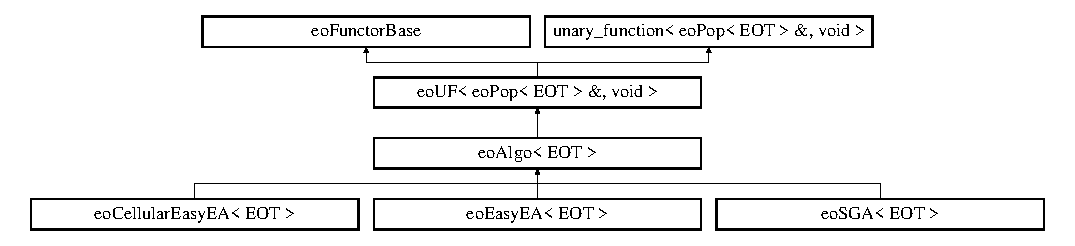
\includegraphics[height=2.86079cm]{classeo_algo}
\end{center}
\end{figure}


\subsection{Detailed Description}
\subsubsection*{template$<$class EOT$>$ class eo\-Algo$<$ EOT $>$}

This is a generic class for population-transforming algorithms. 

There is only one operator defined, which takes a population and does stuff to it. It needn't be a complete algorithm, can be also a step of an algorithm. This class just gives a common interface to linear population-transforming algorithms. 



Definition at line 39 of file eo\-Algo.h.

The documentation for this class was generated from the following file:\begin{CompactItemize}
\item 
eo\-Algo.h\end{CompactItemize}

\section{eo\-Arithmetic\-Crossover Class Reference}
\label{classeo_arithmetic_crossover}\index{eoArithmeticCrossover@{eoArithmeticCrossover}}
eo\-Hypercube\-Crossover --$>$ uniform choice in hypercube == arithmetical with different values for each coordinate  


{\tt \#include $<$Tutorial/eo\-Real\-Op.h$>$}



\subsection{Detailed Description}
eo\-Hypercube\-Crossover --$>$ uniform choice in hypercube == arithmetical with different values for each coordinate 



The documentation for this class was generated from the following file:\begin{CompactItemize}
\item 
eo\-Real\-Op.h\end{CompactItemize}

\section{eo\-Assembled\-Fitness\-Average\-Stat$<$ EOT $>$ Class Template Reference}
\label{classeo_assembled_fitness_average_stat}\index{eoAssembledFitnessAverageStat@{eoAssembledFitnessAverageStat}}
Average fitness values of a population, where the fitness is of type eo\-Scalar\-Assembled\-Fitness.  


{\tt \#include $<$eo\-Assembled\-Fitness\-Stat.h$>$}

Inheritance diagram for eo\-Assembled\-Fitness\-Average\-Stat$<$ EOT $>$::\begin{figure}[H]
\begin{center}
\leavevmode
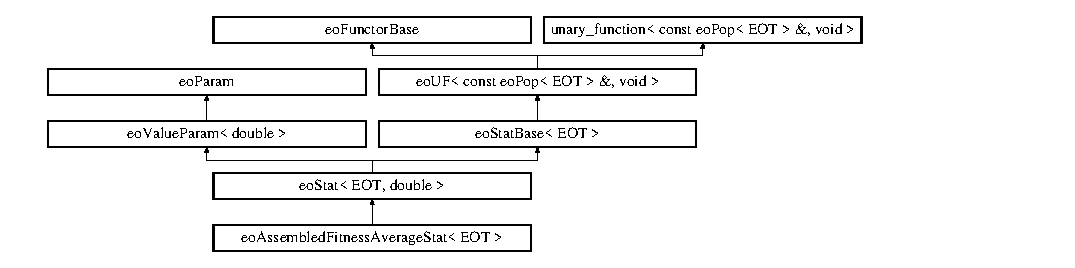
\includegraphics[height=3.15315cm]{classeo_assembled_fitness_average_stat}
\end{center}
\end{figure}
\subsection*{Public Types}
\begin{CompactItemize}
\item 
typedef EOT::Fitness {\bf Fitness}\label{classeo_assembled_fitness_average_stat_w0}

\end{CompactItemize}
\subsection*{Public Member Functions}
\begin{CompactItemize}
\item 
{\bf eo\-Assembled\-Fitness\-Average\-Stat} (unsigned \_\-which\-Term=0, std::string \_\-description=\char`\"{}Average Fitness\char`\"{})\label{classeo_assembled_fitness_average_stat_a0}

\item 
virtual void {\bf operator()} (const {\bf eo\-Pop}$<$ {\bf EOT} $>$ \&\_\-pop)\label{classeo_assembled_fitness_average_stat_a1}

\begin{CompactList}\small\item\em The pure virtual function that needs to be implemented by the subclass. \item\end{CompactList}\end{CompactItemize}
\subsection*{Private Attributes}
\begin{CompactItemize}
\item 
unsigned {\bf which\-Fitness\-Term}\label{classeo_assembled_fitness_average_stat_r0}

\end{CompactItemize}


\subsection{Detailed Description}
\subsubsection*{template$<$class EOT$>$ class eo\-Assembled\-Fitness\-Average\-Stat$<$ EOT $>$}

Average fitness values of a population, where the fitness is of type eo\-Scalar\-Assembled\-Fitness. 

Specify in the constructor, for which fitness term (index) the average should be evaluated. Only values of object where the failed boolean = false is set are counted. 



Definition at line 46 of file eo\-Assembled\-Fitness\-Stat.h.

The documentation for this class was generated from the following file:\begin{CompactItemize}
\item 
eo\-Assembled\-Fitness\-Stat.h\end{CompactItemize}

\section{eo\-Assembled\-Fitness\-Best\-Stat$<$ EOT $>$ Class Template Reference}
\label{classeo_assembled_fitness_best_stat}\index{eoAssembledFitnessBestStat@{eoAssembledFitnessBestStat}}
Fitness values of best individuum in a population, where the fitness is of type eo\-Scalar\-Assembled\-Fitness.  


{\tt \#include $<$eo\-Assembled\-Fitness\-Stat.h$>$}

Inheritance diagram for eo\-Assembled\-Fitness\-Best\-Stat$<$ EOT $>$::\begin{figure}[H]
\begin{center}
\leavevmode
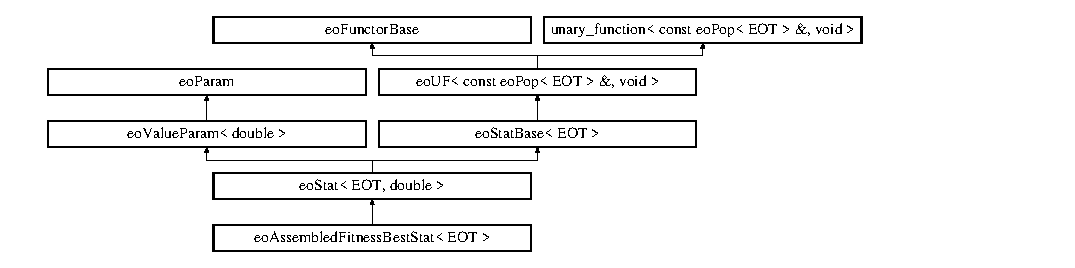
\includegraphics[height=3.15315cm]{classeo_assembled_fitness_best_stat}
\end{center}
\end{figure}
\subsection*{Public Types}
\begin{CompactItemize}
\item 
typedef EOT::Fitness {\bf Fitness}\label{classeo_assembled_fitness_best_stat_w0}

\end{CompactItemize}
\subsection*{Public Member Functions}
\begin{CompactItemize}
\item 
{\bf eo\-Assembled\-Fitness\-Best\-Stat} (unsigned \_\-which\-Term=0, std::string \_\-description=\char`\"{}Best Fitness\char`\"{})\label{classeo_assembled_fitness_best_stat_a0}

\item 
virtual void {\bf operator()} (const {\bf eo\-Pop}$<$ {\bf EOT} $>$ \&\_\-pop)\label{classeo_assembled_fitness_best_stat_a1}

\begin{CompactList}\small\item\em The pure virtual function that needs to be implemented by the subclass. \item\end{CompactList}\end{CompactItemize}
\subsection*{Private Attributes}
\begin{CompactItemize}
\item 
unsigned {\bf which\-Fitness\-Term}\label{classeo_assembled_fitness_best_stat_r0}

\end{CompactItemize}


\subsection{Detailed Description}
\subsubsection*{template$<$class EOT$>$ class eo\-Assembled\-Fitness\-Best\-Stat$<$ EOT $>$}

Fitness values of best individuum in a population, where the fitness is of type eo\-Scalar\-Assembled\-Fitness. 

Specify in the constructor, for which fitness term (index) the value should be evaluated. 



Definition at line 87 of file eo\-Assembled\-Fitness\-Stat.h.

The documentation for this class was generated from the following file:\begin{CompactItemize}
\item 
eo\-Assembled\-Fitness\-Stat.h\end{CompactItemize}

\section{eo\-Atom\-Exchange$<$ Atom $>$ Class Template Reference}
\label{classeo_atom_exchange}\index{eoAtomExchange@{eoAtomExchange}}
A helper class for choosing which genes to exchange.  


{\tt \#include $<$eo\-Variable\-Length\-Crossover.h$>$}

Inheritance diagram for eo\-Atom\-Exchange$<$ Atom $>$::\begin{figure}[H]
\begin{center}
\leavevmode
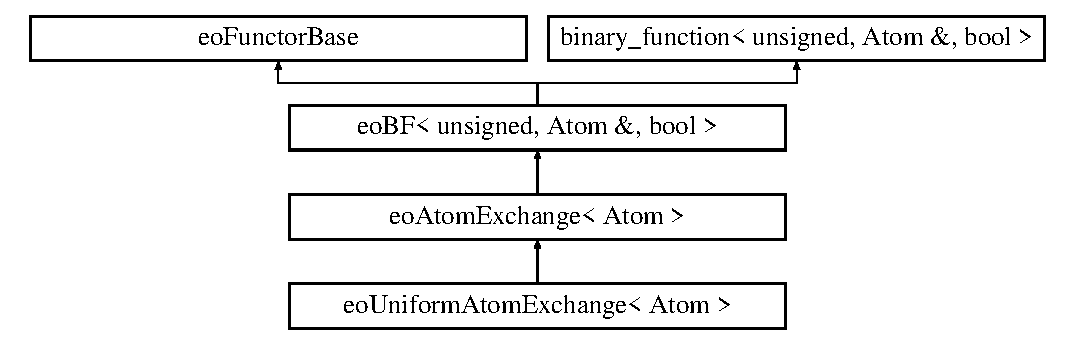
\includegraphics[height=4cm]{classeo_atom_exchange}
\end{center}
\end{figure}
\subsection*{Public Member Functions}
\begin{CompactItemize}
\item 
virtual void {\bf randomize} (unsigned int, unsigned int)\label{classeo_atom_exchange_a0}

\begin{CompactList}\small\item\em a function to initlialize - to be called before every crossover \item\end{CompactList}\item 
virtual std::string {\bf class\-Name} () const =0\label{classeo_atom_exchange_a1}

\begin{CompactList}\small\item\em the inherited {\bf class\-Name()}{\rm (p.\,\pageref{classeo_atom_exchange_a1})} \item\end{CompactList}\end{CompactItemize}


\subsection{Detailed Description}
\subsubsection*{template$<$class Atom$>$ class eo\-Atom\-Exchange$<$ Atom $>$}

A helper class for choosing which genes to exchange. 



Definition at line 41 of file eo\-Variable\-Length\-Crossover.h.

The documentation for this class was generated from the following file:\begin{CompactItemize}
\item 
eo\-Variable\-Length\-Crossover.h\end{CompactItemize}

\section{eo\-Average\-Stat$<$ EOT $>$ Class Template Reference}
\label{classeo_average_stat}\index{eoAverageStat@{eoAverageStat}}
Average fitness of a population.  


{\tt \#include $<$eo\-Stat.h$>$}

Inheritance diagram for eo\-Average\-Stat$<$ EOT $>$::\begin{figure}[H]
\begin{center}
\leavevmode
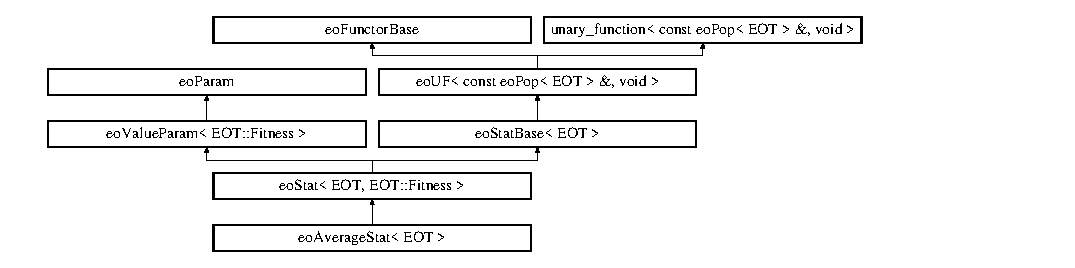
\includegraphics[height=3.15315cm]{classeo_average_stat}
\end{center}
\end{figure}
\subsection*{Public Types}
\begin{CompactItemize}
\item 
typedef EOT::Fitness {\bf Fitness}\label{classeo_average_stat_w0}

\end{CompactItemize}
\subsection*{Public Member Functions}
\begin{CompactItemize}
\item 
{\bf eo\-Average\-Stat} (std::string \_\-description=\char`\"{}Average Fitness\char`\"{})\label{classeo_average_stat_a0}

\item 
{\bf eo\-Average\-Stat} (double \_\-value, std::string \_\-desc)\label{classeo_average_stat_a1}

\item 
virtual void {\bf operator()} (const {\bf eo\-Pop}$<$ {\bf EOT} $>$ \&\_\-pop)\label{classeo_average_stat_a2}

\begin{CompactList}\small\item\em The pure virtual function that needs to be implemented by the subclass. \item\end{CompactList}\item 
virtual std::string {\bf class\-Name} (void) const \label{classeo_average_stat_a3}

\end{CompactItemize}
\subsection*{Static Public Member Functions}
\begin{CompactItemize}
\item 
Fitness {\bf sum\-Fitness} (double \_\-sum, const {\bf EOT} \&\_\-eot)\label{classeo_average_stat_e0}

\end{CompactItemize}
\subsection*{Private Member Functions}
\begin{CompactItemize}
\item 
template$<$class T$>$ void {\bf doit} (const {\bf eo\-Pop}$<$ {\bf EOT} $>$ \&\_\-pop, {\bf eo\-Pareto\-Fitness}$<$ T $>$)\label{classeo_average_stat_d0}

\item 
template$<$class T$>$ void {\bf doit} (const {\bf eo\-Pop}$<$ {\bf EOT} $>$ \&\_\-pop, T)\label{classeo_average_stat_d1}

\end{CompactItemize}


\subsection{Detailed Description}
\subsubsection*{template$<$class EOT$>$ class eo\-Average\-Stat$<$ EOT $>$}

Average fitness of a population. 

Fitness can be:\begin{itemize}
\item double\item eo\-Minimizing\-Fitness or eo\-Maximizing\-Fitness\item {\bf eo\-Pareto\-Fitness}{\rm (p.\,\pageref{classeo_pareto_fitness})}: The average of each objective is evaluated.\end{itemize}


( For {\bf eo\-Scalar\-Fitness\-Assembled}{\rm (p.\,\pageref{classeo_scalar_fitness_assembled})} user eo\-Assembled\-Fitness\-Stat classes.) 



Definition at line 108 of file eo\-Stat.h.

The documentation for this class was generated from the following file:\begin{CompactItemize}
\item 
eo\-Stat.h\end{CompactItemize}

\section{eo\-Best\-Fitness\-Stat$<$ EOT $>$ Class Template Reference}
\label{classeo_best_fitness_stat}\index{eoBestFitnessStat@{eoBestFitnessStat}}
Best fitness of a population.  


{\tt \#include $<$eo\-Stat.h$>$}

Inheritance diagram for eo\-Best\-Fitness\-Stat$<$ EOT $>$::\begin{figure}[H]
\begin{center}
\leavevmode
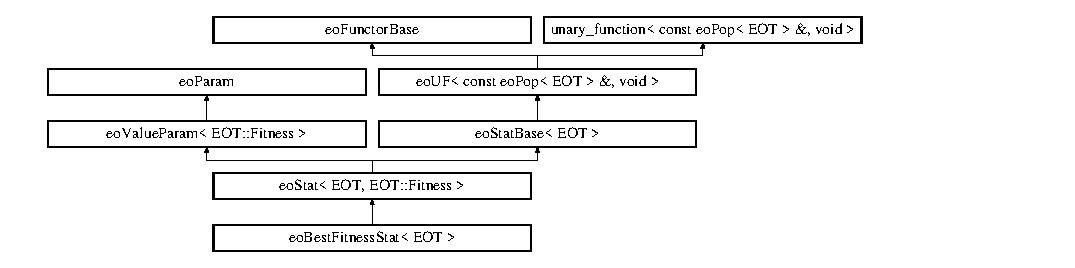
\includegraphics[height=3.15315cm]{classeo_best_fitness_stat}
\end{center}
\end{figure}
\subsection*{Public Types}
\begin{CompactItemize}
\item 
typedef EOT::Fitness {\bf Fitness}\label{classeo_best_fitness_stat_w0}

\end{CompactItemize}
\subsection*{Public Member Functions}
\begin{CompactItemize}
\item 
{\bf eo\-Best\-Fitness\-Stat} (std::string \_\-description=\char`\"{}Best \char`\"{})\label{classeo_best_fitness_stat_a0}

\item 
void {\bf operator()} (const {\bf eo\-Pop}$<$ {\bf EOT} $>$ \&\_\-pop)\label{classeo_best_fitness_stat_a1}

\begin{CompactList}\small\item\em The pure virtual function that needs to be implemented by the subclass. \item\end{CompactList}\item 
virtual std::string {\bf class\-Name} (void) const \label{classeo_best_fitness_stat_a2}

\end{CompactItemize}
\subsection*{Private Member Functions}
\begin{CompactItemize}
\item 
template$<$class T$>$ void {\bf doit} (const {\bf eo\-Pop}$<$ {\bf EOT} $>$ \&\_\-pop, {\bf eo\-Pareto\-Fitness}$<$ T $>$)\label{classeo_best_fitness_stat_d0}

\item 
template$<$class T$>$ void {\bf doit} (const {\bf eo\-Pop}$<$ {\bf EOT} $>$ \&\_\-pop, T)\label{classeo_best_fitness_stat_d1}

\end{CompactItemize}


\subsection{Detailed Description}
\subsubsection*{template$<$class EOT$>$ class eo\-Best\-Fitness\-Stat$<$ EOT $>$}

Best fitness of a population. 

Fitness can be:\begin{itemize}
\item double\item eo\-Minimizing\-Fitness or eo\-Maximizing\-Fitness\item {\bf eo\-Pareto\-Fitness}{\rm (p.\,\pageref{classeo_pareto_fitness})}:\end{itemize}


( For {\bf eo\-Scalar\-Fitness\-Assembled}{\rm (p.\,\pageref{classeo_scalar_fitness_assembled})} look at eo\-Assembled\-Fitness\-Stat ) 



Definition at line 316 of file eo\-Stat.h.

The documentation for this class was generated from the following file:\begin{CompactItemize}
\item 
eo\-Stat.h\end{CompactItemize}

\section{eo\-Best\-Select$<$ EOT $>$ Class Template Reference}
\label{classeo_best_select}\index{eoBestSelect@{eoBestSelect}}
eo\-Best\-Select: a selection method that always return the best (mainly for testing purposes)  


{\tt \#include $<$eo\-Random\-Select.h$>$}

Inheritance diagram for eo\-Best\-Select$<$ EOT $>$::\begin{figure}[H]
\begin{center}
\leavevmode
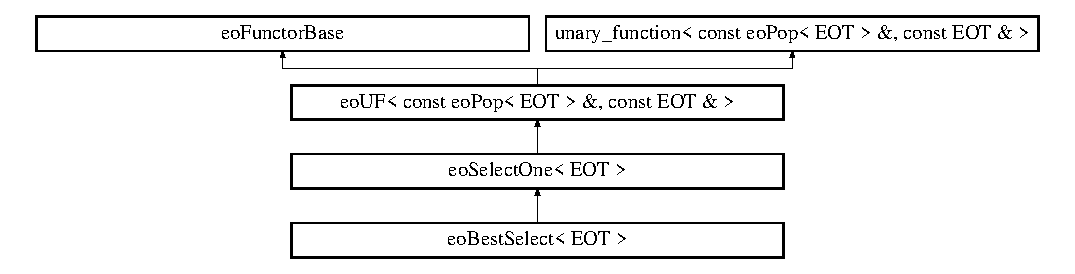
\includegraphics[height=3.23699cm]{classeo_best_select}
\end{center}
\end{figure}
\subsection*{Public Member Functions}
\begin{CompactItemize}
\item 
virtual const {\bf EOT} \& {\bf operator()} (const {\bf eo\-Pop}$<$ {\bf EOT} $>$ \&\_\-pop)\label{classeo_best_select_a0}

\begin{CompactList}\small\item\em not a big deal!!! \item\end{CompactList}\end{CompactItemize}


\subsection{Detailed Description}
\subsubsection*{template$<$class EOT$>$ class eo\-Best\-Select$<$ EOT $>$}

eo\-Best\-Select: a selection method that always return the best (mainly for testing purposes) 



Definition at line 60 of file eo\-Random\-Select.h.

The documentation for this class was generated from the following file:\begin{CompactItemize}
\item 
eo\-Random\-Select.h\end{CompactItemize}

\section{eo\-BF$<$ A1, A2, R $>$ Class Template Reference}
\label{classeo_b_f}\index{eoBF@{eoBF}}
Basic Binary Functor.  


{\tt \#include $<$eo\-Functor.h$>$}

Inheritance diagram for eo\-BF$<$ A1, A2, R $>$::\begin{figure}[H]
\begin{center}
\leavevmode
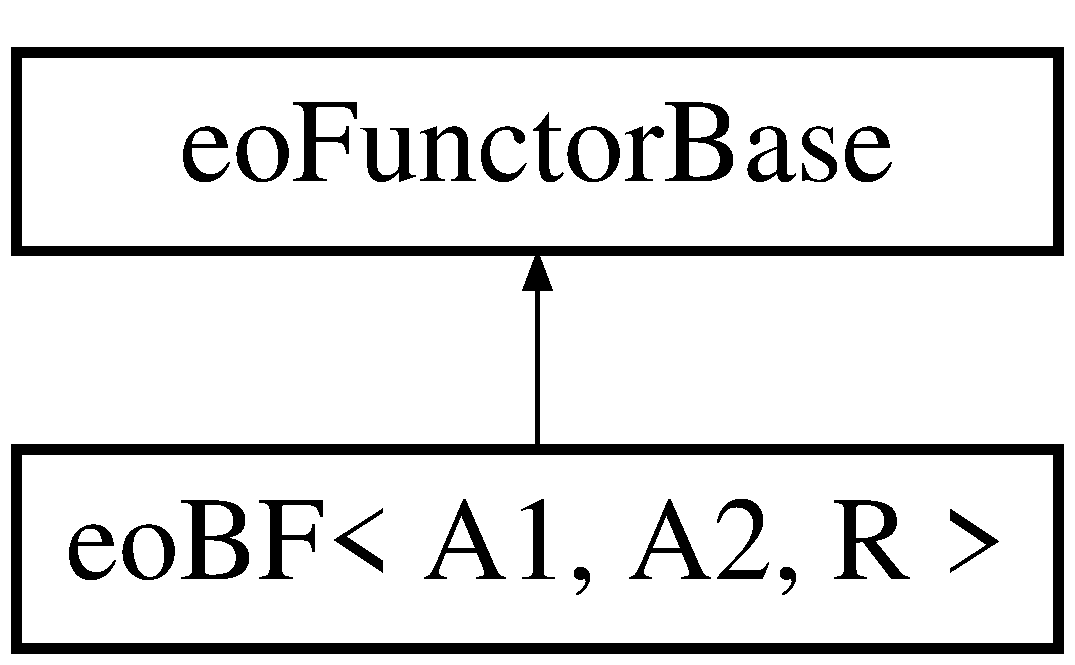
\includegraphics[height=2cm]{classeo_b_f}
\end{center}
\end{figure}
\subsection*{Public Member Functions}
\begin{CompactItemize}
\item 
virtual {\bf $\sim$eo\-BF} ()\label{classeo_b_f_a0}

\begin{CompactList}\small\item\em virtual dtor here so there is no need to define it in derived classes \item\end{CompactList}\item 
virtual R {\bf operator()} (A1, A2)=0\label{classeo_b_f_a1}

\begin{CompactList}\small\item\em The pure virtual function that needs to be implemented by the subclass. \item\end{CompactList}\end{CompactItemize}
\subsection*{Static Public Member Functions}
\begin{CompactItemize}
\item 
{\bf eo\-Functor\-Base::binary\_\-function\_\-tag} {\bf functor\_\-category} ()\label{classeo_b_f_e0}

\begin{CompactList}\small\item\em tag to identify a procedure in compile time function selection functor\_\-category \item\end{CompactList}\end{CompactItemize}


\subsection{Detailed Description}
\subsubsection*{template$<$class A1, class A2, class R$>$ class eo\-BF$<$ A1, A2, R $>$}

Basic Binary Functor. 

Derive from this class when defining any binary function. First template argument is result\_\-type, second is first\_\-argument\_\-type, third is second\_\-argument\_\-type. Argument and result types can be any type including void for result\_\-type 



Definition at line 145 of file eo\-Functor.h.

The documentation for this class was generated from the following file:\begin{CompactItemize}
\item 
eo\-Functor.h\end{CompactItemize}

\section{Biased\-Node\-Selector Class Reference}
\label{class_biased_node_selector}\index{BiasedNodeSelector@{BiasedNodeSelector}}
A node selector that does a specified number of rounds ignoring terminals.  


{\tt \#include $<$Node\-Selector.h$>$}

Inheritance diagram for Biased\-Node\-Selector::\begin{figure}[H]
\begin{center}
\leavevmode
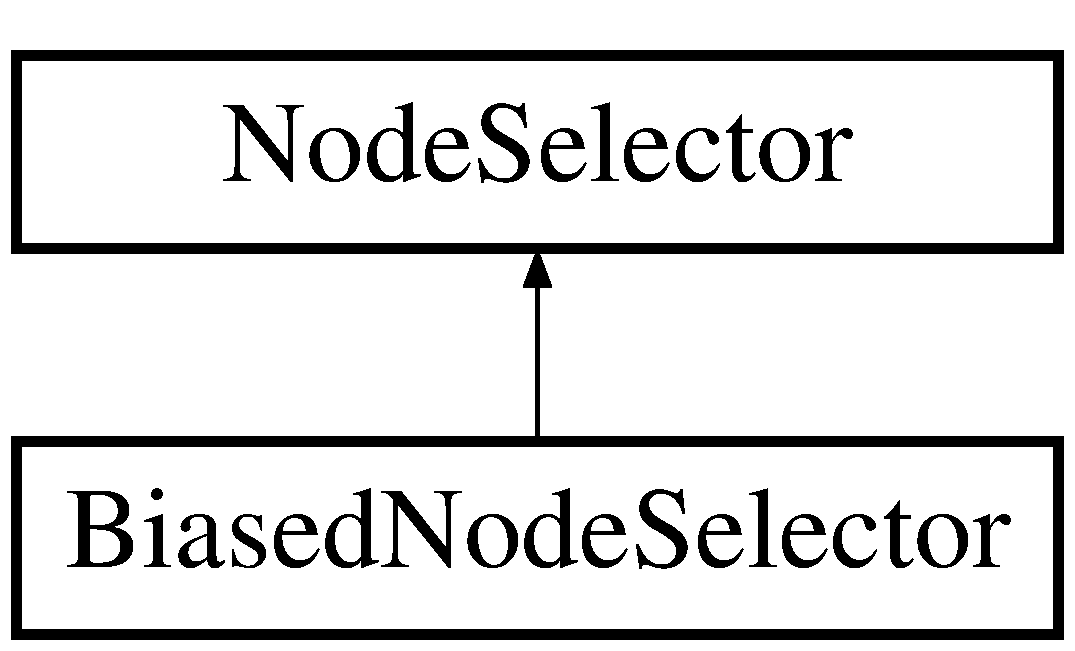
\includegraphics[height=2cm]{class_biased_node_selector}
\end{center}
\end{figure}
\subsection*{Public Member Functions}
\begin{CompactItemize}
\item 
{\bf Biased\-Node\-Selector} (unsigned n)\label{class_biased_node_selector_a1}

\item 
Node\-Selection {\bf select\_\-node} (Sym sym) const \label{class_biased_node_selector_a2}

\end{CompactItemize}
\subsection*{Public Attributes}
\begin{CompactItemize}
\item 
unsigned {\bf n\-Rounds}\label{class_biased_node_selector_o0}

\end{CompactItemize}


\subsection{Detailed Description}
A node selector that does a specified number of rounds ignoring terminals. 



Definition at line 55 of file Node\-Selector.h.

The documentation for this class was generated from the following files:\begin{CompactItemize}
\item 
Node\-Selector.h\item 
Node\-Selector.cpp\end{CompactItemize}

\section{eo\-Binary\-Functor\-Counter$<$ Binary\-Functor $>$ Class Template Reference}
\label{classeo_binary_functor_counter}\index{eoBinaryFunctorCounter@{eoBinaryFunctorCounter}}
Generic counter class that counts the number of times a binary function is used.  


{\tt \#include $<$eo\-Counter.h$>$}

Inheritance diagram for eo\-Binary\-Functor\-Counter$<$ Binary\-Functor $>$::\begin{figure}[H]
\begin{center}
\leavevmode
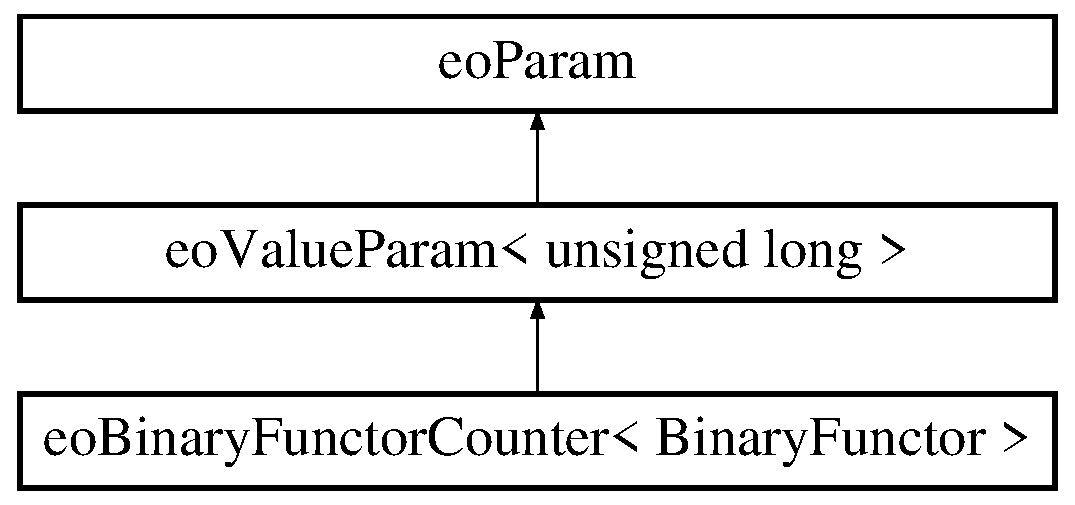
\includegraphics[height=3cm]{classeo_binary_functor_counter}
\end{center}
\end{figure}
\subsection*{Public Member Functions}
\begin{CompactItemize}
\item 
{\bf eo\-Binary\-Functor\-Counter} (Binary\-Functor \&\_\-func, std::string \_\-name=\char`\"{}proc\_\-counter\char`\"{})\label{classeo_binary_functor_counter_a0}

\item 
Binary\-Functor::result\_\-type {\bf operator()} (typename Binary\-Functor::first\_\-argument\_\-type \_\-arg1, typename Binary\-Functor::second\_\-argument\_\-type \_\-arg2)
\begin{CompactList}\small\item\em Calls the embedded function and increments the counter. \item\end{CompactList}\end{CompactItemize}
\subsection*{Private Attributes}
\begin{CompactItemize}
\item 
Binary\-Functor \& {\bf func}\label{classeo_binary_functor_counter_r0}

\end{CompactItemize}


\subsection{Detailed Description}
\subsubsection*{template$<$class Binary\-Functor$>$ class eo\-Binary\-Functor\-Counter$<$ Binary\-Functor $>$}

Generic counter class that counts the number of times a binary function is used. 

Add a binary function through its ctor and use this class instead of it.

It is derived from {\bf eo\-Value\-Param}{\rm (p.\,\pageref{classeo_value_param})} so you can add it to a monitor. 



Definition at line 142 of file eo\-Counter.h.

\subsection{Member Function Documentation}
\index{eoBinaryFunctorCounter@{eo\-Binary\-Functor\-Counter}!operator()@{operator()}}
\index{operator()@{operator()}!eoBinaryFunctorCounter@{eo\-Binary\-Functor\-Counter}}
\subsubsection{\setlength{\rightskip}{0pt plus 5cm}template$<$class Binary\-Functor$>$ Binary\-Functor::result\_\-type {\bf eo\-Binary\-Functor\-Counter}$<$ Binary\-Functor $>$::operator() (typename Binary\-Functor::first\_\-argument\_\-type {\em \_\-arg1}, typename Binary\-Functor::second\_\-argument\_\-type {\em \_\-arg2})\hspace{0.3cm}{\tt  [inline]}}\label{classeo_binary_functor_counter_a1}


Calls the embedded function and increments the counter. 

Note for MSVC users, if this code does not compile, you are quite likely trying to count a function that has a non-void return type. Don't look at us, look at the MSVC builders. Code like \char`\"{}return void;\char`\"{} is perfectly legal according to the ANSI standard, but the guys at Microsoft didn't get to implementing it yet.

We had two choices: assuming (and compiling ) code that returns void or code that returns non-void. Given that in {\bf EO}{\rm (p.\,\pageref{class_e_o})} most functors return void, it was chosen to support void.

But also please let me know if you have a compiler that defines \_\-MSC\_\-VER (lot's of windows compilers do), but is quite capable of compiling return void; type of code. We'll try to change the signature then.

You happy GNU (and other compiler) users will not have a problem with this. 

Definition at line 166 of file eo\-Counter.h.

References eo\-Value\-Param$<$ unsigned long $>$::value().

The documentation for this class was generated from the following file:\begin{CompactItemize}
\item 
eo\-Counter.h\end{CompactItemize}

\section{eo\-Bin\-Clone\-Op$<$ EOT $>$ Class Template Reference}
\label{classeo_bin_clone_op}\index{eoBinCloneOp@{eoBinCloneOp}}
Binary clone: two operands, only the first could be modified.  


{\tt \#include $<$eo\-Clone\-Ops.h$>$}

Inheritance diagram for eo\-Bin\-Clone\-Op$<$ EOT $>$::\begin{figure}[H]
\begin{center}
\leavevmode
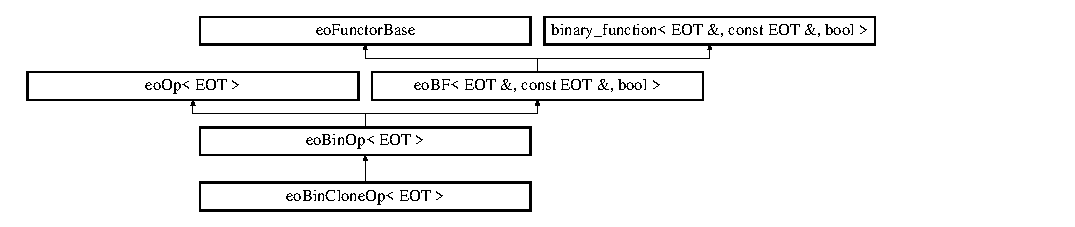
\includegraphics[height=2.60163cm]{classeo_bin_clone_op}
\end{center}
\end{figure}
\subsection*{Public Member Functions}
\begin{CompactItemize}
\item 
{\bf eo\-Bin\-Clone\-Op} ()\label{classeo_bin_clone_op_a0}

\begin{CompactList}\small\item\em Ctor. \item\end{CompactList}\item 
virtual std::string {\bf class\-Name} () const \label{classeo_bin_clone_op_a1}

\item 
virtual bool {\bf operator()} ({\bf EOT} \&, const {\bf EOT} \&)\label{classeo_bin_clone_op_a2}

\begin{CompactList}\small\item\em The pure virtual function that needs to be implemented by the subclass. \item\end{CompactList}\end{CompactItemize}


\subsection{Detailed Description}
\subsubsection*{template$<$class EOT$>$ class eo\-Bin\-Clone\-Op$<$ EOT $>$}

Binary clone: two operands, only the first could be modified. 



Definition at line 57 of file eo\-Clone\-Ops.h.

The documentation for this class was generated from the following file:\begin{CompactItemize}
\item 
eo\-Clone\-Ops.h\end{CompactItemize}

\section{eo\-Bin\-Gen\-Op$<$ EOT $>$ Class Template Reference}
\label{classeo_bin_gen_op}\index{eoBinGenOp@{eoBinGenOp}}
Wrapper for binop: here we use select method of {\bf eo\-Populator}{\rm (p.\,\pageref{classeo_populator})} but we could also have an embedded selector to select the second parent.  


{\tt \#include $<$eo\-Gen\-Op.h$>$}

Inheritance diagram for eo\-Bin\-Gen\-Op$<$ EOT $>$::\begin{figure}[H]
\begin{center}
\leavevmode
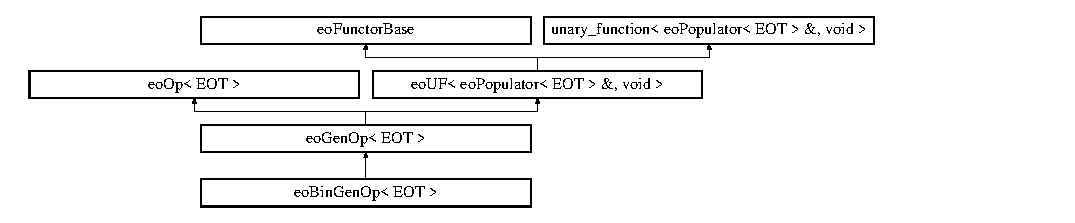
\includegraphics[height=2.54835cm]{classeo_bin_gen_op}
\end{center}
\end{figure}
\subsection*{Public Member Functions}
\begin{CompactItemize}
\item 
{\bf eo\-Bin\-Gen\-Op} ({\bf eo\-Bin\-Op}$<$ {\bf EOT} $>$ \&\_\-op)\label{classeo_bin_gen_op_a0}

\item 
unsigned {\bf max\_\-production} (void)\label{classeo_bin_gen_op_a1}

\begin{CompactList}\small\item\em Max production is used to reserve space for all elements that are used by the operator, not setting it properly can result in a crash. \item\end{CompactList}\item 
void {\bf apply} ({\bf eo\-Populator}$<$ {\bf EOT} $>$ \&\_\-pop)\label{classeo_bin_gen_op_a2}

\begin{CompactList}\small\item\em do the work: get 2 individuals from the population, modifies only one (it's a {\bf eo\-Bin\-Op}{\rm (p.\,\pageref{classeo_bin_op})}) \item\end{CompactList}\item 
virtual std::string {\bf class\-Name} () const \label{classeo_bin_gen_op_a3}

\end{CompactItemize}
\subsection*{Private Attributes}
\begin{CompactItemize}
\item 
{\bf eo\-Bin\-Op}$<$ {\bf EOT} $>$ \& {\bf op}\label{classeo_bin_gen_op_r0}

\end{CompactItemize}


\subsection{Detailed Description}
\subsubsection*{template$<$class EOT$>$ class eo\-Bin\-Gen\-Op$<$ EOT $>$}

Wrapper for binop: here we use select method of {\bf eo\-Populator}{\rm (p.\,\pageref{classeo_populator})} but we could also have an embedded selector to select the second parent. 



Definition at line 107 of file eo\-Gen\-Op.h.

The documentation for this class was generated from the following file:\begin{CompactItemize}
\item 
eo\-Gen\-Op.h\end{CompactItemize}

\section{eo\-Bin\-Op$<$ EOType $>$ Class Template Reference}
\label{classeo_bin_op}\index{eoBinOp@{eoBinOp}}
Binary genetic operator: subclasses {\bf eo\-Op}{\rm (p.\,\pageref{classeo_op})}, and defines basically the operator() with two operands, only the first one can be modified When defining your own, make sure that you return a boolean value indicating that you have changed the content.  


{\tt \#include $<$eo\-Op.h$>$}

Inheritance diagram for eo\-Bin\-Op$<$ EOType $>$::\begin{figure}[H]
\begin{center}
\leavevmode
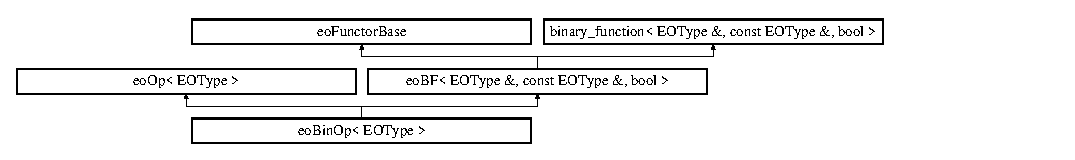
\includegraphics[height=1.70213cm]{classeo_bin_op}
\end{center}
\end{figure}
\subsection*{Public Member Functions}
\begin{CompactItemize}
\item 
{\bf eo\-Bin\-Op} ()\label{classeo_bin_op_a0}

\begin{CompactList}\small\item\em Ctor. \item\end{CompactList}\item 
virtual std::string {\bf class\-Name} () const \label{classeo_bin_op_a1}

\end{CompactItemize}


\subsection{Detailed Description}
\subsubsection*{template$<$class EOType$>$ class eo\-Bin\-Op$<$ EOType $>$}

Binary genetic operator: subclasses {\bf eo\-Op}{\rm (p.\,\pageref{classeo_op})}, and defines basically the operator() with two operands, only the first one can be modified When defining your own, make sure that you return a boolean value indicating that you have changed the content. 



Definition at line 117 of file eo\-Op.h.

The documentation for this class was generated from the following file:\begin{CompactItemize}
\item 
eo\-Op.h\end{CompactItemize}

\section{eo\-Bit$<$ Fit\-T $>$ Class Template Reference}
\label{classeo_bit}\index{eoBit@{eoBit}}
Implementation of bitstring chromosome.  


{\tt \#include $<$ga/eo\-Bit.h$>$}

Inheritance diagram for eo\-Bit$<$ Fit\-T $>$::\begin{figure}[H]
\begin{center}
\leavevmode
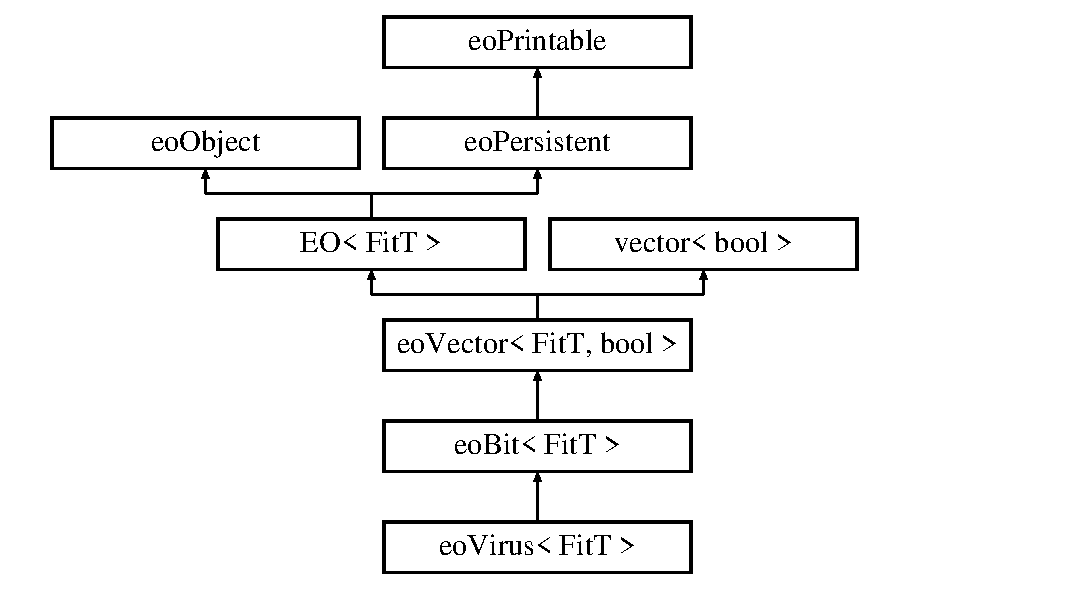
\includegraphics[height=6cm]{classeo_bit}
\end{center}
\end{figure}
\subsection*{Public Member Functions}
\begin{CompactItemize}
\item 
{\bf eo\-Bit} (unsigned size=0, bool value=false)
\begin{CompactList}\small\item\em (Default) Constructor. \item\end{CompactList}\item 
virtual std::string {\bf class\-Name} () const \label{classeo_bit_a1}

\begin{CompactList}\small\item\em My class name. \item\end{CompactList}\item 
virtual void {\bf print\-On} (std::ostream \&os) const 
\begin{CompactList}\small\item\em To print me on a stream. \item\end{CompactList}\item 
virtual void {\bf read\-From} (std::istream \&is)
\begin{CompactList}\small\item\em To read me from a stream. \item\end{CompactList}\end{CompactItemize}


\subsection{Detailed Description}
\subsubsection*{template$<$class Fit\-T$>$ class eo\-Bit$<$ Fit\-T $>$}

Implementation of bitstring chromosome. 

Based on STL's vector$<$bool$>$ specialization. 



Definition at line 56 of file eo\-Bit.h.

\subsection{Constructor \& Destructor Documentation}
\index{eoBit@{eo\-Bit}!eoBit@{eoBit}}
\index{eoBit@{eoBit}!eoBit@{eo\-Bit}}
\subsubsection{\setlength{\rightskip}{0pt plus 5cm}template$<$class Fit\-T$>$ {\bf eo\-Bit}$<$ {\bf Fit\-T} $>$::{\bf eo\-Bit} (unsigned {\em size} = {\tt 0}, bool {\em value} = {\tt false})\hspace{0.3cm}{\tt  [inline]}}\label{classeo_bit_a0}


(Default) Constructor. 

\begin{Desc}
\item[Parameters:]
\begin{description}
\item[{\em size}]Size of the binary std::string. \end{description}
\end{Desc}


Definition at line 69 of file eo\-Bit.h.

\subsection{Member Function Documentation}
\index{eoBit@{eo\-Bit}!printOn@{printOn}}
\index{printOn@{printOn}!eoBit@{eo\-Bit}}
\subsubsection{\setlength{\rightskip}{0pt plus 5cm}template$<$class Fit\-T$>$ virtual void {\bf eo\-Bit}$<$ {\bf Fit\-T} $>$::print\-On (std::ostream \& {\em os}) const\hspace{0.3cm}{\tt  [inline, virtual]}}\label{classeo_bit_a2}


To print me on a stream. 

\begin{Desc}
\item[Parameters:]
\begin{description}
\item[{\em os}]The std::ostream. \end{description}
\end{Desc}


Reimplemented from {\bf eo\-Vector$<$ Fit\-T, bool $>$} {\rm (p.\,\pageref{classeo_vector_a4})}.

Definition at line 82 of file eo\-Bit.h.

References EO$<$ F $>$::print\-On().\index{eoBit@{eo\-Bit}!readFrom@{readFrom}}
\index{readFrom@{readFrom}!eoBit@{eo\-Bit}}
\subsubsection{\setlength{\rightskip}{0pt plus 5cm}template$<$class Fit\-T$>$ virtual void {\bf eo\-Bit}$<$ {\bf Fit\-T} $>$::read\-From (std::istream \& {\em is})\hspace{0.3cm}{\tt  [inline, virtual]}}\label{classeo_bit_a3}


To read me from a stream. 

\begin{Desc}
\item[Parameters:]
\begin{description}
\item[{\em is}]The std::istream. \end{description}
\end{Desc}


Reimplemented from {\bf eo\-Vector$<$ Fit\-T, bool $>$} {\rm (p.\,\pageref{classeo_vector_a5})}.

Definition at line 94 of file eo\-Bit.h.

References EO$<$ F $>$::read\-From().

The documentation for this class was generated from the following file:\begin{CompactItemize}
\item 
eo\-Bit.h\end{CompactItemize}

\section{eo\-Bit\-Bit\-Flip Class Reference}
\label{classeo_bit_bit_flip}\index{eoBitBitFlip@{eoBitBitFlip}}
eo\-Bit\-Flip --$>$ changes 1 bit  


{\tt \#include $<$ga/eo\-Bit\-Op.h$>$}



\subsection{Detailed Description}
eo\-Bit\-Flip --$>$ changes 1 bit 



The documentation for this class was generated from the following file:\begin{CompactItemize}
\item 
eo\-Bit\-Op.h\end{CompactItemize}

\section{eo\-Bit\-Gx\-Over$<$ Chrom $>$ Class Template Reference}
\label{classeo_bit_gx_over}\index{eoBitGxOver@{eoBitGxOver}}
eo\-Bit\-Gx\-Over --$>$ Npts crossover when bistd::string considered as a std::string of binary-encoded genes (exchanges genes) Is anybody still using it apart from historians ??? :-)  


{\tt \#include $<$ga/eo\-Bit\-Op.h$>$}

Inheritance diagram for eo\-Bit\-Gx\-Over$<$ Chrom $>$::\begin{figure}[H]
\begin{center}
\leavevmode
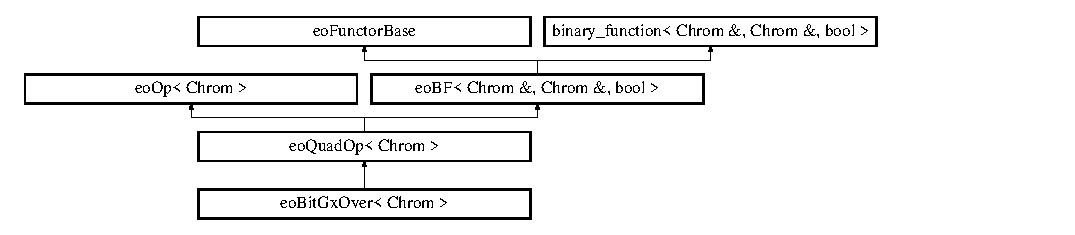
\includegraphics[height=2.70531cm]{classeo_bit_gx_over}
\end{center}
\end{figure}
\subsection*{Public Member Functions}
\begin{CompactItemize}
\item 
{\bf eo\-Bit\-Gx\-Over} (const unsigned \_\-gene\_\-size, const unsigned \_\-num\_\-points=2)\label{classeo_bit_gx_over_a0}

\begin{CompactList}\small\item\em Constructor. \item\end{CompactList}\item 
virtual std::string {\bf class\-Name} () const \label{classeo_bit_gx_over_a1}

\begin{CompactList}\small\item\em The class name. \item\end{CompactList}\item 
bool {\bf operator()} (Chrom \&chrom1, Chrom \&chrom2)
\begin{CompactList}\small\item\em Gene crossover for binary chromosomes. \item\end{CompactList}\end{CompactItemize}
\subsection*{Private Attributes}
\begin{CompactItemize}
\item 
unsigned {\bf gene\_\-size}\label{classeo_bit_gx_over_r0}

\item 
unsigned {\bf num\_\-points}\label{classeo_bit_gx_over_r1}

\end{CompactItemize}


\subsection{Detailed Description}
\subsubsection*{template$<$class Chrom$>$ class eo\-Bit\-Gx\-Over$<$ Chrom $>$}

eo\-Bit\-Gx\-Over --$>$ Npts crossover when bistd::string considered as a std::string of binary-encoded genes (exchanges genes) Is anybody still using it apart from historians ??? :-) 



Definition at line 388 of file eo\-Bit\-Op.h.

\subsection{Member Function Documentation}
\index{eoBitGxOver@{eo\-Bit\-Gx\-Over}!operator()@{operator()}}
\index{operator()@{operator()}!eoBitGxOver@{eo\-Bit\-Gx\-Over}}
\subsubsection{\setlength{\rightskip}{0pt plus 5cm}template$<$class Chrom$>$ bool {\bf eo\-Bit\-Gx\-Over}$<$ Chrom $>$::operator() (Chrom \& {\em chrom1}, Chrom \& {\em chrom2})\hspace{0.3cm}{\tt  [inline, virtual]}}\label{classeo_bit_gx_over_a2}


Gene crossover for binary chromosomes. 

\begin{Desc}
\item[Parameters:]
\begin{description}
\item[{\em chrom1}]The first chromosome. \item[{\em chrom2}]The first chromosome. \end{description}
\end{Desc}


Implements {\bf eo\-BF$<$ Chrom \&, Chrom \&, bool $>$} {\rm (p.\,\pageref{classeo_b_f_a1})}.

Definition at line 409 of file eo\-Bit\-Op.h.

The documentation for this class was generated from the following file:\begin{CompactItemize}
\item 
eo\-Bit\-Op.h\end{CompactItemize}

\section{eo\-Bit\-Inversion$<$ Chrom $>$ Class Template Reference}
\label{classeo_bit_inversion}\index{eoBitInversion@{eoBitInversion}}
eo\-Bit\-Inversion: inverts the bits of the chromosome between an interval  


{\tt \#include $<$ga/eo\-Bit\-Op.h$>$}

Inheritance diagram for eo\-Bit\-Inversion$<$ Chrom $>$::\begin{figure}[H]
\begin{center}
\leavevmode
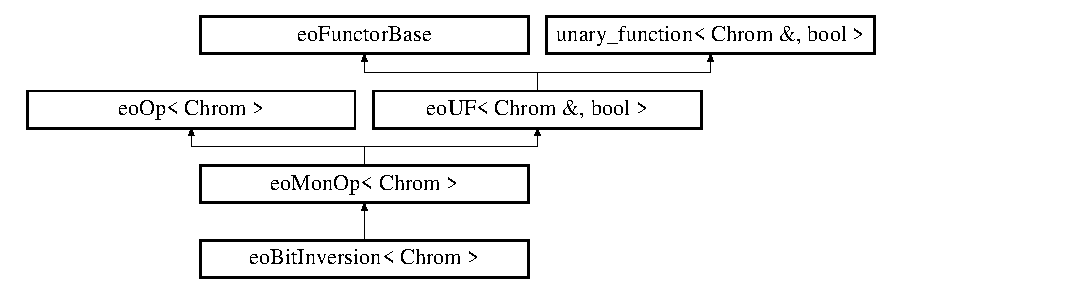
\includegraphics[height=3.50548cm]{classeo_bit_inversion}
\end{center}
\end{figure}
\subsection*{Public Member Functions}
\begin{CompactItemize}
\item 
virtual std::string {\bf class\-Name} () const \label{classeo_bit_inversion_a0}

\begin{CompactList}\small\item\em The class name. \item\end{CompactList}\item 
bool {\bf operator()} (Chrom \&chrom)
\begin{CompactList}\small\item\em Inverts a range of bits in a binary chromosome. \item\end{CompactList}\end{CompactItemize}


\subsection{Detailed Description}
\subsubsection*{template$<$class Chrom$>$ class eo\-Bit\-Inversion$<$ Chrom $>$}

eo\-Bit\-Inversion: inverts the bits of the chromosome between an interval 



Definition at line 146 of file eo\-Bit\-Op.h.

\subsection{Member Function Documentation}
\index{eoBitInversion@{eo\-Bit\-Inversion}!operator()@{operator()}}
\index{operator()@{operator()}!eoBitInversion@{eo\-Bit\-Inversion}}
\subsubsection{\setlength{\rightskip}{0pt plus 5cm}template$<$class Chrom$>$ bool {\bf eo\-Bit\-Inversion}$<$ Chrom $>$::operator() (Chrom \& {\em chrom})\hspace{0.3cm}{\tt  [inline, virtual]}}\label{classeo_bit_inversion_a1}


Inverts a range of bits in a binary chromosome. 

\begin{Desc}
\item[Parameters:]
\begin{description}
\item[{\em chrom}]The chromosome whos bits are going to be inverted (a range). \end{description}
\end{Desc}


Implements {\bf eo\-UF$<$ Chrom \&, bool $>$} {\rm (p.\,\pageref{classeo_u_f_a1})}.

Definition at line 156 of file eo\-Bit\-Op.h.

The documentation for this class was generated from the following file:\begin{CompactItemize}
\item 
eo\-Bit\-Op.h\end{CompactItemize}

\section{eo\-Bit\-Mutation$<$ Chrom $>$ Class Template Reference}
\label{classeo_bit_mutation}\index{eoBitMutation@{eoBitMutation}}
eo\-Bit\-Mutation --$>$ classical mutation  


{\tt \#include $<$ga/eo\-Bit\-Op.h$>$}

Inheritance diagram for eo\-Bit\-Mutation$<$ Chrom $>$::\begin{figure}[H]
\begin{center}
\leavevmode
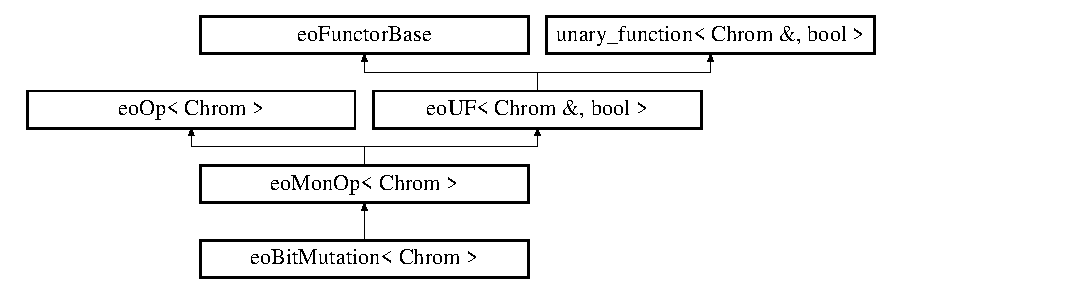
\includegraphics[height=3.50548cm]{classeo_bit_mutation}
\end{center}
\end{figure}
\subsection*{Public Member Functions}
\begin{CompactItemize}
\item 
{\bf eo\-Bit\-Mutation} (const double \&\_\-rate=0.01, bool \_\-normalize=false)
\begin{CompactList}\small\item\em (Default) Constructor. \item\end{CompactList}\item 
virtual std::string {\bf class\-Name} () const \label{classeo_bit_mutation_a1}

\begin{CompactList}\small\item\em The class name. \item\end{CompactList}\item 
bool {\bf operator()} (Chrom \&chrom)
\begin{CompactList}\small\item\em Mutate a chromosome. \item\end{CompactList}\end{CompactItemize}
\subsection*{Private Attributes}
\begin{CompactItemize}
\item 
double {\bf rate}\label{classeo_bit_mutation_r0}

\item 
bool {\bf normalize}\label{classeo_bit_mutation_r1}

\end{CompactItemize}


\subsection{Detailed Description}
\subsubsection*{template$<$class Chrom$>$ class eo\-Bit\-Mutation$<$ Chrom $>$}

eo\-Bit\-Mutation --$>$ classical mutation 



Definition at line 104 of file eo\-Bit\-Op.h.

\subsection{Constructor \& Destructor Documentation}
\index{eoBitMutation@{eo\-Bit\-Mutation}!eoBitMutation@{eoBitMutation}}
\index{eoBitMutation@{eoBitMutation}!eoBitMutation@{eo\-Bit\-Mutation}}
\subsubsection{\setlength{\rightskip}{0pt plus 5cm}template$<$class Chrom$>$ {\bf eo\-Bit\-Mutation}$<$ Chrom $>$::{\bf eo\-Bit\-Mutation} (const double \& {\em \_\-rate} = {\tt 0.01}, bool {\em \_\-normalize} = {\tt false})\hspace{0.3cm}{\tt  [inline]}}\label{classeo_bit_mutation_a0}


(Default) Constructor. 

\begin{Desc}
\item[Parameters:]
\begin{description}
\item[{\em \_\-rate}]Rate of mutation. \end{description}
\end{Desc}


Definition at line 111 of file eo\-Bit\-Op.h.

\subsection{Member Function Documentation}
\index{eoBitMutation@{eo\-Bit\-Mutation}!operator()@{operator()}}
\index{operator()@{operator()}!eoBitMutation@{eo\-Bit\-Mutation}}
\subsubsection{\setlength{\rightskip}{0pt plus 5cm}template$<$class Chrom$>$ bool {\bf eo\-Bit\-Mutation}$<$ Chrom $>$::operator() (Chrom \& {\em chrom})\hspace{0.3cm}{\tt  [inline, virtual]}}\label{classeo_bit_mutation_a2}


Mutate a chromosome. 

\begin{Desc}
\item[Parameters:]
\begin{description}
\item[{\em chrom}]The chromosome to be mutated. \end{description}
\end{Desc}


Implements {\bf eo\-UF$<$ Chrom \&, bool $>$} {\rm (p.\,\pageref{classeo_u_f_a1})}.

Definition at line 121 of file eo\-Bit\-Op.h.

The documentation for this class was generated from the following file:\begin{CompactItemize}
\item 
eo\-Bit\-Op.h\end{CompactItemize}

\section{eo\-Bit\-Next$<$ Chrom $>$ Class Template Reference}
\label{classeo_bit_next}\index{eoBitNext@{eoBitNext}}
eo\-Bit\-Next --$>$ next value when bitstring considered as binary value  


{\tt \#include $<$ga/eo\-Bit\-Op.h$>$}

Inheritance diagram for eo\-Bit\-Next$<$ Chrom $>$::\begin{figure}[H]
\begin{center}
\leavevmode
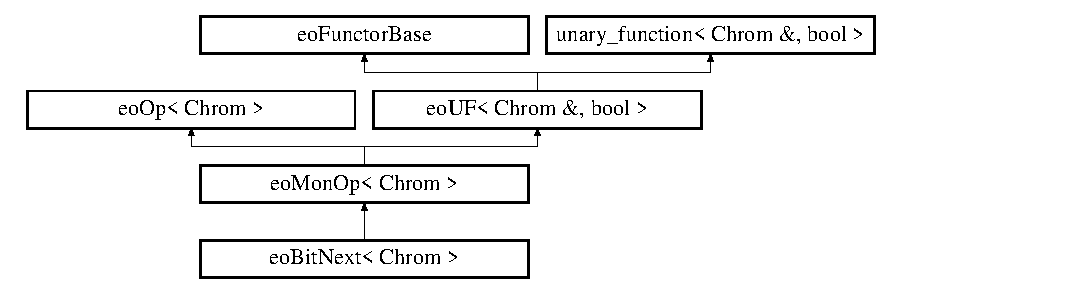
\includegraphics[height=3.50548cm]{classeo_bit_next}
\end{center}
\end{figure}
\subsection*{Public Member Functions}
\begin{CompactItemize}
\item 
virtual std::string {\bf class\-Name} () const \label{classeo_bit_next_a0}

\begin{CompactList}\small\item\em The class name. \item\end{CompactList}\item 
bool {\bf operator()} (Chrom \&chrom)
\begin{CompactList}\small\item\em Change the bit std::string x to be x+1. \item\end{CompactList}\end{CompactItemize}


\subsection{Detailed Description}
\subsubsection*{template$<$class Chrom$>$ class eo\-Bit\-Next$<$ Chrom $>$}

eo\-Bit\-Next --$>$ next value when bitstring considered as binary value 



Definition at line 174 of file eo\-Bit\-Op.h.

\subsection{Member Function Documentation}
\index{eoBitNext@{eo\-Bit\-Next}!operator()@{operator()}}
\index{operator()@{operator()}!eoBitNext@{eo\-Bit\-Next}}
\subsubsection{\setlength{\rightskip}{0pt plus 5cm}template$<$class Chrom$>$ bool {\bf eo\-Bit\-Next}$<$ Chrom $>$::operator() (Chrom \& {\em chrom})\hspace{0.3cm}{\tt  [inline, virtual]}}\label{classeo_bit_next_a1}


Change the bit std::string x to be x+1. 

\begin{Desc}
\item[Parameters:]
\begin{description}
\item[{\em chrom}]The chromosome to be added one. \end{description}
\end{Desc}


Implements {\bf eo\-UF$<$ Chrom \&, bool $>$} {\rm (p.\,\pageref{classeo_u_f_a1})}.

Definition at line 184 of file eo\-Bit\-Op.h.

The documentation for this class was generated from the following file:\begin{CompactItemize}
\item 
eo\-Bit\-Op.h\end{CompactItemize}

\section{eo\-Bit\-Op\-Factory$<$ EOT $>$ Class Template Reference}
\label{classeo_bit_op_factory}\index{eoBitOpFactory@{eoBitOpFactory}}
{\bf EO}{\rm (p.\,\pageref{class_e_o})} Factory.  


{\tt \#include $<$eo\-Bit\-Op\-Factory.h$>$}

Inheritance diagram for eo\-Bit\-Op\-Factory$<$ EOT $>$::\begin{figure}[H]
\begin{center}
\leavevmode
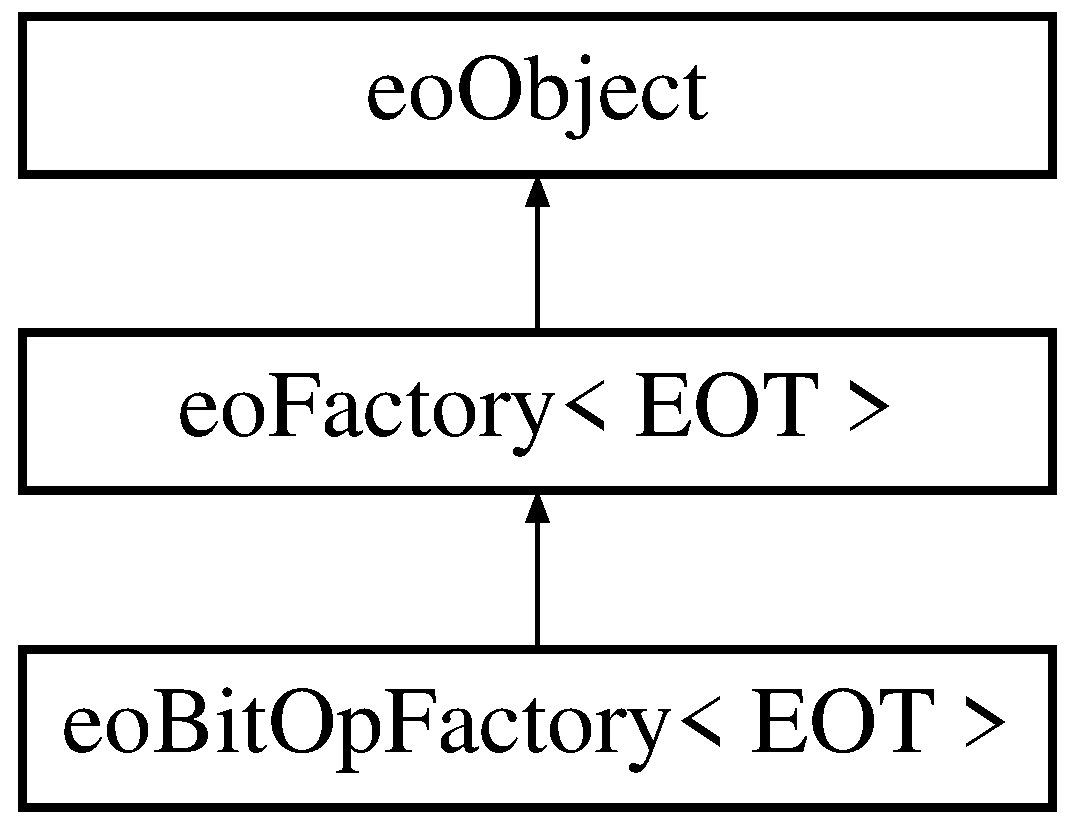
\includegraphics[height=3cm]{classeo_bit_op_factory}
\end{center}
\end{figure}
\subsection*{Public Member Functions}
\begin{CompactItemize}
\item 
virtual {\bf eo\-Op}$<$ {\bf EOT} $>$ $\ast$ {\bf make} (std::istream \&\_\-is)
\begin{CompactList}\small\item\em Another factory method: creates an object from an std::istream, reading from it whatever is needed to create the object. \item\end{CompactList}\end{CompactItemize}
\begin{Indent}{\bf ctors and dtors}\par
\begin{CompactItemize}
\item 
{\bf eo\-Bit\-Op\-Factory} ()\label{classeo_bit_op_factory_z23_0}

\begin{CompactList}\small\item\em constructor \item\end{CompactList}\item 
virtual {\bf $\sim$eo\-Bit\-Op\-Factory} ()\label{classeo_bit_op_factory_z23_1}

\begin{CompactList}\small\item\em destructor \item\end{CompactList}\end{CompactItemize}
\end{Indent}


\subsection{Detailed Description}
\subsubsection*{template$<$class EOT$>$ class eo\-Bit\-Op\-Factory$<$ EOT $>$}

{\bf EO}{\rm (p.\,\pageref{class_e_o})} Factory. 

An instance of the factory class to create operators that act on bitstring chromosomes. Only those chromosomes can instantiate the operators that are created here \begin{Desc}
\item[See also:]{\bf eo\-Select}{\rm (p.\,\pageref{classeo_select})} \end{Desc}




Definition at line 39 of file eo\-Bit\-Op\-Factory.h.

\subsection{Member Function Documentation}
\index{eoBitOpFactory@{eo\-Bit\-Op\-Factory}!make@{make}}
\index{make@{make}!eoBitOpFactory@{eo\-Bit\-Op\-Factory}}
\subsubsection{\setlength{\rightskip}{0pt plus 5cm}template$<$class EOT$>$ virtual {\bf eo\-Op}$<${\bf EOT}$>$$\ast$ {\bf eo\-Bit\-Op\-Factory}$<$ {\bf EOT} $>$::make (std::istream \& {\em \_\-is})\hspace{0.3cm}{\tt  [inline, virtual]}}\label{classeo_bit_op_factory_a0}


Another factory method: creates an object from an std::istream, reading from it whatever is needed to create the object. 

Usually, the format for the std::istream will be$\backslash$ object\-Type parameter1 parameter2 ... parametern$\backslash$ If there are problems, an std::exception is raised; it should be caught at the upper level, because it might be something for that level$\backslash$ At the same time, it catches std::exceptions thrown at a lower level, which will indicate that whatever is in the stream is for this method to process \begin{Desc}
\item[Parameters:]
\begin{description}
\item[{\em \_\-is}]an stream from where a single line will be read \end{description}
\end{Desc}
\begin{Desc}
\item[Exceptions:]
\begin{description}
\item[{\em runtime\_\-std::exception}]if the object type is not known\end{description}
\end{Desc}


Implements {\bf eo\-Factory$<$ EOT $>$} {\rm (p.\,\pageref{classeo_factory_a0})}.

Definition at line 63 of file eo\-Bit\-Op\-Factory.h.

References eo\-Factory$<$ EOClass $>$::make().

The documentation for this class was generated from the following file:\begin{CompactItemize}
\item 
eo\-Bit\-Op\-Factory.h\end{CompactItemize}

\section{eo\-Bit\-Prev$<$ Chrom $>$ Class Template Reference}
\label{classeo_bit_prev}\index{eoBitPrev@{eoBitPrev}}
eo\-Bit\-Prev --$>$ previous value when bitstring treated as binary value  


{\tt \#include $<$ga/eo\-Bit\-Op.h$>$}

Inheritance diagram for eo\-Bit\-Prev$<$ Chrom $>$::\begin{figure}[H]
\begin{center}
\leavevmode
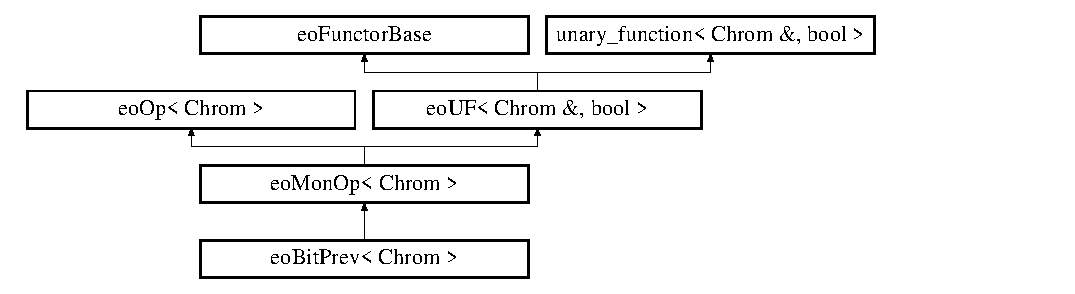
\includegraphics[height=3.50548cm]{classeo_bit_prev}
\end{center}
\end{figure}
\subsection*{Public Member Functions}
\begin{CompactItemize}
\item 
virtual std::string {\bf class\-Name} () const \label{classeo_bit_prev_a0}

\begin{CompactList}\small\item\em The class name. \item\end{CompactList}\item 
bool {\bf operator()} (Chrom \&chrom)
\begin{CompactList}\small\item\em Change the bit std::string x to be x-1. \item\end{CompactList}\end{CompactItemize}


\subsection{Detailed Description}
\subsubsection*{template$<$class Chrom$>$ class eo\-Bit\-Prev$<$ Chrom $>$}

eo\-Bit\-Prev --$>$ previous value when bitstring treated as binary value 



Definition at line 208 of file eo\-Bit\-Op.h.

\subsection{Member Function Documentation}
\index{eoBitPrev@{eo\-Bit\-Prev}!operator()@{operator()}}
\index{operator()@{operator()}!eoBitPrev@{eo\-Bit\-Prev}}
\subsubsection{\setlength{\rightskip}{0pt plus 5cm}template$<$class Chrom$>$ bool {\bf eo\-Bit\-Prev}$<$ Chrom $>$::operator() (Chrom \& {\em chrom})\hspace{0.3cm}{\tt  [inline, virtual]}}\label{classeo_bit_prev_a1}


Change the bit std::string x to be x-1. 

\begin{Desc}
\item[Parameters:]
\begin{description}
\item[{\em chrom}]The chromosome to be substracted one. \end{description}
\end{Desc}


Implements {\bf eo\-UF$<$ Chrom \&, bool $>$} {\rm (p.\,\pageref{classeo_u_f_a1})}.

Definition at line 218 of file eo\-Bit\-Op.h.

The documentation for this class was generated from the following file:\begin{CompactItemize}
\item 
eo\-Bit\-Op.h\end{CompactItemize}

\section{boolean\_\-generator Class Reference}
\label{classboolean__generator}\index{boolean_generator@{boolean\_\-generator}}
The class boolean\_\-generator can be used in the STL generate function to easily generate random booleans with a specified bias.  


{\tt \#include $<$rnd\_\-generators.h$>$}

\subsection*{Public Member Functions}
\begin{CompactItemize}
\item 
{\bf boolean\_\-generator} (float \_\-bias=0.5, {\bf eo\-Rng} \&\_\-rng=rng)\label{classboolean__generator_a0}

\item 
bool {\bf operator()} (void)\label{classboolean__generator_a1}

\end{CompactItemize}
\subsection*{Private Attributes}
\begin{CompactItemize}
\item 
float {\bf bias}\label{classboolean__generator_r0}

\item 
{\bf eo\-Rng} \& {\bf gen}\label{classboolean__generator_r1}

\end{CompactItemize}


\subsection{Detailed Description}
The class boolean\_\-generator can be used in the STL generate function to easily generate random booleans with a specified bias. 



Definition at line 70 of file rnd\_\-generators.h.

The documentation for this class was generated from the following file:\begin{CompactItemize}
\item 
rnd\_\-generators.h\end{CompactItemize}

\section{eo\-Boolean\-Generator Class Reference}
\label{classeo_boolean_generator}\index{eoBooleanGenerator@{eoBooleanGenerator}}
The class eo\-Boolean\-Generator can be used in the STL generate function to easily generate random booleans with a specified bias.  


{\tt \#include $<$eo\-Rnd\-Generators.h$>$}

Inheritance diagram for eo\-Boolean\-Generator::\begin{figure}[H]
\begin{center}
\leavevmode
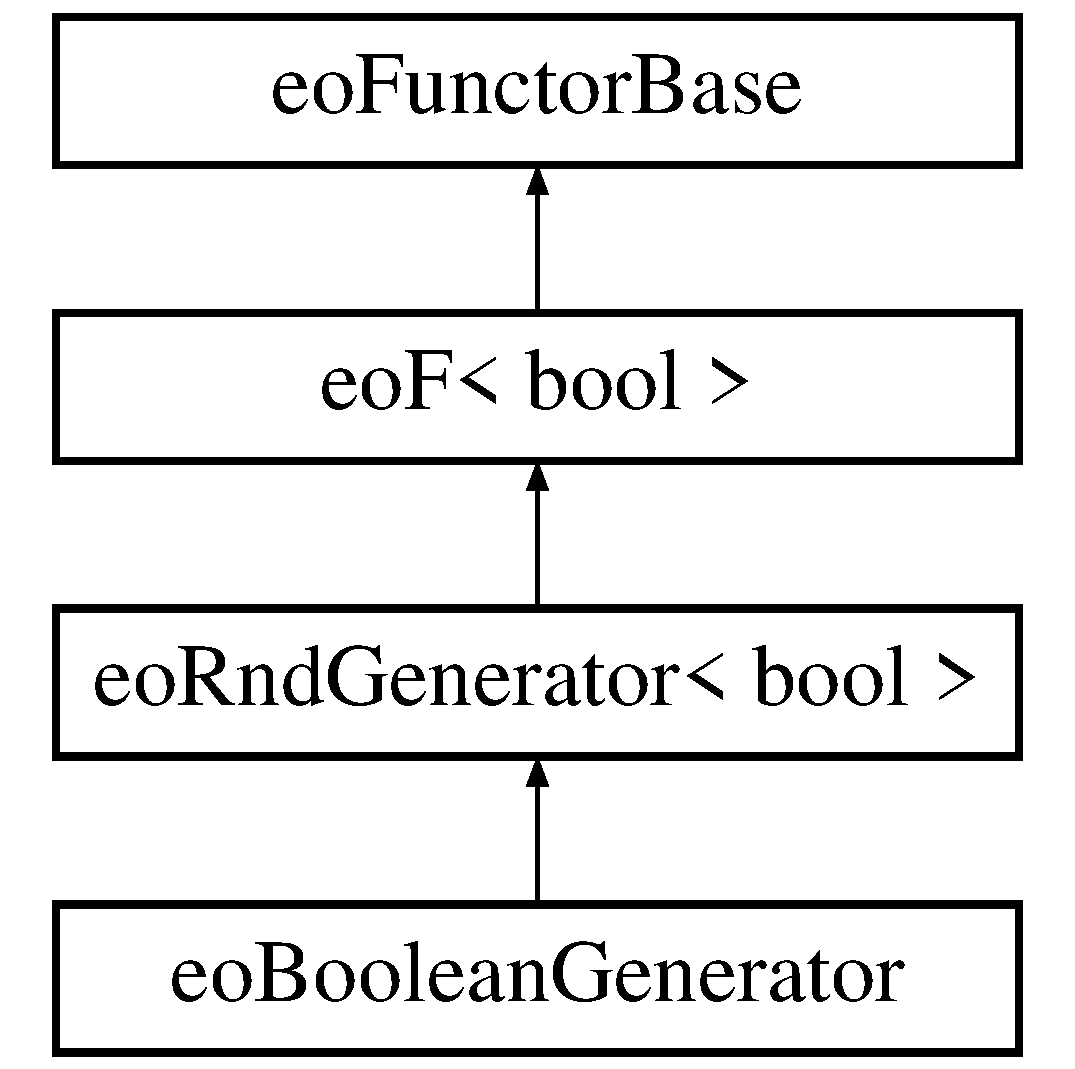
\includegraphics[height=4cm]{classeo_boolean_generator}
\end{center}
\end{figure}
\subsection*{Public Member Functions}
\begin{CompactItemize}
\item 
{\bf eo\-Boolean\-Generator} (float \_\-bias=0.5, {\bf eo\-Rng} \&\_\-rng=rng)\label{classeo_boolean_generator_a0}

\item 
bool {\bf operator()} (void)\label{classeo_boolean_generator_a1}

\begin{CompactList}\small\item\em The pure virtual function that needs to be implemented by the subclass. \item\end{CompactList}\end{CompactItemize}
\subsection*{Private Attributes}
\begin{CompactItemize}
\item 
float {\bf bias}\label{classeo_boolean_generator_r0}

\item 
{\bf eo\-Rng} \& {\bf gen}\label{classeo_boolean_generator_r1}

\end{CompactItemize}


\subsection{Detailed Description}
The class eo\-Boolean\-Generator can be used in the STL generate function to easily generate random booleans with a specified bias. 



Definition at line 104 of file eo\-Rnd\-Generators.h.

The documentation for this class was generated from the following file:\begin{CompactItemize}
\item 
eo\-Rnd\-Generators.h\end{CompactItemize}

\section{eo\-Boolean\-Init Class Reference}
\label{classeo_boolean_init}\index{eoBooleanInit@{eoBooleanInit}}
The class eo\-Boolean\-Init can be used in the STL apply function to easily generate random booleans with a specified bias.  


{\tt \#include $<$eo\-Uniform\-Init.h$>$}

Inheritance diagram for eo\-Boolean\-Init::\begin{figure}[H]
\begin{center}
\leavevmode
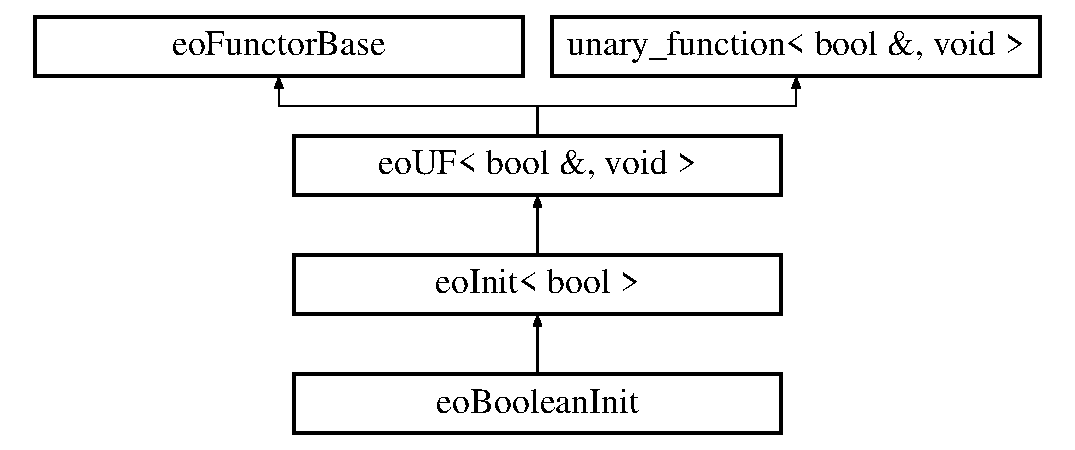
\includegraphics[height=4cm]{classeo_boolean_init}
\end{center}
\end{figure}
\subsection*{Public Member Functions}
\begin{CompactItemize}
\item 
{\bf eo\-Boolean\-Init} (float \_\-bias=0.5, {\bf eo\-Rng} \&\_\-rng=rng)\label{classeo_boolean_init_a0}

\item 
void {\bf operator()} (bool \&\_\-b)\label{classeo_boolean_init_a1}

\begin{CompactList}\small\item\em The pure virtual function that needs to be implemented by the subclass. \item\end{CompactList}\end{CompactItemize}
\subsection*{Private Attributes}
\begin{CompactItemize}
\item 
float {\bf bias}\label{classeo_boolean_init_r0}

\item 
{\bf eo\-Rng} \& {\bf gen}\label{classeo_boolean_init_r1}

\end{CompactItemize}


\subsection{Detailed Description}
The class eo\-Boolean\-Init can be used in the STL apply function to easily generate random booleans with a specified bias. 



Definition at line 110 of file eo\-Uniform\-Init.h.

The documentation for this class was generated from the following file:\begin{CompactItemize}
\item 
eo\-Uniform\-Init.h\end{CompactItemize}

\section{eo\-Bool\-Flip Class Reference}
\label{classeo_bool_flip}\index{eoBoolFlip@{eoBoolFlip}}
a simple boolean mutation - to be used in generic eo\-Op's  


{\tt \#include $<$eo\-Bool\-Flip.h$>$}

Inheritance diagram for eo\-Bool\-Flip::\begin{figure}[H]
\begin{center}
\leavevmode
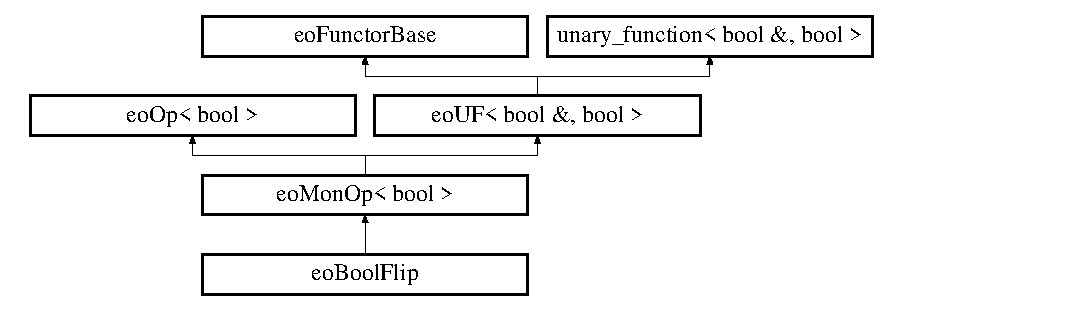
\includegraphics[height=3.73333cm]{classeo_bool_flip}
\end{center}
\end{figure}
\subsection*{Public Member Functions}
\begin{CompactItemize}
\item 
bool {\bf operator()} (bool \&\_\-b)\label{classeo_bool_flip_a0}

\begin{CompactList}\small\item\em simply flips the boolean argument \item\end{CompactList}\item 
virtual string {\bf class\-Name} () const \label{classeo_bool_flip_a1}

\begin{CompactList}\small\item\em inherited {\bf class\-Name()}{\rm (p.\,\pageref{classeo_bool_flip_a1})} \item\end{CompactList}\end{CompactItemize}


\subsection{Detailed Description}
a simple boolean mutation - to be used in generic eo\-Op's 



Definition at line 32 of file eo\-Bool\-Flip.h.

The documentation for this class was generated from the following file:\begin{CompactItemize}
\item 
eo\-Bool\-Flip.h\end{CompactItemize}

\section{eo\-Branch\-Mutation$<$ FType, Node $>$ Class Template Reference}
\label{classeo_branch_mutation}\index{eoBranchMutation@{eoBranchMutation}}
eo\-Branch\-Mutation --$>$ replace a subtree with a randomly created subtree  


{\tt \#include $<$gp/eo\-Parse\-Tree\-Op.h$>$}

Inheritance diagram for eo\-Branch\-Mutation$<$ FType, Node $>$::\begin{figure}[H]
\begin{center}
\leavevmode
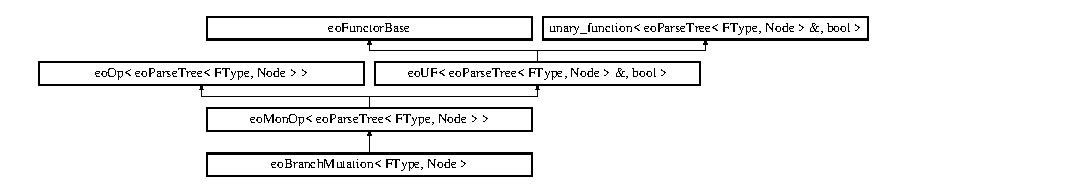
\includegraphics[height=2.14559cm]{classeo_branch_mutation}
\end{center}
\end{figure}
\subsection*{Public Types}
\begin{CompactItemize}
\item 
typedef {\bf eo\-Parse\-Tree}$<$ FType, Node $>$ {\bf Eo\-Type}\label{classeo_branch_mutation_w0}

\end{CompactItemize}
\subsection*{Public Member Functions}
\begin{CompactItemize}
\item 
{\bf eo\-Branch\-Mutation} ({\bf eo\-Init}$<$ {\bf Eo\-Type} $>$ \&\_\-init, unsigned \_\-max\_\-length)
\begin{CompactList}\small\item\em Constructor. \item\end{CompactList}\item 
virtual std::string {\bf class\-Name} () const \label{classeo_branch_mutation_a1}

\begin{CompactList}\small\item\em the class name \item\end{CompactList}\item 
virtual {\bf $\sim$eo\-Branch\-Mutation} ()\label{classeo_branch_mutation_a2}

\begin{CompactList}\small\item\em Dtor. \item\end{CompactList}\item 
bool {\bf operator()} ({\bf Eo\-Type} \&\_\-eo1)
\begin{CompactList}\small\item\em Mutate an individual. \item\end{CompactList}\end{CompactItemize}
\subsection*{Private Attributes}
\begin{CompactItemize}
\item 
unsigned {\bf max\_\-length}\label{classeo_branch_mutation_r0}

\item 
{\bf eo\-Init}$<$ {\bf Eo\-Type} $>$ \& {\bf initializer}\label{classeo_branch_mutation_r1}

\end{CompactItemize}


\subsection{Detailed Description}
\subsubsection*{template$<$class FType, class Node$>$ class eo\-Branch\-Mutation$<$ FType, Node $>$}

eo\-Branch\-Mutation --$>$ replace a subtree with a randomly created subtree 



Definition at line 87 of file eo\-Parse\-Tree\-Op.h.

\subsection{Constructor \& Destructor Documentation}
\index{eoBranchMutation@{eo\-Branch\-Mutation}!eoBranchMutation@{eoBranchMutation}}
\index{eoBranchMutation@{eoBranchMutation}!eoBranchMutation@{eo\-Branch\-Mutation}}
\subsubsection{\setlength{\rightskip}{0pt plus 5cm}template$<$class FType, class Node$>$ {\bf eo\-Branch\-Mutation}$<$ FType, Node $>$::{\bf eo\-Branch\-Mutation} ({\bf eo\-Init}$<$ {\bf Eo\-Type} $>$ \& {\em \_\-init}, unsigned {\em \_\-max\_\-length})\hspace{0.3cm}{\tt  [inline]}}\label{classeo_branch_mutation_a0}


Constructor. 

\begin{Desc}
\item[Parameters:]
\begin{description}
\item[{\em \_\-init}]An instantiation of eo\-Gp\-Depth\-Initializer \item[{\em \_\-max\_\-length}]the maximum size of an individual \end{description}
\end{Desc}


Definition at line 97 of file eo\-Parse\-Tree\-Op.h.

\subsection{Member Function Documentation}
\index{eoBranchMutation@{eo\-Branch\-Mutation}!operator()@{operator()}}
\index{operator()@{operator()}!eoBranchMutation@{eo\-Branch\-Mutation}}
\subsubsection{\setlength{\rightskip}{0pt plus 5cm}template$<$class FType, class Node$>$ bool {\bf eo\-Branch\-Mutation}$<$ FType, Node $>$::operator() ({\bf Eo\-Type} \& {\em \_\-eo1})\hspace{0.3cm}{\tt  [inline]}}\label{classeo_branch_mutation_a3}


Mutate an individual. 

\begin{Desc}
\item[Parameters:]
\begin{description}
\item[{\em \_\-eo1}]The individual that is to be changed \end{description}
\end{Desc}


Definition at line 111 of file eo\-Parse\-Tree\-Op.h.

References eo\-Parse\-Tree$<$ FType, Node $>$::prune\-Tree(), and eo\-Rng::random().

The documentation for this class was generated from the following file:\begin{CompactItemize}
\item 
eo\-Parse\-Tree\-Op.h\end{CompactItemize}

\section{eo\-Breed$<$ EOT $>$ Class Template Reference}
\label{classeo_breed}\index{eoBreed@{eoBreed}}
Breeding: combination of selecting and transforming a population.  


{\tt \#include $<$eo\-Breed.h$>$}

Inheritance diagram for eo\-Breed$<$ EOT $>$::\begin{figure}[H]
\begin{center}
\leavevmode
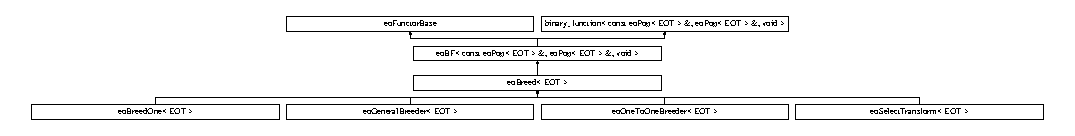
\includegraphics[height=1.37592cm]{classeo_breed}
\end{center}
\end{figure}


\subsection{Detailed Description}
\subsubsection*{template$<$class EOT$>$ class eo\-Breed$<$ EOT $>$}

Breeding: combination of selecting and transforming a population. 

Breeding is thought of a combination of selecting and transforming a population. For efficiency reasons you might want to build your own eo\-Breed derived class rather than relying on a seperate select and transform function.

\begin{Desc}
\item[See also:]{\bf eo\-Select}{\rm (p.\,\pageref{classeo_select})}, {\bf eo\-Transform}{\rm (p.\,\pageref{classeo_transform})}, {\bf eo\-Select\-Transform}{\rm (p.\,\pageref{classeo_select_transform})} \end{Desc}




Definition at line 46 of file eo\-Breed.h.

The documentation for this class was generated from the following file:\begin{CompactItemize}
\item 
eo\-Breed.h\end{CompactItemize}

\section{eo\-Cellular\-Easy\-EA$<$ EOT $>$ Class Template Reference}
\label{classeo_cellular_easy_e_a}\index{eoCellularEasyEA@{eoCellularEasyEA}}
The abstract cellular easy algorithm.  


{\tt \#include $<$eo\-Cellular\-Easy\-EA.h$>$}

Inheritance diagram for eo\-Cellular\-Easy\-EA$<$ EOT $>$::\begin{figure}[H]
\begin{center}
\leavevmode
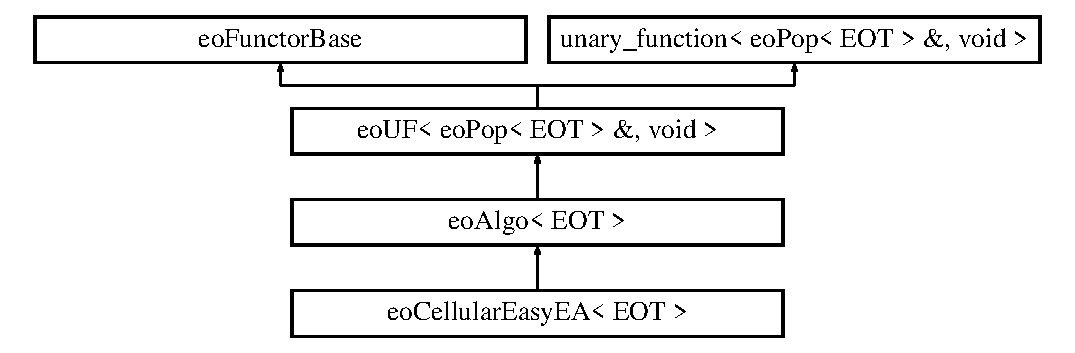
\includegraphics[height=4cm]{classeo_cellular_easy_e_a}
\end{center}
\end{figure}
\subsection*{Public Member Functions}
\begin{CompactItemize}
\item 
{\bf eo\-Cellular\-Easy\-EA} ({\bf eo\-Continue}$<$ {\bf EOT} $>$ \&\_\-cont, {\bf eo\-Eval\-Func}$<$ {\bf EOT} $>$ \&\_\-eval, {\bf eo\-Select\-One}$<$ {\bf EOT} $>$ \&\_\-sel\_\-neigh, {\bf eo\-Bin\-Op}$<$ {\bf EOT} $>$ \&\_\-cross, {\bf eo\-Mon\-Op}$<$ {\bf EOT} $>$ \&\_\-mut, {\bf eo\-Select\-One}$<$ {\bf EOT} $>$ \&\_\-sel\_\-repl)\label{classeo_cellular_easy_e_a_a0}

\begin{CompactList}\small\item\em Two constructors. \item\end{CompactList}\item 
{\bf eo\-Cellular\-Easy\-EA} ({\bf eo\-Continue}$<$ {\bf EOT} $>$ \&\_\-cont, {\bf eo\-Eval\-Func}$<$ {\bf EOT} $>$ \&\_\-eval, {\bf eo\-Select\-One}$<$ {\bf EOT} $>$ \&\_\-sel\_\-neigh, {\bf eo\-Quad\-Op}$<$ {\bf EOT} $>$ \&\_\-cross, {\bf eo\-Mon\-Op}$<$ {\bf EOT} $>$ \&\_\-mut, {\bf eo\-Select\-One}$<$ {\bf EOT} $>$ \&\_\-sel\_\-child, {\bf eo\-Select\-One}$<$ {\bf EOT} $>$ \&\_\-sel\_\-repl)\label{classeo_cellular_easy_e_a_a1}

\item 
void {\bf operator()} ({\bf eo\-Pop}$<$ {\bf EOT} $>$ \&pop)\label{classeo_cellular_easy_e_a_a2}

\begin{CompactList}\small\item\em For a given population. \item\end{CompactList}\end{CompactItemize}
\subsection*{Protected Member Functions}
\begin{CompactItemize}
\item 
virtual {\bf eo\-Pop}$<$ {\bf EOT} $>$ {\bf neighbours} (const {\bf eo\-Pop}$<$ {\bf EOT} $>$ \&pop, int rank)=0\label{classeo_cellular_easy_e_a_b0}

\end{CompactItemize}
\subsection*{Private Attributes}
\begin{CompactItemize}
\item 
{\bf eo\-Continue}$<$ {\bf EOT} $>$ \& {\bf cont}\label{classeo_cellular_easy_e_a_r0}

\item 
{\bf eo\-Eval\-Func}$<$ {\bf EOT} $>$ \& {\bf eval}\label{classeo_cellular_easy_e_a_r1}

\item 
{\bf eo\-Pop\-Loop\-Eval}$<$ {\bf EOT} $>$ {\bf pop\-Eval}\label{classeo_cellular_easy_e_a_r2}

\item 
{\bf eo\-Select\-One}$<$ {\bf EOT} $>$ \& {\bf sel\_\-neigh}\label{classeo_cellular_easy_e_a_r3}

\item 
{\bf eo\-BF}$<$ {\bf EOT} \&, {\bf EOT} \&, bool $>$ \& {\bf cross}\label{classeo_cellular_easy_e_a_r4}

\item 
{\bf eo\-Mon\-Op}$<$ {\bf EOT} $>$ \& {\bf mut}\label{classeo_cellular_easy_e_a_r5}

\item 
{\bf eo\-Select\-One}$<$ {\bf EOT} $>$ \& {\bf sel\_\-child}\label{classeo_cellular_easy_e_a_r6}

\item 
{\bf eo\-Select\-One}$<$ {\bf EOT} $>$ \& {\bf sel\_\-repl}\label{classeo_cellular_easy_e_a_r7}

\end{CompactItemize}


\subsection{Detailed Description}
\subsubsection*{template$<$class EOT$>$ class eo\-Cellular\-Easy\-EA$<$ EOT $>$}

The abstract cellular easy algorithm. 



Definition at line 38 of file eo\-Cellular\-Easy\-EA.h.

The documentation for this class was generated from the following file:\begin{CompactItemize}
\item 
eo\-Cellular\-Easy\-EA.h\end{CompactItemize}

\section{eo\-Check\-Point$<$ EOT $>$ Class Template Reference}
\label{classeo_check_point}\index{eoCheckPoint@{eoCheckPoint}}
eo\-Check\-Point is a container class.  


{\tt \#include $<$eo\-Check\-Point.h$>$}

Inheritance diagram for eo\-Check\-Point$<$ EOT $>$::\begin{figure}[H]
\begin{center}
\leavevmode
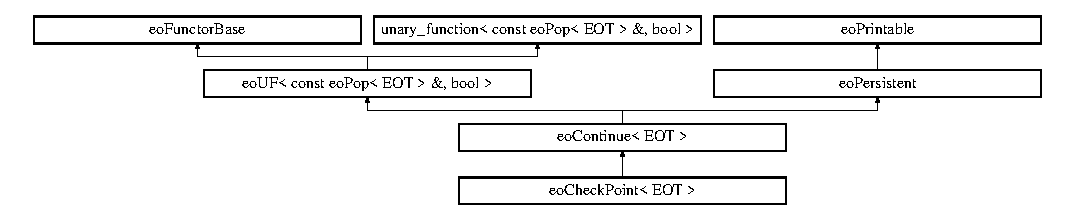
\includegraphics[height=2.52252cm]{classeo_check_point}
\end{center}
\end{figure}
\subsection*{Public Member Functions}
\begin{CompactItemize}
\item 
{\bf eo\-Check\-Point} ({\bf eo\-Continue}$<$ {\bf EOT} $>$ \&\_\-cont)\label{classeo_check_point_a0}

\item 
bool {\bf operator()} (const {\bf eo\-Pop}$<$ {\bf EOT} $>$ \&\_\-pop)\label{classeo_check_point_a1}

\begin{CompactList}\small\item\em The pure virtual function that needs to be implemented by the subclass. \item\end{CompactList}\item 
void {\bf add} ({\bf eo\-Continue}$<$ {\bf EOT} $>$ \&\_\-cont)\label{classeo_check_point_a2}

\item 
void {\bf add} ({\bf eo\-Sorted\-Stat\-Base}$<$ {\bf EOT} $>$ \&\_\-stat)\label{classeo_check_point_a3}

\item 
void {\bf add} ({\bf eo\-Stat\-Base}$<$ {\bf EOT} $>$ \&\_\-stat)\label{classeo_check_point_a4}

\item 
void {\bf add} ({\bf eo\-Monitor} \&\_\-mon)\label{classeo_check_point_a5}

\item 
void {\bf add} ({\bf eo\-Updater} \&\_\-upd)\label{classeo_check_point_a6}

\item 
virtual std::string {\bf class\-Name} (void) const \label{classeo_check_point_a7}

\item 
std::string {\bf all\-Class\-Names} () const \label{classeo_check_point_a8}

\begin{CompactList}\small\item\em returns a string with all class\-Name() of data separated with \char`\"{}$\backslash$n\char`\"{} (for debugging) \item\end{CompactList}\end{CompactItemize}
\subsection*{Private Attributes}
\begin{CompactItemize}
\item 
std::vector$<$ {\bf eo\-Continue}$<$ {\bf EOT} $>$ $\ast$ $>$ {\bf continuators}\label{classeo_check_point_r0}

\item 
std::vector$<$ {\bf eo\-Sorted\-Stat\-Base}$<$ {\bf EOT} $>$ $\ast$ $>$ {\bf sorted}\label{classeo_check_point_r1}

\item 
std::vector$<$ {\bf eo\-Stat\-Base}$<$ {\bf EOT} $>$ $\ast$ $>$ {\bf stats}\label{classeo_check_point_r2}

\item 
std::vector$<$ {\bf eo\-Monitor} $\ast$ $>$ {\bf monitors}\label{classeo_check_point_r3}

\item 
std::vector$<$ {\bf eo\-Updater} $\ast$ $>$ {\bf updaters}\label{classeo_check_point_r4}

\end{CompactItemize}


\subsection{Detailed Description}
\subsubsection*{template$<$class EOT$>$ class eo\-Check\-Point$<$ EOT $>$}

eo\-Check\-Point is a container class. 

It contains std::vectors of (pointers to) {\bf eo\-Continue}{\rm (p.\,\pageref{classeo_continue})} (modif. MS July 16. 2002) eo\-Stats, {\bf eo\-Updater}{\rm (p.\,\pageref{classeo_updater})} and {\bf eo\-Monitor}{\rm (p.\,\pageref{classeo_monitor})} it is an {\bf eo\-Continue}{\rm (p.\,\pageref{classeo_continue})}, so its operator() will be called every generation - and will return the contained-combined-eo\-Continue result but before that it will call in turn every single \{statistics, updaters, monitors\} that it has been given, and after that, if stopping, all last\-Call methods of the above. 



Definition at line 46 of file eo\-Check\-Point.h.

The documentation for this class was generated from the following file:\begin{CompactItemize}
\item 
eo\-Check\-Point.h\end{CompactItemize}

\section{eo\-CMABreed$<$ Fit\-T $>$ Class Template Reference}
\label{classeo_c_m_a_breed}\index{eoCMABreed@{eoCMABreed}}
TODO, handle bounds.  


{\tt \#include $<$eo\-CMABreed.h$>$}

Inheritance diagram for eo\-CMABreed$<$ Fit\-T $>$::\begin{figure}[H]
\begin{center}
\leavevmode
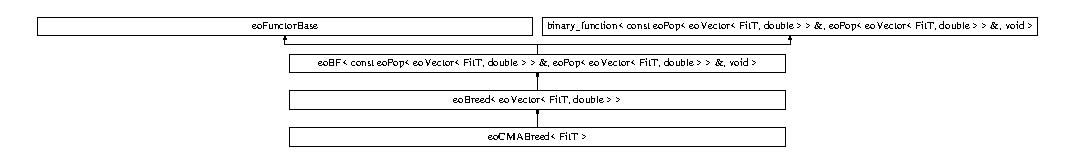
\includegraphics[height=1.73643cm]{classeo_c_m_a_breed}
\end{center}
\end{figure}
\subsection*{Public Member Functions}
\begin{CompactItemize}
\item 
{\bf eo\-CMABreed} (eo::CMAState \&state\_\-, unsigned lambda\_\-)\label{classeo_c_m_a_breed_a0}

\item 
void {\bf operator()} (const {\bf eo\-Pop}$<$ {\bf EOT} $>$ \&parents, {\bf eo\-Pop}$<$ {\bf EOT} $>$ \&offspring)\label{classeo_c_m_a_breed_a1}

\end{CompactItemize}
\subsection*{Private Types}
\begin{CompactItemize}
\item 
typedef {\bf eo\-Vector}$<$ {\bf Fit\-T}, double $>$ {\bf EOT}\label{classeo_c_m_a_breed_y0}

\end{CompactItemize}
\subsection*{Private Attributes}
\begin{CompactItemize}
\item 
eo::CMAState \& {\bf state}\label{classeo_c_m_a_breed_r0}

\item 
unsigned {\bf lambda}\label{classeo_c_m_a_breed_r1}

\end{CompactItemize}


\subsection{Detailed Description}
\subsubsection*{template$<$class Fit\-T$>$ class eo\-CMABreed$<$ Fit\-T $>$}

TODO, handle bounds. 



Definition at line 36 of file eo\-CMABreed.h.

The documentation for this class was generated from the following file:\begin{CompactItemize}
\item 
eo\-CMABreed.h\end{CompactItemize}

\section{eo\-CMAInit$<$ Fit\-T $>$ Class Template Reference}
\label{classeo_c_m_a_init}\index{eoCMAInit@{eoCMAInit}}
TODO, handle bounds.  


{\tt \#include $<$eo\-CMAInit.h$>$}

Inheritance diagram for eo\-CMAInit$<$ Fit\-T $>$::\begin{figure}[H]
\begin{center}
\leavevmode
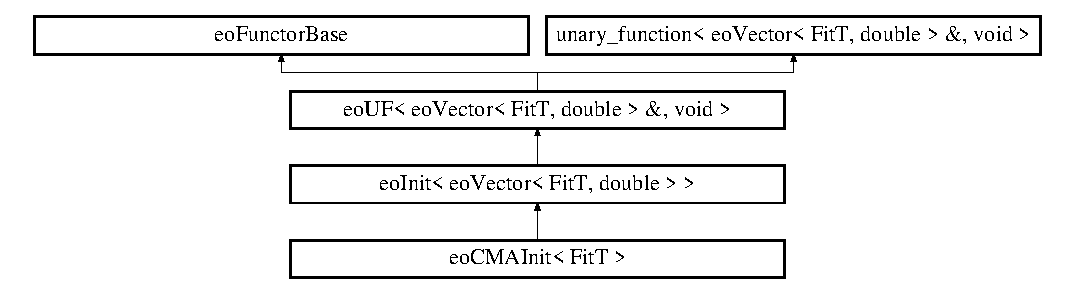
\includegraphics[height=3.5cm]{classeo_c_m_a_init}
\end{center}
\end{figure}
\subsection*{Public Member Functions}
\begin{CompactItemize}
\item 
{\bf eo\-CMAInit} (const eo::CMAState \&state\_\-)\label{classeo_c_m_a_init_a0}

\item 
void {\bf operator()} ({\bf EOT} \&v)\label{classeo_c_m_a_init_a1}

\end{CompactItemize}
\subsection*{Private Types}
\begin{CompactItemize}
\item 
typedef {\bf eo\-Vector}$<$ {\bf Fit\-T}, double $>$ {\bf EOT}\label{classeo_c_m_a_init_y0}

\end{CompactItemize}
\subsection*{Private Attributes}
\begin{CompactItemize}
\item 
const eo::CMAState \& {\bf state}\label{classeo_c_m_a_init_r0}

\end{CompactItemize}


\subsection{Detailed Description}
\subsubsection*{template$<$class Fit\-T$>$ class eo\-CMAInit$<$ Fit\-T $>$}

TODO, handle bounds. 



Definition at line 37 of file eo\-CMAInit.h.

The documentation for this class was generated from the following file:\begin{CompactItemize}
\item 
eo\-CMAInit.h\end{CompactItemize}

\section{eo\-Collapse\-Subtree\-Mutation$<$ FType, Node $>$ Class Template Reference}
\label{classeo_collapse_subtree_mutation}\index{eoCollapseSubtreeMutation@{eoCollapseSubtreeMutation}}
eo\-Collapse\-Subtree --$>$ replace a subtree with a randomly chosen terminal  


{\tt \#include $<$gp/eo\-Parse\-Tree\-Op.h$>$}

Inheritance diagram for eo\-Collapse\-Subtree\-Mutation$<$ FType, Node $>$::\begin{figure}[H]
\begin{center}
\leavevmode
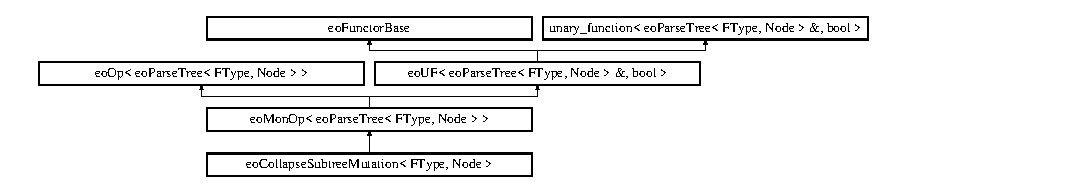
\includegraphics[height=2.14559cm]{classeo_collapse_subtree_mutation}
\end{center}
\end{figure}
\subsection*{Public Types}
\begin{CompactItemize}
\item 
typedef {\bf eo\-Parse\-Tree}$<$ FType, Node $>$ {\bf Eo\-Type}\label{classeo_collapse_subtree_mutation_w0}

\end{CompactItemize}
\subsection*{Public Member Functions}
\begin{CompactItemize}
\item 
{\bf eo\-Collapse\-Subtree\-Mutation} ({\bf eo\-Init}$<$ {\bf Eo\-Type} $>$ \&\_\-init, unsigned \_\-max\_\-length)
\begin{CompactList}\small\item\em Constructor. \item\end{CompactList}\item 
virtual std::string {\bf class\-Name} () const \label{classeo_collapse_subtree_mutation_a1}

\begin{CompactList}\small\item\em The class name. \item\end{CompactList}\item 
virtual {\bf $\sim$eo\-Collapse\-Subtree\-Mutation} ()\label{classeo_collapse_subtree_mutation_a2}

\begin{CompactList}\small\item\em Dtor. \item\end{CompactList}\item 
bool {\bf operator()} ({\bf Eo\-Type} \&\_\-eo1)
\begin{CompactList}\small\item\em Mutate an individual. \item\end{CompactList}\end{CompactItemize}
\subsection*{Private Attributes}
\begin{CompactItemize}
\item 
unsigned {\bf max\_\-length}\label{classeo_collapse_subtree_mutation_r0}

\item 
{\bf eo\-Init}$<$ {\bf Eo\-Type} $>$ \& {\bf initializer}\label{classeo_collapse_subtree_mutation_r1}

\end{CompactItemize}


\subsection{Detailed Description}
\subsubsection*{template$<$class FType, class Node$>$ class eo\-Collapse\-Subtree\-Mutation$<$ FType, Node $>$}

eo\-Collapse\-Subtree --$>$ replace a subtree with a randomly chosen terminal 



Definition at line 272 of file eo\-Parse\-Tree\-Op.h.

\subsection{Constructor \& Destructor Documentation}
\index{eoCollapseSubtreeMutation@{eo\-Collapse\-Subtree\-Mutation}!eoCollapseSubtreeMutation@{eoCollapseSubtreeMutation}}
\index{eoCollapseSubtreeMutation@{eoCollapseSubtreeMutation}!eoCollapseSubtreeMutation@{eo\-Collapse\-Subtree\-Mutation}}
\subsubsection{\setlength{\rightskip}{0pt plus 5cm}template$<$class FType, class Node$>$ {\bf eo\-Collapse\-Subtree\-Mutation}$<$ FType, Node $>$::{\bf eo\-Collapse\-Subtree\-Mutation} ({\bf eo\-Init}$<$ {\bf Eo\-Type} $>$ \& {\em \_\-init}, unsigned {\em \_\-max\_\-length})\hspace{0.3cm}{\tt  [inline]}}\label{classeo_collapse_subtree_mutation_a0}


Constructor. 

\begin{Desc}
\item[Parameters:]
\begin{description}
\item[{\em \_\-init}]An instantiation of eo\-Gp\-Depth\-Initializer \item[{\em \_\-max\_\-length}]the maximum size of an individual \end{description}
\end{Desc}


Definition at line 282 of file eo\-Parse\-Tree\-Op.h.

\subsection{Member Function Documentation}
\index{eoCollapseSubtreeMutation@{eo\-Collapse\-Subtree\-Mutation}!operator()@{operator()}}
\index{operator()@{operator()}!eoCollapseSubtreeMutation@{eo\-Collapse\-Subtree\-Mutation}}
\subsubsection{\setlength{\rightskip}{0pt plus 5cm}template$<$class FType, class Node$>$ bool {\bf eo\-Collapse\-Subtree\-Mutation}$<$ FType, Node $>$::operator() ({\bf Eo\-Type} \& {\em \_\-eo1})\hspace{0.3cm}{\tt  [inline]}}\label{classeo_collapse_subtree_mutation_a3}


Mutate an individual. 

\begin{Desc}
\item[Parameters:]
\begin{description}
\item[{\em \_\-eo1}]The individual that is to be changed \end{description}
\end{Desc}


Definition at line 295 of file eo\-Parse\-Tree\-Op.h.

References eo\-Parse\-Tree$<$ FType, Node $>$::prune\-Tree(), and eo\-Rng::random().

The documentation for this class was generated from the following file:\begin{CompactItemize}
\item 
eo\-Parse\-Tree\-Op.h\end{CompactItemize}

\section{eo\-Combined\-Continue$<$ EOT $>$ Class Template Reference}
\label{classeo_combined_continue}\index{eoCombinedContinue@{eoCombinedContinue}}
Combined continuators - logical AND: Continues until one of the embedded continuators says halt!  


{\tt \#include $<$eo\-Combined\-Continue.h$>$}

Inheritance diagram for eo\-Combined\-Continue$<$ EOT $>$::\begin{figure}[H]
\begin{center}
\leavevmode
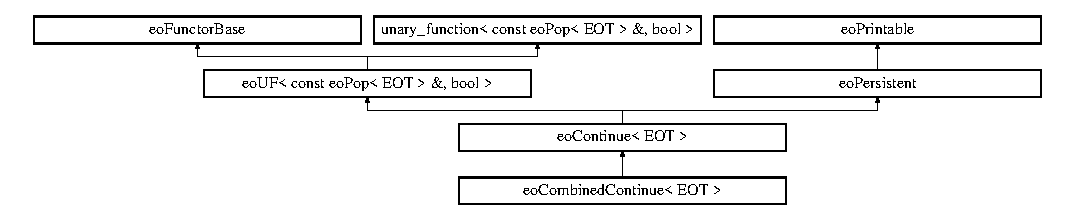
\includegraphics[height=2.52252cm]{classeo_combined_continue}
\end{center}
\end{figure}
\subsection*{Public Types}
\begin{CompactItemize}
\item 
typedef EOT::Fitness {\bf Fitness\-Type}\label{classeo_combined_continue_w0}

\begin{CompactList}\small\item\em Define Fitness. \item\end{CompactList}\end{CompactItemize}
\subsection*{Public Member Functions}
\begin{CompactItemize}
\item 
{\bf eo\-Combined\-Continue} ({\bf eo\-Continue}$<$ {\bf EOT} $>$ \&\_\-cont)\label{classeo_combined_continue_a0}

\begin{CompactList}\small\item\em Ctor, make sure that at least on continuator is present. \item\end{CompactList}\item 
{\bf eo\-Combined\-Continue} ({\bf eo\-Continue}$<$ {\bf EOT} $>$ \&\_\-cont1, {\bf eo\-Continue}$<$ {\bf EOT} $>$ \&\_\-cont2)\label{classeo_combined_continue_a1}

\begin{CompactList}\small\item\em Ctor - for historical reasons ... should disspear some day. \item\end{CompactList}\item 
void {\bf add} ({\bf eo\-Continue}$<$ {\bf EOT} $>$ \&\_\-cont)\label{classeo_combined_continue_a2}

\item 
void {\bf remove\-Last} (void)\label{classeo_combined_continue_a3}

\item 
virtual bool {\bf operator()} (const {\bf eo\-Pop}$<$ {\bf EOT} $>$ \&\_\-pop)\label{classeo_combined_continue_a4}

\begin{CompactList}\small\item\em Returns false when one of the embedded continuators say so (logical and). \item\end{CompactList}\item 
virtual std::string {\bf class\-Name} (void) const \label{classeo_combined_continue_a5}

\end{CompactItemize}
\subsection*{Private Attributes}
\begin{CompactItemize}
\item 
std::vector$<$ {\bf eo\-Continue}$<$ {\bf EOT} $>$ $\ast$ $>$ {\bf continuators}\label{classeo_combined_continue_r0}

\end{CompactItemize}


\subsection{Detailed Description}
\subsubsection*{template$<$class EOT$>$ class eo\-Combined\-Continue$<$ EOT $>$}

Combined continuators - logical AND: Continues until one of the embedded continuators says halt! 

20/11/00 MS: Changed the 2-continuator construct to a std::vector$<$eo\-Continue$<$EOT$>$ $>$ to be consistent with other Combined constructs and allow to easily handle more than 2 continuators

02/2003 Ram\'{o}n Casero Ca\~{n}as - added the remove\-Last() method 



Definition at line 42 of file eo\-Combined\-Continue.h.

The documentation for this class was generated from the following file:\begin{CompactItemize}
\item 
eo\-Combined\-Continue.h\end{CompactItemize}

\section{eo\-Combined\-Init$<$ EOT $>$ Class Template Reference}
\label{classeo_combined_init}\index{eoCombinedInit@{eoCombinedInit}}
Combined INIT: a proportional recombination of {\bf eo\-Init}{\rm (p.\,\pageref{classeo_init})} objects.  


{\tt \#include $<$eo\-Combined\-Init.h$>$}

Inheritance diagram for eo\-Combined\-Init$<$ EOT $>$::\begin{figure}[H]
\begin{center}
\leavevmode
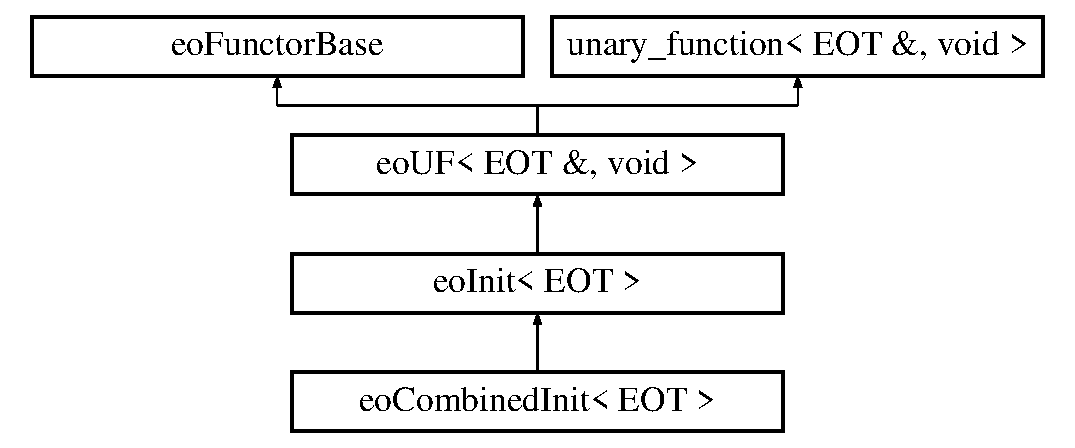
\includegraphics[height=4cm]{classeo_combined_init}
\end{center}
\end{figure}
\subsection*{Public Member Functions}
\begin{CompactItemize}
\item 
{\bf eo\-Combined\-Init} ({\bf eo\-Init}$<$ {\bf EOT} $>$ \&\_\-init, double \_\-rate)\label{classeo_combined_init_a0}

\begin{CompactList}\small\item\em Ctor, make sure that at least one {\bf eo\-Init}{\rm (p.\,\pageref{classeo_init})} is present. \item\end{CompactList}\item 
void {\bf add} ({\bf eo\-Init}$<$ {\bf EOT} $>$ \&\_\-init, double \_\-rate, bool \_\-verbose=false)\label{classeo_combined_init_a1}

\begin{CompactList}\small\item\em The usual method to add objects to the combination note the \_\-verbose parameter, that allows to print what's inside the combination with scaled rates. \item\end{CompactList}\item 
virtual void {\bf print\-On} (std::ostream \&\_\-os)\label{classeo_combined_init_a2}

\begin{CompactList}\small\item\em outputs the operators and percentages \item\end{CompactList}\item 
virtual void {\bf operator()} ({\bf EOT} \&\_\-eo)\label{classeo_combined_init_a3}

\begin{CompactList}\small\item\em Performs the init: chooses among all initializers using roulette wheel on the rates. \item\end{CompactList}\item 
virtual std::string {\bf class\-Name} (void) const 
\begin{CompactList}\small\item\em class\-Name: Mandatory because of eo\-Combined\-Init. \item\end{CompactList}\end{CompactItemize}
\subsection*{Private Attributes}
\begin{CompactItemize}
\item 
std::vector$<$ {\bf eo\-Init}$<$ {\bf EOT} $>$ $\ast$ $>$ {\bf initializers}\label{classeo_combined_init_r0}

\item 
std::vector$<$ double $>$ {\bf rates}\label{classeo_combined_init_r1}

\end{CompactItemize}


\subsection{Detailed Description}
\subsubsection*{template$<$class EOT$>$ class eo\-Combined\-Init$<$ EOT $>$}

Combined INIT: a proportional recombination of {\bf eo\-Init}{\rm (p.\,\pageref{classeo_init})} objects. 



Definition at line 35 of file eo\-Combined\-Init.h.

\subsection{Member Function Documentation}
\index{eoCombinedInit@{eo\-Combined\-Init}!className@{className}}
\index{className@{className}!eoCombinedInit@{eo\-Combined\-Init}}
\subsubsection{\setlength{\rightskip}{0pt plus 5cm}template$<$class EOT$>$ virtual std::string {\bf eo\-Combined\-Init}$<$ {\bf EOT} $>$::class\-Name (void) const\hspace{0.3cm}{\tt  [inline, virtual]}}\label{classeo_combined_init_a4}


class\-Name: Mandatory because of eo\-Combined\-Init. 

SHould be pure virtual, but then we should go over the whole code to write the method for all derived classes ... MS 16/7/04 

Reimplemented from {\bf eo\-Init$<$ EOT $>$} {\rm (p.\,\pageref{classeo_init_a0})}.

Definition at line 81 of file eo\-Combined\-Init.h.

Referenced by eo\-Combined\-Init$<$ EOT $>$::print\-On().

The documentation for this class was generated from the following file:\begin{CompactItemize}
\item 
eo\-Combined\-Init.h\end{CompactItemize}

\section{eo\-Comma\-Replacement$<$ EOT $>$ Class Template Reference}
\label{classeo_comma_replacement}\index{eoCommaReplacement@{eoCommaReplacement}}
ES type of replacement strategy: ignore parents, truncate offspring.  


{\tt \#include $<$eo\-Merge\-Reduce.h$>$}

Inheritance diagram for eo\-Comma\-Replacement$<$ EOT $>$::\begin{figure}[H]
\begin{center}
\leavevmode
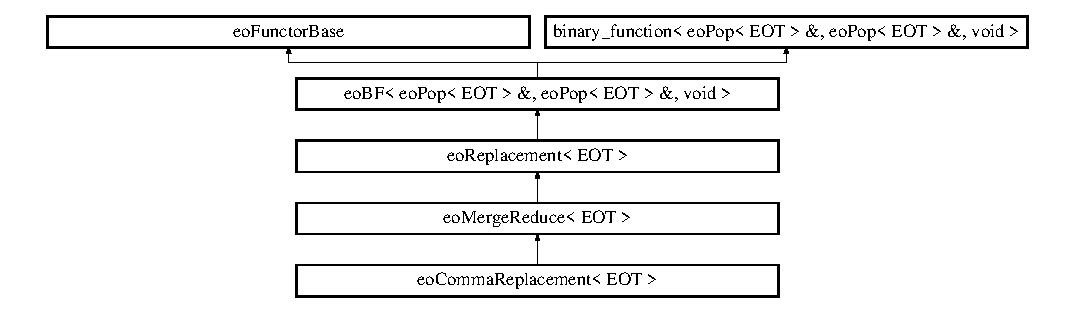
\includegraphics[height=3.76344cm]{classeo_comma_replacement}
\end{center}
\end{figure}
\subsection*{Private Attributes}
\begin{CompactItemize}
\item 
{\bf eo\-No\-Elitism}$<$ {\bf EOT} $>$ {\bf no\_\-elite}\label{classeo_comma_replacement_r0}

\item 
{\bf eo\-Truncate}$<$ {\bf EOT} $>$ {\bf truncate}\label{classeo_comma_replacement_r1}

\end{CompactItemize}


\subsection{Detailed Description}
\subsubsection*{template$<$class EOT$>$ class eo\-Comma\-Replacement$<$ EOT $>$}

ES type of replacement strategy: ignore parents, truncate offspring. 



Definition at line 87 of file eo\-Merge\-Reduce.h.

The documentation for this class was generated from the following file:\begin{CompactItemize}
\item 
eo\-Merge\-Reduce.h\end{CompactItemize}

\section{eo\-Continue$<$ EOT $>$ Class Template Reference}
\label{classeo_continue}\index{eoContinue@{eoContinue}}
Termination condition for the genetic algorithm Takes the population as input, returns true for continue, false for termination.  


{\tt \#include $<$eo\-Continue.h$>$}

Inheritance diagram for eo\-Continue$<$ EOT $>$::\begin{figure}[H]
\begin{center}
\leavevmode
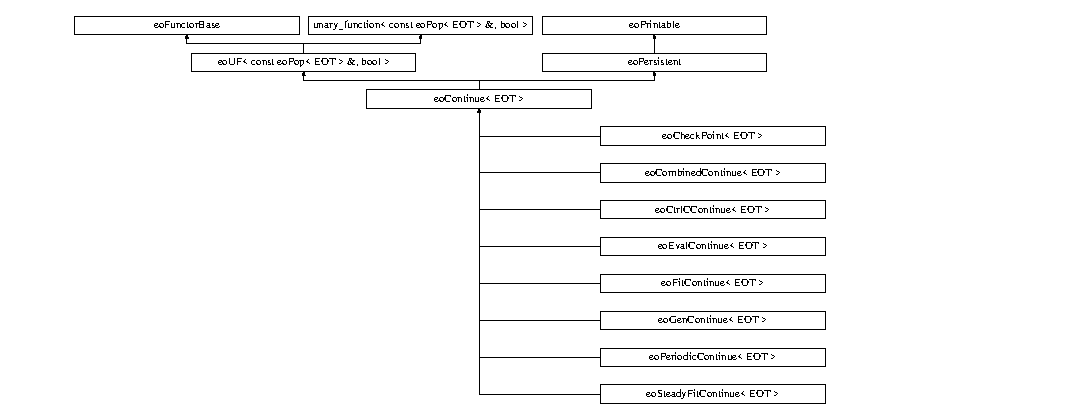
\includegraphics[height=5.2027cm]{classeo_continue}
\end{center}
\end{figure}
\subsection*{Public Member Functions}
\begin{CompactItemize}
\item 
virtual std::string {\bf class\-Name} (void) const \label{classeo_continue_a0}

\item 
void {\bf read\-From} (std::istream \&\_\-\_\-is)
\begin{CompactList}\small\item\em Read object. \item\end{CompactList}\item 
void {\bf print\-On} (std::ostream \&\_\-\_\-os) const 
\begin{CompactList}\small\item\em Write object. \item\end{CompactList}\end{CompactItemize}


\subsection{Detailed Description}
\subsubsection*{template$<$class EOT$>$ class eo\-Continue$<$ EOT $>$}

Termination condition for the genetic algorithm Takes the population as input, returns true for continue, false for termination. 



Definition at line 37 of file eo\-Continue.h.

\subsection{Member Function Documentation}
\index{eoContinue@{eo\-Continue}!readFrom@{readFrom}}
\index{readFrom@{readFrom}!eoContinue@{eo\-Continue}}
\subsubsection{\setlength{\rightskip}{0pt plus 5cm}template$<$class EOT$>$ void {\bf eo\-Continue}$<$ {\bf EOT} $>$::read\-From (std::istream \& {\em \_\-\_\-is})\hspace{0.3cm}{\tt  [inline, virtual]}}\label{classeo_continue_a1}


Read object. 

\begin{Desc}
\item[Parameters:]
\begin{description}
\item[{\em \_\-is}]A std::istream. \end{description}
\end{Desc}
\begin{Desc}
\item[Exceptions:]
\begin{description}
\item[{\em runtime\_\-std::exception}]If a valid object can't be read. \end{description}
\end{Desc}


Implements {\bf eo\-Persistent} {\rm (p.\,\pageref{classeo_persistent_a1})}.

Reimplemented in {\bf eo\-Gen\-Continue$<$ EOT $>$} {\rm (p.\,\pageref{classeo_gen_continue_a6})}.

Definition at line 42 of file eo\-Continue.h.\index{eoContinue@{eo\-Continue}!printOn@{printOn}}
\index{printOn@{printOn}!eoContinue@{eo\-Continue}}
\subsubsection{\setlength{\rightskip}{0pt plus 5cm}template$<$class EOT$>$ void {\bf eo\-Continue}$<$ {\bf EOT} $>$::print\-On (std::ostream \& {\em \_\-\_\-os}) const\hspace{0.3cm}{\tt  [inline, virtual]}}\label{classeo_continue_a2}


Write object. 

It's called print\-On since it prints the object on a stream. \begin{Desc}
\item[Parameters:]
\begin{description}
\item[{\em \_\-os}]A std::ostream. \end{description}
\end{Desc}


Implements {\bf eo\-Printable} {\rm (p.\,\pageref{classeo_printable_a1})}.

Reimplemented in {\bf eo\-Gen\-Continue$<$ EOT $>$} {\rm (p.\,\pageref{classeo_gen_continue_a7})}.

Definition at line 47 of file eo\-Continue.h.

The documentation for this class was generated from the following file:\begin{CompactItemize}
\item 
eo\-Continue.h\end{CompactItemize}

\section{eo\-Counted\-Dyn\-Update Class Reference}
\label{classeo_counted_dyn_update}\index{eoCountedDynUpdate@{eoCountedDynUpdate}}
An {\bf eo\-Updater}{\rm (p.\,\pageref{classeo_updater})} to update an {\bf eo\-Updatable}{\rm (p.\,\pageref{classeo_updatable})} object every given tic.  


{\tt \#include $<$eo\-Updatable.h$>$}

Inheritance diagram for eo\-Counted\-Dyn\-Update::\begin{figure}[H]
\begin{center}
\leavevmode
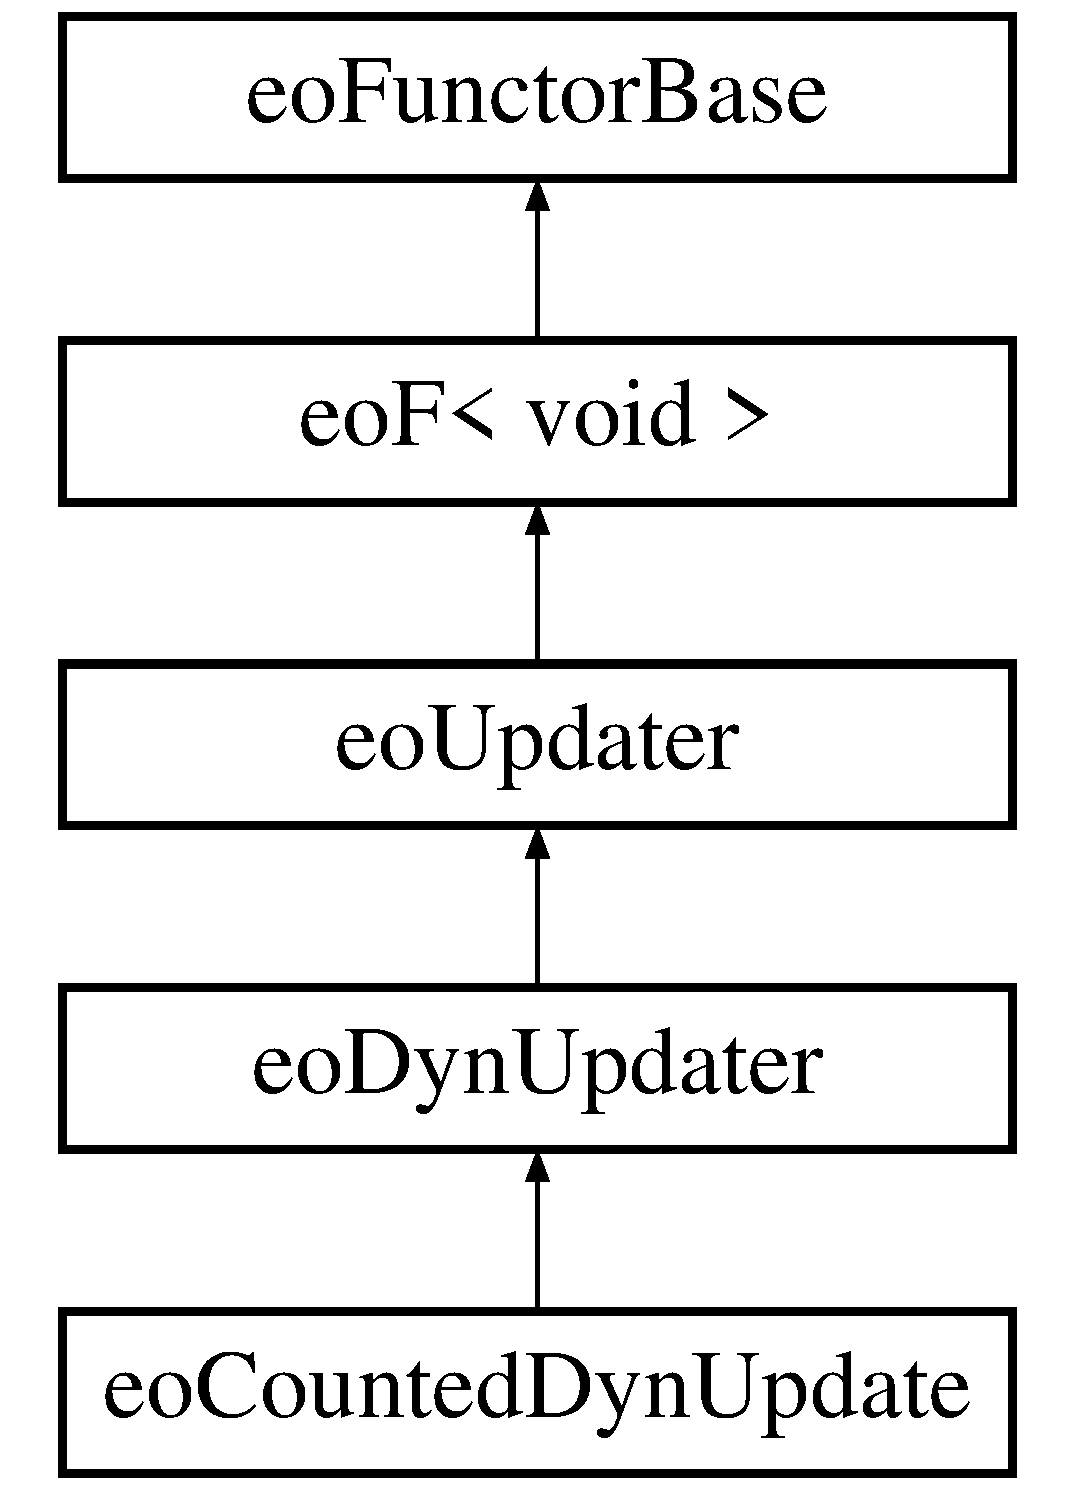
\includegraphics[height=5cm]{classeo_counted_dyn_update}
\end{center}
\end{figure}
\subsection*{Public Member Functions}
\begin{CompactItemize}
\item 
{\bf eo\-Counted\-Dyn\-Update} ({\bf eo\-Updatable} \&\_\-to\-Update, unsigned \_\-interval)\label{classeo_counted_dyn_update_a0}

\item 
void {\bf operator()} (void)\label{classeo_counted_dyn_update_a1}

\begin{CompactList}\small\item\em The pure virtual function that needs to be implemented by the subclass. \item\end{CompactList}\end{CompactItemize}
\subsection*{Private Attributes}
\begin{CompactItemize}
\item 
const unsigned {\bf interval}\label{classeo_counted_dyn_update_r0}

\item 
unsigned {\bf counter}\label{classeo_counted_dyn_update_r1}

\end{CompactItemize}


\subsection{Detailed Description}
An {\bf eo\-Updater}{\rm (p.\,\pageref{classeo_updater})} to update an {\bf eo\-Updatable}{\rm (p.\,\pageref{classeo_updatable})} object every given tic. 



Definition at line 93 of file eo\-Updatable.h.

The documentation for this class was generated from the following file:\begin{CompactItemize}
\item 
eo\-Updatable.h\end{CompactItemize}

\section{eo\-Counted\-State\-Saver Class Reference}
\label{classeo_counted_state_saver}\index{eoCountedStateSaver@{eoCountedStateSaver}}
an {\bf eo\-Updater}{\rm (p.\,\pageref{classeo_updater})} that saves a state every given generations  


{\tt \#include $<$eo\-Updater.h$>$}

Inheritance diagram for eo\-Counted\-State\-Saver::\begin{figure}[H]
\begin{center}
\leavevmode
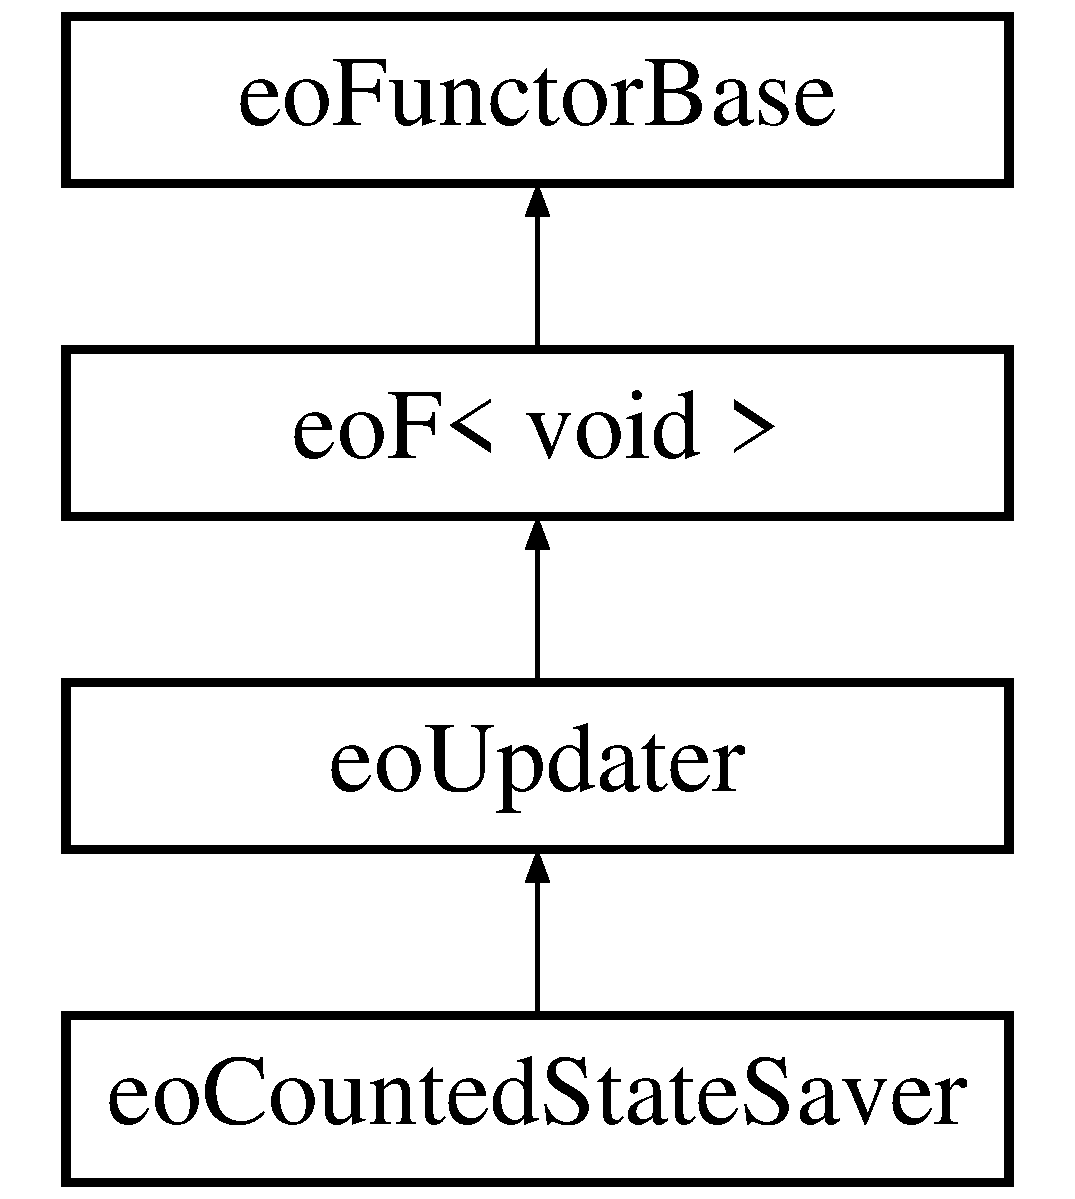
\includegraphics[height=4cm]{classeo_counted_state_saver}
\end{center}
\end{figure}
\subsection*{Public Member Functions}
\begin{CompactItemize}
\item 
{\bf eo\-Counted\-State\-Saver} (unsigned \_\-interval, const {\bf eo\-State} \&\_\-state, std::string \_\-prefix, bool \_\-save\-On\-Last\-Call, std::string \_\-extension=\char`\"{}sav\char`\"{}, unsigned \_\-counter=0)\label{classeo_counted_state_saver_a0}

\item 
{\bf eo\-Counted\-State\-Saver} (unsigned \_\-interval, const {\bf eo\-State} \&\_\-state, std::string \_\-prefix=\char`\"{}state\char`\"{}, std::string \_\-extension=\char`\"{}sav\char`\"{}, unsigned \_\-counter=0)\label{classeo_counted_state_saver_a1}

\item 
virtual void {\bf last\-Call} (void)\label{classeo_counted_state_saver_a2}

\item 
void {\bf operator()} (void)\label{classeo_counted_state_saver_a3}

\begin{CompactList}\small\item\em The pure virtual function that needs to be implemented by the subclass. \item\end{CompactList}\item 
virtual std::string {\bf class\-Name} (void) const \label{classeo_counted_state_saver_a4}

\end{CompactItemize}
\subsection*{Private Member Functions}
\begin{CompactItemize}
\item 
void {\bf do\-It\-Now} (void)\label{classeo_counted_state_saver_d0}

\end{CompactItemize}
\subsection*{Private Attributes}
\begin{CompactItemize}
\item 
const {\bf eo\-State} \& {\bf state}\label{classeo_counted_state_saver_r0}

\item 
const unsigned {\bf interval}\label{classeo_counted_state_saver_r1}

\item 
unsigned {\bf counter}\label{classeo_counted_state_saver_r2}

\item 
bool {\bf save\-On\-Last\-Call}\label{classeo_counted_state_saver_r3}

\item 
const std::string {\bf prefix}\label{classeo_counted_state_saver_r4}

\item 
const std::string {\bf extension}\label{classeo_counted_state_saver_r5}

\end{CompactItemize}


\subsection{Detailed Description}
an {\bf eo\-Updater}{\rm (p.\,\pageref{classeo_updater})} that saves a state every given generations 



Definition at line 127 of file eo\-Updater.h.

The documentation for this class was generated from the following files:\begin{CompactItemize}
\item 
eo\-Updater.h\item 
eo\-Updater.cpp\end{CompactItemize}

\section{Cov Class Reference}
\label{class_cov}\index{Cov@{Cov}}
Single covariance between two variates.  


{\tt \#include $<$stats.h$>$}

\subsection*{Public Member Functions}
\begin{CompactItemize}
\item 
void {\bf update} (double a, double b)\label{class_cov_a1}

\item 
double {\bf get\_\-meana} () const \label{class_cov_a2}

\item 
double {\bf get\_\-meanb} () const \label{class_cov_a3}

\item 
double {\bf get\_\-cov} () const \label{class_cov_a4}

\end{CompactItemize}
\subsection*{Private Attributes}
\begin{CompactItemize}
\item 
double {\bf n}\label{class_cov_r0}

\item 
double {\bf meana}\label{class_cov_r1}

\item 
double {\bf meanb}\label{class_cov_r2}

\item 
double {\bf sumcov}\label{class_cov_r3}

\end{CompactItemize}


\subsection{Detailed Description}
Single covariance between two variates. 



Definition at line 58 of file stats.h.

The documentation for this class was generated from the following file:\begin{CompactItemize}
\item 
stats.h\end{CompactItemize}

\section{eo\-Ctrl\-CContinue$<$ EOT $>$ Class Template Reference}
\label{classeo_ctrl_c_continue}\index{eoCtrlCContinue@{eoCtrlCContinue}}
Ctrl C handling: this {\bf eo\-Continue}{\rm (p.\,\pageref{classeo_continue})} tells whether the user pressed Ctrl C.  


{\tt \#include $<$eo\-Ctrl\-CContinue.h$>$}

Inheritance diagram for eo\-Ctrl\-CContinue$<$ EOT $>$::\begin{figure}[H]
\begin{center}
\leavevmode
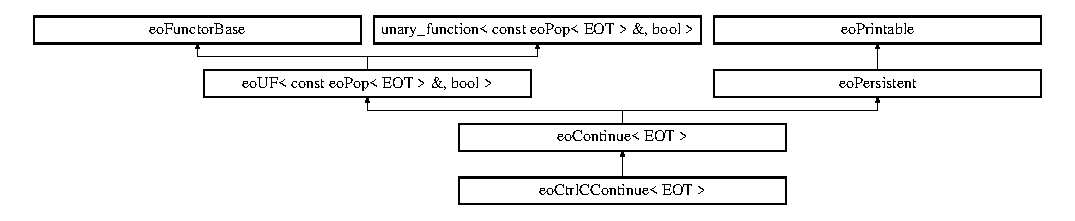
\includegraphics[height=2.52252cm]{classeo_ctrl_c_continue}
\end{center}
\end{figure}
\subsection*{Public Member Functions}
\begin{CompactItemize}
\item 
{\bf eo\-Ctrl\-CContinue} ()\label{classeo_ctrl_c_continue_a0}

\begin{CompactList}\small\item\em Ctor : installs the signal handler. \item\end{CompactList}\item 
virtual bool {\bf operator()} (const {\bf eo\-Pop}$<$ {\bf EOT} $>$ \&\_\-v\-EO)\label{classeo_ctrl_c_continue_a1}

\begin{CompactList}\small\item\em Returns false when Ctrl C has been typed in reached. \item\end{CompactList}\item 
virtual std::string {\bf class\-Name} (void) const \label{classeo_ctrl_c_continue_a2}

\end{CompactItemize}


\subsection{Detailed Description}
\subsubsection*{template$<$class EOT$>$ class eo\-Ctrl\-CContinue$<$ EOT $>$}

Ctrl C handling: this {\bf eo\-Continue}{\rm (p.\,\pageref{classeo_continue})} tells whether the user pressed Ctrl C. 



Definition at line 45 of file eo\-Ctrl\-CContinue.h.

The documentation for this class was generated from the following file:\begin{CompactItemize}
\item 
eo\-Ctrl\-CContinue.h\end{CompactItemize}

\section{eo\-Det\-Bit\-Flip$<$ Chrom $>$ Class Template Reference}
\label{classeo_det_bit_flip}\index{eoDetBitFlip@{eoDetBitFlip}}
eo\-Det\-Bit\-Flip --$>$ changes exactly k bits  


{\tt \#include $<$ga/eo\-Bit\-Op.h$>$}

Inheritance diagram for eo\-Det\-Bit\-Flip$<$ Chrom $>$::\begin{figure}[H]
\begin{center}
\leavevmode
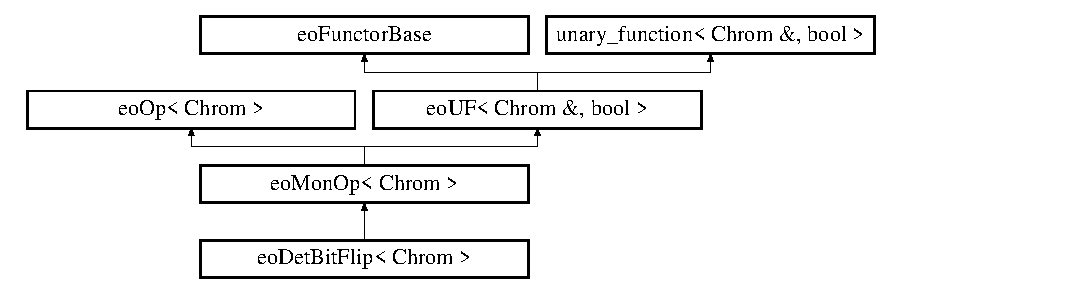
\includegraphics[height=3.50548cm]{classeo_det_bit_flip}
\end{center}
\end{figure}
\subsection*{Public Member Functions}
\begin{CompactItemize}
\item 
{\bf eo\-Det\-Bit\-Flip} (const unsigned \&\_\-num\_\-bit=1)
\begin{CompactList}\small\item\em (Default) Constructor. \item\end{CompactList}\item 
virtual std::string {\bf class\-Name} () const \label{classeo_det_bit_flip_a1}

\begin{CompactList}\small\item\em The class name. \item\end{CompactList}\item 
bool {\bf operator()} (Chrom \&chrom)
\begin{CompactList}\small\item\em Change num\_\-bit bits. \item\end{CompactList}\end{CompactItemize}
\subsection*{Private Attributes}
\begin{CompactItemize}
\item 
unsigned {\bf num\_\-bit}\label{classeo_det_bit_flip_r0}

\end{CompactItemize}


\subsection{Detailed Description}
\subsubsection*{template$<$class Chrom$>$ class eo\-Det\-Bit\-Flip$<$ Chrom $>$}

eo\-Det\-Bit\-Flip --$>$ changes exactly k bits 



Definition at line 67 of file eo\-Bit\-Op.h.

\subsection{Constructor \& Destructor Documentation}
\index{eoDetBitFlip@{eo\-Det\-Bit\-Flip}!eoDetBitFlip@{eoDetBitFlip}}
\index{eoDetBitFlip@{eoDetBitFlip}!eoDetBitFlip@{eo\-Det\-Bit\-Flip}}
\subsubsection{\setlength{\rightskip}{0pt plus 5cm}template$<$class Chrom$>$ {\bf eo\-Det\-Bit\-Flip}$<$ Chrom $>$::{\bf eo\-Det\-Bit\-Flip} (const unsigned \& {\em \_\-num\_\-bit} = {\tt 1})\hspace{0.3cm}{\tt  [inline]}}\label{classeo_det_bit_flip_a0}


(Default) Constructor. 

\begin{Desc}
\item[Parameters:]
\begin{description}
\item[{\em \_\-num\_\-bit}]The number of bits to change default is one - equivalent to eo\-One\-Bit\-Flip then \end{description}
\end{Desc}


Definition at line 75 of file eo\-Bit\-Op.h.

\subsection{Member Function Documentation}
\index{eoDetBitFlip@{eo\-Det\-Bit\-Flip}!operator()@{operator()}}
\index{operator()@{operator()}!eoDetBitFlip@{eo\-Det\-Bit\-Flip}}
\subsubsection{\setlength{\rightskip}{0pt plus 5cm}template$<$class Chrom$>$ bool {\bf eo\-Det\-Bit\-Flip}$<$ Chrom $>$::operator() (Chrom \& {\em chrom})\hspace{0.3cm}{\tt  [inline, virtual]}}\label{classeo_det_bit_flip_a2}


Change num\_\-bit bits. 

\begin{Desc}
\item[Parameters:]
\begin{description}
\item[{\em chrom}]The cromosome which one bit is going to be changed. \end{description}
\end{Desc}


Implements {\bf eo\-UF$<$ Chrom \&, bool $>$} {\rm (p.\,\pageref{classeo_u_f_a1})}.

Definition at line 84 of file eo\-Bit\-Op.h.

The documentation for this class was generated from the following file:\begin{CompactItemize}
\item 
eo\-Bit\-Op.h\end{CompactItemize}

\section{eo\-Deterministic\-Sa\-DReplacement$<$ EOT $>$ Class Template Reference}
\label{classeo_deterministic_sa_d_replacement}\index{eoDeterministicSaDReplacement@{eoDeterministicSaDReplacement}}
eo\-Deterministic\-Sa\-DReplacement: replacement strategy that is just, in sequence saves best and kill worse from parents + saves best and kill worse from offspring + merge remaining (neither save nor killed) parents and offspring + reduce that merged population = returns reduced pop + best parents + best offspring  


{\tt \#include $<$eo\-Survive\-And\-Die.h$>$}

Inheritance diagram for eo\-Deterministic\-Sa\-DReplacement$<$ EOT $>$::\begin{figure}[H]
\begin{center}
\leavevmode
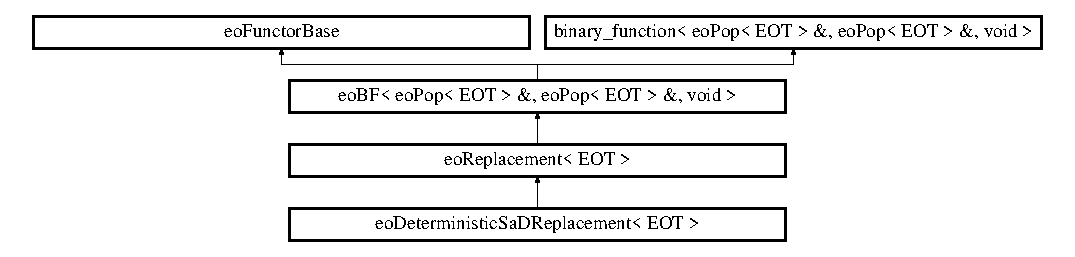
\includegraphics[height=3.01075cm]{classeo_deterministic_sa_d_replacement}
\end{center}
\end{figure}
\subsection*{Public Member Functions}
\begin{CompactItemize}
\item 
{\bf eo\-Deterministic\-Sa\-DReplacement} ({\bf eo\-Reduce}$<$ {\bf EOT} $>$ \&\_\-reduce\-Global, double \_\-survive\-Parents, double \_\-die\-Parents=0, double \_\-survive\-Offspring=0, double \_\-die\-Offspring=0, bool \_\-interpret\_\-as\_\-rate=true)\label{classeo_deterministic_sa_d_replacement_a0}

\begin{CompactList}\small\item\em Constructor with reduce. \item\end{CompactList}\item 
{\bf eo\-Deterministic\-Sa\-DReplacement} (double \_\-survive\-Parents, double \_\-die\-Parents=0, double \_\-survive\-Offspring=0, double \_\-die\-Offspring=0, bool \_\-interpret\_\-as\_\-rate=true)\label{classeo_deterministic_sa_d_replacement_a1}

\begin{CompactList}\small\item\em Constructor with default truncate used as reduce. \item\end{CompactList}\item 
void {\bf operator()} ({\bf eo\-Pop}$<$ {\bf EOT} $>$ \&\_\-parents, {\bf eo\-Pop}$<$ {\bf EOT} $>$ \&\_\-offspring)\label{classeo_deterministic_sa_d_replacement_a2}

\begin{CompactList}\small\item\em The pure virtual function that needs to be implemented by the subclass. \item\end{CompactList}\end{CompactItemize}
\subsection*{Private Attributes}
\begin{CompactItemize}
\item 
{\bf eo\-Reduce}$<$ {\bf EOT} $>$ \& {\bf reduce\-Global}\label{classeo_deterministic_sa_d_replacement_r0}

\item 
{\bf eo\-Deterministic\-Survive\-And\-Die}$<$ {\bf EOT} $>$ {\bf s\-Ad\-Parents}\label{classeo_deterministic_sa_d_replacement_r1}

\item 
{\bf eo\-Deterministic\-Survive\-And\-Die}$<$ {\bf EOT} $>$ {\bf s\-Ad\-Offspring}\label{classeo_deterministic_sa_d_replacement_r2}

\item 
{\bf eo\-Plus}$<$ {\bf EOT} $>$ {\bf plus}\label{classeo_deterministic_sa_d_replacement_r3}

\item 
{\bf eo\-Truncate}$<$ {\bf EOT} $>$ {\bf truncate}\label{classeo_deterministic_sa_d_replacement_r4}

\end{CompactItemize}


\subsection{Detailed Description}
\subsubsection*{template$<$class EOT$>$ class eo\-Deterministic\-Sa\-DReplacement$<$ EOT $>$}

eo\-Deterministic\-Sa\-DReplacement: replacement strategy that is just, in sequence saves best and kill worse from parents + saves best and kill worse from offspring + merge remaining (neither save nor killed) parents and offspring + reduce that merged population = returns reduced pop + best parents + best offspring 

An obvious use is as strong elitist strategy, i.e. preserving best parents, and reducing (either offspring or parents+offspring) 



Definition at line 132 of file eo\-Survive\-And\-Die.h.

The documentation for this class was generated from the following file:\begin{CompactItemize}
\item 
eo\-Survive\-And\-Die.h\end{CompactItemize}

\section{eo\-Deterministic\-Survive\-And\-Die$<$ EOT $>$ Class Template Reference}
\label{classeo_deterministic_survive_and_die}\index{eoDeterministicSurviveAndDie@{eoDeterministicSurviveAndDie}}
An instance (theonly one as of today, Dec.  


{\tt \#include $<$eo\-Survive\-And\-Die.h$>$}

Inheritance diagram for eo\-Deterministic\-Survive\-And\-Die$<$ EOT $>$::\begin{figure}[H]
\begin{center}
\leavevmode
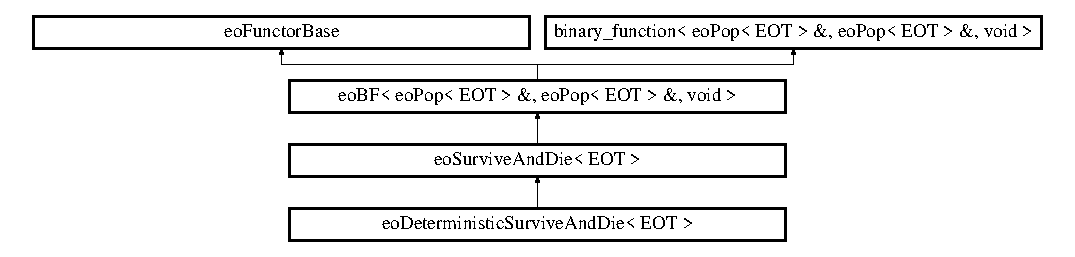
\includegraphics[height=3.01075cm]{classeo_deterministic_survive_and_die}
\end{center}
\end{figure}
\subsection*{Public Member Functions}
\begin{CompactItemize}
\item 
{\bf eo\-Deterministic\-Survive\-And\-Die} (double \_\-survive, double \_\-die, bool \_\-interpret\_\-as\_\-rate=true)\label{classeo_deterministic_survive_and_die_a0}

\begin{CompactList}\small\item\em constructor \item\end{CompactList}\item 
void {\bf operator()} ({\bf eo\-Pop}$<$ {\bf EOT} $>$ \&\_\-pop, {\bf eo\-Pop}$<$ {\bf EOT} $>$ \&\_\-lucky\-Guys)\label{classeo_deterministic_survive_and_die_a1}

\begin{CompactList}\small\item\em The pure virtual function that needs to be implemented by the subclass. \item\end{CompactList}\end{CompactItemize}


\subsection{Detailed Description}
\subsubsection*{template$<$class EOT$>$ class eo\-Deterministic\-Survive\-And\-Die$<$ EOT $>$}

An instance (theonly one as of today, Dec. 

20, 2000) of an {\bf eo\-Survive\-And\-Die}{\rm (p.\,\pageref{classeo_survive_and_die})}, that does everything deterministically

Used in {\bf eo\-Deterministic\-Sa\-DReplacement}{\rm (p.\,\pageref{classeo_deterministic_sa_d_replacement})}. 



Definition at line 73 of file eo\-Survive\-And\-Die.h.

The documentation for this class was generated from the following file:\begin{CompactItemize}
\item 
eo\-Survive\-And\-Die.h\end{CompactItemize}

\section{eo\-Det\-Select$<$ EOT $>$ Class Template Reference}
\label{classeo_det_select}\index{eoDetSelect@{eoDetSelect}}
eo\-Det\-Select selects many individuals determinisctically  


{\tt \#include $<$eo\-Det\-Select.h$>$}

Inheritance diagram for eo\-Det\-Select$<$ EOT $>$::\begin{figure}[H]
\begin{center}
\leavevmode
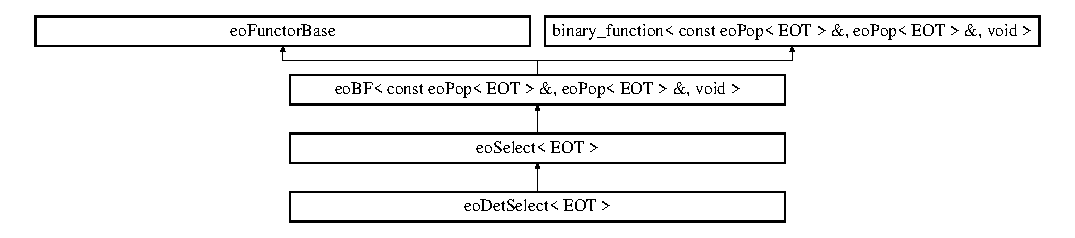
\includegraphics[height=2.75184cm]{classeo_det_select}
\end{center}
\end{figure}
\subsection*{Public Member Functions}
\begin{CompactItemize}
\item 
{\bf eo\-Det\-Select} (double \_\-rate=1.0, bool \_\-interpret\_\-as\_\-rate=true)\label{classeo_det_select_a0}

\begin{CompactList}\small\item\em init \item\end{CompactList}\item 
virtual void {\bf operator()} (const {\bf eo\-Pop}$<$ {\bf EOT} $>$ \&\_\-source, {\bf eo\-Pop}$<$ {\bf EOT} $>$ \&\_\-dest)
\end{CompactItemize}
\subsection*{Private Attributes}
\begin{CompactItemize}
\item 
{\bf eo\-How\-Many} {\bf how\-Many}\label{classeo_det_select_r0}

\end{CompactItemize}


\subsection{Detailed Description}
\subsubsection*{template$<$class EOT$>$ class eo\-Det\-Select$<$ EOT $>$}

eo\-Det\-Select selects many individuals determinisctically 



Definition at line 40 of file eo\-Det\-Select.h.

\subsection{Member Function Documentation}
\index{eoDetSelect@{eo\-Det\-Select}!operator()@{operator()}}
\index{operator()@{operator()}!eoDetSelect@{eo\-Det\-Select}}
\subsubsection{\setlength{\rightskip}{0pt plus 5cm}template$<$class EOT$>$ virtual void {\bf eo\-Det\-Select}$<$ {\bf EOT} $>$::operator() (const {\bf eo\-Pop}$<$ {\bf EOT} $>$ \& {\em \_\-source}, {\bf eo\-Pop}$<$ {\bf EOT} $>$ \& {\em \_\-dest})\hspace{0.3cm}{\tt  [inline, virtual]}}\label{classeo_det_select_a1}


\begin{Desc}
\item[Parameters:]
\begin{description}
\item[{\em \_\-source}]the source population \item[{\em \_\-dest}]the resulting population (size of this population is given by the How\-Many data It empties the destination and adds the selection into it) \end{description}
\end{Desc}


Implements {\bf eo\-BF$<$ const eo\-Pop$<$ EOT $>$ \&, eo\-Pop$<$ EOT $>$ \&, void $>$} {\rm (p.\,\pageref{classeo_b_f_a1})}.

Definition at line 53 of file eo\-Det\-Select.h.

The documentation for this class was generated from the following file:\begin{CompactItemize}
\item 
eo\-Det\-Select.h\end{CompactItemize}

\section{eo\-Det\-Tournament\-Select$<$ EOT $>$ Class Template Reference}
\label{classeo_det_tournament_select}\index{eoDetTournamentSelect@{eoDetTournamentSelect}}
eo\-Det\-Tournament\-Select: a selection method that selects ONE individual by deterministic tournament -MS- 24/10/99  


{\tt \#include $<$eo\-Det\-Tournament\-Select.h$>$}

Inheritance diagram for eo\-Det\-Tournament\-Select$<$ EOT $>$::\begin{figure}[H]
\begin{center}
\leavevmode
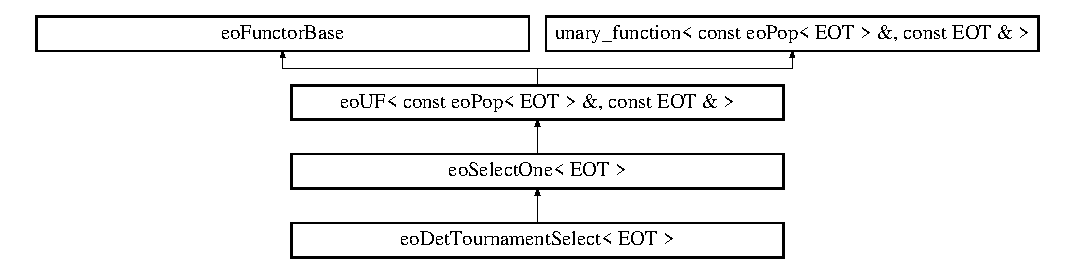
\includegraphics[height=3.23699cm]{classeo_det_tournament_select}
\end{center}
\end{figure}
\subsection*{Public Member Functions}
\begin{CompactItemize}
\item 
{\bf eo\-Det\-Tournament\-Select} (unsigned \_\-t\-Size=2)\label{classeo_det_tournament_select_a0}

\item 
virtual const {\bf EOT} \& {\bf operator()} (const {\bf eo\-Pop}$<$ {\bf EOT} $>$ \&\_\-pop)\label{classeo_det_tournament_select_a1}

\begin{CompactList}\small\item\em The pure virtual function that needs to be implemented by the subclass. \item\end{CompactList}\end{CompactItemize}
\subsection*{Private Attributes}
\begin{CompactItemize}
\item 
unsigned {\bf t\-Size}\label{classeo_det_tournament_select_r0}

\end{CompactItemize}


\subsection{Detailed Description}
\subsubsection*{template$<$class EOT$>$ class eo\-Det\-Tournament\-Select$<$ EOT $>$}

eo\-Det\-Tournament\-Select: a selection method that selects ONE individual by deterministic tournament -MS- 24/10/99 



Definition at line 44 of file eo\-Det\-Tournament\-Select.h.

The documentation for this class was generated from the following file:\begin{CompactItemize}
\item 
eo\-Det\-Tournament\-Select.h\end{CompactItemize}

\section{eo\-Det\-Tournament\-Truncate$<$ EOT $>$ Class Template Reference}
\label{classeo_det_tournament_truncate}\index{eoDetTournamentTruncate@{eoDetTournamentTruncate}}
a truncate class based on a repeated deterministic (reverse!) tournament To be used in SSGA-like replacements (e.g.  


{\tt \#include $<$eo\-Reduce.h$>$}

Inheritance diagram for eo\-Det\-Tournament\-Truncate$<$ EOT $>$::\begin{figure}[H]
\begin{center}
\leavevmode
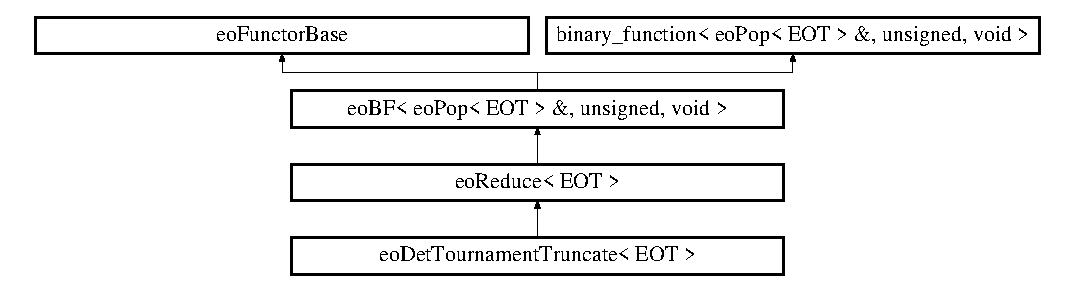
\includegraphics[height=3.45679cm]{classeo_det_tournament_truncate}
\end{center}
\end{figure}
\subsection*{Public Member Functions}
\begin{CompactItemize}
\item 
{\bf eo\-Det\-Tournament\-Truncate} (unsigned \_\-t\_\-size)\label{classeo_det_tournament_truncate_a0}

\item 
void {\bf operator()} ({\bf eo\-Pop}$<$ {\bf EOT} $>$ \&\_\-newgen, unsigned \_\-newsize)\label{classeo_det_tournament_truncate_a1}

\begin{CompactList}\small\item\em The pure virtual function that needs to be implemented by the subclass. \item\end{CompactList}\end{CompactItemize}
\subsection*{Private Attributes}
\begin{CompactItemize}
\item 
unsigned {\bf t\_\-size}\label{classeo_det_tournament_truncate_r0}

\end{CompactItemize}


\subsection{Detailed Description}
\subsubsection*{template$<$class EOT$>$ class eo\-Det\-Tournament\-Truncate$<$ EOT $>$}

a truncate class based on a repeated deterministic (reverse!) tournament To be used in SSGA-like replacements (e.g. 

see {\bf eo\-SSGADet\-Tournament\-Replacement}{\rm (p.\,\pageref{classeo_s_s_g_a_det_tournament_replacement})}) 



Definition at line 188 of file eo\-Reduce.h.

The documentation for this class was generated from the following file:\begin{CompactItemize}
\item 
eo\-Reduce.h\end{CompactItemize}

\section{eo\-Det\-Tournament\-Truncate\-Split$<$ EOT $>$ Class Template Reference}
\label{classeo_det_tournament_truncate_split}\index{eoDetTournamentTruncateSplit@{eoDetTournamentTruncateSplit}}
a Reduce\-Split class based on a repeated deterministic (reverse!) tournament To be used in SSGA-like replacements (e.g.  


{\tt \#include $<$eo\-Reduce\-Split.h$>$}

Inheritance diagram for eo\-Det\-Tournament\-Truncate\-Split$<$ EOT $>$::\begin{figure}[H]
\begin{center}
\leavevmode
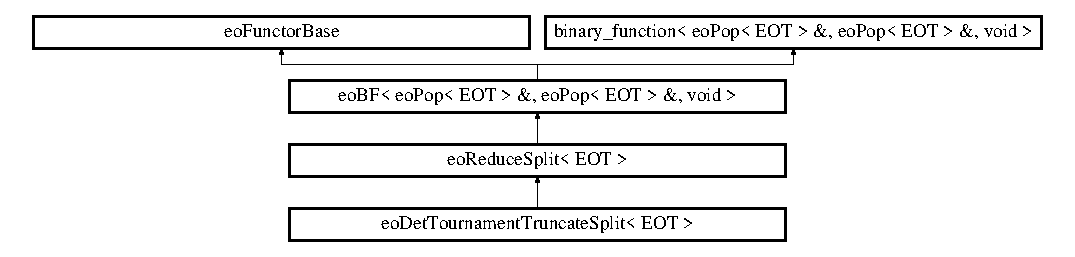
\includegraphics[height=3.01075cm]{classeo_det_tournament_truncate_split}
\end{center}
\end{figure}
\subsection*{Public Member Functions}
\begin{CompactItemize}
\item 
{\bf eo\-Det\-Tournament\-Truncate\-Split} (unsigned \_\-t\_\-size, {\bf eo\-How\-Many} \_\-how\-Many, bool \_\-return\-Eliminated=false)\label{classeo_det_tournament_truncate_split_a0}

\begin{CompactList}\small\item\em Ctor: must provide amount of reduction, and whether or not you need to return the eliminated guys. \item\end{CompactList}\item 
void {\bf operator()} ({\bf eo\-Pop}$<$ {\bf EOT} $>$ \&\_\-newgen, {\bf eo\-Pop}$<$ {\bf EOT} $>$ \&\_\-eliminated)\label{classeo_det_tournament_truncate_split_a1}

\begin{CompactList}\small\item\em Performs repeated inverse\_\-deterministic\_\-tournament on the pop. \item\end{CompactList}\end{CompactItemize}
\subsection*{Private Attributes}
\begin{CompactItemize}
\item 
unsigned {\bf t\_\-size}\label{classeo_det_tournament_truncate_split_r0}

\item 
{\bf eo\-How\-Many} {\bf how\-Many}\label{classeo_det_tournament_truncate_split_r1}

\item 
bool {\bf return\-Eliminated}\label{classeo_det_tournament_truncate_split_r2}

\end{CompactItemize}


\subsection{Detailed Description}
\subsubsection*{template$<$class EOT$>$ class eo\-Det\-Tournament\-Truncate\-Split$<$ EOT $>$}

a Reduce\-Split class based on a repeated deterministic (reverse!) tournament To be used in SSGA-like replacements (e.g. 

see {\bf eo\-SSGADet\-Tournament\-Replacement}{\rm (p.\,\pageref{classeo_s_s_g_a_det_tournament_replacement})}) 



Definition at line 205 of file eo\-Reduce\-Split.h.

The documentation for this class was generated from the following file:\begin{CompactItemize}
\item 
eo\-Reduce\-Split.h\end{CompactItemize}

\section{eo\-Det\-Tournament\-Worth\-Select$<$ EOT, Worth\-T $>$ Class Template Reference}
\label{classeo_det_tournament_worth_select}\index{eoDetTournamentWorthSelect@{eoDetTournamentWorthSelect}}
An instance of eo\-Select\-Perf2Worth that does selection from the Worthes using a ...  


{\tt \#include $<$eo\-Select\-From\-Worth.h$>$}

Inheritance diagram for eo\-Det\-Tournament\-Worth\-Select$<$ EOT, Worth\-T $>$::\begin{figure}[H]
\begin{center}
\leavevmode
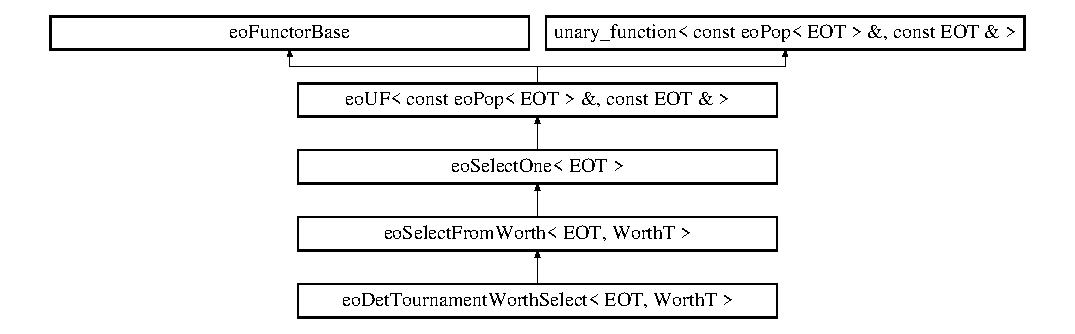
\includegraphics[height=4.04624cm]{classeo_det_tournament_worth_select}
\end{center}
\end{figure}
\subsection*{Public Types}
\begin{CompactItemize}
\item 
typedef std::vector$<$ Worth\-T $>$::iterator {\bf worth\-Iterator}\label{classeo_det_tournament_worth_select_w0}

\end{CompactItemize}
\subsection*{Public Member Functions}
\begin{CompactItemize}
\item 
{\bf eo\-Det\-Tournament\-Worth\-Select} ({\bf eo\-Perf2Worth}$<$ {\bf EOT}, Worth\-T $>$ \&perf2Worth, unsigned \_\-t\-Size)\label{classeo_det_tournament_worth_select_a0}

\item 
virtual const {\bf EOT} \& {\bf operator()} (const {\bf eo\-Pop}$<$ {\bf EOT} $>$ \&pop)\label{classeo_det_tournament_worth_select_a1}

\begin{CompactList}\small\item\em The pure virtual function that needs to be implemented by the subclass. \item\end{CompactList}\end{CompactItemize}
\subsection*{Private Attributes}
\begin{CompactItemize}
\item 
unsigned {\bf t\-Size}\label{classeo_det_tournament_worth_select_r0}

\end{CompactItemize}


\subsection{Detailed Description}
\subsubsection*{template$<$class EOT, class Worth\-T = double$>$ class eo\-Det\-Tournament\-Worth\-Select$<$ EOT, Worth\-T $>$}

An instance of eo\-Select\-Perf2Worth that does selection from the Worthes using a ... 

determinisitic tournament, yes! 



Definition at line 91 of file eo\-Select\-From\-Worth.h.

The documentation for this class was generated from the following file:\begin{CompactItemize}
\item 
eo\-Select\-From\-Worth.h\end{CompactItemize}

\section{eo\-Det\-Uniform\-Mutation$<$ EOT $>$ Class Template Reference}
\label{classeo_det_uniform_mutation}\index{eoDetUniformMutation@{eoDetUniformMutation}}
eo\-Det\-Uniform\-Mutation --$>$ changes exactly k values of the std::vector by uniform choice with range epsilon  


{\tt \#include $<$Tutorial/eo\-Real\-Op.h$>$}

Inheritance diagram for eo\-Det\-Uniform\-Mutation$<$ EOT $>$::\begin{figure}[H]
\begin{center}
\leavevmode
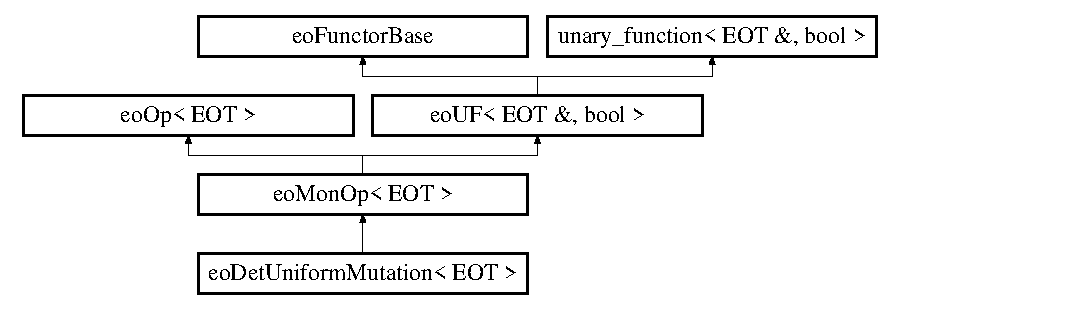
\includegraphics[height=3.71476cm]{classeo_det_uniform_mutation}
\end{center}
\end{figure}
\subsection*{Public Member Functions}
\begin{CompactItemize}
\item 
{\bf eo\-Det\-Uniform\-Mutation} (const double \&\_\-epsilon, const unsigned \&\_\-no=1)
\begin{CompactList}\small\item\em (Default) Constructor for homogeneous genotype it's there mostly for backward compatibility \item\end{CompactList}\item 
{\bf eo\-Det\-Uniform\-Mutation} ({\bf eo\-Real\-Vector\-Bounds} \&\_\-bounds, const double \&\_\-epsilon, const unsigned \&\_\-no=1)
\begin{CompactList}\small\item\em Constructor with bounds. \item\end{CompactList}\item 
{\bf eo\-Det\-Uniform\-Mutation} ({\bf eo\-Real\-Vector\-Bounds} \&\_\-bounds, const std::vector$<$ double $>$ \&\_\-epsilon, const unsigned \&\_\-no=1)
\begin{CompactList}\small\item\em Constructor with bounds and full std::vector of epsilon. \item\end{CompactList}\item 
virtual std::string {\bf class\-Name} () const \label{classeo_det_uniform_mutation_a3}

\begin{CompactList}\small\item\em The class name. \item\end{CompactList}\item 
bool {\bf operator()} ({\bf EOT} \&\_\-eo)
\begin{CompactList}\small\item\em Do it! \item\end{CompactList}\end{CompactItemize}
\subsection*{Private Attributes}
\begin{CompactItemize}
\item 
bool {\bf homogeneous}\label{classeo_det_uniform_mutation_r0}

\item 
{\bf eo\-Real\-Vector\-Bounds} \& {\bf bounds}\label{classeo_det_uniform_mutation_r1}

\item 
std::vector$<$ double $>$ {\bf epsilon}\label{classeo_det_uniform_mutation_r2}

\item 
unsigned {\bf no}\label{classeo_det_uniform_mutation_r3}

\end{CompactItemize}


\subsection{Detailed Description}
\subsubsection*{template$<$class EOT$>$ class eo\-Det\-Uniform\-Mutation$<$ EOT $>$}

eo\-Det\-Uniform\-Mutation --$>$ changes exactly k values of the std::vector by uniform choice with range epsilon 



Definition at line 144 of file eo\-Real\-Op.h.

\subsection{Constructor \& Destructor Documentation}
\index{eoDetUniformMutation@{eo\-Det\-Uniform\-Mutation}!eoDetUniformMutation@{eoDetUniformMutation}}
\index{eoDetUniformMutation@{eoDetUniformMutation}!eoDetUniformMutation@{eo\-Det\-Uniform\-Mutation}}
\subsubsection{\setlength{\rightskip}{0pt plus 5cm}template$<$class EOT$>$ {\bf eo\-Det\-Uniform\-Mutation}$<$ {\bf EOT} $>$::{\bf eo\-Det\-Uniform\-Mutation} (const double \& {\em \_\-epsilon}, const unsigned \& {\em \_\-no} = {\tt 1})\hspace{0.3cm}{\tt  [inline]}}\label{classeo_det_uniform_mutation_a0}


(Default) Constructor for homogeneous genotype it's there mostly for backward compatibility 

\begin{Desc}
\item[Parameters:]
\begin{description}
\item[{\em \_\-epsilon}]the range for uniform nutation \item[{\em number}]of coordinate to modify \end{description}
\end{Desc}


Definition at line 154 of file eo\-Real\-Op.h.\index{eoDetUniformMutation@{eo\-Det\-Uniform\-Mutation}!eoDetUniformMutation@{eoDetUniformMutation}}
\index{eoDetUniformMutation@{eoDetUniformMutation}!eoDetUniformMutation@{eo\-Det\-Uniform\-Mutation}}
\subsubsection{\setlength{\rightskip}{0pt plus 5cm}template$<$class EOT$>$ {\bf eo\-Det\-Uniform\-Mutation}$<$ {\bf EOT} $>$::{\bf eo\-Det\-Uniform\-Mutation} ({\bf eo\-Real\-Vector\-Bounds} \& {\em \_\-bounds}, const double \& {\em \_\-epsilon}, const unsigned \& {\em \_\-no} = {\tt 1})\hspace{0.3cm}{\tt  [inline]}}\label{classeo_det_uniform_mutation_a1}


Constructor with bounds. 

\begin{Desc}
\item[Parameters:]
\begin{description}
\item[{\em \_\-bounds}]an {\bf eo\-Real\-Vector\-Bounds}{\rm (p.\,\pageref{classeo_real_vector_bounds})} that contains the bounds \item[{\em \_\-epsilon}]the range for uniform nutation (to be scaled if necessary) \item[{\em number}]of coordinate to modify \end{description}
\end{Desc}


Definition at line 164 of file eo\-Real\-Op.h.

References eo\-Real\-Base\-Vector\-Bounds::is\-Bounded(), and eo\-Real\-Base\-Vector\-Bounds::range().\index{eoDetUniformMutation@{eo\-Det\-Uniform\-Mutation}!eoDetUniformMutation@{eoDetUniformMutation}}
\index{eoDetUniformMutation@{eoDetUniformMutation}!eoDetUniformMutation@{eo\-Det\-Uniform\-Mutation}}
\subsubsection{\setlength{\rightskip}{0pt plus 5cm}template$<$class EOT$>$ {\bf eo\-Det\-Uniform\-Mutation}$<$ {\bf EOT} $>$::{\bf eo\-Det\-Uniform\-Mutation} ({\bf eo\-Real\-Vector\-Bounds} \& {\em \_\-bounds}, const std::vector$<$ double $>$ \& {\em \_\-epsilon}, const unsigned \& {\em \_\-no} = {\tt 1})\hspace{0.3cm}{\tt  [inline]}}\label{classeo_det_uniform_mutation_a2}


Constructor with bounds and full std::vector of epsilon. 

\begin{Desc}
\item[Parameters:]
\begin{description}
\item[{\em \_\-bounds}]an {\bf eo\-Real\-Vector\-Bounds}{\rm (p.\,\pageref{classeo_real_vector_bounds})} that contains the bounds \item[{\em \_\-epsilon}]the VECTOR of ranges for uniform mutation \item[{\em number}]of coordinate to modify \end{description}
\end{Desc}


Definition at line 181 of file eo\-Real\-Op.h.

References eo\-Real\-Base\-Vector\-Bounds::is\-Bounded(), and eo\-Real\-Base\-Vector\-Bounds::range().

\subsection{Member Function Documentation}
\index{eoDetUniformMutation@{eo\-Det\-Uniform\-Mutation}!operator()@{operator()}}
\index{operator()@{operator()}!eoDetUniformMutation@{eo\-Det\-Uniform\-Mutation}}
\subsubsection{\setlength{\rightskip}{0pt plus 5cm}template$<$class EOT$>$ bool {\bf eo\-Det\-Uniform\-Mutation}$<$ {\bf EOT} $>$::operator() ({\bf EOT} \& {\em \_\-eo})\hspace{0.3cm}{\tt  [inline, virtual]}}\label{classeo_det_uniform_mutation_a4}


Do it! 

\begin{Desc}
\item[Parameters:]
\begin{description}
\item[{\em \_\-eo}]The indi undergoing the mutation \end{description}
\end{Desc}


Implements {\bf eo\-UF$<$ EOT \&, bool $>$} {\rm (p.\,\pageref{classeo_u_f_a1})}.

Definition at line 199 of file eo\-Real\-Op.h.

References eo\-Real\-Base\-Vector\-Bounds::is\-Max\-Bounded(), eo\-Real\-Base\-Vector\-Bounds::is\-Min\-Bounded(), eo\-Real\-Base\-Vector\-Bounds::maximum(), eo\-Real\-Base\-Vector\-Bounds::minimum(), eo\-Rng::random(), and eo\-Rng::uniform().

The documentation for this class was generated from the following file:\begin{CompactItemize}
\item 
eo\-Real\-Op.h\end{CompactItemize}

\section{eo\-Distance$<$ EOT $>$ Class Template Reference}
\label{classeo_distance}\index{eoDistance@{eoDistance}}
This is a generic class for distance functors: takes 2 things ane returns a double.  


{\tt \#include $<$eo\-Distance.h$>$}

Inheritance diagram for eo\-Distance$<$ EOT $>$::\begin{figure}[H]
\begin{center}
\leavevmode
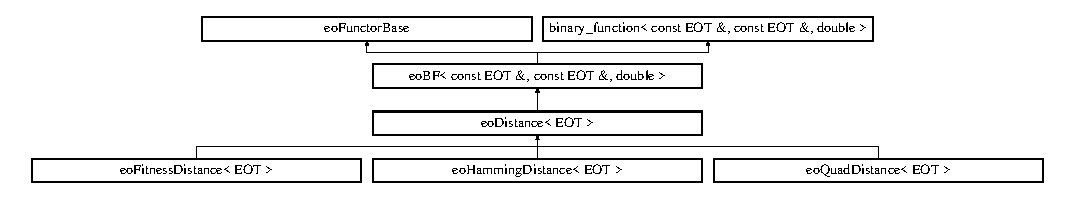
\includegraphics[height=2.22222cm]{classeo_distance}
\end{center}
\end{figure}


\subsection{Detailed Description}
\subsubsection*{template$<$class EOT$>$ class eo\-Distance$<$ EOT $>$}

This is a generic class for distance functors: takes 2 things ane returns a double. 



Definition at line 35 of file eo\-Distance.h.

The documentation for this class was generated from the following file:\begin{CompactItemize}
\item 
eo\-Distance.h\end{CompactItemize}

\section{eo\-Distrib\-Updater$<$ EOT $>$ Class Template Reference}
\label{classeo_distrib_updater}\index{eoDistribUpdater@{eoDistribUpdater}}
Base class for Distribution Evolution Algorithms within {\bf EO}{\rm (p.\,\pageref{class_e_o})}: the update rule of distribution.  


{\tt \#include $<$eo\-Distrib\-Updater.h$>$}

Inheritance diagram for eo\-Distrib\-Updater$<$ EOT $>$::\begin{figure}[H]
\begin{center}
\leavevmode
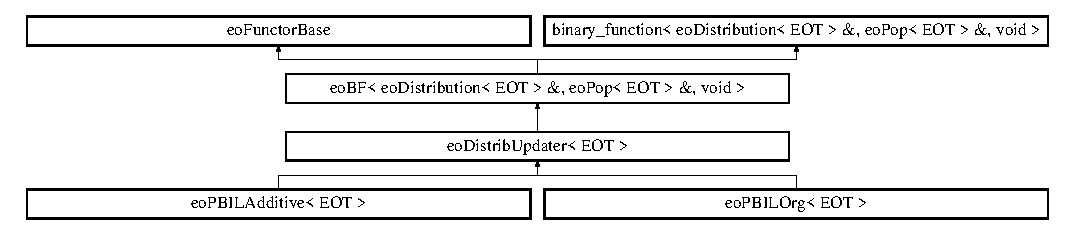
\includegraphics[height=2.71186cm]{classeo_distrib_updater}
\end{center}
\end{figure}
\subsection*{Public Member Functions}
\begin{CompactItemize}
\item 
virtual void {\bf operator()} ({\bf eo\-Distribution}$<$ {\bf EOT} $>$ \&, {\bf eo\-Pop}$<$ {\bf EOT} $>$ \&)=0\label{classeo_distrib_updater_a0}

\begin{CompactList}\small\item\em The pure virtual function that needs to be implemented by the subclass. \item\end{CompactList}\end{CompactItemize}


\subsection{Detailed Description}
\subsubsection*{template$<$class EOT$>$ class eo\-Distrib\-Updater$<$ EOT $>$}

Base class for Distribution Evolution Algorithms within {\bf EO}{\rm (p.\,\pageref{class_e_o})}: the update rule of distribution. 

It takes one distribution and updates it according to one population 



Definition at line 43 of file eo\-Distrib\-Updater.h.

The documentation for this class was generated from the following file:\begin{CompactItemize}
\item 
eo\-Distrib\-Updater.h\end{CompactItemize}

\section{eo\-Distribution$<$ EOT $>$ Class Template Reference}
\label{classeo_distribution}\index{eoDistribution@{eoDistribution}}
Abstract class for Distribution Evolution Algorithms within {\bf EO}{\rm (p.\,\pageref{class_e_o})}: the distribution itself.  


{\tt \#include $<$eo\-Distribution.h$>$}

Inheritance diagram for eo\-Distribution$<$ EOT $>$::\begin{figure}[H]
\begin{center}
\leavevmode
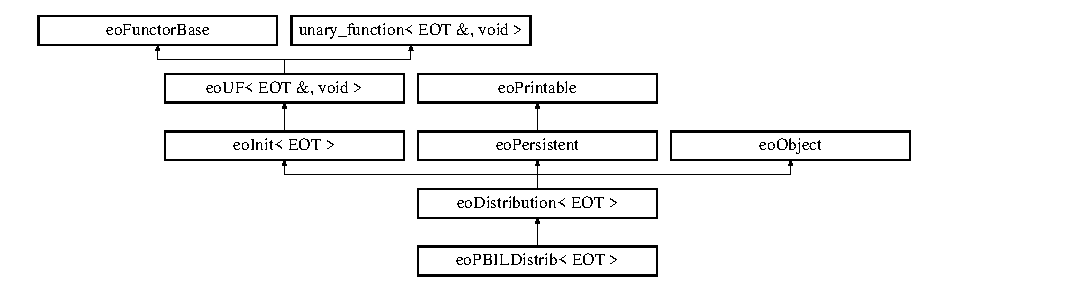
\includegraphics[height=3.48259cm]{classeo_distribution}
\end{center}
\end{figure}
\subsection*{Public Member Functions}
\begin{CompactItemize}
\item 
virtual void {\bf operator()} ({\bf EOT} \&)=0\label{classeo_distribution_a0}

\begin{CompactList}\small\item\em The pure virtual function that needs to be implemented by the subclass. \item\end{CompactList}\end{CompactItemize}


\subsection{Detailed Description}
\subsubsection*{template$<$class EOT$>$ class eo\-Distribution$<$ EOT $>$}

Abstract class for Distribution Evolution Algorithms within {\bf EO}{\rm (p.\,\pageref{class_e_o})}: the distribution itself. 

It basically IS AN {\bf eo\-Init}{\rm (p.\,\pageref{classeo_init})} - {\bf operator()(EOT \&)}{\rm (p.\,\pageref{classeo_distribution_a0})} generates new indis

The instances will probably be {\bf eo\-Value\-Param}{\rm (p.\,\pageref{classeo_value_param})} of some kind see {\bf eo\-PBILDistrib.h}{\rm (p.\,\pageref{eo_p_b_i_l_distrib_8h})} 



Definition at line 45 of file eo\-Distribution.h.

The documentation for this class was generated from the following file:\begin{CompactItemize}
\item 
eo\-Distribution.h\end{CompactItemize}

\section{d\-Matrix Class Reference}
\label{classd_matrix}\index{dMatrix@{dMatrix}}
A helper class for Sharing - to hold distances.  


{\tt \#include $<$eo\-Sharing.h$>$}

\subsection*{Public Member Functions}
\begin{CompactItemize}
\item 
{\bf d\-Matrix} (unsigned \_\-s)\label{classd_matrix_a0}

\item 
double {\bf operator()} (unsigned \_\-i, unsigned \_\-j) const \label{classd_matrix_a1}

\begin{CompactList}\small\item\em simple accessor \item\end{CompactList}\item 
double \& {\bf operator()} (unsigned \_\-i, unsigned \_\-j)\label{classd_matrix_a2}

\begin{CompactList}\small\item\em reference - to set values \item\end{CompactList}\item 
void {\bf print\-On} (std::ostream \&\_\-os)\label{classd_matrix_a3}

\begin{CompactList}\small\item\em just in case \item\end{CompactList}\end{CompactItemize}
\subsection*{Private Attributes}
\begin{CompactItemize}
\item 
unsigned {\bf r\-Size}\label{classd_matrix_r0}

\end{CompactItemize}


\subsection{Detailed Description}
A helper class for Sharing - to hold distances. 



Definition at line 37 of file eo\-Sharing.h.

The documentation for this class was generated from the following file:\begin{CompactItemize}
\item 
eo\-Sharing.h\end{CompactItemize}

\section{eo\-Dominance\-Map$<$ Eo\-Type $>$ Class Template Reference}
\label{classeo_dominance_map}\index{eoDominanceMap@{eoDominanceMap}}
eo\-Dominance\-Map, utility class to calculate and maintain a map (std::vector$<$std::vector$<$bool$>$ $>$) of pareto dominance statistics.  


{\tt \#include $<$eo\-Dominance\-Map.h$>$}

Inheritance diagram for eo\-Dominance\-Map$<$ Eo\-Type $>$::\begin{figure}[H]
\begin{center}
\leavevmode
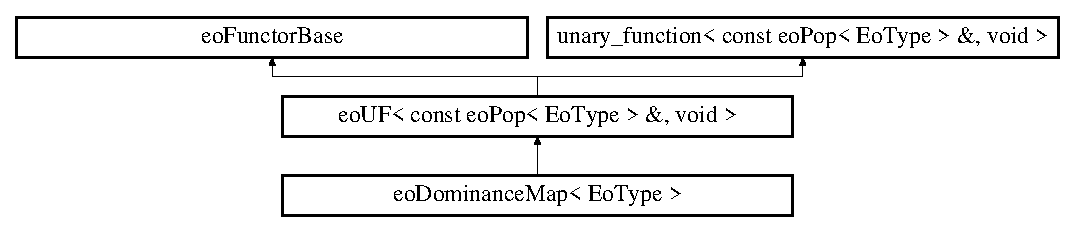
\includegraphics[height=2.67516cm]{classeo_dominance_map}
\end{center}
\end{figure}
\subsection*{Public Member Functions}
\begin{CompactItemize}
\item 
void {\bf clear} ()\label{classeo_dominance_map_a0}

\begin{CompactList}\small\item\em Clears the map. \item\end{CompactList}\item 
void {\bf operator()} (const {\bf eo\-Pop}$<$ {\bf Eo\-Type} $>$ \&\_\-pop)\label{classeo_dominance_map_a1}

\begin{CompactList}\small\item\em Update or create the dominance map. \item\end{CompactList}\item 
void {\bf remove} (unsigned i)\label{classeo_dominance_map_a2}

\begin{CompactList}\small\item\em Removes the domination info for a given individual, thus nothing dominates it and it dominates nothing. \item\end{CompactList}\item 
void {\bf setup} (const {\bf eo\-Pop}$<$ {\bf Eo\-Type} $>$ \&\_\-pop)
\begin{CompactList}\small\item\em Create domination matrix from scratch. \item\end{CompactList}\item 
std::vector$<$ double $>$ {\bf sum\_\-dominators} () const 
\begin{CompactList}\small\item\em For all elements, returns the no. \item\end{CompactList}\item 
std::vector$<$ double $>$ {\bf sum\_\-dominants} () const \label{classeo_dominance_map_a5}

\begin{CompactList}\small\item\em For all elements, returns the number of elements that the element dominates Thus: higher is better It returns a std::vector$<$double$>$ cuz that makes subsequent manipulation that much easier. \item\end{CompactList}\end{CompactItemize}
\subsection*{Private Attributes}
\begin{CompactItemize}
\item 
std::vector$<$ typename Eo\-Type::Fitness $>$ {\bf fitness}\label{classeo_dominance_map_r0}

\end{CompactItemize}


\subsection{Detailed Description}
\subsubsection*{template$<$class Eo\-Type$>$ class eo\-Dominance\-Map$<$ Eo\-Type $>$}

eo\-Dominance\-Map, utility class to calculate and maintain a map (std::vector$<$std::vector$<$bool$>$ $>$) of pareto dominance statistics. 

It is set up such that

if map[i][j] == true then i dominates j

The dominance map can be used to perform pareto ranking ({\bf eo\-Pareto\-Ranking}{\rm (p.\,\pageref{classeo_pareto_ranking})}) or non dominated sorting. For the latter, the {\bf remove()}{\rm (p.\,\pageref{classeo_dominance_map_a2})} member function might come in handy.

\begin{Desc}
\item[{\bf Todo}]make it an {\bf eo\-Stat}{\rm (p.\,\pageref{classeo_stat})}? \end{Desc}




Definition at line 47 of file eo\-Dominance\-Map.h.

\subsection{Member Function Documentation}
\index{eoDominanceMap@{eo\-Dominance\-Map}!setup@{setup}}
\index{setup@{setup}!eoDominanceMap@{eo\-Dominance\-Map}}
\subsubsection{\setlength{\rightskip}{0pt plus 5cm}template$<$class Eo\-Type$>$ void {\bf eo\-Dominance\-Map}$<$ {\bf Eo\-Type} $>$::setup (const {\bf eo\-Pop}$<$ {\bf Eo\-Type} $>$ \& {\em \_\-pop})\hspace{0.3cm}{\tt  [inline]}}\label{classeo_dominance_map_a3}


Create domination matrix from scratch. 

Complexity O(N$^\wedge$2) 

Definition at line 81 of file eo\-Dominance\-Map.h.

Referenced by eo\-Dominance\-Map$<$ EOT $>$::operator()().\index{eoDominanceMap@{eo\-Dominance\-Map}!sum_dominators@{sum\_\-dominators}}
\index{sum_dominators@{sum\_\-dominators}!eoDominanceMap@{eo\-Dominance\-Map}}
\subsubsection{\setlength{\rightskip}{0pt plus 5cm}template$<$class Eo\-Type$>$ std::vector$<$double$>$ {\bf eo\-Dominance\-Map}$<$ {\bf Eo\-Type} $>$::sum\_\-dominators () const\hspace{0.3cm}{\tt  [inline]}}\label{classeo_dominance_map_a4}


For all elements, returns the no. 

of elements that dominate the element Thus: lower is better (and 0 is the front). It returns a std::vector$<$double$>$ cuz that makes subsequent manipulation that much easier 

Definition at line 118 of file eo\-Dominance\-Map.h.

Referenced by eo\-Pareto\-Ranking$<$ EOT $>$::calculate\_\-worths().

The documentation for this class was generated from the following file:\begin{CompactItemize}
\item 
eo\-Dominance\-Map.h\end{CompactItemize}

\section{eo\-Double\-Exchange Class Reference}
\label{classeo_double_exchange}\index{eoDoubleExchange@{eoDoubleExchange}}
Discrete crossover == exchange of values.  


{\tt \#include $<$eo\-Real\-Atom\-Xover.h$>$}

Inheritance diagram for eo\-Double\-Exchange::\begin{figure}[H]
\begin{center}
\leavevmode
\includegraphics[height=2.38552cm]{classeo_double_exchange}
\end{center}
\end{figure}
\subsection*{Public Member Functions}
\begin{CompactItemize}
\item 
{\bf eo\-Double\-Exchange} ()\label{classeo_double_exchange_a0}

\begin{CompactList}\small\item\em (Default) Constructor. \item\end{CompactList}\item 
virtual std::string {\bf class\-Name} () const \label{classeo_double_exchange_a1}

\begin{CompactList}\small\item\em The class name. Used to display statistics. \item\end{CompactList}\item 
bool {\bf operator()} (double \&r1, const double \&r2)\label{classeo_double_exchange_a2}

\begin{CompactList}\small\item\em Exchanges or not the values. \item\end{CompactList}\end{CompactItemize}


\subsection{Detailed Description}
Discrete crossover == exchange of values. 



Definition at line 41 of file eo\-Real\-Atom\-Xover.h.

The documentation for this class was generated from the following file:\begin{CompactItemize}
\item 
eo\-Real\-Atom\-Xover.h\end{CompactItemize}

\section{eo\-Double\-Intermediate Class Reference}
\label{classeo_double_intermediate}\index{eoDoubleIntermediate@{eoDoubleIntermediate}}
Intermediate crossover == linear combination.  


{\tt \#include $<$eo\-Real\-Atom\-Xover.h$>$}

Inheritance diagram for eo\-Double\-Intermediate::\begin{figure}[H]
\begin{center}
\leavevmode
\includegraphics[height=2.38552cm]{classeo_double_intermediate}
\end{center}
\end{figure}
\subsection*{Public Member Functions}
\begin{CompactItemize}
\item 
{\bf eo\-Double\-Intermediate} ()\label{classeo_double_intermediate_a0}

\begin{CompactList}\small\item\em (Default) Constructor. \item\end{CompactList}\item 
virtual std::string {\bf class\-Name} () const \label{classeo_double_intermediate_a1}

\begin{CompactList}\small\item\em The class name. Used to display statistics. \item\end{CompactList}\item 
bool {\bf operator()} (double \&r1, const double \&r2)\label{classeo_double_intermediate_a2}

\begin{CompactList}\small\item\em Linear combination of both parents. \item\end{CompactList}\end{CompactItemize}


\subsection{Detailed Description}
Intermediate crossover == linear combination. 



Definition at line 71 of file eo\-Real\-Atom\-Xover.h.

The documentation for this class was generated from the following file:\begin{CompactItemize}
\item 
eo\-Real\-Atom\-Xover.h\end{CompactItemize}

\section{eo\-Drawable$<$ Object $>$ Class Template Reference}
\label{classeo_drawable}\index{eoDrawable@{eoDrawable}}
eo\-Drawable is a template class that adds a drawing interface to an object.$\backslash$ Requisites for template instantiation are that the object must admit a default ctor and a copy ctor.  


{\tt \#include $<$eo\-Drawable.h$>$}

\subsection*{Public Member Functions}
\begin{CompactItemize}
\item 
{\bf eo\-Drawable} (const Object \&\_\-o)\label{classeo_drawable_a0}

\begin{CompactList}\small\item\em Main ctor from an already built Object. \item\end{CompactList}\item 
{\bf eo\-Drawable} (const {\bf eo\-Drawable} \&\_\-d)\label{classeo_drawable_a1}

\begin{CompactList}\small\item\em Copy constructor. \item\end{CompactList}\item 
virtual {\bf $\sim$eo\-Drawable} ()\label{classeo_drawable_a2}

\begin{CompactList}\small\item\em Virtual dtor. They are needed in virtual class hierarchies. \item\end{CompactList}\item 
virtual void {\bf draw} (unsigned \_\-x, unsigned \_\-y)=0
\begin{CompactList}\small\item\em Draws the object. \item\end{CompactList}\end{CompactItemize}


\subsection{Detailed Description}
\subsubsection*{template$<$class Object$>$ class eo\-Drawable$<$ Object $>$}

eo\-Drawable is a template class that adds a drawing interface to an object.$\backslash$ Requisites for template instantiation are that the object must admit a default ctor and a copy ctor. 

The Object must be an {\bf eo\-Object}{\rm (p.\,\pageref{classeo_object})}, thus, it must have its methods: class\-Name, eo\-Drawables can be drawn on any two-dimensional surface; it can be added to any object with above characteristics. \begin{Desc}
\item[See also:]{\bf eo\-Object}{\rm (p.\,\pageref{classeo_object})} \end{Desc}




Definition at line 44 of file eo\-Drawable.h.

\subsection{Member Function Documentation}
\index{eoDrawable@{eo\-Drawable}!draw@{draw}}
\index{draw@{draw}!eoDrawable@{eo\-Drawable}}
\subsubsection{\setlength{\rightskip}{0pt plus 5cm}template$<$class Object$>$ virtual void {\bf eo\-Drawable}$<$ Object $>$::draw (unsigned {\em \_\-x}, unsigned {\em \_\-y})\hspace{0.3cm}{\tt  [pure virtual]}}\label{classeo_drawable_a3}


Draws the object. 

It must be redefined in any subclass, it180s impossible to have a general drawing method \begin{Desc}
\item[Parameters:]
\begin{description}
\item[{\em \_\-x,\_\-y}]coorinates \end{description}
\end{Desc}


The documentation for this class was generated from the following file:\begin{CompactItemize}
\item 
eo\-Drawable.h\end{CompactItemize}

\section{Dummy Struct Reference}
\label{struct_dummy}\index{Dummy@{Dummy}}
test program for the general operator - millenium version! uses dummy individuals  


Inheritance diagram for Dummy::\begin{figure}[H]
\begin{center}
\leavevmode
\includegraphics[height=1.86667cm]{struct_dummy}
\end{center}
\end{figure}
\subsection*{Public Types}
\begin{CompactItemize}
\item 
typedef double {\bf Type}\label{struct_dummy_w0}

\item 
typedef double {\bf Type}\label{struct_dummy_w1}

\item 
typedef double {\bf Type}\label{struct_dummy_w2}

\item 
typedef double {\bf Type}\label{struct_dummy_w3}

\item 
typedef double {\bf Type}\label{struct_dummy_w4}

\item 
typedef double {\bf Type}\label{struct_dummy_w5}

\end{CompactItemize}
\subsection*{Public Member Functions}
\begin{CompactItemize}
\item 
{\bf Dummy} (std::string \_\-s=\char`\"{}\char`\"{})\label{struct_dummy_a0}

\item 
void {\bf print\-On} (std::ostream \&\_\-os) const 
\begin{CompactList}\small\item\em Write object. \item\end{CompactList}\item 
void {\bf print\-On} (std::ostream \&\_\-os) const 
\begin{CompactList}\small\item\em Write object. \item\end{CompactList}\item 
void {\bf print\-On} (std::ostream \&\_\-os) const 
\begin{CompactList}\small\item\em Write object. \item\end{CompactList}\item 
void {\bf print\-On} (std::ostream \&\_\-os) const 
\begin{CompactList}\small\item\em Write object. \item\end{CompactList}\end{CompactItemize}
\subsection*{Public Attributes}
\begin{CompactItemize}
\item 
std::string {\bf s}\label{struct_dummy_o0}

\item 
double {\bf xdist}\label{struct_dummy_o1}

\end{CompactItemize}


\subsection{Detailed Description}
test program for the general operator - millenium version! uses dummy individuals 



Definition at line 27 of file t-eo\-Checkpointing.cpp.

\subsection{Member Function Documentation}
\index{Dummy@{Dummy}!printOn@{printOn}}
\index{printOn@{printOn}!Dummy@{Dummy}}
\subsubsection{\setlength{\rightskip}{0pt plus 5cm}void Dummy::print\-On (std::ostream \& {\em \_\-os}) const\hspace{0.3cm}{\tt  [inline, virtual]}}\label{struct_dummy_a1}


Write object. 

Called print\-On since it prints the object \_\-on\_\- a stream. \begin{Desc}
\item[Parameters:]
\begin{description}
\item[{\em \_\-os}]A std::ostream. \end{description}
\end{Desc}


Reimplemented from {\bf EO$<$ double $>$} {\rm (p.\,\pageref{class_e_o_z10_2})}.

Definition at line 41 of file t-eo\-Gen\-Op.cpp.

References EO$<$ F $>$::print\-On().\index{Dummy@{Dummy}!printOn@{printOn}}
\index{printOn@{printOn}!Dummy@{Dummy}}
\subsubsection{\setlength{\rightskip}{0pt plus 5cm}void Dummy::print\-On (std::ostream \& {\em \_\-os}) const\hspace{0.3cm}{\tt  [inline, virtual]}}\label{struct_dummy_a2}


Write object. 

Called print\-On since it prints the object \_\-on\_\- a stream. \begin{Desc}
\item[Parameters:]
\begin{description}
\item[{\em \_\-os}]A std::ostream. \end{description}
\end{Desc}


Reimplemented from {\bf EO$<$ double $>$} {\rm (p.\,\pageref{class_e_o_z10_2})}.

Definition at line 23 of file t-eo\-Replacement.cpp.

References EO$<$ F $>$::print\-On().\index{Dummy@{Dummy}!printOn@{printOn}}
\index{printOn@{printOn}!Dummy@{Dummy}}
\subsubsection{\setlength{\rightskip}{0pt plus 5cm}void Dummy::print\-On (std::ostream \& {\em \_\-os}) const\hspace{0.3cm}{\tt  [inline, virtual]}}\label{struct_dummy_a3}


Write object. 

Called print\-On since it prints the object \_\-on\_\- a stream. \begin{Desc}
\item[Parameters:]
\begin{description}
\item[{\em \_\-os}]A std::ostream. \end{description}
\end{Desc}


Reimplemented from {\bf EO$<$ double $>$} {\rm (p.\,\pageref{class_e_o_z10_2})}.

Definition at line 18 of file t-eo\-Select.cpp.

References EO$<$ F $>$::print\-On().\index{Dummy@{Dummy}!printOn@{printOn}}
\index{printOn@{printOn}!Dummy@{Dummy}}
\subsubsection{\setlength{\rightskip}{0pt plus 5cm}void Dummy::print\-On (std::ostream \& {\em \_\-os}) const\hspace{0.3cm}{\tt  [inline, virtual]}}\label{struct_dummy_a4}


Write object. 

Called print\-On since it prints the object \_\-on\_\- a stream. \begin{Desc}
\item[Parameters:]
\begin{description}
\item[{\em \_\-os}]A std::ostream. \end{description}
\end{Desc}


Reimplemented from {\bf EO$<$ double $>$} {\rm (p.\,\pageref{class_e_o_z10_2})}.

Definition at line 24 of file t-eo\-Sharing.cpp.

References EO$<$ F $>$::print\-On().

The documentation for this struct was generated from the following files:\begin{CompactItemize}
\item 
t-eo\-Checkpointing.cpp\item 
t-eo\-Gen\-Op.cpp\item 
t-eo\-Replacement.cpp\item 
t-eo\-Select.cpp\item 
t-eo\-Sharing.cpp\item 
t-eo\-State\-And\-Parser.cpp\end{CompactItemize}

\section{eo\-Dyn\-SGATransform$<$ EOT $>$ Class Template Reference}
\label{classeo_dyn_s_g_a_transform}\index{eoDynSGATransform@{eoDynSGATransform}}
eo\-Dyn\-SGATransform: transforms a population using genetic operators.  


{\tt \#include $<$eo\-SGATransform.h$>$}

Inheritance diagram for eo\-Dyn\-SGATransform$<$ EOT $>$::\begin{figure}[H]
\begin{center}
\leavevmode
\includegraphics[height=4cm]{classeo_dyn_s_g_a_transform}
\end{center}
\end{figure}
\subsection*{Public Member Functions}
\begin{CompactItemize}
\item 
{\bf eo\-Dyn\-SGATransform} ({\bf eo\-Quad\-Op}$<$ {\bf EOT} $>$ \&\_\-cross, double \_\-c\-Proba, {\bf eo\-Mon\-Op}$<$ {\bf EOT} $>$ \&\_\-mutate, double \_\-m\-Proba)\label{classeo_dyn_s_g_a_transform_a0}

\begin{CompactList}\small\item\em Default constructor - receives values. \item\end{CompactList}\item 
{\bf eo\-Dyn\-SGATransform} ({\bf eo\-Quad\-Op}$<$ {\bf EOT} $>$ \&\_\-cross, double $\ast$\_\-c\-Proba\-Ref, {\bf eo\-Mon\-Op}$<$ {\bf EOT} $>$ \&\_\-mutate, double $\ast$\_\-m\-Proba\-Ref)\label{classeo_dyn_s_g_a_transform_a1}

\begin{CompactList}\small\item\em This constructor receives pointers. \item\end{CompactList}\item 
void {\bf operator()} ({\bf eo\-Pop}$<$ {\bf EOT} $>$ \&\_\-pop)
\begin{CompactList}\small\item\em Transforms a population. \item\end{CompactList}\item 
double \& {\bf PCross\-Handle} ()\label{classeo_dyn_s_g_a_transform_a3}

\item 
double \& {\bf PMut\-Handle} ()\label{classeo_dyn_s_g_a_transform_a4}

\end{CompactItemize}
\subsection*{Private Attributes}
\begin{CompactItemize}
\item 
{\bf eo\-Invalidate\-Quad\-Op}$<$ {\bf EOT} $>$ {\bf cross}\label{classeo_dyn_s_g_a_transform_r0}

\item 
double {\bf crossover\-Proba\-Holder}\label{classeo_dyn_s_g_a_transform_r1}

\item 
double \& {\bf crossover\-Proba}\label{classeo_dyn_s_g_a_transform_r2}

\item 
{\bf eo\-Invalidate\-Mon\-Op}$<$ {\bf EOT} $>$ {\bf mutate}\label{classeo_dyn_s_g_a_transform_r3}

\item 
double {\bf mutation\-Proba\-Holder}\label{classeo_dyn_s_g_a_transform_r4}

\item 
double \& {\bf mutation\-Proba}\label{classeo_dyn_s_g_a_transform_r5}

\end{CompactItemize}


\subsection{Detailed Description}
\subsubsection*{template$<$class EOT$>$ class eo\-Dyn\-SGATransform$<$ EOT $>$}

eo\-Dyn\-SGATransform: transforms a population using genetic operators. 

It is the Dynamic version of the above {\bf eo\-SGATransform}{\rm (p.\,\pageref{classeo_s_g_a_transform})} i.e. the operators probabilities can be passed as an {\bf eo\-Value\-Param}{\rm (p.\,\pageref{classeo_value_param})}, and hence can be modified from outside It is here mainly for tutorial reasons 



Definition at line 98 of file eo\-SGATransform.h.

\subsection{Member Function Documentation}
\index{eoDynSGATransform@{eo\-Dyn\-SGATransform}!operator()@{operator()}}
\index{operator()@{operator()}!eoDynSGATransform@{eo\-Dyn\-SGATransform}}
\subsubsection{\setlength{\rightskip}{0pt plus 5cm}template$<$class EOT$>$ void {\bf eo\-Dyn\-SGATransform}$<$ {\bf EOT} $>$::operator() ({\bf eo\-Pop}$<$ {\bf EOT} $>$ \& {\em \_\-pop})\hspace{0.3cm}{\tt  [inline, virtual]}}\label{classeo_dyn_s_g_a_transform_a2}


Transforms a population. 

\begin{Desc}
\item[Parameters:]
\begin{description}
\item[{\em pop}]The population to be transformed. \end{description}
\end{Desc}


Implements {\bf eo\-UF$<$ eo\-Pop$<$ EOT $>$ \&, void $>$} {\rm (p.\,\pageref{classeo_u_f_a1})}.

Definition at line 125 of file eo\-SGATransform.h.

References eo\-Rng::flip().

The documentation for this class was generated from the following file:\begin{CompactItemize}
\item 
eo\-SGATransform.h\end{CompactItemize}

\section{eo\-Dyn\-Updater Class Reference}
\label{classeo_dyn_updater}\index{eoDynUpdater@{eoDynUpdater}}
A base class to actually update an {\bf eo\-Updatable}{\rm (p.\,\pageref{classeo_updatable})} object.  


{\tt \#include $<$eo\-Updatable.h$>$}

Inheritance diagram for eo\-Dyn\-Updater::\begin{figure}[H]
\begin{center}
\leavevmode
\includegraphics[height=5cm]{classeo_dyn_updater}
\end{center}
\end{figure}
\subsection*{Public Member Functions}
\begin{CompactItemize}
\item 
{\bf eo\-Dyn\-Updater} ({\bf eo\-Updatable} \&\_\-to\-Update)\label{classeo_dyn_updater_a0}

\item 
virtual void {\bf operator()} ()\label{classeo_dyn_updater_a1}

\begin{CompactList}\small\item\em The pure virtual function that needs to be implemented by the subclass. \item\end{CompactList}\end{CompactItemize}
\subsection*{Private Attributes}
\begin{CompactItemize}
\item 
{\bf eo\-Updatable} \& {\bf to\-Update}\label{classeo_dyn_updater_r0}

\end{CompactItemize}


\subsection{Detailed Description}
A base class to actually update an {\bf eo\-Updatable}{\rm (p.\,\pageref{classeo_updatable})} object. 



Definition at line 51 of file eo\-Updatable.h.

The documentation for this class was generated from the following file:\begin{CompactItemize}
\item 
eo\-Updatable.h\end{CompactItemize}

\section{eo\-Easy\-EA$<$ EOT $>$ Class Template Reference}
\label{classeo_easy_e_a}\index{eoEasyEA@{eoEasyEA}}
An easy-to-use evolutionary algorithm; you can use any chromosome, and any selection transformation, merging and evaluation algorithms; you can even change in runtime parameters of those sub-algorithms.  


{\tt \#include $<$eo\-Easy\-EA.h$>$}

Inheritance diagram for eo\-Easy\-EA$<$ EOT $>$::\begin{figure}[H]
\begin{center}
\leavevmode
\includegraphics[height=4cm]{classeo_easy_e_a}
\end{center}
\end{figure}
\subsection*{Public Member Functions}
\begin{CompactItemize}
\item 
{\bf eo\-Easy\-EA} ({\bf eo\-Continue}$<$ {\bf EOT} $>$ \&\_\-continuator, {\bf eo\-Eval\-Func}$<$ {\bf EOT} $>$ \&\_\-eval, {\bf eo\-Breed}$<$ {\bf EOT} $>$ \&\_\-breed, {\bf eo\-Replacement}$<$ {\bf EOT} $>$ \&\_\-replace)\label{classeo_easy_e_a_a0}

\begin{CompactList}\small\item\em Ctor taking a breed and merge. \item\end{CompactList}\item 
{\bf eo\-Easy\-EA} ({\bf eo\-Continue}$<$ {\bf EOT} $>$ \&\_\-continuator, {\bf eo\-Pop\-Eval\-Func}$<$ {\bf EOT} $>$ \&\_\-eval, {\bf eo\-Breed}$<$ {\bf EOT} $>$ \&\_\-breed, {\bf eo\-Replacement}$<$ {\bf EOT} $>$ \&\_\-replace)\label{classeo_easy_e_a_a1}

\begin{CompactList}\small\item\em NEW Ctor taking a breed and merge and an eo\-Pop\-Eval. \item\end{CompactList}\item 
{\bf eo\-Easy\-EA} ({\bf eo\-Continue}$<$ {\bf EOT} $>$ \&\_\-continuator, {\bf eo\-Eval\-Func}$<$ {\bf EOT} $>$ \&\_\-eval, {\bf eo\-Breed}$<$ {\bf EOT} $>$ \&\_\-breed, {\bf eo\-Merge}$<$ {\bf EOT} $>$ \&\_\-merge, {\bf eo\-Reduce}$<$ {\bf EOT} $>$ \&\_\-reduce)\label{classeo_easy_e_a_a2}

\begin{CompactList}\small\item\em Ctor {\bf eo\-Breed}{\rm (p.\,\pageref{classeo_breed})}, {\bf eo\-Merge}{\rm (p.\,\pageref{classeo_merge})} and {\bf eo\-Reduce}{\rm (p.\,\pageref{classeo_reduce})}. \item\end{CompactList}\item 
{\bf eo\-Easy\-EA} ({\bf eo\-Continue}$<$ {\bf EOT} $>$ \&\_\-continuator, {\bf eo\-Eval\-Func}$<$ {\bf EOT} $>$ \&\_\-eval, {\bf eo\-Select}$<$ {\bf EOT} $>$ \&\_\-select, {\bf eo\-Transform}$<$ {\bf EOT} $>$ \&\_\-transform, {\bf eo\-Replacement}$<$ {\bf EOT} $>$ \&\_\-replace)\label{classeo_easy_e_a_a3}

\begin{CompactList}\small\item\em Ctor {\bf eo\-Select}{\rm (p.\,\pageref{classeo_select})}, {\bf eo\-Transform}{\rm (p.\,\pageref{classeo_transform})}, and {\bf eo\-Replacement}{\rm (p.\,\pageref{classeo_replacement})}. \item\end{CompactList}\item 
{\bf eo\-Easy\-EA} ({\bf eo\-Continue}$<$ {\bf EOT} $>$ \&\_\-continuator, {\bf eo\-Eval\-Func}$<$ {\bf EOT} $>$ \&\_\-eval, {\bf eo\-Select}$<$ {\bf EOT} $>$ \&\_\-select, {\bf eo\-Transform}$<$ {\bf EOT} $>$ \&\_\-transform, {\bf eo\-Merge}$<$ {\bf EOT} $>$ \&\_\-merge, {\bf eo\-Reduce}$<$ {\bf EOT} $>$ \&\_\-reduce)\label{classeo_easy_e_a_a4}

\begin{CompactList}\small\item\em Ctor {\bf eo\-Select}{\rm (p.\,\pageref{classeo_select})}, {\bf eo\-Transform}{\rm (p.\,\pageref{classeo_transform})}, {\bf eo\-Merge}{\rm (p.\,\pageref{classeo_merge})} and {\bf eo\-Reduce}{\rm (p.\,\pageref{classeo_reduce})}. \item\end{CompactList}\item 
virtual void {\bf operator()} ({\bf eo\-Pop}$<$ {\bf EOT} $>$ \&\_\-pop)\label{classeo_easy_e_a_a5}

\begin{CompactList}\small\item\em Apply a few generation of evolution to the population. \item\end{CompactList}\end{CompactItemize}
\subsection*{Protected Attributes}
\begin{CompactItemize}
\item 
eo\-Easy\-EA::eo\-Dummy\-Select {\bf dummy\-Select}\label{classeo_easy_e_a_p0}

\item 
eo\-Easy\-EA::eo\-Dummy\-Transform {\bf dummy\-Transform}\label{classeo_easy_e_a_p1}

\item 
eo\-Easy\-EA::eo\-Dummy\-Eval {\bf dummy\-Eval}\label{classeo_easy_e_a_p2}

\item 
{\bf eo\-Continue}$<$ {\bf EOT} $>$ \& {\bf continuator}\label{classeo_easy_e_a_p3}

\item 
{\bf eo\-Eval\-Func}$<$ {\bf EOT} $>$ \& {\bf eval}\label{classeo_easy_e_a_p4}

\item 
{\bf eo\-Pop\-Loop\-Eval}$<$ {\bf EOT} $>$ {\bf loop\-Eval}\label{classeo_easy_e_a_p5}

\item 
{\bf eo\-Pop\-Eval\-Func}$<$ {\bf EOT} $>$ \& {\bf pop\-Eval}\label{classeo_easy_e_a_p6}

\item 
{\bf eo\-Select\-Transform}$<$ {\bf EOT} $>$ {\bf select\-Transform}\label{classeo_easy_e_a_p7}

\item 
{\bf eo\-Breed}$<$ {\bf EOT} $>$ \& {\bf breed}\label{classeo_easy_e_a_p8}

\item 
{\bf eo\-No\-Elitism}$<$ {\bf EOT} $>$ {\bf dummy\-Merge}\label{classeo_easy_e_a_p9}

\item 
{\bf eo\-Truncate}$<$ {\bf EOT} $>$ {\bf dummy\-Reduce}\label{classeo_easy_e_a_p10}

\item 
{\bf eo\-Merge\-Reduce}$<$ {\bf EOT} $>$ {\bf merge\-Reduce}\label{classeo_easy_e_a_p11}

\item 
{\bf eo\-Replacement}$<$ {\bf EOT} $>$ \& {\bf replace}\label{classeo_easy_e_a_p12}

\end{CompactItemize}
\subsection*{Friends}
\begin{CompactItemize}
\item 
class {\bf eo\-Islands\-Easy\-EA$<$EOT$>$}\label{classeo_easy_e_a_n0}

\item 
class {\bf eo\-Dist\-Eval\-Easy\-EA$<$EOT$>$}\label{classeo_easy_e_a_n1}

\end{CompactItemize}


\subsection{Detailed Description}
\subsubsection*{template$<$class EOT$>$ class eo\-Easy\-EA$<$ EOT $>$}

An easy-to-use evolutionary algorithm; you can use any chromosome, and any selection transformation, merging and evaluation algorithms; you can even change in runtime parameters of those sub-algorithms. 

Change (MS, July 3. 2001): Replaced the {\bf eo\-Eval\-Func}{\rm (p.\,\pageref{classeo_eval_func})} by an {\bf eo\-Pop\-Eval\-Func}{\rm (p.\,\pageref{classeo_pop_eval_func})}: this immediately allows many useful constructs, such as co-evolution (e.g. game players), parisian approach (the solution to the problem is the whole population) or simple distribution of evaluations on a cluster. In case an {\bf eo\-Eval\-Func}{\rm (p.\,\pageref{classeo_eval_func})} is passed, it is embedded on an {\bf eo\-Pop\-Loop\-Eval}{\rm (p.\,\pageref{classeo_pop_loop_eval})} This makes things a little uglier (required an additional \char`\"{}dummy\char`\"{} member

Note: it looks ugly only because we wanted to authorize many different constructors. Please only look at the operator() and there shall be light 



Definition at line 63 of file eo\-Easy\-EA.h.

The documentation for this class was generated from the following file:\begin{CompactItemize}
\item 
eo\-Easy\-EA.h\end{CompactItemize}

\section{eo\-EDA$<$ EOT $>$ Class Template Reference}
\label{classeo_e_d_a}\index{eoEDA@{eoEDA}}
eo\-EDA: Estimation of Distribution Algorithm within {\bf EO}{\rm (p.\,\pageref{class_e_o})}  


{\tt \#include $<$eo\-EDA.h$>$}

Inheritance diagram for eo\-EDA$<$ EOT $>$::\begin{figure}[H]
\begin{center}
\leavevmode
\includegraphics[height=3.70861cm]{classeo_e_d_a}
\end{center}
\end{figure}


\subsection{Detailed Description}
\subsubsection*{template$<$class EOT$>$ class eo\-EDA$<$ EOT $>$}

eo\-EDA: Estimation of Distribution Algorithm within {\bf EO}{\rm (p.\,\pageref{class_e_o})} 

The abstract class for algorithms that evolve a probability distribution on the spaces of populations rather than a population

It IS NOT an {\bf eo\-Algo}{\rm (p.\,\pageref{classeo_algo})}, as it evolves a distribution, not a population 



Definition at line 41 of file eo\-EDA.h.

The documentation for this class was generated from the following file:\begin{CompactItemize}
\item 
eo\-EDA.h\end{CompactItemize}

\section{eo\-Elite\-Sequential\-Select$<$ EOT $>$ Class Template Reference}
\label{classeo_elite_sequential_select}\index{eoEliteSequentialSelect@{eoEliteSequentialSelect}}
All Individuals in order.  


{\tt \#include $<$eo\-Sequential\-Select.h$>$}

Inheritance diagram for eo\-Elite\-Sequential\-Select$<$ EOT $>$::\begin{figure}[H]
\begin{center}
\leavevmode
\includegraphics[height=3.23699cm]{classeo_elite_sequential_select}
\end{center}
\end{figure}
\subsection*{Public Member Functions}
\begin{CompactItemize}
\item 
{\bf eo\-Elite\-Sequential\-Select} ()\label{classeo_elite_sequential_select_a0}

\begin{CompactList}\small\item\em Ctor: sets the current pter to numeric\_\-limits$<$unsigned$>$::max() so init will take place first time not very elegant, maybe ... \item\end{CompactList}\item 
void {\bf setup} (const {\bf eo\-Pop}$<$ {\bf EOT} $>$ \&\_\-pop)\label{classeo_elite_sequential_select_a1}

\begin{CompactList}\small\item\em virtual function to setup some population stats (for instance eo\-Proportional can benefit greatly from this) \item\end{CompactList}\item 
virtual const {\bf EOT} \& {\bf operator()} (const {\bf eo\-Pop}$<$ {\bf EOT} $>$ \&\_\-pop)\label{classeo_elite_sequential_select_a2}

\begin{CompactList}\small\item\em The pure virtual function that needs to be implemented by the subclass. \item\end{CompactList}\end{CompactItemize}
\subsection*{Private Attributes}
\begin{CompactItemize}
\item 
unsigned {\bf current}\label{classeo_elite_sequential_select_r0}

\item 
std::vector$<$ const {\bf EOT} $\ast$ $>$ {\bf eo\-Pters}\label{classeo_elite_sequential_select_r1}

\end{CompactItemize}


\subsection{Detailed Description}
\subsubsection*{template$<$class EOT$>$ class eo\-Elite\-Sequential\-Select$<$ EOT $>$}

All Individuals in order. 

The best individual first, then the others in sequence (random order). for G3 evolution engine, see Deb, Anad and Joshi, CEC 2002

As {\bf eo\-Sequential\-Select}{\rm (p.\,\pageref{classeo_sequential_select})}, it is an {\bf eo\-Select\-One}{\rm (p.\,\pageref{classeo_select_one})} to be used within the eo\-Easey\-EA algo, but conceptually it should be a global {\bf eo\-Select}{\rm (p.\,\pageref{classeo_select})}, as it selects a bunch of guys in one go (done in the setup function now) 



Definition at line 97 of file eo\-Sequential\-Select.h.

The documentation for this class was generated from the following file:\begin{CompactItemize}
\item 
eo\-Sequential\-Select.h\end{CompactItemize}

\section{eo\-Elitism$<$ EOT $>$ Class Template Reference}
\label{classeo_elitism}\index{eoElitism@{eoElitism}}
Straightforward elitism class, specify the number of individuals to copy into new geneneration or the rate w.r.t.  


{\tt \#include $<$eo\-Merge.h$>$}

Inheritance diagram for eo\-Elitism$<$ EOT $>$::\begin{figure}[H]
\begin{center}
\leavevmode
\includegraphics[height=3.4398cm]{classeo_elitism}
\end{center}
\end{figure}
\subsection*{Public Member Functions}
\begin{CompactItemize}
\item 
{\bf eo\-Elitism} (double \_\-rate, bool \_\-interpret\_\-as\_\-rate=true)\label{classeo_elitism_a0}

\item 
void {\bf operator()} (const {\bf eo\-Pop}$<$ {\bf EOT} $>$ \&\_\-pop, {\bf eo\-Pop}$<$ {\bf EOT} $>$ \&\_\-offspring)\label{classeo_elitism_a1}

\begin{CompactList}\small\item\em The pure virtual function that needs to be implemented by the subclass. \item\end{CompactList}\end{CompactItemize}
\subsection*{Private Attributes}
\begin{CompactItemize}
\item 
double {\bf rate}\label{classeo_elitism_r0}

\item 
unsigned {\bf combien}\label{classeo_elitism_r1}

\end{CompactItemize}


\subsection{Detailed Description}
\subsubsection*{template$<$class EOT$>$ class eo\-Elitism$<$ EOT $>$}

Straightforward elitism class, specify the number of individuals to copy into new geneneration or the rate w.r.t. 

pop size 



Definition at line 55 of file eo\-Merge.h.

The documentation for this class was generated from the following file:\begin{CompactItemize}
\item 
eo\-Merge.h\end{CompactItemize}

\section{EO$<$ F $>$ Class Template Reference}
\label{class_e_o}\index{EO@{EO}}
EO is a base class for evolvable objects, that is, the subjects of evolution.  


{\tt \#include $<$EO.h$>$}

Inheritance diagram for EO$<$ F $>$::\begin{figure}[H]
\begin{center}
\leavevmode
\includegraphics[height=3cm]{class_e_o}
\end{center}
\end{figure}
\subsection*{Public Types}
\begin{CompactItemize}
\item 
typedef F {\bf Fitness}\label{class_e_o_w0}

\item 
typedef Traits {\bf fitness\_\-traits}\label{class_e_o_w1}

\item 
typedef Traits::storage\_\-type {\bf storage\_\-type}\label{class_e_o_w2}

\item 
typedef Traits::performance\_\-type {\bf performance\_\-type}\label{class_e_o_w3}

\item 
typedef Traits::worth\_\-type {\bf worth\_\-type}\label{class_e_o_w4}

\end{CompactItemize}
\subsection*{Public Member Functions}
\begin{CompactItemize}
\item 
{\bf EO} ()
\begin{CompactList}\small\item\em Default constructor. \item\end{CompactList}\item 
virtual {\bf $\sim$EO} ()\label{class_e_o_a1}

\begin{CompactList}\small\item\em Virtual dtor. \item\end{CompactList}\item 
Fitness {\bf fitness} () const \label{class_e_o_a2}

\begin{CompactList}\small\item\em Return fitness value. \item\end{CompactList}\item 
void {\bf invalidate} ()\label{class_e_o_a3}

\item 
void {\bf fitness} (const Fitness \&\_\-fitness)
\begin{CompactList}\small\item\em Set fitness. \item\end{CompactList}\item 
bool {\bf invalid} () const 
\begin{CompactList}\small\item\em Return true If fitness value is invalid, false otherwise. \item\end{CompactList}\item 
bool {\bf operator$<$} (const {\bf EO} \&\_\-eo2) const 
\begin{CompactList}\small\item\em Returns true if. \item\end{CompactList}\item 
bool {\bf operator$>$} (const {\bf EO} \&\_\-eo2) const \label{class_e_o_a7}

\item 
void {\bf fitness} (performance\_\-type perf)\label{class_e_o_a9}

\item 
void {\bf performance} (performance\_\-type perf)\label{class_e_o_a10}

\item 
performance\_\-type {\bf performance} (void) const \label{class_e_o_a11}

\item 
void {\bf worth} (worth\_\-type worth)\label{class_e_o_a12}

\item 
worth\_\-type {\bf worth} (void) const \label{class_e_o_a13}

\item 
worth\_\-type {\bf fitness} (void) const \label{class_e_o_a14}

\item 
void {\bf invalidate} (void)\label{class_e_o_a15}

\item 
void {\bf invalidate\_\-worth} (void)\label{class_e_o_a16}

\item 
bool {\bf operator$<$} (const EO$<$ Fitness, Traits $>$ \&other) const \label{class_e_o_a17}

\item 
bool {\bf operator$>$} (const EO$<$ Fitness, Traits $>$ \&other) const \label{class_e_o_a18}

\end{CompactItemize}
{\bf }\par
\begin{CompactItemize}
\item 
virtual std::string {\bf class\-Name} () const 
\begin{CompactList}\small\item\em Return the class id. \item\end{CompactList}\item 
virtual void {\bf read\-From} (std::istream \&\_\-is)
\begin{CompactList}\small\item\em Read object.$\backslash$ Calls base class, just in case that one had something to do. \item\end{CompactList}\item 
virtual void {\bf print\-On} (std::ostream \&\_\-os) const 
\begin{CompactList}\small\item\em Write object. \item\end{CompactList}\end{CompactItemize}

\subsection*{Private Attributes}
\begin{CompactItemize}
\item 
Fitness {\bf rep\-Fitness}\label{class_e_o_r0}

\item 
bool {\bf invalid\-Fitness}\label{class_e_o_r1}

\item 
bool {\bf valid\_\-performance}\label{class_e_o_r2}

\item 
bool {\bf valid\_\-worth}\label{class_e_o_r3}

\item 
storage\_\-type {\bf rep\_\-fitness}\label{class_e_o_r4}

\end{CompactItemize}


\subsection{Detailed Description}
\subsubsection*{template$<$class F$>$ class EO$<$ F $>$}

EO is a base class for evolvable objects, that is, the subjects of evolution. 

EOs have only got a fitness, which at the same time needs to be only an object with the operation less than ($<$) defined. Fitness says how good is the object; evolution or change of these objects is left to the genetic operators. A fitness less than another means a worse fitness, in whatever the context; thus, fitness is always maximized; although it can be minimized with a proper definition of the $<$ operator. The fitness object must have, besides an void ctor, a copy ctor. 



Definition at line 44 of file EO.h.

\subsection{Constructor \& Destructor Documentation}
\index{EO@{EO}!EO@{EO}}
\index{EO@{EO}!EO@{EO}}
\subsubsection{\setlength{\rightskip}{0pt plus 5cm}template$<$class F$>$ {\bf EO}$<$ F $>$::{\bf EO} ()\hspace{0.3cm}{\tt  [inline]}}\label{class_e_o_a0}


Default constructor. 

Fitness must have a ctor which takes 0 as a value; we can not use void ctors here since default types like float have no void initializer. VC++ allows it, but gcc does not 

Definition at line 54 of file EO.h.

\subsection{Member Function Documentation}
\index{EO@{EO}!fitness@{fitness}}
\index{fitness@{fitness}!EO@{EO}}
\subsubsection{\setlength{\rightskip}{0pt plus 5cm}template$<$class F$>$ void {\bf EO}$<$ F $>$::fitness (const Fitness \& {\em \_\-fitness})\hspace{0.3cm}{\tt  [inline]}}\label{class_e_o_a4}


Set fitness. 

At the same time, validates it. \begin{Desc}
\item[Parameters:]
\begin{description}
\item[{\em \_\-fitness}]New fitness value. \end{description}
\end{Desc}


Definition at line 72 of file EO.h.\index{EO@{EO}!invalid@{invalid}}
\index{invalid@{invalid}!EO@{EO}}
\subsubsection{\setlength{\rightskip}{0pt plus 5cm}template$<$class F$>$ bool {\bf EO}$<$ F $>$::invalid () const\hspace{0.3cm}{\tt  [inline]}}\label{class_e_o_a5}


Return true If fitness value is invalid, false otherwise. 

\begin{Desc}
\item[Returns:]true If fitness is invalid. \end{Desc}


Definition at line 81 of file EO.h.

Referenced by EO$<$ Py\-Fitness $>$::fitness(), eo\-One\-Max\-Eval\-Func$<$ EOT $>$::operator()(), eo\-One\-Fifth\-Mutation$<$ EOT $>$::operator()(), eo\-Eval\-Func\-Ptr$<$ EOT, Fit\-T, Function\-Arg $>$::operator()(), eo\-Eval\-Func\-Counter$<$ EOT $>$::operator()(), and EO$<$ Py\-Fitness $>$::print\-On().\index{EO@{EO}!operator<@{operator$<$}}
\index{operator<@{operator$<$}!EO@{EO}}
\subsubsection{\setlength{\rightskip}{0pt plus 5cm}template$<$class F$>$ bool {\bf EO}$<$ F $>$::operator$<$ (const {\bf EO}$<$ F $>$ \& {\em \_\-eo2}) const\hspace{0.3cm}{\tt  [inline]}}\label{class_e_o_a6}


Returns true if. 

\begin{Desc}
\item[Returns:]true if the fitness is higher \end{Desc}


Definition at line 86 of file EO.h.

Referenced by eo\-Vector$<$ Fit\-T, bool $>$::operator$<$().\index{EO@{EO}!className@{className}}
\index{className@{className}!EO@{EO}}
\subsubsection{\setlength{\rightskip}{0pt plus 5cm}template$<$class F$>$ virtual std::string {\bf EO}$<$ F $>$::class\-Name (void) const\hspace{0.3cm}{\tt  [inline, virtual]}}\label{class_e_o_z10_0}


Return the class id. 

\begin{Desc}
\item[Returns:]the class name as a std::string \end{Desc}


Implements {\bf eo\-Object} {\rm (p.\,\pageref{classeo_object_a1})}.

Reimplemented in {\bf eo\-Es\-Full$<$ Fit $>$} {\rm (p.\,\pageref{classeo_es_full_a1})}, {\bf eo\-Es\-Simple$<$ Fit $>$} {\rm (p.\,\pageref{classeo_es_simple_a1})}, {\bf eo\-Es\-Stdev$<$ Fit $>$} {\rm (p.\,\pageref{classeo_es_stdev_a1})}, {\bf eo\-Real$<$ Fit\-T $>$} {\rm (p.\,\pageref{classeo_real_a1})}, {\bf eo\-Bit$<$ Fit\-T $>$} {\rm (p.\,\pageref{classeo_bit_a1})}, {\bf eo\-Parse\-Tree$<$ FType, Node $>$} {\rm (p.\,\pageref{classeo_parse_tree_a4})}, {\bf eo\-String$<$ fitness\-T $>$} {\rm (p.\,\pageref{classeo_string_z26_0})}, and {\bf eo\-One\-Max$<$ Fit\-T $>$} {\rm (p.\,\pageref{classeo_one_max_a2})}.

Definition at line 95 of file EO.h.\index{EO@{EO}!readFrom@{readFrom}}
\index{readFrom@{readFrom}!EO@{EO}}
\subsubsection{\setlength{\rightskip}{0pt plus 5cm}template$<$class F$>$ virtual void {\bf EO}$<$ F $>$::read\-From (std::istream \& {\em \_\-is})\hspace{0.3cm}{\tt  [inline, virtual]}}\label{class_e_o_z10_1}


Read object.$\backslash$ Calls base class, just in case that one had something to do. 

The read and print methods should be compatible and have the same format. In principle, format is \char`\"{}plain\char`\"{}: they just print a number \begin{Desc}
\item[Parameters:]
\begin{description}
\item[{\em \_\-is}]a std::istream. \end{description}
\end{Desc}
\begin{Desc}
\item[Exceptions:]
\begin{description}
\item[{\em runtime\_\-std::exception}]If a valid object can't be read. \end{description}
\end{Desc}


Implements {\bf eo\-Persistent} {\rm (p.\,\pageref{classeo_persistent_a1})}.

Reimplemented in {\bf eo\-Vector$<$ Fit\-T, Gene\-Type $>$} {\rm (p.\,\pageref{classeo_vector_a5})}, {\bf eo\-Es\-Full$<$ Fit $>$} {\rm (p.\,\pageref{classeo_es_full_a3})}, {\bf eo\-Es\-Simple$<$ Fit $>$} {\rm (p.\,\pageref{classeo_es_simple_a3})}, {\bf eo\-Es\-Stdev$<$ Fit $>$} {\rm (p.\,\pageref{classeo_es_stdev_a3})}, {\bf eo\-Bit$<$ Fit\-T $>$} {\rm (p.\,\pageref{classeo_bit_a3})}, {\bf eo\-Parse\-Tree$<$ FType, Node $>$} {\rm (p.\,\pageref{classeo_parse_tree_a6})}, {\bf eo\-External\-EO$<$ Fit, External $>$} {\rm (p.\,\pageref{classeo_external_e_o_a3})}, {\bf eo\-Vector$<$ Fit, double $>$} {\rm (p.\,\pageref{classeo_vector_a5})}, {\bf eo\-Vector$<$ Fit\-T, double $>$} {\rm (p.\,\pageref{classeo_vector_a5})}, and {\bf eo\-Vector$<$ Fit\-T, bool $>$} {\rm (p.\,\pageref{classeo_vector_a5})}.

Definition at line 105 of file EO.h.

Referenced by eo\-Vector$<$ Fit\-T, bool $>$::read\-From(), eo\-Pop$<$ Dummy $>$::read\-From(), eo\-Parse\-Tree$<$ FType, Node $>$::read\-From(), eo\-One\-Max$<$ Fit\-T $>$::read\-From(), eo\-External\-EO$<$ Fit, External $>$::read\-From(), and eo\-Bit$<$ Fit\-T $>$::read\-From().\index{EO@{EO}!printOn@{printOn}}
\index{printOn@{printOn}!EO@{EO}}
\subsubsection{\setlength{\rightskip}{0pt plus 5cm}template$<$class F$>$ virtual void {\bf EO}$<$ F $>$::print\-On (std::ostream \& {\em \_\-os}) const\hspace{0.3cm}{\tt  [inline, virtual]}}\label{class_e_o_z10_2}


Write object. 

Called print\-On since it prints the object \_\-on\_\- a stream. \begin{Desc}
\item[Parameters:]
\begin{description}
\item[{\em \_\-os}]A std::ostream. \end{description}
\end{Desc}


Implements {\bf eo\-Printable} {\rm (p.\,\pageref{classeo_printable_a1})}.

Reimplemented in {\bf eo\-Vector$<$ Fit\-T, Gene\-Type $>$} {\rm (p.\,\pageref{classeo_vector_a4})}, {\bf eo\-Es\-Full$<$ Fit $>$} {\rm (p.\,\pageref{classeo_es_full_a2})}, {\bf eo\-Es\-Simple$<$ Fit $>$} {\rm (p.\,\pageref{classeo_es_simple_a2})}, {\bf eo\-Es\-Stdev$<$ Fit $>$} {\rm (p.\,\pageref{classeo_es_stdev_a2})}, {\bf eo\-Bit$<$ Fit\-T $>$} {\rm (p.\,\pageref{classeo_bit_a2})}, {\bf eo\-Parse\-Tree$<$ FType, Node $>$} {\rm (p.\,\pageref{classeo_parse_tree_a5})}, {\bf eo\-External\-EO$<$ Fit, External $>$} {\rm (p.\,\pageref{classeo_external_e_o_a4})}, {\bf eo\-String$<$ fitness\-T $>$} {\rm (p.\,\pageref{classeo_string_z24_1})}, {\bf Dummy} {\rm (p.\,\pageref{struct_dummy_a1})}, {\bf Dummy} {\rm (p.\,\pageref{struct_dummy_a2})}, {\bf Dummy} {\rm (p.\,\pageref{struct_dummy_a3})}, {\bf Dummy} {\rm (p.\,\pageref{struct_dummy_a4})}, {\bf eo\-Vector$<$ Fit, double $>$} {\rm (p.\,\pageref{classeo_vector_a4})}, {\bf eo\-Vector$<$ Fit\-T, double $>$} {\rm (p.\,\pageref{classeo_vector_a4})}, and {\bf eo\-Vector$<$ Fit\-T, bool $>$} {\rm (p.\,\pageref{classeo_vector_a4})}.

Definition at line 129 of file EO.h.

Referenced by Dummy::print\-On(), eo\-Vector$<$ Fit\-T, bool $>$::print\-On(), eo\-String$<$ fitness\-T $>$::print\-On(), eo\-Parse\-Tree$<$ FType, Node $>$::print\-On(), eo\-One\-Max$<$ Fit\-T $>$::print\-On(), eo\-External\-EO$<$ Fit, External $>$::print\-On(), and eo\-Bit$<$ Fit\-T $>$::print\-On().

The documentation for this class was generated from the following files:\begin{CompactItemize}
\item 
EO.h\item 
fitness\_\-traits.cpp\end{CompactItemize}

\section{eo\-EPReduce$<$ EOT $>$ Class Template Reference}
\label{classeo_e_p_reduce}\index{eoEPReduce@{eoEPReduce}}
EP truncation method (some global stochastic tournament + sort) Softer selective pressure than pure truncate.  


{\tt \#include $<$eo\-Reduce.h$>$}

Inheritance diagram for eo\-EPReduce$<$ EOT $>$::\begin{figure}[H]
\begin{center}
\leavevmode
\includegraphics[height=3.45679cm]{classeo_e_p_reduce}
\end{center}
\end{figure}
\subsection*{Public Types}
\begin{CompactItemize}
\item 
typedef EOT::Fitness {\bf Fitness}\label{classeo_e_p_reduce_w0}

\item 
typedef std::pair$<$ float, typename {\bf eo\-Pop}$<$ {\bf EOT} $>$::iterator $>$ {\bf EPpair}\label{classeo_e_p_reduce_w1}

\begin{CompactList}\small\item\em helper struct for comparing on std::pairs \item\end{CompactList}\end{CompactItemize}
\subsection*{Public Member Functions}
\begin{CompactItemize}
\item 
{\bf eo\-EPReduce} (unsigned \_\-t\_\-size)\label{classeo_e_p_reduce_a0}

\item 
void {\bf operator()} ({\bf eo\-Pop}$<$ {\bf EOT} $>$ \&\_\-newgen, unsigned \_\-newsize)\label{classeo_e_p_reduce_a1}

\begin{CompactList}\small\item\em The pure virtual function that needs to be implemented by the subclass. \item\end{CompactList}\end{CompactItemize}
\subsection*{Private Attributes}
\begin{CompactItemize}
\item 
unsigned {\bf t\_\-size}\label{classeo_e_p_reduce_r0}

\end{CompactItemize}


\subsection{Detailed Description}
\subsubsection*{template$<$class EOT$>$ class eo\-EPReduce$<$ EOT $>$}

EP truncation method (some global stochastic tournament + sort) Softer selective pressure than pure truncate. 



Definition at line 83 of file eo\-Reduce.h.

The documentation for this class was generated from the following file:\begin{CompactItemize}
\item 
eo\-Reduce.h\end{CompactItemize}

\section{eo\-EPReplacement$<$ EOT $>$ Class Template Reference}
\label{classeo_e_p_replacement}\index{eoEPReplacement@{eoEPReplacement}}
EP type of replacement strategy: first add parents to population, then truncate using EP tournament.  


{\tt \#include $<$eo\-Merge\-Reduce.h$>$}

Inheritance diagram for eo\-EPReplacement$<$ EOT $>$::\begin{figure}[H]
\begin{center}
\leavevmode
\includegraphics[height=3.76344cm]{classeo_e_p_replacement}
\end{center}
\end{figure}
\subsection*{Public Member Functions}
\begin{CompactItemize}
\item 
{\bf eo\-EPReplacement} (int \_\-t\-Size)\label{classeo_e_p_replacement_a0}

\end{CompactItemize}
\subsection*{Private Attributes}
\begin{CompactItemize}
\item 
{\bf eo\-Plus}$<$ {\bf EOT} $>$ {\bf plus}\label{classeo_e_p_replacement_r0}

\item 
{\bf eo\-EPReduce}$<$ {\bf EOT} $>$ {\bf truncate}\label{classeo_e_p_replacement_r1}

\end{CompactItemize}


\subsection{Detailed Description}
\subsubsection*{template$<$class EOT$>$ class eo\-EPReplacement$<$ EOT $>$}

EP type of replacement strategy: first add parents to population, then truncate using EP tournament. 



Definition at line 102 of file eo\-Merge\-Reduce.h.

The documentation for this class was generated from the following file:\begin{CompactItemize}
\item 
eo\-Merge\-Reduce.h\end{CompactItemize}

\section{eo\-Es\-Chrom\-Init$<$ EOT $>$ Class Template Reference}
\label{classeo_es_chrom_init}\index{eoEsChromInit@{eoEsChromInit}}
Random Es-chromosome initializer (therefore derived from {\bf eo\-Init}{\rm (p.\,\pageref{classeo_init})}).  


{\tt \#include $<$eo\-Es\-Chrom\-Init.h$>$}

Inheritance diagram for eo\-Es\-Chrom\-Init$<$ EOT $>$::\begin{figure}[H]
\begin{center}
\leavevmode
\includegraphics[height=5cm]{classeo_es_chrom_init}
\end{center}
\end{figure}
\subsection*{Public Types}
\begin{CompactItemize}
\item 
typedef EOT::Fitness {\bf Fit\-T}\label{classeo_es_chrom_init_w0}

\end{CompactItemize}
\subsection*{Public Member Functions}
\begin{CompactItemize}
\item 
{\bf eo\-Es\-Chrom\-Init} ({\bf eo\-Real\-Vector\-Bounds} \&\_\-bounds, double \_\-sigma=0.3, bool \_\-to\_\-scale=false)
\begin{CompactList}\small\item\em Constructor. \item\end{CompactList}\item 
{\bf eo\-Es\-Chrom\-Init} ({\bf eo\-Real\-Vector\-Bounds} \&\_\-bounds, std::vector$<$ double $>$ \_\-vec\-Sigma)
\begin{CompactList}\small\item\em Constructor. \item\end{CompactList}\item 
void {\bf operator()} ({\bf EOT} \&\_\-eo)\label{classeo_es_chrom_init_a2}

\begin{CompactList}\small\item\em simply passes the argument to the uniform method of the bounds \item\end{CompactList}\end{CompactItemize}
\subsection*{Private Member Functions}
\begin{CompactItemize}
\item 
void {\bf create\_\-self\_\-adapt} ({\bf eo\-Real}$<$ Fit\-T $>$ \&)
\begin{CompactList}\small\item\em Create intializer. \item\end{CompactList}\item 
void {\bf create\_\-self\_\-adapt} ({\bf eo\-Es\-Simple}$<$ Fit\-T $>$ \&result)
\begin{CompactList}\small\item\em Create intializer. \item\end{CompactList}\item 
void {\bf create\_\-self\_\-adapt} ({\bf eo\-Es\-Stdev}$<$ Fit\-T $>$ \&result)
\begin{CompactList}\small\item\em Create intializer. \item\end{CompactList}\item 
void {\bf create\_\-self\_\-adapt} ({\bf eo\-Es\-Full}$<$ Fit\-T $>$ \&result)
\begin{CompactList}\small\item\em Create intializer. \item\end{CompactList}\end{CompactItemize}
\subsection*{Private Attributes}
\begin{CompactItemize}
\item 
double {\bf unique\-Sigma}\label{classeo_es_chrom_init_r0}

\begin{CompactList}\small\item\em Initial value in case of a unique sigma. \item\end{CompactList}\item 
std::vector$<$ double $>$ {\bf vec\-Sigma}\label{classeo_es_chrom_init_r1}

\begin{CompactList}\small\item\em Initial values in case of a vector of sigmas. \item\end{CompactList}\end{CompactItemize}


\subsection{Detailed Description}
\subsubsection*{template$<$class EOT$>$ class eo\-Es\-Chrom\-Init$<$ EOT $>$}

Random Es-chromosome initializer (therefore derived from {\bf eo\-Init}{\rm (p.\,\pageref{classeo_init})}). 

This class can initialize four types of real-valued genotypes thanks to tempate specialization of private method create:

\begin{itemize}
\item {\bf eo\-Real}{\rm (p.\,\pageref{classeo_real})} just an eo\-Vector$<$double$>$\item {\bf eo\-Es\-Simple}{\rm (p.\,\pageref{classeo_es_simple})} + one self-adapting single sigma for all variables\item {\bf eo\-Es\-Stdev}{\rm (p.\,\pageref{classeo_es_stdev})} a whole std::vector of self-adapting sigmas\item {\bf eo\-Es\-Full}{\rm (p.\,\pageref{classeo_es_full})} a full self-adapting correlation matrix\end{itemize}


\begin{Desc}
\item[See also:]{\bf eo\-Real}{\rm (p.\,\pageref{classeo_real})} {\bf eo\-Es\-Simple}{\rm (p.\,\pageref{classeo_es_simple})} {\bf eo\-Es\-Stdev}{\rm (p.\,\pageref{classeo_es_stdev})} {\bf eo\-Es\-Full}{\rm (p.\,\pageref{classeo_es_full})} {\bf eo\-Init}{\rm (p.\,\pageref{classeo_init})} \end{Desc}




Definition at line 55 of file eo\-Es\-Chrom\-Init.h.

\subsection{Constructor \& Destructor Documentation}
\index{eoEsChromInit@{eo\-Es\-Chrom\-Init}!eoEsChromInit@{eoEsChromInit}}
\index{eoEsChromInit@{eoEsChromInit}!eoEsChromInit@{eo\-Es\-Chrom\-Init}}
\subsubsection{\setlength{\rightskip}{0pt plus 5cm}template$<$class EOT$>$ {\bf eo\-Es\-Chrom\-Init}$<$ {\bf EOT} $>$::{\bf eo\-Es\-Chrom\-Init} ({\bf eo\-Real\-Vector\-Bounds} \& {\em \_\-bounds}, double {\em \_\-sigma} = {\tt 0.3}, bool {\em \_\-to\_\-scale} = {\tt false})\hspace{0.3cm}{\tt  [inline]}}\label{classeo_es_chrom_init_a0}


Constructor. 

\begin{Desc}
\item[Parameters:]
\begin{description}
\item[{\em \_\-bounds}]bounds for uniform initialization \item[{\em \_\-sigma}]initial value for the stddev \item[{\em \_\-to\_\-scale}]wether sigma should be multiplied by the range of each variable added December 2004 - MS (together with the whole comment :-) \end{description}
\end{Desc}


Definition at line 71 of file eo\-Es\-Chrom\-Init.h.

References eo\-Real\-Base\-Vector\-Bounds::range(), eo\-Real\-Init\-Bounded$<$ EOT $>$::the\-Bounds(), eo\-Es\-Chrom\-Init$<$ EOT $>$::unique\-Sigma, and eo\-Es\-Chrom\-Init$<$ EOT $>$::vec\-Sigma.\index{eoEsChromInit@{eo\-Es\-Chrom\-Init}!eoEsChromInit@{eoEsChromInit}}
\index{eoEsChromInit@{eoEsChromInit}!eoEsChromInit@{eo\-Es\-Chrom\-Init}}
\subsubsection{\setlength{\rightskip}{0pt plus 5cm}template$<$class EOT$>$ {\bf eo\-Es\-Chrom\-Init}$<$ {\bf EOT} $>$::{\bf eo\-Es\-Chrom\-Init} ({\bf eo\-Real\-Vector\-Bounds} \& {\em \_\-bounds}, std::vector$<$ double $>$ {\em \_\-vec\-Sigma})\hspace{0.3cm}{\tt  [inline]}}\label{classeo_es_chrom_init_a1}


Constructor. 

This is an overloaded member function, provided for convenience. It differs from the above function only in what argument(s) it accepts.

Specify individual initial sigmas for each variable.

\begin{Desc}
\item[Parameters:]
\begin{description}
\item[{\em \_\-bounds}]bounds for uniform initialization \item[{\em \_\-sigma}]initial value for the stddev \end{description}
\end{Desc}


Definition at line 109 of file eo\-Es\-Chrom\-Init.h.

References eo\-Es\-Chrom\-Init$<$ EOT $>$::unique\-Sigma, and eo\-Es\-Chrom\-Init$<$ EOT $>$::vec\-Sigma.

\subsection{Member Function Documentation}
\index{eoEsChromInit@{eo\-Es\-Chrom\-Init}!create_self_adapt@{create\_\-self\_\-adapt}}
\index{create_self_adapt@{create\_\-self\_\-adapt}!eoEsChromInit@{eo\-Es\-Chrom\-Init}}
\subsubsection{\setlength{\rightskip}{0pt plus 5cm}template$<$class EOT$>$ void {\bf eo\-Es\-Chrom\-Init}$<$ {\bf EOT} $>$::create\_\-self\_\-adapt ({\bf eo\-Real}$<$ Fit\-T $>$ \&)\hspace{0.3cm}{\tt  [inline, private]}}\label{classeo_es_chrom_init_d0}


Create intializer. 

No adaptive mutation at all 

Definition at line 128 of file eo\-Es\-Chrom\-Init.h.

Referenced by eo\-Es\-Chrom\-Init$<$ EOT $>$::operator()().\index{eoEsChromInit@{eo\-Es\-Chrom\-Init}!create_self_adapt@{create\_\-self\_\-adapt}}
\index{create_self_adapt@{create\_\-self\_\-adapt}!eoEsChromInit@{eo\-Es\-Chrom\-Init}}
\subsubsection{\setlength{\rightskip}{0pt plus 5cm}template$<$class EOT$>$ void {\bf eo\-Es\-Chrom\-Init}$<$ {\bf EOT} $>$::create\_\-self\_\-adapt ({\bf eo\-Es\-Simple}$<$ Fit\-T $>$ \& {\em result})\hspace{0.3cm}{\tt  [inline, private]}}\label{classeo_es_chrom_init_d1}


Create intializer. 

This is an overloaded member function, provided for convenience. It differs from the above function only in what argument(s) it accepts.

Adaptive mutation through a unique sigma 

Definition at line 139 of file eo\-Es\-Chrom\-Init.h.

References eo\-Es\-Simple$<$ Fit $>$::stdev.\index{eoEsChromInit@{eo\-Es\-Chrom\-Init}!create_self_adapt@{create\_\-self\_\-adapt}}
\index{create_self_adapt@{create\_\-self\_\-adapt}!eoEsChromInit@{eo\-Es\-Chrom\-Init}}
\subsubsection{\setlength{\rightskip}{0pt plus 5cm}template$<$class EOT$>$ void {\bf eo\-Es\-Chrom\-Init}$<$ {\bf EOT} $>$::create\_\-self\_\-adapt ({\bf eo\-Es\-Stdev}$<$ Fit\-T $>$ \& {\em result})\hspace{0.3cm}{\tt  [inline, private]}}\label{classeo_es_chrom_init_d2}


Create intializer. 

This is an overloaded member function, provided for convenience. It differs from the above function only in what argument(s) it accepts.

Adaptive mutation through a std::vector of sigmas

\begin{Desc}
\item[{\bf Todo}]Should we scale sigmas to the corresponding object variable range? \end{Desc}


Definition at line 155 of file eo\-Es\-Chrom\-Init.h.

References eo\-Es\-Stdev$<$ Fit $>$::stdevs.\index{eoEsChromInit@{eo\-Es\-Chrom\-Init}!create_self_adapt@{create\_\-self\_\-adapt}}
\index{create_self_adapt@{create\_\-self\_\-adapt}!eoEsChromInit@{eo\-Es\-Chrom\-Init}}
\subsubsection{\setlength{\rightskip}{0pt plus 5cm}template$<$class EOT$>$ void {\bf eo\-Es\-Chrom\-Init}$<$ {\bf EOT} $>$::create\_\-self\_\-adapt ({\bf eo\-Es\-Full}$<$ Fit\-T $>$ \& {\em result})\hspace{0.3cm}{\tt  [inline, private]}}\label{classeo_es_chrom_init_d3}


Create intializer. 

This is an overloaded member function, provided for convenience. It differs from the above function only in what argument(s) it accepts.

Adaptive mutation through a whole correlation matrix 

Definition at line 169 of file eo\-Es\-Chrom\-Init.h.

References eo\-Es\-Full$<$ Fit $>$::correlations, eo\-Es\-Full$<$ Fit $>$::stdevs, and eo\-Rng::uniform().

The documentation for this class was generated from the following file:\begin{CompactItemize}
\item 
eo\-Es\-Chrom\-Init.h\end{CompactItemize}

\section{eo\-Es\-Full$<$ Fit $>$ Class Template Reference}
\label{classeo_es_full}\index{eoEsFull@{eoEsFull}}
The most complex evolutionary strategy representation.  


{\tt \#include $<$eo\-Es\-Full.h$>$}

Inheritance diagram for eo\-Es\-Full$<$ Fit $>$::\begin{figure}[H]
\begin{center}
\leavevmode
\includegraphics[height=5cm]{classeo_es_full}
\end{center}
\end{figure}
\subsection*{Public Types}
\begin{CompactItemize}
\item 
typedef double {\bf Type}\label{classeo_es_full_w0}

\end{CompactItemize}
\subsection*{Public Member Functions}
\begin{CompactItemize}
\item 
virtual std::string {\bf class\-Name} (void) const 
\begin{CompactList}\small\item\em Return the class id. \item\end{CompactList}\item 
void {\bf print\-On} (std::ostream \&os) const \label{classeo_es_full_a2}

\begin{CompactList}\small\item\em printing... \item\end{CompactList}\item 
void {\bf read\-From} (std::istream \&is)\label{classeo_es_full_a3}

\begin{CompactList}\small\item\em reading... \item\end{CompactList}\end{CompactItemize}
\subsection*{Public Attributes}
\begin{CompactItemize}
\item 
std::vector$<$ double $>$ {\bf stdevs}\label{classeo_es_full_o0}

\item 
std::vector$<$ double $>$ {\bf correlations}\label{classeo_es_full_o1}

\end{CompactItemize}


\subsection{Detailed Description}
\subsubsection*{template$<$class Fit$>$ class eo\-Es\-Full$<$ Fit $>$}

The most complex evolutionary strategy representation. 

Co-evolving mutation rates and correlated mutations. 



Definition at line 40 of file eo\-Es\-Full.h.

\subsection{Member Function Documentation}
\index{eoEsFull@{eo\-Es\-Full}!className@{className}}
\index{className@{className}!eoEsFull@{eo\-Es\-Full}}
\subsubsection{\setlength{\rightskip}{0pt plus 5cm}template$<$class Fit$>$ virtual std::string {\bf eo\-Es\-Full}$<$ Fit $>$::class\-Name (void) const\hspace{0.3cm}{\tt  [inline, virtual]}}\label{classeo_es_full_a1}


Return the class id. 

\begin{Desc}
\item[Returns:]the class name as a std::string \end{Desc}


Reimplemented from {\bf EO$<$ Fit $>$} {\rm (p.\,\pageref{class_e_o_z10_0})}.

Definition at line 51 of file eo\-Es\-Full.h.

The documentation for this class was generated from the following file:\begin{CompactItemize}
\item 
eo\-Es\-Full.h\end{CompactItemize}

\section{eo\-Es\-Global\-Xover$<$ EOT $>$ Class Template Reference}
\label{classeo_es_global_xover}\index{eoEsGlobalXover@{eoEsGlobalXover}}
Gloabl crossover operator for ES genotypes.  


{\tt \#include $<$eo\-Es\-Global\-Xover.h$>$}

Inheritance diagram for eo\-Es\-Global\-Xover$<$ EOT $>$::\begin{figure}[H]
\begin{center}
\leavevmode
\includegraphics[height=2.54835cm]{classeo_es_global_xover}
\end{center}
\end{figure}
\subsection*{Public Types}
\begin{CompactItemize}
\item 
typedef EOT::Fitness {\bf Fit\-T}\label{classeo_es_global_xover_w0}

\end{CompactItemize}
\subsection*{Public Member Functions}
\begin{CompactItemize}
\item 
{\bf eo\-Es\-Global\-Xover} ({\bf eo\-Bin\-Op}$<$ double $>$ \&\_\-cross\-Obj, {\bf eo\-Bin\-Op}$<$ double $>$ \&\_\-cross\-Mut)\label{classeo_es_global_xover_a0}

\begin{CompactList}\small\item\em (Default) Constructor. \item\end{CompactList}\item 
virtual std::string {\bf class\-Name} () const \label{classeo_es_global_xover_a1}

\begin{CompactList}\small\item\em The class name. Used to display statistics. \item\end{CompactList}\item 
unsigned {\bf max\_\-production} (void)\label{classeo_es_global_xover_a2}

\begin{CompactList}\small\item\em The TOTAL number of offspring (here = nb of parents modified in place). \item\end{CompactList}\item 
void {\bf apply} ({\bf eo\-Populator}$<$ {\bf EOT} $>$ \&\_\-plop)
\begin{CompactList}\small\item\em modifies one parents in the populator using 2 new parents for each component! \item\end{CompactList}\end{CompactItemize}
\subsection*{Private Member Functions}
\begin{CompactItemize}
\item 
void {\bf cross\_\-self\_\-adapt} ({\bf eo\-Es\-Simple}$<$ Fit\-T $>$ \&\_\-parent, const {\bf eo\-Pop}$<$ {\bf eo\-Es\-Simple}$<$ Fit\-T $>$ $>$ \&\_\-pop)
\begin{CompactList}\small\item\em Method for cross self-adaptation parameters. \item\end{CompactList}\item 
void {\bf cross\_\-self\_\-adapt} ({\bf eo\-Es\-Stdev}$<$ Fit\-T $>$ \&\_\-parent, const {\bf eo\-Pop}$<$ {\bf eo\-Es\-Stdev}$<$ Fit\-T $>$ $>$ \&\_\-pop)
\begin{CompactList}\small\item\em Method for cross self-adaptation parameters. \item\end{CompactList}\item 
void {\bf cross\_\-self\_\-adapt} ({\bf eo\-Es\-Full}$<$ Fit\-T $>$ \&\_\-parent, const {\bf eo\-Pop}$<$ {\bf eo\-Es\-Full}$<$ Fit\-T $>$ $>$ \&\_\-pop)
\begin{CompactList}\small\item\em Method for cross self-adaptation parameters. \item\end{CompactList}\end{CompactItemize}
\subsection*{Private Attributes}
\begin{CompactItemize}
\item 
{\bf eo\-Random\-Select}$<$ {\bf EOT} $>$ {\bf sel}\label{classeo_es_global_xover_r0}

\item 
{\bf eo\-Bin\-Op}$<$ double $>$ \& {\bf cross\-Obj}\label{classeo_es_global_xover_r1}

\item 
{\bf eo\-Bin\-Op}$<$ double $>$ \& {\bf cross\-Mut}\label{classeo_es_global_xover_r2}

\end{CompactItemize}


\subsection{Detailed Description}
\subsubsection*{template$<$class EOT$>$ class eo\-Es\-Global\-Xover$<$ EOT $>$}

Gloabl crossover operator for ES genotypes. 

Uses some Atom crossovers to handle both the object variables and the mutation strategy parameters 



Definition at line 44 of file eo\-Es\-Global\-Xover.h.

\subsection{Member Function Documentation}
\index{eoEsGlobalXover@{eo\-Es\-Global\-Xover}!apply@{apply}}
\index{apply@{apply}!eoEsGlobalXover@{eo\-Es\-Global\-Xover}}
\subsubsection{\setlength{\rightskip}{0pt plus 5cm}template$<$class EOT$>$ void {\bf eo\-Es\-Global\-Xover}$<$ {\bf EOT} $>$::apply ({\bf eo\-Populator}$<$ {\bf EOT} $>$ \& {\em \_\-plop})\hspace{0.3cm}{\tt  [inline, virtual]}}\label{classeo_es_global_xover_a3}


modifies one parents in the populator using 2 new parents for each component! 

\begin{Desc}
\item[Parameters:]
\begin{description}
\item[{\em \_\-pop}]a POPULATOR (not a simple population) \end{description}
\end{Desc}


Implements {\bf eo\-Gen\-Op$<$ EOT $>$} {\rm (p.\,\pageref{classeo_gen_op_b0})}.

Definition at line 67 of file eo\-Es\-Global\-Xover.h.

References eo\-Es\-Global\-Xover$<$ EOT $>$::cross\_\-self\_\-adapt(), EO$<$ F $>$::invalidate(), and eo\-Populator$<$ EOT $>$::source().\index{eoEsGlobalXover@{eo\-Es\-Global\-Xover}!cross_self_adapt@{cross\_\-self\_\-adapt}}
\index{cross_self_adapt@{cross\_\-self\_\-adapt}!eoEsGlobalXover@{eo\-Es\-Global\-Xover}}
\subsubsection{\setlength{\rightskip}{0pt plus 5cm}template$<$class EOT$>$ void {\bf eo\-Es\-Global\-Xover}$<$ {\bf EOT} $>$::cross\_\-self\_\-adapt ({\bf eo\-Es\-Simple}$<$ Fit\-T $>$ \& {\em \_\-parent}, const {\bf eo\-Pop}$<$ {\bf eo\-Es\-Simple}$<$ Fit\-T $>$ $>$ \& {\em \_\-pop})\hspace{0.3cm}{\tt  [inline, private]}}\label{classeo_es_global_xover_d0}


Method for cross self-adaptation parameters. 

Specialization for {\bf eo\-Es\-Simple}{\rm (p.\,\pageref{classeo_es_simple})}. 

Definition at line 94 of file eo\-Es\-Global\-Xover.h.

References eo\-Es\-Simple$<$ Fit $>$::stdev.

Referenced by eo\-Es\-Global\-Xover$<$ EOT $>$::apply().\index{eoEsGlobalXover@{eo\-Es\-Global\-Xover}!cross_self_adapt@{cross\_\-self\_\-adapt}}
\index{cross_self_adapt@{cross\_\-self\_\-adapt}!eoEsGlobalXover@{eo\-Es\-Global\-Xover}}
\subsubsection{\setlength{\rightskip}{0pt plus 5cm}template$<$class EOT$>$ void {\bf eo\-Es\-Global\-Xover}$<$ {\bf EOT} $>$::cross\_\-self\_\-adapt ({\bf eo\-Es\-Stdev}$<$ Fit\-T $>$ \& {\em \_\-parent}, const {\bf eo\-Pop}$<$ {\bf eo\-Es\-Stdev}$<$ Fit\-T $>$ $>$ \& {\em \_\-pop})\hspace{0.3cm}{\tt  [inline, private]}}\label{classeo_es_global_xover_d1}


Method for cross self-adaptation parameters. 

Specialization for {\bf eo\-Es\-Stdev}{\rm (p.\,\pageref{classeo_es_stdev})}. 

Definition at line 106 of file eo\-Es\-Global\-Xover.h.

References eo\-Es\-Stdev$<$ Fit $>$::stdevs.\index{eoEsGlobalXover@{eo\-Es\-Global\-Xover}!cross_self_adapt@{cross\_\-self\_\-adapt}}
\index{cross_self_adapt@{cross\_\-self\_\-adapt}!eoEsGlobalXover@{eo\-Es\-Global\-Xover}}
\subsubsection{\setlength{\rightskip}{0pt plus 5cm}template$<$class EOT$>$ void {\bf eo\-Es\-Global\-Xover}$<$ {\bf EOT} $>$::cross\_\-self\_\-adapt ({\bf eo\-Es\-Full}$<$ Fit\-T $>$ \& {\em \_\-parent}, const {\bf eo\-Pop}$<$ {\bf eo\-Es\-Full}$<$ Fit\-T $>$ $>$ \& {\em \_\-pop})\hspace{0.3cm}{\tt  [inline, private]}}\label{classeo_es_global_xover_d2}


Method for cross self-adaptation parameters. 

Specialization for {\bf eo\-Es\-Full}{\rm (p.\,\pageref{classeo_es_full})}. 

Definition at line 121 of file eo\-Es\-Global\-Xover.h.

References eo\-Es\-Full$<$ Fit $>$::correlations, and eo\-Es\-Full$<$ Fit $>$::stdevs.

The documentation for this class was generated from the following file:\begin{CompactItemize}
\item 
eo\-Es\-Global\-Xover.h\end{CompactItemize}

\section{eo\-Es\-Mutate$<$ EOT $>$ Class Template Reference}
\label{classeo_es_mutate}\index{eoEsMutate@{eoEsMutate}}
ES-style mutation in the large.  


{\tt \#include $<$eo\-Es\-Mutate.h$>$}

Inheritance diagram for eo\-Es\-Mutate$<$ EOT $>$::\begin{figure}[H]
\begin{center}
\leavevmode
\includegraphics[height=3.71476cm]{classeo_es_mutate}
\end{center}
\end{figure}
\subsection*{Public Types}
\begin{CompactItemize}
\item 
typedef EOT::Fitness {\bf Fit\-T}\label{classeo_es_mutate_w0}

\begin{CompactList}\small\item\em Fitness-type. \item\end{CompactList}\end{CompactItemize}
\subsection*{Public Member Functions}
\begin{CompactItemize}
\item 
{\bf eo\-Es\-Mutate} ({\bf eo\-Es\-Mutation\-Init} \&\_\-init, {\bf eo\-Real\-Vector\-Bounds} \&\_\-bounds)
\begin{CompactList}\small\item\em Initialization. \item\end{CompactList}\item 
virtual {\bf $\sim$eo\-Es\-Mutate} ()\label{classeo_es_mutate_a1}

\begin{CompactList}\small\item\em Virtual Destructor. \item\end{CompactList}\item 
virtual std::string {\bf class\-Name} () const 
\begin{CompactList}\small\item\em Classname. \item\end{CompactList}\item 
virtual bool {\bf operator()} ({\bf eo\-Es\-Simple}$<$ {\bf Fit\-T} $>$ \&\_\-eo)
\begin{CompactList}\small\item\em Mutate {\bf eo\-Es\-Simple}{\rm (p.\,\pageref{classeo_es_simple})}. \item\end{CompactList}\item 
virtual bool {\bf operator()} ({\bf eo\-Es\-Stdev}$<$ {\bf Fit\-T} $>$ \&\_\-eo)
\begin{CompactList}\small\item\em Standard mutation in ES. \item\end{CompactList}\item 
virtual bool {\bf operator()} ({\bf eo\-Es\-Full}$<$ {\bf Fit\-T} $>$ \&\_\-eo)
\begin{CompactList}\small\item\em Correlated mutations in ES. \item\end{CompactList}\end{CompactItemize}
\subsection*{Private Member Functions}
\begin{CompactItemize}
\item 
void {\bf init} ({\bf eo\-Es\-Simple}$<$ {\bf Fit\-T} $>$, {\bf eo\-Es\-Mutation\-Init} \&\_\-init)\label{classeo_es_mutate_d0}

\begin{CompactList}\small\item\em Initialization of simple ES. \item\end{CompactList}\item 
void {\bf init} ({\bf eo\-Es\-Stdev}$<$ {\bf Fit\-T} $>$, {\bf eo\-Es\-Mutation\-Init} \&\_\-init)
\begin{CompactList}\small\item\em Initialization of standard ES. \item\end{CompactList}\item 
void {\bf init} ({\bf eo\-Es\-Full}$<$ {\bf Fit\-T} $>$, {\bf eo\-Es\-Mutation\-Init} \&\_\-init)
\begin{CompactList}\small\item\em Initialization of full ES. \item\end{CompactList}\end{CompactItemize}
\subsection*{Private Attributes}
\begin{CompactItemize}
\item 
double {\bf Tau\-Lcl}\label{classeo_es_mutate_r0}

\begin{CompactList}\small\item\em Local factor for mutation of std deviations. \item\end{CompactList}\item 
double {\bf Tau\-Glb}\label{classeo_es_mutate_r1}

\begin{CompactList}\small\item\em Global factor for mutation of std deviations. \item\end{CompactList}\item 
double {\bf Tau\-Beta}\label{classeo_es_mutate_r2}

\begin{CompactList}\small\item\em Factor for mutation of correlation parameters. \item\end{CompactList}\item 
{\bf eo\-Real\-Vector\-Bounds} \& {\bf bounds}\label{classeo_es_mutate_r3}

\begin{CompactList}\small\item\em Bounds of parameters. \item\end{CompactList}\end{CompactItemize}
\subsection*{Static Private Attributes}
\begin{CompactItemize}
\item 
const double {\bf stdev\_\-eps} = 1.0e-40
\begin{CompactList}\small\item\em Minimum stdev. \item\end{CompactList}\end{CompactItemize}


\subsection{Detailed Description}
\subsubsection*{template$<$class EOT$>$ class eo\-Es\-Mutate$<$ EOT $>$}

ES-style mutation in the large. 

Obviously, valid only for eo\-ES$\ast$. It is currently valid for three types of ES chromosomes:\begin{itemize}
\item {\bf eo\-Es\-Simple}{\rm (p.\,\pageref{classeo_es_simple})}: Exactly one stdandard-deviation\item {\bf eo\-Es\-Stdev}{\rm (p.\,\pageref{classeo_es_stdev})}: As many standard deviations as object variables\item {\bf eo\-Es\-Full}{\rm (p.\,\pageref{classeo_es_full})}: The whole guacemole: correlations, stdevs and object variables\end{itemize}


Each of these three variant has it's own operator() in eo\-Es\-Mutate and intialization is also split into three cases (that share some commonalities) 



Definition at line 60 of file eo\-Es\-Mutate.h.

\subsection{Constructor \& Destructor Documentation}
\index{eoEsMutate@{eo\-Es\-Mutate}!eoEsMutate@{eoEsMutate}}
\index{eoEsMutate@{eoEsMutate}!eoEsMutate@{eo\-Es\-Mutate}}
\subsubsection{\setlength{\rightskip}{0pt plus 5cm}template$<$class EOT$>$ {\bf eo\-Es\-Mutate}$<$ {\bf EOT} $>$::{\bf eo\-Es\-Mutate} ({\bf eo\-Es\-Mutation\-Init} \& {\em \_\-init}, {\bf eo\-Real\-Vector\-Bounds} \& {\em \_\-bounds})\hspace{0.3cm}{\tt  [inline]}}\label{classeo_es_mutate_a0}


Initialization. 

\begin{Desc}
\item[Parameters:]
\begin{description}
\item[{\em \_\-init}]Proxy class for initializating the three parameters eo\-Es\-Mutate needs \item[{\em \_\-bounds}]Bounds for the objective variables \end{description}
\end{Desc}


Definition at line 74 of file eo\-Es\-Mutate.h.

References eo\-Es\-Mutate$<$ EOT $>$::bounds, and eo\-Es\-Mutate$<$ EOT $>$::init().

\subsection{Member Function Documentation}
\index{eoEsMutate@{eo\-Es\-Mutate}!className@{className}}
\index{className@{className}!eoEsMutate@{eo\-Es\-Mutate}}
\subsubsection{\setlength{\rightskip}{0pt plus 5cm}template$<$class EOT$>$ virtual std::string {\bf eo\-Es\-Mutate}$<$ {\bf EOT} $>$::class\-Name (void) const\hspace{0.3cm}{\tt  [inline, virtual]}}\label{classeo_es_mutate_a2}


Classname. 

Inherited from {\bf eo\-Object}{\rm (p.\,\pageref{classeo_object})} \begin{Desc}
\item[See also:]{\bf eo\-Object}{\rm (p.\,\pageref{classeo_object})}\end{Desc}
\begin{Desc}
\item[Returns:]Name of class. \end{Desc}


Reimplemented from {\bf eo\-Mon\-Op$<$ EOT $>$} {\rm (p.\,\pageref{classeo_mon_op})}.

Definition at line 90 of file eo\-Es\-Mutate.h.\index{eoEsMutate@{eo\-Es\-Mutate}!operator()@{operator()}}
\index{operator()@{operator()}!eoEsMutate@{eo\-Es\-Mutate}}
\subsubsection{\setlength{\rightskip}{0pt plus 5cm}template$<$class EOT$>$ virtual bool {\bf eo\-Es\-Mutate}$<$ {\bf EOT} $>$::operator() ({\bf eo\-Es\-Simple}$<$ {\bf Fit\-T} $>$ \& {\em \_\-eo})\hspace{0.3cm}{\tt  [inline, virtual]}}\label{classeo_es_mutate_a3}


Mutate {\bf eo\-Es\-Simple}{\rm (p.\,\pageref{classeo_es_simple})}. 

\begin{Desc}
\item[Parameters:]
\begin{description}
\item[{\em \_\-eo}]Individual to mutate. \end{description}
\end{Desc}


Definition at line 97 of file eo\-Es\-Mutate.h.

References eo\-Es\-Mutate$<$ EOT $>$::bounds, eo\-Real\-Base\-Vector\-Bounds::folds\-In\-Bounds(), eo\-Rng::normal(), eo\-Es\-Simple$<$ Fit $>$::stdev, and eo\-Es\-Mutate$<$ EOT $>$::Tau\-Lcl.\index{eoEsMutate@{eo\-Es\-Mutate}!operator()@{operator()}}
\index{operator()@{operator()}!eoEsMutate@{eo\-Es\-Mutate}}
\subsubsection{\setlength{\rightskip}{0pt plus 5cm}template$<$class EOT$>$ virtual bool {\bf eo\-Es\-Mutate}$<$ {\bf EOT} $>$::operator() ({\bf eo\-Es\-Stdev}$<$ {\bf Fit\-T} $>$ \& {\em \_\-eo})\hspace{0.3cm}{\tt  [inline, virtual]}}\label{classeo_es_mutate_a4}


Standard mutation in ES. 

This is an overloaded member function, provided for convenience. It differs from the above function only in what argument(s) it accepts.

Standard mutation of object variables and standard deviations in ESs.

If there are fewer different standard deviations available than the dimension of the objective function requires, the last standard deviation is responsible for ALL remaining object variables.

\begin{Desc}
\item[Parameters:]
\begin{description}
\item[{\em \_\-eo}]Individual to mutate.\end{description}
\end{Desc}
\begin{Desc}
\item[See also:]Schwefel 1977: Numerische Optimierung von Computer-Modellen mittels der Evolutionsstrategie, pp. 165 ff. \end{Desc}


Definition at line 128 of file eo\-Es\-Mutate.h.

References eo\-Es\-Mutate$<$ EOT $>$::bounds, eo\-Real\-Base\-Vector\-Bounds::folds\-In\-Bounds(), eo\-Rng::normal(), eo\-Es\-Stdev$<$ Fit $>$::stdevs, eo\-Es\-Mutate$<$ EOT $>$::Tau\-Glb, and eo\-Es\-Mutate$<$ EOT $>$::Tau\-Lcl.\index{eoEsMutate@{eo\-Es\-Mutate}!operator()@{operator()}}
\index{operator()@{operator()}!eoEsMutate@{eo\-Es\-Mutate}}
\subsubsection{\setlength{\rightskip}{0pt plus 5cm}template$<$class EOT$>$ virtual bool {\bf eo\-Es\-Mutate}$<$ {\bf EOT} $>$::operator() ({\bf eo\-Es\-Full}$<$ {\bf Fit\-T} $>$ \& {\em \_\-eo})\hspace{0.3cm}{\tt  [inline, virtual]}}\label{classeo_es_mutate_a5}


Correlated mutations in ES. 

This is an overloaded member function, provided for convenience. It differs from the above function only in what argument(s) it accepts.

Mutation of object variables, standard deviations, and their correlations in ESs.

\begin{Desc}
\item[Parameters:]
\begin{description}
\item[{\em \_\-eo}]Individual to mutate.\end{description}
\end{Desc}
\begin{Desc}
\item[See also:]\begin{itemize}
\item H.-P. Schwefel: Internal Report of KFA Juelich, KFA-STE-IB-3/80, p. 43, 1980.\item G. Rudolph: Globale Optimierung mit parallelen Evolutionsstrategien, Diploma Thesis, University of Dortmund, 1990. \end{itemize}
\end{Desc}


Definition at line 159 of file eo\-Es\-Mutate.h.

References eo\-Es\-Mutate$<$ EOT $>$::bounds, eo\-Es\-Full$<$ Fit $>$::correlations, eo\-Real\-Base\-Vector\-Bounds::folds\-In\-Bounds(), eo\-Rng::normal(), eo\-Es\-Full$<$ Fit $>$::stdevs, eo\-Es\-Mutate$<$ EOT $>$::Tau\-Beta, eo\-Es\-Mutate$<$ EOT $>$::Tau\-Glb, and eo\-Es\-Mutate$<$ EOT $>$::Tau\-Lcl.\index{eoEsMutate@{eo\-Es\-Mutate}!init@{init}}
\index{init@{init}!eoEsMutate@{eo\-Es\-Mutate}}
\subsubsection{\setlength{\rightskip}{0pt plus 5cm}template$<$class EOT$>$ void {\bf eo\-Es\-Mutate}$<$ {\bf EOT} $>$::init ({\bf eo\-Es\-Stdev}$<$ {\bf Fit\-T} $>$, {\bf eo\-Es\-Mutation\-Init} \& {\em \_\-init})\hspace{0.3cm}{\tt  [inline, private]}}\label{classeo_es_mutate_d1}


Initialization of standard ES. 

This is an overloaded member function, provided for convenience. It differs from the above function only in what argument(s) it accepts. 

Definition at line 228 of file eo\-Es\-Mutate.h.

References eo\-Es\-Mutate$<$ EOT $>$::bounds, eo\-Es\-Mutation\-Init::Tau\-Glb(), eo\-Es\-Mutate$<$ EOT $>$::Tau\-Glb, eo\-Es\-Mutation\-Init::Tau\-Lcl(), and eo\-Es\-Mutate$<$ EOT $>$::Tau\-Lcl.\index{eoEsMutate@{eo\-Es\-Mutate}!init@{init}}
\index{init@{init}!eoEsMutate@{eo\-Es\-Mutate}}
\subsubsection{\setlength{\rightskip}{0pt plus 5cm}template$<$class EOT$>$ void {\bf eo\-Es\-Mutate}$<$ {\bf EOT} $>$::init ({\bf eo\-Es\-Full}$<$ {\bf Fit\-T} $>$, {\bf eo\-Es\-Mutation\-Init} \& {\em \_\-init})\hspace{0.3cm}{\tt  [inline, private]}}\label{classeo_es_mutate_d2}


Initialization of full ES. 

This is an overloaded member function, provided for convenience. It differs from the above function only in what argument(s) it accepts. 

Definition at line 244 of file eo\-Es\-Mutate.h.

References eo\-Es\-Mutate$<$ EOT $>$::init(), eo\-Es\-Mutation\-Init::Tau\-Beta(), eo\-Es\-Mutate$<$ EOT $>$::Tau\-Beta, eo\-Es\-Mutate$<$ EOT $>$::Tau\-Glb, and eo\-Es\-Mutate$<$ EOT $>$::Tau\-Lcl.

\subsection{Member Data Documentation}
\index{eoEsMutate@{eo\-Es\-Mutate}!stdev_eps@{stdev\_\-eps}}
\index{stdev_eps@{stdev\_\-eps}!eoEsMutate@{eo\-Es\-Mutate}}
\subsubsection{\setlength{\rightskip}{0pt plus 5cm}template$<$class EOT$>$ const double {\bf eo\-Es\-Mutate}$<$ {\bf EOT} $>$::{\bf stdev\_\-eps} = 1.0e-40\hspace{0.3cm}{\tt  [static, private]}}\label{classeo_es_mutate_v0}


Minimum stdev. 

If you let the step-size go to 0, self-adaptation stops, therefore we give a lower bound. The actual value used is somewhat arbitrary and the is no theoretical reasoning known for it (Sep 2005).

The code that we have in {\bf EO}{\rm (p.\,\pageref{class_e_o})} is a port from a C code that Thomas B\"{a}ck kindly donated to the community some years ago. It has been modified by Marc Schoenauer for inclusion in Evol\-C, than by Maarten Keijzer into {\bf EO}{\rm (p.\,\pageref{class_e_o})}. The exact value was adjusted based on practice.

Removing this doesn't work well, but it was never tried to figure out what the best value would be. 

Definition at line 284 of file eo\-Es\-Mutate.h.

The documentation for this class was generated from the following file:\begin{CompactItemize}
\item 
eo\-Es\-Mutate.h\end{CompactItemize}

\section{eo\-Es\-Mutation\-Init Class Reference}
\label{classeo_es_mutation_init}\index{eoEsMutationInit@{eoEsMutationInit}}
Initialize Mutation operator.  


{\tt \#include $<$eo\-Es\-Mutation\-Init.h$>$}

\subsection*{Public Member Functions}
\begin{CompactItemize}
\item 
{\bf eo\-Es\-Mutation\-Init} ({\bf eo\-Parser} \&\_\-parser, std::string \_\-section=\char`\"{}ES mutation parameters\char`\"{})
\begin{CompactList}\small\item\em Constructor. \item\end{CompactList}\item 
virtual {\bf $\sim$eo\-Es\-Mutation\-Init} ()\label{classeo_es_mutation_init_a1}

\begin{CompactList}\small\item\em Virtual destructor. \item\end{CompactList}\item 
double {\bf Tau\-Lcl} (void)\label{classeo_es_mutation_init_a2}

\begin{CompactList}\small\item\em local  \item\end{CompactList}\item 
double {\bf Tau\-Glb} (void)\label{classeo_es_mutation_init_a3}

\begin{CompactList}\small\item\em global tau \item\end{CompactList}\item 
double {\bf Tau\-Beta} (void)\label{classeo_es_mutation_init_a4}

\begin{CompactList}\small\item\em correlation's tau \item\end{CompactList}\end{CompactItemize}
\subsection*{Protected Member Functions}
\begin{CompactItemize}
\item 
virtual std::string {\bf section} (void)\label{classeo_es_mutation_init_b0}

\item 
virtual std::string {\bf Tau\-Lcl\-Name} (void) const \label{classeo_es_mutation_init_b1}

\item 
virtual char {\bf Tau\-Lcl\-Short} (void) const \label{classeo_es_mutation_init_b2}

\item 
virtual std::string {\bf Tau\-Glb\-Name} (void) const \label{classeo_es_mutation_init_b3}

\item 
virtual char {\bf Tau\-Glb\-Short} (void) const \label{classeo_es_mutation_init_b4}

\item 
virtual std::string {\bf Tau\-Beta\-Name} (void) const \label{classeo_es_mutation_init_b5}

\item 
virtual char {\bf Tau\-Beta\-Short} (void) const \label{classeo_es_mutation_init_b6}

\end{CompactItemize}
\subsection*{Private Attributes}
\begin{CompactItemize}
\item 
{\bf eo\-Parser} \& {\bf parser}\label{classeo_es_mutation_init_r0}

\item 
std::string {\bf rep\-Section}\label{classeo_es_mutation_init_r1}

\item 
{\bf eo\-Value\-Param}$<$ double $>$ $\ast$ {\bf Tau\-Lcl\-Param}\label{classeo_es_mutation_init_r2}

\item 
{\bf eo\-Value\-Param}$<$ double $>$ $\ast$ {\bf Tau\-Glb\-Param}\label{classeo_es_mutation_init_r3}

\item 
{\bf eo\-Value\-Param}$<$ double $>$ $\ast$ {\bf Tau\-Beta\-Param}\label{classeo_es_mutation_init_r4}

\end{CompactItemize}


\subsection{Detailed Description}
Initialize Mutation operator. 

Proxy class that is used for initializing the mutation operator. It provides an interface between {\bf eo\-Es\-Mutate}{\rm (p.\,\pageref{classeo_es_mutate})} and the abstract parameter\-Loader. It also provides the names for the parameters in this class as virtual protected member functions.

If you have more than a single ES in a project that need different names in the configuration files, you might consider overriding this class to change the names.

\begin{Desc}
\item[See also:]{\bf eo\-Es\-Mutate}{\rm (p.\,\pageref{classeo_es_mutate})} \end{Desc}




Definition at line 47 of file eo\-Es\-Mutation\-Init.h.

\subsection{Constructor \& Destructor Documentation}
\index{eoEsMutationInit@{eo\-Es\-Mutation\-Init}!eoEsMutationInit@{eoEsMutationInit}}
\index{eoEsMutationInit@{eoEsMutationInit}!eoEsMutationInit@{eo\-Es\-Mutation\-Init}}
\subsubsection{\setlength{\rightskip}{0pt plus 5cm}eo\-Es\-Mutation\-Init::eo\-Es\-Mutation\-Init ({\bf eo\-Parser} \& {\em \_\-parser}, std::string {\em \_\-section} = {\tt \char`\"{}ES\ mutation\ parameters\char`\"{}})\hspace{0.3cm}{\tt  [inline]}}\label{classeo_es_mutation_init_a0}


Constructor. 

\begin{Desc}
\item[Parameters:]
\begin{description}
\item[{\em \_\-parser}]Parser to read parameters from. \item[{\em \_\-section}]Parser section for -parameters. \end{description}
\end{Desc}


Definition at line 56 of file eo\-Es\-Mutation\-Init.h.

The documentation for this class was generated from the following file:\begin{CompactItemize}
\item 
eo\-Es\-Mutation\-Init.h\end{CompactItemize}

\section{eo\-Es\-Simple$<$ Fit $>$ Class Template Reference}
\label{classeo_es_simple}\index{eoEsSimple@{eoEsSimple}}
Simple Evolution Strategy.  


{\tt \#include $<$eo\-Es\-Simple.h$>$}

Inheritance diagram for eo\-Es\-Simple$<$ Fit $>$::\begin{figure}[H]
\begin{center}
\leavevmode
\includegraphics[height=5cm]{classeo_es_simple}
\end{center}
\end{figure}
\subsection*{Public Types}
\begin{CompactItemize}
\item 
typedef double {\bf Type}\label{classeo_es_simple_w0}

\end{CompactItemize}
\subsection*{Public Member Functions}
\begin{CompactItemize}
\item 
virtual std::string {\bf class\-Name} () const 
\begin{CompactList}\small\item\em Return the class id. \item\end{CompactList}\item 
void {\bf print\-On} (std::ostream \&os) const \label{classeo_es_simple_a2}

\begin{CompactList}\small\item\em printing... \item\end{CompactList}\item 
void {\bf read\-From} (std::istream \&is)\label{classeo_es_simple_a3}

\begin{CompactList}\small\item\em reading... \item\end{CompactList}\end{CompactItemize}
\subsection*{Public Attributes}
\begin{CompactItemize}
\item 
double {\bf stdev}\label{classeo_es_simple_o0}

\end{CompactItemize}


\subsection{Detailed Description}
\subsubsection*{template$<$class Fit$>$ class eo\-Es\-Simple$<$ Fit $>$}

Simple Evolution Strategy. 

One of the more simple evolution strategies, sporting just a single stdeviation for the entire chromosome. For more advanced versions see also {\bf eo\-Es\-Stdev}{\rm (p.\,\pageref{classeo_es_stdev})} {\bf eo\-Es\-Full}{\rm (p.\,\pageref{classeo_es_full})}

\begin{Desc}
\item[See also:]{\bf eo\-Es\-Stdev}{\rm (p.\,\pageref{classeo_es_stdev})} {\bf eo\-Es\-Full}{\rm (p.\,\pageref{classeo_es_full})} \end{Desc}




Definition at line 42 of file eo\-Es\-Simple.h.

\subsection{Member Function Documentation}
\index{eoEsSimple@{eo\-Es\-Simple}!className@{className}}
\index{className@{className}!eoEsSimple@{eo\-Es\-Simple}}
\subsubsection{\setlength{\rightskip}{0pt plus 5cm}template$<$class Fit$>$ virtual std::string {\bf eo\-Es\-Simple}$<$ Fit $>$::class\-Name (void) const\hspace{0.3cm}{\tt  [inline, virtual]}}\label{classeo_es_simple_a1}


Return the class id. 

\begin{Desc}
\item[Returns:]the class name as a std::string \end{Desc}


Reimplemented from {\bf EO$<$ Fit $>$} {\rm (p.\,\pageref{class_e_o_z10_0})}.

Definition at line 50 of file eo\-Es\-Simple.h.

The documentation for this class was generated from the following file:\begin{CompactItemize}
\item 
eo\-Es\-Simple.h\end{CompactItemize}

\section{eo\-Es\-Standard\-Xover$<$ EOT $>$ Class Template Reference}
\label{classeo_es_standard_xover}\index{eoEsStandardXover@{eoEsStandardXover}}
Standard (i.e.  


{\tt \#include $<$eo\-Es\-Standard\-Xover.h$>$}

Inheritance diagram for eo\-Es\-Standard\-Xover$<$ EOT $>$::\begin{figure}[H]
\begin{center}
\leavevmode
\includegraphics[height=2.60163cm]{classeo_es_standard_xover}
\end{center}
\end{figure}
\subsection*{Public Types}
\begin{CompactItemize}
\item 
typedef EOT::Fitness {\bf Fit\-T}\label{classeo_es_standard_xover_w0}

\end{CompactItemize}
\subsection*{Public Member Functions}
\begin{CompactItemize}
\item 
{\bf eo\-Es\-Standard\-Xover} ({\bf eo\-Bin\-Op}$<$ double $>$ \&\_\-cross\-Obj, {\bf eo\-Bin\-Op}$<$ double $>$ \&\_\-cross\-Mut)\label{classeo_es_standard_xover_a0}

\begin{CompactList}\small\item\em (Default) Constructor. \item\end{CompactList}\item 
virtual std::string {\bf class\-Name} () const \label{classeo_es_standard_xover_a1}

\begin{CompactList}\small\item\em The class name. Used to display statistics. \item\end{CompactList}\item 
bool {\bf operator()} ({\bf EOT} \&\_\-eo1, const {\bf EOT} \&\_\-eo2)\label{classeo_es_standard_xover_a2}

\begin{CompactList}\small\item\em modifies one parents in the populator using a second parent \item\end{CompactList}\end{CompactItemize}
\subsection*{Private Member Functions}
\begin{CompactItemize}
\item 
bool {\bf cross\_\-self\_\-adapt} ({\bf eo\-Es\-Simple}$<$ Fit\-T $>$ \&\_\-parent1, const {\bf eo\-Es\-Simple}$<$ Fit\-T $>$ \&\_\-parent2)\label{classeo_es_standard_xover_d0}

\item 
bool {\bf cross\_\-self\_\-adapt} ({\bf eo\-Es\-Stdev}$<$ Fit\-T $>$ \&\_\-parent1, const {\bf eo\-Es\-Stdev}$<$ Fit\-T $>$ \&\_\-parent2)\label{classeo_es_standard_xover_d1}

\item 
bool {\bf cross\_\-self\_\-adapt} ({\bf eo\-Es\-Full}$<$ Fit\-T $>$ \&\_\-parent1, const {\bf eo\-Es\-Full}$<$ Fit\-T $>$ \&\_\-parent2)\label{classeo_es_standard_xover_d2}

\end{CompactItemize}
\subsection*{Private Attributes}
\begin{CompactItemize}
\item 
{\bf eo\-Random\-Select}$<$ {\bf EOT} $>$ {\bf sel}\label{classeo_es_standard_xover_r0}

\item 
{\bf eo\-Bin\-Op}$<$ double $>$ \& {\bf cross\-Obj}\label{classeo_es_standard_xover_r1}

\item 
{\bf eo\-Bin\-Op}$<$ double $>$ \& {\bf cross\-Mut}\label{classeo_es_standard_xover_r2}

\end{CompactItemize}


\subsection{Detailed Description}
\subsubsection*{template$<$class EOT$>$ class eo\-Es\-Standard\-Xover$<$ EOT $>$}

Standard (i.e. 

{\bf eo\-Bin\-Op}{\rm (p.\,\pageref{classeo_bin_op})}) crossover operator for ES genotypes. Uses some Atom crossovers to handle both the object variables and the mutation strategy parameters It is an {\bf eo\-Bin\-Op}{\rm (p.\,\pageref{classeo_bin_op})} and has to be wrapped into an {\bf eo\-Gen\-Op}{\rm (p.\,\pageref{classeo_gen_op})} before being used like the global version 



Definition at line 46 of file eo\-Es\-Standard\-Xover.h.

The documentation for this class was generated from the following file:\begin{CompactItemize}
\item 
eo\-Es\-Standard\-Xover.h\end{CompactItemize}

\section{eo\-Es\-Stdev$<$ Fit $>$ Class Template Reference}
\label{classeo_es_stdev}\index{eoEsStdev@{eoEsStdev}}
Evolutionary Strategy with a standard deviation per parameter.  


{\tt \#include $<$eo\-Es\-Stdev.h$>$}

Inheritance diagram for eo\-Es\-Stdev$<$ Fit $>$::\begin{figure}[H]
\begin{center}
\leavevmode
\includegraphics[height=5cm]{classeo_es_stdev}
\end{center}
\end{figure}
\subsection*{Public Types}
\begin{CompactItemize}
\item 
typedef double {\bf Type}\label{classeo_es_stdev_w0}

\end{CompactItemize}
\subsection*{Public Member Functions}
\begin{CompactItemize}
\item 
virtual std::string {\bf class\-Name} (void) const 
\begin{CompactList}\small\item\em Return the class id. \item\end{CompactList}\item 
void {\bf print\-On} (std::ostream \&os) const \label{classeo_es_stdev_a2}

\begin{CompactList}\small\item\em printing... \item\end{CompactList}\item 
void {\bf read\-From} (std::istream \&is)\label{classeo_es_stdev_a3}

\begin{CompactList}\small\item\em reading... \item\end{CompactList}\end{CompactItemize}
\subsection*{Public Attributes}
\begin{CompactItemize}
\item 
std::vector$<$ double $>$ {\bf stdevs}\label{classeo_es_stdev_o0}

\end{CompactItemize}


\subsection{Detailed Description}
\subsubsection*{template$<$class Fit$>$ class eo\-Es\-Stdev$<$ Fit $>$}

Evolutionary Strategy with a standard deviation per parameter. 

Evolutionary strategie style representation, supporting co-evolving standard deviations. 



Definition at line 37 of file eo\-Es\-Stdev.h.

\subsection{Member Function Documentation}
\index{eoEsStdev@{eo\-Es\-Stdev}!className@{className}}
\index{className@{className}!eoEsStdev@{eo\-Es\-Stdev}}
\subsubsection{\setlength{\rightskip}{0pt plus 5cm}template$<$class Fit$>$ virtual std::string {\bf eo\-Es\-Stdev}$<$ Fit $>$::class\-Name (void) const\hspace{0.3cm}{\tt  [inline, virtual]}}\label{classeo_es_stdev_a1}


Return the class id. 

\begin{Desc}
\item[Returns:]the class name as a std::string \end{Desc}


Reimplemented from {\bf EO$<$ Fit $>$} {\rm (p.\,\pageref{class_e_o_z10_0})}.

Definition at line 47 of file eo\-Es\-Stdev.h.

The documentation for this class was generated from the following file:\begin{CompactItemize}
\item 
eo\-Es\-Stdev.h\end{CompactItemize}

\section{eo\-Eval\-Continue$<$ EOT $>$ Class Template Reference}
\label{classeo_eval_continue}\index{eoEvalContinue@{eoEvalContinue}}
Continues until a number of evaluations has been made.  


{\tt \#include $<$eo\-Eval\-Continue.h$>$}

Inheritance diagram for eo\-Eval\-Continue$<$ EOT $>$::\begin{figure}[H]
\begin{center}
\leavevmode
\includegraphics[height=2.52252cm]{classeo_eval_continue}
\end{center}
\end{figure}
\subsection*{Public Member Functions}
\begin{CompactItemize}
\item 
{\bf eo\-Eval\-Continue} ({\bf eo\-Eval\-Func\-Counter}$<$ {\bf EOT} $>$ \&\_\-eval, unsigned long \_\-total\-Eval)\label{classeo_eval_continue_a0}

\begin{CompactList}\small\item\em Ctor. \item\end{CompactList}\item 
virtual bool {\bf operator()} (const {\bf eo\-Pop}$<$ {\bf EOT} $>$ \&\_\-v\-EO)\label{classeo_eval_continue_a1}

\begin{CompactList}\small\item\em Returns false when a certain number of evaluations has been done. \item\end{CompactList}\item 
virtual unsigned long {\bf total\-Evaluations} ()\label{classeo_eval_continue_a2}

\begin{CompactList}\small\item\em Returns the number of generations to reach. \item\end{CompactList}\item 
virtual std::string {\bf class\-Name} (void) const \label{classeo_eval_continue_a3}

\end{CompactItemize}
\subsection*{Private Attributes}
\begin{CompactItemize}
\item 
{\bf eo\-Eval\-Func\-Counter}$<$ {\bf EOT} $>$ \& {\bf eval}\label{classeo_eval_continue_r0}

\item 
unsigned long {\bf rep\-Total\-Evaluations}\label{classeo_eval_continue_r1}

\end{CompactItemize}


\subsection{Detailed Description}
\subsubsection*{template$<$class EOT$>$ class eo\-Eval\-Continue$<$ EOT $>$}

Continues until a number of evaluations has been made. 



Definition at line 36 of file eo\-Eval\-Continue.h.

The documentation for this class was generated from the following file:\begin{CompactItemize}
\item 
eo\-Eval\-Continue.h\end{CompactItemize}

\section{eo\-Eval\-Func$<$ EOT $>$ Class Template Reference}
\label{classeo_eval_func}\index{eoEvalFunc@{eoEvalFunc}}
Evaluate: takes one {\bf EO}{\rm (p.\,\pageref{class_e_o})} and sets its \char`\"{}fitness\char`\"{} property returning this fitness also.  


{\tt \#include $<$eo\-Eval\-Func.h$>$}

Inheritance diagram for eo\-Eval\-Func$<$ EOT $>$::\begin{figure}[H]
\begin{center}
\leavevmode
\includegraphics[height=1.22137cm]{classeo_eval_func}
\end{center}
\end{figure}
\subsection*{Public Types}
\begin{CompactItemize}
\item 
typedef {\bf EOT} {\bf EOType}\label{classeo_eval_func_w0}

\item 
typedef EOT::Fitness {\bf EOFit\-T}\label{classeo_eval_func_w1}

\end{CompactItemize}


\subsection{Detailed Description}
\subsubsection*{template$<$class EOT$>$ class eo\-Eval\-Func$<$ EOT $>$}

Evaluate: takes one {\bf EO}{\rm (p.\,\pageref{class_e_o})} and sets its \char`\"{}fitness\char`\"{} property returning this fitness also. 

That is why EOT is passed by non-const reference: it must be altered within evaluate.$\backslash$

The requirements on the types with which this class is to be instantiated with are null, or else, they depend on the particular class it's going to be applied to; {\bf EO}{\rm (p.\,\pageref{class_e_o})} does not impose any requirement on it. If you subclass this abstract class, and use it to evaluate an {\bf EO}{\rm (p.\,\pageref{class_e_o})}, the requirements on this {\bf EO}{\rm (p.\,\pageref{class_e_o})} will depend on the evaluator. 



Definition at line 41 of file eo\-Eval\-Func.h.

The documentation for this class was generated from the following file:\begin{CompactItemize}
\item 
eo\-Eval\-Func.h\end{CompactItemize}

\section{eo\-Eval\-Func\-Counter$<$ EOT $>$ Class Template Reference}
\label{classeo_eval_func_counter}\index{eoEvalFuncCounter@{eoEvalFuncCounter}}
Counts the number of evaluations actually performed, thus checks first if it has to evaluate..  


{\tt \#include $<$eo\-Eval\-Func\-Counter.h$>$}

Inheritance diagram for eo\-Eval\-Func\-Counter$<$ EOT $>$::\begin{figure}[H]
\begin{center}
\leavevmode
\includegraphics[height=3.60709cm]{classeo_eval_func_counter}
\end{center}
\end{figure}
\subsection*{Public Member Functions}
\begin{CompactItemize}
\item 
{\bf eo\-Eval\-Func\-Counter} ({\bf eo\-Eval\-Func}$<$ {\bf EOT} $>$ \&\_\-func, std::string \_\-name=\char`\"{}Eval. \char`\"{})\label{classeo_eval_func_counter_a0}

\item 
virtual void {\bf operator()} ({\bf EOT} \&\_\-eo)\label{classeo_eval_func_counter_a1}

\begin{CompactList}\small\item\em The pure virtual function that needs to be implemented by the subclass. \item\end{CompactList}\end{CompactItemize}
\subsection*{Private Attributes}
\begin{CompactItemize}
\item 
{\bf eo\-Eval\-Func}$<$ {\bf EOT} $>$ \& {\bf func}\label{classeo_eval_func_counter_r0}

\end{CompactItemize}


\subsection{Detailed Description}
\subsubsection*{template$<$class EOT$>$ class eo\-Eval\-Func\-Counter$<$ EOT $>$}

Counts the number of evaluations actually performed, thus checks first if it has to evaluate.. 

etc. 



Definition at line 37 of file eo\-Eval\-Func\-Counter.h.

The documentation for this class was generated from the following file:\begin{CompactItemize}
\item 
eo\-Eval\-Func\-Counter.h\end{CompactItemize}

\section{eo\-Eval\-Func\-Ptr$<$ EOT, Fit\-T, Function\-Arg $>$ Struct Template Reference}
\label{structeo_eval_func_ptr}\index{eoEvalFuncPtr@{eoEvalFuncPtr}}
EOEval\-Func\-Ptr: This class takes an existing function pointer and converts it into a evaluation function class.  


{\tt \#include $<$eo\-Eval\-Func\-Ptr.h$>$}

Inheritance diagram for eo\-Eval\-Func\-Ptr$<$ EOT, Fit\-T, Function\-Arg $>$::\begin{figure}[H]
\begin{center}
\leavevmode
\includegraphics[height=4cm]{structeo_eval_func_ptr}
\end{center}
\end{figure}
\subsection*{Public Member Functions}
\begin{CompactItemize}
\item 
{\bf eo\-Eval\-Func\-Ptr} ({\bf Fit\-T}($\ast$\_\-eval)(Function\-Arg))
\begin{CompactList}\small\item\em Applies the function to the chromosome and sets the fitness of the Chrom. \item\end{CompactList}\item 
virtual void {\bf operator()} ({\bf EOT} \&\_\-eo)\label{structeo_eval_func_ptr_a1}

\begin{CompactList}\small\item\em Effectively applies the evaluation function to an {\bf EO}{\rm (p.\,\pageref{class_e_o})}. \item\end{CompactList}\end{CompactItemize}
\subsection*{Private Attributes}
\begin{CompactItemize}
\item 
{\bf Fit\-T}($\ast$ {\bf eval\-Func} )(Function\-Arg)\label{structeo_eval_func_ptr_r0}

\end{CompactItemize}


\subsection{Detailed Description}
\subsubsection*{template$<$class EOT, class Fit\-T = typename EOT::Fitness, class Function\-Arg = const EOT\&$>$ struct eo\-Eval\-Func\-Ptr$<$ EOT, Fit\-T, Function\-Arg $>$}

EOEval\-Func\-Ptr: This class takes an existing function pointer and converts it into a evaluation function class. 

That way, old style C or C++ functions can be adapted to {\bf EO}{\rm (p.\,\pageref{class_e_o})} function classes. 



Definition at line 43 of file eo\-Eval\-Func\-Ptr.h.

\subsection{Constructor \& Destructor Documentation}
\index{eoEvalFuncPtr@{eo\-Eval\-Func\-Ptr}!eoEvalFuncPtr@{eoEvalFuncPtr}}
\index{eoEvalFuncPtr@{eoEvalFuncPtr}!eoEvalFuncPtr@{eo\-Eval\-Func\-Ptr}}
\subsubsection{\setlength{\rightskip}{0pt plus 5cm}template$<$class EOT, class Fit\-T = typename EOT::Fitness, class Function\-Arg = const EOT\&$>$ {\bf eo\-Eval\-Func\-Ptr}$<$ {\bf EOT}, {\bf Fit\-T}, Function\-Arg $>$::{\bf eo\-Eval\-Func\-Ptr} ({\bf Fit\-T}($\ast$)(Function\-Arg) {\em \_\-eval})\hspace{0.3cm}{\tt  [inline]}}\label{structeo_eval_func_ptr_a0}


Applies the function to the chromosome and sets the fitness of the Chrom. 

Thus, the evaluation function need not be worried about that. \begin{Desc}
\item[Parameters:]
\begin{description}
\item[{\em \_\-eval}]pointer to the evaluation function, takes a EOT as an argument and returns the fitness \end{description}
\end{Desc}
\begin{Desc}
\item[Returns:]the evaluated fitness for that object. \end{Desc}


Definition at line 51 of file eo\-Eval\-Func\-Ptr.h.

The documentation for this struct was generated from the following file:\begin{CompactItemize}
\item 
eo\-Eval\-Func\-Ptr.h\end{CompactItemize}

\section{eo\-Expansion\-Mutation$<$ FType, Node $>$ Class Template Reference}
\label{classeo_expansion_mutation}\index{eoExpansionMutation@{eoExpansionMutation}}
eo\-Expansion\-Mutation --$>$ replace a terminal with a randomly created subtree  


{\tt \#include $<$gp/eo\-Parse\-Tree\-Op.h$>$}

Inheritance diagram for eo\-Expansion\-Mutation$<$ FType, Node $>$::\begin{figure}[H]
\begin{center}
\leavevmode
\includegraphics[height=2.14559cm]{classeo_expansion_mutation}
\end{center}
\end{figure}
\subsection*{Public Types}
\begin{CompactItemize}
\item 
typedef {\bf eo\-Parse\-Tree}$<$ FType, Node $>$ {\bf Eo\-Type}\label{classeo_expansion_mutation_w0}

\end{CompactItemize}
\subsection*{Public Member Functions}
\begin{CompactItemize}
\item 
{\bf eo\-Expansion\-Mutation} ({\bf eo\-Init}$<$ {\bf Eo\-Type} $>$ \&\_\-init, unsigned \_\-max\_\-length)
\begin{CompactList}\small\item\em Constructor. \item\end{CompactList}\item 
virtual std::string {\bf class\-Name} () const \label{classeo_expansion_mutation_a1}

\begin{CompactList}\small\item\em The class name. \item\end{CompactList}\item 
virtual {\bf $\sim$eo\-Expansion\-Mutation} ()\label{classeo_expansion_mutation_a2}

\begin{CompactList}\small\item\em Dtor. \item\end{CompactList}\item 
bool {\bf operator()} ({\bf Eo\-Type} \&\_\-eo1)
\begin{CompactList}\small\item\em Mutate an individual. \item\end{CompactList}\end{CompactItemize}
\subsection*{Private Attributes}
\begin{CompactItemize}
\item 
unsigned {\bf max\_\-length}\label{classeo_expansion_mutation_r0}

\item 
{\bf eo\-Init}$<$ {\bf Eo\-Type} $>$ \& {\bf initializer}\label{classeo_expansion_mutation_r1}

\end{CompactItemize}


\subsection{Detailed Description}
\subsubsection*{template$<$class FType, class Node$>$ class eo\-Expansion\-Mutation$<$ FType, Node $>$}

eo\-Expansion\-Mutation --$>$ replace a terminal with a randomly created subtree 



Definition at line 204 of file eo\-Parse\-Tree\-Op.h.

\subsection{Constructor \& Destructor Documentation}
\index{eoExpansionMutation@{eo\-Expansion\-Mutation}!eoExpansionMutation@{eoExpansionMutation}}
\index{eoExpansionMutation@{eoExpansionMutation}!eoExpansionMutation@{eo\-Expansion\-Mutation}}
\subsubsection{\setlength{\rightskip}{0pt plus 5cm}template$<$class FType, class Node$>$ {\bf eo\-Expansion\-Mutation}$<$ FType, Node $>$::{\bf eo\-Expansion\-Mutation} ({\bf eo\-Init}$<$ {\bf Eo\-Type} $>$ \& {\em \_\-init}, unsigned {\em \_\-max\_\-length})\hspace{0.3cm}{\tt  [inline]}}\label{classeo_expansion_mutation_a0}


Constructor. 

\begin{Desc}
\item[Parameters:]
\begin{description}
\item[{\em \_\-init}]An instantiation of eo\-Gp\-Depth\-Initializer \item[{\em \_\-max\_\-length}]the maximum size of an individual \end{description}
\end{Desc}


Definition at line 215 of file eo\-Parse\-Tree\-Op.h.

\subsection{Member Function Documentation}
\index{eoExpansionMutation@{eo\-Expansion\-Mutation}!operator()@{operator()}}
\index{operator()@{operator()}!eoExpansionMutation@{eo\-Expansion\-Mutation}}
\subsubsection{\setlength{\rightskip}{0pt plus 5cm}template$<$class FType, class Node$>$ bool {\bf eo\-Expansion\-Mutation}$<$ FType, Node $>$::operator() ({\bf Eo\-Type} \& {\em \_\-eo1})\hspace{0.3cm}{\tt  [inline]}}\label{classeo_expansion_mutation_a3}


Mutate an individual. 

\begin{Desc}
\item[Parameters:]
\begin{description}
\item[{\em \_\-eo1}]The individual that is to be changed \end{description}
\end{Desc}


Definition at line 228 of file eo\-Parse\-Tree\-Op.h.

References eo\-Parse\-Tree$<$ FType, Node $>$::prune\-Tree(), and eo\-Rng::random().

The documentation for this class was generated from the following file:\begin{CompactItemize}
\item 
eo\-Parse\-Tree\-Op.h\end{CompactItemize}

\section{eo\-External\-Bin\-Op$<$ F, External, External\-EO $>$ Class Template Reference}
\label{classeo_external_bin_op}\index{eoExternalBinOp@{eoExternalBinOp}}
Crossover of external struct, ctor expects a function of the following signature:.  


{\tt \#include $<$eo\-External\-Op\-Functions.h$>$}

Inheritance diagram for eo\-External\-Bin\-Op$<$ F, External, External\-EO $>$::\begin{figure}[H]
\begin{center}
\leavevmode
\includegraphics[height=2.04566cm]{classeo_external_bin_op}
\end{center}
\end{figure}
\subsection*{Public Member Functions}
\begin{CompactItemize}
\item 
{\bf eo\-External\-Bin\-Op} (bool($\ast$\_\-binop)(External \&, const External \&))\label{classeo_external_bin_op_a0}

\item 
bool {\bf operator()} (External\-EO \&eo1, const External\-EO \&eo2)\label{classeo_external_bin_op_a1}

\begin{CompactList}\small\item\em The pure virtual function that needs to be implemented by the subclass. \item\end{CompactList}\end{CompactItemize}
\subsection*{Private Attributes}
\begin{CompactItemize}
\item 
bool($\ast$ {\bf binop} )(External \&, const External \&)\label{classeo_external_bin_op_r0}

\end{CompactItemize}


\subsection{Detailed Description}
\subsubsection*{template$<$class F, class External, class External\-EO = eo\-External\-EO$<$F, External$>$$>$ class eo\-External\-Bin\-Op$<$ F, External, External\-EO $>$}

Crossover of external struct, ctor expects a function of the following signature:. 

bool func(External\&, const External\&);

Where External is the user defined struct or class The function should return true when it changed something, false otherwise 



Definition at line 128 of file eo\-External\-Op\-Functions.h.

The documentation for this class was generated from the following file:\begin{CompactItemize}
\item 
eo\-External\-Op\-Functions.h\end{CompactItemize}

\section{eo\-External\-EO$<$ Fit, External $>$ Class Template Reference}
\label{classeo_external_e_o}\index{eoExternalEO@{eoExternalEO}}
Definition of an object that allows an external struct to be inserted in {\bf EO}{\rm (p.\,\pageref{class_e_o})}.  


{\tt \#include $<$eo\-External\-EO.h$>$}

Inheritance diagram for eo\-External\-EO$<$ Fit, External $>$::\begin{figure}[H]
\begin{center}
\leavevmode
\includegraphics[height=4cm]{classeo_external_e_o}
\end{center}
\end{figure}
\subsection*{Public Member Functions}
\begin{CompactItemize}
\item 
{\bf eo\-External\-EO} (const External \&ext)\label{classeo_external_e_o_a1}

\begin{CompactList}\small\item\em Init external\-Eo with the struct itself and set fitness to zero. \item\end{CompactList}\item 
{\bf eo\-External\-EO} (std::istream \&is, const External \&ext)\label{classeo_external_e_o_a2}

\item 
virtual void {\bf read\-From} (std::istream \&\_\-is)\label{classeo_external_e_o_a3}

\begin{CompactList}\small\item\em Read object, the external struct needs to have an operator$>$$>$ defined. \item\end{CompactList}\item 
virtual void {\bf print\-On} (std::ostream \&\_\-os) const 
\begin{CompactList}\small\item\em Write object. \item\end{CompactList}\end{CompactItemize}


\subsection{Detailed Description}
\subsubsection*{template$<$class Fit, class External$>$ class eo\-External\-EO$<$ Fit, External $>$}

Definition of an object that allows an external struct to be inserted in {\bf EO}{\rm (p.\,\pageref{class_e_o})}. 

This struct or class can be of any form, the only thing this class does is attach a fitness value to it and makes it the appropriate type (derives it from {\bf EO}{\rm (p.\,\pageref{class_e_o})}). 



Definition at line 39 of file eo\-External\-EO.h.

\subsection{Member Function Documentation}
\index{eoExternalEO@{eo\-External\-EO}!printOn@{printOn}}
\index{printOn@{printOn}!eoExternalEO@{eo\-External\-EO}}
\subsubsection{\setlength{\rightskip}{0pt plus 5cm}template$<$class Fit, class External$>$ virtual void {\bf eo\-External\-EO}$<$ Fit, External $>$::print\-On (std::ostream \& {\em \_\-os}) const\hspace{0.3cm}{\tt  [inline, virtual]}}\label{classeo_external_e_o_a4}


Write object. 

Called print\-On since it prints the object \_\-on\_\- a stream. \begin{Desc}
\item[Parameters:]
\begin{description}
\item[{\em \_\-os}]A std::ostream. \end{description}
\end{Desc}


Reimplemented from {\bf EO$<$ Fit $>$} {\rm (p.\,\pageref{class_e_o_z10_2})}.

Definition at line 69 of file eo\-External\-EO.h.

References EO$<$ F $>$::print\-On().

The documentation for this class was generated from the following file:\begin{CompactItemize}
\item 
eo\-External\-EO.h\end{CompactItemize}

\section{eo\-External\-Eval\-Func$<$ F, External, External\-EO $>$ Class Template Reference}
\label{classeo_external_eval_func}\index{eoExternalEvalFunc@{eoExternalEvalFunc}}
Evaluation of external struct, ctor expects a function of the following signature:.  


{\tt \#include $<$eo\-External\-Op\-Functions.h$>$}

Inheritance diagram for eo\-External\-Eval\-Func$<$ F, External, External\-EO $>$::\begin{figure}[H]
\begin{center}
\leavevmode
\includegraphics[height=3.80952cm]{classeo_external_eval_func}
\end{center}
\end{figure}
\subsection*{Public Member Functions}
\begin{CompactItemize}
\item 
{\bf eo\-External\-Eval\-Func} (F($\ast$\_\-eval)(const External \&))\label{classeo_external_eval_func_a0}

\item 
void {\bf operator()} (External\-EO \&eo)\label{classeo_external_eval_func_a1}

\begin{CompactList}\small\item\em The pure virtual function that needs to be implemented by the subclass. \item\end{CompactList}\end{CompactItemize}
\subsection*{Private Attributes}
\begin{CompactItemize}
\item 
F($\ast$ {\bf eval} )(const External \&)\label{classeo_external_eval_func_r0}

\end{CompactItemize}


\subsection{Detailed Description}
\subsubsection*{template$<$class F, class External, class External\-EO = eo\-External\-EO$<$F, External$>$$>$ class eo\-External\-Eval\-Func$<$ F, External, External\-EO $>$}

Evaluation of external struct, ctor expects a function of the following signature:. 

Fit func(External\&);

Where External is the user defined struct or class and Fit the fitness type 



Definition at line 73 of file eo\-External\-Op\-Functions.h.

The documentation for this class was generated from the following file:\begin{CompactItemize}
\item 
eo\-External\-Op\-Functions.h\end{CompactItemize}

\section{eo\-External\-Init$<$ F, External, External\-EO $>$ Class Template Reference}
\label{classeo_external_init}\index{eoExternalInit@{eoExternalInit}}
Initialization of external struct, ctor expects a function of the following signature:.  


{\tt \#include $<$eo\-External\-Op\-Functions.h$>$}

Inheritance diagram for eo\-External\-Init$<$ F, External, External\-EO $>$::\begin{figure}[H]
\begin{center}
\leavevmode
\includegraphics[height=4cm]{classeo_external_init}
\end{center}
\end{figure}
\subsection*{Public Member Functions}
\begin{CompactItemize}
\item 
{\bf eo\-External\-Init} (External($\ast$\_\-init)(void))\label{classeo_external_init_a0}

\item 
void {\bf operator()} (External\-EO \&\_\-eo)\label{classeo_external_init_a1}

\begin{CompactList}\small\item\em The pure virtual function that needs to be implemented by the subclass. \item\end{CompactList}\end{CompactItemize}
\subsection*{Private Attributes}
\begin{CompactItemize}
\item 
External($\ast$ {\bf init} )(void)\label{classeo_external_init_r0}

\end{CompactItemize}


\subsection{Detailed Description}
\subsubsection*{template$<$class F, class External, class External\-EO = eo\-External\-EO$<$F, External$>$$>$ class eo\-External\-Init$<$ F, External, External\-EO $>$}

Initialization of external struct, ctor expects a function of the following signature:. 

External func();

Where External is the user defined struct or class 



Definition at line 45 of file eo\-External\-Op\-Functions.h.

The documentation for this class was generated from the following file:\begin{CompactItemize}
\item 
eo\-External\-Op\-Functions.h\end{CompactItemize}

\section{eo\-External\-Mon\-Op$<$ F, External, External\-EO $>$ Class Template Reference}
\label{classeo_external_mon_op}\index{eoExternalMonOp@{eoExternalMonOp}}
Mutation of external struct, ctor expects a function of the following signature:.  


{\tt \#include $<$eo\-External\-Op\-Functions.h$>$}

Inheritance diagram for eo\-External\-Mon\-Op$<$ F, External, External\-EO $>$::\begin{figure}[H]
\begin{center}
\leavevmode
\includegraphics[height=2.64775cm]{classeo_external_mon_op}
\end{center}
\end{figure}
\subsection*{Public Member Functions}
\begin{CompactItemize}
\item 
{\bf eo\-External\-Mon\-Op} (bool($\ast$\_\-mutate)(External \&))\label{classeo_external_mon_op_a0}

\item 
bool {\bf operator()} (External\-EO \&eo)\label{classeo_external_mon_op_a1}

\begin{CompactList}\small\item\em The pure virtual function that needs to be implemented by the subclass. \item\end{CompactList}\end{CompactItemize}
\subsection*{Private Attributes}
\begin{CompactItemize}
\item 
bool($\ast$ {\bf mutate} )(External \&)\label{classeo_external_mon_op_r0}

\end{CompactItemize}


\subsection{Detailed Description}
\subsubsection*{template$<$class F, class External, class External\-EO = eo\-External\-EO$<$F, External$>$$>$ class eo\-External\-Mon\-Op$<$ F, External, External\-EO $>$}

Mutation of external struct, ctor expects a function of the following signature:. 

bool func(External\&);

Where External is the user defined struct or class. The function should return true when it changed something, false otherwise 



Definition at line 102 of file eo\-External\-Op\-Functions.h.

The documentation for this class was generated from the following file:\begin{CompactItemize}
\item 
eo\-External\-Op\-Functions.h\end{CompactItemize}

\section{eo\-External\-Quad\-Op$<$ F, External, External\-EO $>$ Class Template Reference}
\label{classeo_external_quad_op}\index{eoExternalQuadOp@{eoExternalQuadOp}}
Crossover of external struct, ctor expects a function of the following signature:.  


{\tt \#include $<$eo\-External\-Op\-Functions.h$>$}

Inheritance diagram for eo\-External\-Quad\-Op$<$ F, External, External\-EO $>$::\begin{figure}[H]
\begin{center}
\leavevmode
\includegraphics[height=2.26263cm]{classeo_external_quad_op}
\end{center}
\end{figure}
\subsection*{Public Member Functions}
\begin{CompactItemize}
\item 
{\bf eo\-External\-Quad\-Op} (bool($\ast$\_\-quadop)(External \&, External \&))\label{classeo_external_quad_op_a0}

\item 
bool {\bf operator()} (External\-EO \&eo1, External\-EO \&eo2)\label{classeo_external_quad_op_a1}

\begin{CompactList}\small\item\em The pure virtual function that needs to be implemented by the subclass. \item\end{CompactList}\end{CompactItemize}
\subsection*{Private Attributes}
\begin{CompactItemize}
\item 
bool($\ast$ {\bf quadop} )(External \&, External \&)\label{classeo_external_quad_op_r0}

\end{CompactItemize}


\subsection{Detailed Description}
\subsubsection*{template$<$class F, class External, class External\-EO = eo\-External\-EO$<$F, External$>$$>$ class eo\-External\-Quad\-Op$<$ F, External, External\-EO $>$}

Crossover of external struct, ctor expects a function of the following signature:. 

bool func(External\&, External\&);

Where External is the user defined struct or class The function should return true when it changed something, false otherwise 



Definition at line 154 of file eo\-External\-Op\-Functions.h.

The documentation for this class was generated from the following file:\begin{CompactItemize}
\item 
eo\-External\-Op\-Functions.h\end{CompactItemize}

\section{eo\-F$<$ R $>$ Class Template Reference}
\label{classeo_f}\index{eoF@{eoF}}
Basic Function.  


{\tt \#include $<$eo\-Functor.h$>$}

Inheritance diagram for eo\-F$<$ R $>$::\begin{figure}[H]
\begin{center}
\leavevmode
\includegraphics[height=2cm]{classeo_f}
\end{center}
\end{figure}
\subsection*{Public Types}
\begin{CompactItemize}
\item 
typedef R {\bf result\_\-type}\label{classeo_f_w0}

\begin{CompactList}\small\item\em the return type - probably useless .... \item\end{CompactList}\end{CompactItemize}
\subsection*{Public Member Functions}
\begin{CompactItemize}
\item 
virtual {\bf $\sim$eo\-F} ()\label{classeo_f_a0}

\begin{CompactList}\small\item\em virtual dtor here so there is no need to define it in derived classes \item\end{CompactList}\item 
virtual R {\bf operator()} ()=0\label{classeo_f_a1}

\begin{CompactList}\small\item\em The pure virtual function that needs to be implemented by the subclass. \item\end{CompactList}\end{CompactItemize}
\subsection*{Static Public Member Functions}
\begin{CompactItemize}
\item 
{\bf eo\-Functor\-Base::procedure\_\-tag} {\bf functor\_\-category} ()\label{classeo_f_e0}

\begin{CompactList}\small\item\em tag to identify a procedure in compile time function selection functor\_\-category \item\end{CompactList}\end{CompactItemize}


\subsection{Detailed Description}
\subsubsection*{template$<$class R$>$ class eo\-F$<$ R $>$}

Basic Function. 

Derive from this class when defining any procedure. It defines a result\_\-type that can be used to determine the return type Argument and result types can be any type including void for result\_\-type 



Definition at line 68 of file eo\-Functor.h.

The documentation for this class was generated from the following file:\begin{CompactItemize}
\item 
eo\-Functor.h\end{CompactItemize}

\section{eo\-Factory$<$ EOClass $>$ Class Template Reference}
\label{classeo_factory}\index{eoFactory@{eoFactory}}
{\bf EO}{\rm (p.\,\pageref{class_e_o})} Factory.  


{\tt \#include $<$eo\-Factory.h$>$}

Inheritance diagram for eo\-Factory$<$ EOClass $>$::\begin{figure}[H]
\begin{center}
\leavevmode
\includegraphics[height=2cm]{classeo_factory}
\end{center}
\end{figure}
\subsection*{Public Member Functions}
\begin{CompactItemize}
\item 
virtual EOClass $\ast$ {\bf make} (std::istream \&\_\-is)=0
\begin{CompactList}\small\item\em Another factory methods: creates an object from an std::istream, reading from it whatever is needed to create the object. \item\end{CompactList}\end{CompactItemize}
\begin{Indent}{\bf ctors and dtors}\par
\begin{CompactItemize}
\item 
{\bf eo\-Factory} ()\label{classeo_factory_z11_0}

\begin{CompactList}\small\item\em constructor \item\end{CompactList}\item 
virtual {\bf $\sim$eo\-Factory} ()\label{classeo_factory_z11_1}

\begin{CompactList}\small\item\em destructor \item\end{CompactList}\end{CompactItemize}
\end{Indent}
\begin{Indent}{\bf eo\-Object methods}\par
\begin{CompactItemize}
\item 
virtual std::string {\bf class\-Name} () const \label{classeo_factory_z13_0}

\begin{CompactList}\small\item\em Return the class id. \item\end{CompactList}\end{CompactItemize}
\end{Indent}


\subsection{Detailed Description}
\subsubsection*{template$<$class EOClass$>$ class eo\-Factory$<$ EOClass $>$}

{\bf EO}{\rm (p.\,\pageref{class_e_o})} Factory. 

A factory is used to create other objects. In particular, it can be used so that objects of that kind can180t be created in any other way. It should be instantiated with anything that needs a factory, like selectors or whatever; but the instance class should be the parent class from which all the object that are going to be created descend. This class basically defines an interface, as usual. The base factory class for each hierarchy should be redefined every time a new object is added to the hierarchy, which is not too good, but in any case, some code would have to be modified 



Definition at line 42 of file eo\-Factory.h.

\subsection{Member Function Documentation}
\index{eoFactory@{eo\-Factory}!make@{make}}
\index{make@{make}!eoFactory@{eo\-Factory}}
\subsubsection{\setlength{\rightskip}{0pt plus 5cm}template$<$class EOClass$>$ virtual EOClass$\ast$ {\bf eo\-Factory}$<$ EOClass $>$::make (std::istream \& {\em \_\-is})\hspace{0.3cm}{\tt  [pure virtual]}}\label{classeo_factory_a0}


Another factory methods: creates an object from an std::istream, reading from it whatever is needed to create the object. 

Usually, the format for the std::istream will be$\backslash$ object\-Type parameter1 parameter2 ... parametern$\backslash$

Implemented in {\bf eo\-Op\-Sel\-Mason$<$ eo\-Class $>$} {\rm (p.\,\pageref{classeo_op_sel_mason_a0})}, {\bf eo\-Select\-Factory$<$ EOT $>$} {\rm (p.\,\pageref{classeo_select_factory_a0})}, and {\bf eo\-Bit\-Op\-Factory$<$ EOT $>$} {\rm (p.\,\pageref{classeo_bit_op_factory_a0})}.

Referenced by eo\-Bit\-Op\-Factory$<$ EOT $>$::make().

The documentation for this class was generated from the following file:\begin{CompactItemize}
\item 
eo\-Factory.h\end{CompactItemize}

\section{eo\-FDCFile\-Snapshot$<$ EOT $>$ Class Template Reference}
\label{classeo_f_d_c_file_snapshot}\index{eoFDCFileSnapshot@{eoFDCFileSnapshot}}
Specific class for FDCStat monitoring: As I failed to have FDC stat as an {\bf eo\-Stat}{\rm (p.\,\pageref{classeo_stat})}, this is the trick to put the 2 {\bf eo\-Param}{\rm (p.\,\pageref{classeo_param})}$<$std::vector$<$double$>$ $>$ into a monitor This class does nothing else.  


{\tt \#include $<$eo\-FDCStat.h$>$}

Inheritance diagram for eo\-FDCFile\-Snapshot$<$ EOT $>$::\begin{figure}[H]
\begin{center}
\leavevmode
\includegraphics[height=5cm]{classeo_f_d_c_file_snapshot}
\end{center}
\end{figure}
\subsection*{Public Member Functions}
\begin{CompactItemize}
\item 
{\bf eo\-FDCFile\-Snapshot} ({\bf eo\-FDCStat}$<$ {\bf EOT} $>$ \&\_\-FDCstat, std::string \_\-dirname=\char`\"{}tmp\-FDC\char`\"{}, unsigned \_\-frequency=1, std::string \_\-filename=\char`\"{}FDC\char`\"{}, std::string \_\-delim=\char`\"{} \char`\"{})
\begin{CompactList}\small\item\em Ctor: in addition to the parameters of the ctor of an {\bf eo\-File\-Snapshot}{\rm (p.\,\pageref{classeo_file_snapshot})} we need here an {\bf eo\-FDCStat}{\rm (p.\,\pageref{classeo_f_d_c_stat})}. \item\end{CompactList}\item 
virtual void {\bf add} (const {\bf eo\-Param} \&\_\-param)\label{classeo_f_d_c_file_snapshot_a1}

\begin{CompactList}\small\item\em just to be sure the add method is not called further \item\end{CompactList}\end{CompactItemize}
\subsection*{Private Attributes}
\begin{CompactItemize}
\item 
{\bf eo\-FDCStat}$<$ {\bf EOT} $>$ \& {\bf FDCstat}\label{classeo_f_d_c_file_snapshot_r0}

\end{CompactItemize}


\subsection{Detailed Description}
\subsubsection*{template$<$class EOT$>$ class eo\-FDCFile\-Snapshot$<$ EOT $>$}

Specific class for FDCStat monitoring: As I failed to have FDC stat as an {\bf eo\-Stat}{\rm (p.\,\pageref{classeo_stat})}, this is the trick to put the 2 {\bf eo\-Param}{\rm (p.\,\pageref{classeo_param})}$<$std::vector$<$double$>$ $>$ into a monitor This class does nothing else. 



Definition at line 111 of file eo\-FDCStat.h.

\subsection{Constructor \& Destructor Documentation}
\index{eoFDCFileSnapshot@{eo\-FDCFile\-Snapshot}!eoFDCFileSnapshot@{eoFDCFileSnapshot}}
\index{eoFDCFileSnapshot@{eoFDCFileSnapshot}!eoFDCFileSnapshot@{eo\-FDCFile\-Snapshot}}
\subsubsection{\setlength{\rightskip}{0pt plus 5cm}template$<$class EOT$>$ {\bf eo\-FDCFile\-Snapshot}$<$ {\bf EOT} $>$::{\bf eo\-FDCFile\-Snapshot} ({\bf eo\-FDCStat}$<$ {\bf EOT} $>$ \& {\em \_\-FDCstat}, std::string {\em \_\-dirname} = {\tt \char`\"{}tmpFDC\char`\"{}}, unsigned {\em \_\-frequency} = {\tt 1}, std::string {\em \_\-filename} = {\tt \char`\"{}FDC\char`\"{}}, std::string {\em \_\-delim} = {\tt \char`\"{}\ \char`\"{}})\hspace{0.3cm}{\tt  [inline]}}\label{classeo_f_d_c_file_snapshot_a0}


Ctor: in addition to the parameters of the ctor of an {\bf eo\-File\-Snapshot}{\rm (p.\,\pageref{classeo_file_snapshot})} we need here an {\bf eo\-FDCStat}{\rm (p.\,\pageref{classeo_f_d_c_stat})}. 

The 2 std::vectors (distances to optimum and fitnesses) are added to the monitor so they can be processed later to a file - and eventually by gnuplot 

Definition at line 119 of file eo\-FDCStat.h.

References eo\-File\-Snapshot::add().

The documentation for this class was generated from the following file:\begin{CompactItemize}
\item 
eo\-FDCStat.h\end{CompactItemize}

\section{eo\-FDCStat$<$ EOT $>$ Class Template Reference}
\label{classeo_f_d_c_stat}\index{eoFDCStat@{eoFDCStat}}
The FDC computation - stores the values into eo\-Value\-Param$<$EOT,double$>$ so they can be snapshot by some eo\-Gnuplot\-Snapshot ...  


{\tt \#include $<$eo\-FDCStat.h$>$}

Inheritance diagram for eo\-FDCStat$<$ EOT $>$::\begin{figure}[H]
\begin{center}
\leavevmode
\includegraphics[height=3.15315cm]{classeo_f_d_c_stat}
\end{center}
\end{figure}
\subsection*{Public Member Functions}
\begin{CompactItemize}
\item 
{\bf eo\-FDCStat} ({\bf eo\-Distance}$<$ {\bf EOT} $>$ \&\_\-dist, std::string \_\-description=\char`\"{}FDC\char`\"{})\label{classeo_f_d_c_stat_a0}

\begin{CompactList}\small\item\em Ctor without the optimum. \item\end{CompactList}\item 
{\bf eo\-FDCStat} ({\bf eo\-Distance}$<$ {\bf EOT} $>$ \&\_\-dist, {\bf EOT} \&\_\-the\-Best, std::string \_\-description=\char`\"{}FDC\char`\"{})\label{classeo_f_d_c_stat_a1}

\begin{CompactList}\small\item\em Ctor with the optimum. \item\end{CompactList}\item 
virtual void {\bf operator()} (const {\bf eo\-Pop}$<$ {\bf EOT} $>$ \&\_\-pop)\label{classeo_f_d_c_stat_a2}

\begin{CompactList}\small\item\em Compute the FDC - either from best in pop, or from absolute best if it was passed in the constructor. \item\end{CompactList}\item 
const {\bf eo\-Value\-Param}$<$ std::vector$<$ double $>$ $>$ \& {\bf the\-Dist} ()\label{classeo_f_d_c_stat_a3}

\begin{CompactList}\small\item\em accessors to the private {\bf eo\-Value\-Param}{\rm (p.\,\pageref{classeo_value_param})}$<$std::vector$<$double$>$ $>$ \item\end{CompactList}\item 
const {\bf eo\-Value\-Param}$<$ std::vector$<$ double $>$ $>$ \& {\bf the\-Fit} ()\label{classeo_f_d_c_stat_a4}

\end{CompactItemize}
\subsection*{Private Attributes}
\begin{CompactItemize}
\item 
{\bf eo\-Distance}$<$ {\bf EOT} $>$ \& {\bf dist}\label{classeo_f_d_c_stat_r0}

\item 
{\bf EOT} {\bf the\-Best}\label{classeo_f_d_c_stat_r1}

\item 
bool {\bf bool\-Opt}\label{classeo_f_d_c_stat_r2}

\item 
{\bf eo\-Value\-Param}$<$ std::vector$<$ double $>$ $>$ {\bf dist\-To\-Best}\label{classeo_f_d_c_stat_r3}

\item 
{\bf eo\-Value\-Param}$<$ std::vector$<$ double $>$ $>$ {\bf fitnesses}\label{classeo_f_d_c_stat_r4}

\end{CompactItemize}


\subsection{Detailed Description}
\subsubsection*{template$<$class EOT$>$ class eo\-FDCStat$<$ EOT $>$}

The FDC computation - stores the values into eo\-Value\-Param$<$EOT,double$>$ so they can be snapshot by some eo\-Gnuplot\-Snapshot ... 



Definition at line 39 of file eo\-FDCStat.h.

The documentation for this class was generated from the following file:\begin{CompactItemize}
\item 
eo\-FDCStat.h\end{CompactItemize}

\section{eo\-File\-Monitor Class Reference}
\label{classeo_file_monitor}\index{eoFileMonitor@{eoFileMonitor}}
Prints statistics to file.  


{\tt \#include $<$eo\-File\-Monitor.h$>$}

Inheritance diagram for eo\-File\-Monitor::\begin{figure}[H]
\begin{center}
\leavevmode
\includegraphics[height=5cm]{classeo_file_monitor}
\end{center}
\end{figure}
\subsection*{Public Member Functions}
\begin{CompactItemize}
\item 
{\bf eo\-File\-Monitor} (std::string \_\-filename, std::string \_\-delim=\char`\"{} \char`\"{}, bool \_\-keep=false, bool \_\-header=false)\label{classeo_file_monitor_a0}

\item 
virtual {\bf eo\-Monitor} \& {\bf operator()} (void)\label{classeo_file_monitor_a1}

\begin{CompactList}\small\item\em The pure virtual function that needs to be implemented by the subclass. \item\end{CompactList}\item 
virtual {\bf eo\-Monitor} \& {\bf operator()} (std::ostream \&os)\label{classeo_file_monitor_a2}

\item 
void {\bf print\-Header} (void)\label{classeo_file_monitor_a3}

\item 
virtual void {\bf print\-Header} (std::ostream \&os)\label{classeo_file_monitor_a4}

\item 
virtual std::string {\bf get\-File\-Name} ()\label{classeo_file_monitor_a5}

\end{CompactItemize}
\subsection*{Private Attributes}
\begin{CompactItemize}
\item 
std::string {\bf filename}\label{classeo_file_monitor_r0}

\item 
std::string {\bf delim}\label{classeo_file_monitor_r1}

\item 
bool {\bf keep}\label{classeo_file_monitor_r2}

\item 
bool {\bf header}\label{classeo_file_monitor_r3}

\item 
bool {\bf firstcall}\label{classeo_file_monitor_r4}

\end{CompactItemize}


\subsection{Detailed Description}
Prints statistics to file. 

Modified the default behavior, so that it erases existing files. Can be modified in the ctor.

\begin{Desc}
\item[Version:]MS 25/11/00 \end{Desc}




Definition at line 44 of file eo\-File\-Monitor.h.

The documentation for this class was generated from the following files:\begin{CompactItemize}
\item 
eo\-File\-Monitor.h\item 
eo\-File\-Monitor.cpp\end{CompactItemize}

\section{eo\-File\-Snapshot Class Reference}
\label{classeo_file_snapshot}\index{eoFileSnapshot@{eoFileSnapshot}}
Prints snapshots of fitnesses to a (new) file every N generations.  


{\tt \#include $<$eo\-File\-Snapshot.h$>$}

Inheritance diagram for eo\-File\-Snapshot::\begin{figure}[H]
\begin{center}
\leavevmode
\includegraphics[height=5cm]{classeo_file_snapshot}
\end{center}
\end{figure}
\subsection*{Public Types}
\begin{CompactItemize}
\item 
typedef std::vector$<$ double $>$ {\bf v\-Double}\label{classeo_file_snapshot_w0}

\item 
typedef {\bf eo\-Value\-Param}$<$ std::vector$<$ double $>$ $>$ {\bf v\-Double\-Param}\label{classeo_file_snapshot_w1}

\end{CompactItemize}
\subsection*{Public Member Functions}
\begin{CompactItemize}
\item 
{\bf eo\-File\-Snapshot} (std::string \_\-dirname, unsigned \_\-frequency=1, std::string \_\-filename=\char`\"{}gen\char`\"{}, std::string \_\-delim=\char`\"{} \char`\"{}, unsigned \_\-counter=0, bool \_\-rm\-Files=true)\label{classeo_file_snapshot_a0}

\item 
virtual bool {\bf has\-Changed} ()\label{classeo_file_snapshot_a1}

\begin{CompactList}\small\item\em accessor: has something changed (for gnuplot subclass) \item\end{CompactList}\item 
unsigned {\bf get\-Counter} ()\label{classeo_file_snapshot_a2}

\begin{CompactList}\small\item\em accessor to the counter: needed by the gnuplot subclass \item\end{CompactList}\item 
std::string {\bf get\-File\-Name} ()\label{classeo_file_snapshot_a3}

\begin{CompactList}\small\item\em accessor to the current filename: needed by the gnuplot subclass \item\end{CompactList}\item 
void {\bf set\-Current\-File\-Name} ()\label{classeo_file_snapshot_a4}

\begin{CompactList}\small\item\em sets the current filename depending on the counter \item\end{CompactList}\item 
{\bf eo\-Monitor} \& {\bf operator()} (void)\label{classeo_file_snapshot_a5}

\begin{CompactList}\small\item\em The operator(void): opens the std::ostream and calls the write method. \item\end{CompactList}\item 
{\bf eo\-Monitor} \& {\bf operator()} (std::ostream \&\_\-os)\label{classeo_file_snapshot_a6}

\begin{CompactList}\small\item\em The operator(): write on an std::ostream. \item\end{CompactList}\item 
virtual const std::string {\bf get\-Dir\-Name} ()\label{classeo_file_snapshot_a7}

\item 
virtual const std::string {\bf base\-File\-Name} ()\label{classeo_file_snapshot_a8}

\item 
void {\bf add} (const {\bf eo\-Param} \&\_\-param)\label{classeo_file_snapshot_a9}

\begin{CompactList}\small\item\em add checks whether it is a std::vector of doubles \item\end{CompactList}\end{CompactItemize}
\subsection*{Private Attributes}
\begin{CompactItemize}
\item 
std::string {\bf dirname}\label{classeo_file_snapshot_r0}

\item 
unsigned {\bf frequency}\label{classeo_file_snapshot_r1}

\item 
std::string {\bf filename}\label{classeo_file_snapshot_r2}

\item 
std::string {\bf delim}\label{classeo_file_snapshot_r3}

\item 
unsigned int {\bf counter}\label{classeo_file_snapshot_r4}

\item 
std::string {\bf current\-File\-Name}\label{classeo_file_snapshot_r5}

\item 
bool {\bf bool\-Changed}\label{classeo_file_snapshot_r6}

\end{CompactItemize}


\subsection{Detailed Description}
Prints snapshots of fitnesses to a (new) file every N generations. 

Assumes that the parameters that are passed to the monitor (method add in {\bf eo\-Monitor.h}{\rm (p.\,\pageref{eo_monitor_8h})}) are {\bf eo\-Value\-Param}{\rm (p.\,\pageref{classeo_value_param})}$<$std::vector$<$double$>$ $>$ of same size.

A dir is created and one file per snapshot is created there - so you can later generate a movie!

TODO: The counter is handled internally, but this should be changed so that you can pass e.g. an evalcounter (minor)

I failed to templatize everything so that it can handle {\bf eo\-Param}{\rm (p.\,\pageref{classeo_param})}$<$std::vector$<$T$>$ $>$ for any type T, simply calling their get\-Value method ... 



Definition at line 53 of file eo\-File\-Snapshot.h.

The documentation for this class was generated from the following file:\begin{CompactItemize}
\item 
eo\-File\-Snapshot.h\end{CompactItemize}

\section{eo\-Fit\-Continue$<$ EOT $>$ Class Template Reference}
\label{classeo_fit_continue}\index{eoFitContinue@{eoFitContinue}}
Fitness continuation:.  


{\tt \#include $<$eo\-Fit\-Continue.h$>$}

Inheritance diagram for eo\-Fit\-Continue$<$ EOT $>$::\begin{figure}[H]
\begin{center}
\leavevmode
\includegraphics[height=2.52252cm]{classeo_fit_continue}
\end{center}
\end{figure}
\subsection*{Public Types}
\begin{CompactItemize}
\item 
typedef EOT::Fitness {\bf Fitness\-Type}\label{classeo_fit_continue_w0}

\begin{CompactList}\small\item\em Define Fitness. \item\end{CompactList}\end{CompactItemize}
\subsection*{Public Member Functions}
\begin{CompactItemize}
\item 
{\bf eo\-Fit\-Continue} (const {\bf Fitness\-Type} \_\-maximum)\label{classeo_fit_continue_a0}

\begin{CompactList}\small\item\em Ctor. \item\end{CompactList}\item 
virtual bool {\bf operator()} (const {\bf eo\-Pop}$<$ {\bf EOT} $>$ \&\_\-pop)
\begin{CompactList}\small\item\em Returns false when a fitness criterium is reached. \item\end{CompactList}\item 
virtual std::string {\bf class\-Name} (void) const \label{classeo_fit_continue_a2}

\end{CompactItemize}
\subsection*{Private Attributes}
\begin{CompactItemize}
\item 
{\bf Fitness\-Type} {\bf maximum}\label{classeo_fit_continue_r0}

\end{CompactItemize}


\subsection{Detailed Description}
\subsubsection*{template$<$class EOT$>$ class eo\-Fit\-Continue$<$ EOT $>$}

Fitness continuation:. 

Continues until the maximum fitness level is reached. 



Definition at line 36 of file eo\-Fit\-Continue.h.

\subsection{Member Function Documentation}
\index{eoFitContinue@{eo\-Fit\-Continue}!operator()@{operator()}}
\index{operator()@{operator()}!eoFitContinue@{eo\-Fit\-Continue}}
\subsubsection{\setlength{\rightskip}{0pt plus 5cm}template$<$class EOT$>$ virtual bool {\bf eo\-Fit\-Continue}$<$ {\bf EOT} $>$::operator() (const {\bf eo\-Pop}$<$ {\bf EOT} $>$ \& {\em \_\-pop})\hspace{0.3cm}{\tt  [inline, virtual]}}\label{classeo_fit_continue_a1}


Returns false when a fitness criterium is reached. 

Assumes pop is not sorted! 

Implements {\bf eo\-UF$<$ const eo\-Pop$<$ EOT $>$ \&, bool $>$} {\rm (p.\,\pageref{classeo_u_f_a1})}.

Definition at line 48 of file eo\-Fit\-Continue.h.

References eo\-Pop$<$ EOT $>$::nth\_\-element\_\-fitness().

The documentation for this class was generated from the following file:\begin{CompactItemize}
\item 
eo\-Fit\-Continue.h\end{CompactItemize}

\section{eo\-Fitness\-Scaling\-Select$<$ EOT $>$ Class Template Reference}
\label{classeo_fitness_scaling_select}\index{eoFitnessScalingSelect@{eoFitnessScalingSelect}}
eo\-Fitness\-Scaling\-Select: select an individual proportional to the linearly scaled fitness that is computed by the private {\bf eo\-Linear\-Fit\-Scaling}{\rm (p.\,\pageref{classeo_linear_fit_scaling})} object  


{\tt \#include $<$eo\-Fitness\-Scaling\-Select.h$>$}

Inheritance diagram for eo\-Fitness\-Scaling\-Select$<$ EOT $>$::\begin{figure}[H]
\begin{center}
\leavevmode
\includegraphics[height=4.85549cm]{classeo_fitness_scaling_select}
\end{center}
\end{figure}
\subsection*{Public Member Functions}
\begin{CompactItemize}
\item 
{\bf eo\-Fitness\-Scaling\-Select} (double \_\-p=2.0)
\begin{CompactList}\small\item\em Ctor:. \item\end{CompactList}\end{CompactItemize}
\subsection*{Private Attributes}
\begin{CompactItemize}
\item 
{\bf eo\-Linear\-Fit\-Scaling}$<$ {\bf EOT} $>$ {\bf scaling}\label{classeo_fitness_scaling_select_r0}

\end{CompactItemize}


\subsection{Detailed Description}
\subsubsection*{template$<$class EOT$>$ class eo\-Fitness\-Scaling\-Select$<$ EOT $>$}

eo\-Fitness\-Scaling\-Select: select an individual proportional to the linearly scaled fitness that is computed by the private {\bf eo\-Linear\-Fit\-Scaling}{\rm (p.\,\pageref{classeo_linear_fit_scaling})} object 



Definition at line 40 of file eo\-Fitness\-Scaling\-Select.h.

\subsection{Constructor \& Destructor Documentation}
\index{eoFitnessScalingSelect@{eo\-Fitness\-Scaling\-Select}!eoFitnessScalingSelect@{eoFitnessScalingSelect}}
\index{eoFitnessScalingSelect@{eoFitnessScalingSelect}!eoFitnessScalingSelect@{eo\-Fitness\-Scaling\-Select}}
\subsubsection{\setlength{\rightskip}{0pt plus 5cm}template$<$class EOT$>$ {\bf eo\-Fitness\-Scaling\-Select}$<$ {\bf EOT} $>$::{\bf eo\-Fitness\-Scaling\-Select} (double {\em \_\-p} = {\tt 2.0})\hspace{0.3cm}{\tt  [inline]}}\label{classeo_fitness_scaling_select_a0}


Ctor:. 

\begin{Desc}
\item[Parameters:]
\begin{description}
\item[{\em \_\-p}]the selective pressure, should be in [1,2] (2 is the default) \end{description}
\end{Desc}


Definition at line 46 of file eo\-Fitness\-Scaling\-Select.h.

The documentation for this class was generated from the following file:\begin{CompactItemize}
\item 
eo\-Fitness\-Scaling\-Select.h\end{CompactItemize}

\section{eo\-Fitness\-Stat$<$ EOT, Fit\-T $>$ Class Template Reference}
\label{classeo_fitness_stat}\index{eoFitnessStat@{eoFitnessStat}}
The fitnesses of a whole population, as a vector.  


{\tt \#include $<$eo\-MOFitness\-Stat.h$>$}

Inheritance diagram for eo\-Fitness\-Stat$<$ EOT, Fit\-T $>$::\begin{figure}[H]
\begin{center}
\leavevmode
\includegraphics[height=2.55708cm]{classeo_fitness_stat}
\end{center}
\end{figure}
\subsection*{Public Member Functions}
\begin{CompactItemize}
\item 
{\bf eo\-Fitness\-Stat} (std::string \_\-description=\char`\"{}All\-Fitnesses\char`\"{})\label{classeo_fitness_stat_a0}

\item 
virtual void {\bf operator()} (const std::vector$<$ const {\bf EOT} $\ast$ $>$ \&\_\-pop\-Pters)\label{classeo_fitness_stat_a1}

\begin{CompactList}\small\item\em The pure virtual function that needs to be implemented by the subclass. \item\end{CompactList}\end{CompactItemize}


\subsection{Detailed Description}
\subsubsection*{template$<$class EOT, class Fit\-T = typename EOT::Fitness$>$ class eo\-Fitness\-Stat$<$ EOT, Fit\-T $>$}

The fitnesses of a whole population, as a vector. 



Definition at line 36 of file eo\-MOFitness\-Stat.h.

The documentation for this class was generated from the following file:\begin{CompactItemize}
\item 
eo\-MOFitness\-Stat.h\end{CompactItemize}

\section{eo\-Fl\-Or1pt\-Bin\-Op$<$ EOT $>$ Class Template Reference}
\label{classeo_fl_or1pt_bin_op}\index{eoFlOr1ptBinOp@{eoFlOr1ptBinOp}}
The 1pt crossover (just in case someone wants it some day!).  


{\tt \#include $<$eo\-Fl\-Or\-Bin\-Op.h$>$}

Inheritance diagram for eo\-Fl\-Or1pt\-Bin\-Op$<$ EOT $>$::\begin{figure}[H]
\begin{center}
\leavevmode
\includegraphics[height=2.60163cm]{classeo_fl_or1pt_bin_op}
\end{center}
\end{figure}
\subsection*{Public Types}
\begin{CompactItemize}
\item 
typedef EOT::Atom\-Type {\bf Atom\-Type}\label{classeo_fl_or1pt_bin_op_w0}

\end{CompactItemize}
\subsection*{Public Member Functions}
\begin{CompactItemize}
\item 
{\bf eo\-Vl\-Uniform\-Bin\-Op} ()\label{classeo_fl_or1pt_bin_op_a0}

\begin{CompactList}\small\item\em default ctor: no argument \item\end{CompactList}\item 
bool {\bf operator()} ({\bf EOT} \&\_\-eo1, {\bf EOT} \&\_\-eo2)\label{classeo_fl_or1pt_bin_op_a1}

\begin{CompactList}\small\item\em exchanges first and second parts of the vectors of Atoms \item\end{CompactList}\item 
virtual string {\bf class\-Name} () const \label{classeo_fl_or1pt_bin_op_a2}

\begin{CompactList}\small\item\em inherited {\bf class\-Name()}{\rm (p.\,\pageref{classeo_fl_or1pt_bin_op_a2})} \item\end{CompactList}\end{CompactItemize}


\subsection{Detailed Description}
\subsubsection*{template$<$class EOT$>$ class eo\-Fl\-Or1pt\-Bin\-Op$<$ EOT $>$}

The 1pt crossover (just in case someone wants it some day!). 



Definition at line 181 of file eo\-Fl\-Or\-Bin\-Op.h.

The documentation for this class was generated from the following file:\begin{CompactItemize}
\item 
eo\-Fl\-Or\-Bin\-Op.h\end{CompactItemize}

\section{eo\-Fl\-Or1pt\-Quad\-Op$<$ EOT $>$ Class Template Reference}
\label{classeo_fl_or1pt_quad_op}\index{eoFlOr1ptQuadOp@{eoFlOr1ptQuadOp}}
The 1pt crossover (just in case someone wants it some day!).  


{\tt \#include $<$eo\-Fl\-Or\-Quad\-Op.h$>$}

Inheritance diagram for eo\-Fl\-Or1pt\-Quad\-Op$<$ EOT $>$::\begin{figure}[H]
\begin{center}
\leavevmode
\includegraphics[height=2.96296cm]{classeo_fl_or1pt_quad_op}
\end{center}
\end{figure}
\subsection*{Public Types}
\begin{CompactItemize}
\item 
typedef EOT::Atom\-Type {\bf Atom\-Type}\label{classeo_fl_or1pt_quad_op_w0}

\end{CompactItemize}
\subsection*{Public Member Functions}
\begin{CompactItemize}
\item 
{\bf eo\-Vl\-Uniform\-Quad\-Op} ()\label{classeo_fl_or1pt_quad_op_a0}

\begin{CompactList}\small\item\em default ctor: no argument \item\end{CompactList}\item 
bool {\bf operator()} ({\bf EOT} \&\_\-eo1, {\bf EOT} \&\_\-eo2)\label{classeo_fl_or1pt_quad_op_a1}

\begin{CompactList}\small\item\em exchanges first and second parts of the vectors of Atoms \item\end{CompactList}\item 
virtual string {\bf class\-Name} () const \label{classeo_fl_or1pt_quad_op_a2}

\begin{CompactList}\small\item\em inherited {\bf class\-Name()}{\rm (p.\,\pageref{classeo_fl_or1pt_quad_op_a2})} \item\end{CompactList}\end{CompactItemize}


\subsection{Detailed Description}
\subsubsection*{template$<$class EOT$>$ class eo\-Fl\-Or1pt\-Quad\-Op$<$ EOT $>$}

The 1pt crossover (just in case someone wants it some day!). 



Definition at line 173 of file eo\-Fl\-Or\-Quad\-Op.h.

The documentation for this class was generated from the following file:\begin{CompactItemize}
\item 
eo\-Fl\-Or\-Quad\-Op.h\end{CompactItemize}

\section{eo\-Fl\-Or\-All\-Atom\-Bin\-Op$<$ EOT $>$ Class Template Reference}
\label{classeo_fl_or_all_atom_bin_op}\index{eoFlOrAllAtomBinOp@{eoFlOrAllAtomBinOp}}
Bin Crossover using an Atom Crossover that is applied to a ALL components with given rate.  


{\tt \#include $<$eo\-Fl\-Or\-Bin\-Op.h$>$}

Inheritance diagram for eo\-Fl\-Or\-All\-Atom\-Bin\-Op$<$ EOT $>$::\begin{figure}[H]
\begin{center}
\leavevmode
\includegraphics[height=2.60163cm]{classeo_fl_or_all_atom_bin_op}
\end{center}
\end{figure}
\subsection*{Public Types}
\begin{CompactItemize}
\item 
typedef EOT::Atom\-Type {\bf Atom\-Type}\label{classeo_fl_or_all_atom_bin_op_w0}

\end{CompactItemize}
\subsection*{Public Member Functions}
\begin{CompactItemize}
\item 
{\bf eo\-Fl\-Or\-All\-Atom\-Bin\-Op} ({\bf eo\-Bin\-Op}$<$ Atom\-Type $>$ \&\_\-op, float \_\-rate=1.0)\label{classeo_fl_or_all_atom_bin_op_a0}

\begin{CompactList}\small\item\em default ctor: requires an Atom Bin\-Op \item\end{CompactList}\item 
bool {\bf operator()} ({\bf EOT} \&\_\-eo1, const {\bf EOT} \&\_\-eo2)\label{classeo_fl_or_all_atom_bin_op_a1}

\begin{CompactList}\small\item\em applies Atom crossover to ALL components with given rate \item\end{CompactList}\item 
virtual string {\bf class\-Name} () const \label{classeo_fl_or_all_atom_bin_op_a2}

\begin{CompactList}\small\item\em inherited {\bf class\-Name()}{\rm (p.\,\pageref{classeo_fl_or_all_atom_bin_op_a2})} \item\end{CompactList}\end{CompactItemize}
\subsection*{Private Attributes}
\begin{CompactItemize}
\item 
double {\bf rate}\label{classeo_fl_or_all_atom_bin_op_r0}

\item 
{\bf eo\-Bin\-Op}$<$ Atom\-Type $>$ \& {\bf op}\label{classeo_fl_or_all_atom_bin_op_r1}

\end{CompactItemize}


\subsection{Detailed Description}
\subsubsection*{template$<$class EOT$>$ class eo\-Fl\-Or\-All\-Atom\-Bin\-Op$<$ EOT $>$}

Bin Crossover using an Atom Crossover that is applied to a ALL components with given rate. 



Definition at line 49 of file eo\-Fl\-Or\-Bin\-Op.h.

The documentation for this class was generated from the following file:\begin{CompactItemize}
\item 
eo\-Fl\-Or\-Bin\-Op.h\end{CompactItemize}

\section{eo\-Fl\-Or\-All\-Atom\-Quad\-Op$<$ EOT $>$ Class Template Reference}
\label{classeo_fl_or_all_atom_quad_op}\index{eoFlOrAllAtomQuadOp@{eoFlOrAllAtomQuadOp}}
Quad Crossover using an Atom Crossover.  


{\tt \#include $<$eo\-Fl\-Or\-Quad\-Op.h$>$}

Inheritance diagram for eo\-Fl\-Or\-All\-Atom\-Quad\-Op$<$ EOT $>$::\begin{figure}[H]
\begin{center}
\leavevmode
\includegraphics[height=2.96296cm]{classeo_fl_or_all_atom_quad_op}
\end{center}
\end{figure}
\subsection*{Public Types}
\begin{CompactItemize}
\item 
typedef EOT::Atom\-Type {\bf Atom\-Type}\label{classeo_fl_or_all_atom_quad_op_w0}

\end{CompactItemize}
\subsection*{Public Member Functions}
\begin{CompactItemize}
\item 
{\bf eo\-Fl\-Or\-All\-Atom\-Quad\-Op} ({\bf eo\-Quad\-Op}$<$ Atom\-Type $>$ \&\_\-op, double \_\-rate=1)\label{classeo_fl_or_all_atom_quad_op_a0}

\begin{CompactList}\small\item\em default ctor: requires an Atom Quad\-Op \item\end{CompactList}\item 
bool {\bf operator()} ({\bf EOT} \&\_\-eo1, {\bf EOT} \&\_\-eo2)\label{classeo_fl_or_all_atom_quad_op_a1}

\begin{CompactList}\small\item\em applies Atom crossover to ALL components with given rate \item\end{CompactList}\item 
virtual string {\bf class\-Name} () const \label{classeo_fl_or_all_atom_quad_op_a2}

\begin{CompactList}\small\item\em inherited {\bf class\-Name()}{\rm (p.\,\pageref{classeo_fl_or_all_atom_quad_op_a2})} \item\end{CompactList}\end{CompactItemize}
\subsection*{Private Attributes}
\begin{CompactItemize}
\item 
double {\bf rate}\label{classeo_fl_or_all_atom_quad_op_r0}

\item 
{\bf eo\-Quad\-Op}$<$ Atom\-Type $>$ \& {\bf op}\label{classeo_fl_or_all_atom_quad_op_r1}

\end{CompactItemize}


\subsection{Detailed Description}
\subsubsection*{template$<$class EOT$>$ class eo\-Fl\-Or\-All\-Atom\-Quad\-Op$<$ EOT $>$}

Quad Crossover using an Atom Crossover. 



Definition at line 46 of file eo\-Fl\-Or\-Quad\-Op.h.

The documentation for this class was generated from the following file:\begin{CompactItemize}
\item 
eo\-Fl\-Or\-Quad\-Op.h\end{CompactItemize}

\section{eo\-Fl\-Or\-All\-Mutation$<$ EOT $>$ Class Template Reference}
\label{classeo_fl_or_all_mutation}\index{eoFlOrAllMutation@{eoFlOrAllMutation}}
applies an atomic mutation to all the components with a given rate  


{\tt \#include $<$eo\-Fl\-Or\-Mon\-Op.h$>$}

Inheritance diagram for eo\-Fl\-Or\-All\-Mutation$<$ EOT $>$::\begin{figure}[H]
\begin{center}
\leavevmode
\includegraphics[height=3.71476cm]{classeo_fl_or_all_mutation}
\end{center}
\end{figure}
\subsection*{Public Types}
\begin{CompactItemize}
\item 
typedef EOT::Atom\-Type {\bf Atom\-Type}\label{classeo_fl_or_all_mutation_w0}

\end{CompactItemize}
\subsection*{Public Member Functions}
\begin{CompactItemize}
\item 
{\bf eo\-Fl\-Or\-All\-Mutation} ({\bf eo\-Mon\-Op}$<$ Atom\-Type $>$ \&\_\-atom\-Mutation, double \_\-rate=1.0)\label{classeo_fl_or_all_mutation_a0}

\begin{CompactList}\small\item\em default ctor: requires an Atom mutation and a rate \item\end{CompactList}\item 
bool {\bf operator()} ({\bf EOT} \&\_\-eo)\label{classeo_fl_or_all_mutation_a1}

\begin{CompactList}\small\item\em applies the atom mutation to all components with given rate \item\end{CompactList}\item 
virtual std::string {\bf class\-Name} () const \label{classeo_fl_or_all_mutation_a2}

\begin{CompactList}\small\item\em inherited {\bf class\-Name()}{\rm (p.\,\pageref{classeo_fl_or_all_mutation_a2})} \item\end{CompactList}\end{CompactItemize}
\subsection*{Private Attributes}
\begin{CompactItemize}
\item 
{\bf eo\-Mon\-Op}$<$ Atom\-Type $>$ \& {\bf atom\-Mutation}\label{classeo_fl_or_all_mutation_r0}

\item 
double {\bf rate}\label{classeo_fl_or_all_mutation_r1}

\end{CompactItemize}


\subsection{Detailed Description}
\subsubsection*{template$<$class EOT$>$ class eo\-Fl\-Or\-All\-Mutation$<$ EOT $>$}

applies an atomic mutation to all the components with a given rate 



Definition at line 45 of file eo\-Fl\-Or\-Mon\-Op.h.

The documentation for this class was generated from the following file:\begin{CompactItemize}
\item 
eo\-Fl\-Or\-Mon\-Op.h\end{CompactItemize}

\section{eo\-Fl\-Or\-KAtom\-Bin\-Op$<$ EOT $>$ Class Template Reference}
\label{classeo_fl_or_k_atom_bin_op}\index{eoFlOrKAtomBinOp@{eoFlOrKAtomBinOp}}
Bin Crossover using an Atom Crossover that is applied to a FIXED NB of components.  


{\tt \#include $<$eo\-Fl\-Or\-Bin\-Op.h$>$}

Inheritance diagram for eo\-Fl\-Or\-KAtom\-Bin\-Op$<$ EOT $>$::\begin{figure}[H]
\begin{center}
\leavevmode
\includegraphics[height=2.60163cm]{classeo_fl_or_k_atom_bin_op}
\end{center}
\end{figure}
\subsection*{Public Types}
\begin{CompactItemize}
\item 
typedef EOT::Atom\-Type {\bf Atom\-Type}\label{classeo_fl_or_k_atom_bin_op_w0}

\end{CompactItemize}
\subsection*{Public Member Functions}
\begin{CompactItemize}
\item 
{\bf eo\-Fl\-Or\-Atom\-Bin\-Op} ({\bf eo\-Bin\-Op}$<$ Atom\-Type $>$ \&\_\-op, unsigned \_\-k=1)\label{classeo_fl_or_k_atom_bin_op_a0}

\begin{CompactList}\small\item\em default ctor: requires an Atom Bin\-Op and an unsigned \item\end{CompactList}\item 
bool {\bf operator()} ({\bf EOT} \&\_\-eo1, const {\bf EOT} \&\_\-eo2)\label{classeo_fl_or_k_atom_bin_op_a1}

\begin{CompactList}\small\item\em applies the Atom Bin\-Op to some components \item\end{CompactList}\item 
virtual string {\bf class\-Name} () const \label{classeo_fl_or_k_atom_bin_op_a2}

\begin{CompactList}\small\item\em inherited {\bf class\-Name()}{\rm (p.\,\pageref{classeo_fl_or_k_atom_bin_op_a2})} \item\end{CompactList}\end{CompactItemize}
\subsection*{Private Attributes}
\begin{CompactItemize}
\item 
unsigned {\bf k}\label{classeo_fl_or_k_atom_bin_op_r0}

\item 
{\bf eo\-Bin\-Op}$<$ Atom\-Type $>$ \& {\bf op}\label{classeo_fl_or_k_atom_bin_op_r1}

\end{CompactItemize}


\subsection{Detailed Description}
\subsubsection*{template$<$class EOT$>$ class eo\-Fl\-Or\-KAtom\-Bin\-Op$<$ EOT $>$}

Bin Crossover using an Atom Crossover that is applied to a FIXED NB of components. 



Definition at line 92 of file eo\-Fl\-Or\-Bin\-Op.h.

The documentation for this class was generated from the following file:\begin{CompactItemize}
\item 
eo\-Fl\-Or\-Bin\-Op.h\end{CompactItemize}

\section{eo\-Fl\-Or\-KAtom\-Quad\-Op$<$ EOT $>$ Class Template Reference}
\label{classeo_fl_or_k_atom_quad_op}\index{eoFlOrKAtomQuadOp@{eoFlOrKAtomQuadOp}}
Quad Crossover using an Atom Crossover that is applied to a FIXED NB of components.  


{\tt \#include $<$eo\-Fl\-Or\-Quad\-Op.h$>$}

Inheritance diagram for eo\-Fl\-Or\-KAtom\-Quad\-Op$<$ EOT $>$::\begin{figure}[H]
\begin{center}
\leavevmode
\includegraphics[height=2.96296cm]{classeo_fl_or_k_atom_quad_op}
\end{center}
\end{figure}
\subsection*{Public Types}
\begin{CompactItemize}
\item 
typedef EOT::Atom\-Type {\bf Atom\-Type}\label{classeo_fl_or_k_atom_quad_op_w0}

\end{CompactItemize}
\subsection*{Public Member Functions}
\begin{CompactItemize}
\item 
{\bf eo\-Fl\-Or\-Atom\-Quad\-Op} ({\bf eo\-Quad\-Op}$<$ Atom\-Type $>$ \&\_\-op, unsigned \_\-k=1)\label{classeo_fl_or_k_atom_quad_op_a0}

\begin{CompactList}\small\item\em default ctor: requires an Atom Quad\-Op and an unsigned \item\end{CompactList}\item 
bool {\bf operator()} ({\bf EOT} \&\_\-eo1, const {\bf EOT} \&\_\-eo2)\label{classeo_fl_or_k_atom_quad_op_a1}

\begin{CompactList}\small\item\em applies the Atom Quad\-Op to some components \item\end{CompactList}\item 
virtual string {\bf class\-Name} () const \label{classeo_fl_or_k_atom_quad_op_a2}

\begin{CompactList}\small\item\em inherited {\bf class\-Name()}{\rm (p.\,\pageref{classeo_fl_or_k_atom_quad_op_a2})} \item\end{CompactList}\end{CompactItemize}
\subsection*{Private Attributes}
\begin{CompactItemize}
\item 
unsigned {\bf k}\label{classeo_fl_or_k_atom_quad_op_r0}

\item 
{\bf eo\-Quad\-Op}$<$ Atom\-Type $>$ \& {\bf op}\label{classeo_fl_or_k_atom_quad_op_r1}

\end{CompactItemize}


\subsection{Detailed Description}
\subsubsection*{template$<$class EOT$>$ class eo\-Fl\-Or\-KAtom\-Quad\-Op$<$ EOT $>$}

Quad Crossover using an Atom Crossover that is applied to a FIXED NB of components. 



Definition at line 84 of file eo\-Fl\-Or\-Quad\-Op.h.

The documentation for this class was generated from the following file:\begin{CompactItemize}
\item 
eo\-Fl\-Or\-Quad\-Op.h\end{CompactItemize}

\section{eo\-Fl\-Or\-KMutation$<$ EOT $>$ Class Template Reference}
\label{classeo_fl_or_k_mutation}\index{eoFlOrKMutation@{eoFlOrKMutation}}
Applies an atomic mutation to a fixed number of components (1 by default).  


{\tt \#include $<$eo\-Fl\-Or\-Mon\-Op.h$>$}

Inheritance diagram for eo\-Fl\-Or\-KMutation$<$ EOT $>$::\begin{figure}[H]
\begin{center}
\leavevmode
\includegraphics[height=3.71476cm]{classeo_fl_or_k_mutation}
\end{center}
\end{figure}
\subsection*{Public Types}
\begin{CompactItemize}
\item 
typedef EOT::Atom\-Type {\bf Atom\-Type}\label{classeo_fl_or_k_mutation_w0}

\end{CompactItemize}
\subsection*{Public Member Functions}
\begin{CompactItemize}
\item 
{\bf eo\-Fl\-Or\-KMutation} ({\bf eo\-Mon\-Op}$<$ Atom\-Type $>$ \&\_\-atom\-Mutation, unsigned \_\-nb=1)\label{classeo_fl_or_k_mutation_a0}

\begin{CompactList}\small\item\em default ctor: requires an Atom mutation \item\end{CompactList}\item 
bool {\bf operator()} ({\bf EOT} \&\_\-eo)\label{classeo_fl_or_k_mutation_a1}

\begin{CompactList}\small\item\em applies the atom mutation to K randomly selected components \item\end{CompactList}\item 
virtual std::string {\bf class\-Name} () const \label{classeo_fl_or_k_mutation_a2}

\begin{CompactList}\small\item\em inherited {\bf class\-Name()}{\rm (p.\,\pageref{classeo_fl_or_k_mutation_a2})} \item\end{CompactList}\end{CompactItemize}
\subsection*{Private Attributes}
\begin{CompactItemize}
\item 
unsigned {\bf nb}\label{classeo_fl_or_k_mutation_r0}

\item 
{\bf eo\-Mon\-Op}$<$ Atom\-Type $>$ \& {\bf atom\-Mutation}\label{classeo_fl_or_k_mutation_r1}

\end{CompactItemize}


\subsection{Detailed Description}
\subsubsection*{template$<$class EOT$>$ class eo\-Fl\-Or\-KMutation$<$ EOT $>$}

Applies an atomic mutation to a fixed number of components (1 by default). 



Definition at line 82 of file eo\-Fl\-Or\-Mon\-Op.h.

The documentation for this class was generated from the following file:\begin{CompactItemize}
\item 
eo\-Fl\-Or\-Mon\-Op.h\end{CompactItemize}

\section{eo\-Fl\-Or\-Uniform\-Bin\-Op$<$ EOT $>$ Class Template Reference}
\label{classeo_fl_or_uniform_bin_op}\index{eoFlOrUniformBinOp@{eoFlOrUniformBinOp}}
The uniform crossover - exchanges atoms uniformly !  


{\tt \#include $<$eo\-Fl\-Or\-Bin\-Op.h$>$}

Inheritance diagram for eo\-Fl\-Or\-Uniform\-Bin\-Op$<$ EOT $>$::\begin{figure}[H]
\begin{center}
\leavevmode
\includegraphics[height=2.60163cm]{classeo_fl_or_uniform_bin_op}
\end{center}
\end{figure}
\subsection*{Public Types}
\begin{CompactItemize}
\item 
typedef EOT::Atom\-Type {\bf Atom\-Type}\label{classeo_fl_or_uniform_bin_op_w0}

\end{CompactItemize}
\subsection*{Public Member Functions}
\begin{CompactItemize}
\item 
{\bf eo\-Fl\-Or\-Uniform\-Bin\-Op} (double \_\-rate=0.5)\label{classeo_fl_or_uniform_bin_op_a0}

\begin{CompactList}\small\item\em default ctor: requires a rate - 0.5 by default \item\end{CompactList}\item 
bool {\bf operator()} ({\bf EOT} \&\_\-eo1, const {\bf EOT} \&\_\-eo2)\label{classeo_fl_or_uniform_bin_op_a1}

\begin{CompactList}\small\item\em excahnges atoms at given rate \item\end{CompactList}\item 
virtual string {\bf class\-Name} () const \label{classeo_fl_or_uniform_bin_op_a2}

\begin{CompactList}\small\item\em inherited {\bf class\-Name()}{\rm (p.\,\pageref{classeo_fl_or_uniform_bin_op_a2})} \item\end{CompactList}\end{CompactItemize}
\subsection*{Private Attributes}
\begin{CompactItemize}
\item 
double {\bf rate}\label{classeo_fl_or_uniform_bin_op_r0}

\end{CompactItemize}


\subsection{Detailed Description}
\subsubsection*{template$<$class EOT$>$ class eo\-Fl\-Or\-Uniform\-Bin\-Op$<$ EOT $>$}

The uniform crossover - exchanges atoms uniformly ! 



Definition at line 136 of file eo\-Fl\-Or\-Bin\-Op.h.

The documentation for this class was generated from the following file:\begin{CompactItemize}
\item 
eo\-Fl\-Or\-Bin\-Op.h\end{CompactItemize}

\section{eo\-Fl\-Or\-Uniform\-Quad\-Op$<$ EOT $>$ Class Template Reference}
\label{classeo_fl_or_uniform_quad_op}\index{eoFlOrUniformQuadOp@{eoFlOrUniformQuadOp}}
The uniform crossover - exchanges atoms uniformly !  


{\tt \#include $<$eo\-Fl\-Or\-Quad\-Op.h$>$}

Inheritance diagram for eo\-Fl\-Or\-Uniform\-Quad\-Op$<$ EOT $>$::\begin{figure}[H]
\begin{center}
\leavevmode
\includegraphics[height=2.96296cm]{classeo_fl_or_uniform_quad_op}
\end{center}
\end{figure}
\subsection*{Public Types}
\begin{CompactItemize}
\item 
typedef EOT::Atom\-Type {\bf Atom\-Type}\label{classeo_fl_or_uniform_quad_op_w0}

\end{CompactItemize}
\subsection*{Public Member Functions}
\begin{CompactItemize}
\item 
{\bf eo\-Vl\-Uniform\-Quad\-Op} (double \_\-rate=0.5)\label{classeo_fl_or_uniform_quad_op_a0}

\begin{CompactList}\small\item\em default ctor: requires a rate - 0.5 by default \item\end{CompactList}\item 
bool {\bf operator()} ({\bf EOT} \&\_\-eo1, {\bf EOT} \&\_\-eo2)\label{classeo_fl_or_uniform_quad_op_a1}

\begin{CompactList}\small\item\em excahnges atoms at given rate \item\end{CompactList}\item 
virtual string {\bf class\-Name} () const \label{classeo_fl_or_uniform_quad_op_a2}

\begin{CompactList}\small\item\em inherited {\bf class\-Name()}{\rm (p.\,\pageref{classeo_fl_or_uniform_quad_op_a2})} \item\end{CompactList}\end{CompactItemize}
\subsection*{Private Attributes}
\begin{CompactItemize}
\item 
double {\bf rate}\label{classeo_fl_or_uniform_quad_op_r0}

\end{CompactItemize}


\subsection{Detailed Description}
\subsubsection*{template$<$class EOT$>$ class eo\-Fl\-Or\-Uniform\-Quad\-Op$<$ EOT $>$}

The uniform crossover - exchanges atoms uniformly ! 



Definition at line 127 of file eo\-Fl\-Or\-Quad\-Op.h.

The documentation for this class was generated from the following file:\begin{CompactItemize}
\item 
eo\-Fl\-Or\-Quad\-Op.h\end{CompactItemize}

\section{eo\-Functor\-Base Class Reference}
\label{classeo_functor_base}\index{eoFunctorBase@{eoFunctorBase}}
Base class for functors to get a nice hierarchy diagram.  


{\tt \#include $<$eo\-Functor.h$>$}

Inheritance diagram for eo\-Functor\-Base::\begin{figure}[H]
\begin{center}
\leavevmode
\includegraphics[height=12cm]{classeo_functor_base}
\end{center}
\end{figure}
\subsection*{Public Member Functions}
\begin{CompactItemize}
\item 
virtual {\bf $\sim$eo\-Functor\-Base} ()\label{classeo_functor_base_a0}

\begin{CompactList}\small\item\em virtual dtor here so there is no need to define it in derived classes \item\end{CompactList}\end{CompactItemize}


\subsection{Detailed Description}
Base class for functors to get a nice hierarchy diagram. 

That's actually quite an understatement as it does quite a bit more than just that. By having all functors derive from the same base class, we can do some memory management that would otherwise be very hard.

The memory management base class is called {\bf eo\-Functor\-Store}{\rm (p.\,\pageref{classeo_functor_store})}, and it supports a member add() to add a pointer to a functor. When the functor\-Store is destroyed, it will delete all those pointers. So beware: do not delete the functor\-Store before you are done with anything that might have been allocated.

\begin{Desc}
\item[See also:]{\bf eo\-Functor\-Store}{\rm (p.\,\pageref{classeo_functor_store})} \end{Desc}




Definition at line 46 of file eo\-Functor.h.

The documentation for this class was generated from the following file:\begin{CompactItemize}
\item 
eo\-Functor.h\end{CompactItemize}

\section{eo\-Functor\-Base::binary\_\-function\_\-tag Struct Reference}
\label{structeo_functor_base_1_1binary__function__tag}\index{eoFunctorBase::binary_function_tag@{eoFunctorBase::binary\_\-function\_\-tag}}
tag to identify a binary function in compile time function selection functor\_\-category  


{\tt \#include $<$eo\-Functor.h$>$}



\subsection{Detailed Description}
tag to identify a binary function in compile time function selection functor\_\-category 



Definition at line 57 of file eo\-Functor.h.

The documentation for this struct was generated from the following file:\begin{CompactItemize}
\item 
eo\-Functor.h\end{CompactItemize}

\section{eo\-Functor\-Base::procedure\_\-tag Struct Reference}
\label{structeo_functor_base_1_1procedure__tag}\index{eoFunctorBase::procedure_tag@{eoFunctorBase::procedure\_\-tag}}
tag to identify a procedure in compile time function selection functor\_\-category  


{\tt \#include $<$eo\-Functor.h$>$}



\subsection{Detailed Description}
tag to identify a procedure in compile time function selection functor\_\-category 



Definition at line 53 of file eo\-Functor.h.

The documentation for this struct was generated from the following file:\begin{CompactItemize}
\item 
eo\-Functor.h\end{CompactItemize}

\section{eo\-Functor\-Base::unary\_\-function\_\-tag Struct Reference}
\label{structeo_functor_base_1_1unary__function__tag}\index{eoFunctorBase::unary_function_tag@{eoFunctorBase::unary\_\-function\_\-tag}}
tag to identify a unary function in compile time function selection functor\_\-category  


{\tt \#include $<$eo\-Functor.h$>$}



\subsection{Detailed Description}
tag to identify a unary function in compile time function selection functor\_\-category 



Definition at line 55 of file eo\-Functor.h.

The documentation for this struct was generated from the following file:\begin{CompactItemize}
\item 
eo\-Functor.h\end{CompactItemize}

\section{eo\-Functor\-Store Class Reference}
\label{classeo_functor_store}\index{eoFunctorStore@{eoFunctorStore}}
eo\-Functor\-Store is a class that stores functors that are allocated on the heap.  


{\tt \#include $<$eo\-Functor\-Store.h$>$}

Inheritance diagram for eo\-Functor\-Store::\begin{figure}[H]
\begin{center}
\leavevmode
\includegraphics[height=2cm]{classeo_functor_store}
\end{center}
\end{figure}
\subsection*{Public Member Functions}
\begin{CompactItemize}
\item 
{\bf eo\-Functor\-Store} ()\label{classeo_functor_store_a0}

\begin{CompactList}\small\item\em Default Ctor. \item\end{CompactList}\item 
virtual {\bf $\sim$eo\-Functor\-Store} ()\label{classeo_functor_store_a1}

\begin{CompactList}\small\item\em clears the memory \item\end{CompactList}\item 
template$<$class Functor$>$ Functor \& {\bf store\-Functor} (Functor $\ast$r)\label{classeo_functor_store_a2}

\begin{CompactList}\small\item\em Add an {\bf eo\-Functor\-Base}{\rm (p.\,\pageref{classeo_functor_base})} to the store. \item\end{CompactList}\end{CompactItemize}
\subsection*{Private Member Functions}
\begin{CompactItemize}
\item 
{\bf eo\-Functor\-Store} (const {\bf eo\-Functor\-Store} \&)\label{classeo_functor_store_d0}

\begin{CompactList}\small\item\em no copying allowed \item\end{CompactList}\item 
{\bf eo\-Functor\-Store} {\bf operator=} (const {\bf eo\-Functor\-Store} \&)\label{classeo_functor_store_d1}

\begin{CompactList}\small\item\em no copying allowed \item\end{CompactList}\end{CompactItemize}
\subsection*{Private Attributes}
\begin{CompactItemize}
\item 
std::vector$<$ {\bf eo\-Functor\-Base} $\ast$ $>$ {\bf vec}\label{classeo_functor_store_r0}

\end{CompactItemize}


\subsection{Detailed Description}
eo\-Functor\-Store is a class that stores functors that are allocated on the heap. 

This class can be used in factories to store allocated memory for dynamically created functors. 



Definition at line 39 of file eo\-Functor\-Store.h.

The documentation for this class was generated from the following files:\begin{CompactItemize}
\item 
eo\-Functor\-Store.h\item 
eo\-Functor\-Store.cpp\end{CompactItemize}

\section{eo\-G3Replacement$<$ EOT $>$ Class Template Reference}
\label{classeo_g3_replacement}\index{eoG3Replacement@{eoG3Replacement}}
eo\-G3Replacement is an {\bf eo\-Replacement}{\rm (p.\,\pageref{classeo_replacement})}: - no strong elitism (is suppposed to be within a steady-state engine) - choose N (2) parents RANDOMLY - remove them from the parent population - merge offspring and the N removed parents - select best N of this merged population - put them back into parent population  


{\tt \#include $<$eo\-G3Replacement.h$>$}

Inheritance diagram for eo\-G3Replacement$<$ EOT $>$::\begin{figure}[H]
\begin{center}
\leavevmode
\includegraphics[height=3.01075cm]{classeo_g3_replacement}
\end{center}
\end{figure}
\subsection*{Public Member Functions}
\begin{CompactItemize}
\item 
{\bf eo\-G3Replacement} ({\bf eo\-How\-Many} \_\-how\-Many\-Eliminated\-Parents={\bf eo\-How\-Many}(2, false))\label{classeo_g3_replacement_a0}

\item 
void {\bf operator()} ({\bf eo\-Pop}$<$ {\bf EOT} $>$ \&\_\-parents, {\bf eo\-Pop}$<$ {\bf EOT} $>$ \&\_\-offspring)\label{classeo_g3_replacement_a1}

\begin{CompactList}\small\item\em The pure virtual function that needs to be implemented by the subclass. \item\end{CompactList}\end{CompactItemize}
\subsection*{Private Attributes}
\begin{CompactItemize}
\item 
{\bf eo\-Linear\-Truncate\-Split}$<$ {\bf EOT} $>$ {\bf split}\label{classeo_g3_replacement_r0}

\item 
{\bf eo\-Truncate\-Split}$<$ {\bf EOT} $>$ {\bf reduce}\label{classeo_g3_replacement_r1}

\item 
{\bf eo\-Plus}$<$ {\bf EOT} $>$ {\bf plus}\label{classeo_g3_replacement_r2}

\end{CompactItemize}


\subsection{Detailed Description}
\subsubsection*{template$<$class EOT$>$ class eo\-G3Replacement$<$ EOT $>$}

eo\-G3Replacement is an {\bf eo\-Replacement}{\rm (p.\,\pageref{classeo_replacement})}: - no strong elitism (is suppposed to be within a steady-state engine) - choose N (2) parents RANDOMLY - remove them from the parent population - merge offspring and the N removed parents - select best N of this merged population - put them back into parent population 



Definition at line 50 of file eo\-G3Replacement.h.

The documentation for this class was generated from the following file:\begin{CompactItemize}
\item 
eo\-G3Replacement.h\end{CompactItemize}

\section{eo\-Gen\-Continue$<$ EOT $>$ Class Template Reference}
\label{classeo_gen_continue}\index{eoGenContinue@{eoGenContinue}}
Generational continuator: continues until a number of generations is reached.  


{\tt \#include $<$eo\-Gen\-Continue.h$>$}

Inheritance diagram for eo\-Gen\-Continue$<$ EOT $>$::\begin{figure}[H]
\begin{center}
\leavevmode
\includegraphics[height=1.89189cm]{classeo_gen_continue}
\end{center}
\end{figure}
\subsection*{Public Member Functions}
\begin{CompactItemize}
\item 
{\bf eo\-Gen\-Continue} (unsigned long \_\-total\-Gens)\label{classeo_gen_continue_a0}

\begin{CompactList}\small\item\em Ctor for setting a. \item\end{CompactList}\item 
{\bf eo\-Gen\-Continue} (unsigned long \_\-total\-Gens, unsigned long \&\_\-current\-Gen)\label{classeo_gen_continue_a1}

\begin{CompactList}\small\item\em Ctor for enabling the save/load the no. of generations counted. \item\end{CompactList}\item 
virtual bool {\bf operator()} (const {\bf eo\-Pop}$<$ {\bf EOT} $>$ \&\_\-v\-EO)\label{classeo_gen_continue_a2}

\begin{CompactList}\small\item\em Returns false when a certain number of generations is reached. \item\end{CompactList}\item 
virtual void {\bf total\-Generations} (unsigned long \_\-tg)\label{classeo_gen_continue_a3}

\begin{CompactList}\small\item\em Sets the number of generations to reach and sets the current generation to 0 (the begin). \item\end{CompactList}\item 
virtual unsigned long {\bf total\-Generations} ()\label{classeo_gen_continue_a4}

\begin{CompactList}\small\item\em Returns the number of generations to reach. \item\end{CompactList}\item 
virtual std::string {\bf class\-Name} (void) const \label{classeo_gen_continue_a5}

\item 
void {\bf read\-From} (std::istream \&\_\-\_\-is)
\begin{CompactList}\small\item\em Read object. \item\end{CompactList}\item 
void {\bf print\-On} (std::ostream \&\_\-\_\-os) const 
\begin{CompactList}\small\item\em Write object. \item\end{CompactList}\end{CompactItemize}
\subsection*{Public Attributes}
\begin{CompactItemize}
\item 
bool {\bf verbose}\label{classeo_gen_continue_o0}

\end{CompactItemize}
\subsection*{Private Attributes}
\begin{CompactItemize}
\item 
unsigned long {\bf rep\-Total\-Generations}\label{classeo_gen_continue_r0}

\item 
unsigned long {\bf this\-Generation\-Place\-Holder}\label{classeo_gen_continue_r1}

\item 
unsigned long \& {\bf this\-Generation}\label{classeo_gen_continue_r2}

\end{CompactItemize}


\subsection{Detailed Description}
\subsubsection*{template$<$class EOT$>$ class eo\-Gen\-Continue$<$ EOT $>$}

Generational continuator: continues until a number of generations is reached. 



Definition at line 34 of file eo\-Gen\-Continue.h.

\subsection{Member Function Documentation}
\index{eoGenContinue@{eo\-Gen\-Continue}!readFrom@{readFrom}}
\index{readFrom@{readFrom}!eoGenContinue@{eo\-Gen\-Continue}}
\subsubsection{\setlength{\rightskip}{0pt plus 5cm}template$<$class EOT$>$ void {\bf eo\-Gen\-Continue}$<$ {\bf EOT} $>$::read\-From (std::istream \& {\em \_\-\_\-is})\hspace{0.3cm}{\tt  [inline, virtual]}}\label{classeo_gen_continue_a6}


Read object. 

\begin{Desc}
\item[Parameters:]
\begin{description}
\item[{\em \_\-is}]A std::istream. \end{description}
\end{Desc}
\begin{Desc}
\item[Exceptions:]
\begin{description}
\item[{\em runtime\_\-std::exception}]If a valid object can't be read. \end{description}
\end{Desc}


Reimplemented from {\bf eo\-Continue$<$ EOT $>$} {\rm (p.\,\pageref{classeo_continue_a1})}.

Definition at line 83 of file eo\-Gen\-Continue.h.\index{eoGenContinue@{eo\-Gen\-Continue}!printOn@{printOn}}
\index{printOn@{printOn}!eoGenContinue@{eo\-Gen\-Continue}}
\subsubsection{\setlength{\rightskip}{0pt plus 5cm}template$<$class EOT$>$ void {\bf eo\-Gen\-Continue}$<$ {\bf EOT} $>$::print\-On (std::ostream \& {\em \_\-\_\-os}) const\hspace{0.3cm}{\tt  [inline, virtual]}}\label{classeo_gen_continue_a7}


Write object. 

It's called print\-On since it prints the object on a stream. \begin{Desc}
\item[Parameters:]
\begin{description}
\item[{\em \_\-os}]A std::ostream. \end{description}
\end{Desc}


Reimplemented from {\bf eo\-Continue$<$ EOT $>$} {\rm (p.\,\pageref{classeo_continue_a2})}.

Definition at line 88 of file eo\-Gen\-Continue.h.

The documentation for this class was generated from the following file:\begin{CompactItemize}
\item 
eo\-Gen\-Continue.h\end{CompactItemize}

\section{eo\-Gene\-Del\-Chooser$<$ EOT $>$ Class Template Reference}
\label{classeo_gene_del_chooser}\index{eoGeneDelChooser@{eoGeneDelChooser}}
A helper class for choosing which site to delete.  


{\tt \#include $<$eo\-Variable\-Length\-Mutation.h$>$}

Inheritance diagram for eo\-Gene\-Del\-Chooser$<$ EOT $>$::\begin{figure}[H]
\begin{center}
\leavevmode
\includegraphics[height=4cm]{classeo_gene_del_chooser}
\end{center}
\end{figure}
\subsection*{Public Member Functions}
\begin{CompactItemize}
\item 
virtual std::string {\bf class\-Name} () const =0\label{classeo_gene_del_chooser_a0}

\end{CompactItemize}


\subsection{Detailed Description}
\subsubsection*{template$<$class EOT$>$ class eo\-Gene\-Del\-Chooser$<$ EOT $>$}

A helper class for choosing which site to delete. 



Definition at line 85 of file eo\-Variable\-Length\-Mutation.h.

The documentation for this class was generated from the following file:\begin{CompactItemize}
\item 
eo\-Variable\-Length\-Mutation.h\end{CompactItemize}

\section{eo\-General\-Breeder$<$ EOT $>$ Class Template Reference}
\label{classeo_general_breeder}\index{eoGeneralBreeder@{eoGeneralBreeder}}
Base class for breeders using generalized operators.  


{\tt \#include $<$eo\-General\-Breeder.h$>$}

Inheritance diagram for eo\-General\-Breeder$<$ EOT $>$::\begin{figure}[H]
\begin{center}
\leavevmode
\includegraphics[height=2.75184cm]{classeo_general_breeder}
\end{center}
\end{figure}
\subsection*{Public Member Functions}
\begin{CompactItemize}
\item 
{\bf eo\-General\-Breeder} ({\bf eo\-Select\-One}$<$ {\bf EOT} $>$ \&\_\-select, {\bf eo\-Gen\-Op}$<$ {\bf EOT} $>$ \&\_\-op, double \_\-rate=1.0, bool \_\-interpret\_\-as\_\-rate=true)
\begin{CompactList}\small\item\em Ctor:. \item\end{CompactList}\item 
{\bf eo\-General\-Breeder} ({\bf eo\-Select\-One}$<$ {\bf EOT} $>$ \&\_\-select, {\bf eo\-Gen\-Op}$<$ {\bf EOT} $>$ \&\_\-op, {\bf eo\-How\-Many} \_\-how\-Many)
\begin{CompactList}\small\item\em Ctor:. \item\end{CompactList}\item 
void {\bf operator()} (const {\bf eo\-Pop}$<$ {\bf EOT} $>$ \&\_\-parents, {\bf eo\-Pop}$<$ {\bf EOT} $>$ \&\_\-offspring)
\begin{CompactList}\small\item\em The breeder: simply calls the gen\-Op on a selective populator! \item\end{CompactList}\item 
virtual std::string {\bf class\-Name} () const \label{classeo_general_breeder_a3}

\begin{CompactList}\small\item\em The class name. \item\end{CompactList}\end{CompactItemize}
\subsection*{Private Attributes}
\begin{CompactItemize}
\item 
{\bf eo\-Select\-One}$<$ {\bf EOT} $>$ \& {\bf select}\label{classeo_general_breeder_r0}

\item 
{\bf eo\-Gen\-Op}$<$ {\bf EOT} $>$ \& {\bf op}\label{classeo_general_breeder_r1}

\item 
{\bf eo\-How\-Many} {\bf how\-Many}\label{classeo_general_breeder_r2}

\end{CompactItemize}


\subsection{Detailed Description}
\subsubsection*{template$<$class EOT$>$ class eo\-General\-Breeder$<$ EOT $>$}

Base class for breeders using generalized operators. 



Definition at line 46 of file eo\-General\-Breeder.h.

\subsection{Constructor \& Destructor Documentation}
\index{eoGeneralBreeder@{eo\-General\-Breeder}!eoGeneralBreeder@{eoGeneralBreeder}}
\index{eoGeneralBreeder@{eoGeneralBreeder}!eoGeneralBreeder@{eo\-General\-Breeder}}
\subsubsection{\setlength{\rightskip}{0pt plus 5cm}template$<$class EOT$>$ {\bf eo\-General\-Breeder}$<$ {\bf EOT} $>$::{\bf eo\-General\-Breeder} ({\bf eo\-Select\-One}$<$ {\bf EOT} $>$ \& {\em \_\-select}, {\bf eo\-Gen\-Op}$<$ {\bf EOT} $>$ \& {\em \_\-op}, double {\em \_\-rate} = {\tt 1.0}, bool {\em \_\-interpret\_\-as\_\-rate} = {\tt true})\hspace{0.3cm}{\tt  [inline]}}\label{classeo_general_breeder_a0}


Ctor:. 

\begin{Desc}
\item[Parameters:]
\begin{description}
\item[{\em \_\-select}]a selecto\-One, to be used for all selections \item[{\em \_\-op}]a general operator (will generally be an {\bf eo\-Op\-Container}{\rm (p.\,\pageref{classeo_op_container})}) \item[{\em \_\-rate}]pour how\-Many, le nbre d'enfants a generer \item[{\em \_\-interpret\_\-as\_\-rate}]{\tt explanation} \end{description}
\end{Desc}


Definition at line 56 of file eo\-General\-Breeder.h.\index{eoGeneralBreeder@{eo\-General\-Breeder}!eoGeneralBreeder@{eoGeneralBreeder}}
\index{eoGeneralBreeder@{eoGeneralBreeder}!eoGeneralBreeder@{eo\-General\-Breeder}}
\subsubsection{\setlength{\rightskip}{0pt plus 5cm}template$<$class EOT$>$ {\bf eo\-General\-Breeder}$<$ {\bf EOT} $>$::{\bf eo\-General\-Breeder} ({\bf eo\-Select\-One}$<$ {\bf EOT} $>$ \& {\em \_\-select}, {\bf eo\-Gen\-Op}$<$ {\bf EOT} $>$ \& {\em \_\-op}, {\bf eo\-How\-Many} {\em \_\-how\-Many})\hspace{0.3cm}{\tt  [inline]}}\label{classeo_general_breeder_a1}


Ctor:. 

\begin{Desc}
\item[Parameters:]
\begin{description}
\item[{\em \_\-select}]a selecto\-One, to be used for all selections \item[{\em \_\-op}]a general operator (will generally be an {\bf eo\-Op\-Container}{\rm (p.\,\pageref{classeo_op_container})}) \item[{\em \_\-how\-Many}]an {\bf eo\-How\-Many}{\rm (p.\,\pageref{classeo_how_many})} {\tt explanation} \end{description}
\end{Desc}


Definition at line 69 of file eo\-General\-Breeder.h.

\subsection{Member Function Documentation}
\index{eoGeneralBreeder@{eo\-General\-Breeder}!operator()@{operator()}}
\index{operator()@{operator()}!eoGeneralBreeder@{eo\-General\-Breeder}}
\subsubsection{\setlength{\rightskip}{0pt plus 5cm}template$<$class EOT$>$ void {\bf eo\-General\-Breeder}$<$ {\bf EOT} $>$::operator() (const {\bf eo\-Pop}$<$ {\bf EOT} $>$ \& {\em \_\-parents}, {\bf eo\-Pop}$<$ {\bf EOT} $>$ \& {\em \_\-offspring})\hspace{0.3cm}{\tt  [inline, virtual]}}\label{classeo_general_breeder_a2}


The breeder: simply calls the gen\-Op on a selective populator! 

\begin{Desc}
\item[Parameters:]
\begin{description}
\item[{\em \_\-parents}]the initial population \item[{\em \_\-offspring}]the resulting population (content -if any- is lost) \end{description}
\end{Desc}


Implements {\bf eo\-BF$<$ const eo\-Pop$<$ EOT $>$ \&, eo\-Pop$<$ EOT $>$ \&, void $>$} {\rm (p.\,\pageref{classeo_b_f_a1})}.

Definition at line 80 of file eo\-General\-Breeder.h.

The documentation for this class was generated from the following file:\begin{CompactItemize}
\item 
eo\-General\-Breeder.h\end{CompactItemize}

\section{eo\-General\-Int\-Bounds Class Reference}
\label{classeo_general_int_bounds}\index{eoGeneralIntBounds@{eoGeneralIntBounds}}
A class that encapsulate all possible {\bf eo\-Int\-Bounds}{\rm (p.\,\pageref{classeo_int_bounds})}.  


{\tt \#include $<$eo\-Int\-Bounds.h$>$}

Inheritance diagram for eo\-General\-Int\-Bounds::\begin{figure}[H]
\begin{center}
\leavevmode
\includegraphics[height=4cm]{classeo_general_int_bounds}
\end{center}
\end{figure}
\subsection*{Public Member Functions}
\begin{CompactItemize}
\item 
{\bf eo\-General\-Int\-Bounds} (std::string \_\-s=\char`\"{}[-infinity,+infinity]\char`\"{})\label{classeo_general_int_bounds_a0}

\begin{CompactList}\small\item\em Ctor: from a string, chooses the type of bound. \item\end{CompactList}\item 
{\bf eo\-General\-Int\-Bounds} (const {\bf eo\-General\-Int\-Bounds} \&\_\-b)\label{classeo_general_int_bounds_a1}

\begin{CompactList}\small\item\em Need a Cpy Ctor because we are allocating memory. \item\end{CompactList}\item 
{\bf eo\-General\-Int\-Bounds} \& {\bf operator=} (const {\bf eo\-General\-Int\-Bounds} \&\_\-b)\label{classeo_general_int_bounds_a2}

\item 
{\bf $\sim$eo\-General\-Int\-Bounds} ()\label{classeo_general_int_bounds_a3}

\begin{CompactList}\small\item\em Need a Dtor because we allocate an actual bound. \item\end{CompactList}\item 
virtual bool {\bf is\-Bounded} (void) const \label{classeo_general_int_bounds_a4}

\begin{CompactList}\small\item\em Self-Test: true if $\ast$$\ast$$\ast$both$\ast$$\ast$$\ast$ a min and a max. \item\end{CompactList}\item 
virtual bool {\bf has\-No\-Bound\-At\-All} (void) const \label{classeo_general_int_bounds_a5}

\begin{CompactList}\small\item\em Self-Test: true if no min $\ast$$\ast$$\ast$and$\ast$$\ast$$\ast$ no max hence no further need to test/truncate/fold anything. \item\end{CompactList}\item 
virtual bool {\bf is\-Min\-Bounded} (void) const \label{classeo_general_int_bounds_a6}

\begin{CompactList}\small\item\em Self-Test: bounded from below??? \item\end{CompactList}\item 
virtual bool {\bf is\-Max\-Bounded} (void) const \label{classeo_general_int_bounds_a7}

\begin{CompactList}\small\item\em Self-Test: bounded from above??? \item\end{CompactList}\item 
virtual bool {\bf is\-In\-Bounds} (double \_\-x) const \label{classeo_general_int_bounds_a8}

\begin{CompactList}\small\item\em Test on a value: is it in bounds? \item\end{CompactList}\item 
virtual void {\bf folds\-In\-Bounds} (double \&\_\-x) const \label{classeo_general_int_bounds_a9}

\begin{CompactList}\small\item\em Put value back into bounds - by folding back and forth. \item\end{CompactList}\item 
virtual void {\bf truncate} (double \&\_\-x) const \label{classeo_general_int_bounds_a10}

\begin{CompactList}\small\item\em Put value back into bounds - by truncating to a boundary value. \item\end{CompactList}\item 
virtual long int {\bf minimum} () const \label{classeo_general_int_bounds_a11}

\begin{CompactList}\small\item\em get minimum value ::exception if does not exist \item\end{CompactList}\item 
virtual long int {\bf maximum} () const \label{classeo_general_int_bounds_a12}

\begin{CompactList}\small\item\em get maximum value ::exception if does not exist \item\end{CompactList}\item 
virtual long int {\bf range} () const \label{classeo_general_int_bounds_a13}

\begin{CompactList}\small\item\em get range ::exception if unbounded \item\end{CompactList}\item 
virtual double {\bf uniform} ({\bf eo\-Rng} \&\_\-rng=eo::rng) const \label{classeo_general_int_bounds_a14}

\begin{CompactList}\small\item\em random generator of uniform doubles in bounds ::exception if unbounded \item\end{CompactList}\item 
virtual long int {\bf random} ({\bf eo\-Rng} \&\_\-rng=eo::rng) const \label{classeo_general_int_bounds_a15}

\begin{CompactList}\small\item\em random generator of uniform ints in bounds ::exception if unbounded \item\end{CompactList}\item 
virtual {\bf eo\-Int\-Bounds} $\ast$ {\bf dup} () const \label{classeo_general_int_bounds_a16}

\begin{CompactList}\small\item\em for memory managements - ugly \item\end{CompactList}\item 
const {\bf eo\-Int\-Bounds} \& {\bf the\-Bounds} () const \label{classeo_general_int_bounds_a17}

\begin{CompactList}\small\item\em for efficiency, it's better to use the embedded boud directly \item\end{CompactList}\item 
virtual void {\bf print\-On} (std::ostream \&\_\-os) const \label{classeo_general_int_bounds_a18}

\begin{CompactList}\small\item\em don't forget the print\-On method - again that of the embedded bound \item\end{CompactList}\item 
virtual void {\bf read\-From} (std::istream \&\_\-is)\label{classeo_general_int_bounds_a19}

\begin{CompactList}\small\item\em no read\-From ??? Have to check that later \item\end{CompactList}\end{CompactItemize}
\subsection*{Private Member Functions}
\begin{CompactItemize}
\item 
{\bf eo\-Int\-Bounds} $\ast$ {\bf get\-Bounds\-From\-String} (std::string)\label{classeo_general_int_bounds_d0}

\begin{CompactList}\small\item\em the constructor for eo\-General\-Int\-Bound - from a string \item\end{CompactList}\end{CompactItemize}
\subsection*{Private Attributes}
\begin{CompactItemize}
\item 
{\bf eo\-Int\-Bounds} $\ast$ {\bf rep\-Bound}\label{classeo_general_int_bounds_r0}

\end{CompactItemize}


\subsection{Detailed Description}
A class that encapsulate all possible {\bf eo\-Int\-Bounds}{\rm (p.\,\pageref{classeo_int_bounds})}. 

Mandatory in order to read through the parser 



Definition at line 541 of file eo\-Int\-Bounds.h.

The documentation for this class was generated from the following files:\begin{CompactItemize}
\item 
eo\-Int\-Bounds.h\item 
eo\-Int\-Bounds.cpp\end{CompactItemize}

\section{eo\-General\-Real\-Bounds Class Reference}
\label{classeo_general_real_bounds}\index{eoGeneralRealBounds@{eoGeneralRealBounds}}
A class that encapsulate all possible {\bf eo\-Int\-Bounds}{\rm (p.\,\pageref{classeo_int_bounds})}.  


{\tt \#include $<$eo\-Real\-Bounds.h$>$}

Inheritance diagram for eo\-General\-Real\-Bounds::\begin{figure}[H]
\begin{center}
\leavevmode
\includegraphics[height=4cm]{classeo_general_real_bounds}
\end{center}
\end{figure}
\subsection*{Public Member Functions}
\begin{CompactItemize}
\item 
{\bf eo\-General\-Real\-Bounds} (std::string \_\-s=\char`\"{}[-infinity,+infinity]\char`\"{})\label{classeo_general_real_bounds_a0}

\begin{CompactList}\small\item\em Ctor: from a string, chooses the type of bound. \item\end{CompactList}\item 
{\bf eo\-General\-Real\-Bounds} (const {\bf eo\-General\-Real\-Bounds} \&\_\-b)\label{classeo_general_real_bounds_a1}

\begin{CompactList}\small\item\em Need a Cpy Ctor because we are allocating memory. \item\end{CompactList}\item 
{\bf eo\-General\-Real\-Bounds} \& {\bf operator=} (const {\bf eo\-General\-Real\-Bounds} \&\_\-b)\label{classeo_general_real_bounds_a2}

\item 
{\bf $\sim$eo\-General\-Real\-Bounds} ()\label{classeo_general_real_bounds_a3}

\begin{CompactList}\small\item\em Need a Dtor because we allocate an actual bound. \item\end{CompactList}\item 
virtual bool {\bf is\-Bounded} (void) const \label{classeo_general_real_bounds_a4}

\begin{CompactList}\small\item\em Self-Test: true if $\ast$$\ast$$\ast$both$\ast$$\ast$$\ast$ a min and a max. \item\end{CompactList}\item 
virtual bool {\bf has\-No\-Bound\-At\-All} (void) const \label{classeo_general_real_bounds_a5}

\begin{CompactList}\small\item\em Self-Test: true if no min $\ast$$\ast$$\ast$and$\ast$$\ast$$\ast$ no max hence no further need to test/truncate/fold anything. \item\end{CompactList}\item 
virtual bool {\bf is\-Min\-Bounded} (void) const \label{classeo_general_real_bounds_a6}

\begin{CompactList}\small\item\em Self-Test: bounded from below??? \item\end{CompactList}\item 
virtual bool {\bf is\-Max\-Bounded} (void) const \label{classeo_general_real_bounds_a7}

\begin{CompactList}\small\item\em Self-Test: bounded from above??? \item\end{CompactList}\item 
virtual bool {\bf is\-In\-Bounds} (double \_\-x) const \label{classeo_general_real_bounds_a8}

\begin{CompactList}\small\item\em Test on a value: is it in bounds? \item\end{CompactList}\item 
virtual void {\bf folds\-In\-Bounds} (double \&\_\-x) const \label{classeo_general_real_bounds_a9}

\begin{CompactList}\small\item\em Put value back into bounds - by folding back and forth. \item\end{CompactList}\item 
virtual void {\bf truncate} (double \&\_\-x) const \label{classeo_general_real_bounds_a10}

\begin{CompactList}\small\item\em Put value back into bounds - by truncating to a boundary value. \item\end{CompactList}\item 
virtual double {\bf minimum} () const \label{classeo_general_real_bounds_a11}

\begin{CompactList}\small\item\em get minimum value ::exception if does not exist \item\end{CompactList}\item 
virtual double {\bf maximum} () const \label{classeo_general_real_bounds_a12}

\begin{CompactList}\small\item\em get maximum value ::exception if does not exist \item\end{CompactList}\item 
virtual double {\bf range} () const \label{classeo_general_real_bounds_a13}

\begin{CompactList}\small\item\em get range ::exception if unbounded \item\end{CompactList}\item 
virtual double {\bf uniform} ({\bf eo\-Rng} \&\_\-rng=eo::rng) const \label{classeo_general_real_bounds_a14}

\begin{CompactList}\small\item\em random generator of uniform numbers in bounds ::exception if unbounded \item\end{CompactList}\item 
virtual {\bf eo\-Real\-Bounds} $\ast$ {\bf dup} () const \label{classeo_general_real_bounds_a15}

\begin{CompactList}\small\item\em for memory managements - ugly \item\end{CompactList}\item 
const {\bf eo\-Real\-Bounds} \& {\bf the\-Bounds} () const \label{classeo_general_real_bounds_a16}

\begin{CompactList}\small\item\em for efficiency, it's better to use the embedded boud directly \item\end{CompactList}\item 
virtual void {\bf print\-On} (std::ostream \&\_\-os) const \label{classeo_general_real_bounds_a17}

\begin{CompactList}\small\item\em don't forget the print\-On method - again that of the embedded bound \item\end{CompactList}\item 
virtual void {\bf read\-From} (std::istream \&\_\-is)\label{classeo_general_real_bounds_a18}

\begin{CompactList}\small\item\em no read\-From ??? Have to check that later \item\end{CompactList}\end{CompactItemize}
\subsection*{Private Member Functions}
\begin{CompactItemize}
\item 
{\bf eo\-Real\-Bounds} $\ast$ {\bf get\-Bounds\-From\-String} (std::string)\label{classeo_general_real_bounds_d0}

\begin{CompactList}\small\item\em the constructor for eo\-General\-Real\-Bound - from a string very similar to the {\bf eo\-Real\-Vector\-Bounds::read\-From}{\rm (p.\,\pageref{classeo_real_vector_bounds_a7})} above but was written much later so the read\-From does not call this one as it should do \item\end{CompactList}\end{CompactItemize}
\subsection*{Private Attributes}
\begin{CompactItemize}
\item 
{\bf eo\-Real\-Bounds} $\ast$ {\bf rep\-Bound}\label{classeo_general_real_bounds_r0}

\end{CompactItemize}


\subsection{Detailed Description}
A class that encapsulate all possible {\bf eo\-Int\-Bounds}{\rm (p.\,\pageref{classeo_int_bounds})}. 

Mandatory in order to read through the parser 



Definition at line 506 of file eo\-Real\-Bounds.h.

The documentation for this class was generated from the following files:\begin{CompactItemize}
\item 
eo\-Real\-Bounds.h\item 
eo\-Real\-Bounds.cpp\end{CompactItemize}

\section{eo\-Generational\-Replacement$<$ EOT $>$ Class Template Reference}
\label{classeo_generational_replacement}\index{eoGenerationalReplacement@{eoGenerationalReplacement}}
generational replacement == swap populations  


{\tt \#include $<$eo\-Replacement.h$>$}

Inheritance diagram for eo\-Generational\-Replacement$<$ EOT $>$::\begin{figure}[H]
\begin{center}
\leavevmode
\includegraphics[height=3.01075cm]{classeo_generational_replacement}
\end{center}
\end{figure}
\subsection*{Public Member Functions}
\begin{CompactItemize}
\item 
void {\bf operator()} ({\bf eo\-Pop}$<$ {\bf EOT} $>$ \&\_\-parents, {\bf eo\-Pop}$<$ {\bf EOT} $>$ \&\_\-offspring)\label{classeo_generational_replacement_a0}

\begin{CompactList}\small\item\em swap \item\end{CompactList}\end{CompactItemize}


\subsection{Detailed Description}
\subsubsection*{template$<$class EOT$>$ class eo\-Generational\-Replacement$<$ EOT $>$}

generational replacement == swap populations 



Definition at line 84 of file eo\-Replacement.h.

The documentation for this class was generated from the following file:\begin{CompactItemize}
\item 
eo\-Replacement.h\end{CompactItemize}

\section{eo\-Gen\-Op$<$ EOT $>$ Class Template Reference}
\label{classeo_gen_op}\index{eoGenOp@{eoGenOp}}
The base class for General Operators Subclass this operator is you want to define an operator that falls outside of the {\bf eo\-Mon\-Op}{\rm (p.\,\pageref{classeo_mon_op})}, {\bf eo\-Bin\-Op}{\rm (p.\,\pageref{classeo_bin_op})}, {\bf eo\-Quad\-Op}{\rm (p.\,\pageref{classeo_quad_op})} classification.  


{\tt \#include $<$eo\-Gen\-Op.h$>$}

Inheritance diagram for eo\-Gen\-Op$<$ EOT $>$::\begin{figure}[H]
\begin{center}
\leavevmode
\includegraphics[height=8.91923cm]{classeo_gen_op}
\end{center}
\end{figure}
\subsection*{Public Member Functions}
\begin{CompactItemize}
\item 
{\bf eo\-Gen\-Op} ()\label{classeo_gen_op_a0}

\begin{CompactList}\small\item\em Ctor that honors its superclass. \item\end{CompactList}\item 
virtual unsigned {\bf max\_\-production} (void)=0\label{classeo_gen_op_a1}

\begin{CompactList}\small\item\em Max production is used to reserve space for all elements that are used by the operator, not setting it properly can result in a crash. \item\end{CompactList}\item 
virtual std::string {\bf class\-Name} () const =0\label{classeo_gen_op_a2}

\item 
void {\bf operator()} ({\bf eo\-Populator}$<$ {\bf EOT} $>$ \&\_\-pop)\label{classeo_gen_op_a3}

\begin{CompactList}\small\item\em The pure virtual function that needs to be implemented by the subclass. \item\end{CompactList}\end{CompactItemize}
\subsection*{Protected Member Functions}
\begin{CompactItemize}
\item 
virtual void {\bf apply} ({\bf eo\-Populator}$<$ {\bf EOT} $>$ \&\_\-pop)=0\label{classeo_gen_op_b0}

\begin{CompactList}\small\item\em the function that will do the work \item\end{CompactList}\end{CompactItemize}


\subsection{Detailed Description}
\subsubsection*{template$<$class EOT$>$ class eo\-Gen\-Op$<$ EOT $>$}

The base class for General Operators Subclass this operator is you want to define an operator that falls outside of the {\bf eo\-Mon\-Op}{\rm (p.\,\pageref{classeo_mon_op})}, {\bf eo\-Bin\-Op}{\rm (p.\,\pageref{classeo_bin_op})}, {\bf eo\-Quad\-Op}{\rm (p.\,\pageref{classeo_quad_op})} classification. 

The argument the operator will receive is an {\bf eo\-Populator}{\rm (p.\,\pageref{classeo_populator})}, which is a wrapper around the original population, is an instantiation of the next population and has often a selection function embedded in it to select new individuals.

Note that the actual work is performed in the apply function. AND that the apply function is responsible for invalidating the object if necessary 



Definition at line 57 of file eo\-Gen\-Op.h.

The documentation for this class was generated from the following file:\begin{CompactItemize}
\item 
eo\-Gen\-Op.h\end{CompactItemize}

\section{eo\-Gnuplot Class Reference}
\label{classeo_gnuplot}\index{eoGnuplot@{eoGnuplot}}
Base class for calls to gnuplot.  


{\tt \#include $<$eo\-Gnuplot.h$>$}

Inheritance diagram for eo\-Gnuplot::\begin{figure}[H]
\begin{center}
\leavevmode
\includegraphics[height=2cm]{classeo_gnuplot}
\end{center}
\end{figure}
\subsection*{Public Member Functions}
\begin{CompactItemize}
\item 
{\bf eo\-Gnuplot} (std::string \_\-title, std::string \_\-extra=std::string(\char`\"{}\char`\"{}))
\begin{CompactList}\small\item\em Open pipe to Gnuplot. \item\end{CompactList}\item 
virtual {\bf $\sim$eo\-Gnuplot} ()
\begin{CompactList}\small\item\em Destructor. \item\end{CompactList}\item 
virtual std::string {\bf class\-Name} () const \label{classeo_gnuplot_a2}

\begin{CompactList}\small\item\em Class name. \item\end{CompactList}\item 
void {\bf gnuplot\-Command} (const char $\ast$\_\-command)\label{classeo_gnuplot_a3}

\begin{CompactList}\small\item\em Send command to gnuplot. \item\end{CompactList}\item 
void {\bf gnuplot\-Command} (std::string \_\-command)
\begin{CompactList}\small\item\em Send command to gnuplot. \item\end{CompactList}\end{CompactItemize}
\subsection*{Protected Member Functions}
\begin{CompactItemize}
\item 
void {\bf init\-Gnu\-Plot} (std::string \_\-title, std::string \_\-extra)
\begin{CompactList}\small\item\em Initialize gnuplot. \item\end{CompactList}\end{CompactItemize}
\subsection*{Protected Attributes}
\begin{CompactItemize}
\item 
bool {\bf first\-Time}\label{classeo_gnuplot_p0}

\begin{CompactList}\small\item\em The stats might be unknown in Ctor. \item\end{CompactList}\item 
PCom $\ast$ {\bf gp\-Com}\label{classeo_gnuplot_p1}

\begin{CompactList}\small\item\em Communication with gnuplot OK. \item\end{CompactList}\end{CompactItemize}
\subsection*{Static Protected Attributes}
\begin{CompactItemize}
\item 
unsigned {\bf num\-Window} = 0\label{classeo_gnuplot_t0}

\begin{CompactList}\small\item\em Internal counter for gnuplot windows. \item\end{CompactList}\end{CompactItemize}


\subsection{Detailed Description}
Base class for calls to gnuplot. 

This class is the abstract class that will be used by further gnuplot calls to plots what is already written by some {\bf eo\-Monitor}{\rm (p.\,\pageref{classeo_monitor})} into a file

\begin{Desc}
\item[Author:]Marc Schoenauer \end{Desc}
\begin{Desc}
\item[Version:]0.0 (2001) \end{Desc}




Definition at line 38 of file eo\-Gnuplot.h.

\subsection{Constructor \& Destructor Documentation}
\index{eoGnuplot@{eo\-Gnuplot}!eoGnuplot@{eoGnuplot}}
\index{eoGnuplot@{eoGnuplot}!eoGnuplot@{eo\-Gnuplot}}
\subsubsection{\setlength{\rightskip}{0pt plus 5cm}eo\-Gnuplot::eo\-Gnuplot (std::string {\em \_\-title}, std::string {\em \_\-extra} = {\tt std::string(\char`\"{}\char`\"{})})}\label{classeo_gnuplot_a0}


Open pipe to Gnuplot. 

\begin{Desc}
\item[Parameters:]
\begin{description}
\item[{\em \_\-title}]Title for gnuplot window. \item[{\em \_\-extra}]Extra parameters to gnuplot (default $<$none$>$). \end{description}
\end{Desc}


Definition at line 37 of file eo\-Gnuplot.cpp.

References init\-Gnu\-Plot().\index{eoGnuplot@{eo\-Gnuplot}!~eoGnuplot@{$\sim$eoGnuplot}}
\index{~eoGnuplot@{$\sim$eoGnuplot}!eoGnuplot@{eo\-Gnuplot}}
\subsubsection{\setlength{\rightskip}{0pt plus 5cm}eo\-Gnuplot::$\sim${\bf eo\-Gnuplot} ()\hspace{0.3cm}{\tt  [virtual]}}\label{classeo_gnuplot_a1}


Destructor. 

Close the gnuplot windows if pipe was correctly opened 

Definition at line 45 of file eo\-Gnuplot.cpp.

References gp\-Com.

\subsection{Member Function Documentation}
\index{eoGnuplot@{eo\-Gnuplot}!gnuplotCommand@{gnuplotCommand}}
\index{gnuplotCommand@{gnuplotCommand}!eoGnuplot@{eo\-Gnuplot}}
\subsubsection{\setlength{\rightskip}{0pt plus 5cm}void eo\-Gnuplot::gnuplot\-Command (std::string {\em \_\-command})\hspace{0.3cm}{\tt  [inline]}}\label{classeo_gnuplot_a4}


Send command to gnuplot. 

This is an overloaded member function, provided for convenience. It differs from the above function only in what argument(s) it accepts. 

Definition at line 66 of file eo\-Gnuplot.h.\index{eoGnuplot@{eo\-Gnuplot}!initGnuPlot@{initGnuPlot}}
\index{initGnuPlot@{initGnuPlot}!eoGnuplot@{eo\-Gnuplot}}
\subsubsection{\setlength{\rightskip}{0pt plus 5cm}void eo\-Gnuplot::init\-Gnu\-Plot (std::string {\em \_\-title}, std::string {\em \_\-extra})\hspace{0.3cm}{\tt  [protected]}}\label{classeo_gnuplot_b0}


Initialize gnuplot. 

\begin{Desc}
\item[Parameters:]
\begin{description}
\item[{\em \_\-title}]Title for gnuplot window. \item[{\em \_\-extra}]Extra parameters to gnuplot. \end{description}
\end{Desc}


Definition at line 70 of file eo\-Gnuplot.cpp.

References gp\-Com, and num\-Window.

Referenced by eo\-Gnuplot().

The documentation for this class was generated from the following files:\begin{CompactItemize}
\item 
eo\-Gnuplot.h\item 
eo\-Gnuplot.cpp\end{CompactItemize}

\section{eo\-Gnuplot1DMonitor Class Reference}
\label{classeo_gnuplot1_d_monitor}\index{eoGnuplot1DMonitor@{eoGnuplot1DMonitor}}
Plot {\bf eo\-Stat}{\rm (p.\,\pageref{classeo_stat})}.  


{\tt \#include $<$eo\-Gnuplot1DMonitor.h$>$}

Inheritance diagram for eo\-Gnuplot1DMonitor::\begin{figure}[H]
\begin{center}
\leavevmode
\includegraphics[height=5cm]{classeo_gnuplot1_d_monitor}
\end{center}
\end{figure}
\subsection*{Public Member Functions}
\begin{CompactItemize}
\item 
{\bf eo\-Gnuplot1DMonitor} (std::string \_\-filename, bool \_\-top=false)\label{classeo_gnuplot1_d_monitor_a0}

\begin{CompactList}\small\item\em Constructor. \item\end{CompactList}\item 
virtual {\bf $\sim$eo\-Gnuplot1DMonitor} ()\label{classeo_gnuplot1_d_monitor_a1}

\begin{CompactList}\small\item\em Destructor. \item\end{CompactList}\item 
virtual {\bf eo\-Monitor} \& {\bf operator()} ()\label{classeo_gnuplot1_d_monitor_a2}

\begin{CompactList}\small\item\em The pure virtual function that needs to be implemented by the subclass. \item\end{CompactList}\item 
virtual void {\bf First\-Plot} ()\label{classeo_gnuplot1_d_monitor_a3}

\item 
virtual std::string {\bf class\-Name} () const \label{classeo_gnuplot1_d_monitor_a4}

\begin{CompactList}\small\item\em Class name. \item\end{CompactList}\end{CompactItemize}


\subsection{Detailed Description}
Plot {\bf eo\-Stat}{\rm (p.\,\pageref{classeo_stat})}. 

\begin{Desc}
\item[Author:]Marc Schoenauer \end{Desc}
\begin{Desc}
\item[Version:]0.0 (2000)\end{Desc}
This class plots through gnuplot the {\bf eo\-Stat}{\rm (p.\,\pageref{classeo_stat})} given as argument

eo\-Gnuplot1DMonitor plots stats through gnuplot

Assumes that the same file is appened every so and so, and replots it everytime 



Definition at line 47 of file eo\-Gnuplot1DMonitor.h.

The documentation for this class was generated from the following files:\begin{CompactItemize}
\item 
eo\-Gnuplot1DMonitor.h\item 
eo\-Gnuplot1DMonitor.cpp\end{CompactItemize}

\section{eo\-Gnuplot1DSnapshot Class Reference}
\label{classeo_gnuplot1_d_snapshot}\index{eoGnuplot1DSnapshot@{eoGnuplot1DSnapshot}}
Plot stats through gnuplot.  


{\tt \#include $<$eo\-Gnuplot1DSnapshot.h$>$}

Inheritance diagram for eo\-Gnuplot1DSnapshot::\begin{figure}[H]
\begin{center}
\leavevmode
\includegraphics[height=5cm]{classeo_gnuplot1_d_snapshot}
\end{center}
\end{figure}
\subsection*{Public Member Functions}
\begin{CompactItemize}
\item 
{\bf eo\-Gnuplot1DSnapshot} (std::string \_\-dirname, unsigned \_\-frequency=1, std::string \_\-filename=\char`\"{}gen\char`\"{}, std::string \_\-delim=\char`\"{} \char`\"{}, unsigned \_\-counter=0, bool \_\-rm\-Files=true)\label{classeo_gnuplot1_d_snapshot_a0}

\item 
{\bf eo\-Gnuplot1DSnapshot} (std::string \_\-dirname, {\bf eo\-Real\-Vector\-Bounds} \&\_\-bounds, unsigned \_\-frequency=1, std::string \_\-filename=\char`\"{}gen\char`\"{}, std::string \_\-delim=\char`\"{} \char`\"{}, unsigned \_\-counter=0, bool \_\-rm\-Files=true)\label{classeo_gnuplot1_d_snapshot_a1}

\item 
{\bf eo\-Gnuplot1DSnapshot} ({\bf eo\-File\-Snapshot} \&\_\-f\-Snapshot)\label{classeo_gnuplot1_d_snapshot_a2}

\item 
{\bf eo\-Gnuplot1DSnapshot} ({\bf eo\-File\-Snapshot} \&\_\-f\-Snapshot, {\bf eo\-Real\-Vector\-Bounds} \&\_\-bounds)\label{classeo_gnuplot1_d_snapshot_a3}

\item 
virtual {\bf eo\-Monitor} \& {\bf operator()} ()\label{classeo_gnuplot1_d_snapshot_a5}

\begin{CompactList}\small\item\em The operator(void): opens the std::ostream and calls the write method. \item\end{CompactList}\item 
virtual std::string {\bf class\-Name} () const \label{classeo_gnuplot1_d_snapshot_a6}

\begin{CompactList}\small\item\em Class name. \item\end{CompactList}\item 
virtual void {\bf handle\-Bounds} ({\bf eo\-Real\-Vector\-Bounds} \&\_\-bounds)\label{classeo_gnuplot1_d_snapshot_a7}

\item 
void {\bf set\-Point\-Size} (unsigned \_\-point\-Size)\label{classeo_gnuplot1_d_snapshot_a8}

\end{CompactItemize}
\subsection*{Protected Attributes}
\begin{CompactItemize}
\item 
unsigned {\bf point\-Size}\label{classeo_gnuplot1_d_snapshot_p0}

\end{CompactItemize}


\subsection{Detailed Description}
Plot stats through gnuplot. 

\begin{Desc}
\item[Author:]Marc Schoenauer 2000 \end{Desc}
\begin{Desc}
\item[Version:]0.0\end{Desc}
This class plots through gnuplot the {\bf eo\-Stat}{\rm (p.\,\pageref{classeo_stat})} given as argument

Assumes that the same file is re-written every so and so, and plots it from scratch everytime it's called 



Definition at line 51 of file eo\-Gnuplot1DSnapshot.h.

The documentation for this class was generated from the following files:\begin{CompactItemize}
\item 
eo\-Gnuplot1DSnapshot.h\item 
eo\-Gnuplot1DSnapshot.cpp\end{CompactItemize}

\section{eo\-Hamming\-Distance$<$ EOT $>$ Class Template Reference}
\label{classeo_hamming_distance}\index{eoHammingDistance@{eoHammingDistance}}
This is a generic class for L1 distance computation: assumes the 2 things are std::vectors of something that is double-castable For bitstrings, this is the Hamming distance.  


{\tt \#include $<$eo\-Distance.h$>$}

Inheritance diagram for eo\-Hamming\-Distance$<$ EOT $>$::\begin{figure}[H]
\begin{center}
\leavevmode
\includegraphics[height=3.33333cm]{classeo_hamming_distance}
\end{center}
\end{figure}
\subsection*{Public Member Functions}
\begin{CompactItemize}
\item 
double {\bf operator()} (const {\bf EOT} \&\_\-v1, const {\bf EOT} \&\_\-v2)\label{classeo_hamming_distance_a0}

\begin{CompactList}\small\item\em The pure virtual function that needs to be implemented by the subclass. \item\end{CompactList}\end{CompactItemize}


\subsection{Detailed Description}
\subsubsection*{template$<$class EOT$>$ class eo\-Hamming\-Distance$<$ EOT $>$}

This is a generic class for L1 distance computation: assumes the 2 things are std::vectors of something that is double-castable For bitstrings, this is the Hamming distance. 



Definition at line 66 of file eo\-Distance.h.

The documentation for this class was generated from the following file:\begin{CompactItemize}
\item 
eo\-Distance.h\end{CompactItemize}

\section{eo\-Hoist\-Mutation$<$ FType, Node $>$ Class Template Reference}
\label{classeo_hoist_mutation}\index{eoHoistMutation@{eoHoistMutation}}
eo\-Hoist\-Mutation --$>$ replace the individual with one of its subtree's  


{\tt \#include $<$gp/eo\-Parse\-Tree\-Op.h$>$}

Inheritance diagram for eo\-Hoist\-Mutation$<$ FType, Node $>$::\begin{figure}[H]
\begin{center}
\leavevmode
\includegraphics[height=2.14559cm]{classeo_hoist_mutation}
\end{center}
\end{figure}
\subsection*{Public Types}
\begin{CompactItemize}
\item 
typedef {\bf eo\-Parse\-Tree}$<$ FType, Node $>$ {\bf Eo\-Type}\label{classeo_hoist_mutation_w0}

\end{CompactItemize}
\subsection*{Public Member Functions}
\begin{CompactItemize}
\item 
{\bf eo\-Hoist\-Mutation} ()
\begin{CompactList}\small\item\em Constructor. \item\end{CompactList}\item 
virtual std::string {\bf class\-Name} () const \label{classeo_hoist_mutation_a1}

\begin{CompactList}\small\item\em The class name. \item\end{CompactList}\item 
virtual {\bf $\sim$eo\-Hoist\-Mutation} ()\label{classeo_hoist_mutation_a2}

\begin{CompactList}\small\item\em Dtor. \item\end{CompactList}\item 
bool {\bf operator()} ({\bf Eo\-Type} \&\_\-eo1)
\begin{CompactList}\small\item\em Mutate an individual. \item\end{CompactList}\end{CompactItemize}


\subsection{Detailed Description}
\subsubsection*{template$<$class FType, class Node$>$ class eo\-Hoist\-Mutation$<$ FType, Node $>$}

eo\-Hoist\-Mutation --$>$ replace the individual with one of its subtree's 



Definition at line 336 of file eo\-Parse\-Tree\-Op.h.

\subsection{Constructor \& Destructor Documentation}
\index{eoHoistMutation@{eo\-Hoist\-Mutation}!eoHoistMutation@{eoHoistMutation}}
\index{eoHoistMutation@{eoHoistMutation}!eoHoistMutation@{eo\-Hoist\-Mutation}}
\subsubsection{\setlength{\rightskip}{0pt plus 5cm}template$<$class FType, class Node$>$ {\bf eo\-Hoist\-Mutation}$<$ FType, Node $>$::{\bf eo\-Hoist\-Mutation} ()\hspace{0.3cm}{\tt  [inline]}}\label{classeo_hoist_mutation_a0}


Constructor. 

\begin{Desc}
\item[Parameters:]
\begin{description}
\item[{\em none}]\end{description}
\end{Desc}


Definition at line 345 of file eo\-Parse\-Tree\-Op.h.

\subsection{Member Function Documentation}
\index{eoHoistMutation@{eo\-Hoist\-Mutation}!operator()@{operator()}}
\index{operator()@{operator()}!eoHoistMutation@{eo\-Hoist\-Mutation}}
\subsubsection{\setlength{\rightskip}{0pt plus 5cm}template$<$class FType, class Node$>$ bool {\bf eo\-Hoist\-Mutation}$<$ FType, Node $>$::operator() ({\bf Eo\-Type} \& {\em \_\-eo1})\hspace{0.3cm}{\tt  [inline]}}\label{classeo_hoist_mutation_a3}


Mutate an individual. 

\begin{Desc}
\item[Parameters:]
\begin{description}
\item[{\em \_\-eo1}]The individual that is to be changed \end{description}
\end{Desc}


Definition at line 358 of file eo\-Parse\-Tree\-Op.h.

References eo\-Rng::random().

The documentation for this class was generated from the following file:\begin{CompactItemize}
\item 
eo\-Parse\-Tree\-Op.h\end{CompactItemize}

\section{eo\-How\-Many Class Reference}
\label{classeo_how_many}\index{eoHowMany@{eoHowMany}}
A helper class, to determine a number of individuals from another one Typically, is used in selection / replacement procedures, e.g.  


{\tt \#include $<$eo\-How\-Many.h$>$}

Inheritance diagram for eo\-How\-Many::\begin{figure}[H]
\begin{center}
\leavevmode
\includegraphics[height=3cm]{classeo_how_many}
\end{center}
\end{figure}
\subsection*{Public Member Functions}
\begin{CompactItemize}
\item 
{\bf eo\-How\-Many} (double \_\-rate=0.0, bool \_\-interpret\_\-as\_\-rate=true)
\begin{CompactList}\small\item\em Original Ctor from direct rate + bool. \item\end{CompactList}\item 
{\bf eo\-How\-Many} (int \_\-combien)\label{classeo_how_many_a1}

\begin{CompactList}\small\item\em Ctor from an int - both from int and unsigned int are needed to avoid ambiguity with the Ctor from a double. \item\end{CompactList}\item 
{\bf eo\-How\-Many} (unsigned int \_\-combien)\label{classeo_how_many_a2}

\begin{CompactList}\small\item\em Ctor from an unsigned int - both from int and unsigned int are needed to avoid ambiguity with the Ctor from a double. \item\end{CompactList}\item 
virtual {\bf $\sim$eo\-How\-Many} ()\label{classeo_how_many_a3}

\begin{CompactList}\small\item\em Virtual dtor. They are needed in virtual class hierarchies. \item\end{CompactList}\item 
unsigned int {\bf operator()} (unsigned int \_\-size)
\begin{CompactList}\small\item\em Does what it was designed for combien==0 : return rate$\ast$\_\-size else combien$>$0 : return combien (regardless of \_\-size) combien$<$0 : return \_\-size-$|$combien$|$. \item\end{CompactList}\item 
virtual void {\bf print\-On} (std::ostream \&\_\-os) const 
\begin{CompactList}\small\item\em Write object. \item\end{CompactList}\item 
virtual void {\bf read\-From} (std::istream \&\_\-is)
\begin{CompactList}\small\item\em Read object. \item\end{CompactList}\item 
void {\bf read\-From} (std::string \_\-value)\label{classeo_how_many_a7}

\item 
{\bf eo\-How\-Many} {\bf operator-} ()\label{classeo_how_many_a8}

\begin{CompactList}\small\item\em The unary - operator: reverses the computation. \item\end{CompactList}\end{CompactItemize}
\subsection*{Private Attributes}
\begin{CompactItemize}
\item 
double {\bf rate}\label{classeo_how_many_r0}

\item 
int {\bf combien}\label{classeo_how_many_r1}

\end{CompactItemize}


\subsection{Detailed Description}
A helper class, to determine a number of individuals from another one Typically, is used in selection / replacement procedures, e.g. 

the number of offspring from the number of parents, or the number of survivors for an {\bf eo\-Reduce}{\rm (p.\,\pageref{classeo_reduce})} functor, ...

Such construct is very useful because in some cases you might not know the population size that will enter the replacement. For instance, you cannot simply have a pre-computed (double) rate of 1/pop\-Size if you want to select or kill just 1 guy. Using an eo\-How\-Many allows one to modify the population size without touching anything else.

There are 4 possible way to compute the return value from the argument:\begin{itemize}
\item an absolute POSITIVE integer --$>$ return it (regardless of popsize)\item a POSITIVE rate --$>$ return rate$\ast$pop\-Size\item an absolute NEGATIVE integer --$>$ return popsize-rate (if positive)\item a NEGATIVE rate in [-1,0] --$>$ store and use 1-$|$rate$|$ (positive) Note that a negative rate should be have been necessary because a rate is relative, but it is there for consistency reasons - and because it is needed in {\tt eo\-G3Replacement}\end{itemize}


It has 2 private members, a double and an integer to cover all cases

Example use: in {\tt eo\-General\-Breeder.h} Example reading from parser: in {\tt do/make\_\-algo\_\-scalar.h line 141}

MS 10/04/2002: Added the possibility to have a negative number - when treated as a number: returns then (size - combien) Should not modify anything when a positive number is passed in the ctor

MS 20/06/2002: Added the negative rate and the {\bf operator-()}{\rm (p.\,\pageref{classeo_how_many_a8})} (for eo\-G3Repalcement)

It is an {\bf eo\-Persistent}{\rm (p.\,\pageref{classeo_persistent})} because we need to be able to use eo\-Param\-Value$<$eo\-How\-Many$>$ 



Definition at line 69 of file eo\-How\-Many.h.

\subsection{Constructor \& Destructor Documentation}
\index{eoHowMany@{eo\-How\-Many}!eoHowMany@{eoHowMany}}
\index{eoHowMany@{eoHowMany}!eoHowMany@{eo\-How\-Many}}
\subsubsection{\setlength{\rightskip}{0pt plus 5cm}eo\-How\-Many::eo\-How\-Many (double {\em \_\-rate} = {\tt 0.0}, bool {\em \_\-interpret\_\-as\_\-rate} = {\tt true})\hspace{0.3cm}{\tt  [inline]}}\label{classeo_how_many_a0}


Original Ctor from direct rate + bool. 

\begin{Desc}
\item[Parameters:]
\begin{description}
\item[{\em rate}]the rate, OR the integer to store, depending on 2nd arg. \item[{\em \_\-interpret\_\-as\_\-rate}]to tell whether the rate actually is a rate \end{description}
\end{Desc}


Definition at line 76 of file eo\-How\-Many.h.

\subsection{Member Function Documentation}
\index{eoHowMany@{eo\-How\-Many}!operator()@{operator()}}
\index{operator()@{operator()}!eoHowMany@{eo\-How\-Many}}
\subsubsection{\setlength{\rightskip}{0pt plus 5cm}unsigned int eo\-How\-Many::operator() (unsigned int {\em \_\-size})\hspace{0.3cm}{\tt  [inline]}}\label{classeo_how_many_a4}


Does what it was designed for combien==0 : return rate$\ast$\_\-size else combien$>$0 : return combien (regardless of \_\-size) combien$<$0 : return \_\-size-$|$combien$|$. 

\begin{itemize}
\item $\ast$ - $\ast$ - $\ast$ - \end{itemize}


Definition at line 114 of file eo\-How\-Many.h.\index{eoHowMany@{eo\-How\-Many}!printOn@{printOn}}
\index{printOn@{printOn}!eoHowMany@{eo\-How\-Many}}
\subsubsection{\setlength{\rightskip}{0pt plus 5cm}virtual void eo\-How\-Many::print\-On (std::ostream \& {\em \_\-os}) const\hspace{0.3cm}{\tt  [inline, virtual]}}\label{classeo_how_many_a5}


Write object. 

It's called print\-On since it prints the object on a stream. \begin{Desc}
\item[Parameters:]
\begin{description}
\item[{\em \_\-os}]A std::ostream. \end{description}
\end{Desc}


Implements {\bf eo\-Printable} {\rm (p.\,\pageref{classeo_printable_a1})}.

Definition at line 130 of file eo\-How\-Many.h.\index{eoHowMany@{eo\-How\-Many}!readFrom@{readFrom}}
\index{readFrom@{readFrom}!eoHowMany@{eo\-How\-Many}}
\subsubsection{\setlength{\rightskip}{0pt plus 5cm}virtual void eo\-How\-Many::read\-From (std::istream \& {\em \_\-is})\hspace{0.3cm}{\tt  [inline, virtual]}}\label{classeo_how_many_a6}


Read object. 

\begin{Desc}
\item[Parameters:]
\begin{description}
\item[{\em \_\-is}]A std::istream. \end{description}
\end{Desc}
\begin{Desc}
\item[Exceptions:]
\begin{description}
\item[{\em runtime\_\-std::exception}]If a valid object can't be read. \end{description}
\end{Desc}


Implements {\bf eo\-Persistent} {\rm (p.\,\pageref{classeo_persistent_a1})}.

Definition at line 140 of file eo\-How\-Many.h.

The documentation for this class was generated from the following file:\begin{CompactItemize}
\item 
eo\-How\-Many.h\end{CompactItemize}

\section{eo\-Incrementor$<$ T $>$ Class Template Reference}
\label{classeo_incrementor}\index{eoIncrementor@{eoIncrementor}}
an {\bf eo\-Updater}{\rm (p.\,\pageref{classeo_updater})} that simply increments a counter  


{\tt \#include $<$eo\-Updater.h$>$}

Inheritance diagram for eo\-Incrementor$<$ T $>$::\begin{figure}[H]
\begin{center}
\leavevmode
\includegraphics[height=4cm]{classeo_incrementor}
\end{center}
\end{figure}
\subsection*{Public Member Functions}
\begin{CompactItemize}
\item 
{\bf eo\-Incrementor} (T \&\_\-counter, T \_\-stepsize=1)\label{classeo_incrementor_a0}

\begin{CompactList}\small\item\em Default Ctor - requires a reference to the thing to increment. \item\end{CompactList}\item 
virtual void {\bf operator()} ()\label{classeo_incrementor_a1}

\begin{CompactList}\small\item\em Simply increments. \item\end{CompactList}\item 
virtual std::string {\bf class\-Name} (void) const \label{classeo_incrementor_a2}

\end{CompactItemize}
\subsection*{Private Attributes}
\begin{CompactItemize}
\item 
T \& {\bf counter}\label{classeo_incrementor_r0}

\item 
T {\bf stepsize}\label{classeo_incrementor_r1}

\end{CompactItemize}


\subsection{Detailed Description}
\subsubsection*{template$<$class T$>$ class eo\-Incrementor$<$ T $>$}

an {\bf eo\-Updater}{\rm (p.\,\pageref{classeo_updater})} that simply increments a counter 



Definition at line 50 of file eo\-Updater.h.

The documentation for this class was generated from the following file:\begin{CompactItemize}
\item 
eo\-Updater.h\end{CompactItemize}

\section{eo\-Incrementor\-Param$<$ T $>$ Class Template Reference}
\label{classeo_incrementor_param}\index{eoIncrementorParam@{eoIncrementorParam}}
an {\bf eo\-Updater}{\rm (p.\,\pageref{classeo_updater})} that is an {\bf eo\-Value\-Param}{\rm (p.\,\pageref{classeo_value_param})} (and thus OWNS its counter) Mandatory for generation counter in make\_\-checkpoint  


{\tt \#include $<$eo\-Updater.h$>$}

Inheritance diagram for eo\-Incrementor\-Param$<$ T $>$::\begin{figure}[H]
\begin{center}
\leavevmode
\includegraphics[height=4cm]{classeo_incrementor_param}
\end{center}
\end{figure}
\subsection*{Public Member Functions}
\begin{CompactItemize}
\item 
{\bf eo\-Incrementor\-Param} (std::string \_\-name, T \_\-stepsize=1)\label{classeo_incrementor_param_a0}

\begin{CompactList}\small\item\em Default Ctor : a name and optionally an increment. \item\end{CompactList}\item 
{\bf eo\-Incrementor\-Param} (std::string \_\-name, T \_\-count\-Value, T \_\-stepsize)\label{classeo_incrementor_param_a1}

\begin{CompactList}\small\item\em Ctor with a name and non-zero initial value and mandatory step\-Size to remove ambiguity. \item\end{CompactList}\item 
virtual void {\bf operator()} ()\label{classeo_incrementor_param_a2}

\begin{CompactList}\small\item\em Simply increments. \item\end{CompactList}\item 
virtual std::string {\bf class\-Name} (void) const \label{classeo_incrementor_param_a3}

\end{CompactItemize}
\subsection*{Private Attributes}
\begin{CompactItemize}
\item 
T {\bf stepsize}\label{classeo_incrementor_param_r0}

\end{CompactItemize}


\subsection{Detailed Description}
\subsubsection*{template$<$class T$>$ class eo\-Incrementor\-Param$<$ T $>$}

an {\bf eo\-Updater}{\rm (p.\,\pageref{classeo_updater})} that is an {\bf eo\-Value\-Param}{\rm (p.\,\pageref{classeo_value_param})} (and thus OWNS its counter) Mandatory for generation counter in make\_\-checkpoint 



Definition at line 71 of file eo\-Updater.h.

The documentation for this class was generated from the following file:\begin{CompactItemize}
\item 
eo\-Updater.h\end{CompactItemize}

\section{eo\-Init$<$ EOT $>$ Class Template Reference}
\label{classeo_init}\index{eoInit@{eoInit}}
Base (name) class for Initialization of chromosomes, used in a population contructor.  


{\tt \#include $<$eo\-Init.h$>$}

Inheritance diagram for eo\-Init$<$ EOT $>$::\begin{figure}[H]
\begin{center}
\leavevmode
\includegraphics[height=2.78607cm]{classeo_init}
\end{center}
\end{figure}
\subsection*{Public Member Functions}
\begin{CompactItemize}
\item 
virtual std::string {\bf class\-Name} (void) const 
\begin{CompactList}\small\item\em class\-Name: Mandatory because of {\bf eo\-Combined\-Init}{\rm (p.\,\pageref{classeo_combined_init})}. \item\end{CompactList}\end{CompactItemize}


\subsection{Detailed Description}
\subsubsection*{template$<$class EOT$>$ class eo\-Init$<$ EOT $>$}

Base (name) class for Initialization of chromosomes, used in a population contructor. 

It is derived from {\bf eo\-Mon\-Op}{\rm (p.\,\pageref{classeo_mon_op})}, so it can be used inside the algorithm as well.

\begin{Desc}
\item[See also:]{\bf eo\-Pop}{\rm (p.\,\pageref{classeo_pop})} \end{Desc}




Definition at line 45 of file eo\-Init.h.

\subsection{Member Function Documentation}
\index{eoInit@{eo\-Init}!className@{className}}
\index{className@{className}!eoInit@{eo\-Init}}
\subsubsection{\setlength{\rightskip}{0pt plus 5cm}template$<$class EOT$>$ virtual std::string {\bf eo\-Init}$<$ {\bf EOT} $>$::class\-Name (void) const\hspace{0.3cm}{\tt  [inline, virtual]}}\label{classeo_init_a0}


class\-Name: Mandatory because of {\bf eo\-Combined\-Init}{\rm (p.\,\pageref{classeo_combined_init})}. 

SHould be pure virtual, but then we should go over the whole code to write the method for all derived classes ... MS 16/7/04 

Reimplemented in {\bf eo\-Combined\-Init$<$ EOT $>$} {\rm (p.\,\pageref{classeo_combined_init_a4})}, {\bf eo\-PBILDistrib$<$ EOT $>$} {\rm (p.\,\pageref{classeo_p_b_i_l_distrib_a6})}, {\bf eo\-Parse\-Tree\-Depth\-Init$<$ FType, Node $>$} {\rm (p.\,\pageref{classeo_parse_tree_depth_init_a1})}, and {\bf eo\-St\-Parse\-Tree\-Depth\-Init$<$ FType, Node $>$} {\rm (p.\,\pageref{classeo_st_parse_tree_depth_init_a1})}.

Definition at line 52 of file eo\-Init.h.

The documentation for this class was generated from the following file:\begin{CompactItemize}
\item 
eo\-Init.h\end{CompactItemize}

\section{eo\-Init\-Adaptor$<$ EOT $>$ Class Template Reference}
\label{classeo_init_adaptor}\index{eoInitAdaptor@{eoInitAdaptor}}
eo\-Init\-Adaptor changes the place in the hierarchy from {\bf eo\-Init}{\rm (p.\,\pageref{classeo_init})} to {\bf eo\-Mon\-Op}{\rm (p.\,\pageref{classeo_mon_op})}.  


{\tt \#include $<$eo\-Init.h$>$}

Inheritance diagram for eo\-Init\-Adaptor$<$ EOT $>$::\begin{figure}[H]
\begin{center}
\leavevmode
\includegraphics[height=3.71476cm]{classeo_init_adaptor}
\end{center}
\end{figure}
\subsection*{Public Member Functions}
\begin{CompactItemize}
\item 
{\bf eo\-Init\-Adaptor} ({\bf eo\-Init}$<$ {\bf EOT} $>$ \&\_\-init)\label{classeo_init_adaptor_a0}

\item 
bool {\bf operator()} ({\bf EOT} \&\_\-eot)\label{classeo_init_adaptor_a1}

\begin{CompactList}\small\item\em The pure virtual function that needs to be implemented by the subclass. \item\end{CompactList}\end{CompactItemize}
\subsection*{Private Attributes}
\begin{CompactItemize}
\item 
{\bf eo\-Init}$<$ {\bf EOT} $>$ \& {\bf init}\label{classeo_init_adaptor_r0}

\end{CompactItemize}


\subsection{Detailed Description}
\subsubsection*{template$<$class EOT$>$ class eo\-Init\-Adaptor$<$ EOT $>$}

eo\-Init\-Adaptor changes the place in the hierarchy from {\bf eo\-Init}{\rm (p.\,\pageref{classeo_init})} to {\bf eo\-Mon\-Op}{\rm (p.\,\pageref{classeo_mon_op})}. 

This is mainly a type conversion, nothing else \begin{Desc}
\item[See also:]{\bf eo\-Init}{\rm (p.\,\pageref{classeo_init})}, {\bf eo\-Mon\-Op}{\rm (p.\,\pageref{classeo_mon_op})} \end{Desc}




Definition at line 157 of file eo\-Init.h.

The documentation for this class was generated from the following file:\begin{CompactItemize}
\item 
eo\-Init.h\end{CompactItemize}

\section{eo\-Init\-Fixed\-Length$<$ EOT $>$ Class Template Reference}
\label{classeo_init_fixed_length}\index{eoInitFixedLength@{eoInitFixedLength}}
Initializer for fixed length representations with a single type.  


{\tt \#include $<$eo\-Init.h$>$}

Inheritance diagram for eo\-Init\-Fixed\-Length$<$ EOT $>$::\begin{figure}[H]
\begin{center}
\leavevmode
\includegraphics[height=4cm]{classeo_init_fixed_length}
\end{center}
\end{figure}
\subsection*{Public Types}
\begin{CompactItemize}
\item 
typedef EOT::Atom\-Type {\bf Atom\-Type}\label{classeo_init_fixed_length_w0}

\end{CompactItemize}
\subsection*{Public Member Functions}
\begin{CompactItemize}
\item 
{\bf eo\-Init\-Fixed\-Length} (unsigned \_\-combien, {\bf eo\-Rnd\-Generator}$<$ Atom\-Type $>$ \&\_\-generator)\label{classeo_init_fixed_length_a0}

\item 
virtual void {\bf operator()} ({\bf EOT} \&chrom)\label{classeo_init_fixed_length_a1}

\begin{CompactList}\small\item\em The pure virtual function that needs to be implemented by the subclass. \item\end{CompactList}\end{CompactItemize}
\subsection*{Private Attributes}
\begin{CompactItemize}
\item 
unsigned {\bf combien}\label{classeo_init_fixed_length_r0}

\item 
{\bf eo\-STLF}$<$ Atom\-Type $>$ {\bf generator}\label{classeo_init_fixed_length_r1}

\begin{CompactList}\small\item\em generic wrapper for eo\-Functor (s), to make them have the function-pointer style copy semantics \item\end{CompactList}\end{CompactItemize}


\subsection{Detailed Description}
\subsubsection*{template$<$class EOT$>$ class eo\-Init\-Fixed\-Length$<$ EOT $>$}

Initializer for fixed length representations with a single type. 



Definition at line 81 of file eo\-Init.h.

The documentation for this class was generated from the following file:\begin{CompactItemize}
\item 
eo\-Init.h\end{CompactItemize}

\section{eo\-Init\-Generator$<$ EOT $>$ Class Template Reference}
\label{classeo_init_generator}\index{eoInitGenerator@{eoInitGenerator}}
turning an {\bf eo\-Init}{\rm (p.\,\pageref{classeo_init})} into a generator probably we should only use genrators - and suppress {\bf eo\-Init}{\rm (p.\,\pageref{classeo_init})} ??? MS - July 2001  


{\tt \#include $<$eo\-Init.h$>$}

Inheritance diagram for eo\-Init\-Generator$<$ EOT $>$::\begin{figure}[H]
\begin{center}
\leavevmode
\includegraphics[height=3cm]{classeo_init_generator}
\end{center}
\end{figure}
\subsection*{Public Member Functions}
\begin{CompactItemize}
\item 
{\bf eo\-Init\-Generator} ({\bf eo\-Init}$<$ {\bf EOT} $>$ \&\_\-init)\label{classeo_init_generator_a0}

\begin{CompactList}\small\item\em Ctor from a plain {\bf eo\-Init}{\rm (p.\,\pageref{classeo_init})}. \item\end{CompactList}\item 
virtual {\bf EOT} {\bf operator()} ()\label{classeo_init_generator_a1}

\begin{CompactList}\small\item\em The pure virtual function that needs to be implemented by the subclass. \item\end{CompactList}\end{CompactItemize}
\subsection*{Private Attributes}
\begin{CompactItemize}
\item 
{\bf eo\-Init}$<$ {\bf EOT} $>$ \& {\bf init}\label{classeo_init_generator_r0}

\end{CompactItemize}


\subsection{Detailed Description}
\subsubsection*{template$<$class EOT$>$ class eo\-Init\-Generator$<$ EOT $>$}

turning an {\bf eo\-Init}{\rm (p.\,\pageref{classeo_init})} into a generator probably we should only use genrators - and suppress {\bf eo\-Init}{\rm (p.\,\pageref{classeo_init})} ??? MS - July 2001 



Definition at line 60 of file eo\-Init.h.

The documentation for this class was generated from the following file:\begin{CompactItemize}
\item 
eo\-Init.h\end{CompactItemize}

\section{eo\-Init\-Variable\-Length$<$ EOT $>$ Class Template Reference}
\label{classeo_init_variable_length}\index{eoInitVariableLength@{eoInitVariableLength}}
Initializer for variable length representations with a single type.  


{\tt \#include $<$eo\-Init.h$>$}

Inheritance diagram for eo\-Init\-Variable\-Length$<$ EOT $>$::\begin{figure}[H]
\begin{center}
\leavevmode
\includegraphics[height=4cm]{classeo_init_variable_length}
\end{center}
\end{figure}
\subsection*{Public Types}
\begin{CompactItemize}
\item 
typedef EOT::Atom\-Type {\bf Atom\-Type}\label{classeo_init_variable_length_w0}

\end{CompactItemize}
\subsection*{Public Member Functions}
\begin{CompactItemize}
\item 
{\bf eo\-Init\-Variable\-Length} (unsigned \_\-min\-Size, unsigned \_\-max\-Size, {\bf eo\-Init}$<$ Atom\-Type $>$ \&\_\-init)\label{classeo_init_variable_length_a0}

\begin{CompactList}\small\item\em Ctor from an {\bf eo\-Init}{\rm (p.\,\pageref{classeo_init})}. \item\end{CompactList}\item 
virtual void {\bf operator()} ({\bf EOT} \&\_\-chrom)\label{classeo_init_variable_length_a1}

\begin{CompactList}\small\item\em The pure virtual function that needs to be implemented by the subclass. \item\end{CompactList}\item 
{\bf eo\-Init}$<$ Atom\-Type $>$ \& {\bf atom\-Init} ()\label{classeo_init_variable_length_a2}

\end{CompactItemize}
\subsection*{Private Attributes}
\begin{CompactItemize}
\item 
unsigned {\bf offset}\label{classeo_init_variable_length_r0}

\item 
unsigned {\bf extent}\label{classeo_init_variable_length_r1}

\item 
{\bf eo\-Init}$<$ Atom\-Type $>$ \& {\bf init}\label{classeo_init_variable_length_r2}

\end{CompactItemize}


\subsection{Detailed Description}
\subsubsection*{template$<$class EOT$>$ class eo\-Init\-Variable\-Length$<$ EOT $>$}

Initializer for variable length representations with a single type. 



Definition at line 107 of file eo\-Init.h.

The documentation for this class was generated from the following file:\begin{CompactItemize}
\item 
eo\-Init.h\end{CompactItemize}

\section{eo\-Init\-Virus$<$ Fit\-T $>$ Class Template Reference}
\label{classeo_init_virus}\index{eoInitVirus@{eoInitVirus}}
Initializer for binary chromosome with MGE.  


{\tt \#include $<$eo\-Init\-Virus.h$>$}

Inheritance diagram for eo\-Init\-Virus$<$ Fit\-T $>$::\begin{figure}[H]
\begin{center}
\leavevmode
\includegraphics[height=4cm]{classeo_init_virus}
\end{center}
\end{figure}
\subsection*{Public Member Functions}
\begin{CompactItemize}
\item 
{\bf eo\-Init\-Virus} (unsigned \_\-combien, {\bf eo\-Rnd\-Generator}$<$ bool $>$ \&\_\-generator)\label{classeo_init_virus_a0}

\item 
virtual void {\bf operator()} (eo\-Virus$<$ {\bf Fit\-T} $>$ \&chrom)\label{classeo_init_virus_a1}

\begin{CompactList}\small\item\em The pure virtual function that needs to be implemented by the subclass. \item\end{CompactList}\end{CompactItemize}
\subsection*{Private Attributes}
\begin{CompactItemize}
\item 
unsigned {\bf combien}\label{classeo_init_virus_r0}

\item 
{\bf eo\-STLF}$<$ bool $>$ {\bf generator}\label{classeo_init_virus_r1}

\begin{CompactList}\small\item\em generic wrapper for eo\-Functor (s), to make them have the function-pointer style copy semantics \item\end{CompactList}\end{CompactItemize}


\subsection{Detailed Description}
\subsubsection*{template$<$class Fit\-T$>$ class eo\-Init\-Virus$<$ Fit\-T $>$}

Initializer for binary chromosome with MGE. 



Definition at line 41 of file eo\-Init\-Virus.h.

The documentation for this class was generated from the following file:\begin{CompactItemize}
\item 
eo\-Init\-Virus.h\end{CompactItemize}

\section{eo\-Init\-Virus1bit$<$ Fit\-T $>$ Class Template Reference}
\label{classeo_init_virus1bit}\index{eoInitVirus1bit@{eoInitVirus1bit}}
Inits the virus with one bit to the left set to one.  


{\tt \#include $<$eo\-Init\-Virus.h$>$}

Inheritance diagram for eo\-Init\-Virus1bit$<$ Fit\-T $>$::\begin{figure}[H]
\begin{center}
\leavevmode
\includegraphics[height=4cm]{classeo_init_virus1bit}
\end{center}
\end{figure}
\subsection*{Public Member Functions}
\begin{CompactItemize}
\item 
{\bf eo\-Init\-Virus1bit} (unsigned \_\-combien, {\bf eo\-Rnd\-Generator}$<$ bool $>$ \&\_\-generator)\label{classeo_init_virus1bit_a0}

\item 
virtual void {\bf operator()} (eo\-Virus$<$ {\bf Fit\-T} $>$ \&chrom)\label{classeo_init_virus1bit_a1}

\begin{CompactList}\small\item\em The pure virtual function that needs to be implemented by the subclass. \item\end{CompactList}\end{CompactItemize}
\subsection*{Private Attributes}
\begin{CompactItemize}
\item 
unsigned {\bf combien}\label{classeo_init_virus1bit_r0}

\item 
{\bf eo\-STLF}$<$ bool $>$ {\bf generator}\label{classeo_init_virus1bit_r1}

\begin{CompactList}\small\item\em generic wrapper for eo\-Functor (s), to make them have the function-pointer style copy semantics \item\end{CompactList}\end{CompactItemize}


\subsection{Detailed Description}
\subsubsection*{template$<$class Fit\-T$>$ class eo\-Init\-Virus1bit$<$ Fit\-T $>$}

Inits the virus with one bit to the left set to one. 



Definition at line 66 of file eo\-Init\-Virus.h.

The documentation for this class was generated from the following file:\begin{CompactItemize}
\item 
eo\-Init\-Virus.h\end{CompactItemize}

\section{eo\-Inner\-Exchange\-Quad\-Op$<$ EOT $>$ Class Template Reference}
\label{classeo_inner_exchange_quad_op}\index{eoInnerExchangeQuadOp@{eoInnerExchangeQuadOp}}
Crossover using an Atom\-Crossover.  


{\tt \#include $<$eo\-Variable\-Length\-Crossover.h$>$}

Inheritance diagram for eo\-Inner\-Exchange\-Quad\-Op$<$ EOT $>$::\begin{figure}[H]
\begin{center}
\leavevmode
\includegraphics[height=2.96296cm]{classeo_inner_exchange_quad_op}
\end{center}
\end{figure}
\subsection*{Public Types}
\begin{CompactItemize}
\item 
typedef EOT::Atom\-Type {\bf Atom\-Type}\label{classeo_inner_exchange_quad_op_w0}

\end{CompactItemize}
\subsection*{Public Member Functions}
\begin{CompactItemize}
\item 
{\bf eo\-Inner\-Exchange\-Quad\-Op} ({\bf eo\-Quad\-Op}$<$ Atom\-Type $>$ \&\_\-op, float \_\-rate=0.5)\label{classeo_inner_exchange_quad_op_a0}

\begin{CompactList}\small\item\em default ctor: requires bounds on number of genes + a rate \item\end{CompactList}\item 
bool {\bf operator()} ({\bf EOT} \&\_\-eo1, {\bf EOT} \&\_\-eo2)\label{classeo_inner_exchange_quad_op_a1}

\begin{CompactList}\small\item\em performs the Atom crossover \item\end{CompactList}\item 
virtual std::string {\bf class\-Name} () const \label{classeo_inner_exchange_quad_op_a2}

\end{CompactItemize}
\subsection*{Private Attributes}
\begin{CompactItemize}
\item 
float {\bf rate}\label{classeo_inner_exchange_quad_op_r0}

\item 
{\bf eo\-Quad\-Op}$<$ Atom\-Type $>$ \& {\bf op}\label{classeo_inner_exchange_quad_op_r1}

\end{CompactItemize}


\subsection{Detailed Description}
\subsubsection*{template$<$class EOT$>$ class eo\-Inner\-Exchange\-Quad\-Op$<$ EOT $>$}

Crossover using an Atom\-Crossover. 

Probably irrelevant in Variable Length - see {\bf eo\-Fl\-Or\-Bin\-Op.h}{\rm (p.\,\pageref{eo_fl_or_bin_op_8h})} and {\bf eo\-Fl\-Or\-Quad\-Op.h}{\rm (p.\,\pageref{eo_fl_or_quad_op_8h})} for the similar Fixed Length operators 



Definition at line 172 of file eo\-Variable\-Length\-Crossover.h.

The documentation for this class was generated from the following file:\begin{CompactItemize}
\item 
eo\-Variable\-Length\-Crossover.h\end{CompactItemize}

\section{eo\-Int\-Above\-Bound Class Reference}
\label{classeo_int_above_bound}\index{eoIntAboveBound@{eoIntAboveBound}}
An eo\-Int\-Bound bounded from above only.  


{\tt \#include $<$eo\-Int\-Bounds.h$>$}

Inheritance diagram for eo\-Int\-Above\-Bound::\begin{figure}[H]
\begin{center}
\leavevmode
\includegraphics[height=4cm]{classeo_int_above_bound}
\end{center}
\end{figure}
\subsection*{Public Member Functions}
\begin{CompactItemize}
\item 
{\bf eo\-Int\-Above\-Bound} (long int \_\-max=0)\label{classeo_int_above_bound_a1}

\begin{CompactList}\small\item\em Simple bounds = minimum. \item\end{CompactList}\item 
virtual long int {\bf maximum} () const \label{classeo_int_above_bound_a2}

\begin{CompactList}\small\item\em get maximum value ::exception if does not exist \item\end{CompactList}\item 
virtual long int {\bf minimum} () const \label{classeo_int_above_bound_a3}

\begin{CompactList}\small\item\em get minimum value ::exception if does not exist \item\end{CompactList}\item 
virtual long int {\bf range} () const \label{classeo_int_above_bound_a4}

\begin{CompactList}\small\item\em get range ::exception if unbounded \item\end{CompactList}\item 
virtual double {\bf uniform} ({\bf eo\-Rng} \&\_\-rng=eo::rng) const \label{classeo_int_above_bound_a5}

\begin{CompactList}\small\item\em random generator of uniform numbers in bounds uses same naming convention than eo::rng ::exception if unbounded \item\end{CompactList}\item 
virtual long int {\bf random} ({\bf eo\-Rng} \&\_\-rng=eo::rng) const \label{classeo_int_above_bound_a6}

\item 
virtual bool {\bf is\-Bounded} (void) const \label{classeo_int_above_bound_a7}

\begin{CompactList}\small\item\em Self-Test: true if $\ast$$\ast$$\ast$both$\ast$$\ast$$\ast$ a min and a max. \item\end{CompactList}\item 
virtual bool {\bf has\-No\-Bound\-At\-All} (void) const \label{classeo_int_above_bound_a8}

\begin{CompactList}\small\item\em Self-Test: true if no min $\ast$$\ast$$\ast$and$\ast$$\ast$$\ast$ no max hence no further need to test/truncate/fold anything. \item\end{CompactList}\item 
virtual bool {\bf is\-Min\-Bounded} (void) const \label{classeo_int_above_bound_a9}

\begin{CompactList}\small\item\em Self-Test: bounded from below??? \item\end{CompactList}\item 
virtual bool {\bf is\-Max\-Bounded} (void) const \label{classeo_int_above_bound_a10}

\begin{CompactList}\small\item\em Self-Test: bounded from above??? \item\end{CompactList}\item 
virtual bool {\bf is\-In\-Bounds} (double \_\-r) const \label{classeo_int_above_bound_a11}

\begin{CompactList}\small\item\em Test on a value: is it in bounds? \item\end{CompactList}\item 
virtual void {\bf folds\-In\-Bounds} (double \&\_\-r) const \label{classeo_int_above_bound_a12}

\begin{CompactList}\small\item\em Put value back into bounds - by folding back and forth. \item\end{CompactList}\item 
virtual void {\bf truncate} (double \&\_\-r) const \label{classeo_int_above_bound_a13}

\begin{CompactList}\small\item\em Put value back into bounds - by truncating to a boundary value. \item\end{CompactList}\item 
virtual void {\bf read\-From} (std::istream \&\_\-is)
\begin{CompactList}\small\item\em Read object. \item\end{CompactList}\item 
virtual void {\bf print\-On} (std::ostream \&\_\-os) const 
\begin{CompactList}\small\item\em Write object. \item\end{CompactList}\item 
virtual {\bf eo\-Int\-Bounds} $\ast$ {\bf dup} () const \label{classeo_int_above_bound_a16}

\begin{CompactList}\small\item\em for memory managements - ugly \item\end{CompactList}\end{CompactItemize}
\subsection*{Private Attributes}
\begin{CompactItemize}
\item 
long int {\bf rep\-Maximum}\label{classeo_int_above_bound_r0}

\end{CompactItemize}


\subsection{Detailed Description}
An eo\-Int\-Bound bounded from above only. 



Definition at line 441 of file eo\-Int\-Bounds.h.

\subsection{Member Function Documentation}
\index{eoIntAboveBound@{eo\-Int\-Above\-Bound}!readFrom@{readFrom}}
\index{readFrom@{readFrom}!eoIntAboveBound@{eo\-Int\-Above\-Bound}}
\subsubsection{\setlength{\rightskip}{0pt plus 5cm}virtual void eo\-Int\-Above\-Bound::read\-From (std::istream \& {\em \_\-is})\hspace{0.3cm}{\tt  [inline, virtual]}}\label{classeo_int_above_bound_a14}


Read object. 

\begin{Desc}
\item[Parameters:]
\begin{description}
\item[{\em \_\-is}]A std::istream. but reading should not be done here, because of bound problems see eo\-Int\-Vector\-Bounds \end{description}
\end{Desc}


Implements {\bf eo\-Persistent} {\rm (p.\,\pageref{classeo_persistent_a1})}.

Definition at line 512 of file eo\-Int\-Bounds.h.\index{eoIntAboveBound@{eo\-Int\-Above\-Bound}!printOn@{printOn}}
\index{printOn@{printOn}!eoIntAboveBound@{eo\-Int\-Above\-Bound}}
\subsubsection{\setlength{\rightskip}{0pt plus 5cm}virtual void eo\-Int\-Above\-Bound::print\-On (std::ostream \& {\em \_\-os}) const\hspace{0.3cm}{\tt  [inline, virtual]}}\label{classeo_int_above_bound_a15}


Write object. 

It's called print\-On since it prints the object on a stream. \begin{Desc}
\item[Parameters:]
\begin{description}
\item[{\em \_\-os}]A std::ostream. \end{description}
\end{Desc}


Implements {\bf eo\-Printable} {\rm (p.\,\pageref{classeo_printable_a1})}.

Definition at line 521 of file eo\-Int\-Bounds.h.

The documentation for this class was generated from the following file:\begin{CompactItemize}
\item 
eo\-Int\-Bounds.h\end{CompactItemize}

\section{eo\-Int\-Below\-Bound Class Reference}
\label{classeo_int_below_bound}\index{eoIntBelowBound@{eoIntBelowBound}}
an eo\-Int\-Bound bounded from below only  


{\tt \#include $<$eo\-Int\-Bounds.h$>$}

Inheritance diagram for eo\-Int\-Below\-Bound::\begin{figure}[H]
\begin{center}
\leavevmode
\includegraphics[height=4cm]{classeo_int_below_bound}
\end{center}
\end{figure}
\subsection*{Public Member Functions}
\begin{CompactItemize}
\item 
{\bf eo\-Int\-Below\-Bound} (long int \_\-min=0)\label{classeo_int_below_bound_a1}

\begin{CompactList}\small\item\em Simple bounds = minimum. \item\end{CompactList}\item 
virtual long int {\bf minimum} () const \label{classeo_int_below_bound_a2}

\begin{CompactList}\small\item\em get minimum value ::exception if does not exist \item\end{CompactList}\item 
virtual long int {\bf maximum} () const \label{classeo_int_below_bound_a3}

\begin{CompactList}\small\item\em get maximum value ::exception if does not exist \item\end{CompactList}\item 
virtual long int {\bf range} () const \label{classeo_int_below_bound_a4}

\begin{CompactList}\small\item\em get range ::exception if unbounded \item\end{CompactList}\item 
virtual double {\bf uniform} ({\bf eo\-Rng} \&\_\-rng=eo::rng) const \label{classeo_int_below_bound_a5}

\begin{CompactList}\small\item\em random generator of uniform numbers in bounds uses same naming convention than eo::rng ::exception if unbounded \item\end{CompactList}\item 
virtual long int {\bf random} ({\bf eo\-Rng} \&\_\-rng=eo::rng) const \label{classeo_int_below_bound_a6}

\item 
virtual bool {\bf is\-Bounded} (void) const \label{classeo_int_below_bound_a7}

\begin{CompactList}\small\item\em Self-Test: true if $\ast$$\ast$$\ast$both$\ast$$\ast$$\ast$ a min and a max. \item\end{CompactList}\item 
virtual bool {\bf has\-No\-Bound\-At\-All} (void) const \label{classeo_int_below_bound_a8}

\begin{CompactList}\small\item\em Self-Test: true if no min $\ast$$\ast$$\ast$and$\ast$$\ast$$\ast$ no max hence no further need to test/truncate/fold anything. \item\end{CompactList}\item 
virtual bool {\bf is\-Min\-Bounded} (void) const \label{classeo_int_below_bound_a9}

\begin{CompactList}\small\item\em Self-Test: bounded from below??? \item\end{CompactList}\item 
virtual bool {\bf is\-Max\-Bounded} (void) const \label{classeo_int_below_bound_a10}

\begin{CompactList}\small\item\em Self-Test: bounded from above??? \item\end{CompactList}\item 
virtual bool {\bf is\-In\-Bounds} (double \_\-r) const \label{classeo_int_below_bound_a11}

\begin{CompactList}\small\item\em Test on a value: is it in bounds? \item\end{CompactList}\item 
virtual void {\bf folds\-In\-Bounds} (double \&\_\-r) const \label{classeo_int_below_bound_a12}

\begin{CompactList}\small\item\em Put value back into bounds - by folding back and forth. \item\end{CompactList}\item 
virtual void {\bf truncate} (double \&\_\-r) const \label{classeo_int_below_bound_a13}

\begin{CompactList}\small\item\em Put value back into bounds - by truncating to a boundary value. \item\end{CompactList}\item 
virtual void {\bf read\-From} (std::istream \&\_\-is)
\begin{CompactList}\small\item\em Read object. \item\end{CompactList}\item 
virtual void {\bf print\-On} (std::ostream \&\_\-os) const 
\begin{CompactList}\small\item\em Write object. \item\end{CompactList}\item 
virtual {\bf eo\-Int\-Bounds} $\ast$ {\bf dup} () const \label{classeo_int_below_bound_a16}

\begin{CompactList}\small\item\em for memory managements - ugly \item\end{CompactList}\end{CompactItemize}
\subsection*{Private Attributes}
\begin{CompactItemize}
\item 
long int {\bf rep\-Minimum}\label{classeo_int_below_bound_r0}

\end{CompactItemize}


\subsection{Detailed Description}
an eo\-Int\-Bound bounded from below only 



Definition at line 344 of file eo\-Int\-Bounds.h.

\subsection{Member Function Documentation}
\index{eoIntBelowBound@{eo\-Int\-Below\-Bound}!readFrom@{readFrom}}
\index{readFrom@{readFrom}!eoIntBelowBound@{eo\-Int\-Below\-Bound}}
\subsubsection{\setlength{\rightskip}{0pt plus 5cm}virtual void eo\-Int\-Below\-Bound::read\-From (std::istream \& {\em \_\-is})\hspace{0.3cm}{\tt  [inline, virtual]}}\label{classeo_int_below_bound_a14}


Read object. 

\begin{Desc}
\item[Parameters:]
\begin{description}
\item[{\em \_\-is}]A std::istream. but reading should not be done here, because of bound problems see eo\-Int\-Vector\-Bounds \end{description}
\end{Desc}


Implements {\bf eo\-Persistent} {\rm (p.\,\pageref{classeo_persistent_a1})}.

Definition at line 414 of file eo\-Int\-Bounds.h.\index{eoIntBelowBound@{eo\-Int\-Below\-Bound}!printOn@{printOn}}
\index{printOn@{printOn}!eoIntBelowBound@{eo\-Int\-Below\-Bound}}
\subsubsection{\setlength{\rightskip}{0pt plus 5cm}virtual void eo\-Int\-Below\-Bound::print\-On (std::ostream \& {\em \_\-os}) const\hspace{0.3cm}{\tt  [inline, virtual]}}\label{classeo_int_below_bound_a15}


Write object. 

It's called print\-On since it prints the object on a stream. \begin{Desc}
\item[Parameters:]
\begin{description}
\item[{\em \_\-os}]A std::ostream. \end{description}
\end{Desc}


Implements {\bf eo\-Printable} {\rm (p.\,\pageref{classeo_printable_a1})}.

Definition at line 423 of file eo\-Int\-Bounds.h.

The documentation for this class was generated from the following file:\begin{CompactItemize}
\item 
eo\-Int\-Bounds.h\end{CompactItemize}

\section{eo\-Int\-Bounds Class Reference}
\label{classeo_int_bounds}\index{eoIntBounds@{eoIntBounds}}
Defines bound classes for real numbers.  


{\tt \#include $<$es/eo\-Int\-Bounds.h$>$}

Inheritance diagram for eo\-Int\-Bounds::\begin{figure}[H]
\begin{center}
\leavevmode
\includegraphics[height=3.34328cm]{classeo_int_bounds}
\end{center}
\end{figure}
\subsection*{Public Member Functions}
\begin{CompactItemize}
\item 
virtual bool {\bf is\-Bounded} (void) const =0\label{classeo_int_bounds_a1}

\begin{CompactList}\small\item\em Self-Test: true if $\ast$$\ast$$\ast$both$\ast$$\ast$$\ast$ a min and a max. \item\end{CompactList}\item 
virtual bool {\bf has\-No\-Bound\-At\-All} (void) const =0\label{classeo_int_bounds_a2}

\begin{CompactList}\small\item\em Self-Test: true if no min $\ast$$\ast$$\ast$and$\ast$$\ast$$\ast$ no max hence no further need to test/truncate/fold anything. \item\end{CompactList}\item 
virtual bool {\bf is\-Min\-Bounded} (void) const =0\label{classeo_int_bounds_a3}

\begin{CompactList}\small\item\em Self-Test: bounded from below??? \item\end{CompactList}\item 
virtual bool {\bf is\-Max\-Bounded} (void) const =0\label{classeo_int_bounds_a4}

\begin{CompactList}\small\item\em Self-Test: bounded from above??? \item\end{CompactList}\item 
virtual bool {\bf is\-In\-Bounds} (double) const =0\label{classeo_int_bounds_a5}

\begin{CompactList}\small\item\em Test on a value: is it in bounds? \item\end{CompactList}\item 
virtual void {\bf folds\-In\-Bounds} (double \&) const =0\label{classeo_int_bounds_a6}

\begin{CompactList}\small\item\em Put value back into bounds - by folding back and forth. \item\end{CompactList}\item 
virtual void {\bf folds\-In\-Bounds} (long int \&i) const \label{classeo_int_bounds_a7}

\begin{CompactList}\small\item\em folds\-In\-Bounds for ints: call the method for double and convert back \item\end{CompactList}\item 
virtual void {\bf truncate} (double \&) const =0\label{classeo_int_bounds_a8}

\begin{CompactList}\small\item\em Put value back into bounds - by truncating to a boundary value. \item\end{CompactList}\item 
virtual void {\bf truncate} (long int \&i) const \label{classeo_int_bounds_a9}

\begin{CompactList}\small\item\em truncate for ints: call the method for double and convert back \item\end{CompactList}\item 
virtual long int {\bf minimum} () const =0\label{classeo_int_bounds_a10}

\begin{CompactList}\small\item\em get minimum value ::exception if does not exist \item\end{CompactList}\item 
virtual long int {\bf maximum} () const =0\label{classeo_int_bounds_a11}

\begin{CompactList}\small\item\em get maximum value ::exception if does not exist \item\end{CompactList}\item 
virtual long int {\bf range} () const =0\label{classeo_int_bounds_a12}

\begin{CompactList}\small\item\em get range ::exception if unbounded \item\end{CompactList}\item 
virtual double {\bf uniform} ({\bf eo\-Rng} \&\_\-rng=eo::rng) const =0\label{classeo_int_bounds_a13}

\begin{CompactList}\small\item\em random generator of uniform numbers in bounds uses same naming convention than eo::rng ::exception if unbounded \item\end{CompactList}\item 
virtual long int {\bf random} ({\bf eo\-Rng} \&\_\-rng=eo::rng) const =0\label{classeo_int_bounds_a14}

\item 
virtual {\bf eo\-Int\-Bounds} $\ast$ {\bf dup} () const =0\label{classeo_int_bounds_a15}

\begin{CompactList}\small\item\em for memory managements - ugly \item\end{CompactList}\end{CompactItemize}


\subsection{Detailed Description}
Defines bound classes for real numbers. 

Scalar type: ------------ Basic class is eo\-Int\-Bounds, a pure virtual.

The following pure virtual methods are to be used in mutations:\begin{itemize}
\item void folds\-In\-Bounds(long int \&) that folds any value that falls out of the bounds back into the bounds, by bouncing on the limit (if any)\item bool is\-In\-Bounds(long int) that simply says whether or not the argument is in the bounds\item void truncate(long int \&) that set the argument to the bound value it it exceeds it\end{itemize}


So mutation can choose\begin{itemize}
\item iterate trying until they fall in bounds,\item only try once and \char`\"{}restd::pair\char`\"{} by using the folds\-In\-Bounds method\item only try once and restd::pair using the truncate method (will create a huge bias toward the bound if the soluiton is not far from the bounds)\end{itemize}


There is also a {\bf uniform()}{\rm (p.\,\pageref{classeo_int_bounds_a13})} method that generates a uniform value (if possible, i.e. if bounded) in the interval.

Derived class are {\bf eo\-Int\-Interval}{\rm (p.\,\pageref{classeo_int_interval})} that holds a minimum and maximum value, {\bf eo\-Int\-No\-Bounds}{\rm (p.\,\pageref{classeo_int_no_bounds})} the \char`\"{}unbounded bounds\char`\"{} (-infinity, +infinity) {\bf eo\-Int\-Below\-Bound}{\rm (p.\,\pageref{classeo_int_below_bound})} the half-bounded interval [min, +infinity) {\bf eo\-Int\-Above\-Bound}{\rm (p.\,\pageref{classeo_int_above_bound})} the half-bounded interval (-infinity, max]

THis file also contains the declaration of $\ast$the$\ast$ global object that is the unbounded bound 



Definition at line 75 of file eo\-Int\-Bounds.h.

The documentation for this class was generated from the following file:\begin{CompactItemize}
\item 
eo\-Int\-Bounds.h\end{CompactItemize}

\section{eo\-Int\-Interval Class Reference}
\label{classeo_int_interval}\index{eoIntInterval@{eoIntInterval}}
fully bounded eo\-Int\-Bound == interval  


{\tt \#include $<$eo\-Int\-Bounds.h$>$}

Inheritance diagram for eo\-Int\-Interval::\begin{figure}[H]
\begin{center}
\leavevmode
\includegraphics[height=4cm]{classeo_int_interval}
\end{center}
\end{figure}
\subsection*{Public Member Functions}
\begin{CompactItemize}
\item 
{\bf eo\-Int\-Interval} (long int \_\-min=0, long int \_\-max=1)\label{classeo_int_interval_a1}

\begin{CompactList}\small\item\em Simple bounds = minimum and maximum (allowed). \item\end{CompactList}\item 
virtual long int {\bf minimum} () const \label{classeo_int_interval_a2}

\begin{CompactList}\small\item\em get minimum value ::exception if does not exist \item\end{CompactList}\item 
virtual long int {\bf maximum} () const \label{classeo_int_interval_a3}

\begin{CompactList}\small\item\em get maximum value ::exception if does not exist \item\end{CompactList}\item 
virtual long int {\bf range} () const \label{classeo_int_interval_a4}

\begin{CompactList}\small\item\em get range ::exception if unbounded \item\end{CompactList}\item 
virtual bool {\bf is\-Bounded} (void) const \label{classeo_int_interval_a5}

\begin{CompactList}\small\item\em Self-Test: true if $\ast$$\ast$$\ast$both$\ast$$\ast$$\ast$ a min and a max. \item\end{CompactList}\item 
virtual bool {\bf has\-No\-Bound\-At\-All} (void) const \label{classeo_int_interval_a6}

\begin{CompactList}\small\item\em Self-Test: true if no min $\ast$$\ast$$\ast$and$\ast$$\ast$$\ast$ no max hence no further need to test/truncate/fold anything. \item\end{CompactList}\item 
virtual bool {\bf is\-Min\-Bounded} (void) const \label{classeo_int_interval_a7}

\begin{CompactList}\small\item\em Self-Test: bounded from below??? \item\end{CompactList}\item 
virtual bool {\bf is\-Max\-Bounded} (void) const \label{classeo_int_interval_a8}

\begin{CompactList}\small\item\em Self-Test: bounded from above??? \item\end{CompactList}\item 
virtual double {\bf uniform} ({\bf eo\-Rng} \&\_\-rng=eo::rng) const \label{classeo_int_interval_a9}

\begin{CompactList}\small\item\em random generator of uniform numbers in bounds uses same naming convention than eo::rng ::exception if unbounded \item\end{CompactList}\item 
virtual long int {\bf random} ({\bf eo\-Rng} \&\_\-rng=eo::rng) const \label{classeo_int_interval_a10}

\item 
virtual bool {\bf is\-In\-Bounds} (double \_\-r) const \label{classeo_int_interval_a11}

\begin{CompactList}\small\item\em Test on a value: is it in bounds? \item\end{CompactList}\item 
virtual void {\bf folds\-In\-Bounds} (double \&\_\-r) const \label{classeo_int_interval_a12}

\begin{CompactList}\small\item\em Put value back into bounds - by folding back and forth. \item\end{CompactList}\item 
virtual void {\bf truncate} (double \&\_\-r) const \label{classeo_int_interval_a13}

\begin{CompactList}\small\item\em Put value back into bounds - by truncating to a boundary value. \item\end{CompactList}\item 
virtual void {\bf read\-From} (std::istream \&\_\-is)
\begin{CompactList}\small\item\em Read object. \item\end{CompactList}\item 
virtual void {\bf print\-On} (std::ostream \&\_\-os) const 
\begin{CompactList}\small\item\em Write object. \item\end{CompactList}\item 
virtual {\bf eo\-Int\-Bounds} $\ast$ {\bf dup} () const \label{classeo_int_interval_a16}

\begin{CompactList}\small\item\em for memory managements - ugly \item\end{CompactList}\end{CompactItemize}
\subsection*{Private Attributes}
\begin{CompactItemize}
\item 
long int {\bf rep\-Minimum}\label{classeo_int_interval_r0}

\item 
long int {\bf rep\-Maximum}\label{classeo_int_interval_r1}

\item 
long int {\bf rep\-Range}\label{classeo_int_interval_r2}

\end{CompactItemize}


\subsection{Detailed Description}
fully bounded eo\-Int\-Bound == interval 



Definition at line 223 of file eo\-Int\-Bounds.h.

\subsection{Member Function Documentation}
\index{eoIntInterval@{eo\-Int\-Interval}!readFrom@{readFrom}}
\index{readFrom@{readFrom}!eoIntInterval@{eo\-Int\-Interval}}
\subsubsection{\setlength{\rightskip}{0pt plus 5cm}virtual void eo\-Int\-Interval::read\-From (std::istream \& {\em \_\-is})\hspace{0.3cm}{\tt  [inline, virtual]}}\label{classeo_int_interval_a14}


Read object. 

\begin{Desc}
\item[Parameters:]
\begin{description}
\item[{\em \_\-is}]A std::istream. but reading should not be done here, because of bound problems see eo\-Int\-Vector\-Bounds \end{description}
\end{Desc}


Implements {\bf eo\-Persistent} {\rm (p.\,\pageref{classeo_persistent_a1})}.

Definition at line 315 of file eo\-Int\-Bounds.h.\index{eoIntInterval@{eo\-Int\-Interval}!printOn@{printOn}}
\index{printOn@{printOn}!eoIntInterval@{eo\-Int\-Interval}}
\subsubsection{\setlength{\rightskip}{0pt plus 5cm}virtual void eo\-Int\-Interval::print\-On (std::ostream \& {\em \_\-os}) const\hspace{0.3cm}{\tt  [inline, virtual]}}\label{classeo_int_interval_a15}


Write object. 

It's called print\-On since it prints the object on a stream. \begin{Desc}
\item[Parameters:]
\begin{description}
\item[{\em \_\-os}]A std::ostream. \end{description}
\end{Desc}


Implements {\bf eo\-Printable} {\rm (p.\,\pageref{classeo_printable_a1})}.

Definition at line 324 of file eo\-Int\-Bounds.h.

The documentation for this class was generated from the following file:\begin{CompactItemize}
\item 
eo\-Int\-Bounds.h\end{CompactItemize}

\section{eo\-Int\-No\-Bounds Class Reference}
\label{classeo_int_no_bounds}\index{eoIntNoBounds@{eoIntNoBounds}}
A default class for unbounded variables.  


{\tt \#include $<$eo\-Int\-Bounds.h$>$}

Inheritance diagram for eo\-Int\-No\-Bounds::\begin{figure}[H]
\begin{center}
\leavevmode
\includegraphics[height=4cm]{classeo_int_no_bounds}
\end{center}
\end{figure}
\subsection*{Public Member Functions}
\begin{CompactItemize}
\item 
virtual bool {\bf is\-Bounded} (void) const \label{classeo_int_no_bounds_a1}

\begin{CompactList}\small\item\em Self-Test: true if $\ast$$\ast$$\ast$both$\ast$$\ast$$\ast$ a min and a max. \item\end{CompactList}\item 
virtual bool {\bf has\-No\-Bound\-At\-All} (void) const \label{classeo_int_no_bounds_a2}

\begin{CompactList}\small\item\em Self-Test: true if no min $\ast$$\ast$$\ast$and$\ast$$\ast$$\ast$ no max hence no further need to test/truncate/fold anything. \item\end{CompactList}\item 
virtual bool {\bf is\-Min\-Bounded} (void) const \label{classeo_int_no_bounds_a3}

\begin{CompactList}\small\item\em Self-Test: bounded from below??? \item\end{CompactList}\item 
virtual bool {\bf is\-Max\-Bounded} (void) const \label{classeo_int_no_bounds_a4}

\begin{CompactList}\small\item\em Self-Test: bounded from above??? \item\end{CompactList}\item 
virtual void {\bf folds\-In\-Bounds} (double \&) const \label{classeo_int_no_bounds_a5}

\begin{CompactList}\small\item\em Put value back into bounds - by folding back and forth. \item\end{CompactList}\item 
virtual void {\bf truncate} (double \&) const \label{classeo_int_no_bounds_a6}

\begin{CompactList}\small\item\em Put value back into bounds - by truncating to a boundary value. \item\end{CompactList}\item 
virtual bool {\bf is\-In\-Bounds} (double) const \label{classeo_int_no_bounds_a7}

\begin{CompactList}\small\item\em Test on a value: is it in bounds? \item\end{CompactList}\item 
virtual long int {\bf minimum} () const \label{classeo_int_no_bounds_a8}

\begin{CompactList}\small\item\em get minimum value ::exception if does not exist \item\end{CompactList}\item 
virtual long int {\bf maximum} () const \label{classeo_int_no_bounds_a9}

\begin{CompactList}\small\item\em get maximum value ::exception if does not exist \item\end{CompactList}\item 
virtual long int {\bf range} () const \label{classeo_int_no_bounds_a10}

\begin{CompactList}\small\item\em get range ::exception if unbounded \item\end{CompactList}\item 
virtual double {\bf uniform} ({\bf eo\-Rng} \&\_\-rng=eo::rng) const \label{classeo_int_no_bounds_a11}

\begin{CompactList}\small\item\em random generator of uniform numbers in bounds uses same naming convention than eo::rng ::exception if unbounded \item\end{CompactList}\item 
virtual long int {\bf random} ({\bf eo\-Rng} \&\_\-rng=eo::rng) const \label{classeo_int_no_bounds_a12}

\item 
virtual void {\bf read\-From} (std::istream \&\_\-is)
\begin{CompactList}\small\item\em Read object. \item\end{CompactList}\item 
virtual void {\bf print\-On} (std::ostream \&\_\-os) const 
\begin{CompactList}\small\item\em Write object. \item\end{CompactList}\item 
virtual {\bf eo\-Int\-Bounds} $\ast$ {\bf dup} () const \label{classeo_int_no_bounds_a15}

\begin{CompactList}\small\item\em for memory managements - ugly \item\end{CompactList}\end{CompactItemize}


\subsection{Detailed Description}
A default class for unbounded variables. 



Definition at line 153 of file eo\-Int\-Bounds.h.

\subsection{Member Function Documentation}
\index{eoIntNoBounds@{eo\-Int\-No\-Bounds}!readFrom@{readFrom}}
\index{readFrom@{readFrom}!eoIntNoBounds@{eo\-Int\-No\-Bounds}}
\subsubsection{\setlength{\rightskip}{0pt plus 5cm}virtual void eo\-Int\-No\-Bounds::read\-From (std::istream \& {\em \_\-is})\hspace{0.3cm}{\tt  [inline, virtual]}}\label{classeo_int_no_bounds_a13}


Read object. 

\begin{Desc}
\item[Parameters:]
\begin{description}
\item[{\em \_\-is}]A std::istream. but reading should not be done here, because of bound problems see eo\-Int\-Vector\-Bounds \end{description}
\end{Desc}


Implements {\bf eo\-Persistent} {\rm (p.\,\pageref{classeo_persistent_a1})}.

Definition at line 195 of file eo\-Int\-Bounds.h.\index{eoIntNoBounds@{eo\-Int\-No\-Bounds}!printOn@{printOn}}
\index{printOn@{printOn}!eoIntNoBounds@{eo\-Int\-No\-Bounds}}
\subsubsection{\setlength{\rightskip}{0pt plus 5cm}virtual void eo\-Int\-No\-Bounds::print\-On (std::ostream \& {\em \_\-os}) const\hspace{0.3cm}{\tt  [inline, virtual]}}\label{classeo_int_no_bounds_a14}


Write object. 

It's called print\-On since it prints the object on a stream. \begin{Desc}
\item[Parameters:]
\begin{description}
\item[{\em \_\-os}]A std::ostream. \end{description}
\end{Desc}


Implements {\bf eo\-Printable} {\rm (p.\,\pageref{classeo_printable_a1})}.

Definition at line 204 of file eo\-Int\-Bounds.h.

The documentation for this class was generated from the following file:\begin{CompactItemize}
\item 
eo\-Int\-Bounds.h\end{CompactItemize}

\section{eo\-Invalidate\-Bin\-Op$<$ EOT $>$ Class Template Reference}
\label{classeo_invalidate_bin_op}\index{eoInvalidateBinOp@{eoInvalidateBinOp}}
One of the invalidator operators.  


{\tt \#include $<$eo\-Invalidate\-Ops.h$>$}

Inheritance diagram for eo\-Invalidate\-Bin\-Op$<$ EOT $>$::\begin{figure}[H]
\begin{center}
\leavevmode
\includegraphics[height=2.60163cm]{classeo_invalidate_bin_op}
\end{center}
\end{figure}
\subsection*{Public Member Functions}
\begin{CompactItemize}
\item 
{\bf eo\-Invalidate\-Bin\-Op} ({\bf eo\-Bin\-Op}$<$ {\bf EOT} $>$ \&\_\-op)\label{classeo_invalidate_bin_op_a0}

\item 
bool {\bf operator()} ({\bf EOT} \&\_\-eo, const {\bf EOT} \&\_\-eo2)\label{classeo_invalidate_bin_op_a1}

\begin{CompactList}\small\item\em The pure virtual function that needs to be implemented by the subclass. \item\end{CompactList}\end{CompactItemize}
\subsection*{Private Attributes}
\begin{CompactItemize}
\item 
{\bf eo\-Bin\-Op}$<$ {\bf EOT} $>$ \& {\bf op}\label{classeo_invalidate_bin_op_r0}

\end{CompactItemize}


\subsection{Detailed Description}
\subsubsection*{template$<$class EOT$>$ class eo\-Invalidate\-Bin\-Op$<$ EOT $>$}

One of the invalidator operators. 

Use this one as a 'hat' on an operator that is defined to work on a generic datatype. This functor will then check the return type of the operator and invalidate the fitness of the individual.

This functor is used in algorithms that work with straight {\bf eo\-Mon\-Op}{\rm (p.\,\pageref{classeo_mon_op})}, {\bf eo\-Bin\-Op}{\rm (p.\,\pageref{classeo_bin_op})} or {\bf eo\-Quad\-Op}{\rm (p.\,\pageref{classeo_quad_op})} operators, for instance {\bf eo\-SGA}{\rm (p.\,\pageref{classeo_s_g_a})}. Note that {\bf eo\-Gen\-Op}{\rm (p.\,\pageref{classeo_gen_op})} derived operators generally do invalidate the fitness of the objects they have changed.

Return value means \char`\"{}Has\_\-Changed\char`\"{} and not \char`\"{}Needs\_\-To\_\-Be\_\-Invalidated\char`\"{} as successive invalidation are not really a problem 



Definition at line 80 of file eo\-Invalidate\-Ops.h.

The documentation for this class was generated from the following file:\begin{CompactItemize}
\item 
eo\-Invalidate\-Ops.h\end{CompactItemize}

\section{eo\-Invalidate\-Mon\-Op$<$ EOT $>$ Class Template Reference}
\label{classeo_invalidate_mon_op}\index{eoInvalidateMonOp@{eoInvalidateMonOp}}
One of the invalidator operators.  


{\tt \#include $<$eo\-Invalidate\-Ops.h$>$}

Inheritance diagram for eo\-Invalidate\-Mon\-Op$<$ EOT $>$::\begin{figure}[H]
\begin{center}
\leavevmode
\includegraphics[height=3.71476cm]{classeo_invalidate_mon_op}
\end{center}
\end{figure}
\subsection*{Public Member Functions}
\begin{CompactItemize}
\item 
{\bf eo\-Invalidate\-Mon\-Op} ({\bf eo\-Mon\-Op}$<$ {\bf EOT} $>$ \&\_\-op)\label{classeo_invalidate_mon_op_a0}

\item 
bool {\bf operator()} ({\bf EOT} \&\_\-eo)\label{classeo_invalidate_mon_op_a1}

\begin{CompactList}\small\item\em The pure virtual function that needs to be implemented by the subclass. \item\end{CompactList}\end{CompactItemize}
\subsection*{Private Attributes}
\begin{CompactItemize}
\item 
{\bf eo\-Mon\-Op}$<$ {\bf EOT} $>$ \& {\bf op}\label{classeo_invalidate_mon_op_r0}

\end{CompactItemize}


\subsection{Detailed Description}
\subsubsection*{template$<$class EOT$>$ class eo\-Invalidate\-Mon\-Op$<$ EOT $>$}

One of the invalidator operators. 

Use this one as a 'hat' on an operator that is defined to work on a generic datatype. This functor will then check the return type of the operator and invalidate the fitness of the individual.

This functor is used in algorithms that work with straight {\bf eo\-Mon\-Op}{\rm (p.\,\pageref{classeo_mon_op})}, {\bf eo\-Bin\-Op}{\rm (p.\,\pageref{classeo_bin_op})} or {\bf eo\-Quad\-Op}{\rm (p.\,\pageref{classeo_quad_op})} operators, for instance {\bf eo\-SGA}{\rm (p.\,\pageref{classeo_s_g_a})}. Note that {\bf eo\-Gen\-Op}{\rm (p.\,\pageref{classeo_gen_op})} derived operators generally do invalidate the fitness of the objects they have changed.

Return value means \char`\"{}Has\_\-Changed\char`\"{} and not \char`\"{}Needs\_\-To\_\-Be\_\-Invalidated\char`\"{} as successive invalidation are not really a problem 



Definition at line 46 of file eo\-Invalidate\-Ops.h.

The documentation for this class was generated from the following file:\begin{CompactItemize}
\item 
eo\-Invalidate\-Ops.h\end{CompactItemize}

\section{eo\-Invalidate\-Quad\-Op$<$ EOT $>$ Class Template Reference}
\label{classeo_invalidate_quad_op}\index{eoInvalidateQuadOp@{eoInvalidateQuadOp}}
One of the invalidator operators.  


{\tt \#include $<$eo\-Invalidate\-Ops.h$>$}

Inheritance diagram for eo\-Invalidate\-Quad\-Op$<$ EOT $>$::\begin{figure}[H]
\begin{center}
\leavevmode
\includegraphics[height=2.96296cm]{classeo_invalidate_quad_op}
\end{center}
\end{figure}
\subsection*{Public Member Functions}
\begin{CompactItemize}
\item 
{\bf eo\-Invalidate\-Quad\-Op} ({\bf eo\-Quad\-Op}$<$ {\bf EOT} $>$ \&\_\-op)\label{classeo_invalidate_quad_op_a0}

\item 
bool {\bf operator()} ({\bf EOT} \&\_\-eo1, {\bf EOT} \&\_\-eo2)\label{classeo_invalidate_quad_op_a1}

\begin{CompactList}\small\item\em The pure virtual function that needs to be implemented by the subclass. \item\end{CompactList}\end{CompactItemize}
\subsection*{Private Attributes}
\begin{CompactItemize}
\item 
{\bf eo\-Quad\-Op}$<$ {\bf EOT} $>$ \& {\bf op}\label{classeo_invalidate_quad_op_r0}

\end{CompactItemize}


\subsection{Detailed Description}
\subsubsection*{template$<$class EOT$>$ class eo\-Invalidate\-Quad\-Op$<$ EOT $>$}

One of the invalidator operators. 

Use this one as a 'hat' on an operator that is defined to work on a generic datatype. This functor will then check the return type of the operator and invalidate the fitness of the individual.

This functor is used in algorithms that work with straight {\bf eo\-Mon\-Op}{\rm (p.\,\pageref{classeo_mon_op})}, {\bf eo\-Bin\-Op}{\rm (p.\,\pageref{classeo_bin_op})} or {\bf eo\-Quad\-Op}{\rm (p.\,\pageref{classeo_quad_op})} operators, for instance {\bf eo\-SGA}{\rm (p.\,\pageref{classeo_s_g_a})}. Note that {\bf eo\-Gen\-Op}{\rm (p.\,\pageref{classeo_gen_op})} derived operators generally do invalidate the fitness of the objects they have changed.

Return value means \char`\"{}Has\_\-Changed\char`\"{} and not \char`\"{}Needs\_\-To\_\-Be\_\-Invalidated\char`\"{} as successive invalidation are not really a problem 



Definition at line 114 of file eo\-Invalidate\-Ops.h.

The documentation for this class was generated from the following file:\begin{CompactItemize}
\item 
eo\-Invalidate\-Ops.h\end{CompactItemize}

\section{eo\-Linear\-Fit\-Scaling$<$ EOT $>$ Class Template Reference}
\label{classeo_linear_fit_scaling}\index{eoLinearFitScaling@{eoLinearFitScaling}}
An instance of {\bf eo\-Perf2Worth}{\rm (p.\,\pageref{classeo_perf2_worth})} COmputes the linearly scaled fitnesses with given selective pressure Pselect(Best) == pressure/size\-Pop Pselect(average) == 1.0/size\-Pop truncate negative values to 0 -.  


{\tt \#include $<$eo\-Linear\-Fit\-Scaling.h$>$}

Inheritance diagram for eo\-Linear\-Fit\-Scaling$<$ EOT $>$::\begin{figure}[H]
\begin{center}
\leavevmode
\includegraphics[height=2.52252cm]{classeo_linear_fit_scaling}
\end{center}
\end{figure}
\subsection*{Public Member Functions}
\begin{CompactItemize}
\item 
{\bf eo\-Linear\-Fit\-Scaling} (double \_\-p=2.0)\label{classeo_linear_fit_scaling_a0}

\item 
virtual void {\bf operator()} (const {\bf eo\-Pop}$<$ {\bf EOT} $>$ \&\_\-pop)\label{classeo_linear_fit_scaling_a1}

\begin{CompactList}\small\item\em The pure virtual function that needs to be implemented by the subclass. \item\end{CompactList}\end{CompactItemize}
\subsection*{Private Attributes}
\begin{CompactItemize}
\item 
double {\bf pressure}\label{classeo_linear_fit_scaling_r0}

\end{CompactItemize}


\subsection{Detailed Description}
\subsubsection*{template$<$class EOT$>$ class eo\-Linear\-Fit\-Scaling$<$ EOT $>$}

An instance of {\bf eo\-Perf2Worth}{\rm (p.\,\pageref{classeo_perf2_worth})} COmputes the linearly scaled fitnesses with given selective pressure Pselect(Best) == pressure/size\-Pop Pselect(average) == 1.0/size\-Pop truncate negative values to 0 -. 

to be used within an {\bf eo\-Select\-From\-Worth}{\rm (p.\,\pageref{classeo_select_from_worth})} object 



Definition at line 43 of file eo\-Linear\-Fit\-Scaling.h.

The documentation for this class was generated from the following file:\begin{CompactItemize}
\item 
eo\-Linear\-Fit\-Scaling.h\end{CompactItemize}

\section{eo\-Linear\-Random\-Split$<$ EOT $>$ Class Template Reference}
\label{classeo_linear_random_split}\index{eoLinearRandomSplit@{eoLinearRandomSplit}}
random truncation - linear version  


{\tt \#include $<$eo\-Reduce\-Split.h$>$}

Inheritance diagram for eo\-Linear\-Random\-Split$<$ EOT $>$::\begin{figure}[H]
\begin{center}
\leavevmode
\includegraphics[height=3.01075cm]{classeo_linear_random_split}
\end{center}
\end{figure}
\subsection*{Public Member Functions}
\begin{CompactItemize}
\item 
{\bf eo\-Linear\-Random\-Split} ({\bf eo\-How\-Many} \_\-how\-Many, bool \_\-return\-Eliminated=false)\label{classeo_linear_random_split_a0}

\begin{CompactList}\small\item\em Ctor: must provide amount of reduction, and whether or not you need to return the eliminated guys. \item\end{CompactList}\item 
void {\bf operator()} ({\bf eo\-Pop}$<$ {\bf EOT} $>$ \&\_\-newgen, {\bf eo\-Pop}$<$ {\bf EOT} $>$ \&\_\-eliminated)\label{classeo_linear_random_split_a1}

\begin{CompactList}\small\item\em do the job \item\end{CompactList}\end{CompactItemize}
\subsection*{Private Attributes}
\begin{CompactItemize}
\item 
{\bf eo\-How\-Many} {\bf how\-Many}\label{classeo_linear_random_split_r0}

\item 
bool {\bf return\-Eliminated}\label{classeo_linear_random_split_r1}

\end{CompactItemize}


\subsection{Detailed Description}
\subsubsection*{template$<$class EOT$>$ class eo\-Linear\-Random\-Split$<$ EOT $>$}

random truncation - linear version 



Definition at line 163 of file eo\-Reduce\-Split.h.

The documentation for this class was generated from the following file:\begin{CompactItemize}
\item 
eo\-Reduce\-Split.h\end{CompactItemize}

\section{eo\-Linear\-Truncate$<$ EOT $>$ Class Template Reference}
\label{classeo_linear_truncate}\index{eoLinearTruncate@{eoLinearTruncate}}
a truncate class that does not sort, but repeatidely kills the worse.  


{\tt \#include $<$eo\-Reduce.h$>$}

Inheritance diagram for eo\-Linear\-Truncate$<$ EOT $>$::\begin{figure}[H]
\begin{center}
\leavevmode
\includegraphics[height=3.45679cm]{classeo_linear_truncate}
\end{center}
\end{figure}
\subsection*{Private Member Functions}
\begin{CompactItemize}
\item 
void {\bf operator()} ({\bf eo\-Pop}$<$ {\bf EOT} $>$ \&\_\-newgen, unsigned \_\-newsize)\label{classeo_linear_truncate_d0}

\begin{CompactList}\small\item\em The pure virtual function that needs to be implemented by the subclass. \item\end{CompactList}\end{CompactItemize}


\subsection{Detailed Description}
\subsubsection*{template$<$class EOT$>$ class eo\-Linear\-Truncate$<$ EOT $>$}

a truncate class that does not sort, but repeatidely kills the worse. 

To be used in SSGA-like replacements (e.g. see {\bf eo\-SSGAWorse\-Replacement}{\rm (p.\,\pageref{classeo_s_s_g_a_worse_replacement})}) 



Definition at line 167 of file eo\-Reduce.h.

The documentation for this class was generated from the following file:\begin{CompactItemize}
\item 
eo\-Reduce.h\end{CompactItemize}

\section{eo\-Linear\-Truncate\-Split$<$ EOT $>$ Class Template Reference}
\label{classeo_linear_truncate_split}\index{eoLinearTruncateSplit@{eoLinearTruncateSplit}}
a Reduce\-Split class that does not sort, but repeatidely kills the worse.  


{\tt \#include $<$eo\-Reduce\-Split.h$>$}

Inheritance diagram for eo\-Linear\-Truncate\-Split$<$ EOT $>$::\begin{figure}[H]
\begin{center}
\leavevmode
\includegraphics[height=3.01075cm]{classeo_linear_truncate_split}
\end{center}
\end{figure}
\subsection*{Public Member Functions}
\begin{CompactItemize}
\item 
{\bf eo\-Linear\-Truncate\-Split} ({\bf eo\-How\-Many} \_\-how\-Many, bool \_\-return\-Eliminated=false)\label{classeo_linear_truncate_split_a0}

\begin{CompactList}\small\item\em Ctor: must provide amount of reduction, and whether or not you need to return the eliminated guys. \item\end{CompactList}\item 
void {\bf operator()} ({\bf eo\-Pop}$<$ {\bf EOT} $>$ \&\_\-newgen, {\bf eo\-Pop}$<$ {\bf EOT} $>$ \&\_\-eliminated)\label{classeo_linear_truncate_split_a1}

\begin{CompactList}\small\item\em do the job \item\end{CompactList}\end{CompactItemize}
\subsection*{Private Attributes}
\begin{CompactItemize}
\item 
{\bf eo\-How\-Many} {\bf how\-Many}\label{classeo_linear_truncate_split_r0}

\item 
bool {\bf return\-Eliminated}\label{classeo_linear_truncate_split_r1}

\end{CompactItemize}


\subsection{Detailed Description}
\subsubsection*{template$<$class EOT$>$ class eo\-Linear\-Truncate\-Split$<$ EOT $>$}

a Reduce\-Split class that does not sort, but repeatidely kills the worse. 

To be used in SSGA-like replacements (e.g. see {\bf eo\-SSGAWorse\-Replacement}{\rm (p.\,\pageref{classeo_s_s_g_a_worse_replacement})}) 



Definition at line 87 of file eo\-Reduce\-Split.h.

The documentation for this class was generated from the following file:\begin{CompactItemize}
\item 
eo\-Reduce\-Split.h\end{CompactItemize}

\section{Mem\-Pool Class Reference}
\label{class_mem_pool}\index{MemPool@{MemPool}}
Pool allocator for the subtree and parse tree classes (homebrew and not compliant to ANSI allocator requirements) (c) copyright Maarten Keijzer 1999, 2000.  


{\tt \#include $<$node\_\-pool.h$>$}

\subsection*{Public Member Functions}
\begin{CompactItemize}
\item 
{\bf Mem\-Pool} (unsigned int sz)\label{class_mem_pool_a0}

\item 
void $\ast$ {\bf allocate} ()\label{class_mem_pool_a2}

\item 
void {\bf deallocate} (void $\ast$b)\label{class_mem_pool_a3}

\end{CompactItemize}
\subsection*{Private Member Functions}
\begin{CompactItemize}
\item 
void {\bf grow} ()\label{class_mem_pool_d0}

\end{CompactItemize}
\subsection*{Private Attributes}
\begin{CompactItemize}
\item 
Chunk $\ast$ {\bf chunks}\label{class_mem_pool_r0}

\item 
const unsigned int {\bf esize}\label{class_mem_pool_r1}

\item 
Link $\ast$ {\bf head}\label{class_mem_pool_r2}

\end{CompactItemize}


\subsection{Detailed Description}
Pool allocator for the subtree and parse tree classes (homebrew and not compliant to ANSI allocator requirements) (c) copyright Maarten Keijzer 1999, 2000. 

Permission to copy, use, modify, sell and distribute this software is granted provided this copyright notice appears in all copies. This software is provided \char`\"{}as is\char`\"{} without express or implied warranty, and with no claim as to its suitability for any purpose.

Permission to modify the code and to distribute modified code is granted, provided the above notices are retained, and a notice that the code was modified is included with the above copyright notice. 



Definition at line 21 of file node\_\-pool.h.

The documentation for this class was generated from the following file:\begin{CompactItemize}
\item 
node\_\-pool.h\end{CompactItemize}

\section{gp\_\-parse\_\-tree::Mem\-Pool Class Reference}
\label{classgp__parse__tree_1_1_mem_pool}\index{gp_parse_tree::MemPool@{gp\_\-parse\_\-tree::MemPool}}
Pool allocator for the subtree and parse tree classes (homebrew and not compliant to ANSI allocator requirements) (c) copyright Maarten Keijzer 1999, 2000.  


{\tt \#include $<$parse\_\-tree.h$>$}

\subsection*{Public Member Functions}
\begin{CompactItemize}
\item 
{\bf Mem\-Pool} (unsigned int sz)\label{classgp__parse__tree_1_1_mem_pool_a0}

\item 
void $\ast$ {\bf allocate} ()\label{classgp__parse__tree_1_1_mem_pool_a2}

\item 
void {\bf deallocate} (void $\ast$b)\label{classgp__parse__tree_1_1_mem_pool_a3}

\end{CompactItemize}
\subsection*{Private Member Functions}
\begin{CompactItemize}
\item 
void {\bf grow} ()\label{classgp__parse__tree_1_1_mem_pool_d0}

\end{CompactItemize}
\subsection*{Private Attributes}
\begin{CompactItemize}
\item 
Chunk $\ast$ {\bf chunks}\label{classgp__parse__tree_1_1_mem_pool_r0}

\item 
const unsigned int {\bf esize}\label{classgp__parse__tree_1_1_mem_pool_r1}

\item 
Link $\ast$ {\bf head}\label{classgp__parse__tree_1_1_mem_pool_r2}

\end{CompactItemize}


\subsection{Detailed Description}
Pool allocator for the subtree and parse tree classes (homebrew and not compliant to ANSI allocator requirements) (c) copyright Maarten Keijzer 1999, 2000. 

Permission to copy, use, modify, sell and distribute this software is granted provided this copyright notice appears in all copies. This software is provided \char`\"{}as is\char`\"{} without express or implied warranty, and with no claim as to its suitability for any purpose.

Permission to modify the code and to distribute modified code is granted, provided the above notices are retained, and a notice that the code was modified is included with the above copyright notice. 



Definition at line 185 of file parse\_\-tree.h.

The documentation for this class was generated from the following file:\begin{CompactItemize}
\item 
parse\_\-tree.h\end{CompactItemize}

\section{eo\-Merge$<$ Chrom $>$ Class Template Reference}
\label{classeo_merge}\index{eoMerge@{eoMerge}}
eo\-Merge: Base class for elitist replacement algorithms.  


{\tt \#include $<$eo\-Merge.h$>$}

Inheritance diagram for eo\-Merge$<$ Chrom $>$::\begin{figure}[H]
\begin{center}
\leavevmode
\includegraphics[height=1.94896cm]{classeo_merge}
\end{center}
\end{figure}


\subsection{Detailed Description}
\subsubsection*{template$<$class Chrom$>$ class eo\-Merge$<$ Chrom $>$}

eo\-Merge: Base class for elitist replacement algorithms. 

Merges the old population (first argument), with the new generation

Its signature is exactly that of the selection base {\bf eo\-Select}{\rm (p.\,\pageref{classeo_select})}, but its purpose is to merge the two populations into one (the second argument). Note that the algorithms assume that the second argument denotes the next generation. 



Definition at line 48 of file eo\-Merge.h.

The documentation for this class was generated from the following file:\begin{CompactItemize}
\item 
eo\-Merge.h\end{CompactItemize}

\section{eo\-Merge\-Reduce$<$ EOT $>$ Class Template Reference}
\label{classeo_merge_reduce}\index{eoMergeReduce@{eoMergeReduce}}
eo\-Merge\-Reduce: abstract replacement strategy that is just an application of an embedded merge, followed by an embedded reduce  


{\tt \#include $<$eo\-Merge\-Reduce.h$>$}

Inheritance diagram for eo\-Merge\-Reduce$<$ EOT $>$::\begin{figure}[H]
\begin{center}
\leavevmode
\includegraphics[height=2.50896cm]{classeo_merge_reduce}
\end{center}
\end{figure}
\subsection*{Public Member Functions}
\begin{CompactItemize}
\item 
{\bf eo\-Merge\-Reduce} ({\bf eo\-Merge}$<$ {\bf EOT} $>$ \&\_\-merge, {\bf eo\-Reduce}$<$ {\bf EOT} $>$ \&\_\-reduce)\label{classeo_merge_reduce_a0}

\item 
void {\bf operator()} ({\bf eo\-Pop}$<$ {\bf EOT} $>$ \&\_\-parents, {\bf eo\-Pop}$<$ {\bf EOT} $>$ \&\_\-offspring)\label{classeo_merge_reduce_a1}

\begin{CompactList}\small\item\em The pure virtual function that needs to be implemented by the subclass. \item\end{CompactList}\end{CompactItemize}
\subsection*{Private Attributes}
\begin{CompactItemize}
\item 
{\bf eo\-Merge}$<$ {\bf EOT} $>$ \& {\bf merge}\label{classeo_merge_reduce_r0}

\item 
{\bf eo\-Reduce}$<$ {\bf EOT} $>$ \& {\bf reduce}\label{classeo_merge_reduce_r1}

\end{CompactItemize}


\subsection{Detailed Description}
\subsubsection*{template$<$class EOT$>$ class eo\-Merge\-Reduce$<$ EOT $>$}

eo\-Merge\-Reduce: abstract replacement strategy that is just an application of an embedded merge, followed by an embedded reduce 



Definition at line 50 of file eo\-Merge\-Reduce.h.

The documentation for this class was generated from the following file:\begin{CompactItemize}
\item 
eo\-Merge\-Reduce.h\end{CompactItemize}

\section{eo\-MGGReplacement$<$ EOT $>$ Class Template Reference}
\label{classeo_m_g_g_replacement}\index{eoMGGReplacement@{eoMGGReplacement}}
eo\-MGGReplacement is an {\bf eo\-Replacement}{\rm (p.\,\pageref{classeo_replacement})}: - choose N (2) parents RANDOMLY - remove them from the parent population - select best offspring, add to parents - merge (other?) offspring and the N removed parents - select best N-1 of this merged population (det\-Tournament only at the moment) - put them back into parent population  


{\tt \#include $<$eo\-MGGReplacement.h$>$}

Inheritance diagram for eo\-MGGReplacement$<$ EOT $>$::\begin{figure}[H]
\begin{center}
\leavevmode
\includegraphics[height=3.01075cm]{classeo_m_g_g_replacement}
\end{center}
\end{figure}
\subsection*{Public Member Functions}
\begin{CompactItemize}
\item 
{\bf eo\-MGGReplacement} ({\bf eo\-How\-Many} \_\-how\-Many\-Eliminated\-Parents={\bf eo\-How\-Many}(2, false), unsigned \_\-t\-Size=2)\label{classeo_m_g_g_replacement_a0}

\item 
void {\bf operator()} ({\bf eo\-Pop}$<$ {\bf EOT} $>$ \&\_\-parents, {\bf eo\-Pop}$<$ {\bf EOT} $>$ \&\_\-offspring)\label{classeo_m_g_g_replacement_a1}

\begin{CompactList}\small\item\em The pure virtual function that needs to be implemented by the subclass. \item\end{CompactList}\end{CompactItemize}
\subsection*{Private Attributes}
\begin{CompactItemize}
\item 
{\bf eo\-Linear\-Truncate\-Split}$<$ {\bf EOT} $>$ {\bf split}\label{classeo_m_g_g_replacement_r0}

\item 
{\bf eo\-Plus}$<$ {\bf EOT} $>$ {\bf plus}\label{classeo_m_g_g_replacement_r1}

\item 
unsigned int {\bf t\-Size}\label{classeo_m_g_g_replacement_r2}

\end{CompactItemize}


\subsection{Detailed Description}
\subsubsection*{template$<$class EOT$>$ class eo\-MGGReplacement$<$ EOT $>$}

eo\-MGGReplacement is an {\bf eo\-Replacement}{\rm (p.\,\pageref{classeo_replacement})}: - choose N (2) parents RANDOMLY - remove them from the parent population - select best offspring, add to parents - merge (other?) offspring and the N removed parents - select best N-1 of this merged population (det\-Tournament only at the moment) - put them back into parent population 



Definition at line 50 of file eo\-MGGReplacement.h.

The documentation for this class was generated from the following file:\begin{CompactItemize}
\item 
eo\-MGGReplacement.h\end{CompactItemize}

\section{Minimizing\-Traits Class Reference}
\label{class_minimizing_traits}\index{MinimizingTraits@{MinimizingTraits}}
test program for Pareto Fitness  


Inheritance diagram for Minimizing\-Traits::\begin{figure}[H]
\begin{center}
\leavevmode
\includegraphics[height=2cm]{class_minimizing_traits}
\end{center}
\end{figure}
\subsection*{Static Public Member Functions}
\begin{CompactItemize}
\item 
bool {\bf maximizing} (int)\label{class_minimizing_traits_e0}

\end{CompactItemize}


\subsection{Detailed Description}
test program for Pareto Fitness 



Definition at line 36 of file t-eo\-Pareto\-Fitness.cpp.

The documentation for this class was generated from the following file:\begin{CompactItemize}
\item 
t-eo\-Pareto\-Fitness.cpp\end{CompactItemize}

\section{eo\-MOFitness\-Stat$<$ EOT, Part\-Fit\-T $>$ Class Template Reference}
\label{classeo_m_o_fitness_stat}\index{eoMOFitnessStat@{eoMOFitnessStat}}
For multi-objective fitness, we need to translate a stat$<$vector$<$double$>$ $>$ into a vector$<$stat$>$, so each objective gets a seperate stat.  


{\tt \#include $<$eo\-MOFitness\-Stat.h$>$}

Inheritance diagram for eo\-MOFitness\-Stat$<$ EOT, Part\-Fit\-T $>$::\begin{figure}[H]
\begin{center}
\leavevmode
\includegraphics[height=2.55708cm]{classeo_m_o_fitness_stat}
\end{center}
\end{figure}
\subsection*{Public Member Functions}
\begin{CompactItemize}
\item 
{\bf eo\-MOFitness\-Stat} (unsigned \_\-objective, std::string \_\-description=\char`\"{}MO-Fitness\char`\"{})\label{classeo_m_o_fitness_stat_a0}

\begin{CompactList}\small\item\em Ctor: say what component you want. \item\end{CompactList}\item 
virtual void {\bf operator()} (const std::vector$<$ const {\bf EOT} $\ast$ $>$ \&\_\-pop\-Pters)\label{classeo_m_o_fitness_stat_a1}

\begin{CompactList}\small\item\em The pure virtual function that needs to be implemented by the subclass. \item\end{CompactList}\end{CompactItemize}
\subsection*{Private Attributes}
\begin{CompactItemize}
\item 
unsigned int {\bf objective}\label{classeo_m_o_fitness_stat_r0}

\end{CompactItemize}


\subsection{Detailed Description}
\subsubsection*{template$<$class EOT, class Part\-Fit\-T = double$>$ class eo\-MOFitness\-Stat$<$ EOT, Part\-Fit\-T $>$}

For multi-objective fitness, we need to translate a stat$<$vector$<$double$>$ $>$ into a vector$<$stat$>$, so each objective gets a seperate stat. 



Definition at line 64 of file eo\-MOFitness\-Stat.h.

The documentation for this class was generated from the following file:\begin{CompactItemize}
\item 
eo\-MOFitness\-Stat.h\end{CompactItemize}

\section{eo\-Mon\-Clone\-Op$<$ EOT $>$ Class Template Reference}
\label{classeo_mon_clone_op}\index{eoMonCloneOp@{eoMonCloneOp}}
Mon clone: one argument.  


{\tt \#include $<$eo\-Clone\-Ops.h$>$}

Inheritance diagram for eo\-Mon\-Clone\-Op$<$ EOT $>$::\begin{figure}[H]
\begin{center}
\leavevmode
\includegraphics[height=3.71476cm]{classeo_mon_clone_op}
\end{center}
\end{figure}
\subsection*{Public Member Functions}
\begin{CompactItemize}
\item 
{\bf eo\-Mon\-Clone\-Op} ()\label{classeo_mon_clone_op_a0}

\begin{CompactList}\small\item\em Ctor. \item\end{CompactList}\item 
virtual std::string {\bf class\-Name} () const \label{classeo_mon_clone_op_a1}

\item 
virtual bool {\bf operator()} ({\bf EOT} \&)\label{classeo_mon_clone_op_a2}

\begin{CompactList}\small\item\em The pure virtual function that needs to be implemented by the subclass. \item\end{CompactList}\end{CompactItemize}


\subsection{Detailed Description}
\subsubsection*{template$<$class EOT$>$ class eo\-Mon\-Clone\-Op$<$ EOT $>$}

Mon clone: one argument. 



Definition at line 44 of file eo\-Clone\-Ops.h.

The documentation for this class was generated from the following file:\begin{CompactItemize}
\item 
eo\-Clone\-Ops.h\end{CompactItemize}

\section{eo\-Mon\-Gen\-Op$<$ EOT $>$ Class Template Reference}
\label{classeo_mon_gen_op}\index{eoMonGenOp@{eoMonGenOp}}
Wrapper for {\bf eo\-Mon\-Op}{\rm (p.\,\pageref{classeo_mon_op})}.  


{\tt \#include $<$eo\-Gen\-Op.h$>$}

Inheritance diagram for eo\-Mon\-Gen\-Op$<$ EOT $>$::\begin{figure}[H]
\begin{center}
\leavevmode
\includegraphics[height=2.54835cm]{classeo_mon_gen_op}
\end{center}
\end{figure}
\subsection*{Public Member Functions}
\begin{CompactItemize}
\item 
{\bf eo\-Mon\-Gen\-Op} ({\bf eo\-Mon\-Op}$<$ {\bf EOT} $>$ \&\_\-op)\label{classeo_mon_gen_op_a0}

\item 
unsigned {\bf max\_\-production} (void)\label{classeo_mon_gen_op_a1}

\begin{CompactList}\small\item\em Max production is used to reserve space for all elements that are used by the operator, not setting it properly can result in a crash. \item\end{CompactList}\item 
void {\bf apply} ({\bf eo\-Populator}$<$ {\bf EOT} $>$ \&\_\-it)\label{classeo_mon_gen_op_a2}

\begin{CompactList}\small\item\em the function that will do the work \item\end{CompactList}\item 
virtual std::string {\bf class\-Name} () const \label{classeo_mon_gen_op_a3}

\end{CompactItemize}
\subsection*{Private Attributes}
\begin{CompactItemize}
\item 
{\bf eo\-Mon\-Op}$<$ {\bf EOT} $>$ \& {\bf op}\label{classeo_mon_gen_op_r0}

\end{CompactItemize}


\subsection{Detailed Description}
\subsubsection*{template$<$class EOT$>$ class eo\-Mon\-Gen\-Op$<$ EOT $>$}

Wrapper for {\bf eo\-Mon\-Op}{\rm (p.\,\pageref{classeo_mon_op})}. 



Definition at line 85 of file eo\-Gen\-Op.h.

The documentation for this class was generated from the following file:\begin{CompactItemize}
\item 
eo\-Gen\-Op.h\end{CompactItemize}

\section{eo\-Monitor Class Reference}
\label{classeo_monitor}\index{eoMonitor@{eoMonitor}}
The abstract monitor class is a std::vector of parameter pointers.  


{\tt \#include $<$eo\-Monitor.h$>$}

Inheritance diagram for eo\-Monitor::\begin{figure}[H]
\begin{center}
\leavevmode
\includegraphics[height=2.5641cm]{classeo_monitor}
\end{center}
\end{figure}
\subsection*{Public Member Functions}
\begin{CompactItemize}
\item 
virtual void {\bf last\-Call} ()\label{classeo_monitor_a0}

\item 
virtual void {\bf add} (const {\bf eo\-Param} \&\_\-param)
\begin{CompactList}\small\item\em Adds a parameter to the monitor. \item\end{CompactList}\item 
virtual std::string {\bf class\-Name} (void) const \label{classeo_monitor_a2}

\end{CompactItemize}
\subsection*{Protected Types}
\begin{CompactItemize}
\item 
typedef std::vector$<$ const {\bf eo\-Param} $\ast$ $>$::iterator {\bf iterator}\label{classeo_monitor_x0}

\end{CompactItemize}
\subsection*{Protected Attributes}
\begin{CompactItemize}
\item 
std::vector$<$ const {\bf eo\-Param} $\ast$ $>$ {\bf vec}\label{classeo_monitor_p0}

\end{CompactItemize}


\subsection{Detailed Description}
The abstract monitor class is a std::vector of parameter pointers. 

Use either push\_\-back a pointer or add a reference to a parameter. Derived classes will then implement the {\bf operator()(void)}{\rm (p.\,\pageref{classeo_f_a1})} which will stream or pipe the current values of the parameters to wherever you want it streamed or piped to. 



Definition at line 46 of file eo\-Monitor.h.

\subsection{Member Function Documentation}
\index{eoMonitor@{eo\-Monitor}!add@{add}}
\index{add@{add}!eoMonitor@{eo\-Monitor}}
\subsubsection{\setlength{\rightskip}{0pt plus 5cm}virtual void eo\-Monitor::add (const {\bf eo\-Param} \& {\em \_\-param})\hspace{0.3cm}{\tt  [inline, virtual]}}\label{classeo_monitor_a1}


Adds a parameter to the monitor. 

It is virtual so you can do some type checking in derived classes if you must. 

Reimplemented in {\bf eo\-FDCFile\-Snapshot$<$ EOT $>$} {\rm (p.\,\pageref{classeo_f_d_c_file_snapshot_a1})}, and {\bf eo\-File\-Snapshot} {\rm (p.\,\pageref{classeo_file_snapshot_a9})}.

Definition at line 56 of file eo\-Monitor.h.

Referenced by eo\-File\-Snapshot::add().

The documentation for this class was generated from the following file:\begin{CompactItemize}
\item 
eo\-Monitor.h\end{CompactItemize}

\section{eo\-Mon\-Op$<$ EOType $>$ Class Template Reference}
\label{classeo_mon_op}\index{eoMonOp@{eoMonOp}}
eo\-Mon\-Op is the monary operator: genetic operator that takes only one {\bf EO}{\rm (p.\,\pageref{class_e_o})}.  


{\tt \#include $<$eo\-Op.h$>$}

Inheritance diagram for eo\-Mon\-Op$<$ EOType $>$::\begin{figure}[H]
\begin{center}
\leavevmode
\includegraphics[height=2.52252cm]{classeo_mon_op}
\end{center}
\end{figure}
\subsection*{Public Member Functions}
\begin{CompactItemize}
\item 
{\bf eo\-Mon\-Op} ()\label{classeo_mon_op_a0}

\begin{CompactList}\small\item\em Ctor. \item\end{CompactList}\item 
virtual std::string {\bf class\-Name} () const \label{classeo_mon_op_a1}

\end{CompactItemize}


\subsection{Detailed Description}
\subsubsection*{template$<$class EOType$>$ class eo\-Mon\-Op$<$ EOType $>$}

eo\-Mon\-Op is the monary operator: genetic operator that takes only one {\bf EO}{\rm (p.\,\pageref{class_e_o})}. 

When defining your own, make sure that you return a boolean value indicating that you have changed the content. 



Definition at line 101 of file eo\-Op.h.

The documentation for this class was generated from the following file:\begin{CompactItemize}
\item 
eo\-Op.h\end{CompactItemize}

\section{eo\-NDPlus\-Replacement$<$ EOT, Worth\-T $>$ Class Template Reference}
\label{classeo_n_d_plus_replacement}\index{eoNDPlusReplacement@{eoNDPlusReplacement}}
An elitist non-dominated sorted replacement scheme.  


Inheritance diagram for eo\-NDPlus\-Replacement$<$ EOT, Worth\-T $>$::\begin{figure}[H]
\begin{center}
\leavevmode
\includegraphics[height=1.50538cm]{classeo_n_d_plus_replacement}
\end{center}
\end{figure}
\subsection*{Public Member Functions}
\begin{CompactItemize}
\item 
{\bf eo\-NDPlus\-Replacement} ({\bf eo\-Perf2Worth}$<$ {\bf EOT}, Worth\-T $>$ \&\_\-perf2worth)\label{classeo_n_d_plus_replacement_a0}

\item 
void {\bf operator()} ({\bf eo\-Pop}$<$ {\bf EOT} $>$ \&\_\-parents, {\bf eo\-Pop}$<$ {\bf EOT} $>$ \&\_\-offspring)\label{classeo_n_d_plus_replacement_a1}

\begin{CompactList}\small\item\em The pure virtual function that needs to be implemented by the subclass. \item\end{CompactList}\item 
{\bf eo\-NDPlus\-Replacement} ({\bf eo\-Perf2Worth}$<$ {\bf EOT}, Worth\-T $>$ \&\_\-perf2worth)\label{classeo_n_d_plus_replacement_a2}

\item 
void {\bf operator()} ({\bf eo\-Pop}$<$ {\bf EOT} $>$ \&\_\-parents, {\bf eo\-Pop}$<$ {\bf EOT} $>$ \&\_\-offspring)\label{classeo_n_d_plus_replacement_a3}

\begin{CompactList}\small\item\em The pure virtual function that needs to be implemented by the subclass. \item\end{CompactList}\end{CompactItemize}
\subsection*{Private Attributes}
\begin{CompactItemize}
\item 
{\bf eo\-Perf2Worth}$<$ {\bf EOT}, Worth\-T $>$ \& {\bf perf2worth}\label{classeo_n_d_plus_replacement_r0}

\item 
{\bf eo\-Perf2Worth}$<$ {\bf EOT}, Worth\-T $>$ \& {\bf perf2worth}\label{classeo_n_d_plus_replacement_r1}

\end{CompactItemize}


\subsection{Detailed Description}
\subsubsection*{template$<$class EOT, class Worth\-T = double$>$ class eo\-NDPlus\-Replacement$<$ EOT, Worth\-T $>$}

An elitist non-dominated sorted replacement scheme. 

Trying out an elitist non-dominated sorted replacement scheme. 



Definition at line 45 of file make\_\-algo\_\-pareto.h.

The documentation for this class was generated from the following files:\begin{CompactItemize}
\item 
make\_\-algo\_\-pareto.h\item 
t-eo\-Pareto.cpp\end{CompactItemize}

\section{eo\-NDSorting$<$ EOT $>$ Class Template Reference}
\label{classeo_n_d_sorting}\index{eoNDSorting@{eoNDSorting}}
Non dominated sorting, it $\ast$is a$\ast$ std::vector of doubles, the integer part is the rank (to which front it belongs), the fractional part the niching penalty or distance penalty or whatever penalty you want to squeeze into the bits.  


{\tt \#include $<$eo\-NDSorting.h$>$}

Inheritance diagram for eo\-NDSorting$<$ EOT $>$::\begin{figure}[H]
\begin{center}
\leavevmode
\includegraphics[height=3.78378cm]{classeo_n_d_sorting}
\end{center}
\end{figure}
\subsection*{Public Member Functions}
\begin{CompactItemize}
\item 
{\bf eo\-NDSorting} (bool nasty\_\-flag\_\-=false)\label{classeo_n_d_sorting_a0}

\item 
virtual std::vector$<$ double $>$ {\bf niche\_\-penalty} (const std::vector$<$ unsigned $>$ \&current\_\-front, const {\bf eo\-Pop}$<$ {\bf EOT} $>$ \&\_\-pop)=0
\begin{CompactList}\small\item\em Pure virtual function that calculates the 'distance' for each element in the current front Implement to create your own nondominated sorting algorithm. \item\end{CompactList}\item 
void {\bf calculate\_\-worths} (const {\bf eo\-Pop}$<$ {\bf EOT} $>$ \&\_\-pop)\label{classeo_n_d_sorting_a3}

\begin{CompactList}\small\item\em The actual virtual function the derived classes should implement. \item\end{CompactList}\end{CompactItemize}
\subsection*{Public Attributes}
\begin{CompactItemize}
\item 
bool {\bf nasty\_\-declone\_\-flag\_\-that\_\-only\_\-is\_\-implemented\_\-for\_\-two\_\-objectives}\label{classeo_n_d_sorting_o0}

\end{CompactItemize}
\subsection*{Private Member Functions}
\begin{CompactItemize}
\item 
void {\bf one\_\-objective} (const {\bf eo\-Pop}$<$ {\bf EOT} $>$ \&\_\-pop)\label{classeo_n_d_sorting_d0}

\item 
void {\bf two\_\-objectives} (const {\bf eo\-Pop}$<$ {\bf EOT} $>$ \&\_\-pop)
\begin{CompactList}\small\item\em Optimization for two objectives. \item\end{CompactList}\item 
void {\bf m\_\-objectives} (const {\bf eo\-Pop}$<$ {\bf EOT} $>$ \&\_\-pop)\label{classeo_n_d_sorting_d2}

\item 
void {\bf rank\_\-to\_\-worth} ()\label{classeo_n_d_sorting_d3}

\end{CompactItemize}


\subsection{Detailed Description}
\subsubsection*{template$<$class EOT$>$ class eo\-NDSorting$<$ EOT $>$}

Non dominated sorting, it $\ast$is a$\ast$ std::vector of doubles, the integer part is the rank (to which front it belongs), the fractional part the niching penalty or distance penalty or whatever penalty you want to squeeze into the bits. 



Definition at line 42 of file eo\-NDSorting.h.

\subsection{Member Function Documentation}
\index{eoNDSorting@{eo\-NDSorting}!niche_penalty@{niche\_\-penalty}}
\index{niche_penalty@{niche\_\-penalty}!eoNDSorting@{eo\-NDSorting}}
\subsubsection{\setlength{\rightskip}{0pt plus 5cm}template$<$class EOT$>$ virtual std::vector$<$double$>$ {\bf eo\-NDSorting}$<$ {\bf EOT} $>$::niche\_\-penalty (const std::vector$<$ unsigned $>$ \& {\em current\_\-front}, const {\bf eo\-Pop}$<$ {\bf EOT} $>$ \& {\em \_\-pop})\hspace{0.3cm}{\tt  [pure virtual]}}\label{classeo_n_d_sorting_a2}


Pure virtual function that calculates the 'distance' for each element in the current front Implement to create your own nondominated sorting algorithm. 

The size of the returned std::vector should be equal to the size of the current\_\-front. 

Implemented in {\bf eo\-NDSorting\_\-I$<$ EOT $>$} {\rm (p.\,\pageref{classeo_n_d_sorting___i_a1})}, and {\bf eo\-NDSorting\_\-II$<$ EOT $>$} {\rm (p.\,\pageref{classeo_n_d_sorting___i_i_a1})}.

Referenced by eo\-NDSorting$<$ EOT $>$::two\_\-objectives().\index{eoNDSorting@{eo\-NDSorting}!two_objectives@{two\_\-objectives}}
\index{two_objectives@{two\_\-objectives}!eoNDSorting@{eo\-NDSorting}}
\subsubsection{\setlength{\rightskip}{0pt plus 5cm}template$<$class EOT$>$ void {\bf eo\-NDSorting}$<$ {\bf EOT} $>$::two\_\-objectives (const {\bf eo\-Pop}$<$ {\bf EOT} $>$ \& {\em \_\-pop})\hspace{0.3cm}{\tt  [inline, private]}}\label{classeo_n_d_sorting_d1}


Optimization for two objectives. 

Makes the algorithm run in complexity O(n log n) where n is the population size

This is the same complexity as for a single objective or truncation selection or sorting.

It will perform a sort on the two objectives seperately, and from the information on the ranks of the individuals on these two objectives, the non-dominated sorting rank is determined. There are then three nlogn operations in place: one sort per objective, plus a binary search procedure to combine the information about the ranks.

After that it is a simple exercise to calculate the distance penalty 

Definition at line 140 of file eo\-NDSorting.h.

References eo\-NDSorting$<$ EOT $>$::niche\_\-penalty(), and eo\-Value\-Param$<$ std::vector$<$ double $>$ $>$::value().

Referenced by eo\-NDSorting$<$ EOT $>$::calculate\_\-worths().

The documentation for this class was generated from the following file:\begin{CompactItemize}
\item 
eo\-NDSorting.h\end{CompactItemize}

\section{eo\-NDSorting$<$ EOT $>$::Dummy\-EO Class Reference}
\label{classeo_n_d_sorting_1_1_dummy_e_o}\index{eoNDSorting::DummyEO@{eoNDSorting::DummyEO}}
used in fast nondominated sorting {\bf Dummy\-EO}{\rm (p.\,\pageref{classeo_n_d_sorting_1_1_dummy_e_o})} is just a storage place for fitnesses and to store the original index  


Inheritance diagram for eo\-NDSorting$<$ EOT $>$::Dummy\-EO::\begin{figure}[H]
\begin{center}
\leavevmode
\includegraphics[height=4cm]{classeo_n_d_sorting_1_1_dummy_e_o}
\end{center}
\end{figure}
\subsection*{Public Attributes}
\begin{CompactItemize}
\item 
unsigned {\bf index}\label{classeo_n_d_sorting_1_1_dummy_e_o_o0}

\end{CompactItemize}


\subsection{Detailed Description}
\subsubsection*{template$<$class EOT$>$ class eo\-NDSorting$<$ EOT $>$::Dummy\-EO}

used in fast nondominated sorting {\bf Dummy\-EO}{\rm (p.\,\pageref{classeo_n_d_sorting_1_1_dummy_e_o})} is just a storage place for fitnesses and to store the original index 



Definition at line 94 of file eo\-NDSorting.h.

The documentation for this class was generated from the following file:\begin{CompactItemize}
\item 
eo\-NDSorting.h\end{CompactItemize}

\section{eo\-NDSorting\_\-I$<$ EOT $>$ Class Template Reference}
\label{classeo_n_d_sorting___i}\index{eoNDSorting_I@{eoNDSorting\_\-I}}
The original Non Dominated Sorting algorithm from Srinivas and Deb.  


{\tt \#include $<$eo\-NDSorting.h$>$}

Inheritance diagram for eo\-NDSorting\_\-I$<$ EOT $>$::\begin{figure}[H]
\begin{center}
\leavevmode
\includegraphics[height=3.78378cm]{classeo_n_d_sorting___i}
\end{center}
\end{figure}
\subsection*{Public Member Functions}
\begin{CompactItemize}
\item 
{\bf eo\-NDSorting\_\-I} (double \_\-niche\-Size, bool nasty\_\-flag\_\-=false)\label{classeo_n_d_sorting___i_a0}

\item 
std::vector$<$ double $>$ {\bf niche\_\-penalty} (const std::vector$<$ unsigned $>$ \&current\_\-front, const {\bf eo\-Pop}$<$ {\bf EOT} $>$ \&\_\-pop)
\begin{CompactList}\small\item\em Pure virtual function that calculates the 'distance' for each element in the current front Implement to create your own nondominated sorting algorithm. \item\end{CompactList}\end{CompactItemize}
\subsection*{Private Attributes}
\begin{CompactItemize}
\item 
double {\bf niche\-Size}\label{classeo_n_d_sorting___i_r0}

\end{CompactItemize}


\subsection{Detailed Description}
\subsubsection*{template$<$class EOT$>$ class eo\-NDSorting\_\-I$<$ EOT $>$}

The original Non Dominated Sorting algorithm from Srinivas and Deb. 



Definition at line 380 of file eo\-NDSorting.h.

\subsection{Member Function Documentation}
\index{eoNDSorting_I@{eo\-NDSorting\_\-I}!niche_penalty@{niche\_\-penalty}}
\index{niche_penalty@{niche\_\-penalty}!eoNDSorting_I@{eo\-NDSorting\_\-I}}
\subsubsection{\setlength{\rightskip}{0pt plus 5cm}template$<$class EOT$>$ std::vector$<$double$>$ {\bf eo\-NDSorting\_\-I}$<$ {\bf EOT} $>$::niche\_\-penalty (const std::vector$<$ unsigned $>$ \& {\em current\_\-front}, const {\bf eo\-Pop}$<$ {\bf EOT} $>$ \& {\em \_\-pop})\hspace{0.3cm}{\tt  [inline, virtual]}}\label{classeo_n_d_sorting___i_a1}


Pure virtual function that calculates the 'distance' for each element in the current front Implement to create your own nondominated sorting algorithm. 

The size of the returned std::vector should be equal to the size of the current\_\-front. 

Implements {\bf eo\-NDSorting$<$ EOT $>$} {\rm (p.\,\pageref{classeo_n_d_sorting_a2})}.

Definition at line 385 of file eo\-NDSorting.h.

The documentation for this class was generated from the following file:\begin{CompactItemize}
\item 
eo\-NDSorting.h\end{CompactItemize}

\section{eo\-NDSorting\_\-II$<$ EOT $>$ Class Template Reference}
\label{classeo_n_d_sorting___i_i}\index{eoNDSorting_II@{eoNDSorting\_\-II}}
Fast Elitist Non-Dominant Sorting Genetic Algorithm.  


{\tt \#include $<$eo\-NDSorting.h$>$}

Inheritance diagram for eo\-NDSorting\_\-II$<$ EOT $>$::\begin{figure}[H]
\begin{center}
\leavevmode
\includegraphics[height=3.78378cm]{classeo_n_d_sorting___i_i}
\end{center}
\end{figure}
\subsection*{Public Types}
\begin{CompactItemize}
\item 
typedef std::pair$<$ double, unsigned $>$ {\bf double\_\-index\_\-pair}\label{classeo_n_d_sorting___i_i_w0}

\end{CompactItemize}
\subsection*{Public Member Functions}
\begin{CompactItemize}
\item 
{\bf eo\-NDSorting\_\-II} (bool nasty\_\-flag\_\-=false)\label{classeo_n_d_sorting___i_i_a0}

\item 
std::vector$<$ double $>$ {\bf niche\_\-penalty} (const std::vector$<$ unsigned $>$ \&\_\-cf, const {\bf eo\-Pop}$<$ {\bf EOT} $>$ \&\_\-pop)\label{classeo_n_d_sorting___i_i_a1}

\begin{CompactList}\small\item\em \_\-cf points into the elements that consist of the current front \item\end{CompactList}\end{CompactItemize}


\subsection{Detailed Description}
\subsubsection*{template$<$class EOT$>$ class eo\-NDSorting\_\-II$<$ EOT $>$}

Fast Elitist Non-Dominant Sorting Genetic Algorithm. 

Adapted from Deb, Agrawal, Pratab and Meyarivan: A Fast Elitist Non-Dominant Sorting Genetic Algorithm for Multi\-Objective Optimization: NSGA-II Kan\-GAL Report No. 200001

Note that this class does not do the sorting per se, but the sorting of it worth\_\-std::vector will give the right order

The crowding distance is calculated as the sum of the distances to the nearest neighbours. As we need to return the penalty value, we have to invert that and invert it again in the base class, but such is life, sigh 



Definition at line 434 of file eo\-NDSorting.h.

The documentation for this class was generated from the following file:\begin{CompactItemize}
\item 
eo\-NDSorting.h\end{CompactItemize}

\section{negexp\_\-generator$<$ T $>$ Class Template Reference}
\label{classnegexp__generator}\index{negexp_generator@{negexp\_\-generator}}
The class negexp\_\-generator can be used in the STL generate function to easily generate negative exponential distributed floats and doubles.  


{\tt \#include $<$rnd\_\-generators.h$>$}

\subsection*{Public Member Functions}
\begin{CompactItemize}
\item 
{\bf negexp\_\-generator} (T \_\-mean=1.0, {\bf eo\-Rng} \&\_\-rng=rng)\label{classnegexp__generator_a0}

\item 
T {\bf operator()} (void)\label{classnegexp__generator_a1}

\end{CompactItemize}
\subsection*{Private Attributes}
\begin{CompactItemize}
\item 
T {\bf mean}\label{classnegexp__generator_r0}

\item 
{\bf eo\-Rng} \& {\bf negexp}\label{classnegexp__generator_r1}

\end{CompactItemize}


\subsection{Detailed Description}
\subsubsection*{template$<$class T = double$>$ class negexp\_\-generator$<$ T $>$}

The class negexp\_\-generator can be used in the STL generate function to easily generate negative exponential distributed floats and doubles. 

The user can supply a mean. 



Definition at line 156 of file rnd\_\-generators.h.

The documentation for this class was generated from the following file:\begin{CompactItemize}
\item 
rnd\_\-generators.h\end{CompactItemize}

\section{eo\-Neg\-Exp\-Generator$<$ T $>$ Class Template Reference}
\label{classeo_neg_exp_generator}\index{eoNegExpGenerator@{eoNegExpGenerator}}
The class {\bf negexp\_\-generator}{\rm (p.\,\pageref{classnegexp__generator})} can be used in the STL generate function to easily generate negative exponential distributed floats and doubles.  


{\tt \#include $<$eo\-Rnd\-Generators.h$>$}

Inheritance diagram for eo\-Neg\-Exp\-Generator$<$ T $>$::\begin{figure}[H]
\begin{center}
\leavevmode
\includegraphics[height=4cm]{classeo_neg_exp_generator}
\end{center}
\end{figure}
\subsection*{Public Member Functions}
\begin{CompactItemize}
\item 
{\bf eo\-Neg\-Exp\-Generator} (T \_\-mean=1.0, {\bf eo\-Rng} \&\_\-rng=rng)\label{classeo_neg_exp_generator_a0}

\item 
T {\bf operator()} (void)\label{classeo_neg_exp_generator_a1}

\begin{CompactList}\small\item\em The pure virtual function that needs to be implemented by the subclass. \item\end{CompactList}\end{CompactItemize}
\subsection*{Private Attributes}
\begin{CompactItemize}
\item 
T {\bf mean}\label{classeo_neg_exp_generator_r0}

\item 
{\bf eo\-Rng} \& {\bf negexp}\label{classeo_neg_exp_generator_r1}

\end{CompactItemize}


\subsection{Detailed Description}
\subsubsection*{template$<$class T = double$>$ class eo\-Neg\-Exp\-Generator$<$ T $>$}

The class {\bf negexp\_\-generator}{\rm (p.\,\pageref{classnegexp__generator})} can be used in the STL generate function to easily generate negative exponential distributed floats and doubles. 

The user can supply a mean. 



Definition at line 137 of file eo\-Rnd\-Generators.h.

The documentation for this class was generated from the following file:\begin{CompactItemize}
\item 
eo\-Rnd\-Generators.h\end{CompactItemize}

\section{eo\-Neg\-Exp\-Init$<$ T $>$ Class Template Reference}
\label{classeo_neg_exp_init}\index{eoNegExpInit@{eoNegExpInit}}
The class {\bf negexp\_\-generator}{\rm (p.\,\pageref{classnegexp__generator})} can be used in the STL generate function to easily generate negative exponential distributed floats and doubles.  


{\tt \#include $<$eo\-Uniform\-Init.h$>$}

Inheritance diagram for eo\-Neg\-Exp\-Init$<$ T $>$::\begin{figure}[H]
\begin{center}
\leavevmode
\includegraphics[height=4cm]{classeo_neg_exp_init}
\end{center}
\end{figure}
\subsection*{Public Member Functions}
\begin{CompactItemize}
\item 
{\bf eo\-Neg\-Exp\-Init} (T \_\-mean=1.0, {\bf eo\-Rng} \&\_\-rng=rng)\label{classeo_neg_exp_init_a0}

\item 
void {\bf operator()} (T \&\_\-t)\label{classeo_neg_exp_init_a1}

\begin{CompactList}\small\item\em The pure virtual function that needs to be implemented by the subclass. \item\end{CompactList}\end{CompactItemize}
\subsection*{Private Attributes}
\begin{CompactItemize}
\item 
T {\bf mean}\label{classeo_neg_exp_init_r0}

\item 
{\bf eo\-Rng} \& {\bf negexp}\label{classeo_neg_exp_init_r1}

\end{CompactItemize}


\subsection{Detailed Description}
\subsubsection*{template$<$class T = double$>$ class eo\-Neg\-Exp\-Init$<$ T $>$}

The class {\bf negexp\_\-generator}{\rm (p.\,\pageref{classnegexp__generator})} can be used in the STL generate function to easily generate negative exponential distributed floats and doubles. 

The user can supply a mean. 



Definition at line 143 of file eo\-Uniform\-Init.h.

The documentation for this class was generated from the following file:\begin{CompactItemize}
\item 
eo\-Uniform\-Init.h\end{CompactItemize}

\section{Node\-Selector Class Reference}
\label{class_node_selector}\index{NodeSelector@{NodeSelector}}
Base class for selecting nodes.  


{\tt \#include $<$Node\-Selector.h$>$}

Inheritance diagram for Node\-Selector::\begin{figure}[H]
\begin{center}
\leavevmode
\includegraphics[height=2cm]{class_node_selector}
\end{center}
\end{figure}
\subsection*{Public Member Functions}
\begin{CompactItemize}
\item 
virtual Node\-Selection {\bf select\_\-node} (Sym sym) const =0\label{class_node_selector_a1}

\end{CompactItemize}


\subsection{Detailed Description}
Base class for selecting nodes. 



Definition at line 24 of file Node\-Selector.h.

The documentation for this class was generated from the following file:\begin{CompactItemize}
\item 
Node\-Selector.h\end{CompactItemize}

\section{eo\-No\-Elitism$<$ EOT $>$ Class Template Reference}
\label{classeo_no_elitism}\index{eoNoElitism@{eoNoElitism}}
No elite.  


{\tt \#include $<$eo\-Merge.h$>$}

Inheritance diagram for eo\-No\-Elitism$<$ EOT $>$::\begin{figure}[H]
\begin{center}
\leavevmode
\includegraphics[height=3.4398cm]{classeo_no_elitism}
\end{center}
\end{figure}


\subsection{Detailed Description}
\subsubsection*{template$<$class EOT$>$ class eo\-No\-Elitism$<$ EOT $>$}

No elite. 



Definition at line 107 of file eo\-Merge.h.

The documentation for this class was generated from the following file:\begin{CompactItemize}
\item 
eo\-Merge.h\end{CompactItemize}

\section{eo\-No\-Perf2Worth$<$ EOT $>$ Class Template Reference}
\label{classeo_no_perf2_worth}\index{eoNoPerf2Worth@{eoNoPerf2Worth}}
A dummy perf2worth, just in case you need it.  


{\tt \#include $<$eo\-Perf2Worth.h$>$}

Inheritance diagram for eo\-No\-Perf2Worth$<$ EOT $>$::\begin{figure}[H]
\begin{center}
\leavevmode
\includegraphics[height=2.52252cm]{classeo_no_perf2_worth}
\end{center}
\end{figure}
\subsection*{Public Member Functions}
\begin{CompactItemize}
\item 
void {\bf operator()} (const {\bf eo\-Pop}$<$ {\bf EOT} $>$ \&\_\-pop)\label{classeo_no_perf2_worth_a0}

\begin{CompactList}\small\item\em The pure virtual function that needs to be implemented by the subclass. \item\end{CompactList}\end{CompactItemize}


\subsection{Detailed Description}
\subsubsection*{template$<$class EOT$>$ class eo\-No\-Perf2Worth$<$ EOT $>$}

A dummy perf2worth, just in case you need it. 



Definition at line 230 of file eo\-Perf2Worth.h.

The documentation for this class was generated from the following file:\begin{CompactItemize}
\item 
eo\-Perf2Worth.h\end{CompactItemize}

\section{normal\_\-generator$<$ T $>$ Class Template Reference}
\label{classnormal__generator}\index{normal_generator@{normal\_\-generator}}
The class normal\_\-generator can be used in the STL generate function to easily generate gaussian distributed floats and doubles.  


{\tt \#include $<$rnd\_\-generators.h$>$}

\subsection*{Public Member Functions}
\begin{CompactItemize}
\item 
{\bf normal\_\-generator} (T \_\-stdev=T(1.0), {\bf eo\-Rng} \&\_\-rng=rng)\label{classnormal__generator_a0}

\item 
T {\bf operator()} (void)\label{classnormal__generator_a1}

\end{CompactItemize}
\subsection*{Private Attributes}
\begin{CompactItemize}
\item 
T {\bf stdev}\label{classnormal__generator_r0}

\item 
{\bf eo\-Rng} \& {\bf normal}\label{classnormal__generator_r1}

\end{CompactItemize}


\subsection{Detailed Description}
\subsubsection*{template$<$class T = double$>$ class normal\_\-generator$<$ T $>$}

The class normal\_\-generator can be used in the STL generate function to easily generate gaussian distributed floats and doubles. 

The user can supply a standard deviation which defaults to 1. 



Definition at line 139 of file rnd\_\-generators.h.

The documentation for this class was generated from the following file:\begin{CompactItemize}
\item 
rnd\_\-generators.h\end{CompactItemize}

\section{eo\-Normal\-Generator$<$ T $>$ Class Template Reference}
\label{classeo_normal_generator}\index{eoNormalGenerator@{eoNormalGenerator}}
The class {\bf normal\_\-generator}{\rm (p.\,\pageref{classnormal__generator})} can be used in the STL generate function to easily generate gaussian distributed floats and doubles.  


{\tt \#include $<$eo\-Rnd\-Generators.h$>$}

Inheritance diagram for eo\-Normal\-Generator$<$ T $>$::\begin{figure}[H]
\begin{center}
\leavevmode
\includegraphics[height=4cm]{classeo_normal_generator}
\end{center}
\end{figure}
\subsection*{Public Member Functions}
\begin{CompactItemize}
\item 
{\bf eo\-Normal\-Generator} (T \_\-stdev=T(1.0), {\bf eo\-Rng} \&\_\-rng=rng)\label{classeo_normal_generator_a0}

\item 
T {\bf operator()} (void)\label{classeo_normal_generator_a1}

\begin{CompactList}\small\item\em The pure virtual function that needs to be implemented by the subclass. \item\end{CompactList}\end{CompactItemize}
\subsection*{Private Attributes}
\begin{CompactItemize}
\item 
T {\bf stdev}\label{classeo_normal_generator_r0}

\item 
{\bf eo\-Rng} \& {\bf normal}\label{classeo_normal_generator_r1}

\end{CompactItemize}


\subsection{Detailed Description}
\subsubsection*{template$<$class T = double$>$ class eo\-Normal\-Generator$<$ T $>$}

The class {\bf normal\_\-generator}{\rm (p.\,\pageref{classnormal__generator})} can be used in the STL generate function to easily generate gaussian distributed floats and doubles. 

The user can supply a standard deviation which defaults to 1. 



Definition at line 120 of file eo\-Rnd\-Generators.h.

The documentation for this class was generated from the following file:\begin{CompactItemize}
\item 
eo\-Rnd\-Generators.h\end{CompactItemize}

\section{eo\-Normal\-Init$<$ T $>$ Class Template Reference}
\label{classeo_normal_init}\index{eoNormalInit@{eoNormalInit}}
The class {\bf normal\_\-generator}{\rm (p.\,\pageref{classnormal__generator})} can be used in the STL generate function to easily generate gaussian distributed floats and doubles.  


{\tt \#include $<$eo\-Uniform\-Init.h$>$}

Inheritance diagram for eo\-Normal\-Init$<$ T $>$::\begin{figure}[H]
\begin{center}
\leavevmode
\includegraphics[height=4cm]{classeo_normal_init}
\end{center}
\end{figure}
\subsection*{Public Member Functions}
\begin{CompactItemize}
\item 
{\bf eo\-Normal\-Init} (T \_\-stdev=T(1.0), {\bf eo\-Rng} \&\_\-rng=rng)\label{classeo_normal_init_a0}

\item 
void {\bf operator()} (T \&\_\-t)\label{classeo_normal_init_a1}

\begin{CompactList}\small\item\em The pure virtual function that needs to be implemented by the subclass. \item\end{CompactList}\end{CompactItemize}
\subsection*{Private Attributes}
\begin{CompactItemize}
\item 
T {\bf stdev}\label{classeo_normal_init_r0}

\item 
{\bf eo\-Rng} \& {\bf normal}\label{classeo_normal_init_r1}

\end{CompactItemize}


\subsection{Detailed Description}
\subsubsection*{template$<$class T = double$>$ class eo\-Normal\-Init$<$ T $>$}

The class {\bf normal\_\-generator}{\rm (p.\,\pageref{classnormal__generator})} can be used in the STL generate function to easily generate gaussian distributed floats and doubles. 

The user can supply a standard deviation which defaults to 1. 



Definition at line 126 of file eo\-Uniform\-Init.h.

The documentation for this class was generated from the following file:\begin{CompactItemize}
\item 
eo\-Uniform\-Init.h\end{CompactItemize}

\section{eo\-Normal\-Mutation$<$ EOT $>$ Class Template Reference}
\label{classeo_normal_mutation}\index{eoNormalMutation@{eoNormalMutation}}
Simple normal mutation of a std::vector of real values.  


{\tt \#include $<$eo\-Normal\-Mutation.h$>$}

Inheritance diagram for eo\-Normal\-Mutation$<$ EOT $>$::\begin{figure}[H]
\begin{center}
\leavevmode
\includegraphics[height=4.64345cm]{classeo_normal_mutation}
\end{center}
\end{figure}
\subsection*{Public Member Functions}
\begin{CompactItemize}
\item 
{\bf eo\-Normal\-Mutation} (double \&\_\-sigma, const double \&\_\-p\_\-change=1.0)
\begin{CompactList}\small\item\em (Default) Constructor. \item\end{CompactList}\item 
{\bf eo\-Normal\-Mutation} ({\bf eo\-Real\-Vector\-Bounds} \&\_\-bounds, double \_\-sigma, const double \&\_\-p\_\-change=1.0)
\begin{CompactList}\small\item\em Constructor with bounds. \item\end{CompactList}\item 
virtual std::string {\bf class\-Name} () const \label{classeo_normal_mutation_a2}

\begin{CompactList}\small\item\em The class name. \item\end{CompactList}\item 
bool {\bf operator()} ({\bf EOT} \&\_\-eo)
\begin{CompactList}\small\item\em Do it! \item\end{CompactList}\item 
double \& {\bf Sigma} ()\label{classeo_normal_mutation_a4}

\begin{CompactList}\small\item\em Accessor to ref to sigma - for update and monitor. \item\end{CompactList}\end{CompactItemize}
\subsection*{Private Attributes}
\begin{CompactItemize}
\item 
double \& {\bf sigma}\label{classeo_normal_mutation_r0}

\item 
{\bf eo\-Real\-Vector\-Bounds} \& {\bf bounds}\label{classeo_normal_mutation_r1}

\item 
double {\bf p\_\-change}\label{classeo_normal_mutation_r2}

\end{CompactItemize}


\subsection{Detailed Description}
\subsubsection*{template$<$class EOT$>$ class eo\-Normal\-Mutation$<$ EOT $>$}

Simple normal mutation of a std::vector of real values. 

The st\-Dev is fixed - but it is passed ans stored as a reference, to enable dynamic mutations (see eo\-Oen\-Fith\-Mutation below).

As for the bounds, the values are here folded back into the bounds. The other possiblity would be to iterate until we fall inside the bounds - but this sometimes takes a long time!!! 



Definition at line 116 of file eo\-Normal\-Mutation.h.

\subsection{Constructor \& Destructor Documentation}
\index{eoNormalMutation@{eo\-Normal\-Mutation}!eoNormalMutation@{eoNormalMutation}}
\index{eoNormalMutation@{eoNormalMutation}!eoNormalMutation@{eo\-Normal\-Mutation}}
\subsubsection{\setlength{\rightskip}{0pt plus 5cm}template$<$class EOT$>$ {\bf eo\-Normal\-Mutation}$<$ {\bf EOT} $>$::{\bf eo\-Normal\-Mutation} (double \& {\em \_\-sigma}, const double \& {\em \_\-p\_\-change} = {\tt 1.0})\hspace{0.3cm}{\tt  [inline]}}\label{classeo_normal_mutation_a0}


(Default) Constructor. 

The bounds are initialized with the global object that says: no bounds.

\begin{Desc}
\item[Parameters:]
\begin{description}
\item[{\em \_\-sigma}]the range for uniform nutation \item[{\em \_\-p\_\-change}]the probability to change a given coordinate \end{description}
\end{Desc}


Definition at line 127 of file eo\-Normal\-Mutation.h.\index{eoNormalMutation@{eo\-Normal\-Mutation}!eoNormalMutation@{eoNormalMutation}}
\index{eoNormalMutation@{eoNormalMutation}!eoNormalMutation@{eo\-Normal\-Mutation}}
\subsubsection{\setlength{\rightskip}{0pt plus 5cm}template$<$class EOT$>$ {\bf eo\-Normal\-Mutation}$<$ {\bf EOT} $>$::{\bf eo\-Normal\-Mutation} ({\bf eo\-Real\-Vector\-Bounds} \& {\em \_\-bounds}, double {\em \_\-sigma}, const double \& {\em \_\-p\_\-change} = {\tt 1.0})\hspace{0.3cm}{\tt  [inline]}}\label{classeo_normal_mutation_a1}


Constructor with bounds. 

\begin{Desc}
\item[Parameters:]
\begin{description}
\item[{\em \_\-bounds}]an {\bf eo\-Real\-Vector\-Bounds}{\rm (p.\,\pageref{classeo_real_vector_bounds})} that contains the bounds \item[{\em \_\-sigma}]the range for uniform nutation \item[{\em \_\-p\_\-change}]the probability to change a given coordinate \end{description}
\end{Desc}


Definition at line 136 of file eo\-Normal\-Mutation.h.

\subsection{Member Function Documentation}
\index{eoNormalMutation@{eo\-Normal\-Mutation}!operator()@{operator()}}
\index{operator()@{operator()}!eoNormalMutation@{eo\-Normal\-Mutation}}
\subsubsection{\setlength{\rightskip}{0pt plus 5cm}template$<$class EOT$>$ bool {\bf eo\-Normal\-Mutation}$<$ {\bf EOT} $>$::operator() ({\bf EOT} \& {\em \_\-eo})\hspace{0.3cm}{\tt  [inline, virtual]}}\label{classeo_normal_mutation_a3}


Do it! 

\begin{Desc}
\item[Parameters:]
\begin{description}
\item[{\em \_\-eo}]The cromosome undergoing the mutation \end{description}
\end{Desc}


Implements {\bf eo\-UF$<$ EOT \&, bool $>$} {\rm (p.\,\pageref{classeo_u_f_a1})}.

Reimplemented in {\bf eo\-One\-Fifth\-Mutation$<$ EOT $>$} {\rm (p.\,\pageref{classeo_one_fifth_mutation_a2})}.

Definition at line 147 of file eo\-Normal\-Mutation.h.

References eo\-Rng::flip(), eo\-Real\-Base\-Vector\-Bounds::folds\-In\-Bounds(), and eo\-Rng::normal().

Referenced by eo\-One\-Fifth\-Mutation$<$ EOT $>$::operator()().

The documentation for this class was generated from the following file:\begin{CompactItemize}
\item 
eo\-Normal\-Mutation.h\end{CompactItemize}

\section{eo\-Normal\-Vec\-Mutation$<$ EOT $>$ Class Template Reference}
\label{classeo_normal_vec_mutation}\index{eoNormalVecMutation@{eoNormalVecMutation}}
Simple normal mutation of a std::vector of real values.  


{\tt \#include $<$eo\-Normal\-Mutation.h$>$}

Inheritance diagram for eo\-Normal\-Vec\-Mutation$<$ EOT $>$::\begin{figure}[H]
\begin{center}
\leavevmode
\includegraphics[height=3.71476cm]{classeo_normal_vec_mutation}
\end{center}
\end{figure}
\subsection*{Public Member Functions}
\begin{CompactItemize}
\item 
{\bf eo\-Normal\-Vec\-Mutation} (double \_\-sigma, const double \&\_\-p\_\-change=1.0)
\begin{CompactList}\small\item\em (Default) Constructor. \item\end{CompactList}\item 
{\bf eo\-Normal\-Vec\-Mutation} ({\bf eo\-Real\-Vector\-Bounds} \&\_\-bounds, double \_\-sigma, const double \&\_\-p\_\-change=1.0)
\begin{CompactList}\small\item\em Constructor with bounds. \item\end{CompactList}\item 
virtual std::string {\bf class\-Name} () const \label{classeo_normal_vec_mutation_a2}

\begin{CompactList}\small\item\em The class name. \item\end{CompactList}\item 
bool {\bf operator()} ({\bf EOT} \&\_\-eo)
\begin{CompactList}\small\item\em Do it! \item\end{CompactList}\end{CompactItemize}
\subsection*{Private Attributes}
\begin{CompactItemize}
\item 
std::vector$<$ double $>$ {\bf sigma}\label{classeo_normal_vec_mutation_r0}

\item 
{\bf eo\-Real\-Vector\-Bounds} \& {\bf bounds}\label{classeo_normal_vec_mutation_r1}

\item 
double {\bf p\_\-change}\label{classeo_normal_vec_mutation_r2}

\end{CompactItemize}


\subsection{Detailed Description}
\subsubsection*{template$<$class EOT$>$ class eo\-Normal\-Vec\-Mutation$<$ EOT $>$}

Simple normal mutation of a std::vector of real values. 

The st\-Dev is fixed - but it is passed ans stored as a reference, to enable dynamic mutations (see eo\-Oen\-Fith\-Mutation below).

As for the bounds, the values are here folded back into the bounds. The other possiblity would be to iterate until we fall inside the bounds - but this sometimes takes a long time!!! 



Definition at line 48 of file eo\-Normal\-Mutation.h.

\subsection{Constructor \& Destructor Documentation}
\index{eoNormalVecMutation@{eo\-Normal\-Vec\-Mutation}!eoNormalVecMutation@{eoNormalVecMutation}}
\index{eoNormalVecMutation@{eoNormalVecMutation}!eoNormalVecMutation@{eo\-Normal\-Vec\-Mutation}}
\subsubsection{\setlength{\rightskip}{0pt plus 5cm}template$<$class EOT$>$ {\bf eo\-Normal\-Vec\-Mutation}$<$ {\bf EOT} $>$::{\bf eo\-Normal\-Vec\-Mutation} (double {\em \_\-sigma}, const double \& {\em \_\-p\_\-change} = {\tt 1.0})\hspace{0.3cm}{\tt  [inline]}}\label{classeo_normal_vec_mutation_a0}


(Default) Constructor. 

The bounds are initialized with the global object that says: no bounds.

\begin{Desc}
\item[Parameters:]
\begin{description}
\item[{\em \_\-sigma}]the range for uniform nutation \item[{\em \_\-p\_\-change}]the probability to change a given coordinate \end{description}
\end{Desc}


Definition at line 58 of file eo\-Normal\-Mutation.h.\index{eoNormalVecMutation@{eo\-Normal\-Vec\-Mutation}!eoNormalVecMutation@{eoNormalVecMutation}}
\index{eoNormalVecMutation@{eoNormalVecMutation}!eoNormalVecMutation@{eo\-Normal\-Vec\-Mutation}}
\subsubsection{\setlength{\rightskip}{0pt plus 5cm}template$<$class EOT$>$ {\bf eo\-Normal\-Vec\-Mutation}$<$ {\bf EOT} $>$::{\bf eo\-Normal\-Vec\-Mutation} ({\bf eo\-Real\-Vector\-Bounds} \& {\em \_\-bounds}, double {\em \_\-sigma}, const double \& {\em \_\-p\_\-change} = {\tt 1.0})\hspace{0.3cm}{\tt  [inline]}}\label{classeo_normal_vec_mutation_a1}


Constructor with bounds. 

\begin{Desc}
\item[Parameters:]
\begin{description}
\item[{\em \_\-bounds}]an {\bf eo\-Real\-Vector\-Bounds}{\rm (p.\,\pageref{classeo_real_vector_bounds})} that contains the bounds \item[{\em \_\-sigma}]the range for uniform nutation \item[{\em \_\-p\_\-change}]the probability to change a given coordinate\end{description}
\end{Desc}
for each component, the sigma is scaled to the range of the bound, if bounded 

Definition at line 69 of file eo\-Normal\-Mutation.h.

References eo\-Real\-Base\-Vector\-Bounds::is\-Bounded(), and eo\-Real\-Base\-Vector\-Bounds::range().

\subsection{Member Function Documentation}
\index{eoNormalVecMutation@{eo\-Normal\-Vec\-Mutation}!operator()@{operator()}}
\index{operator()@{operator()}!eoNormalVecMutation@{eo\-Normal\-Vec\-Mutation}}
\subsubsection{\setlength{\rightskip}{0pt plus 5cm}template$<$class EOT$>$ bool {\bf eo\-Normal\-Vec\-Mutation}$<$ {\bf EOT} $>$::operator() ({\bf EOT} \& {\em \_\-eo})\hspace{0.3cm}{\tt  [inline, virtual]}}\label{classeo_normal_vec_mutation_a3}


Do it! 

\begin{Desc}
\item[Parameters:]
\begin{description}
\item[{\em \_\-eo}]The cromosome undergoing the mutation \end{description}
\end{Desc}


Implements {\bf eo\-UF$<$ EOT \&, bool $>$} {\rm (p.\,\pageref{classeo_u_f_a1})}.

Definition at line 86 of file eo\-Normal\-Mutation.h.

References eo\-Rng::flip(), eo\-Real\-Base\-Vector\-Bounds::folds\-In\-Bounds(), and eo\-Rng::normal().

The documentation for this class was generated from the following file:\begin{CompactItemize}
\item 
eo\-Normal\-Mutation.h\end{CompactItemize}

\section{eo\-No\-Select$<$ EOT $>$ Class Template Reference}
\label{classeo_no_select}\index{eoNoSelect@{eoNoSelect}}
eo\-No\-Select: returns all individual in order WITHOUT USING FITNESS!!! looping back to the beginning when exhasuted  


{\tt \#include $<$eo\-Random\-Select.h$>$}

Inheritance diagram for eo\-No\-Select$<$ EOT $>$::\begin{figure}[H]
\begin{center}
\leavevmode
\includegraphics[height=3.23699cm]{classeo_no_select}
\end{center}
\end{figure}
\subsection*{Public Member Functions}
\begin{CompactItemize}
\item 
{\bf eo\-No\-Select} ()\label{classeo_no_select_a0}

\begin{CompactList}\small\item\em Ctor. \item\end{CompactList}\item 
virtual const {\bf EOT} \& {\bf operator()} (const {\bf eo\-Pop}$<$ {\bf EOT} $>$ \&\_\-pop)\label{classeo_no_select_a1}

\begin{CompactList}\small\item\em The pure virtual function that needs to be implemented by the subclass. \item\end{CompactList}\end{CompactItemize}
\subsection*{Private Attributes}
\begin{CompactItemize}
\item 
unsigned {\bf current}\label{classeo_no_select_r0}

\end{CompactItemize}


\subsection{Detailed Description}
\subsubsection*{template$<$class EOT$>$ class eo\-No\-Select$<$ EOT $>$}

eo\-No\-Select: returns all individual in order WITHOUT USING FITNESS!!! looping back to the beginning when exhasuted 



Definition at line 78 of file eo\-Random\-Select.h.

The documentation for this class was generated from the following file:\begin{CompactItemize}
\item 
eo\-Random\-Select.h\end{CompactItemize}

\section{eo\-NPts\-Bit\-Xover$<$ Chrom $>$ Class Template Reference}
\label{classeo_n_pts_bit_xover}\index{eoNPtsBitXover@{eoNPtsBitXover}}
eo\-NPts\-Bit\-Xover --$>$ n-point crossover  


{\tt \#include $<$ga/eo\-Bit\-Op.h$>$}

Inheritance diagram for eo\-NPts\-Bit\-Xover$<$ Chrom $>$::\begin{figure}[H]
\begin{center}
\leavevmode
\includegraphics[height=2.70531cm]{classeo_n_pts_bit_xover}
\end{center}
\end{figure}
\subsection*{Public Member Functions}
\begin{CompactItemize}
\item 
{\bf eo\-NPts\-Bit\-Xover} (const unsigned \&\_\-num\_\-points=2)\label{classeo_n_pts_bit_xover_a0}

\begin{CompactList}\small\item\em (Default) Constructor. \item\end{CompactList}\item 
virtual std::string {\bf class\-Name} () const \label{classeo_n_pts_bit_xover_a1}

\begin{CompactList}\small\item\em The class name. \item\end{CompactList}\item 
bool {\bf operator()} (Chrom \&chrom1, Chrom \&chrom2)
\begin{CompactList}\small\item\em n-point crossover for binary chromosomes. \item\end{CompactList}\end{CompactItemize}
\subsection*{Private Attributes}
\begin{CompactItemize}
\item 
unsigned {\bf num\_\-points}\label{classeo_n_pts_bit_xover_r0}

\end{CompactItemize}


\subsection{Detailed Description}
\subsubsection*{template$<$class Chrom$>$ class eo\-NPts\-Bit\-Xover$<$ Chrom $>$}

eo\-NPts\-Bit\-Xover --$>$ n-point crossover 



Definition at line 319 of file eo\-Bit\-Op.h.

\subsection{Member Function Documentation}
\index{eoNPtsBitXover@{eo\-NPts\-Bit\-Xover}!operator()@{operator()}}
\index{operator()@{operator()}!eoNPtsBitXover@{eo\-NPts\-Bit\-Xover}}
\subsubsection{\setlength{\rightskip}{0pt plus 5cm}template$<$class Chrom$>$ bool {\bf eo\-NPts\-Bit\-Xover}$<$ Chrom $>$::operator() (Chrom \& {\em chrom1}, Chrom \& {\em chrom2})\hspace{0.3cm}{\tt  [inline, virtual]}}\label{classeo_n_pts_bit_xover_a2}


n-point crossover for binary chromosomes. 

\begin{Desc}
\item[Parameters:]
\begin{description}
\item[{\em chrom1}]The first chromosome. \item[{\em chrom2}]The first chromosome. \end{description}
\end{Desc}


Implements {\bf eo\-BF$<$ Chrom \&, Chrom \&, bool $>$} {\rm (p.\,\pageref{classeo_b_f_a1})}.

Definition at line 337 of file eo\-Bit\-Op.h.

The documentation for this class was generated from the following file:\begin{CompactItemize}
\item 
eo\-Bit\-Op.h\end{CompactItemize}

\section{eo\-Nth\-Element\-Fitness\-Stat$<$ EOT $>$ Class Template Reference}
\label{classeo_nth_element_fitness_stat}\index{eoNthElementFitnessStat@{eoNthElementFitnessStat}}
The n\_\-th element fitness in the population (see {\bf eo\-Best\-Fitness\-Stat}{\rm (p.\,\pageref{classeo_best_fitness_stat})}).  


{\tt \#include $<$eo\-Stat.h$>$}

Inheritance diagram for eo\-Nth\-Element\-Fitness\-Stat$<$ EOT $>$::\begin{figure}[H]
\begin{center}
\leavevmode
\includegraphics[height=2.55708cm]{classeo_nth_element_fitness_stat}
\end{center}
\end{figure}
\subsection*{Public Types}
\begin{CompactItemize}
\item 
typedef EOT::Fitness {\bf Fitness}\label{classeo_nth_element_fitness_stat_w0}

\end{CompactItemize}
\subsection*{Public Member Functions}
\begin{CompactItemize}
\item 
{\bf eo\-Nth\-Element\-Fitness\-Stat} (unsigned \_\-which\-Element, std::string \_\-description=\char`\"{}nth element fitness\char`\"{})\label{classeo_nth_element_fitness_stat_a0}

\item 
virtual void {\bf operator()} (const std::vector$<$ const {\bf EOT} $\ast$ $>$ \&\_\-pop)\label{classeo_nth_element_fitness_stat_a1}

\begin{CompactList}\small\item\em The pure virtual function that needs to be implemented by the subclass. \item\end{CompactList}\item 
virtual std::string {\bf class\-Name} (void) const \label{classeo_nth_element_fitness_stat_a2}

\end{CompactItemize}
\subsection*{Private Member Functions}
\begin{CompactItemize}
\item 
template$<$class T$>$ void {\bf doit} (const {\bf eo\-Pop}$<$ {\bf EOT} $>$ \&\_\-pop, {\bf eo\-Pareto\-Fitness}$<$ T $>$)\label{classeo_nth_element_fitness_stat_d0}

\item 
template$<$class T$>$ void {\bf doit} (const std::vector$<$ const {\bf EOT} $\ast$ $>$ \&\_\-pop, T)\label{classeo_nth_element_fitness_stat_d1}

\end{CompactItemize}
\subsection*{Private Attributes}
\begin{CompactItemize}
\item 
unsigned {\bf which\-Element}\label{classeo_nth_element_fitness_stat_r0}

\end{CompactItemize}


\subsection{Detailed Description}
\subsubsection*{template$<$class EOT$>$ class eo\-Nth\-Element\-Fitness\-Stat$<$ EOT $>$}

The n\_\-th element fitness in the population (see {\bf eo\-Best\-Fitness\-Stat}{\rm (p.\,\pageref{classeo_best_fitness_stat})}). 



Definition at line 211 of file eo\-Stat.h.

The documentation for this class was generated from the following file:\begin{CompactItemize}
\item 
eo\-Stat.h\end{CompactItemize}

\section{eo\-Object Class Reference}
\label{classeo_object}\index{eoObject@{eoObject}}
eo\-Object used to be the base class for the whole hierarchy, but this has changed.  


{\tt \#include $<$eo\-Object.h$>$}

Inheritance diagram for eo\-Object::\begin{figure}[H]
\begin{center}
\leavevmode
\includegraphics[height=12cm]{classeo_object}
\end{center}
\end{figure}
\subsection*{Public Member Functions}
\begin{CompactItemize}
\item 
virtual {\bf $\sim$eo\-Object} ()\label{classeo_object_a0}

\begin{CompactList}\small\item\em Virtual dtor. They are needed in virtual class hierarchies. \item\end{CompactList}\item 
virtual std::string {\bf class\-Name} () const =0
\begin{CompactList}\small\item\em Return the class id. \item\end{CompactList}\end{CompactItemize}


\subsection{Detailed Description}
eo\-Object used to be the base class for the whole hierarchy, but this has changed. 

eo\-Object is used to define a name ({\bf class\-Name}{\rm (p.\,\pageref{classeo_object_a1})}\#) that is used when loading or saving the state.

Previously, this object also defined a print and read interface, but it180s been moved to {\bf eo\-Printable}{\rm (p.\,\pageref{classeo_printable})} and {\bf eo\-Persistent}{\rm (p.\,\pageref{classeo_persistent})}.

It is recommended that you only derive from eo\-Object in concrete classes. Some parts of {\bf EO}{\rm (p.\,\pageref{class_e_o})} do not implement this yet, but that will change in the future. eo\-Object, together with {\bf eo\-Persistent}{\rm (p.\,\pageref{classeo_persistent})} and {\bf eo\-Printable}{\rm (p.\,\pageref{classeo_printable})} provide a simple persistence framework that is only needed when the classes have state that changes at runtime.

\begin{Desc}
\item[See also:]{\bf eo\-Persistent}{\rm (p.\,\pageref{classeo_persistent})} {\bf eo\-Printable}{\rm (p.\,\pageref{classeo_printable})}, {\bf eo\-State}{\rm (p.\,\pageref{classeo_state})} \end{Desc}




Definition at line 55 of file eo\-Object.h.

\subsection{Member Function Documentation}
\index{eoObject@{eo\-Object}!className@{className}}
\index{className@{className}!eoObject@{eo\-Object}}
\subsubsection{\setlength{\rightskip}{0pt plus 5cm}virtual std::string eo\-Object::class\-Name () const\hspace{0.3cm}{\tt  [pure virtual]}}\label{classeo_object_a1}


Return the class id. 

This should be redefined in each class. Only \char`\"{}leaf\char`\"{} classes can be non-virtual.

Maarten: removed the default implementation as this proved to be too error-prone: I found several classes that had a typo in class\-Name (like classname), which would print eo\-Object instead of their own. Having it pure will force the implementor to provide a name. 

Implemented in {\bf EO$<$ F $>$} {\rm (p.\,\pageref{class_e_o_z10_0})}, {\bf eo\-Factory$<$ EOClass $>$} {\rm (p.\,\pageref{classeo_factory_z13_0})}, {\bf eo\-Op\-Sel\-Mason$<$ eo\-Class $>$} {\rm (p.\,\pageref{classeo_op_sel_mason_z17_0})}, {\bf eo\-Pop$<$ EOT $>$} {\rm (p.\,\pageref{classeo_pop_z19_1})}, {\bf eo\-Es\-Full$<$ Fit $>$} {\rm (p.\,\pageref{classeo_es_full_a1})}, {\bf eo\-Es\-Simple$<$ Fit $>$} {\rm (p.\,\pageref{classeo_es_simple_a1})}, {\bf eo\-Es\-Stdev$<$ Fit $>$} {\rm (p.\,\pageref{classeo_es_stdev_a1})}, {\bf eo\-Real$<$ Fit\-T $>$} {\rm (p.\,\pageref{classeo_real_a1})}, {\bf eo\-Bit$<$ Fit\-T $>$} {\rm (p.\,\pageref{classeo_bit_a1})}, {\bf eo\-PBILDistrib$<$ EOT $>$} {\rm (p.\,\pageref{classeo_p_b_i_l_distrib_a6})}, {\bf eo\-Parse\-Tree$<$ FType, Node $>$} {\rm (p.\,\pageref{classeo_parse_tree_a4})}, {\bf eo\-String$<$ fitness\-T $>$} {\rm (p.\,\pageref{classeo_string_z26_0})}, {\bf eo\-Parser} {\rm (p.\,\pageref{classeo_parser_a4})}, {\bf eo\-Rng} {\rm (p.\,\pageref{classeo_rng_a18})}, {\bf eo\-One\-Max$<$ Fit\-T $>$} {\rm (p.\,\pageref{classeo_one_max_a2})}, {\bf EO$<$ double $>$} {\rm (p.\,\pageref{class_e_o_z10_0})}, {\bf EO$<$ EOT::Fitness $>$} {\rm (p.\,\pageref{class_e_o_z10_0})}, {\bf EO$<$ Fit\-T $>$} {\rm (p.\,\pageref{class_e_o_z10_0})}, {\bf EO$<$ phenotype $>$} {\rm (p.\,\pageref{class_e_o_z10_0})}, {\bf EO$<$ fitness\-T $>$} {\rm (p.\,\pageref{class_e_o_z10_0})}, {\bf EO$<$ Fit $>$} {\rm (p.\,\pageref{class_e_o_z10_0})}, {\bf EO$<$ FType $>$} {\rm (p.\,\pageref{class_e_o_z10_0})}, {\bf EO$<$ fitness\_\-type $>$} {\rm (p.\,\pageref{class_e_o_z10_0})}, {\bf EO$<$ Fitness $>$} {\rm (p.\,\pageref{class_e_o_z10_0})}, {\bf EO$<$ Py\-Fitness $>$} {\rm (p.\,\pageref{class_e_o_z10_0})}, {\bf eo\-Factory$<$ eo\-Op\-Selector$<$ eo\-Class $>$ $>$} {\rm (p.\,\pageref{classeo_factory_z13_0})}, {\bf eo\-Factory$<$ EOT $>$} {\rm (p.\,\pageref{classeo_factory_z13_0})}, {\bf eo\-Factory$<$ eo\-Select$<$ EOT $>$ $>$} {\rm (p.\,\pageref{classeo_factory_z13_0})}, {\bf eo\-Pop$<$ Py\-EO $>$} {\rm (p.\,\pageref{classeo_pop_z19_1})}, and {\bf eo\-Pop$<$ Dummy $>$} {\rm (p.\,\pageref{classeo_pop_z19_1})}.

The documentation for this class was generated from the following file:\begin{CompactItemize}
\item 
eo\-Object.h\end{CompactItemize}

\section{eo\-One\-Fifth\-Mutation$<$ EOT $>$ Class Template Reference}
\label{classeo_one_fifth_mutation}\index{eoOneFifthMutation@{eoOneFifthMutation}}
the dynamic version: just say it is updatable - and write the {\bf update()}{\rm (p.\,\pageref{classeo_one_fifth_mutation_a3})} method! here the 1 fifth rule: count the proportion of successful mutations, and increase sigma if more than threshold (1/5 !)  


{\tt \#include $<$eo\-Normal\-Mutation.h$>$}

Inheritance diagram for eo\-One\-Fifth\-Mutation$<$ EOT $>$::\begin{figure}[H]
\begin{center}
\leavevmode
\includegraphics[height=4.64345cm]{classeo_one_fifth_mutation}
\end{center}
\end{figure}
\subsection*{Public Types}
\begin{CompactItemize}
\item 
typedef EOT::Fitness {\bf Fitness}\label{classeo_one_fifth_mutation_w0}

\end{CompactItemize}
\subsection*{Public Member Functions}
\begin{CompactItemize}
\item 
{\bf eo\-One\-Fifth\-Mutation} ({\bf eo\-Eval\-Func}$<$ {\bf EOT} $>$ \&\_\-eval, double \&\_\-sigma\-Init, unsigned \_\-window\-Size=10, double \_\-update\-Factor=0.83, double \_\-threshold=0.2)
\begin{CompactList}\small\item\em (Default) Constructor. \item\end{CompactList}\item 
virtual std::string {\bf class\-Name} () const \label{classeo_one_fifth_mutation_a1}

\begin{CompactList}\small\item\em The class name. \item\end{CompactList}\item 
bool {\bf operator()} ({\bf EOT} \&\_\-eo)
\begin{CompactList}\small\item\em Do it! calls the standard mutation, then checks for success and updates stats. \item\end{CompactList}\item 
void {\bf update} ()\label{classeo_one_fifth_mutation_a3}

\begin{CompactList}\small\item\em the method that will be called every generation if the object is added to the checkpoint \item\end{CompactList}\end{CompactItemize}
\subsection*{Private Attributes}
\begin{CompactItemize}
\item 
{\bf eo\-Eval\-Func}$<$ {\bf EOT} $>$ \& {\bf eval}\label{classeo_one_fifth_mutation_r0}

\item 
double {\bf threshold}\label{classeo_one_fifth_mutation_r1}

\item 
double {\bf update\-Factor}\label{classeo_one_fifth_mutation_r2}

\item 
std::vector$<$ unsigned $>$ {\bf nb\-Mut}\label{classeo_one_fifth_mutation_r3}

\item 
std::vector$<$ unsigned $>$ {\bf nb\-Success}\label{classeo_one_fifth_mutation_r4}

\item 
unsigned {\bf gen\-Index}\label{classeo_one_fifth_mutation_r5}

\end{CompactItemize}


\subsection{Detailed Description}
\subsubsection*{template$<$class EOT$>$ class eo\-One\-Fifth\-Mutation$<$ EOT $>$}

the dynamic version: just say it is updatable - and write the {\bf update()}{\rm (p.\,\pageref{classeo_one_fifth_mutation_a3})} method! here the 1 fifth rule: count the proportion of successful mutations, and increase sigma if more than threshold (1/5 !) 



Definition at line 177 of file eo\-Normal\-Mutation.h.

\subsection{Constructor \& Destructor Documentation}
\index{eoOneFifthMutation@{eo\-One\-Fifth\-Mutation}!eoOneFifthMutation@{eoOneFifthMutation}}
\index{eoOneFifthMutation@{eoOneFifthMutation}!eoOneFifthMutation@{eo\-One\-Fifth\-Mutation}}
\subsubsection{\setlength{\rightskip}{0pt plus 5cm}template$<$class EOT$>$ {\bf eo\-One\-Fifth\-Mutation}$<$ {\bf EOT} $>$::{\bf eo\-One\-Fifth\-Mutation} ({\bf eo\-Eval\-Func}$<$ {\bf EOT} $>$ \& {\em \_\-eval}, double \& {\em \_\-sigma\-Init}, unsigned {\em \_\-window\-Size} = {\tt 10}, double {\em \_\-update\-Factor} = {\tt 0.83}, double {\em \_\-threshold} = {\tt 0.2})\hspace{0.3cm}{\tt  [inline]}}\label{classeo_one_fifth_mutation_a0}


(Default) Constructor. 

\begin{Desc}
\item[Parameters:]
\begin{description}
\item[{\em eval}]the evaluation function, needed to recompute the fitmess \item[{\em \_\-sigma\-Init}]the initial value for uniform mutation \item[{\em \_\-window\-Size}]the size of the window for statistics \item[{\em \_\-threshold}]the threshold (the 1/5 - 0.2) \item[{\em \_\-update\-Factor}]multiplicative update factor for sigma \end{description}
\end{Desc}


Definition at line 195 of file eo\-Normal\-Mutation.h.

\subsection{Member Function Documentation}
\index{eoOneFifthMutation@{eo\-One\-Fifth\-Mutation}!operator()@{operator()}}
\index{operator()@{operator()}!eoOneFifthMutation@{eo\-One\-Fifth\-Mutation}}
\subsubsection{\setlength{\rightskip}{0pt plus 5cm}template$<$class EOT$>$ bool {\bf eo\-One\-Fifth\-Mutation}$<$ {\bf EOT} $>$::operator() ({\bf EOT} \& {\em \_\-eo})\hspace{0.3cm}{\tt  [inline, virtual]}}\label{classeo_one_fifth_mutation_a2}


Do it! calls the standard mutation, then checks for success and updates stats. 

\begin{Desc}
\item[Parameters:]
\begin{description}
\item[{\em \_\-eo}]The chromosome undergoing the mutation \end{description}
\end{Desc}


Reimplemented from {\bf eo\-Normal\-Mutation$<$ EOT $>$} {\rm (p.\,\pageref{classeo_normal_mutation_a3})}.

Definition at line 216 of file eo\-Normal\-Mutation.h.

References EO$<$ F $>$::fitness(), EO$<$ F $>$::invalid(), EO$<$ F $>$::invalidate(), and eo\-Normal\-Mutation$<$ EOT $>$::operator()().

The documentation for this class was generated from the following file:\begin{CompactItemize}
\item 
eo\-Normal\-Mutation.h\end{CompactItemize}

\section{eo\-One\-Max$<$ Fit\-T $>$ Class Template Reference}
\label{classeo_one_max}\index{eoOneMax@{eoOneMax}}
Always write a comment in this format before class definition if you want the class to be documented by Doxygen.  


{\tt \#include $<$eo\-One\-Max.h$>$}

Inheritance diagram for eo\-One\-Max$<$ Fit\-T $>$::\begin{figure}[H]
\begin{center}
\leavevmode
\includegraphics[height=4cm]{classeo_one_max}
\end{center}
\end{figure}
\subsection*{Public Member Functions}
\begin{CompactItemize}
\item 
{\bf eo\-One\-Max} ()
\begin{CompactList}\small\item\em Ctor: you MUST provide a default ctor. \item\end{CompactList}\item 
virtual string {\bf class\-Name} () const 
\begin{CompactList}\small\item\em Return the class id. \item\end{CompactList}\item 
void {\bf print\-On} (ostream \&\_\-os) const 
\begin{CompactList}\small\item\em printing... \item\end{CompactList}\item 
void {\bf read\-From} (istream \&\_\-is)
\begin{CompactList}\small\item\em reading... \item\end{CompactList}\item 
void {\bf set\-B} (vector$<$ bool $>$ \&\_\-b)\label{classeo_one_max_a5}

\item 
const vector$<$ bool $>$ \& {\bf B} ()\label{classeo_one_max_a6}

\end{CompactItemize}
\subsection*{Private Attributes}
\begin{CompactItemize}
\item 
std::vector$<$ bool $>$ {\bf b}\label{classeo_one_max_r0}

\end{CompactItemize}


\subsection{Detailed Description}
\subsubsection*{template$<$class Fit\-T$>$ class eo\-One\-Max$<$ Fit\-T $>$}

Always write a comment in this format before class definition if you want the class to be documented by Doxygen. 

Note that you MUST derive your structure from EO$<$fit\-T$>$ but you MAY use some other already prepared class in the hierarchy like {\bf eo\-Vector}{\rm (p.\,\pageref{classeo_vector})} for instance, if you handle a vector of something....

If you create a structure from scratch, the only thing you need to provide are a default constructor IO routines print\-On and read\-From

Note that operator$<$$<$ and operator$>$$>$ are defined at {\bf EO}{\rm (p.\,\pageref{class_e_o})} level using these routines 



Definition at line 31 of file eo\-One\-Max.h.

\subsection{Constructor \& Destructor Documentation}
\index{eoOneMax@{eo\-One\-Max}!eoOneMax@{eoOneMax}}
\index{eoOneMax@{eoOneMax}!eoOneMax@{eo\-One\-Max}}
\subsubsection{\setlength{\rightskip}{0pt plus 5cm}template$<$class Fit\-T$>$ {\bf eo\-One\-Max}$<$ {\bf Fit\-T} $>$::{\bf eo\-One\-Max} ()\hspace{0.3cm}{\tt  [inline]}}\label{classeo_one_max_a0}


Ctor: you MUST provide a default ctor. 

though such individuals will generally be processed by some {\bf eo\-Init}{\rm (p.\,\pageref{classeo_init})} object 

Definition at line 37 of file eo\-One\-Max.h.

\subsection{Member Function Documentation}
\index{eoOneMax@{eo\-One\-Max}!className@{className}}
\index{className@{className}!eoOneMax@{eo\-One\-Max}}
\subsubsection{\setlength{\rightskip}{0pt plus 5cm}template$<$class Fit\-T$>$ virtual string {\bf eo\-One\-Max}$<$ {\bf Fit\-T} $>$::class\-Name (void) const\hspace{0.3cm}{\tt  [inline, virtual]}}\label{classeo_one_max_a2}


Return the class id. 

\begin{Desc}
\item[Returns:]the class name as a std::string \end{Desc}


Reimplemented from {\bf EO$<$ Fit\-T $>$} {\rm (p.\,\pageref{class_e_o_z10_0})}.

Definition at line 49 of file eo\-One\-Max.h.\index{eoOneMax@{eo\-One\-Max}!printOn@{printOn}}
\index{printOn@{printOn}!eoOneMax@{eo\-One\-Max}}
\subsubsection{\setlength{\rightskip}{0pt plus 5cm}template$<$class Fit\-T$>$ void {\bf eo\-One\-Max}$<$ {\bf Fit\-T} $>$::print\-On (ostream \& {\em \_\-os}) const\hspace{0.3cm}{\tt  [inline]}}\label{classeo_one_max_a3}


printing... 

HINTS in {\bf EO}{\rm (p.\,\pageref{class_e_o})} we systematically write the sizes of things before the things so read\-From is easier to code (see below)

Definition at line 52 of file eo\-One\-Max.h.

References EO$<$ F $>$::print\-On().\index{eoOneMax@{eo\-One\-Max}!readFrom@{readFrom}}
\index{readFrom@{readFrom}!eoOneMax@{eo\-One\-Max}}
\subsubsection{\setlength{\rightskip}{0pt plus 5cm}template$<$class Fit\-T$>$ void {\bf eo\-One\-Max}$<$ {\bf Fit\-T} $>$::read\-From (istream \& {\em \_\-is})\hspace{0.3cm}{\tt  [inline]}}\label{classeo_one_max_a4}


reading... 

of course, your read\-From must be able to read what print\-On writes!!!

HINTS remember the eo\-One\-Max object will come from the default ctor this is why having the sizes written out is useful 

Definition at line 72 of file eo\-One\-Max.h.

References EO$<$ F $>$::read\-From().

The documentation for this class was generated from the following file:\begin{CompactItemize}
\item 
eo\-One\-Max.h\end{CompactItemize}

\section{eo\-One\-Max\-Eval\-Func$<$ EOT $>$ Class Template Reference}
\label{classeo_one_max_eval_func}\index{eoOneMaxEvalFunc@{eoOneMaxEvalFunc}}
Always write a comment in this format before class definition if you want the class to be documented by Doxygen.  


{\tt \#include $<$eo\-One\-Max\-Eval\-Func.h$>$}

Inheritance diagram for eo\-One\-Max\-Eval\-Func$<$ EOT $>$::\begin{figure}[H]
\begin{center}
\leavevmode
\includegraphics[height=4cm]{classeo_one_max_eval_func}
\end{center}
\end{figure}
\subsection*{Public Member Functions}
\begin{CompactItemize}
\item 
{\bf eo\-One\-Max\-Eval\-Func} ()\label{classeo_one_max_eval_func_a0}

\begin{CompactList}\small\item\em Ctor - no requirement. \item\end{CompactList}\item 
void {\bf operator()} ({\bf EOT} \&\_\-eo)
\begin{CompactList}\small\item\em Actually compute the fitness. \item\end{CompactList}\end{CompactItemize}


\subsection{Detailed Description}
\subsubsection*{template$<$class EOT$>$ class eo\-One\-Max\-Eval\-Func$<$ EOT $>$}

Always write a comment in this format before class definition if you want the class to be documented by Doxygen. 



Definition at line 26 of file eo\-One\-Max\-Eval\-Func.h.

\subsection{Member Function Documentation}
\index{eoOneMaxEvalFunc@{eo\-One\-Max\-Eval\-Func}!operator()@{operator()}}
\index{operator()@{operator()}!eoOneMaxEvalFunc@{eo\-One\-Max\-Eval\-Func}}
\subsubsection{\setlength{\rightskip}{0pt plus 5cm}template$<$class EOT$>$ void {\bf eo\-One\-Max\-Eval\-Func}$<$ {\bf EOT} $>$::operator() ({\bf EOT} \& {\em \_\-eo})\hspace{0.3cm}{\tt  [inline, virtual]}}\label{classeo_one_max_eval_func_a1}


Actually compute the fitness. 

\begin{Desc}
\item[Parameters:]
\begin{description}
\item[{\em EOT}]\& \_\-eo the {\bf EO}{\rm (p.\,\pageref{class_e_o})} object to evaluate it should stay templatized to be usable with any fitness type \end{description}
\end{Desc}


Implements {\bf eo\-UF$<$ EOT \&, void $>$} {\rm (p.\,\pageref{classeo_u_f_a1})}.

Definition at line 45 of file eo\-One\-Max\-Eval\-Func.h.

References EO$<$ F $>$::fitness(), and EO$<$ F $>$::invalid().

The documentation for this class was generated from the following file:\begin{CompactItemize}
\item 
eo\-One\-Max\-Eval\-Func.h\end{CompactItemize}

\section{eo\-One\-Max\-Init$<$ Genotype\-T $>$ Class Template Reference}
\label{classeo_one_max_init}\index{eoOneMaxInit@{eoOneMaxInit}}
Always write a comment in this format before class definition if you want the class to be documented by Doxygen.  


{\tt \#include $<$eo\-One\-Max\-Init.h$>$}

Inheritance diagram for eo\-One\-Max\-Init$<$ Genotype\-T $>$::\begin{figure}[H]
\begin{center}
\leavevmode
\includegraphics[height=4cm]{classeo_one_max_init}
\end{center}
\end{figure}
\subsection*{Public Member Functions}
\begin{CompactItemize}
\item 
{\bf eo\-One\-Max\-Init} (unsigned \_\-vec\-Size)\label{classeo_one_max_init_a0}

\begin{CompactList}\small\item\em Ctor - no requirement. \item\end{CompactList}\item 
void {\bf operator()} (Genotype\-T \&\_\-genotype)
\begin{CompactList}\small\item\em initialize a genotype \item\end{CompactList}\end{CompactItemize}
\subsection*{Private Attributes}
\begin{CompactItemize}
\item 
unsigned {\bf vec\-Size}\label{classeo_one_max_init_r0}

\end{CompactItemize}


\subsection{Detailed Description}
\subsubsection*{template$<$class Genotype\-T$>$ class eo\-One\-Max\-Init$<$ Genotype\-T $>$}

Always write a comment in this format before class definition if you want the class to be documented by Doxygen. 

There is NO ASSUMPTION on the class Genoype\-T. In particular, it does not need to derive from {\bf EO}{\rm (p.\,\pageref{class_e_o})} (e.g. to initialize atoms of an {\bf eo\-Vector}{\rm (p.\,\pageref{classeo_vector})} you will need an {\bf eo\-Init$<$Atom\-Type$>$}{\rm (p.\,\pageref{classeo_init})}) 



Definition at line 26 of file eo\-One\-Max\-Init.h.

\subsection{Member Function Documentation}
\index{eoOneMaxInit@{eo\-One\-Max\-Init}!operator()@{operator()}}
\index{operator()@{operator()}!eoOneMaxInit@{eo\-One\-Max\-Init}}
\subsubsection{\setlength{\rightskip}{0pt plus 5cm}template$<$class Genotype\-T$>$ void {\bf eo\-One\-Max\-Init}$<$ Genotype\-T $>$::operator() (Genotype\-T \& {\em \_\-genotype})\hspace{0.3cm}{\tt  [inline, virtual]}}\label{classeo_one_max_init_a1}


initialize a genotype 

\begin{Desc}
\item[Parameters:]
\begin{description}
\item[{\em \_\-genotype}]generally a genotype that has been default-constructed whatever it contains will be lost \end{description}
\end{Desc}


Implements {\bf eo\-UF$<$ Genotype\-T \&, void $>$} {\rm (p.\,\pageref{classeo_u_f_a1})}.

Definition at line 44 of file eo\-One\-Max\-Init.h.

References eo\-Rng::flip().

The documentation for this class was generated from the following file:\begin{CompactItemize}
\item 
eo\-One\-Max\-Init.h\end{CompactItemize}

\section{eo\-One\-Max\-Mutation$<$ Genotype\-T $>$ Class Template Reference}
\label{classeo_one_max_mutation}\index{eoOneMaxMutation@{eoOneMaxMutation}}
Always write a comment in this format before class definition if you want the class to be documented by Doxygen.  


{\tt \#include $<$eo\-One\-Max\-Mutation.h$>$}

Inheritance diagram for eo\-One\-Max\-Mutation$<$ Genotype\-T $>$::\begin{figure}[H]
\begin{center}
\leavevmode
\includegraphics[height=3.15049cm]{classeo_one_max_mutation}
\end{center}
\end{figure}
\subsection*{Public Member Functions}
\begin{CompactItemize}
\item 
{\bf eo\-One\-Max\-Mutation} ()\label{classeo_one_max_mutation_a0}

\begin{CompactList}\small\item\em Ctor - no requirement. \item\end{CompactList}\item 
string {\bf class\-Name} () const \label{classeo_one_max_mutation_a1}

\begin{CompactList}\small\item\em The class name. Used to display statistics. \item\end{CompactList}\item 
bool {\bf operator()} (Genotype\-T \&\_\-genotype)
\begin{CompactList}\small\item\em modifies the parent \item\end{CompactList}\end{CompactItemize}


\subsection{Detailed Description}
\subsubsection*{template$<$class Genotype\-T$>$ class eo\-One\-Max\-Mutation$<$ Genotype\-T $>$}

Always write a comment in this format before class definition if you want the class to be documented by Doxygen. 

THere is NO ASSUMPTION on the class Genoype\-T. In particular, it does not need to derive from {\bf EO}{\rm (p.\,\pageref{class_e_o})} 



Definition at line 25 of file eo\-One\-Max\-Mutation.h.

\subsection{Member Function Documentation}
\index{eoOneMaxMutation@{eo\-One\-Max\-Mutation}!operator()@{operator()}}
\index{operator()@{operator()}!eoOneMaxMutation@{eo\-One\-Max\-Mutation}}
\subsubsection{\setlength{\rightskip}{0pt plus 5cm}template$<$class Genotype\-T$>$ bool {\bf eo\-One\-Max\-Mutation}$<$ Genotype\-T $>$::operator() (Genotype\-T \& {\em \_\-genotype})\hspace{0.3cm}{\tt  [inline, virtual]}}\label{classeo_one_max_mutation_a2}


modifies the parent 

\begin{Desc}
\item[Parameters:]
\begin{description}
\item[{\em \_\-genotype}]The parent genotype (will be modified)\end{description}
\end{Desc}


Requirement if (\_\-genotype has been modified) is\-Modified = true; else is\-Modified = false; 

Implements {\bf eo\-UF$<$ Genotype\-T \&, bool $>$} {\rm (p.\,\pageref{classeo_u_f_a1})}.

Definition at line 47 of file eo\-One\-Max\-Mutation.h.

The documentation for this class was generated from the following file:\begin{CompactItemize}
\item 
eo\-One\-Max\-Mutation.h\end{CompactItemize}

\section{eo\-One\-Max\-Quad\-Crossover$<$ Genotype\-T $>$ Class Template Reference}
\label{classeo_one_max_quad_crossover}\index{eoOneMaxQuadCrossover@{eoOneMaxQuadCrossover}}
Always write a comment in this format before class definition if you want the class to be documented by Doxygen.  


{\tt \#include $<$eo\-One\-Max\-Quad\-Crossover.h$>$}

Inheritance diagram for eo\-One\-Max\-Quad\-Crossover$<$ Genotype\-T $>$::\begin{figure}[H]
\begin{center}
\leavevmode
\includegraphics[height=2.30453cm]{classeo_one_max_quad_crossover}
\end{center}
\end{figure}
\subsection*{Public Member Functions}
\begin{CompactItemize}
\item 
{\bf eo\-One\-Max\-Quad\-Crossover} ()\label{classeo_one_max_quad_crossover_a0}

\begin{CompactList}\small\item\em Ctor - no requirement. \item\end{CompactList}\item 
string {\bf class\-Name} () const \label{classeo_one_max_quad_crossover_a1}

\begin{CompactList}\small\item\em The class name. Used to display statistics. \item\end{CompactList}\item 
bool {\bf operator()} (Genotype\-T \&\_\-genotype1, Genotype\-T \&\_\-genotype2)
\begin{CompactList}\small\item\em eo\-Quad crossover - modifies both parents \item\end{CompactList}\end{CompactItemize}


\subsection{Detailed Description}
\subsubsection*{template$<$class Genotype\-T$>$ class eo\-One\-Max\-Quad\-Crossover$<$ Genotype\-T $>$}

Always write a comment in this format before class definition if you want the class to be documented by Doxygen. 

THere is NO ASSUMPTION on the class Genoype\-T. In particular, it does not need to derive from {\bf EO}{\rm (p.\,\pageref{class_e_o})} 



Definition at line 26 of file eo\-One\-Max\-Quad\-Crossover.h.

\subsection{Member Function Documentation}
\index{eoOneMaxQuadCrossover@{eo\-One\-Max\-Quad\-Crossover}!operator()@{operator()}}
\index{operator()@{operator()}!eoOneMaxQuadCrossover@{eo\-One\-Max\-Quad\-Crossover}}
\subsubsection{\setlength{\rightskip}{0pt plus 5cm}template$<$class Genotype\-T$>$ bool {\bf eo\-One\-Max\-Quad\-Crossover}$<$ Genotype\-T $>$::operator() (Genotype\-T \& {\em \_\-genotype1}, Genotype\-T \& {\em \_\-genotype2})\hspace{0.3cm}{\tt  [inline, virtual]}}\label{classeo_one_max_quad_crossover_a2}


eo\-Quad crossover - modifies both parents 

\begin{Desc}
\item[Parameters:]
\begin{description}
\item[{\em \_\-genotype1}]The first parent \item[{\em \_\-genotype2}]The second parent\end{description}
\end{Desc}


Requirement if (at least one genotype has been modified) // no way to distinguish one\-At\-Least\-Is\-Modified = true; else one\-At\-Least\-Is\-Modified = false; 

Implements {\bf eo\-BF$<$ Genotype\-T \&, Genotype\-T \&, bool $>$} {\rm (p.\,\pageref{classeo_b_f_a1})}.

Definition at line 49 of file eo\-One\-Max\-Quad\-Crossover.h.

The documentation for this class was generated from the following file:\begin{CompactItemize}
\item 
eo\-One\-Max\-Quad\-Crossover.h\end{CompactItemize}

\section{eo\-Op$<$ EOType $>$ Class Template Reference}
\label{classeo_op}\index{eoOp@{eoOp}}
Abstract data types for {\bf EO}{\rm (p.\,\pageref{class_e_o})} operators.  


{\tt \#include $<$eo\-Op.h$>$}

Inheritance diagram for eo\-Op$<$ EOType $>$::\begin{figure}[H]
\begin{center}
\leavevmode
\includegraphics[height=2cm]{classeo_op}
\end{center}
\end{figure}
\subsection*{[NOHEADER]}
\begin{CompactItemize}
\item 
enum {\bf Op\-Type} \{ {\bf unary} =  0, 
{\bf binary} =  1, 
{\bf quadratic} =  2, 
{\bf general} =  3
 \}
\item 
{\bf eo\-Op} (Op\-Type \_\-type)\label{classeo_op_z14_1}

\begin{CompactList}\small\item\em Ctor. \item\end{CompactList}\item 
{\bf eo\-Op} (const {\bf eo\-Op} \&\_\-eop)\label{classeo_op_z14_2}

\begin{CompactList}\small\item\em Copy Ctor. \item\end{CompactList}\item 
virtual {\bf $\sim$eo\-Op} ()\label{classeo_op_z14_3}

\begin{CompactList}\small\item\em Needed virtual destructor. \item\end{CompactList}\item 
Op\-Type {\bf get\-Type} () const \label{classeo_op_z14_4}

\begin{CompactList}\small\item\em get\-Type: number of operands it takes and individuals it produces \item\end{CompactList}\item 
Op\-Type {\bf op\-Type}\label{classeo_op_z14_5}

\begin{CompactList}\small\item\em Op\-Type is the type of the operator: how many operands it takes and how many it produces. \item\end{CompactList}\end{CompactItemize}


\subsection{Detailed Description}
\subsubsection*{template$<$class EOType$>$ class eo\-Op$<$ EOType $>$}

Abstract data types for {\bf EO}{\rm (p.\,\pageref{class_e_o})} operators. 

Genetic operators act on chromosomes, changing them. The type to use them on is problem specific. If your genotype is a std::vector$<$bool$>$, there are operators that work specifically on std::vector$<$bool$>$, but you might also find that generic operators working on std::vector$<$T$>$ are what you need. 



Definition at line 68 of file eo\-Op.h.

The documentation for this class was generated from the following file:\begin{CompactItemize}
\item 
eo\-Op.h\end{CompactItemize}

\section{eo\-Op\-Container$<$ EOT $>$ Class Template Reference}
\label{classeo_op_container}\index{eoOpContainer@{eoOpContainer}}
eo\-Op\-Container is a base class for the sequential and proportional selectors It takes care of wrapping the other operators, and deleting stuff that it has allocated  


{\tt \#include $<$eo\-Op\-Container.h$>$}

Inheritance diagram for eo\-Op\-Container$<$ EOT $>$::\begin{figure}[H]
\begin{center}
\leavevmode
\includegraphics[height=3.18544cm]{classeo_op_container}
\end{center}
\end{figure}
\subsection*{Public Member Functions}
\begin{CompactItemize}
\item 
{\bf eo\-Op\-Container} ()\label{classeo_op_container_a0}

\begin{CompactList}\small\item\em Ctor: nothing much to do. \item\end{CompactList}\item 
virtual {\bf $\sim$eo\-Op\-Container} (void)\label{classeo_op_container_a1}

\begin{CompactList}\small\item\em Dtor: delete all the Gen\-Ops created when wrapping simple ops. \item\end{CompactList}\item 
virtual unsigned {\bf max\_\-production} (void)\label{classeo_op_container_a2}

\begin{CompactList}\small\item\em for memory management (doesn't have to be very precise \item\end{CompactList}\item 
void {\bf add} ({\bf eo\-Op}$<$ {\bf EOT} $>$ \&\_\-op, double \_\-rate)
\begin{CompactList}\small\item\em Add an operator to the container, also give it a rate. \item\end{CompactList}\item 
virtual std::string {\bf class\-Name} () const =0\label{classeo_op_container_a4}

\end{CompactItemize}
\subsection*{Protected Attributes}
\begin{CompactItemize}
\item 
std::vector$<$ double $>$ {\bf rates}\label{classeo_op_container_p0}

\item 
std::vector$<$ {\bf eo\-Gen\-Op}$<$ {\bf EOT} $>$ $\ast$ $>$ {\bf ops}\label{classeo_op_container_p1}

\end{CompactItemize}
\subsection*{Private Attributes}
\begin{CompactItemize}
\item 
{\bf eo\-Functor\-Store} {\bf store}\label{classeo_op_container_r0}

\item 
unsigned {\bf max\_\-to\_\-produce}\label{classeo_op_container_r1}

\end{CompactItemize}


\subsection{Detailed Description}
\subsubsection*{template$<$class EOT$>$ class eo\-Op\-Container$<$ EOT $>$}

eo\-Op\-Container is a base class for the sequential and proportional selectors It takes care of wrapping the other operators, and deleting stuff that it has allocated 

Warning: all operators are added together with a rate (double) However, the meaning of this rate will be different in the differnet instances of eo\-Op\-Container: an $\ast$$\ast$$\ast$absolute$\ast$$\ast$$\ast$ probability in the sequential version, and a $\ast$$\ast$$\ast$relative$\ast$$\ast$$\ast$ weight in the proportional version 



Definition at line 42 of file eo\-Op\-Container.h.

\subsection{Member Function Documentation}
\index{eoOpContainer@{eo\-Op\-Container}!add@{add}}
\index{add@{add}!eoOpContainer@{eo\-Op\-Container}}
\subsubsection{\setlength{\rightskip}{0pt plus 5cm}template$<$class EOT$>$ void {\bf eo\-Op\-Container}$<$ {\bf EOT} $>$::add ({\bf eo\-Op}$<$ {\bf EOT} $>$ \& {\em \_\-op}, double {\em \_\-rate})\hspace{0.3cm}{\tt  [inline]}}\label{classeo_op_container_a3}


Add an operator to the container, also give it a rate. 

(sidenote, it's much less hairy since I added the wrap\_\-op is used) 

Definition at line 63 of file eo\-Op\-Container.h.

The documentation for this class was generated from the following file:\begin{CompactItemize}
\item 
eo\-Op\-Container.h\end{CompactItemize}

\section{eo\-Op\-Sel\-Mason$<$ eo\-Class $>$ Class Template Reference}
\label{classeo_op_sel_mason}\index{eoOpSelMason@{eoOpSelMason}}
{\bf EO}{\rm (p.\,\pageref{class_e_o})} Mason, or builder, for operator selectors.  


{\tt \#include $<$eo\-Op\-Sel\-Mason.h$>$}

Inheritance diagram for eo\-Op\-Sel\-Mason$<$ eo\-Class $>$::\begin{figure}[H]
\begin{center}
\leavevmode
\includegraphics[height=3cm]{classeo_op_sel_mason}
\end{center}
\end{figure}
\subsection*{Public Types}
\begin{CompactItemize}
\item 
typedef std::vector$<$ {\bf eo\-Op}$<$ eo\-Class $>$ $\ast$ $>$ {\bf v\-Op\-P}\label{classeo_op_sel_mason_w0}

\item 
typedef map$<$ eo\-Op\-Selector$<$ eo\-Class $>$ $\ast$, v\-Op\-P $>$ {\bf MEV}\label{classeo_op_sel_mason_w1}

\end{CompactItemize}
\subsection*{Public Member Functions}
\begin{CompactItemize}
\item 
virtual eo\-Op\-Selector$<$ eo\-Class $>$ $\ast$ {\bf make} (std::istream \&\_\-is)
\begin{CompactList}\small\item\em Factory methods: creates an object from an std::istream, reading from it whatever is needed to create the object. \item\end{CompactList}\end{CompactItemize}
\begin{Indent}{\bf ctors and dtors}\par
\begin{CompactItemize}
\item 
{\bf eo\-Op\-Sel\-Mason} (eo\-Op\-Factory$<$ eo\-Class $>$ \&\_\-op\-Fact)\label{classeo_op_sel_mason_z15_0}

\begin{CompactList}\small\item\em constructor \item\end{CompactList}\item 
virtual {\bf $\sim$eo\-Op\-Sel\-Mason} ()\label{classeo_op_sel_mason_z15_1}

\begin{CompactList}\small\item\em destructor \item\end{CompactList}\end{CompactItemize}
\end{Indent}
\begin{Indent}{\bf eo\-Object methods}\par
\begin{CompactItemize}
\item 
virtual std::string {\bf class\-Name} () const \label{classeo_op_sel_mason_z17_0}

\begin{CompactList}\small\item\em Return the class id. \item\end{CompactList}\end{CompactItemize}
\end{Indent}
\subsection*{Private Attributes}
\begin{CompactItemize}
\item 
map$<$ eo\-Op\-Selector$<$ eo\-Class $>$ $\ast$, std::vector$<$ {\bf eo\-Op}$<$ eo\-Class $>$ $\ast$ $>$ $>$ {\bf alloc\-Map}\label{classeo_op_sel_mason_r0}

\item 
eo\-Op\-Factory$<$ eo\-Class $>$ \& {\bf operator\-Factory}\label{classeo_op_sel_mason_r1}

\end{CompactItemize}


\subsection{Detailed Description}
\subsubsection*{template$<$class eo\-Class$>$ class eo\-Op\-Sel\-Mason$<$ eo\-Class $>$}

{\bf EO}{\rm (p.\,\pageref{class_e_o})} Mason, or builder, for operator selectors. 

A builder must allocate memory to the objects it builds, and then deallocate it when it gets out of scope 



Definition at line 39 of file eo\-Op\-Sel\-Mason.h.

\subsection{Member Function Documentation}
\index{eoOpSelMason@{eo\-Op\-Sel\-Mason}!make@{make}}
\index{make@{make}!eoOpSelMason@{eo\-Op\-Sel\-Mason}}
\subsubsection{\setlength{\rightskip}{0pt plus 5cm}template$<$class eo\-Class$>$ virtual eo\-Op\-Selector$<$eo\-Class$>$$\ast$ {\bf eo\-Op\-Sel\-Mason}$<$ eo\-Class $>$::make (std::istream \& {\em \_\-is})\hspace{0.3cm}{\tt  [inline, virtual]}}\label{classeo_op_sel_mason_a0}


Factory methods: creates an object from an std::istream, reading from it whatever is needed to create the object. 

The format is op\-Sel\-Class\-Name$\backslash$ rate 1 operator1$\backslash$ rate 2 operator2$\backslash$ ...$\backslash$ Stores all operators built in a database (\#alloc\-Map\#), so that somebody can destroy them later. The Mason is in charge or destroying the operators, since the built object can180t do it itself. The objects built must be destroyed from outside, using the \#destroy\# method

Implements {\bf eo\-Factory$<$ eo\-Op\-Selector$<$ eo\-Class $>$ $>$} {\rm (p.\,\pageref{classeo_factory_a0})}.

Definition at line 65 of file eo\-Op\-Sel\-Mason.h.

The documentation for this class was generated from the following file:\begin{CompactItemize}
\item 
eo\-Op\-Sel\-Mason.h\end{CompactItemize}

\section{eo\-Param Class Reference}
\label{classeo_param}\index{eoParam@{eoParam}}
eo\-Param: Base class for monitoring and parsing parameters  


{\tt \#include $<$eo\-Param.h$>$}

Inheritance diagram for eo\-Param::\begin{figure}[H]
\begin{center}
\leavevmode
\includegraphics[height=12cm]{classeo_param}
\end{center}
\end{figure}
\subsection*{Public Member Functions}
\begin{CompactItemize}
\item 
{\bf eo\-Param} ()\label{classeo_param_a0}

\begin{CompactList}\small\item\em Empty constructor - called from outside any parser. \item\end{CompactList}\item 
{\bf eo\-Param} (std::string \_\-long\-Name, std::string \_\-default, std::string \_\-description, char \_\-short\-Name=0, bool \_\-required=false)
\begin{CompactList}\small\item\em Construct a Param. \item\end{CompactList}\item 
virtual {\bf $\sim$eo\-Param} ()\label{classeo_param_a2}

\begin{CompactList}\small\item\em Virtual destructor is needed. \item\end{CompactList}\item 
virtual std::string {\bf get\-Value} () const =0\label{classeo_param_a3}

\begin{CompactList}\small\item\em Pure virtual function to get the value out. \item\end{CompactList}\item 
virtual void {\bf set\-Value} (const std::string \&\_\-value)=0\label{classeo_param_a4}

\begin{CompactList}\small\item\em Pure virtual function to set the value. \item\end{CompactList}\item 
char {\bf short\-Name} () const \label{classeo_param_a5}

\begin{CompactList}\small\item\em Returns the short name. \item\end{CompactList}\item 
const std::string \& {\bf long\-Name} () const \label{classeo_param_a6}

\begin{CompactList}\small\item\em Returns the long name. \item\end{CompactList}\item 
const std::string \& {\bf description} () const \label{classeo_param_a7}

\begin{CompactList}\small\item\em Returns the description of the argument. \item\end{CompactList}\item 
const std::string \& {\bf def\-Value} () const \label{classeo_param_a8}

\begin{CompactList}\small\item\em Returns the default value of the argument. \item\end{CompactList}\item 
void {\bf def\-Value} (const std::string \&str)\label{classeo_param_a9}

\begin{CompactList}\small\item\em Sets the default value of the argument,. \item\end{CompactList}\item 
void {\bf set\-Long\-Name} (std::string \_\-long\-Name)\label{classeo_param_a10}

\begin{CompactList}\small\item\em ALlows to change the name (see the prefix in {\bf eo\-Parser.h}{\rm (p.\,\pageref{eo_parser_8h})}). \item\end{CompactList}\item 
bool {\bf required} () const \label{classeo_param_a11}

\begin{CompactList}\small\item\em Returns if required or not. \item\end{CompactList}\end{CompactItemize}
\subsection*{Private Attributes}
\begin{CompactItemize}
\item 
std::string {\bf rep\-Long\-Name}\label{classeo_param_r0}

\item 
std::string {\bf rep\-Default}\label{classeo_param_r1}

\item 
std::string {\bf rep\-Description}\label{classeo_param_r2}

\item 
char {\bf rep\-Short\-Hand}\label{classeo_param_r3}

\item 
bool {\bf rep\-Required}\label{classeo_param_r4}

\end{CompactItemize}


\subsection{Detailed Description}
eo\-Param: Base class for monitoring and parsing parameters 



Definition at line 42 of file eo\-Param.h.

\subsection{Constructor \& Destructor Documentation}
\index{eoParam@{eo\-Param}!eoParam@{eoParam}}
\index{eoParam@{eoParam}!eoParam@{eo\-Param}}
\subsubsection{\setlength{\rightskip}{0pt plus 5cm}eo\-Param::eo\-Param (std::string {\em \_\-long\-Name}, std::string {\em \_\-default}, std::string {\em \_\-description}, char {\em \_\-short\-Name} = {\tt 0}, bool {\em \_\-required} = {\tt false})\hspace{0.3cm}{\tt  [inline]}}\label{classeo_param_a1}


Construct a Param. 

\begin{Desc}
\item[Parameters:]
\begin{description}
\item[{\em \_\-long\-Name}]Long name of the argument \item[{\em \_\-default}]The default value \item[{\em \_\-description}]Description of the parameter. What is useful for. \item[{\em \_\-short\-Name}]Short name of the argument (Optional) \item[{\em \_\-required}]If it is a necessary parameter or not \end{description}
\end{Desc}


Definition at line 60 of file eo\-Param.h.

The documentation for this class was generated from the following file:\begin{CompactItemize}
\item 
eo\-Param.h\end{CompactItemize}

\section{eo\-Parameter\-Loader Class Reference}
\label{classeo_parameter_loader}\index{eoParameterLoader@{eoParameterLoader}}
Parameter saving and loading.  


{\tt \#include $<$eo\-Parser.h$>$}

Inheritance diagram for eo\-Parameter\-Loader::\begin{figure}[H]
\begin{center}
\leavevmode
\includegraphics[height=2cm]{classeo_parameter_loader}
\end{center}
\end{figure}
\subsection*{Public Member Functions}
\begin{CompactItemize}
\item 
virtual {\bf $\sim$eo\-Parameter\-Loader} ()\label{classeo_parameter_loader_a0}

\begin{CompactList}\small\item\em Need a virtual destructor. \item\end{CompactList}\item 
virtual void {\bf process\-Param} ({\bf eo\-Param} \&param, std::string section=\char`\"{}\char`\"{})=0
\begin{CompactList}\small\item\em Register a parameter and set its value if it is known. \item\end{CompactList}\item 
virtual bool {\bf is\-It\-There} ({\bf eo\-Param} \&\_\-param) const =0\label{classeo_parameter_loader_a2}

\begin{CompactList}\small\item\em checks if \_\-param has been actually entered \item\end{CompactList}\item 
template$<$class Value\-Type$>$ {\bf eo\-Value\-Param}$<$ Value\-Type $>$ \& {\bf create\-Param} (Value\-Type \_\-default\-Value, std::string \_\-long\-Name, std::string \_\-description, char \_\-short\-Hand=0, std::string \_\-section=\char`\"{}\char`\"{}, bool \_\-required=false)
\begin{CompactList}\small\item\em Construct a Param and sets its value. \item\end{CompactList}\end{CompactItemize}
\subsection*{Private Attributes}
\begin{CompactItemize}
\item 
std::vector$<$ {\bf eo\-Param} $\ast$ $>$ {\bf owned\-Params}\label{classeo_parameter_loader_r0}

\end{CompactItemize}


\subsection{Detailed Description}
Parameter saving and loading. 

eo\-Parameter\-Loader is an abstract class that can be used as a base for your own parameter loading and saving. The command line parser {\bf eo\-Parser}{\rm (p.\,\pageref{classeo_parser})} is derived from this class. 



Definition at line 40 of file eo\-Parser.h.

\subsection{Member Function Documentation}
\index{eoParameterLoader@{eo\-Parameter\-Loader}!processParam@{processParam}}
\index{processParam@{processParam}!eoParameterLoader@{eo\-Parameter\-Loader}}
\subsubsection{\setlength{\rightskip}{0pt plus 5cm}virtual void eo\-Parameter\-Loader::process\-Param ({\bf eo\-Param} \& {\em param}, std::string {\em section} = {\tt \char`\"{}\char`\"{}})\hspace{0.3cm}{\tt  [pure virtual]}}\label{classeo_parameter_loader_a1}


Register a parameter and set its value if it is known. 

\begin{Desc}
\item[Parameters:]
\begin{description}
\item[{\em param}]the parameter to process \item[{\em section}]the section where this parameter belongs \end{description}
\end{Desc}


Implemented in {\bf eo\-Parser} {\rm (p.\,\pageref{classeo_parser_a1})}.\index{eoParameterLoader@{eo\-Parameter\-Loader}!createParam@{createParam}}
\index{createParam@{createParam}!eoParameterLoader@{eo\-Parameter\-Loader}}
\subsubsection{\setlength{\rightskip}{0pt plus 5cm}template$<$class Value\-Type$>$ {\bf eo\-Value\-Param}$<$Value\-Type$>$\& eo\-Parameter\-Loader::create\-Param (Value\-Type {\em \_\-default\-Value}, std::string {\em \_\-long\-Name}, std::string {\em \_\-description}, char {\em \_\-short\-Hand} = {\tt 0}, std::string {\em \_\-section} = {\tt \char`\"{}\char`\"{}}, bool {\em \_\-required} = {\tt false})\hspace{0.3cm}{\tt  [inline]}}\label{classeo_parameter_loader_a3}


Construct a Param and sets its value. 

The loader will own the memory thus created

\begin{Desc}
\item[Parameters:]
\begin{description}
\item[{\em \_\-default\-Value}]The default value \item[{\em \_\-long\-Name}]Long name of the argument \item[{\em \_\-description}]Description of the parameter. What is useful for. \item[{\em \_\-short\-Name}]Short name of the argument (Optional) \item[{\em \_\-section}]Name of the section where the parameter belongs \item[{\em \_\-required}]If it is a necessary parameter or not \end{description}
\end{Desc}


Definition at line 70 of file eo\-Parser.h.

Referenced by eo\-Parser::get\-ORcreate\-Param(), and eo\-Parser::set\-ORcreate\-Param().

The documentation for this class was generated from the following files:\begin{CompactItemize}
\item 
eo\-Parser.h\item 
eo\-Parser.cpp\end{CompactItemize}

\section{eo\-Param\-Param\-Type Class Reference}
\label{classeo_param_param_type}\index{eoParamParamType@{eoParamParamType}}
Another helper class for parsing parameters like Keyword(arg1, arg2, ...).  


{\tt \#include $<$eo\-Param.h$>$}

\subsection*{Public Member Functions}
\begin{CompactItemize}
\item 
{\bf eo\-Param\-Param\-Type} (std::string \_\-value)\label{classeo_param_param_type_a0}

\item 
std::ostream \& {\bf print\-On} (std::ostream \&\_\-os) const \label{classeo_param_param_type_a1}

\item 
std::istream \& {\bf read\-From} (std::istream \&\_\-is)\label{classeo_param_param_type_a2}

\item 
void {\bf read\-From} (std::string \&\_\-value)\label{classeo_param_param_type_a3}

\end{CompactItemize}


\subsection{Detailed Description}
Another helper class for parsing parameters like Keyword(arg1, arg2, ...). 

It is basically a std::pair$<$std::string,std::vector$<$std::string$>$ $>$ first std::string is keyword the std::vector$<$std::string$>$ contains all arguments (as std::strings) See make\_\-algo.h 



Definition at line 373 of file eo\-Param.h.

The documentation for this class was generated from the following file:\begin{CompactItemize}
\item 
eo\-Param.h\end{CompactItemize}

\section{eo\-Pareto\-Fitness$<$ Fitness\-Traits $>$ Class Template Reference}
\label{classeo_pareto_fitness}\index{eoParetoFitness@{eoParetoFitness}}
eo\-Pareto\-Fitness class: std::vector of doubles with overloaded comparison operators.  


{\tt \#include $<$eo\-Pareto\-Fitness.h$>$}

\subsection*{Public Types}
\begin{CompactItemize}
\item 
typedef Fitness\-Traits {\bf fitness\_\-traits}\label{classeo_pareto_fitness_w0}

\end{CompactItemize}
\subsection*{Public Member Functions}
\begin{CompactItemize}
\item 
{\bf eo\-Pareto\-Fitness} (std::vector$<$ double $>$ \&\_\-v)\label{classeo_pareto_fitness_a1}

\item 
bool {\bf dominates} (const {\bf eo\-Pareto\-Fitness}$<$ Fitness\-Traits $>$ \&\_\-other) const \label{classeo_pareto_fitness_a2}

\begin{CompactList}\small\item\em Partial order based on Pareto-dominance. \item\end{CompactList}\item 
bool {\bf operator$<$} (const {\bf eo\-Pareto\-Fitness}$<$ Fitness\-Traits $>$ \&\_\-other) const \label{classeo_pareto_fitness_a3}

\begin{CompactList}\small\item\em compare $\ast$not$\ast$ on dominance, but on the first, then the second, etc \item\end{CompactList}\item 
bool {\bf operator$>$} (const {\bf eo\-Pareto\-Fitness}$<$ Fitness\-Traits $>$ \&\_\-other) const \label{classeo_pareto_fitness_a4}

\item 
bool {\bf operator$<$=} (const {\bf eo\-Pareto\-Fitness}$<$ Fitness\-Traits $>$ \&\_\-other) const \label{classeo_pareto_fitness_a5}

\item 
bool {\bf operator$>$=} (const {\bf eo\-Pareto\-Fitness}$<$ Fitness\-Traits $>$ \&\_\-other) const \label{classeo_pareto_fitness_a6}

\item 
bool {\bf operator==} (const {\bf eo\-Pareto\-Fitness}$<$ Fitness\-Traits $>$ \&\_\-other) const \label{classeo_pareto_fitness_a7}

\item 
bool {\bf operator!=} (const {\bf eo\-Pareto\-Fitness}$<$ Fitness\-Traits $>$ \&\_\-other) const \label{classeo_pareto_fitness_a8}

\end{CompactItemize}
\subsection*{Static Public Member Functions}
\begin{CompactItemize}
\item 
void {\bf set\-Up} (unsigned \_\-n, std::vector$<$ bool $>$ \&\_\-b)\label{classeo_pareto_fitness_e0}

\begin{CompactList}\small\item\em access to the traits characteristics (so you don't have to write a lot of typedef's around \item\end{CompactList}\item 
bool {\bf maximizing} (unsigned \_\-i)\label{classeo_pareto_fitness_e1}

\end{CompactItemize}


\subsection{Detailed Description}
\subsubsection*{template$<$class Fitness\-Traits = eo\-Pareto\-Fitness\-Traits$>$ class eo\-Pareto\-Fitness$<$ Fitness\-Traits $>$}

eo\-Pareto\-Fitness class: std::vector of doubles with overloaded comparison operators. 

Comparison is done on pareto dominance. The template argument Fitness\-Traits defaults to {\bf eo\-Pareto\-Fitness\-Traits}{\rm (p.\,\pageref{classeo_pareto_fitness_traits})}, which can be replaces at will by any other class that implements the static functions defined therein.

Note that the comparison defines a partial order, so that !(a $<$ b) \&\& !(b $<$a) does not neccessarily imply that (a==b) The other way around does hold. 



Definition at line 108 of file eo\-Pareto\-Fitness.h.

The documentation for this class was generated from the following file:\begin{CompactItemize}
\item 
eo\-Pareto\-Fitness.h\end{CompactItemize}

\section{eo\-Pareto\-Fitness\-Traits Class Reference}
\label{classeo_pareto_fitness_traits}\index{eoParetoFitnessTraits@{eoParetoFitnessTraits}}
eo\-Fitness\-Traits: a traits class to specify the number of objectives and which one are maximizing or not See test/t-eo\-Pareto\-Fitness for its use.  


{\tt \#include $<$eo\-Pareto\-Fitness.h$>$}

Inheritance diagram for eo\-Pareto\-Fitness\-Traits::\begin{figure}[H]
\begin{center}
\leavevmode
\includegraphics[height=1.86667cm]{classeo_pareto_fitness_traits}
\end{center}
\end{figure}
\subsection*{Static Public Member Functions}
\begin{CompactItemize}
\item 
unsigned {\bf n\-Objectives} ()\label{classeo_pareto_fitness_traits_e0}

\item 
double {\bf tol} ()\label{classeo_pareto_fitness_traits_e1}

\item 
bool {\bf maximizing} (int which)\label{classeo_pareto_fitness_traits_e2}

\end{CompactItemize}


\subsection{Detailed Description}
eo\-Fitness\-Traits: a traits class to specify the number of objectives and which one are maximizing or not See test/t-eo\-Pareto\-Fitness for its use. 

If you define your own, make sure you make the functions static! 



Definition at line 42 of file eo\-Pareto\-Fitness.h.

The documentation for this class was generated from the following file:\begin{CompactItemize}
\item 
eo\-Pareto\-Fitness.h\end{CompactItemize}

\section{eo\-Pareto\-One\-Constraint\-Fitness$<$ Fitness\-Traits $>$ Class Template Reference}
\label{classeo_pareto_one_constraint_fitness}\index{eoParetoOneConstraintFitness@{eoParetoOneConstraintFitness}}
eo\-Pareto\-One\-Constraint\-Fitness class: std::vector of doubles + constraint value  


{\tt \#include $<$eo\-Pareto\-Constraint\-Fitness.h$>$}

\subsection*{Public Types}
\begin{CompactItemize}
\item 
typedef Fitness\-Traits {\bf fitness\_\-traits}\label{classeo_pareto_one_constraint_fitness_w0}

\end{CompactItemize}
\subsection*{Public Member Functions}
\begin{CompactItemize}
\item 
{\bf eo\-Pareto\-One\-Constraint\-Fitness} (std::vector$<$ double $>$ \&\_\-v)\label{classeo_pareto_one_constraint_fitness_a1}

\item 
{\bf eo\-Pareto\-One\-Constraint\-Fitness} (std::vector$<$ double $>$ \&\_\-v, double \_\-c)\label{classeo_pareto_one_constraint_fitness_a2}

\item 
bool {\bf feasible} () const \label{classeo_pareto_one_constraint_fitness_a3}

\item 
double {\bf violation} () const \label{classeo_pareto_one_constraint_fitness_a4}

\item 
double {\bf Constraint\-Value} () const \label{classeo_pareto_one_constraint_fitness_a5}

\item 
void {\bf Constraint\-Value} (double \_\-c)\label{classeo_pareto_one_constraint_fitness_a6}

\item 
bool {\bf dominates} (const {\bf eo\-Pareto\-One\-Constraint\-Fitness}$<$ Fitness\-Traits $>$ \&\_\-other) const \label{classeo_pareto_one_constraint_fitness_a7}

\begin{CompactList}\small\item\em Partial order based on Pareto-dominance. \item\end{CompactList}\item 
bool {\bf operator$<$} (const {\bf eo\-Pareto\-One\-Constraint\-Fitness}$<$ Fitness\-Traits $>$ \&\_\-other) const \label{classeo_pareto_one_constraint_fitness_a8}

\begin{CompactList}\small\item\em compare $\ast$not$\ast$ on dominance, but on the first, then the second, etc \item\end{CompactList}\item 
bool {\bf operator$>$} (const {\bf eo\-Pareto\-One\-Constraint\-Fitness}$<$ Fitness\-Traits $>$ \&\_\-other) const \label{classeo_pareto_one_constraint_fitness_a9}

\item 
bool {\bf operator$<$=} (const {\bf eo\-Pareto\-One\-Constraint\-Fitness}$<$ Fitness\-Traits $>$ \&\_\-other) const \label{classeo_pareto_one_constraint_fitness_a10}

\item 
bool {\bf operator$>$=} (const {\bf eo\-Pareto\-One\-Constraint\-Fitness}$<$ Fitness\-Traits $>$ \&\_\-other) const \label{classeo_pareto_one_constraint_fitness_a11}

\item 
bool {\bf operator==} (const {\bf eo\-Pareto\-One\-Constraint\-Fitness}$<$ Fitness\-Traits $>$ \&\_\-other) const \label{classeo_pareto_one_constraint_fitness_a12}

\item 
bool {\bf operator!=} (const {\bf eo\-Pareto\-One\-Constraint\-Fitness}$<$ Fitness\-Traits $>$ \&\_\-other) const \label{classeo_pareto_one_constraint_fitness_a13}

\end{CompactItemize}
\subsection*{Static Public Member Functions}
\begin{CompactItemize}
\item 
void {\bf set\-Up} (unsigned \_\-n, std::vector$<$ bool $>$ \&\_\-b)\label{classeo_pareto_one_constraint_fitness_e0}

\begin{CompactList}\small\item\em access to the traits characteristics (so you don't have to write a lot of typedef's around \item\end{CompactList}\item 
bool {\bf maximizing} (unsigned \_\-i)\label{classeo_pareto_one_constraint_fitness_e1}

\end{CompactItemize}
\subsection*{Private Attributes}
\begin{CompactItemize}
\item 
double {\bf constraint\-Value}\label{classeo_pareto_one_constraint_fitness_r0}

\end{CompactItemize}


\subsection{Detailed Description}
\subsubsection*{template$<$class Fitness\-Traits = eo\-Pareto\-Fitness\-Traits$>$ class eo\-Pareto\-One\-Constraint\-Fitness$<$ Fitness\-Traits $>$}

eo\-Pareto\-One\-Constraint\-Fitness class: std::vector of doubles + constraint value 

Comparison (dominance) is done on pareto dominance for 2 feasible individuals, one feasible individual always wins over an infeasible on constraint violations for 2 infeasible individuals

The template argument Fitness\-Traits defaults to {\bf eo\-Pareto\-Fitness\-Traits}{\rm (p.\,\pageref{classeo_pareto_fitness_traits})}, which can be replaces at will by any other class that implements the static functions defined therein.

Note that the domninance defines a partial order, so that !dominates(a,b) \&\& !domaintes(b,a) does not neccessarily imply that (a==b) The other way around does hold.

However, be careful that the comparison operators do define a total order based on considering first objective, then in case of tie, second objective, etc

NOTE: in a hurry, I did not want to make it derive from {\bf eo\-Pareto\-Fitness}{\rm (p.\,\pageref{classeo_pareto_fitness})} (used cut-and-paste instead!) : I know it might be a good idea, but I'm not sure I see why at the moment (any hint someone?) 



Definition at line 61 of file eo\-Pareto\-Constraint\-Fitness.h.

The documentation for this class was generated from the following file:\begin{CompactItemize}
\item 
eo\-Pareto\-Constraint\-Fitness.h\end{CompactItemize}

\section{eo\-Pareto\-Ranking$<$ EOT $>$ Class Template Reference}
\label{classeo_pareto_ranking}\index{eoParetoRanking@{eoParetoRanking}}
Straightforward pareto ranking.  


{\tt \#include $<$eo\-Pareto\-Ranking.h$>$}

Inheritance diagram for eo\-Pareto\-Ranking$<$ EOT $>$::\begin{figure}[H]
\begin{center}
\leavevmode
\includegraphics[height=3.15315cm]{classeo_pareto_ranking}
\end{center}
\end{figure}
\subsection*{Public Member Functions}
\begin{CompactItemize}
\item 
{\bf eo\-Pareto\-Ranking} ({\bf eo\-Dominance\-Map}$<$ {\bf EOT} $>$ \&\_\-dominance\-Map)\label{classeo_pareto_ranking_a0}

\item 
void {\bf calculate\_\-worths} (const {\bf eo\-Pop}$<$ {\bf EOT} $>$ \&\_\-pop)\label{classeo_pareto_ranking_a1}

\begin{CompactList}\small\item\em The actual virtual function the derived classes should implement. \item\end{CompactList}\end{CompactItemize}
\subsection*{Private Attributes}
\begin{CompactItemize}
\item 
{\bf eo\-Dominance\-Map}$<$ {\bf EOT} $>$ \& {\bf dominance\-Map}\label{classeo_pareto_ranking_r0}

\end{CompactItemize}


\subsection{Detailed Description}
\subsubsection*{template$<$class EOT$>$ class eo\-Pareto\-Ranking$<$ EOT $>$}

Straightforward pareto ranking. 

Every individual gets a rank according to the number of elements it dominates. Note that without niching, this technique will usually not find the whole front of non-dominated solutions, but will quite likely converge on a single spot on the front. 



Definition at line 40 of file eo\-Pareto\-Ranking.h.

The documentation for this class was generated from the following file:\begin{CompactItemize}
\item 
eo\-Pareto\-Ranking.h\end{CompactItemize}

\section{eo\-Parser Class Reference}
\label{classeo_parser}\index{eoParser@{eoParser}}
eo\-Parser: command line parser and configuration file reader This class is persistent, so it can be stored and reloaded to restore parameter settings.  


{\tt \#include $<$eo\-Parser.h$>$}

Inheritance diagram for eo\-Parser::\begin{figure}[H]
\begin{center}
\leavevmode
\includegraphics[height=3cm]{classeo_parser}
\end{center}
\end{figure}
\subsection*{Public Member Functions}
\begin{CompactItemize}
\item 
{\bf eo\-Parser} (unsigned \_\-argc, char $\ast$$\ast$\_\-argv, std::string \_\-program\-Description=\char`\"{}\char`\"{}, std::string \_\-l\-File\-Param\-Name=\char`\"{}param-file\char`\"{}, char \_\-short\-Hand= 'p')
\begin{CompactList}\small\item\em Constructor a complete constructor that reads the command line an optionally reads a configuration file. \item\end{CompactList}\item 
void {\bf process\-Param} ({\bf eo\-Param} \&param, std::string section=\char`\"{}\char`\"{})\label{classeo_parser_a1}

\begin{CompactList}\small\item\em Processes the parameter and puts it in the appropriate section for readability. \item\end{CompactList}\item 
void {\bf read\-From} (std::istream \&is)
\begin{CompactList}\small\item\em Read object. \item\end{CompactList}\item 
void {\bf print\-On} (std::ostream \&os) const 
\begin{CompactList}\small\item\em Write object. \item\end{CompactList}\item 
std::string {\bf class\-Name} (void) const \label{classeo_parser_a4}

\begin{CompactList}\small\item\em class\-Name for readibility \item\end{CompactList}\item 
bool {\bf user\-Needs\-Help} (void)\label{classeo_parser_a5}

\begin{CompactList}\small\item\em true if the user made an error or asked for help \item\end{CompactList}\item 
void {\bf print\-Help} (std::ostream \&os)\label{classeo_parser_a6}

\begin{CompactList}\small\item\em Prints an automatic help in the specified output using the information provided by parameters. \item\end{CompactList}\item 
std::string {\bf Program\-Name} ()\label{classeo_parser_a7}

\item 
virtual bool {\bf is\-It\-There} ({\bf eo\-Param} \&\_\-param) const 
\begin{CompactList}\small\item\em Has param been entered by user? \item\end{CompactList}\item 
{\bf eo\-Param} $\ast$ {\bf get\-Param\-With\-Long\-Name} (const std::string \&\_\-name) const 
\begin{CompactList}\small\item\em get a handle on a param from its long\-Name \item\end{CompactList}\item 
template$<$class Value\-Type$>$ {\bf eo\-Value\-Param}$<$ Value\-Type $>$ \& {\bf get\-ORcreate\-Param} (Value\-Type \_\-default\-Value, std::string \_\-long\-Name, std::string \_\-description, char \_\-short\-Hand=0, std::string \_\-section=\char`\"{}\char`\"{}, bool \_\-required=false)
\begin{CompactList}\small\item\em Get or create parameter. \item\end{CompactList}\item 
template$<$class Value\-Type$>$ {\bf eo\-Value\-Param}$<$ Value\-Type $>$ \& {\bf set\-ORcreate\-Param} (Value\-Type \_\-default\-Value, std::string \_\-long\-Name, std::string \_\-description, char \_\-short\-Hand=0, std::string \_\-section=\char`\"{}\char`\"{}, bool \_\-required=false)
\begin{CompactList}\small\item\em Set parameter value or create parameter. \item\end{CompactList}\item 
void {\bf set\-Stop\-On\-Unknown\-Param} (bool \_\-b)\label{classeo_parser_a12}

\begin{CompactList}\small\item\em accessors to the stop\-On\-Unknown\-Param value \item\end{CompactList}\item 
bool {\bf get\-Stop\-On\-Unknown\-Param} ()\label{classeo_parser_a13}

\item 
void {\bf set\-Prefix} (const std::string \&\_\-prefix)\label{classeo_parser_a14}

\begin{CompactList}\small\item\em Prefix handling. \item\end{CompactList}\item 
void {\bf reset\-Prefix} ()\label{classeo_parser_a15}

\item 
std::string {\bf get\-Prefix} ()\label{classeo_parser_a16}

\end{CompactItemize}
\subsection*{Private Types}
\begin{CompactItemize}
\item 
typedef std::multimap$<$ std::string, {\bf eo\-Param} $\ast$ $>$ {\bf Multi\-Map\-Type}\label{classeo_parser_y0}

\item 
typedef std::map$<$ char, std::string $>$ {\bf Short\-Name\-Map\-Type}\label{classeo_parser_y1}

\item 
typedef std::map$<$ std::string, std::string $>$ {\bf Long\-Name\-Map\-Type}\label{classeo_parser_y2}

\end{CompactItemize}
\subsection*{Private Member Functions}
\begin{CompactItemize}
\item 
void {\bf do\-Register\-Param} ({\bf eo\-Param} \&param) const \label{classeo_parser_d0}

\item 
std::pair$<$ bool, std::string $>$ {\bf get\-Value} ({\bf eo\-Param} \&\_\-param) const \label{classeo_parser_d1}

\item 
void {\bf update\-Parameters} () const \label{classeo_parser_d2}

\end{CompactItemize}
\subsection*{Private Attributes}
\begin{CompactItemize}
\item 
Multi\-Map\-Type {\bf params}\label{classeo_parser_r0}

\item 
std::string {\bf program\-Name}\label{classeo_parser_r1}

\item 
std::string {\bf program\-Description}\label{classeo_parser_r2}

\item 
Short\-Name\-Map\-Type {\bf short\-Name\-Map}\label{classeo_parser_r3}

\item 
Long\-Name\-Map\-Type {\bf long\-Name\-Map}\label{classeo_parser_r4}

\item 
{\bf eo\-Value\-Param}$<$ bool $>$ {\bf need\-Help}\label{classeo_parser_r5}

\item 
{\bf eo\-Value\-Param}$<$ bool $>$ {\bf stop\-On\-Unknown\-Param}\label{classeo_parser_r6}

\item 
std::vector$<$ std::string $>$ {\bf messages}\label{classeo_parser_r7}

\item 
std::string {\bf prefix}\label{classeo_parser_r8}

\end{CompactItemize}


\subsection{Detailed Description}
eo\-Parser: command line parser and configuration file reader This class is persistent, so it can be stored and reloaded to restore parameter settings. 



Definition at line 100 of file eo\-Parser.h.

\subsection{Constructor \& Destructor Documentation}
\index{eoParser@{eo\-Parser}!eoParser@{eoParser}}
\index{eoParser@{eoParser}!eoParser@{eo\-Parser}}
\subsubsection{\setlength{\rightskip}{0pt plus 5cm}eo\-Parser::eo\-Parser (unsigned {\em \_\-argc}, char $\ast$$\ast$ {\em \_\-argv}, std::string {\em \_\-program\-Description} = {\tt \char`\"{}\char`\"{}}, std::string {\em \_\-l\-File\-Param\-Name} = {\tt \char`\"{}param-file\char`\"{}}, char {\em \_\-short\-Hand} = {\tt 'p'})}\label{classeo_parser_a0}


Constructor a complete constructor that reads the command line an optionally reads a configuration file. 

my\-Eo --param-file=param.rc will then load using the parameter file param.rc

\begin{Desc}
\item[Parameters:]
\begin{description}
\item[{\em \_\-argc}]command line arguments count \item[{\em \_\-argv}]command line parameters \item[{\em \_\-program\-Description}]Description of the work the program does \item[{\em \_\-l\-File\-Param\-Name}]Name of the parameter specifying the configuration file (--param-file) \item[{\em \_\-short\-Hand}]Single charachter shorthand for specifying the configuration file \end{description}
\end{Desc}


\subsection{Member Function Documentation}
\index{eoParser@{eo\-Parser}!readFrom@{readFrom}}
\index{readFrom@{readFrom}!eoParser@{eo\-Parser}}
\subsubsection{\setlength{\rightskip}{0pt plus 5cm}void eo\-Parser::read\-From (std::istream \& {\em is})\hspace{0.3cm}{\tt  [virtual]}}\label{classeo_parser_a2}


Read object. 

\begin{Desc}
\item[Parameters:]
\begin{description}
\item[{\em \_\-is}]A std::istream. \end{description}
\end{Desc}
\begin{Desc}
\item[Exceptions:]
\begin{description}
\item[{\em runtime\_\-std::exception}]If a valid object can't be read. \end{description}
\end{Desc}


Implements {\bf eo\-Persistent} {\rm (p.\,\pageref{classeo_persistent_a1})}.\index{eoParser@{eo\-Parser}!printOn@{printOn}}
\index{printOn@{printOn}!eoParser@{eo\-Parser}}
\subsubsection{\setlength{\rightskip}{0pt plus 5cm}void eo\-Parser::print\-On (std::ostream \& {\em os}) const\hspace{0.3cm}{\tt  [virtual]}}\label{classeo_parser_a3}


Write object. 

It's called print\-On since it prints the object on a stream. \begin{Desc}
\item[Parameters:]
\begin{description}
\item[{\em \_\-os}]A std::ostream. \end{description}
\end{Desc}


Implements {\bf eo\-Printable} {\rm (p.\,\pageref{classeo_printable_a1})}.\index{eoParser@{eo\-Parser}!isItThere@{isItThere}}
\index{isItThere@{isItThere}!eoParser@{eo\-Parser}}
\subsubsection{\setlength{\rightskip}{0pt plus 5cm}virtual bool eo\-Parser::is\-It\-There ({\bf eo\-Param} \& {\em \_\-param}) const\hspace{0.3cm}{\tt  [inline, virtual]}}\label{classeo_parser_a8}


Has param been entered by user? 

Checks if \_\-param has been actually entered by the user 

Implements {\bf eo\-Parameter\-Loader} {\rm (p.\,\pageref{classeo_parameter_loader_a2})}.

Definition at line 148 of file eo\-Parser.h.

Referenced by set\-ORcreate\-Param().\index{eoParser@{eo\-Parser}!getParamWithLongName@{getParamWithLongName}}
\index{getParamWithLongName@{getParamWithLongName}!eoParser@{eo\-Parser}}
\subsubsection{\setlength{\rightskip}{0pt plus 5cm}{\bf eo\-Param}$\ast$ eo\-Parser::get\-Param\-With\-Long\-Name (const std::string \& {\em \_\-name}) const}\label{classeo_parser_a9}


get a handle on a param from its long\-Name 

if not found, returns 0 (null pointer :-)

Not very clean (requires hard-coding of the long name twice!) but very useful in many occasions... 

Referenced by get\-ORcreate\-Param().\index{eoParser@{eo\-Parser}!getORcreateParam@{getORcreateParam}}
\index{getORcreateParam@{getORcreateParam}!eoParser@{eo\-Parser}}
\subsubsection{\setlength{\rightskip}{0pt plus 5cm}template$<$class Value\-Type$>$ {\bf eo\-Value\-Param}$<$Value\-Type$>$\& eo\-Parser::get\-ORcreate\-Param (Value\-Type {\em \_\-default\-Value}, std::string {\em \_\-long\-Name}, std::string {\em \_\-description}, char {\em \_\-short\-Hand} = {\tt 0}, std::string {\em \_\-section} = {\tt \char`\"{}\char`\"{}}, bool {\em \_\-required} = {\tt false})\hspace{0.3cm}{\tt  [inline]}}\label{classeo_parser_a10}


Get or create parameter. 

It seems finally that the easiest use of the above method is through the following, whose interface is similar to that of the widely-used create\-Param.

For some (probably very stupid) reason, I failed to put it in the .cpp. Any hint??? 

Definition at line 173 of file eo\-Parser.h.

References eo\-Parameter\-Loader::create\-Param(), and get\-Param\-With\-Long\-Name().\index{eoParser@{eo\-Parser}!setORcreateParam@{setORcreateParam}}
\index{setORcreateParam@{setORcreateParam}!eoParser@{eo\-Parser}}
\subsubsection{\setlength{\rightskip}{0pt plus 5cm}template$<$class Value\-Type$>$ {\bf eo\-Value\-Param}$<$Value\-Type$>$\& eo\-Parser::set\-ORcreate\-Param (Value\-Type {\em \_\-default\-Value}, std::string {\em \_\-long\-Name}, std::string {\em \_\-description}, char {\em \_\-short\-Hand} = {\tt 0}, std::string {\em \_\-section} = {\tt \char`\"{}\char`\"{}}, bool {\em \_\-required} = {\tt false})\hspace{0.3cm}{\tt  [inline]}}\label{classeo_parser_a11}


Set parameter value or create parameter. 

This makes sure that the specified parameter has the given value. If the parameter does not exist yet, it is created.

This requires that operator$<$$<$ is defined for Value\-Type.

\begin{Desc}
\item[Parameters:]
\begin{description}
\item[{\em \_\-default\-Value}]Default value. \item[{\em \_\-long\-Name}]Long name of the argument. \item[{\em \_\-description}]Description of the parameter. \item[{\em \_\-short\-Name}]Short name of the argument (Optional) \item[{\em \_\-section}]Name of the section where the parameter belongs. \item[{\em \_\-required}]Is the parameter mandatory? \end{description}
\end{Desc}
\begin{Desc}
\item[Returns:]Corresponding parameter. \end{Desc}


Definition at line 211 of file eo\-Parser.h.

References eo\-Parameter\-Loader::create\-Param(), is\-It\-There(), and eo\-Value\-Param$<$ Value\-Type $>$::set\-Value().

The documentation for this class was generated from the following file:\begin{CompactItemize}
\item 
eo\-Parser.h\end{CompactItemize}

\section{eo\-Parse\-Tree$<$ FType, Node $>$ Class Template Reference}
\label{classeo_parse_tree}\index{eoParseTree@{eoParseTree}}
Implementation of parse-tree for genetic programming.  


{\tt \#include $<$gp/eo\-Parse\-Tree.h$>$}

Inheritance diagram for eo\-Parse\-Tree$<$ FType, Node $>$::\begin{figure}[H]
\begin{center}
\leavevmode
\includegraphics[height=4cm]{classeo_parse_tree}
\end{center}
\end{figure}
\subsection*{Public Types}
\begin{CompactItemize}
\item 
typedef parse\_\-tree$<$ Node $>$::subtree {\bf Subtree}\label{classeo_parse_tree_w0}

\item 
typedef Node {\bf reference}\label{classeo_parse_tree_w1}

\item 
typedef const reference {\bf const\_\-reference}\label{classeo_parse_tree_w2}

\end{CompactItemize}
\subsection*{Public Member Functions}
\begin{CompactItemize}
\item 
{\bf eo\-Parse\-Tree} (void)\label{classeo_parse_tree_a0}

\begin{CompactList}\small\item\em Default Constructor. \item\end{CompactList}\item 
{\bf eo\-Parse\-Tree} (const parse\_\-tree$<$ Node $>$ \&tree)
\begin{CompactList}\small\item\em Copy Constructor. \item\end{CompactList}\item 
virtual void {\bf prune\-Tree} (unsigned \_\-size)
\begin{CompactList}\small\item\em To prune me to a certain size. \item\end{CompactList}\item 
{\bf eo\-Parse\-Tree} (std::istream \&is)
\begin{CompactList}\small\item\em To read me from a stream. \item\end{CompactList}\item 
std::string {\bf class\-Name} (void) const \label{classeo_parse_tree_a4}

\begin{CompactList}\small\item\em My class name. \item\end{CompactList}\item 
void {\bf print\-On} (std::ostream \&os) const 
\begin{CompactList}\small\item\em To print me on a stream. \item\end{CompactList}\item 
void {\bf read\-From} (std::istream \&is)
\begin{CompactList}\small\item\em To read me from a stream. \item\end{CompactList}\end{CompactItemize}


\subsection{Detailed Description}
\subsubsection*{template$<$class FType, class Node$>$ class eo\-Parse\-Tree$<$ FType, Node $>$}

Implementation of parse-tree for genetic programming. 



Definition at line 54 of file eo\-Parse\-Tree.h.

\subsection{Constructor \& Destructor Documentation}
\index{eoParseTree@{eo\-Parse\-Tree}!eoParseTree@{eoParseTree}}
\index{eoParseTree@{eoParseTree}!eoParseTree@{eo\-Parse\-Tree}}
\subsubsection{\setlength{\rightskip}{0pt plus 5cm}template$<$class FType, class Node$>$ {\bf eo\-Parse\-Tree}$<$ FType, Node $>$::{\bf eo\-Parse\-Tree} (const parse\_\-tree$<$ Node $>$ \& {\em tree})\hspace{0.3cm}{\tt  [inline]}}\label{classeo_parse_tree_a1}


Copy Constructor. 

\begin{Desc}
\item[Parameters:]
\begin{description}
\item[{\em tree}]The tree to copy \end{description}
\end{Desc}


Definition at line 79 of file eo\-Parse\-Tree.h.\index{eoParseTree@{eo\-Parse\-Tree}!eoParseTree@{eoParseTree}}
\index{eoParseTree@{eoParseTree}!eoParseTree@{eo\-Parse\-Tree}}
\subsubsection{\setlength{\rightskip}{0pt plus 5cm}template$<$class FType, class Node$>$ {\bf eo\-Parse\-Tree}$<$ FType, Node $>$::{\bf eo\-Parse\-Tree} (std::istream \& {\em is})\hspace{0.3cm}{\tt  [inline]}}\label{classeo_parse_tree_a3}


To read me from a stream. 

\begin{Desc}
\item[Parameters:]
\begin{description}
\item[{\em is}]The std::istream \end{description}
\end{Desc}


Definition at line 102 of file eo\-Parse\-Tree.h.

References eo\-Parse\-Tree$<$ FType, Node $>$::read\-From().

\subsection{Member Function Documentation}
\index{eoParseTree@{eo\-Parse\-Tree}!pruneTree@{pruneTree}}
\index{pruneTree@{pruneTree}!eoParseTree@{eo\-Parse\-Tree}}
\subsubsection{\setlength{\rightskip}{0pt plus 5cm}template$<$class FType, class Node$>$ virtual void {\bf eo\-Parse\-Tree}$<$ FType, Node $>$::prune\-Tree (unsigned {\em \_\-size})\hspace{0.3cm}{\tt  [inline, virtual]}}\label{classeo_parse_tree_a2}


To prune me to a certain size. 

\begin{Desc}
\item[Parameters:]
\begin{description}
\item[{\em \_\-size}]My maximum size \end{description}
\end{Desc}


Definition at line 86 of file eo\-Parse\-Tree.h.

Referenced by eo\-Collapse\-Subtree\-Mutation$<$ FType, Node $>$::operator()(), eo\-Expansion\-Mutation$<$ FType, Node $>$::operator()(), eo\-Branch\-Mutation$<$ FType, Node $>$::operator()(), and eo\-Subtree\-XOver$<$ FType, Node $>$::operator()().\index{eoParseTree@{eo\-Parse\-Tree}!printOn@{printOn}}
\index{printOn@{printOn}!eoParseTree@{eo\-Parse\-Tree}}
\subsubsection{\setlength{\rightskip}{0pt plus 5cm}template$<$class FType, class Node$>$ void {\bf eo\-Parse\-Tree}$<$ FType, Node $>$::print\-On (std::ostream \& {\em os}) const\hspace{0.3cm}{\tt  [inline, virtual]}}\label{classeo_parse_tree_a5}


To print me on a stream. 

\begin{Desc}
\item[Parameters:]
\begin{description}
\item[{\em os}]The std::ostream \end{description}
\end{Desc}


Reimplemented from {\bf EO$<$ FType $>$} {\rm (p.\,\pageref{class_e_o_z10_2})}.

Definition at line 114 of file eo\-Parse\-Tree.h.

References EO$<$ F $>$::print\-On().\index{eoParseTree@{eo\-Parse\-Tree}!readFrom@{readFrom}}
\index{readFrom@{readFrom}!eoParseTree@{eo\-Parse\-Tree}}
\subsubsection{\setlength{\rightskip}{0pt plus 5cm}template$<$class FType, class Node$>$ void {\bf eo\-Parse\-Tree}$<$ FType, Node $>$::read\-From (std::istream \& {\em is})\hspace{0.3cm}{\tt  [inline, virtual]}}\label{classeo_parse_tree_a6}


To read me from a stream. 

\begin{Desc}
\item[Parameters:]
\begin{description}
\item[{\em is}]The std::istream \end{description}
\end{Desc}


Reimplemented from {\bf EO$<$ FType $>$} {\rm (p.\,\pageref{class_e_o_z10_1})}.

Definition at line 128 of file eo\-Parse\-Tree.h.

References EO$<$ F $>$::read\-From().

Referenced by eo\-Parse\-Tree$<$ FType, Node $>$::eo\-Parse\-Tree().

The documentation for this class was generated from the following file:\begin{CompactItemize}
\item 
eo\-Parse\-Tree.h\end{CompactItemize}

\section{eo\-Parse\-Tree\-Depth\-Init$<$ FType, Node $>$ Class Template Reference}
\label{classeo_parse_tree_depth_init}\index{eoParseTreeDepthInit@{eoParseTreeDepthInit}}
eo\-Parse\-Tree\-Depth\-Init : the initializer class for {\bf eo\-Parse\-Tree}{\rm (p.\,\pageref{classeo_parse_tree})}  


{\tt \#include $<$gp/eo\-Parse\-Tree\-Depth\-Init.h$>$}

Inheritance diagram for eo\-Parse\-Tree\-Depth\-Init$<$ FType, Node $>$::\begin{figure}[H]
\begin{center}
\leavevmode
\includegraphics[height=3.21839cm]{classeo_parse_tree_depth_init}
\end{center}
\end{figure}
\subsection*{Public Types}
\begin{CompactItemize}
\item 
typedef {\bf eo\-Parse\-Tree}$<$ FType, Node $>$ {\bf Eo\-Type}\label{classeo_parse_tree_depth_init_w0}

\end{CompactItemize}
\subsection*{Public Member Functions}
\begin{CompactItemize}
\item 
{\bf eo\-Parse\-Tree\-Depth\-Init} (unsigned \_\-max\_\-depth, const std::vector$<$ Node $>$ \&\_\-initializor, bool \_\-grow=true, bool \_\-ramped\_\-half\_\-and\_\-half=false)
\begin{CompactList}\small\item\em Constructor. \item\end{CompactList}\item 
virtual std::string {\bf class\-Name} () const \label{classeo_parse_tree_depth_init_a1}

\begin{CompactList}\small\item\em My class name. \item\end{CompactList}\item 
void {\bf operator()} ({\bf Eo\-Type} \&\_\-tree)
\begin{CompactList}\small\item\em initialize a tree \item\end{CompactList}\end{CompactItemize}
\subsection*{Private Member Functions}
\begin{CompactItemize}
\item 
void {\bf generate} (std::list$<$ Node $>$ \&sequence, int the\_\-max, int last\_\-terminal=-1)\label{classeo_parse_tree_depth_init_d0}

\end{CompactItemize}
\subsection*{Private Attributes}
\begin{CompactItemize}
\item 
unsigned {\bf max\_\-depth}\label{classeo_parse_tree_depth_init_r0}

\item 
std::vector$<$ Node $>$ {\bf initializor}\label{classeo_parse_tree_depth_init_r1}

\item 
bool {\bf grow}\label{classeo_parse_tree_depth_init_r2}

\item 
bool {\bf ramped\_\-half\_\-and\_\-half}\label{classeo_parse_tree_depth_init_r3}

\item 
unsigned {\bf current\_\-depth}\label{classeo_parse_tree_depth_init_r4}

\end{CompactItemize}


\subsection{Detailed Description}
\subsubsection*{template$<$class FType, class Node$>$ class eo\-Parse\-Tree\-Depth\-Init$<$ FType, Node $>$}

eo\-Parse\-Tree\-Depth\-Init : the initializer class for {\bf eo\-Parse\-Tree}{\rm (p.\,\pageref{classeo_parse_tree})} 



Definition at line 48 of file eo\-Parse\-Tree\-Depth\-Init.h.

\subsection{Constructor \& Destructor Documentation}
\index{eoParseTreeDepthInit@{eo\-Parse\-Tree\-Depth\-Init}!eoParseTreeDepthInit@{eoParseTreeDepthInit}}
\index{eoParseTreeDepthInit@{eoParseTreeDepthInit}!eoParseTreeDepthInit@{eo\-Parse\-Tree\-Depth\-Init}}
\subsubsection{\setlength{\rightskip}{0pt plus 5cm}template$<$class FType, class Node$>$ {\bf eo\-Parse\-Tree\-Depth\-Init}$<$ FType, Node $>$::{\bf eo\-Parse\-Tree\-Depth\-Init} (unsigned {\em \_\-max\_\-depth}, const std::vector$<$ Node $>$ \& {\em \_\-initializor}, bool {\em \_\-grow} = {\tt true}, bool {\em \_\-ramped\_\-half\_\-and\_\-half} = {\tt false})\hspace{0.3cm}{\tt  [inline]}}\label{classeo_parse_tree_depth_init_a0}


Constructor. 

\_\-max\_\-depth The maximum depth of a tree \begin{Desc}
\item[Parameters:]
\begin{description}
\item[{\em \_\-initializor}]A std::vector containing the possible nodes \item[{\em \_\-grow}]False results in a full tree, True result is a randomly grown tree \item[{\em \_\-ramped\_\-half\_\-and\_\-half}]True results in Ramped Half and Half Initialization \end{description}
\end{Desc}


Definition at line 69 of file eo\-Parse\-Tree\-Depth\-Init.h.

\subsection{Member Function Documentation}
\index{eoParseTreeDepthInit@{eo\-Parse\-Tree\-Depth\-Init}!operator()@{operator()}}
\index{operator()@{operator()}!eoParseTreeDepthInit@{eo\-Parse\-Tree\-Depth\-Init}}
\subsubsection{\setlength{\rightskip}{0pt plus 5cm}template$<$class FType, class Node$>$ void {\bf eo\-Parse\-Tree\-Depth\-Init}$<$ FType, Node $>$::operator() ({\bf Eo\-Type} \& {\em \_\-tree})\hspace{0.3cm}{\tt  [inline]}}\label{classeo_parse_tree_depth_init_a2}


initialize a tree 

\begin{Desc}
\item[Parameters:]
\begin{description}
\item[{\em \_\-tree}]: the tree to be initialized \end{description}
\end{Desc}


Definition at line 96 of file eo\-Parse\-Tree\-Depth\-Init.h.

The documentation for this class was generated from the following file:\begin{CompactItemize}
\item 
eo\-Parse\-Tree\-Depth\-Init.h\end{CompactItemize}

\section{eo\-PBILAdditive$<$ EOT $>$ Class Template Reference}
\label{classeo_p_b_i_l_additive}\index{eoPBILAdditive@{eoPBILAdditive}}
Distribution Class for PBIL algorithm (Population-Based Incremental Learning, Baluja and Caruana 96).  


{\tt \#include $<$eo\-PBILAdditive.h$>$}

Inheritance diagram for eo\-PBILAdditive$<$ EOT $>$::\begin{figure}[H]
\begin{center}
\leavevmode
\includegraphics[height=2.71186cm]{classeo_p_b_i_l_additive}
\end{center}
\end{figure}
\subsection*{Public Member Functions}
\begin{CompactItemize}
\item 
{\bf eo\-PBILAdditive} (double \_\-LRBest, unsigned \_\-nb\-Best=1, double \_\-tolerance=0.0, double \_\-LRWorst=0.0, unsigned \_\-nb\-Worst=0)\label{classeo_p_b_i_l_additive_a0}

\begin{CompactList}\small\item\em Ctor with parameters using the default values is equivalent to using {\bf eo\-PBILOrg}{\rm (p.\,\pageref{classeo_p_b_i_l_org})}. \item\end{CompactList}\item 
virtual void {\bf operator()} ({\bf eo\-Distribution}$<$ {\bf EOT} $>$ \&\_\-distrib, {\bf eo\-Pop}$<$ {\bf EOT} $>$ \&\_\-pop)\label{classeo_p_b_i_l_additive_a1}

\begin{CompactList}\small\item\em Update the distribution from the current population. \item\end{CompactList}\end{CompactItemize}
\subsection*{Private Attributes}
\begin{CompactItemize}
\item 
double {\bf max\-Bound}\label{classeo_p_b_i_l_additive_r0}

\item 
double {\bf min\-Bound}\label{classeo_p_b_i_l_additive_r1}

\item 
double {\bf LR}\label{classeo_p_b_i_l_additive_r2}

\item 
unsigned {\bf nb\-Best}\label{classeo_p_b_i_l_additive_r3}

\item 
unsigned {\bf nb\-Worst}\label{classeo_p_b_i_l_additive_r4}

\item 
double {\bf lrb}\label{classeo_p_b_i_l_additive_r5}

\item 
double {\bf lrw}\label{classeo_p_b_i_l_additive_r6}

\end{CompactItemize}


\subsection{Detailed Description}
\subsubsection*{template$<$class EOT$>$ class eo\-PBILAdditive$<$ EOT $>$}

Distribution Class for PBIL algorithm (Population-Based Incremental Learning, Baluja and Caruana 96). 

This class implements an extended update rule: in the original paper, the authors used

p(i)(t+1) = (1-LR)$\ast$p(i)(t) + LR$\ast$best(i)

here the same formula is applied, with some of the best individuals and for some of the worst individuals (with different learning rates) 



Definition at line 46 of file eo\-PBILAdditive.h.

The documentation for this class was generated from the following file:\begin{CompactItemize}
\item 
eo\-PBILAdditive.h\end{CompactItemize}

\section{eo\-PBILDistrib$<$ EOT $>$ Class Template Reference}
\label{classeo_p_b_i_l_distrib}\index{eoPBILDistrib@{eoPBILDistrib}}
Distribution Class for PBIL algorithm (Population-Based Incremental Learning, Baluja and Caruana 96).  


{\tt \#include $<$eo\-PBILDistrib.h$>$}

Inheritance diagram for eo\-PBILDistrib$<$ EOT $>$::\begin{figure}[H]
\begin{center}
\leavevmode
\includegraphics[height=2.26721cm]{classeo_p_b_i_l_distrib}
\end{center}
\end{figure}
\subsection*{Public Member Functions}
\begin{CompactItemize}
\item 
{\bf eo\-PBILDistrib} (unsigned \_\-genome\-Size)\label{classeo_p_b_i_l_distrib_a0}

\begin{CompactList}\small\item\em Ctor with size of genomes, and update parameters. \item\end{CompactList}\item 
virtual void {\bf operator()} ({\bf EOT} \&\_\-eo)\label{classeo_p_b_i_l_distrib_a1}

\begin{CompactList}\small\item\em the randomizer of indis \item\end{CompactList}\item 
unsigned {\bf Size} ()\label{classeo_p_b_i_l_distrib_a2}

\begin{CompactList}\small\item\em Accessor to the genome size. \item\end{CompactList}\item 
virtual void {\bf print\-On} (std::ostream \&os) const \label{classeo_p_b_i_l_distrib_a3}

\begin{CompactList}\small\item\em printing... \item\end{CompactList}\item 
virtual void {\bf read\-From} (std::istream \&is)\label{classeo_p_b_i_l_distrib_a4}

\begin{CompactList}\small\item\em reading... \item\end{CompactList}\item 
unsigned int {\bf size} ()\label{classeo_p_b_i_l_distrib_a5}

\item 
virtual std::string {\bf class\-Name} () const 
\begin{CompactList}\small\item\em class\-Name: Mandatory because of {\bf eo\-Combined\-Init}{\rm (p.\,\pageref{classeo_combined_init})}. \item\end{CompactList}\end{CompactItemize}
\subsection*{Private Attributes}
\begin{CompactItemize}
\item 
unsigned {\bf genome\-Size}\label{classeo_p_b_i_l_distrib_r0}

\end{CompactItemize}


\subsection{Detailed Description}
\subsubsection*{template$<$class EOT$>$ class eo\-PBILDistrib$<$ EOT $>$}

Distribution Class for PBIL algorithm (Population-Based Incremental Learning, Baluja and Caruana 96). 

It encodes a univariate distribution on the space of bitstrings, i.e. one probability for each bit to be one

It is an {\bf eo\-Value\-Param}{\rm (p.\,\pageref{classeo_value_param})}$<$std::vector$<$double$>$ $>$ : the std::vector$<$double$>$ stores the probabilities that each bit is 1

It is still pure virtual, as the update method needs to be specified 



Definition at line 44 of file eo\-PBILDistrib.h.

\subsection{Member Function Documentation}
\index{eoPBILDistrib@{eo\-PBILDistrib}!className@{className}}
\index{className@{className}!eoPBILDistrib@{eo\-PBILDistrib}}
\subsubsection{\setlength{\rightskip}{0pt plus 5cm}template$<$class EOT$>$ virtual std::string {\bf eo\-PBILDistrib}$<$ {\bf EOT} $>$::class\-Name (void) const\hspace{0.3cm}{\tt  [inline, virtual]}}\label{classeo_p_b_i_l_distrib_a6}


class\-Name: Mandatory because of {\bf eo\-Combined\-Init}{\rm (p.\,\pageref{classeo_combined_init})}. 

SHould be pure virtual, but then we should go over the whole code to write the method for all derived classes ... MS 16/7/04 

Reimplemented from {\bf eo\-Init$<$ EOT $>$} {\rm (p.\,\pageref{classeo_init_a0})}.

Definition at line 94 of file eo\-PBILDistrib.h.

The documentation for this class was generated from the following file:\begin{CompactItemize}
\item 
eo\-PBILDistrib.h\end{CompactItemize}

\section{eo\-PBILOrg$<$ EOT $>$ Class Template Reference}
\label{classeo_p_b_i_l_org}\index{eoPBILOrg@{eoPBILOrg}}
Distribution Class for PBIL algorithm (Population-Based Incremental Learning, Baluja and Caruana 95).  


{\tt \#include $<$eo\-PBILOrg.h$>$}

Inheritance diagram for eo\-PBILOrg$<$ EOT $>$::\begin{figure}[H]
\begin{center}
\leavevmode
\includegraphics[height=2.71186cm]{classeo_p_b_i_l_org}
\end{center}
\end{figure}
\subsection*{Public Member Functions}
\begin{CompactItemize}
\item 
{\bf eo\-PBILOrg} (double \_\-LR, double \_\-tolerance=0.0)\label{classeo_p_b_i_l_org_a0}

\begin{CompactList}\small\item\em Ctor with size of genomes, and update parameters. \item\end{CompactList}\item 
virtual void {\bf operator()} ({\bf eo\-Distribution}$<$ {\bf EOT} $>$ \&\_\-distrib, {\bf eo\-Pop}$<$ {\bf EOT} $>$ \&\_\-pop)\label{classeo_p_b_i_l_org_a1}

\begin{CompactList}\small\item\em Update the distribution from the current population. \item\end{CompactList}\end{CompactItemize}
\subsection*{Private Attributes}
\begin{CompactItemize}
\item 
double {\bf LR}\label{classeo_p_b_i_l_org_r0}

\item 
double {\bf max\-Bound}\label{classeo_p_b_i_l_org_r1}

\item 
double {\bf min\-Bound}\label{classeo_p_b_i_l_org_r2}

\end{CompactItemize}


\subsection{Detailed Description}
\subsubsection*{template$<$class EOT$>$ class eo\-PBILOrg$<$ EOT $>$}

Distribution Class for PBIL algorithm (Population-Based Incremental Learning, Baluja and Caruana 95). 

This class implements the update rule from the original paper:

p(i)(t+1) = (1-LR)$\ast$p(i)(t) + LR$\ast$best(i) 



Definition at line 42 of file eo\-PBILOrg.h.

The documentation for this class was generated from the following file:\begin{CompactItemize}
\item 
eo\-PBILOrg.h\end{CompactItemize}

\section{eo\-Perf2Worth$<$ EOT, Worth\-T $>$ Class Template Reference}
\label{classeo_perf2_worth}\index{eoPerf2Worth@{eoPerf2Worth}}
Base class to transform raw fitnesses into fitness for selection.  


{\tt \#include $<$eo\-Perf2Worth.h$>$}

Inheritance diagram for eo\-Perf2Worth$<$ EOT, Worth\-T $>$::\begin{figure}[H]
\begin{center}
\leavevmode
\includegraphics[height=2.52252cm]{classeo_perf2_worth}
\end{center}
\end{figure}
\subsection*{Public Member Functions}
\begin{CompactItemize}
\item 
{\bf eo\-Perf2Worth} (std::string \_\-description=\char`\"{}Worths\char`\"{})\label{classeo_perf2_worth_a0}

\begin{CompactList}\small\item\em default constructor \item\end{CompactList}\item 
virtual void {\bf sort\_\-pop} ({\bf eo\-Pop}$<$ {\bf EOT} $>$ \&\_\-pop)\label{classeo_perf2_worth_a1}

\begin{CompactList}\small\item\em Sort population according to worth, will keep the worths and fitness\_\-cache in sync with the population. \item\end{CompactList}\item 
virtual void {\bf resize} ({\bf eo\-Pop}$<$ {\bf EOT} $>$ \&\_\-pop, unsigned sz)\label{classeo_perf2_worth_a2}

\item 
virtual void {\bf operator()} ({\bf eo\-Pop}$<$ {\bf EOT} $>$ \&\_\-pop)\label{classeo_perf2_worth_a3}

\end{CompactItemize}


\subsection{Detailed Description}
\subsubsection*{template$<$class EOT, class Worth\-T = double$>$ class eo\-Perf2Worth$<$ EOT, Worth\-T $>$}

Base class to transform raw fitnesses into fitness for selection. 

\begin{Desc}
\item[See also:]{\bf eo\-Select\-From\-Worth}{\rm (p.\,\pageref{classeo_select_from_worth})} \end{Desc}




Definition at line 43 of file eo\-Perf2Worth.h.

The documentation for this class was generated from the following files:\begin{CompactItemize}
\item 
eo\-Perf2Worth.h\item 
fitness\_\-traits.cpp\end{CompactItemize}

\section{eo\-Perf2Worth$<$ EOT, Worth\-T $>$::compare\_\-worth Class Reference}
\label{classeo_perf2_worth_1_1compare__worth}\index{eoPerf2Worth::compare_worth@{eoPerf2Worth::compare\_\-worth}}
helper class used to sort indices into populations/worths  


{\tt \#include $<$eo\-Perf2Worth.h$>$}

\subsection*{Public Member Functions}
\begin{CompactItemize}
\item 
{\bf compare\_\-worth} (const std::vector$<$ Worth\-T $>$ \&\_\-worths)\label{classeo_perf2_worth_1_1compare__worth_a0}

\item 
bool {\bf operator()} (unsigned a, unsigned b) const \label{classeo_perf2_worth_1_1compare__worth_a1}

\end{CompactItemize}
\subsection*{Private Attributes}
\begin{CompactItemize}
\item 
const std::vector$<$ Worth\-T $>$ \& {\bf worths}\label{classeo_perf2_worth_1_1compare__worth_r0}

\end{CompactItemize}


\subsection{Detailed Description}
\subsubsection*{template$<$class EOT, class Worth\-T = double$>$ class eo\-Perf2Worth$<$ EOT, Worth\-T $>$::compare\_\-worth}

helper class used to sort indices into populations/worths 



Definition at line 83 of file eo\-Perf2Worth.h.

The documentation for this class was generated from the following file:\begin{CompactItemize}
\item 
eo\-Perf2Worth.h\end{CompactItemize}

\section{eo\-Perf2Worth\-Cached$<$ EOT, Worth\-T $>$ Class Template Reference}
\label{classeo_perf2_worth_cached}\index{eoPerf2WorthCached@{eoPerf2WorthCached}}
Perf2Worth with fitness cache.  


{\tt \#include $<$eo\-Perf2Worth.h$>$}

Inheritance diagram for eo\-Perf2Worth\-Cached$<$ EOT, Worth\-T $>$::\begin{figure}[H]
\begin{center}
\leavevmode
\includegraphics[height=2.52252cm]{classeo_perf2_worth_cached}
\end{center}
\end{figure}
\subsection*{Public Member Functions}
\begin{CompactItemize}
\item 
{\bf eo\-Perf2Worth\-Cached} (std::string \_\-description=\char`\"{}Worths\char`\"{})\label{classeo_perf2_worth_cached_a0}

\item 
void {\bf operator()} (const {\bf eo\-Pop}$<$ {\bf EOT} $>$ \&\_\-pop)
\begin{CompactList}\small\item\em Implementation of the operator(), updating a cache of fitnesses. \item\end{CompactList}\item 
virtual void {\bf calculate\_\-worths} (const {\bf eo\-Pop}$<$ {\bf EOT} $>$ \&\_\-pop)=0\label{classeo_perf2_worth_cached_a2}

\begin{CompactList}\small\item\em The actual virtual function the derived classes should implement. \item\end{CompactList}\item 
virtual void {\bf sort\_\-pop} ({\bf eo\-Pop}$<$ {\bf EOT} $>$ \&\_\-pop)\label{classeo_perf2_worth_cached_a3}

\begin{CompactList}\small\item\em Sort population according to worth, will keep the worths and fitness\_\-cache in sync with the population. \item\end{CompactList}\item 
virtual void {\bf resize} ({\bf eo\-Pop}$<$ {\bf EOT} $>$ \&\_\-pop, unsigned sz)\label{classeo_perf2_worth_cached_a4}

\end{CompactItemize}
\subsection*{Private Attributes}
\begin{CompactItemize}
\item 
std::vector$<$ typename EOT::Fitness $>$ {\bf fitness\_\-cache}\label{classeo_perf2_worth_cached_r0}

\end{CompactItemize}


\subsection{Detailed Description}
\subsubsection*{template$<$class EOT, class Worth\-T = typename EOT::Fitness$>$ class eo\-Perf2Worth\-Cached$<$ EOT, Worth\-T $>$}

Perf2Worth with fitness cache. 



Definition at line 111 of file eo\-Perf2Worth.h.

\subsection{Member Function Documentation}
\index{eoPerf2WorthCached@{eo\-Perf2Worth\-Cached}!operator()@{operator()}}
\index{operator()@{operator()}!eoPerf2WorthCached@{eo\-Perf2Worth\-Cached}}
\subsubsection{\setlength{\rightskip}{0pt plus 5cm}template$<$class EOT, class Worth\-T = typename EOT::Fitness$>$ void {\bf eo\-Perf2Worth\-Cached}$<$ {\bf EOT}, Worth\-T $>$::operator() (const {\bf eo\-Pop}$<$ {\bf EOT} $>$ \& {\em \_\-pop})\hspace{0.3cm}{\tt  [inline, virtual]}}\label{classeo_perf2_worth_cached_a1}


Implementation of the operator(), updating a cache of fitnesses. 

Calls the virtual function calculate\_\-worths when one of the fitnesses has changed. It is not virtual, but derived classes can remove the fitness caching trough the third template element 

Implements {\bf eo\-UF$<$ const eo\-Pop$<$ EOT $>$ \&, void $>$} {\rm (p.\,\pageref{classeo_u_f_a1})}.

Definition at line 125 of file eo\-Perf2Worth.h.

The documentation for this class was generated from the following file:\begin{CompactItemize}
\item 
eo\-Perf2Worth.h\end{CompactItemize}

\section{eo\-Perf2Worth\-Cached$<$ EOT, Worth\-T $>$::compare\_\-worth Class Reference}
\label{classeo_perf2_worth_cached_1_1compare__worth}\index{eoPerf2WorthCached::compare_worth@{eoPerf2WorthCached::compare\_\-worth}}
helper class used to sort indices into populations/worths  


{\tt \#include $<$eo\-Perf2Worth.h$>$}

\subsection*{Public Member Functions}
\begin{CompactItemize}
\item 
{\bf compare\_\-worth} (const std::vector$<$ Worth\-T $>$ \&\_\-worths)\label{classeo_perf2_worth_cached_1_1compare__worth_a0}

\item 
bool {\bf operator()} (unsigned a, unsigned b) const \label{classeo_perf2_worth_cached_1_1compare__worth_a1}

\end{CompactItemize}
\subsection*{Private Attributes}
\begin{CompactItemize}
\item 
const std::vector$<$ Worth\-T $>$ \& {\bf worths}\label{classeo_perf2_worth_cached_1_1compare__worth_r0}

\end{CompactItemize}


\subsection{Detailed Description}
\subsubsection*{template$<$class EOT, class Worth\-T = typename EOT::Fitness$>$ class eo\-Perf2Worth\-Cached$<$ EOT, Worth\-T $>$::compare\_\-worth}

helper class used to sort indices into populations/worths 



Definition at line 200 of file eo\-Perf2Worth.h.

The documentation for this class was generated from the following file:\begin{CompactItemize}
\item 
eo\-Perf2Worth.h\end{CompactItemize}

\section{eo\-Persistent Class Reference}
\label{classeo_persistent}\index{eoPersistent@{eoPersistent}}
An persistent object that knows how to write (through functions inherited from {\bf eo\-Printable}{\rm (p.\,\pageref{classeo_printable})}\#) and read itself.  


{\tt \#include $<$eo\-Persistent.h$>$}

Inheritance diagram for eo\-Persistent::\begin{figure}[H]
\begin{center}
\leavevmode
\includegraphics[height=12cm]{classeo_persistent}
\end{center}
\end{figure}
\subsection*{Public Member Functions}
\begin{CompactItemize}
\item 
virtual {\bf $\sim$eo\-Persistent} ()\label{classeo_persistent_a0}

\begin{CompactList}\small\item\em Virtual dtor. They are needed in virtual class hierarchies. \item\end{CompactList}\item 
virtual void {\bf read\-From} (std::istream \&\_\-is)=0
\begin{CompactList}\small\item\em Read object. \item\end{CompactList}\end{CompactItemize}


\subsection{Detailed Description}
An persistent object that knows how to write (through functions inherited from {\bf eo\-Printable}{\rm (p.\,\pageref{classeo_printable})}\#) and read itself. 



Definition at line 52 of file eo\-Persistent.h.

\subsection{Member Function Documentation}
\index{eoPersistent@{eo\-Persistent}!readFrom@{readFrom}}
\index{readFrom@{readFrom}!eoPersistent@{eo\-Persistent}}
\subsubsection{\setlength{\rightskip}{0pt plus 5cm}virtual void eo\-Persistent::read\-From (std::istream \& {\em \_\-is})\hspace{0.3cm}{\tt  [pure virtual]}}\label{classeo_persistent_a1}


Read object. 

\begin{Desc}
\item[Parameters:]
\begin{description}
\item[{\em \_\-is}]A std::istream. \end{description}
\end{Desc}
\begin{Desc}
\item[Exceptions:]
\begin{description}
\item[{\em runtime\_\-std::exception}]If a valid object can't be read. \end{description}
\end{Desc}


Implemented in {\bf EO$<$ F $>$} {\rm (p.\,\pageref{class_e_o_z10_1})}, {\bf eo\-Continue$<$ EOT $>$} {\rm (p.\,\pageref{classeo_continue_a1})}, {\bf eo\-Gen\-Continue$<$ EOT $>$} {\rm (p.\,\pageref{classeo_gen_continue_a6})}, {\bf eo\-Pop$<$ EOT $>$} {\rm (p.\,\pageref{classeo_pop_z19_0})}, {\bf eo\-Vector$<$ Fit\-T, Gene\-Type $>$} {\rm (p.\,\pageref{classeo_vector_a5})}, {\bf eo\-Es\-Full$<$ Fit $>$} {\rm (p.\,\pageref{classeo_es_full_a3})}, {\bf eo\-Es\-Simple$<$ Fit $>$} {\rm (p.\,\pageref{classeo_es_simple_a3})}, {\bf eo\-Es\-Stdev$<$ Fit $>$} {\rm (p.\,\pageref{classeo_es_stdev_a3})}, {\bf eo\-Bit$<$ Fit\-T $>$} {\rm (p.\,\pageref{classeo_bit_a3})}, {\bf eo\-PBILDistrib$<$ EOT $>$} {\rm (p.\,\pageref{classeo_p_b_i_l_distrib_a4})}, {\bf eo\-Parse\-Tree$<$ FType, Node $>$} {\rm (p.\,\pageref{classeo_parse_tree_a6})}, {\bf eo\-External\-EO$<$ Fit, External $>$} {\rm (p.\,\pageref{classeo_external_e_o_a3})}, {\bf eo\-How\-Many} {\rm (p.\,\pageref{classeo_how_many_a6})}, {\bf eo\-Int\-No\-Bounds} {\rm (p.\,\pageref{classeo_int_no_bounds_a13})}, {\bf eo\-Int\-Interval} {\rm (p.\,\pageref{classeo_int_interval_a14})}, {\bf eo\-Int\-Below\-Bound} {\rm (p.\,\pageref{classeo_int_below_bound_a14})}, {\bf eo\-Int\-Above\-Bound} {\rm (p.\,\pageref{classeo_int_above_bound_a14})}, {\bf eo\-General\-Int\-Bounds} {\rm (p.\,\pageref{classeo_general_int_bounds_a19})}, {\bf eo\-Parser} {\rm (p.\,\pageref{classeo_parser_a2})}, {\bf eo\-Real\-No\-Bounds} {\rm (p.\,\pageref{classeo_real_no_bounds_a12})}, {\bf eo\-Real\-Interval} {\rm (p.\,\pageref{classeo_real_interval_a13})}, {\bf eo\-Real\-Below\-Bound} {\rm (p.\,\pageref{classeo_real_below_bound_a13})}, {\bf eo\-Real\-Above\-Bound} {\rm (p.\,\pageref{classeo_real_above_bound_a13})}, {\bf eo\-General\-Real\-Bounds} {\rm (p.\,\pageref{classeo_general_real_bounds_a18})}, {\bf eo\-Real\-Vector\-Bounds} {\rm (p.\,\pageref{classeo_real_vector_bounds_a7})}, {\bf eo\-Rng} {\rm (p.\,\pageref{classeo_rng_a17})}, {\bf EO$<$ double $>$} {\rm (p.\,\pageref{class_e_o_z10_1})}, {\bf EO$<$ EOT::Fitness $>$} {\rm (p.\,\pageref{class_e_o_z10_1})}, {\bf EO$<$ Fit\-T $>$} {\rm (p.\,\pageref{class_e_o_z10_1})}, {\bf EO$<$ phenotype $>$} {\rm (p.\,\pageref{class_e_o_z10_1})}, {\bf EO$<$ fitness\-T $>$} {\rm (p.\,\pageref{class_e_o_z10_1})}, {\bf EO$<$ Fit $>$} {\rm (p.\,\pageref{class_e_o_z10_1})}, {\bf EO$<$ FType $>$} {\rm (p.\,\pageref{class_e_o_z10_1})}, {\bf EO$<$ fitness\_\-type $>$} {\rm (p.\,\pageref{class_e_o_z10_1})}, {\bf EO$<$ Fitness $>$} {\rm (p.\,\pageref{class_e_o_z10_1})}, {\bf EO$<$ Py\-Fitness $>$} {\rm (p.\,\pageref{class_e_o_z10_1})}, {\bf eo\-Pop$<$ Py\-EO $>$} {\rm (p.\,\pageref{classeo_pop_z19_0})}, {\bf eo\-Pop$<$ Dummy $>$} {\rm (p.\,\pageref{classeo_pop_z19_0})}, {\bf eo\-Vector$<$ Fit, double $>$} {\rm (p.\,\pageref{classeo_vector_a5})}, {\bf eo\-Vector$<$ Fit\-T, double $>$} {\rm (p.\,\pageref{classeo_vector_a5})}, and {\bf eo\-Vector$<$ Fit\-T, bool $>$} {\rm (p.\,\pageref{classeo_vector_a5})}.

Referenced by eo\-State::load().

The documentation for this class was generated from the following file:\begin{CompactItemize}
\item 
eo\-Persistent.h\end{CompactItemize}

\section{eo\-Plus$<$ EOT $>$ Class Template Reference}
\label{classeo_plus}\index{eoPlus@{eoPlus}}
Very elitist class, copies entire population into next gen.  


{\tt \#include $<$eo\-Merge.h$>$}

Inheritance diagram for eo\-Plus$<$ EOT $>$::\begin{figure}[H]
\begin{center}
\leavevmode
\includegraphics[height=2.75184cm]{classeo_plus}
\end{center}
\end{figure}
\subsection*{Public Member Functions}
\begin{CompactItemize}
\item 
void {\bf operator()} (const {\bf eo\-Pop}$<$ {\bf EOT} $>$ \&\_\-pop, {\bf eo\-Pop}$<$ {\bf EOT} $>$ \&\_\-offspring)\label{classeo_plus_a0}

\begin{CompactList}\small\item\em The pure virtual function that needs to be implemented by the subclass. \item\end{CompactList}\end{CompactItemize}


\subsection{Detailed Description}
\subsubsection*{template$<$class EOT$>$ class eo\-Plus$<$ EOT $>$}

Very elitist class, copies entire population into next gen. 



Definition at line 116 of file eo\-Merge.h.

The documentation for this class was generated from the following file:\begin{CompactItemize}
\item 
eo\-Merge.h\end{CompactItemize}

\section{eo\-Plus\-Replacement$<$ EOT $>$ Class Template Reference}
\label{classeo_plus_replacement}\index{eoPlusReplacement@{eoPlusReplacement}}
ES type of replacement strategy: first add parents to population, then truncate.  


{\tt \#include $<$eo\-Merge\-Reduce.h$>$}

Inheritance diagram for eo\-Plus\-Replacement$<$ EOT $>$::\begin{figure}[H]
\begin{center}
\leavevmode
\includegraphics[height=3.76344cm]{classeo_plus_replacement}
\end{center}
\end{figure}
\subsection*{Private Attributes}
\begin{CompactItemize}
\item 
{\bf eo\-Plus}$<$ {\bf EOT} $>$ {\bf plus}\label{classeo_plus_replacement_r0}

\item 
{\bf eo\-Truncate}$<$ {\bf EOT} $>$ {\bf truncate}\label{classeo_plus_replacement_r1}

\end{CompactItemize}


\subsection{Detailed Description}
\subsubsection*{template$<$class EOT$>$ class eo\-Plus\-Replacement$<$ EOT $>$}

ES type of replacement strategy: first add parents to population, then truncate. 



Definition at line 73 of file eo\-Merge\-Reduce.h.

The documentation for this class was generated from the following file:\begin{CompactItemize}
\item 
eo\-Merge\-Reduce.h\end{CompactItemize}

\section{eo\-Point\-Mutation$<$ FType, Node $>$ Class Template Reference}
\label{classeo_point_mutation}\index{eoPointMutation@{eoPointMutation}}
eo\-Point\-Mutation --$>$ replace a Node with a Node of the same arity  


{\tt \#include $<$gp/eo\-Parse\-Tree\-Op.h$>$}

Inheritance diagram for eo\-Point\-Mutation$<$ FType, Node $>$::\begin{figure}[H]
\begin{center}
\leavevmode
\includegraphics[height=2.14559cm]{classeo_point_mutation}
\end{center}
\end{figure}
\subsection*{Public Types}
\begin{CompactItemize}
\item 
typedef {\bf eo\-Parse\-Tree}$<$ FType, Node $>$ {\bf Eo\-Type}\label{classeo_point_mutation_w0}

\end{CompactItemize}
\subsection*{Public Member Functions}
\begin{CompactItemize}
\item 
{\bf eo\-Point\-Mutation} (std::vector$<$ Node $>$ \&\_\-initializor)
\begin{CompactList}\small\item\em Constructor. \item\end{CompactList}\item 
virtual std::string {\bf class\-Name} () const \label{classeo_point_mutation_a1}

\begin{CompactList}\small\item\em the class name \item\end{CompactList}\item 
virtual {\bf $\sim$eo\-Point\-Mutation} ()\label{classeo_point_mutation_a2}

\begin{CompactList}\small\item\em Dtor. \item\end{CompactList}\item 
bool {\bf operator()} ({\bf Eo\-Type} \&\_\-eo1)
\begin{CompactList}\small\item\em Mutate an individual. \item\end{CompactList}\end{CompactItemize}
\subsection*{Private Attributes}
\begin{CompactItemize}
\item 
std::vector$<$ Node $>$ \& {\bf initializor}\label{classeo_point_mutation_r0}

\end{CompactItemize}


\subsection{Detailed Description}
\subsubsection*{template$<$class FType, class Node$>$ class eo\-Point\-Mutation$<$ FType, Node $>$}

eo\-Point\-Mutation --$>$ replace a Node with a Node of the same arity 



Definition at line 147 of file eo\-Parse\-Tree\-Op.h.

\subsection{Constructor \& Destructor Documentation}
\index{eoPointMutation@{eo\-Point\-Mutation}!eoPointMutation@{eoPointMutation}}
\index{eoPointMutation@{eoPointMutation}!eoPointMutation@{eo\-Point\-Mutation}}
\subsubsection{\setlength{\rightskip}{0pt plus 5cm}template$<$class FType, class Node$>$ {\bf eo\-Point\-Mutation}$<$ FType, Node $>$::{\bf eo\-Point\-Mutation} (std::vector$<$ Node $>$ \& {\em \_\-initializor})\hspace{0.3cm}{\tt  [inline]}}\label{classeo_point_mutation_a0}


Constructor. 

\begin{Desc}
\item[Parameters:]
\begin{description}
\item[{\em \_\-initializor}]The std::vector of Nodes given to the eo\-Gp\-Depth\-Initializer \end{description}
\end{Desc}


Definition at line 157 of file eo\-Parse\-Tree\-Op.h.

\subsection{Member Function Documentation}
\index{eoPointMutation@{eo\-Point\-Mutation}!operator()@{operator()}}
\index{operator()@{operator()}!eoPointMutation@{eo\-Point\-Mutation}}
\subsubsection{\setlength{\rightskip}{0pt plus 5cm}template$<$class FType, class Node$>$ bool {\bf eo\-Point\-Mutation}$<$ FType, Node $>$::operator() ({\bf Eo\-Type} \& {\em \_\-eo1})\hspace{0.3cm}{\tt  [inline]}}\label{classeo_point_mutation_a3}


Mutate an individual. 

\begin{Desc}
\item[Parameters:]
\begin{description}
\item[{\em \_\-eo1}]The individual that is to be changed \end{description}
\end{Desc}


Definition at line 171 of file eo\-Parse\-Tree\-Op.h.

References eo\-Rng::random().

The documentation for this class was generated from the following file:\begin{CompactItemize}
\item 
eo\-Parse\-Tree\-Op.h\end{CompactItemize}

\section{eo\-Pop$<$ EOT $>$ Class Template Reference}
\label{classeo_pop}\index{eoPop@{eoPop}}
A std::vector of {\bf EO}{\rm (p.\,\pageref{class_e_o})} object, to be used in all algorithms (selectors, operators, replacements, ...).  


{\tt \#include $<$eo\-Pop.h$>$}

Inheritance diagram for eo\-Pop$<$ EOT $>$::\begin{figure}[H]
\begin{center}
\leavevmode
\includegraphics[height=3cm]{classeo_pop}
\end{center}
\end{figure}
\subsection*{Public Types}
\begin{CompactItemize}
\item 
typedef EOT::Fitness {\bf Fitness}\label{classeo_pop_w0}

\item 
typedef EOT::fitness\_\-traits {\bf fitness\_\-traits}\label{classeo_pop_w1}

\end{CompactItemize}
\subsection*{Public Member Functions}
\begin{CompactItemize}
\item 
{\bf eo\-Pop} ()
\begin{CompactList}\small\item\em Default ctor. \item\end{CompactList}\item 
{\bf eo\-Pop} (unsigned \_\-pop\-Size, {\bf eo\-Init}$<$ {\bf EOT} $>$ \&\_\-chrom\-Init)
\begin{CompactList}\small\item\em Ctor for the initialization of chromosomes. \item\end{CompactList}\item 
void {\bf append} (unsigned \_\-new\-Pop\-Size, {\bf eo\-Init}$<$ {\bf EOT} $>$ \&\_\-chrom\-Init)
\begin{CompactList}\small\item\em appstd::ends random guys at end of pop. \item\end{CompactList}\item 
{\bf eo\-Pop} (std::istream \&\_\-is)
\begin{CompactList}\small\item\em Ctor from an std::istream; reads the population from a stream, each element should be in different lines. \item\end{CompactList}\item 
virtual {\bf $\sim$eo\-Pop} ()\label{classeo_pop_a4}

\begin{CompactList}\small\item\em Empty Dtor. \item\end{CompactList}\item 
void {\bf sort} (void)
\begin{CompactList}\small\item\em sort the population. \item\end{CompactList}\item 
void {\bf sort} (std::vector$<$ const {\bf EOT} $\ast$ $>$ \&result) const \label{classeo_pop_a6}

\begin{CompactList}\small\item\em creates a std::vector$<$EOT$\ast$$>$ pointing to the individuals in descending order \item\end{CompactList}\item 
void {\bf shuffle} (void)
\begin{CompactList}\small\item\em shuffle the population. \item\end{CompactList}\item 
void {\bf shuffle} (std::vector$<$ const {\bf EOT} $\ast$ $>$ \&result) const \label{classeo_pop_a8}

\begin{CompactList}\small\item\em creates a std::vector$<$EOT$\ast$$>$ pointing to the individuals in random order \item\end{CompactList}\item 
{\bf eo\-Pop}$<$ {\bf EOT} $>$::iterator {\bf it\_\-best\_\-element} ()\label{classeo_pop_a9}

\begin{CompactList}\small\item\em returns an iterator to the best individual DOES NOT MOVE ANYBODY \item\end{CompactList}\item 
const {\bf EOT} \& {\bf best\_\-element} () const \label{classeo_pop_a10}

\begin{CompactList}\small\item\em returns an iterator to the best individual DOES NOT MOVE ANYBODY \item\end{CompactList}\item 
const {\bf EOT} \& {\bf worse\_\-element} () const \label{classeo_pop_a11}

\begin{CompactList}\small\item\em returns a const reference to the worse individual DOES NOT MOVE ANYBODY \item\end{CompactList}\item 
{\bf eo\-Pop}$<$ {\bf EOT} $>$::iterator {\bf it\_\-worse\_\-element} ()\label{classeo_pop_a12}

\begin{CompactList}\small\item\em returns an iterator to the worse individual DOES NOT MOVE ANYBODY \item\end{CompactList}\item 
{\bf eo\-Pop}$<$ {\bf EOT} $>$::iterator {\bf nth\_\-element} (int nth)
\begin{CompactList}\small\item\em slightly faster algorithm than sort to find all individuals that are better than the nth individual. \item\end{CompactList}\item 
Fitness {\bf nth\_\-element\_\-fitness} (int which) const \label{classeo_pop_a14}

\begin{CompactList}\small\item\em returns the fitness of the nth element \item\end{CompactList}\item 
void {\bf nth\_\-element} (int which, std::vector$<$ const {\bf EOT} $\ast$ $>$ \&result) const \label{classeo_pop_a15}

\begin{CompactList}\small\item\em const nth\_\-element function, returns pointers to sorted individuals up the the nth \item\end{CompactList}\item 
void {\bf swap} ({\bf eo\-Pop}$<$ {\bf EOT} $>$ \&other)\label{classeo_pop_a16}

\begin{CompactList}\small\item\em does STL swap with other pop \item\end{CompactList}\item 
virtual void {\bf sorted\-Print\-On} (std::ostream \&\_\-os) const 
\begin{CompactList}\small\item\em Prints sorted pop but does NOT modify it! \item\end{CompactList}\item 
virtual void {\bf print\-On} (std::ostream \&\_\-os) const 
\begin{CompactList}\small\item\em Write object. \item\end{CompactList}\item 
virtual void {\bf invalidate} ()\label{classeo_pop_a19}

\item 
void {\bf sort} ()\label{classeo_pop_a21}

\item 
void {\bf scale} ()\label{classeo_pop_a22}

\item 
void {\bf set\-Perf2Worth} ({\bf eo\-Perf2Worth}$<$ {\bf EOT} $>$ \&\_\-p2w)\label{classeo_pop_a23}

\item 
void {\bf set\-Perf2Worth} ({\bf eo\-Perf2Worth}$<$ {\bf EOT} $>$ $\ast$\_\-p2w)\label{classeo_pop_a24}

\item 
{\bf eo\-Perf2Worth}$<$ {\bf EOT} $>$ $\ast$ {\bf get\-Perf2Worth} ()\label{classeo_pop_a25}

\item 
void {\bf swap} ({\bf eo\-Pop}$<$ {\bf EOT} $>$ \&other)\label{classeo_pop_a26}

\end{CompactItemize}
\begin{Indent}{\bf Methods from eo\-Object}\par
\begin{CompactItemize}
\item 
virtual void {\bf read\-From} (std::istream \&\_\-is)
\begin{CompactList}\small\item\em Read object. \item\end{CompactList}\item 
virtual std::string {\bf class\-Name} () const 
\begin{CompactList}\small\item\em Inherited from {\bf eo\-Object}{\rm (p.\,\pageref{classeo_object})}. \item\end{CompactList}\end{CompactItemize}
\end{Indent}
\subsection*{Private Attributes}
\begin{CompactItemize}
\item 
{\bf eo\-Perf2Worth}$<$ {\bf EOT} $>$ $\ast$ {\bf p2w}\label{classeo_pop_r0}

\end{CompactItemize}


\subsection{Detailed Description}
\subsubsection*{template$<$class EOT$>$ class eo\-Pop$<$ EOT $>$}

A std::vector of {\bf EO}{\rm (p.\,\pageref{class_e_o})} object, to be used in all algorithms (selectors, operators, replacements, ...). 

We have no idea if a population can be some other thing that a std::vector, but if somebody thinks of it, this concrete implementation can be moved to \char`\"{}generic\char`\"{} and an abstract Population interface be provided.

The template can be instantiated with anything that accepts a \char`\"{}size\char`\"{} and {\bf eo\-Init}{\rm (p.\,\pageref{classeo_init})} derived object. in the ctor. EOT must also have a copy ctor, since temporaries are created and then passed to the {\bf eo\-Init}{\rm (p.\,\pageref{classeo_init})} object 



Definition at line 54 of file eo\-Pop.h.

\subsection{Constructor \& Destructor Documentation}
\index{eoPop@{eo\-Pop}!eoPop@{eoPop}}
\index{eoPop@{eoPop}!eoPop@{eo\-Pop}}
\subsubsection{\setlength{\rightskip}{0pt plus 5cm}template$<$class EOT$>$ {\bf eo\-Pop}$<$ {\bf EOT} $>$::{\bf eo\-Pop} ()\hspace{0.3cm}{\tt  [inline]}}\label{classeo_pop_a0}


Default ctor. 

Creates empty pop

Definition at line 68 of file eo\-Pop.h.\index{eoPop@{eo\-Pop}!eoPop@{eoPop}}
\index{eoPop@{eoPop}!eoPop@{eo\-Pop}}
\subsubsection{\setlength{\rightskip}{0pt plus 5cm}template$<$class EOT$>$ {\bf eo\-Pop}$<$ {\bf EOT} $>$::{\bf eo\-Pop} (unsigned {\em \_\-pop\-Size}, {\bf eo\-Init}$<$ {\bf EOT} $>$ \& {\em \_\-chrom\-Init})\hspace{0.3cm}{\tt  [inline]}}\label{classeo_pop_a1}


Ctor for the initialization of chromosomes. 

\begin{Desc}
\item[Parameters:]
\begin{description}
\item[{\em \_\-pop\-Size}]total population size \item[{\em \_\-chrom\-Init}]Initialization routine, produces EO's, needs to be an {\bf eo\-Init}{\rm (p.\,\pageref{classeo_init})}\end{description}
\end{Desc}


Definition at line 75 of file eo\-Pop.h.\index{eoPop@{eo\-Pop}!eoPop@{eoPop}}
\index{eoPop@{eoPop}!eoPop@{eo\-Pop}}
\subsubsection{\setlength{\rightskip}{0pt plus 5cm}template$<$class EOT$>$ {\bf eo\-Pop}$<$ {\bf EOT} $>$::{\bf eo\-Pop} (std::istream \& {\em \_\-is})\hspace{0.3cm}{\tt  [inline]}}\label{classeo_pop_a3}


Ctor from an std::istream; reads the population from a stream, each element should be in different lines. 

\begin{Desc}
\item[Parameters:]
\begin{description}
\item[{\em \_\-is}]the stream \end{description}
\end{Desc}


Definition at line 113 of file eo\-Pop.h.

\subsection{Member Function Documentation}
\index{eoPop@{eo\-Pop}!append@{append}}
\index{append@{append}!eoPop@{eo\-Pop}}
\subsubsection{\setlength{\rightskip}{0pt plus 5cm}template$<$class EOT$>$ void {\bf eo\-Pop}$<$ {\bf EOT} $>$::append (unsigned {\em \_\-new\-Pop\-Size}, {\bf eo\-Init}$<$ {\bf EOT} $>$ \& {\em \_\-chrom\-Init})\hspace{0.3cm}{\tt  [inline]}}\label{classeo_pop_a2}


appstd::ends random guys at end of pop. 

Can be used to initialize it pop is empty

\begin{Desc}
\item[Parameters:]
\begin{description}
\item[{\em \_\-pop\-Size}]total population size \item[{\em \_\-chrom\-Init}]Initialization routine, produces EO's, needs to be an {\bf eo\-Init}{\rm (p.\,\pageref{classeo_init})}\end{description}
\end{Desc}


Definition at line 91 of file eo\-Pop.h.

Referenced by eo\-Easy\-EA$<$ EOT $>$::operator()().\index{eoPop@{eo\-Pop}!sort@{sort}}
\index{sort@{sort}!eoPop@{eo\-Pop}}
\subsubsection{\setlength{\rightskip}{0pt plus 5cm}template$<$class EOT$>$ void {\bf eo\-Pop}$<$ {\bf EOT} $>$::sort (void)\hspace{0.3cm}{\tt  [inline]}}\label{classeo_pop_a5}


sort the population. 

Use this member to sort in order of descending Fitness, so the first individual is the best! 

Definition at line 133 of file eo\-Pop.h.

Referenced by eo\-Truncated\-Select\-Many$<$ EOT $>$::operator()(), eo\-Reduce\-Merge\-Reduce$<$ EOT $>$::operator()(), eo\-Ranking$<$ EOT $>$::operator()(), eo\-PBILAdditive$<$ EOT $>$::operator()(), eo\-Check\-Point$<$ EOT $>$::operator()(), eo\-Sequential\-Select$<$ EOT $>$::setup(), and eo\-Pop$<$ Dummy $>$::sorted\-Print\-On().\index{eoPop@{eo\-Pop}!shuffle@{shuffle}}
\index{shuffle@{shuffle}!eoPop@{eo\-Pop}}
\subsubsection{\setlength{\rightskip}{0pt plus 5cm}template$<$class EOT$>$ void {\bf eo\-Pop}$<$ {\bf EOT} $>$::shuffle (void)\hspace{0.3cm}{\tt  [inline]}}\label{classeo_pop_a7}


shuffle the population. 

Use this member to put the population in random order 

Definition at line 152 of file eo\-Pop.h.

Referenced by eo\-Truncated\-Select\-Many$<$ EOT $>$::operator()(), eo\-Random\-Split$<$ EOT $>$::operator()(), eo\-Random\-Reduce$<$ EOT $>$::operator()(), eo\-Elite\-Sequential\-Select$<$ EOT $>$::setup(), and eo\-Sequential\-Select$<$ EOT $>$::setup().\index{eoPop@{eo\-Pop}!nth_element@{nth\_\-element}}
\index{nth_element@{nth\_\-element}!eoPop@{eo\-Pop}}
\subsubsection{\setlength{\rightskip}{0pt plus 5cm}template$<$class EOT$>$ {\bf eo\-Pop}$<${\bf EOT}$>$::iterator {\bf eo\-Pop}$<$ {\bf EOT} $>$::nth\_\-element (int {\em nth})\hspace{0.3cm}{\tt  [inline]}}\label{classeo_pop_a13}


slightly faster algorithm than sort to find all individuals that are better than the nth individual. 

INDIVIDUALS ARE MOVED AROUND in the pop. 

Definition at line 201 of file eo\-Pop.h.

Referenced by eo\-Deterministic\-Survive\-And\-Die$<$ EOT $>$::operator()(), eo\-Truncate\-Split$<$ EOT $>$::operator()(), eo\-Reduce\-Merge\-Reduce$<$ EOT $>$::operator()(), eo\-Truncate$<$ EOT $>$::operator()(), eo\-Elitism$<$ EOT $>$::operator()(), and eo\-Truncated\-Select\-One$<$ EOT $>$::setup().\index{eoPop@{eo\-Pop}!sortedPrintOn@{sortedPrintOn}}
\index{sortedPrintOn@{sortedPrintOn}!eoPop@{eo\-Pop}}
\subsubsection{\setlength{\rightskip}{0pt plus 5cm}template$<$class EOT$>$ virtual void {\bf eo\-Pop}$<$ {\bf EOT} $>$::sorted\-Print\-On (std::ostream \& {\em \_\-os}) const\hspace{0.3cm}{\tt  [inline, virtual]}}\label{classeo_pop_a17}


Prints sorted pop but does NOT modify it! 

\begin{Desc}
\item[Parameters:]
\begin{description}
\item[{\em \_\-os}]A std::ostream. \end{description}
\end{Desc}


Definition at line 247 of file eo\-Pop.h.\index{eoPop@{eo\-Pop}!printOn@{printOn}}
\index{printOn@{printOn}!eoPop@{eo\-Pop}}
\subsubsection{\setlength{\rightskip}{0pt plus 5cm}template$<$class EOT$>$ virtual void {\bf eo\-Pop}$<$ {\bf EOT} $>$::print\-On (std::ostream \& {\em \_\-os}) const\hspace{0.3cm}{\tt  [inline, virtual]}}\label{classeo_pop_a18}


Write object. 

It's called print\-On since it prints the object \_\-on\_\- a stream. \begin{Desc}
\item[Parameters:]
\begin{description}
\item[{\em \_\-os}]A std::ostream. \end{description}
\end{Desc}


Implements {\bf eo\-Printable} {\rm (p.\,\pageref{classeo_printable_a1})}.

Definition at line 262 of file eo\-Pop.h.\index{eoPop@{eo\-Pop}!readFrom@{readFrom}}
\index{readFrom@{readFrom}!eoPop@{eo\-Pop}}
\subsubsection{\setlength{\rightskip}{0pt plus 5cm}template$<$class EOT$>$ virtual void {\bf eo\-Pop}$<$ {\bf EOT} $>$::read\-From (std::istream \& {\em \_\-is})\hspace{0.3cm}{\tt  [inline, virtual]}}\label{classeo_pop_z19_0}


Read object. 

The EOT class must have a ctor from a stream; \begin{Desc}
\item[Parameters:]
\begin{description}
\item[{\em \_\-is}]A std::istream. \end{description}
\end{Desc}


Implements {\bf eo\-Persistent} {\rm (p.\,\pageref{classeo_persistent_a1})}.

Definition at line 274 of file eo\-Pop.h.

Referenced by eo\-Pop$<$ Dummy $>$::eo\-Pop().\index{eoPop@{eo\-Pop}!className@{className}}
\index{className@{className}!eoPop@{eo\-Pop}}
\subsubsection{\setlength{\rightskip}{0pt plus 5cm}template$<$class EOT$>$ virtual std::string {\bf eo\-Pop}$<$ {\bf EOT} $>$::class\-Name (void) const\hspace{0.3cm}{\tt  [inline, virtual]}}\label{classeo_pop_z19_1}


Inherited from {\bf eo\-Object}{\rm (p.\,\pageref{classeo_object})}. 

Returns the class name. \begin{Desc}
\item[See also:]{\bf eo\-Object}{\rm (p.\,\pageref{classeo_object})} \end{Desc}


Implements {\bf eo\-Object} {\rm (p.\,\pageref{classeo_object_a1})}.

Definition at line 289 of file eo\-Pop.h.

Referenced by eo\-Check\-Point$<$ EOT $>$::all\-Class\-Names().

The documentation for this class was generated from the following files:\begin{CompactItemize}
\item 
eo\-Pop.h\item 
fitness\_\-traits.cpp\end{CompactItemize}

\section{eo\-Pop$<$ EOT $>$::Cmp Struct Reference}
\label{structeo_pop_1_1_cmp}\index{eoPop::Cmp@{eoPop::Cmp}}
helper struct for comparing on pointers  


{\tt \#include $<$eo\-Pop.h$>$}

\subsection*{Public Member Functions}
\begin{CompactItemize}
\item 
bool {\bf operator()} (const {\bf EOT} $\ast$a, const {\bf EOT} $\ast$b) const \label{structeo_pop_1_1_cmp_a0}

\end{CompactItemize}


\subsection{Detailed Description}
\subsubsection*{template$<$class EOT$>$ struct eo\-Pop$<$ EOT $>$::Cmp}

helper struct for comparing on pointers 



Definition at line 124 of file eo\-Pop.h.

The documentation for this struct was generated from the following file:\begin{CompactItemize}
\item 
eo\-Pop.h\end{CompactItemize}

\section{eo\-Pop$<$ EOT $>$::Ref Struct Reference}
\label{structeo_pop_1_1_ref}\index{eoPop::Ref@{eoPop::Ref}}
helper struct for getting a pointer  


{\tt \#include $<$eo\-Pop.h$>$}

\subsection*{Public Member Functions}
\begin{CompactItemize}
\item 
const {\bf EOT} $\ast$ {\bf operator()} (const {\bf EOT} \&eot)\label{structeo_pop_1_1_ref_a0}

\end{CompactItemize}


\subsection{Detailed Description}
\subsubsection*{template$<$class EOT$>$ struct eo\-Pop$<$ EOT $>$::Ref}

helper struct for getting a pointer 



Definition at line 122 of file eo\-Pop.h.

The documentation for this struct was generated from the following file:\begin{CompactItemize}
\item 
eo\-Pop.h\end{CompactItemize}

\section{eo\-Pop\-Algo$<$ EOT $>$ Class Template Reference}
\label{classeo_pop_algo}\index{eoPopAlgo@{eoPopAlgo}}
For all \char`\"{}population transforming\char`\"{} algos ...  


{\tt \#include $<$eo\-Pop\-Algo.h$>$}

Inheritance diagram for eo\-Pop\-Algo$<$ EOT $>$::\begin{figure}[H]
\begin{center}
\leavevmode
\includegraphics[height=3cm]{classeo_pop_algo}
\end{center}
\end{figure}


\subsection{Detailed Description}
\subsubsection*{template$<$class EOT$>$ class eo\-Pop\-Algo$<$ EOT $>$}

For all \char`\"{}population transforming\char`\"{} algos ... 



Definition at line 13 of file eo\-Pop\-Algo.h.

The documentation for this class was generated from the following file:\begin{CompactItemize}
\item 
eo\-Pop\-Algo.h\end{CompactItemize}

\section{eo\-Pop\-Eval\-Func$<$ EOT $>$ Class Template Reference}
\label{classeo_pop_eval_func}\index{eoPopEvalFunc@{eoPopEvalFunc}}
eo\-Pop\-Eval\-Func: This abstract class is for GLOBAL evaluators of a population after variation.  


{\tt \#include $<$eo\-Pop\-Eval\-Func.h$>$}

Inheritance diagram for eo\-Pop\-Eval\-Func$<$ EOT $>$::\begin{figure}[H]
\begin{center}
\leavevmode
\includegraphics[height=3.01075cm]{classeo_pop_eval_func}
\end{center}
\end{figure}


\subsection{Detailed Description}
\subsubsection*{template$<$class EOT$>$ class eo\-Pop\-Eval\-Func$<$ EOT $>$}

eo\-Pop\-Eval\-Func: This abstract class is for GLOBAL evaluators of a population after variation. 

It takes 2 populations (typically the parents and the offspring) and is suppposed to evaluate them alltogether

Basic use: apply an embedded {\bf eo\-Eval\-Func}{\rm (p.\,\pageref{classeo_eval_func})} to the offspring

Time-varying fitness: apply the embedded {\bf eo\-Eval\-Func}{\rm (p.\,\pageref{classeo_eval_func})} to both offspring and parents

Advanced uses: Co-evolution or \char`\"{}parisian\char`\"{} approach, or ...

Basic parallelization (synchronous standard evolution engine): call the slaves and wait for the results 



Definition at line 49 of file eo\-Pop\-Eval\-Func.h.

The documentation for this class was generated from the following file:\begin{CompactItemize}
\item 
eo\-Pop\-Eval\-Func.h\end{CompactItemize}

\section{eo\-Pop\-Loop\-Eval$<$ EOT $>$ Class Template Reference}
\label{classeo_pop_loop_eval}\index{eoPopLoopEval@{eoPopLoopEval}}
eo\-Pop\-Loop\-Eval: an instance of {\bf eo\-Pop\-Eval\-Func}{\rm (p.\,\pageref{classeo_pop_eval_func})} that simply applies a private {\bf eo\-Eval\-Func}{\rm (p.\,\pageref{classeo_eval_func})} to all offspring  


{\tt \#include $<$eo\-Pop\-Eval\-Func.h$>$}

Inheritance diagram for eo\-Pop\-Loop\-Eval$<$ EOT $>$::\begin{figure}[H]
\begin{center}
\leavevmode
\includegraphics[height=3.01075cm]{classeo_pop_loop_eval}
\end{center}
\end{figure}
\subsection*{Public Member Functions}
\begin{CompactItemize}
\item 
{\bf eo\-Pop\-Loop\-Eval} ({\bf eo\-Eval\-Func}$<$ {\bf EOT} $>$ \&\_\-eval)\label{classeo_pop_loop_eval_a0}

\begin{CompactList}\small\item\em Ctor: set value of embedded {\bf eo\-Eval\-Func}{\rm (p.\,\pageref{classeo_eval_func})}. \item\end{CompactList}\item 
void {\bf operator()} ({\bf eo\-Pop}$<$ {\bf EOT} $>$ \&\_\-parents, {\bf eo\-Pop}$<$ {\bf EOT} $>$ \&\_\-offspring)\label{classeo_pop_loop_eval_a1}

\begin{CompactList}\small\item\em Do the job: simple loop over the offspring. \item\end{CompactList}\end{CompactItemize}
\subsection*{Private Attributes}
\begin{CompactItemize}
\item 
{\bf eo\-Eval\-Func}$<$ {\bf EOT} $>$ \& {\bf eval}\label{classeo_pop_loop_eval_r0}

\end{CompactItemize}


\subsection{Detailed Description}
\subsubsection*{template$<$class EOT$>$ class eo\-Pop\-Loop\-Eval$<$ EOT $>$}

eo\-Pop\-Loop\-Eval: an instance of {\bf eo\-Pop\-Eval\-Func}{\rm (p.\,\pageref{classeo_pop_eval_func})} that simply applies a private {\bf eo\-Eval\-Func}{\rm (p.\,\pageref{classeo_eval_func})} to all offspring 



Definition at line 60 of file eo\-Pop\-Eval\-Func.h.

The documentation for this class was generated from the following file:\begin{CompactItemize}
\item 
eo\-Pop\-Eval\-Func.h\end{CompactItemize}

\section{eo\-Pop\-Stat$<$ EOT $>$ Class Template Reference}
\label{classeo_pop_stat}\index{eoPopStat@{eoPopStat}}
Thanks to MS/VC++, {\bf eo\-Param}{\rm (p.\,\pageref{classeo_param})} mechanism is unable to handle std::vectors of stats.  


{\tt \#include $<$eo\-Pop\-Stat.h$>$}

Inheritance diagram for eo\-Pop\-Stat$<$ EOT $>$::\begin{figure}[H]
\begin{center}
\leavevmode
\includegraphics[height=3.15315cm]{classeo_pop_stat}
\end{center}
\end{figure}
\subsection*{Public Member Functions}
\begin{CompactItemize}
\item 
{\bf eo\-Pop\-Stat} (unsigned \_\-how\-Many=0, std::string \_\-desc=\char`\"{}\char`\"{})
\begin{CompactList}\small\item\em default Ctor, void std::string by default, as it appears on the description line once at beginning of evolution. \item\end{CompactList}\item 
void {\bf operator()} (const {\bf eo\-Pop}$<$ {\bf EOT} $>$ \&\_\-pop)
\begin{CompactList}\small\item\em Fills the {\bf value()}{\rm (p.\,\pageref{classeo_value_param_a2})} of the {\bf eo\-Param}{\rm (p.\,\pageref{classeo_param})} with the dump of the population. \item\end{CompactList}\end{CompactItemize}
\subsection*{Private Attributes}
\begin{CompactItemize}
\item 
unsigned {\bf combien}\label{classeo_pop_stat_r0}

\end{CompactItemize}


\subsection{Detailed Description}
\subsubsection*{template$<$class EOT$>$ class eo\-Pop\-Stat$<$ EOT $>$}

Thanks to MS/VC++, {\bf eo\-Param}{\rm (p.\,\pageref{classeo_param})} mechanism is unable to handle std::vectors of stats. 

This snippet is a workaround: This class will \char`\"{}print\char`\"{} a whole population into a std::string - that you can later send to any stream This is the plain version - see eo\-Pop\-String for the Sorted version

Note: this Stat should probably be used only within eo\-Std\-Out\-Monitor, and not inside an {\bf eo\-File\-Monitor}{\rm (p.\,\pageref{classeo_file_monitor})}, as the {\bf eo\-State}{\rm (p.\,\pageref{classeo_state})} construct will work much better there. 



Definition at line 51 of file eo\-Pop\-Stat.h.

\subsection{Constructor \& Destructor Documentation}
\index{eoPopStat@{eo\-Pop\-Stat}!eoPopStat@{eoPopStat}}
\index{eoPopStat@{eoPopStat}!eoPopStat@{eo\-Pop\-Stat}}
\subsubsection{\setlength{\rightskip}{0pt plus 5cm}template$<$class EOT$>$ {\bf eo\-Pop\-Stat}$<$ {\bf EOT} $>$::{\bf eo\-Pop\-Stat} (unsigned {\em \_\-how\-Many} = {\tt 0}, std::string {\em \_\-desc} = {\tt \char`\"{}\char`\"{}})\hspace{0.3cm}{\tt  [inline]}}\label{classeo_pop_stat_a0}


default Ctor, void std::string by default, as it appears on the description line once at beginning of evolution. 

and is meaningless there. \_\-how\-Many defaults to 0, that is, the whole population 

Definition at line 61 of file eo\-Pop\-Stat.h.

\subsection{Member Function Documentation}
\index{eoPopStat@{eo\-Pop\-Stat}!operator()@{operator()}}
\index{operator()@{operator()}!eoPopStat@{eo\-Pop\-Stat}}
\subsubsection{\setlength{\rightskip}{0pt plus 5cm}template$<$class EOT$>$ void {\bf eo\-Pop\-Stat}$<$ {\bf EOT} $>$::operator() (const {\bf eo\-Pop}$<$ {\bf EOT} $>$ \& {\em \_\-pop})\hspace{0.3cm}{\tt  [inline, virtual]}}\label{classeo_pop_stat_a1}


Fills the {\bf value()}{\rm (p.\,\pageref{classeo_value_param_a2})} of the {\bf eo\-Param}{\rm (p.\,\pageref{classeo_param})} with the dump of the population. 

Adds a \par
 before so it does not get mixed up with the rest of the stats that are written by the monitor it is probably used from. 

Implements {\bf eo\-UF$<$ const eo\-Pop$<$ EOT $>$ \&, void $>$} {\rm (p.\,\pageref{classeo_u_f_a1})}.

Definition at line 68 of file eo\-Pop\-Stat.h.

References eo\-Value\-Param$<$ std::string $>$::value().

The documentation for this class was generated from the following file:\begin{CompactItemize}
\item 
eo\-Pop\-Stat.h\end{CompactItemize}

\section{eo\-Populator$<$ EOT $>$ Class Template Reference}
\label{classeo_populator}\index{eoPopulator@{eoPopulator}}
eo\-Populator is a helper class for general operators {\bf eo\-Gen\-Op}{\rm (p.\,\pageref{classeo_gen_op})} It is an {\bf eo\-Pop}{\rm (p.\,\pageref{classeo_pop})} but also behaves like an eo\-Pop::iterator as far as operator$\ast$ and operator++ are concerned  


{\tt \#include $<$eo\-Populator.h$>$}

Inheritance diagram for eo\-Populator$<$ EOT $>$::\begin{figure}[H]
\begin{center}
\leavevmode
\includegraphics[height=2cm]{classeo_populator}
\end{center}
\end{figure}
\subsection*{Public Types}
\begin{CompactItemize}
\item 
typedef unsigned {\bf position\_\-type}\label{classeo_populator_w0}

\end{CompactItemize}
\subsection*{Public Member Functions}
\begin{CompactItemize}
\item 
{\bf eo\-Populator} (const {\bf eo\-Pop}$<$ {\bf EOT} $>$ \&\_\-src, {\bf eo\-Pop}$<$ {\bf EOT} $>$ \&\_\-dest)\label{classeo_populator_a0}

\item 
virtual {\bf $\sim$eo\-Populator} ()\label{classeo_populator_a1}

\begin{CompactList}\small\item\em Virtual Constructor. \item\end{CompactList}\item 
{\bf EOT} \& {\bf operator $\ast$} (void)
\begin{CompactList}\small\item\em a populator behaves like an iterator. \item\end{CompactList}\item 
{\bf eo\-Populator} \& {\bf operator++} ()\label{classeo_populator_a3}

\begin{CompactList}\small\item\em only prefix increment defined Does not add a new element when at the end, use operator$\ast$ for that If not on the end, increment the pointer to the next individual \item\end{CompactList}\item 
void {\bf insert} (const {\bf EOT} \&\_\-eo)\label{classeo_populator_a4}

\begin{CompactList}\small\item\em mandatory for operators that generate more offspring than parents if such a thing exists ? \item\end{CompactList}\item 
void {\bf reserve} (int how\_\-many)\label{classeo_populator_a5}

\begin{CompactList}\small\item\em just to make memory mangement more efficient \item\end{CompactList}\item 
const {\bf eo\-Pop}$<$ {\bf EOT} $>$ \& {\bf source} (void)
\begin{CompactList}\small\item\em can be useful for operators with embedded selectors e.g. \item\end{CompactList}\item 
{\bf eo\-Pop}$<$ {\bf EOT} $>$ \& {\bf offspring} (void)
\begin{CompactList}\small\item\em Get the offspring population. \item\end{CompactList}\item 
position\_\-type {\bf tellp} ()\label{classeo_populator_a8}

\begin{CompactList}\small\item\em this is a direct access container: tell position \item\end{CompactList}\item 
void {\bf seekp} (position\_\-type pos)\label{classeo_populator_a9}

\begin{CompactList}\small\item\em this is a direct access container: go to position \item\end{CompactList}\item 
bool {\bf exhausted} (void)\label{classeo_populator_a10}

\begin{CompactList}\small\item\em no more individuals \item\end{CompactList}\item 
virtual const {\bf EOT} \& {\bf select} ()=0\label{classeo_populator_a11}

\begin{CompactList}\small\item\em the pure virtual selection method - will be instanciated in {\bf eo\-Seq\-Populator}{\rm (p.\,\pageref{classeo_seq_populator})} and {\bf eo\-Selective\-Populator}{\rm (p.\,\pageref{classeo_selective_populator})} \item\end{CompactList}\end{CompactItemize}
\subsection*{Protected Attributes}
\begin{CompactItemize}
\item 
{\bf eo\-Pop}$<$ {\bf EOT} $>$ \& {\bf dest}\label{classeo_populator_p0}

\item 
{\bf eo\-Pop}$<$ {\bf EOT} $>$::iterator {\bf current}\label{classeo_populator_p1}

\item 
const {\bf eo\-Pop}$<$ {\bf EOT} $>$ \& {\bf src}\label{classeo_populator_p2}

\end{CompactItemize}
\subsection*{Private Member Functions}
\begin{CompactItemize}
\item 
void {\bf get\_\-next} ()\label{classeo_populator_d0}

\end{CompactItemize}


\subsection{Detailed Description}
\subsubsection*{template$<$class EOT$>$ class eo\-Populator$<$ EOT $>$}

eo\-Populator is a helper class for general operators {\bf eo\-Gen\-Op}{\rm (p.\,\pageref{classeo_gen_op})} It is an {\bf eo\-Pop}{\rm (p.\,\pageref{classeo_pop})} but also behaves like an eo\-Pop::iterator as far as operator$\ast$ and operator++ are concerned 

See {\bf eo\-Gen\-Op}{\rm (p.\,\pageref{classeo_gen_op})} and {\bf eo\-Op\-Container}{\rm (p.\,\pageref{classeo_op_container})} 



Definition at line 39 of file eo\-Populator.h.

\subsection{Member Function Documentation}
\index{eoPopulator@{eo\-Populator}!operator *@{operator $\ast$}}
\index{operator *@{operator $\ast$}!eoPopulator@{eo\-Populator}}
\subsubsection{\setlength{\rightskip}{0pt plus 5cm}template$<$class EOT$>$ {\bf EOT}\& {\bf eo\-Populator}$<$ {\bf EOT} $>$::operator $\ast$ (void)\hspace{0.3cm}{\tt  [inline]}}\label{classeo_populator_a2}


a populator behaves like an iterator. 

Hence the operator$\ast$ it returns the current individual -- eventually getting a new one through the operator++ if at the end 

Definition at line 58 of file eo\-Populator.h.\index{eoPopulator@{eo\-Populator}!source@{source}}
\index{source@{source}!eoPopulator@{eo\-Populator}}
\subsubsection{\setlength{\rightskip}{0pt plus 5cm}template$<$class EOT$>$ const {\bf eo\-Pop}$<${\bf EOT}$>$\& {\bf eo\-Populator}$<$ {\bf EOT} $>$::source (void)\hspace{0.3cm}{\tt  [inline]}}\label{classeo_populator_a6}


can be useful for operators with embedded selectors e.g. 

your brain and my beauty -type 

Definition at line 105 of file eo\-Populator.h.

Referenced by eo\-Sel\-Bin\-Gen\-Op$<$ EOT $>$::apply(), and eo\-Es\-Global\-Xover$<$ EOT $>$::apply().\index{eoPopulator@{eo\-Populator}!offspring@{offspring}}
\index{offspring@{offspring}!eoPopulator@{eo\-Populator}}
\subsubsection{\setlength{\rightskip}{0pt plus 5cm}template$<$class EOT$>$ {\bf eo\-Pop}$<${\bf EOT}$>$\& {\bf eo\-Populator}$<$ {\bf EOT} $>$::offspring (void)\hspace{0.3cm}{\tt  [inline]}}\label{classeo_populator_a7}


Get the offspring population. 

Can be useful when you want to do some online niching kind of thing 

Definition at line 110 of file eo\-Populator.h.

The documentation for this class was generated from the following file:\begin{CompactItemize}
\item 
eo\-Populator.h\end{CompactItemize}

\section{eo\-Printable Class Reference}
\label{classeo_printable}\index{eoPrintable@{eoPrintable}}
Base class for objects that can print themselves ({\bf print\-On}{\rm (p.\,\pageref{classeo_printable_a1})}\#).  


{\tt \#include $<$eo\-Printable.h$>$}

Inheritance diagram for eo\-Printable::\begin{figure}[H]
\begin{center}
\leavevmode
\includegraphics[height=12cm]{classeo_printable}
\end{center}
\end{figure}
\subsection*{Public Member Functions}
\begin{CompactItemize}
\item 
virtual {\bf $\sim$eo\-Printable} ()\label{classeo_printable_a0}

\begin{CompactList}\small\item\em Virtual dtor. They are needed in virtual class hierarchies. \item\end{CompactList}\item 
virtual void {\bf print\-On} (std::ostream \&\_\-os) const =0
\begin{CompactList}\small\item\em Write object. \item\end{CompactList}\end{CompactItemize}


\subsection{Detailed Description}
Base class for objects that can print themselves ({\bf print\-On}{\rm (p.\,\pageref{classeo_printable_a1})}\#). 

Besides, this file defines the standard output for all the objects; if the objects define print\-On there's no need to define \#operator $<$$<$\#.$\backslash$ This functionality was separated from {\bf eo\-Object}{\rm (p.\,\pageref{classeo_object})}, since it makes no sense to print some objects (for instance, a {\bf eo\-Factory}{\rm (p.\,\pageref{classeo_factory})}\# or a random number generator. 



Definition at line 43 of file eo\-Printable.h.

\subsection{Member Function Documentation}
\index{eoPrintable@{eo\-Printable}!printOn@{printOn}}
\index{printOn@{printOn}!eoPrintable@{eo\-Printable}}
\subsubsection{\setlength{\rightskip}{0pt plus 5cm}virtual void eo\-Printable::print\-On (std::ostream \& {\em \_\-os}) const\hspace{0.3cm}{\tt  [pure virtual]}}\label{classeo_printable_a1}


Write object. 

It's called print\-On since it prints the object on a stream. \begin{Desc}
\item[Parameters:]
\begin{description}
\item[{\em \_\-os}]A std::ostream. \end{description}
\end{Desc}


Implemented in {\bf EO$<$ F $>$} {\rm (p.\,\pageref{class_e_o_z10_2})}, {\bf eo\-Continue$<$ EOT $>$} {\rm (p.\,\pageref{classeo_continue_a2})}, {\bf eo\-Gen\-Continue$<$ EOT $>$} {\rm (p.\,\pageref{classeo_gen_continue_a7})}, {\bf eo\-Pop$<$ EOT $>$} {\rm (p.\,\pageref{classeo_pop_a18})}, {\bf eo\-Vector$<$ Fit\-T, Gene\-Type $>$} {\rm (p.\,\pageref{classeo_vector_a4})}, {\bf eo\-Es\-Full$<$ Fit $>$} {\rm (p.\,\pageref{classeo_es_full_a2})}, {\bf eo\-Es\-Simple$<$ Fit $>$} {\rm (p.\,\pageref{classeo_es_simple_a2})}, {\bf eo\-Es\-Stdev$<$ Fit $>$} {\rm (p.\,\pageref{classeo_es_stdev_a2})}, {\bf eo\-Bit$<$ Fit\-T $>$} {\rm (p.\,\pageref{classeo_bit_a2})}, {\bf eo\-PBILDistrib$<$ EOT $>$} {\rm (p.\,\pageref{classeo_p_b_i_l_distrib_a3})}, {\bf eo\-Parse\-Tree$<$ FType, Node $>$} {\rm (p.\,\pageref{classeo_parse_tree_a5})}, {\bf eo\-External\-EO$<$ Fit, External $>$} {\rm (p.\,\pageref{classeo_external_e_o_a4})}, {\bf eo\-String$<$ fitness\-T $>$} {\rm (p.\,\pageref{classeo_string_z24_1})}, {\bf eo\-How\-Many} {\rm (p.\,\pageref{classeo_how_many_a5})}, {\bf eo\-Int\-No\-Bounds} {\rm (p.\,\pageref{classeo_int_no_bounds_a14})}, {\bf eo\-Int\-Interval} {\rm (p.\,\pageref{classeo_int_interval_a15})}, {\bf eo\-Int\-Below\-Bound} {\rm (p.\,\pageref{classeo_int_below_bound_a15})}, {\bf eo\-Int\-Above\-Bound} {\rm (p.\,\pageref{classeo_int_above_bound_a15})}, {\bf eo\-General\-Int\-Bounds} {\rm (p.\,\pageref{classeo_general_int_bounds_a18})}, {\bf eo\-Parser} {\rm (p.\,\pageref{classeo_parser_a3})}, {\bf eo\-Real\-No\-Bounds} {\rm (p.\,\pageref{classeo_real_no_bounds_a13})}, {\bf eo\-Real\-Interval} {\rm (p.\,\pageref{classeo_real_interval_a14})}, {\bf eo\-Real\-Below\-Bound} {\rm (p.\,\pageref{classeo_real_below_bound_a14})}, {\bf eo\-Real\-Above\-Bound} {\rm (p.\,\pageref{classeo_real_above_bound_a14})}, {\bf eo\-General\-Real\-Bounds} {\rm (p.\,\pageref{classeo_general_real_bounds_a17})}, {\bf eo\-Real\-Vector\-Bounds} {\rm (p.\,\pageref{classeo_real_vector_bounds_a9})}, {\bf eo\-Rng} {\rm (p.\,\pageref{classeo_rng_a16})}, {\bf Dummy} {\rm (p.\,\pageref{struct_dummy_a1})}, {\bf Dummy} {\rm (p.\,\pageref{struct_dummy_a2})}, {\bf Dummy} {\rm (p.\,\pageref{struct_dummy_a3})}, {\bf Dummy} {\rm (p.\,\pageref{struct_dummy_a4})}, {\bf EO$<$ double $>$} {\rm (p.\,\pageref{class_e_o_z10_2})}, {\bf EO$<$ EOT::Fitness $>$} {\rm (p.\,\pageref{class_e_o_z10_2})}, {\bf EO$<$ Fit\-T $>$} {\rm (p.\,\pageref{class_e_o_z10_2})}, {\bf EO$<$ phenotype $>$} {\rm (p.\,\pageref{class_e_o_z10_2})}, {\bf EO$<$ fitness\-T $>$} {\rm (p.\,\pageref{class_e_o_z10_2})}, {\bf EO$<$ Fit $>$} {\rm (p.\,\pageref{class_e_o_z10_2})}, {\bf EO$<$ FType $>$} {\rm (p.\,\pageref{class_e_o_z10_2})}, {\bf EO$<$ fitness\_\-type $>$} {\rm (p.\,\pageref{class_e_o_z10_2})}, {\bf EO$<$ Fitness $>$} {\rm (p.\,\pageref{class_e_o_z10_2})}, {\bf EO$<$ Py\-Fitness $>$} {\rm (p.\,\pageref{class_e_o_z10_2})}, {\bf eo\-Pop$<$ Py\-EO $>$} {\rm (p.\,\pageref{classeo_pop_a18})}, {\bf eo\-Pop$<$ Dummy $>$} {\rm (p.\,\pageref{classeo_pop_a18})}, {\bf eo\-Vector$<$ Fit, double $>$} {\rm (p.\,\pageref{classeo_vector_a4})}, {\bf eo\-Vector$<$ Fit\-T, double $>$} {\rm (p.\,\pageref{classeo_vector_a4})}, and {\bf eo\-Vector$<$ Fit\-T, bool $>$} {\rm (p.\,\pageref{classeo_vector_a4})}.

Referenced by eo\-Real\-Vector\-Bounds::print\-On(), eo\-General\-Real\-Bounds::print\-On(), eo\-General\-Int\-Bounds::print\-On(), and eo\-State::save().

The documentation for this class was generated from the following file:\begin{CompactItemize}
\item 
eo\-Printable.h\end{CompactItemize}

\section{eo\-Procedure\-Counter$<$ Procedure $>$ Class Template Reference}
\label{classeo_procedure_counter}\index{eoProcedureCounter@{eoProcedureCounter}}
Generic counter class that counts the number of times a procedure is used.  


{\tt \#include $<$eo\-Counter.h$>$}

Inheritance diagram for eo\-Procedure\-Counter$<$ Procedure $>$::\begin{figure}[H]
\begin{center}
\leavevmode
\includegraphics[height=3cm]{classeo_procedure_counter}
\end{center}
\end{figure}
\subsection*{Public Member Functions}
\begin{CompactItemize}
\item 
{\bf eo\-Procedure\-Counter} (Procedure \&\_\-proc, std::string \_\-name=\char`\"{}proc\_\-counter\char`\"{})\label{classeo_procedure_counter_a0}

\item 
Procedure::result\_\-type {\bf operator()} (void)
\begin{CompactList}\small\item\em Calls the embedded function and increments the counter. \item\end{CompactList}\end{CompactItemize}
\subsection*{Private Attributes}
\begin{CompactItemize}
\item 
Procedure \& {\bf proc}\label{classeo_procedure_counter_r0}

\end{CompactItemize}


\subsection{Detailed Description}
\subsubsection*{template$<$class Procedure$>$ class eo\-Procedure\-Counter$<$ Procedure $>$}

Generic counter class that counts the number of times a procedure is used. 

Add a procedure through its ctor and use this class instead of it.

It is derived from {\bf eo\-Value\-Param}{\rm (p.\,\pageref{classeo_value_param})} so you can add it to a monitor. 



Definition at line 41 of file eo\-Counter.h.

\subsection{Member Function Documentation}
\index{eoProcedureCounter@{eo\-Procedure\-Counter}!operator()@{operator()}}
\index{operator()@{operator()}!eoProcedureCounter@{eo\-Procedure\-Counter}}
\subsubsection{\setlength{\rightskip}{0pt plus 5cm}template$<$class Procedure$>$ Procedure::result\_\-type {\bf eo\-Procedure\-Counter}$<$ Procedure $>$::operator() (void)\hspace{0.3cm}{\tt  [inline]}}\label{classeo_procedure_counter_a1}


Calls the embedded function and increments the counter. 

Note for MSVC users, if this code does not compile, you are quite likely trying to count a function that has a non-void return type. Don't look at us, look at the MSVC builders. Code like \char`\"{}return void;\char`\"{} is perfectly legal according to the ANSI standard, but the guys at Microsoft didn't get to implementing it yet.

We had two choices: assuming (and compiling ) code that returns void or code that returns non-void. Given that in {\bf EO}{\rm (p.\,\pageref{class_e_o})} most functors return void, it was chosen to support void.

But also please let me know if you have a compiler that defines \_\-MSC\_\-VER (lot's of windows compilers do), but is quite capable of compiling return void; type of code. We'll try to change the signature then.

You happy GNU (and other compiler) users will not have a problem with this.. 

Definition at line 64 of file eo\-Counter.h.

References eo\-Value\-Param$<$ unsigned long $>$::value().

The documentation for this class was generated from the following file:\begin{CompactItemize}
\item 
eo\-Counter.h\end{CompactItemize}

\section{eo\-Prop\-Combined\-Bin\-Op$<$ EOT $>$ Class Template Reference}
\label{classeo_prop_combined_bin_op}\index{eoPropCombinedBinOp@{eoPropCombinedBinOp}}
COmbined Binary genetic operator: operator() has two operands, only the first one can be modified.  


{\tt \#include $<$eo\-Proportional\-Combined\-Op.h$>$}

Inheritance diagram for eo\-Prop\-Combined\-Bin\-Op$<$ EOT $>$::\begin{figure}[H]
\begin{center}
\leavevmode
\includegraphics[height=2.60163cm]{classeo_prop_combined_bin_op}
\end{center}
\end{figure}
\subsection*{Public Member Functions}
\begin{CompactItemize}
\item 
{\bf eo\-Prop\-Combined\-Bin\-Op} ({\bf eo\-Bin\-Op}$<$ {\bf EOT} $>$ \&\_\-first, const double \_\-rate)\label{classeo_prop_combined_bin_op_a0}

\begin{CompactList}\small\item\em Ctor. \item\end{CompactList}\item 
virtual std::string {\bf class\-Name} () const \label{classeo_prop_combined_bin_op_a1}

\item 
virtual void {\bf add} ({\bf eo\-Bin\-Op}$<$ {\bf EOT} $>$ \&\_\-op, const double \_\-rate, bool \_\-verbose=false)\label{classeo_prop_combined_bin_op_a2}

\item 
virtual void {\bf operator()} ({\bf EOT} \&\_\-indi1, const {\bf EOT} \&\_\-indi2)\label{classeo_prop_combined_bin_op_a3}

\begin{CompactList}\small\item\em The pure virtual function that needs to be implemented by the subclass. \item\end{CompactList}\end{CompactItemize}
\subsection*{Private Attributes}
\begin{CompactItemize}
\item 
std::vector$<$ {\bf eo\-Bin\-Op}$<$ {\bf EOT} $>$ $\ast$ $>$ {\bf ops}\label{classeo_prop_combined_bin_op_r0}

\item 
std::vector$<$ double $>$ {\bf rates}\label{classeo_prop_combined_bin_op_r1}

\end{CompactItemize}


\subsection{Detailed Description}
\subsubsection*{template$<$class EOT$>$ class eo\-Prop\-Combined\-Bin\-Op$<$ EOT $>$}

COmbined Binary genetic operator: operator() has two operands, only the first one can be modified. 



Definition at line 109 of file eo\-Proportional\-Combined\-Op.h.

The documentation for this class was generated from the following file:\begin{CompactItemize}
\item 
eo\-Proportional\-Combined\-Op.h\end{CompactItemize}

\section{eo\-Prop\-Combined\-Mon\-Op$<$ EOT $>$ Class Template Reference}
\label{classeo_prop_combined_mon_op}\index{eoPropCombinedMonOp@{eoPropCombinedMonOp}}
{\bf eo\-Mon\-Op}{\rm (p.\,\pageref{classeo_mon_op})} is the monary operator: genetic operator that takes only one {\bf EO}{\rm (p.\,\pageref{class_e_o})}  


{\tt \#include $<$eo\-Proportional\-Combined\-Op.h$>$}

Inheritance diagram for eo\-Prop\-Combined\-Mon\-Op$<$ EOT $>$::\begin{figure}[H]
\begin{center}
\leavevmode
\includegraphics[height=3.58974cm]{classeo_prop_combined_mon_op}
\end{center}
\end{figure}
\subsection*{Public Member Functions}
\begin{CompactItemize}
\item 
{\bf eo\-Prop\-Combined\-Mon\-Op} ({\bf eo\-Mon\-Op}$<$ {\bf EOT} $>$ \&\_\-first, const double \_\-rate)\label{classeo_prop_combined_mon_op_a0}

\begin{CompactList}\small\item\em Ctor from a \char`\"{}true\char`\"{} operator. \item\end{CompactList}\item 
virtual std::string {\bf class\-Name} () const \label{classeo_prop_combined_mon_op_a1}

\item 
virtual void {\bf add} ({\bf eo\-Mon\-Op}$<$ {\bf EOT} $>$ \&\_\-op, const double \_\-rate, bool \_\-verbose=false)\label{classeo_prop_combined_mon_op_a2}

\item 
virtual void {\bf print\-On} (std::ostream \&\_\-os)\label{classeo_prop_combined_mon_op_a3}

\item 
virtual bool {\bf operator()} ({\bf EOT} \&\_\-indi)\label{classeo_prop_combined_mon_op_a4}

\begin{CompactList}\small\item\em The pure virtual function that needs to be implemented by the subclass. \item\end{CompactList}\end{CompactItemize}
\subsection*{Protected Attributes}
\begin{CompactItemize}
\item 
std::vector$<$ {\bf eo\-Mon\-Op}$<$ {\bf EOT} $>$ $\ast$ $>$ {\bf ops}\label{classeo_prop_combined_mon_op_p0}

\item 
std::vector$<$ double $>$ {\bf rates}\label{classeo_prop_combined_mon_op_p1}

\end{CompactItemize}


\subsection{Detailed Description}
\subsubsection*{template$<$class EOT$>$ class eo\-Prop\-Combined\-Mon\-Op$<$ EOT $>$}

{\bf eo\-Mon\-Op}{\rm (p.\,\pageref{classeo_mon_op})} is the monary operator: genetic operator that takes only one {\bf EO}{\rm (p.\,\pageref{class_e_o})} 

now accepts generic operators 



Definition at line 58 of file eo\-Proportional\-Combined\-Op.h.

The documentation for this class was generated from the following file:\begin{CompactItemize}
\item 
eo\-Proportional\-Combined\-Op.h\end{CompactItemize}

\section{eo\-Prop\-Combined\-Quad\-Op$<$ EOT $>$ Class Template Reference}
\label{classeo_prop_combined_quad_op}\index{eoPropCombinedQuadOp@{eoPropCombinedQuadOp}}
Combined quad genetic operator: operator() has two operands, both can be modified.  


{\tt \#include $<$eo\-Proportional\-Combined\-Op.h$>$}

Inheritance diagram for eo\-Prop\-Combined\-Quad\-Op$<$ EOT $>$::\begin{figure}[H]
\begin{center}
\leavevmode
\includegraphics[height=2.96296cm]{classeo_prop_combined_quad_op}
\end{center}
\end{figure}
\subsection*{Public Member Functions}
\begin{CompactItemize}
\item 
{\bf eo\-Prop\-Combined\-Quad\-Op} ({\bf eo\-Quad\-Op}$<$ {\bf EOT} $>$ \&\_\-first, const double \_\-rate)\label{classeo_prop_combined_quad_op_a0}

\begin{CompactList}\small\item\em Ctor from a true operator. \item\end{CompactList}\item 
virtual std::string {\bf class\-Name} () const \label{classeo_prop_combined_quad_op_a1}

\item 
virtual void {\bf add} ({\bf eo\-Quad\-Op}$<$ {\bf EOT} $>$ \&\_\-op, const double \_\-rate, bool \_\-verbose=false)\label{classeo_prop_combined_quad_op_a2}

\item 
virtual void {\bf print\-On} (std::ostream \&\_\-os)\label{classeo_prop_combined_quad_op_a3}

\item 
virtual bool {\bf operator()} ({\bf EOT} \&\_\-indi1, {\bf EOT} \&\_\-indi2)\label{classeo_prop_combined_quad_op_a4}

\begin{CompactList}\small\item\em The pure virtual function that needs to be implemented by the subclass. \item\end{CompactList}\end{CompactItemize}
\subsection*{Private Attributes}
\begin{CompactItemize}
\item 
std::vector$<$ {\bf eo\-Quad\-Op}$<$ {\bf EOT} $>$ $\ast$ $>$ {\bf ops}\label{classeo_prop_combined_quad_op_r0}

\item 
std::vector$<$ double $>$ {\bf rates}\label{classeo_prop_combined_quad_op_r1}

\end{CompactItemize}


\subsection{Detailed Description}
\subsubsection*{template$<$class EOT$>$ class eo\-Prop\-Combined\-Quad\-Op$<$ EOT $>$}

Combined quad genetic operator: operator() has two operands, both can be modified. 

generic operators are now allowed: there are imbedded into the corresponding \char`\"{}true\char`\"{} operator 



Definition at line 163 of file eo\-Proportional\-Combined\-Op.h.

The documentation for this class was generated from the following file:\begin{CompactItemize}
\item 
eo\-Proportional\-Combined\-Op.h\end{CompactItemize}

\section{eo\-Prop\-GAGen\-Op$<$ EOT $>$ Class Template Reference}
\label{classeo_prop_g_a_gen_op}\index{eoPropGAGenOp@{eoPropGAGenOp}}
$\ast$$\ast$$\ast$$\ast$$\ast$$\ast$$\ast$$\ast$$\ast$$\ast$$\ast$$\ast$$\ast$$\ast$$\ast$$\ast$$\ast$$\ast$$\ast$$\ast$$\ast$$\ast$$\ast$$\ast$$\ast$$\ast$$\ast$$\ast$$\ast$$\ast$$\ast$$\ast$$\ast$$\ast$$\ast$$\ast$$\ast$$\ast$$\ast$$\ast$$\ast$$\ast$$\ast$$\ast$$\ast$$\ast$$\ast$$\ast$$\ast$$\ast$$\ast$$\ast$$\ast$$\ast$$\ast$$\ast$$\ast$$\ast$$\ast$$\ast$$\ast$$\ast$$\ast$$\ast$$\ast$$\ast$$\ast$$\ast$$\ast$$\ast$$\ast$$\ast$$\ast$$\ast$$\ast$ eo\-Prop\-GAGen\-Op (for Simple GA, but Proportional) choice between Crossover, mutation or cloining with respect to given relatve weights  


{\tt \#include $<$eo\-Prop\-GAGen\-Op.h$>$}

Inheritance diagram for eo\-Prop\-GAGen\-Op$<$ EOT $>$::\begin{figure}[H]
\begin{center}
\leavevmode
\includegraphics[height=2.54835cm]{classeo_prop_g_a_gen_op}
\end{center}
\end{figure}
\subsection*{Public Member Functions}
\begin{CompactItemize}
\item 
{\bf eo\-Prop\-GAGen\-Op} (double \_\-w\-Clone, {\bf eo\-Quad\-Op}$<$ {\bf EOT} $>$ \&\_\-cross, double \_\-w\-Cross, {\bf eo\-Mon\-Op}$<$ {\bf EOT} $>$ \&\_\-mut, double \_\-w\-Mut)\label{classeo_prop_g_a_gen_op_a0}

\begin{CompactList}\small\item\em Ctor from $\ast$ weight of clone $\ast$ crossover (with weight) $\ast$ mutation (with weight). \item\end{CompactList}\item 
virtual void {\bf apply} ({\bf eo\-Populator}$<$ {\bf EOT} $>$ \&\_\-pop)\label{classeo_prop_g_a_gen_op_a1}

\begin{CompactList}\small\item\em do the job: delegate to op \item\end{CompactList}\item 
virtual unsigned {\bf max\_\-production} (void)\label{classeo_prop_g_a_gen_op_a2}

\begin{CompactList}\small\item\em inherited from {\bf eo\-Gen\-Op}{\rm (p.\,\pageref{classeo_gen_op})} \item\end{CompactList}\item 
virtual std::string {\bf class\-Name} () const \label{classeo_prop_g_a_gen_op_a3}

\end{CompactItemize}
\subsection*{Private Attributes}
\begin{CompactItemize}
\item 
double {\bf w\-Clone}\label{classeo_prop_g_a_gen_op_r0}

\item 
{\bf eo\-Quad\-Op}$<$ {\bf EOT} $>$ \& {\bf cross}\label{classeo_prop_g_a_gen_op_r1}

\item 
double {\bf w\-Cross}\label{classeo_prop_g_a_gen_op_r2}

\item 
{\bf eo\-Mon\-Op}$<$ {\bf EOT} $>$ \& {\bf mut}\label{classeo_prop_g_a_gen_op_r3}

\item 
double {\bf w\-Mut}\label{classeo_prop_g_a_gen_op_r4}

\item 
{\bf eo\-Proportional\-Op}$<$ {\bf EOT} $>$ {\bf prop\-Op}\label{classeo_prop_g_a_gen_op_r5}

\item 
{\bf eo\-Mon\-Clone\-Op}$<$ {\bf EOT} $>$ {\bf mon\-Clone}\label{classeo_prop_g_a_gen_op_r6}

\end{CompactItemize}


\subsection{Detailed Description}
\subsubsection*{template$<$class EOT$>$ class eo\-Prop\-GAGen\-Op$<$ EOT $>$}

$\ast$$\ast$$\ast$$\ast$$\ast$$\ast$$\ast$$\ast$$\ast$$\ast$$\ast$$\ast$$\ast$$\ast$$\ast$$\ast$$\ast$$\ast$$\ast$$\ast$$\ast$$\ast$$\ast$$\ast$$\ast$$\ast$$\ast$$\ast$$\ast$$\ast$$\ast$$\ast$$\ast$$\ast$$\ast$$\ast$$\ast$$\ast$$\ast$$\ast$$\ast$$\ast$$\ast$$\ast$$\ast$$\ast$$\ast$$\ast$$\ast$$\ast$$\ast$$\ast$$\ast$$\ast$$\ast$$\ast$$\ast$$\ast$$\ast$$\ast$$\ast$$\ast$$\ast$$\ast$$\ast$$\ast$$\ast$$\ast$$\ast$$\ast$$\ast$$\ast$$\ast$$\ast$$\ast$ eo\-Prop\-GAGen\-Op (for Simple GA, but Proportional) choice between Crossover, mutation or cloining with respect to given relatve weights 



Definition at line 42 of file eo\-Prop\-GAGen\-Op.h.

The documentation for this class was generated from the following file:\begin{CompactItemize}
\item 
eo\-Prop\-GAGen\-Op.h\end{CompactItemize}

\section{eo\-Proportional\-Op$<$ EOT $>$ Class Template Reference}
\label{classeo_proportional_op}\index{eoProportionalOp@{eoProportionalOp}}
The proportional versions: easy!  


{\tt \#include $<$eo\-Op\-Container.h$>$}

Inheritance diagram for eo\-Proportional\-Op$<$ EOT $>$::\begin{figure}[H]
\begin{center}
\leavevmode
\includegraphics[height=3.18544cm]{classeo_proportional_op}
\end{center}
\end{figure}
\subsection*{Public Member Functions}
\begin{CompactItemize}
\item 
void {\bf apply} ({\bf eo\-Populator}$<$ {\bf EOT} $>$ \&\_\-pop)\label{classeo_proportional_op_a0}

\begin{CompactList}\small\item\em the function that will do the work \item\end{CompactList}\item 
virtual std::string {\bf class\-Name} () const \label{classeo_proportional_op_a1}

\end{CompactItemize}


\subsection{Detailed Description}
\subsubsection*{template$<$class EOT$>$ class eo\-Proportional\-Op$<$ EOT $>$}

The proportional versions: easy! 



Definition at line 135 of file eo\-Op\-Container.h.

The documentation for this class was generated from the following file:\begin{CompactItemize}
\item 
eo\-Op\-Container.h\end{CompactItemize}

\section{eo\-Proportional\-Select$<$ EOT $>$ Class Template Reference}
\label{classeo_proportional_select}\index{eoProportionalSelect@{eoProportionalSelect}}
eo\-Proportional\-Select: select an individual proportional to her stored fitness value  


{\tt \#include $<$eo\-Proportional\-Select.h$>$}

Inheritance diagram for eo\-Proportional\-Select$<$ EOT $>$::\begin{figure}[H]
\begin{center}
\leavevmode
\includegraphics[height=3.23699cm]{classeo_proportional_select}
\end{center}
\end{figure}
\subsection*{Public Member Functions}
\begin{CompactItemize}
\item 
{\bf eo\-Proportional\-Select} (const {\bf eo\-Pop}$<$ {\bf EOT} $>$ \&pop={\bf eo\-Pop}$<$ {\bf EOT} $>$())\label{classeo_proportional_select_a0}

\begin{CompactList}\small\item\em Sanity check. \item\end{CompactList}\item 
void {\bf setup} (const {\bf eo\-Pop}$<$ {\bf EOT} $>$ \&\_\-pop)\label{classeo_proportional_select_a1}

\begin{CompactList}\small\item\em virtual function to setup some population stats (for instance eo\-Proportional can benefit greatly from this) \item\end{CompactList}\item 
const {\bf EOT} \& {\bf operator()} (const {\bf eo\-Pop}$<$ {\bf EOT} $>$ \&\_\-pop)\label{classeo_proportional_select_a2}

\begin{CompactList}\small\item\em do the selection, \item\end{CompactList}\end{CompactItemize}
\subsection*{Private Types}
\begin{CompactItemize}
\item 
typedef std::vector$<$ typename EOT::Fitness $>$ {\bf Fit\-Vec}\label{classeo_proportional_select_y0}

\end{CompactItemize}
\subsection*{Private Attributes}
\begin{CompactItemize}
\item 
Fit\-Vec {\bf cumulative}\label{classeo_proportional_select_r0}

\end{CompactItemize}


\subsection{Detailed Description}
\subsubsection*{template$<$class EOT$>$ class eo\-Proportional\-Select$<$ EOT $>$}

eo\-Proportional\-Select: select an individual proportional to her stored fitness value 

Changed the algorithm to make use of a cumulative array of fitness scores, This changes the algorithm from O(n) per call to O(log n) per call. (MK) 



Definition at line 45 of file eo\-Proportional\-Select.h.

The documentation for this class was generated from the following file:\begin{CompactItemize}
\item 
eo\-Proportional\-Select.h\end{CompactItemize}

\section{eo\-Quad2Bin\-Op$<$ EOT $>$ Class Template Reference}
\label{classeo_quad2_bin_op}\index{eoQuad2BinOp@{eoQuad2BinOp}}
Turning an {\bf eo\-Quad\-Op}{\rm (p.\,\pageref{classeo_quad_op})} into an {\bf eo\-Bin\-Op}{\rm (p.\,\pageref{classeo_bin_op})}: simply don't touch the second arg!  


{\tt \#include $<$eo\-Op.h$>$}

Inheritance diagram for eo\-Quad2Bin\-Op$<$ EOT $>$::\begin{figure}[H]
\begin{center}
\leavevmode
\includegraphics[height=2.60163cm]{classeo_quad2_bin_op}
\end{center}
\end{figure}
\subsection*{Public Member Functions}
\begin{CompactItemize}
\item 
{\bf eo\-Quad2Bin\-Op} ({\bf eo\-Quad\-Op}$<$ {\bf EOT} $>$ \&\_\-quad\-Op)
\begin{CompactList}\small\item\em Ctor. \item\end{CompactList}\item 
bool {\bf operator()} ({\bf EOT} \&\_\-eo1, const {\bf EOT} \&\_\-eo2)\label{classeo_quad2_bin_op_a1}

\begin{CompactList}\small\item\em Operator() simply calls embedded quad\-Op operator() with dummy second arg. \item\end{CompactList}\end{CompactItemize}
\subsection*{Private Attributes}
\begin{CompactItemize}
\item 
{\bf eo\-Quad\-Op}$<$ {\bf EOT} $>$ \& {\bf quad\-Op}\label{classeo_quad2_bin_op_r0}

\end{CompactItemize}


\subsection{Detailed Description}
\subsubsection*{template$<$class EOT$>$ class eo\-Quad2Bin\-Op$<$ EOT $>$}

Turning an {\bf eo\-Quad\-Op}{\rm (p.\,\pageref{classeo_quad_op})} into an {\bf eo\-Bin\-Op}{\rm (p.\,\pageref{classeo_bin_op})}: simply don't touch the second arg! 



Definition at line 143 of file eo\-Op.h.

\subsection{Constructor \& Destructor Documentation}
\index{eoQuad2BinOp@{eo\-Quad2Bin\-Op}!eoQuad2BinOp@{eoQuad2BinOp}}
\index{eoQuad2BinOp@{eoQuad2BinOp}!eoQuad2BinOp@{eo\-Quad2Bin\-Op}}
\subsubsection{\setlength{\rightskip}{0pt plus 5cm}template$<$class EOT$>$ {\bf eo\-Quad2Bin\-Op}$<$ {\bf EOT} $>$::{\bf eo\-Quad2Bin\-Op} ({\bf eo\-Quad\-Op}$<$ {\bf EOT} $>$ \& {\em \_\-quad\-Op})\hspace{0.3cm}{\tt  [inline]}}\label{classeo_quad2_bin_op_a0}


Ctor. 

\begin{Desc}
\item[Parameters:]
\begin{description}
\item[{\em \_\-quad\-Op}]the {\bf eo\-Quad\-Op}{\rm (p.\,\pageref{classeo_quad_op})} to be transformed \end{description}
\end{Desc}


Definition at line 149 of file eo\-Op.h.

The documentation for this class was generated from the following file:\begin{CompactItemize}
\item 
eo\-Op.h\end{CompactItemize}

\section{eo\-Quad\-Clone\-Op$<$ EOT $>$ Class Template Reference}
\label{classeo_quad_clone_op}\index{eoQuadCloneOp@{eoQuadCloneOp}}
Quad clone: two operands, both could be modified - but are not!  


{\tt \#include $<$eo\-Clone\-Ops.h$>$}

Inheritance diagram for eo\-Quad\-Clone\-Op$<$ EOT $>$::\begin{figure}[H]
\begin{center}
\leavevmode
\includegraphics[height=2.96296cm]{classeo_quad_clone_op}
\end{center}
\end{figure}
\subsection*{Public Member Functions}
\begin{CompactItemize}
\item 
{\bf eo\-Quad\-Clone\-Op} ()\label{classeo_quad_clone_op_a0}

\begin{CompactList}\small\item\em Ctor. \item\end{CompactList}\item 
virtual std::string {\bf class\-Name} () const \label{classeo_quad_clone_op_a1}

\item 
virtual bool {\bf operator()} ({\bf EOT} \&, {\bf EOT} \&)\label{classeo_quad_clone_op_a2}

\begin{CompactList}\small\item\em The pure virtual function that needs to be implemented by the subclass. \item\end{CompactList}\end{CompactItemize}


\subsection{Detailed Description}
\subsubsection*{template$<$class EOT$>$ class eo\-Quad\-Clone\-Op$<$ EOT $>$}

Quad clone: two operands, both could be modified - but are not! 



Definition at line 69 of file eo\-Clone\-Ops.h.

The documentation for this class was generated from the following file:\begin{CompactItemize}
\item 
eo\-Clone\-Ops.h\end{CompactItemize}

\section{eo\-Quad\-Distance$<$ EOT $>$ Class Template Reference}
\label{classeo_quad_distance}\index{eoQuadDistance@{eoQuadDistance}}
This is a generic class for Euclidain distance (L2 norm) computation: assumes the 2 things are std::vectors of something that is double-castable.  


{\tt \#include $<$eo\-Distance.h$>$}

Inheritance diagram for eo\-Quad\-Distance$<$ EOT $>$::\begin{figure}[H]
\begin{center}
\leavevmode
\includegraphics[height=3.33333cm]{classeo_quad_distance}
\end{center}
\end{figure}
\subsection*{Public Member Functions}
\begin{CompactItemize}
\item 
double {\bf operator()} (const {\bf EOT} \&\_\-v1, const {\bf EOT} \&\_\-v2)\label{classeo_quad_distance_a0}

\begin{CompactList}\small\item\em The pure virtual function that needs to be implemented by the subclass. \item\end{CompactList}\end{CompactItemize}


\subsection{Detailed Description}
\subsubsection*{template$<$class EOT$>$ class eo\-Quad\-Distance$<$ EOT $>$}

This is a generic class for Euclidain distance (L2 norm) computation: assumes the 2 things are std::vectors of something that is double-castable. 



Definition at line 44 of file eo\-Distance.h.

The documentation for this class was generated from the following file:\begin{CompactItemize}
\item 
eo\-Distance.h\end{CompactItemize}

\section{eo\-Quad\-Gen\-Op$<$ EOT $>$ Class Template Reference}
\label{classeo_quad_gen_op}\index{eoQuadGenOp@{eoQuadGenOp}}
Wrapper for quadop: easy as pie.  


{\tt \#include $<$eo\-Gen\-Op.h$>$}

Inheritance diagram for eo\-Quad\-Gen\-Op$<$ EOT $>$::\begin{figure}[H]
\begin{center}
\leavevmode
\includegraphics[height=2.54835cm]{classeo_quad_gen_op}
\end{center}
\end{figure}
\subsection*{Public Member Functions}
\begin{CompactItemize}
\item 
{\bf eo\-Quad\-Gen\-Op} ({\bf eo\-Quad\-Op}$<$ {\bf EOT} $>$ \&\_\-op)\label{classeo_quad_gen_op_a0}

\item 
unsigned {\bf max\_\-production} (void)\label{classeo_quad_gen_op_a1}

\begin{CompactList}\small\item\em Max production is used to reserve space for all elements that are used by the operator, not setting it properly can result in a crash. \item\end{CompactList}\item 
void {\bf apply} ({\bf eo\-Populator}$<$ {\bf EOT} $>$ \&\_\-pop)\label{classeo_quad_gen_op_a2}

\begin{CompactList}\small\item\em the function that will do the work \item\end{CompactList}\item 
virtual std::string {\bf class\-Name} () const \label{classeo_quad_gen_op_a3}

\end{CompactItemize}
\subsection*{Private Attributes}
\begin{CompactItemize}
\item 
{\bf eo\-Quad\-Op}$<$ {\bf EOT} $>$ \& {\bf op}\label{classeo_quad_gen_op_r0}

\end{CompactItemize}


\subsection{Detailed Description}
\subsubsection*{template$<$class EOT$>$ class eo\-Quad\-Gen\-Op$<$ EOT $>$}

Wrapper for quadop: easy as pie. 



Definition at line 157 of file eo\-Gen\-Op.h.

The documentation for this class was generated from the following file:\begin{CompactItemize}
\item 
eo\-Gen\-Op.h\end{CompactItemize}

\section{eo\-Quad\-Op$<$ EOType $>$ Class Template Reference}
\label{classeo_quad_op}\index{eoQuadOp@{eoQuadOp}}
Quad genetic operator: subclasses {\bf eo\-Op}{\rm (p.\,\pageref{classeo_op})}, and defines basically the operator() with two operands, both can be modified.  


{\tt \#include $<$eo\-Op.h$>$}

Inheritance diagram for eo\-Quad\-Op$<$ EOType $>$::\begin{figure}[H]
\begin{center}
\leavevmode
\includegraphics[height=1.90476cm]{classeo_quad_op}
\end{center}
\end{figure}
\subsection*{Public Member Functions}
\begin{CompactItemize}
\item 
{\bf eo\-Quad\-Op} ()\label{classeo_quad_op_a0}

\begin{CompactList}\small\item\em Ctor. \item\end{CompactList}\item 
virtual std::string {\bf class\-Name} () const \label{classeo_quad_op_a1}

\end{CompactItemize}


\subsection{Detailed Description}
\subsubsection*{template$<$class EOType$>$ class eo\-Quad\-Op$<$ EOType $>$}

Quad genetic operator: subclasses {\bf eo\-Op}{\rm (p.\,\pageref{classeo_op})}, and defines basically the operator() with two operands, both can be modified. 

When defining your own, make sure that you return a boolean value indicating that you have changed the content. 



Definition at line 132 of file eo\-Op.h.

The documentation for this class was generated from the following file:\begin{CompactItemize}
\item 
eo\-Op.h\end{CompactItemize}

\section{random\_\-generator$<$ T $>$ Class Template Reference}
\label{classrandom__generator}\index{random_generator@{random\_\-generator}}
The class random\_\-generator can be used in the STL generate function to easily generate random ints either between [0, \_\-max) if only one value (\_\-max) is given to the ctor or in [\_\-min,\_\-max) if 2 values are given (\_\-min, \_\-max).  


{\tt \#include $<$rnd\_\-generators.h$>$}

\subsection*{Public Member Functions}
\begin{CompactItemize}
\item 
{\bf random\_\-generator} (T \_\-max, {\bf eo\-Rng} \&\_\-rng=rng)\label{classrandom__generator_a0}

\item 
{\bf random\_\-generator} (T \_\-min, T \_\-max, {\bf eo\-Rng} \&\_\-rng=rng)\label{classrandom__generator_a1}

\item 
T {\bf operator()} (void)\label{classrandom__generator_a2}

\item 
template$<$$>$ bool {\bf operator()} (void)\label{classrandom__generator_a3}

\end{CompactItemize}
\subsection*{Private Attributes}
\begin{CompactItemize}
\item 
T {\bf minim}\label{classrandom__generator_r0}

\item 
T {\bf range}\label{classrandom__generator_r1}

\item 
{\bf eo\-Rng} \& {\bf random}\label{classrandom__generator_r2}

\end{CompactItemize}


\subsection{Detailed Description}
\subsubsection*{template$<$class T = uint32\_\-t$>$ class random\_\-generator$<$ T $>$}

The class random\_\-generator can be used in the STL generate function to easily generate random ints either between [0, \_\-max) if only one value (\_\-max) is given to the ctor or in [\_\-min,\_\-max) if 2 values are given (\_\-min, \_\-max). 



Definition at line 87 of file rnd\_\-generators.h.

The documentation for this class was generated from the following file:\begin{CompactItemize}
\item 
rnd\_\-generators.h\end{CompactItemize}

\section{Random\-Node\-Selector Class Reference}
\label{class_random_node_selector}\index{RandomNodeSelector@{RandomNodeSelector}}
Select nodes uniformly.  


{\tt \#include $<$Node\-Selector.h$>$}

Inheritance diagram for Random\-Node\-Selector::\begin{figure}[H]
\begin{center}
\leavevmode
\includegraphics[height=2cm]{class_random_node_selector}
\end{center}
\end{figure}
\subsection*{Public Member Functions}
\begin{CompactItemize}
\item 
Node\-Selection {\bf select\_\-node} (Sym sym) const \label{class_random_node_selector_a0}

\end{CompactItemize}


\subsection{Detailed Description}
Select nodes uniformly. 



Definition at line 49 of file Node\-Selector.h.

The documentation for this class was generated from the following files:\begin{CompactItemize}
\item 
Node\-Selector.h\item 
Node\-Selector.cpp\end{CompactItemize}

\section{eo\-Random\-Reduce$<$ EOT $>$ Class Template Reference}
\label{classeo_random_reduce}\index{eoRandomReduce@{eoRandomReduce}}
random truncation  


{\tt \#include $<$eo\-Reduce.h$>$}

Inheritance diagram for eo\-Random\-Reduce$<$ EOT $>$::\begin{figure}[H]
\begin{center}
\leavevmode
\includegraphics[height=3.45679cm]{classeo_random_reduce}
\end{center}
\end{figure}
\subsection*{Private Member Functions}
\begin{CompactItemize}
\item 
void {\bf operator()} ({\bf eo\-Pop}$<$ {\bf EOT} $>$ \&\_\-newgen, unsigned \_\-newsize)\label{classeo_random_reduce_d0}

\begin{CompactList}\small\item\em The pure virtual function that needs to be implemented by the subclass. \item\end{CompactList}\end{CompactItemize}


\subsection{Detailed Description}
\subsubsection*{template$<$class EOT$>$ class eo\-Random\-Reduce$<$ EOT $>$}

random truncation 



Definition at line 64 of file eo\-Reduce.h.

The documentation for this class was generated from the following file:\begin{CompactItemize}
\item 
eo\-Reduce.h\end{CompactItemize}

\section{eo\-Random\-Select$<$ EOT $>$ Class Template Reference}
\label{classeo_random_select}\index{eoRandomSelect@{eoRandomSelect}}
eo\-Random\-Select: a selection method that selects ONE individual randomly  


{\tt \#include $<$eo\-Random\-Select.h$>$}

Inheritance diagram for eo\-Random\-Select$<$ EOT $>$::\begin{figure}[H]
\begin{center}
\leavevmode
\includegraphics[height=3.23699cm]{classeo_random_select}
\end{center}
\end{figure}
\subsection*{Public Member Functions}
\begin{CompactItemize}
\item 
virtual const {\bf EOT} \& {\bf operator()} (const {\bf eo\-Pop}$<$ {\bf EOT} $>$ \&\_\-pop)\label{classeo_random_select_a0}

\begin{CompactList}\small\item\em not a big deal!!! \item\end{CompactList}\end{CompactItemize}


\subsection{Detailed Description}
\subsubsection*{template$<$class EOT$>$ class eo\-Random\-Select$<$ EOT $>$}

eo\-Random\-Select: a selection method that selects ONE individual randomly 



Definition at line 44 of file eo\-Random\-Select.h.

The documentation for this class was generated from the following file:\begin{CompactItemize}
\item 
eo\-Random\-Select.h\end{CompactItemize}

\section{eo\-Random\-Split$<$ EOT $>$ Class Template Reference}
\label{classeo_random_split}\index{eoRandomSplit@{eoRandomSplit}}
random truncation - batch version  


{\tt \#include $<$eo\-Reduce\-Split.h$>$}

Inheritance diagram for eo\-Random\-Split$<$ EOT $>$::\begin{figure}[H]
\begin{center}
\leavevmode
\includegraphics[height=3.01075cm]{classeo_random_split}
\end{center}
\end{figure}
\subsection*{Public Member Functions}
\begin{CompactItemize}
\item 
{\bf eo\-Random\-Split} ({\bf eo\-How\-Many} \_\-how\-Many, bool \_\-return\-Eliminated=false)\label{classeo_random_split_a0}

\begin{CompactList}\small\item\em Ctor: must provide amount of reduction, and whether or not you need to return the eliminated guys. \item\end{CompactList}\item 
void {\bf operator()} ({\bf eo\-Pop}$<$ {\bf EOT} $>$ \&\_\-newgen, {\bf eo\-Pop}$<$ {\bf EOT} $>$ \&\_\-eliminated)\label{classeo_random_split_a1}

\begin{CompactList}\small\item\em do the job \item\end{CompactList}\end{CompactItemize}
\subsection*{Private Attributes}
\begin{CompactItemize}
\item 
{\bf eo\-How\-Many} {\bf how\-Many}\label{classeo_random_split_r0}

\item 
bool {\bf return\-Eliminated}\label{classeo_random_split_r1}

\end{CompactItemize}


\subsection{Detailed Description}
\subsubsection*{template$<$class EOT$>$ class eo\-Random\-Split$<$ EOT $>$}

random truncation - batch version 



Definition at line 124 of file eo\-Reduce\-Split.h.

The documentation for this class was generated from the following file:\begin{CompactItemize}
\item 
eo\-Reduce\-Split.h\end{CompactItemize}

\section{eo\-Ranking$<$ EOT $>$ Class Template Reference}
\label{classeo_ranking}\index{eoRanking@{eoRanking}}
An instance of eo\-Perf\-From\-Worth COmputes the ranked fitness: fitnesses range in [m,M] with m=2-pressure/pop\-Size and M=pressure/pop\-Size.  


{\tt \#include $<$eo\-Ranking.h$>$}

Inheritance diagram for eo\-Ranking$<$ EOT $>$::\begin{figure}[H]
\begin{center}
\leavevmode
\includegraphics[height=2.52252cm]{classeo_ranking}
\end{center}
\end{figure}
\subsection*{Public Member Functions}
\begin{CompactItemize}
\item 
{\bf eo\-Ranking} (double \_\-p=2.0, double \_\-e=1.0)\label{classeo_ranking_a0}

\item 
int {\bf lookfor} (const {\bf EOT} $\ast$\_\-eo, const {\bf eo\-Pop}$<$ {\bf EOT} $>$ \&\_\-pop)\label{classeo_ranking_a1}

\item 
virtual void {\bf operator()} (const {\bf eo\-Pop}$<$ {\bf EOT} $>$ \&\_\-pop)\label{classeo_ranking_a2}

\begin{CompactList}\small\item\em The pure virtual function that needs to be implemented by the subclass. \item\end{CompactList}\end{CompactItemize}
\subsection*{Private Attributes}
\begin{CompactItemize}
\item 
double {\bf pressure}\label{classeo_ranking_r0}

\item 
double {\bf exponent}\label{classeo_ranking_r1}

\end{CompactItemize}


\subsection{Detailed Description}
\subsubsection*{template$<$class EOT$>$ class eo\-Ranking$<$ EOT $>$}

An instance of eo\-Perf\-From\-Worth COmputes the ranked fitness: fitnesses range in [m,M] with m=2-pressure/pop\-Size and M=pressure/pop\-Size. 

in between, the progression depstd::ends on exponent (linear if 1). 



Definition at line 38 of file eo\-Ranking.h.

The documentation for this class was generated from the following file:\begin{CompactItemize}
\item 
eo\-Ranking.h\end{CompactItemize}

\section{eo\-Ranking\-Select$<$ EOT $>$ Class Template Reference}
\label{classeo_ranking_select}\index{eoRankingSelect@{eoRankingSelect}}
eo\-Ranking\-Select: select an individual by roulette wheel on its rank is an {\bf eo\-Roulette\-Worth\-Select}{\rm (p.\,\pageref{classeo_roulette_worth_select})}, i.e.  


{\tt \#include $<$eo\-Ranking\-Select.h$>$}

Inheritance diagram for eo\-Ranking\-Select$<$ EOT $>$::\begin{figure}[H]
\begin{center}
\leavevmode
\includegraphics[height=4.85549cm]{classeo_ranking_select}
\end{center}
\end{figure}
\subsection*{Public Member Functions}
\begin{CompactItemize}
\item 
{\bf eo\-Ranking\-Select} (double \_\-p=2.0, double \_\-e=1.0)
\begin{CompactList}\small\item\em Ctor:. \item\end{CompactList}\end{CompactItemize}
\subsection*{Private Attributes}
\begin{CompactItemize}
\item 
{\bf eo\-Ranking}$<$ {\bf EOT} $>$ {\bf ranking}\label{classeo_ranking_select_r0}

\end{CompactItemize}


\subsection{Detailed Description}
\subsubsection*{template$<$class EOT$>$ class eo\-Ranking\-Select$<$ EOT $>$}

eo\-Ranking\-Select: select an individual by roulette wheel on its rank is an {\bf eo\-Roulette\-Worth\-Select}{\rm (p.\,\pageref{classeo_roulette_worth_select})}, i.e. 

a selector using a std::vector of worthes rather than the raw fitness (see {\bf eo\-Select\-From\-Worth.h}{\rm (p.\,\pageref{eo_select_from_worth_8h})}) uses an internal {\bf eo\-Ranking}{\rm (p.\,\pageref{classeo_ranking})} object which is an {\bf eo\-Perf2Worth$<$EOT, double$>$}{\rm (p.\,\pageref{classeo_perf2_worth})} 



Definition at line 41 of file eo\-Ranking\-Select.h.

\subsection{Constructor \& Destructor Documentation}
\index{eoRankingSelect@{eo\-Ranking\-Select}!eoRankingSelect@{eoRankingSelect}}
\index{eoRankingSelect@{eoRankingSelect}!eoRankingSelect@{eo\-Ranking\-Select}}
\subsubsection{\setlength{\rightskip}{0pt plus 5cm}template$<$class EOT$>$ {\bf eo\-Ranking\-Select}$<$ {\bf EOT} $>$::{\bf eo\-Ranking\-Select} (double {\em \_\-p} = {\tt 2.0}, double {\em \_\-e} = {\tt 1.0})\hspace{0.3cm}{\tt  [inline]}}\label{classeo_ranking_select_a0}


Ctor:. 

\begin{Desc}
\item[Parameters:]
\begin{description}
\item[{\em \_\-p}]the selective pressure, should be in [1,2] (2 is the default) \item[{\em \_\-e}]exponent (1 == linear) \end{description}
\end{Desc}


Definition at line 48 of file eo\-Ranking\-Select.h.

The documentation for this class was generated from the following file:\begin{CompactItemize}
\item 
eo\-Ranking\-Select.h\end{CompactItemize}

\section{eo\-Real$<$ Fit\-T $>$ Class Template Reference}
\label{classeo_real}\index{eoReal@{eoReal}}
eo\-Real: implementation of simple real-valued chromosome.  


{\tt \#include $<$eo\-Real.h$>$}

Inheritance diagram for eo\-Real$<$ Fit\-T $>$::\begin{figure}[H]
\begin{center}
\leavevmode
\includegraphics[height=5cm]{classeo_real}
\end{center}
\end{figure}
\subsection*{Public Member Functions}
\begin{CompactItemize}
\item 
{\bf eo\-Real} (unsigned size=0, double value=0.0)
\begin{CompactList}\small\item\em (Default) Constructor. \item\end{CompactList}\item 
virtual std::string {\bf class\-Name} () const \label{classeo_real_a1}

\begin{CompactList}\small\item\em My class name. \item\end{CompactList}\end{CompactItemize}


\subsection{Detailed Description}
\subsubsection*{template$<$class Fit\-T$>$ class eo\-Real$<$ Fit\-T $>$}

eo\-Real: implementation of simple real-valued chromosome. 

based on {\bf eo\-Vector}{\rm (p.\,\pageref{classeo_vector})} class 



Definition at line 37 of file eo\-Real.h.

\subsection{Constructor \& Destructor Documentation}
\index{eoReal@{eo\-Real}!eoReal@{eoReal}}
\index{eoReal@{eoReal}!eoReal@{eo\-Real}}
\subsubsection{\setlength{\rightskip}{0pt plus 5cm}template$<$class Fit\-T$>$ {\bf eo\-Real}$<$ {\bf Fit\-T} $>$::{\bf eo\-Real} (unsigned {\em size} = {\tt 0}, double {\em value} = {\tt 0.0})\hspace{0.3cm}{\tt  [inline]}}\label{classeo_real_a0}


(Default) Constructor. 

\begin{Desc}
\item[Parameters:]
\begin{description}
\item[{\em size}]Size of the std::vector \end{description}
\end{Desc}


Definition at line 45 of file eo\-Real.h.

The documentation for this class was generated from the following file:\begin{CompactItemize}
\item 
eo\-Real.h\end{CompactItemize}

\section{eo\-Real\-Above\-Bound Class Reference}
\label{classeo_real_above_bound}\index{eoRealAboveBound@{eoRealAboveBound}}
An eo\-Real\-Bound bounded from above only.  


{\tt \#include $<$eo\-Real\-Bounds.h$>$}

Inheritance diagram for eo\-Real\-Above\-Bound::\begin{figure}[H]
\begin{center}
\leavevmode
\includegraphics[height=4cm]{classeo_real_above_bound}
\end{center}
\end{figure}
\subsection*{Public Member Functions}
\begin{CompactItemize}
\item 
{\bf eo\-Real\-Above\-Bound} (double \_\-max=0)\label{classeo_real_above_bound_a1}

\begin{CompactList}\small\item\em Simple bounds = minimum. \item\end{CompactList}\item 
virtual double {\bf maximum} () const \label{classeo_real_above_bound_a2}

\begin{CompactList}\small\item\em get maximum value ::exception if does not exist \item\end{CompactList}\item 
virtual double {\bf minimum} () const \label{classeo_real_above_bound_a3}

\begin{CompactList}\small\item\em get minimum value ::exception if does not exist \item\end{CompactList}\item 
virtual double {\bf range} () const \label{classeo_real_above_bound_a4}

\begin{CompactList}\small\item\em get range ::exception if unbounded \item\end{CompactList}\item 
virtual double {\bf uniform} ({\bf eo\-Rng} \&\_\-rng=eo::rng) const \label{classeo_real_above_bound_a5}

\begin{CompactList}\small\item\em random generator of uniform numbers in bounds ::exception if unbounded \item\end{CompactList}\item 
virtual bool {\bf is\-Bounded} (void) const \label{classeo_real_above_bound_a6}

\begin{CompactList}\small\item\em Self-Test: true if $\ast$$\ast$$\ast$both$\ast$$\ast$$\ast$ a min and a max. \item\end{CompactList}\item 
virtual bool {\bf has\-No\-Bound\-At\-All} (void) const \label{classeo_real_above_bound_a7}

\begin{CompactList}\small\item\em Self-Test: true if no min $\ast$$\ast$$\ast$and$\ast$$\ast$$\ast$ no max hence no further need to test/truncate/fold anything. \item\end{CompactList}\item 
virtual bool {\bf is\-Min\-Bounded} (void) const \label{classeo_real_above_bound_a8}

\begin{CompactList}\small\item\em Self-Test: bounded from below??? \item\end{CompactList}\item 
virtual bool {\bf is\-Max\-Bounded} (void) const \label{classeo_real_above_bound_a9}

\begin{CompactList}\small\item\em Self-Test: bounded from above??? \item\end{CompactList}\item 
virtual bool {\bf is\-In\-Bounds} (double \_\-r) const \label{classeo_real_above_bound_a10}

\begin{CompactList}\small\item\em Test on a value: is it in bounds? \item\end{CompactList}\item 
virtual void {\bf folds\-In\-Bounds} (double \&\_\-r) const \label{classeo_real_above_bound_a11}

\begin{CompactList}\small\item\em Put value back into bounds - by folding back and forth. \item\end{CompactList}\item 
virtual void {\bf truncate} (double \&\_\-r) const \label{classeo_real_above_bound_a12}

\begin{CompactList}\small\item\em Put value back into bounds - by truncating to a boundary value. \item\end{CompactList}\item 
virtual void {\bf read\-From} (std::istream \&\_\-is)
\begin{CompactList}\small\item\em Read object. \item\end{CompactList}\item 
virtual void {\bf print\-On} (std::ostream \&\_\-os) const 
\begin{CompactList}\small\item\em Write object. \item\end{CompactList}\item 
virtual {\bf eo\-Real\-Bounds} $\ast$ {\bf dup} () const \label{classeo_real_above_bound_a15}

\begin{CompactList}\small\item\em for memory managements - ugly \item\end{CompactList}\end{CompactItemize}
\subsection*{Private Attributes}
\begin{CompactItemize}
\item 
double {\bf rep\-Maximum}\label{classeo_real_above_bound_r0}

\end{CompactItemize}


\subsection{Detailed Description}
An eo\-Real\-Bound bounded from above only. 



Definition at line 409 of file eo\-Real\-Bounds.h.

\subsection{Member Function Documentation}
\index{eoRealAboveBound@{eo\-Real\-Above\-Bound}!readFrom@{readFrom}}
\index{readFrom@{readFrom}!eoRealAboveBound@{eo\-Real\-Above\-Bound}}
\subsubsection{\setlength{\rightskip}{0pt plus 5cm}virtual void eo\-Real\-Above\-Bound::read\-From (std::istream \& {\em \_\-is})\hspace{0.3cm}{\tt  [inline, virtual]}}\label{classeo_real_above_bound_a13}


Read object. 

\begin{Desc}
\item[Parameters:]
\begin{description}
\item[{\em \_\-is}]A std::istream. but reading should not be done here, because of bound problems see {\bf eo\-Real\-Vector\-Bounds}{\rm (p.\,\pageref{classeo_real_vector_bounds})} \end{description}
\end{Desc}


Implements {\bf eo\-Persistent} {\rm (p.\,\pageref{classeo_persistent_a1})}.

Definition at line 477 of file eo\-Real\-Bounds.h.\index{eoRealAboveBound@{eo\-Real\-Above\-Bound}!printOn@{printOn}}
\index{printOn@{printOn}!eoRealAboveBound@{eo\-Real\-Above\-Bound}}
\subsubsection{\setlength{\rightskip}{0pt plus 5cm}virtual void eo\-Real\-Above\-Bound::print\-On (std::ostream \& {\em \_\-os}) const\hspace{0.3cm}{\tt  [inline, virtual]}}\label{classeo_real_above_bound_a14}


Write object. 

It's called print\-On since it prints the object on a stream. \begin{Desc}
\item[Parameters:]
\begin{description}
\item[{\em \_\-os}]A std::ostream. \end{description}
\end{Desc}


Implements {\bf eo\-Printable} {\rm (p.\,\pageref{classeo_printable_a1})}.

Definition at line 486 of file eo\-Real\-Bounds.h.

The documentation for this class was generated from the following file:\begin{CompactItemize}
\item 
eo\-Real\-Bounds.h\end{CompactItemize}

\section{eo\-Real\-Base\-Vector\-Bounds Class Reference}
\label{classeo_real_base_vector_bounds}\index{eoRealBaseVectorBounds@{eoRealBaseVectorBounds}}
Vector type for bounds (see {\bf eo\-Real\-Bounds.h}{\rm (p.\,\pageref{eo_real_bounds_8h})} for scalar types) ------------ Class {\bf eo\-Real\-Vector\-Bounds}{\rm (p.\,\pageref{classeo_real_vector_bounds})} implements the std::vectorized version: it is basically a std::vector of {\bf eo\-Real\-Bounds}{\rm (p.\,\pageref{classeo_real_bounds})} $\ast$ and forwards all request to the elements of the std::vector.  


{\tt \#include $<$eo\-Real\-Vector\-Bounds.h$>$}

Inheritance diagram for eo\-Real\-Base\-Vector\-Bounds::\begin{figure}[H]
\begin{center}
\leavevmode
\includegraphics[height=3cm]{classeo_real_base_vector_bounds}
\end{center}
\end{figure}
\subsection*{Public Member Functions}
\begin{CompactItemize}
\item 
{\bf eo\-Real\-Base\-Vector\-Bounds} ()\label{classeo_real_base_vector_bounds_a1}

\begin{CompactList}\small\item\em Default Ctor. \item\end{CompactList}\item 
{\bf eo\-Real\-Base\-Vector\-Bounds} (unsigned \_\-dim, {\bf eo\-Real\-Bounds} \&\_\-bounds)\label{classeo_real_base_vector_bounds_a2}

\begin{CompactList}\small\item\em Ctor: same bounds for everybody, given as an {\bf eo\-Real\-Bounds}{\rm (p.\,\pageref{classeo_real_bounds})}. \item\end{CompactList}\item 
{\bf eo\-Real\-Base\-Vector\-Bounds} ({\bf eo\-Real\-Bounds} \&\_\-xbounds, {\bf eo\-Real\-Bounds} \&\_\-ybounds)\label{classeo_real_base_vector_bounds_a3}

\begin{CompactList}\small\item\em Ctor, particular case of dim-2. \item\end{CompactList}\item 
virtual bool {\bf is\-Bounded} (unsigned \_\-i)\label{classeo_real_base_vector_bounds_a4}

\begin{CompactList}\small\item\em test: is i\_\-th component bounded \item\end{CompactList}\item 
virtual bool {\bf is\-Bounded} (void)\label{classeo_real_base_vector_bounds_a5}

\begin{CompactList}\small\item\em test: bounded iff all are bounded \item\end{CompactList}\item 
virtual bool {\bf has\-No\-Bound\-At\-All} (unsigned \_\-i)\label{classeo_real_base_vector_bounds_a6}

\begin{CompactList}\small\item\em Self-test: true iff i\_\-th component has no bounds at all. \item\end{CompactList}\item 
virtual bool {\bf has\-No\-Bound\-At\-All} (void)\label{classeo_real_base_vector_bounds_a7}

\begin{CompactList}\small\item\em Self-test: true iff all components have no bound at all. \item\end{CompactList}\item 
virtual bool {\bf is\-Min\-Bounded} (unsigned \_\-i)\label{classeo_real_base_vector_bounds_a8}

\item 
virtual bool {\bf is\-Max\-Bounded} (unsigned \_\-i)\label{classeo_real_base_vector_bounds_a9}

\item 
virtual void {\bf folds\-In\-Bounds} (unsigned \_\-i, double \&\_\-r)\label{classeo_real_base_vector_bounds_a10}

\begin{CompactList}\small\item\em Folds a real value back into the bounds - i\_\-th component. \item\end{CompactList}\item 
virtual void {\bf folds\-In\-Bounds} (std::vector$<$ double $>$ \&\_\-v)\label{classeo_real_base_vector_bounds_a11}

\begin{CompactList}\small\item\em Folds all variables of a std::vector of real values into the bounds. \item\end{CompactList}\item 
virtual void {\bf truncate} (unsigned \_\-i, double \&\_\-r)\label{classeo_real_base_vector_bounds_a12}

\begin{CompactList}\small\item\em Truncates a real value to the bounds - i\_\-th component. \item\end{CompactList}\item 
virtual void {\bf truncate} (std::vector$<$ double $>$ \&\_\-v)\label{classeo_real_base_vector_bounds_a13}

\begin{CompactList}\small\item\em truncates all variables of a std::vector of real values to the bounds \item\end{CompactList}\item 
virtual bool {\bf is\-In\-Bounds} (unsigned \_\-i, double \_\-r)\label{classeo_real_base_vector_bounds_a14}

\begin{CompactList}\small\item\em test: is i\_\-th component within the bounds? \item\end{CompactList}\item 
virtual bool {\bf is\-In\-Bounds} (std::vector$<$ double $>$ \_\-v)\label{classeo_real_base_vector_bounds_a15}

\begin{CompactList}\small\item\em test: are ALL components within the bounds? \item\end{CompactList}\item 
virtual double {\bf minimum} (unsigned \_\-i)\label{classeo_real_base_vector_bounds_a16}

\begin{CompactList}\small\item\em Accessors: will raise an std::exception if these do not exist. \item\end{CompactList}\item 
virtual double {\bf maximum} (unsigned \_\-i)\label{classeo_real_base_vector_bounds_a17}

\item 
virtual double {\bf range} (unsigned \_\-i)\label{classeo_real_base_vector_bounds_a18}

\item 
virtual double {\bf average\-Range} ()\label{classeo_real_base_vector_bounds_a19}

\begin{CompactList}\small\item\em Computes the average range An std::exception will be raised if one of the component is unbounded. \item\end{CompactList}\item 
virtual double {\bf uniform} (unsigned \_\-i, {\bf eo\-Rng} \&\_\-rng=eo::rng)\label{classeo_real_base_vector_bounds_a20}

\begin{CompactList}\small\item\em Generates a random number in i\_\-th range An std::exception will be raised if one of the component is unbounded. \item\end{CompactList}\item 
void {\bf uniform} (std::vector$<$ double $>$ \&\_\-v, {\bf eo\-Rng} \&\_\-rng=eo::rng)\label{classeo_real_base_vector_bounds_a21}

\begin{CompactList}\small\item\em fills a std::vector with uniformly chosen variables in bounds An std::exception will be raised if one of the component is unbounded \item\end{CompactList}\item 
virtual void {\bf print\-On} (std::ostream \&\_\-os) const 
\begin{CompactList}\small\item\em Write object. \item\end{CompactList}\end{CompactItemize}


\subsection{Detailed Description}
Vector type for bounds (see {\bf eo\-Real\-Bounds.h}{\rm (p.\,\pageref{eo_real_bounds_8h})} for scalar types) ------------ Class {\bf eo\-Real\-Vector\-Bounds}{\rm (p.\,\pageref{classeo_real_vector_bounds})} implements the std::vectorized version: it is basically a std::vector of {\bf eo\-Real\-Bounds}{\rm (p.\,\pageref{classeo_real_bounds})} $\ast$ and forwards all request to the elements of the std::vector. 

This file also contains the global variables and eo\-Dummy\-Vector\-No\-Bounds that are used as defaults in ctors (i.e. when no bounds are given, it is assumed unbounded values)

THe 2 main classes defined here are

eo\-Real\-Base\-Vector\-Bounds, base class that handles all useful functions {\bf eo\-Real\-Vector\-Bounds}{\rm (p.\,\pageref{classeo_real_vector_bounds})} which derives from the preceding $\ast$and$\ast$ {\bf eo\-Persistent}{\rm (p.\,\pageref{classeo_persistent})} and also has a mechanism for memory handling of the pointers it has to allocate 



Definition at line 58 of file eo\-Real\-Vector\-Bounds.h.

\subsection{Member Function Documentation}
\index{eoRealBaseVectorBounds@{eo\-Real\-Base\-Vector\-Bounds}!printOn@{printOn}}
\index{printOn@{printOn}!eoRealBaseVectorBounds@{eo\-Real\-Base\-Vector\-Bounds}}
\subsubsection{\setlength{\rightskip}{0pt plus 5cm}virtual void eo\-Real\-Base\-Vector\-Bounds::print\-On (std::ostream \& {\em \_\-os}) const\hspace{0.3cm}{\tt  [inline, virtual]}}\label{classeo_real_base_vector_bounds_a22}


Write object. 

It's called print\-On since it prints the object on a stream. \begin{Desc}
\item[Parameters:]
\begin{description}
\item[{\em \_\-os}]A std::ostream. \end{description}
\end{Desc}


Reimplemented in {\bf eo\-Real\-Vector\-Bounds} {\rm (p.\,\pageref{classeo_real_vector_bounds_a9})}.

Definition at line 214 of file eo\-Real\-Vector\-Bounds.h.

The documentation for this class was generated from the following file:\begin{CompactItemize}
\item 
eo\-Real\-Vector\-Bounds.h\end{CompactItemize}

\section{eo\-Real\-Below\-Bound Class Reference}
\label{classeo_real_below_bound}\index{eoRealBelowBound@{eoRealBelowBound}}
an eo\-Real\-Bound bounded from below only  


{\tt \#include $<$eo\-Real\-Bounds.h$>$}

Inheritance diagram for eo\-Real\-Below\-Bound::\begin{figure}[H]
\begin{center}
\leavevmode
\includegraphics[height=4cm]{classeo_real_below_bound}
\end{center}
\end{figure}
\subsection*{Public Member Functions}
\begin{CompactItemize}
\item 
{\bf eo\-Real\-Below\-Bound} (double \_\-min=0)\label{classeo_real_below_bound_a1}

\begin{CompactList}\small\item\em Simple bounds = minimum. \item\end{CompactList}\item 
virtual double {\bf minimum} () const \label{classeo_real_below_bound_a2}

\begin{CompactList}\small\item\em get minimum value ::exception if does not exist \item\end{CompactList}\item 
virtual double {\bf maximum} () const \label{classeo_real_below_bound_a3}

\begin{CompactList}\small\item\em get maximum value ::exception if does not exist \item\end{CompactList}\item 
virtual double {\bf range} () const \label{classeo_real_below_bound_a4}

\begin{CompactList}\small\item\em get range ::exception if unbounded \item\end{CompactList}\item 
virtual double {\bf uniform} ({\bf eo\-Rng} \&\_\-rng=eo::rng) const \label{classeo_real_below_bound_a5}

\begin{CompactList}\small\item\em random generator of uniform numbers in bounds ::exception if unbounded \item\end{CompactList}\item 
virtual bool {\bf is\-Bounded} (void) const \label{classeo_real_below_bound_a6}

\begin{CompactList}\small\item\em Self-Test: true if $\ast$$\ast$$\ast$both$\ast$$\ast$$\ast$ a min and a max. \item\end{CompactList}\item 
virtual bool {\bf has\-No\-Bound\-At\-All} (void) const \label{classeo_real_below_bound_a7}

\begin{CompactList}\small\item\em Self-Test: true if no min $\ast$$\ast$$\ast$and$\ast$$\ast$$\ast$ no max hence no further need to test/truncate/fold anything. \item\end{CompactList}\item 
virtual bool {\bf is\-Min\-Bounded} (void) const \label{classeo_real_below_bound_a8}

\begin{CompactList}\small\item\em Self-Test: bounded from below??? \item\end{CompactList}\item 
virtual bool {\bf is\-Max\-Bounded} (void) const \label{classeo_real_below_bound_a9}

\begin{CompactList}\small\item\em Self-Test: bounded from above??? \item\end{CompactList}\item 
virtual bool {\bf is\-In\-Bounds} (double \_\-r) const \label{classeo_real_below_bound_a10}

\begin{CompactList}\small\item\em Test on a value: is it in bounds? \item\end{CompactList}\item 
virtual void {\bf folds\-In\-Bounds} (double \&\_\-r) const \label{classeo_real_below_bound_a11}

\begin{CompactList}\small\item\em Put value back into bounds - by folding back and forth. \item\end{CompactList}\item 
virtual void {\bf truncate} (double \&\_\-r) const \label{classeo_real_below_bound_a12}

\begin{CompactList}\small\item\em Put value back into bounds - by truncating to a boundary value. \item\end{CompactList}\item 
virtual void {\bf read\-From} (std::istream \&\_\-is)
\begin{CompactList}\small\item\em Read object. \item\end{CompactList}\item 
virtual void {\bf print\-On} (std::ostream \&\_\-os) const 
\begin{CompactList}\small\item\em Write object. \item\end{CompactList}\item 
virtual {\bf eo\-Real\-Bounds} $\ast$ {\bf dup} () const \label{classeo_real_below_bound_a15}

\begin{CompactList}\small\item\em for memory managements - ugly \item\end{CompactList}\end{CompactItemize}
\subsection*{Private Attributes}
\begin{CompactItemize}
\item 
double {\bf rep\-Minimum}\label{classeo_real_below_bound_r0}

\end{CompactItemize}


\subsection{Detailed Description}
an eo\-Real\-Bound bounded from below only 



Definition at line 315 of file eo\-Real\-Bounds.h.

\subsection{Member Function Documentation}
\index{eoRealBelowBound@{eo\-Real\-Below\-Bound}!readFrom@{readFrom}}
\index{readFrom@{readFrom}!eoRealBelowBound@{eo\-Real\-Below\-Bound}}
\subsubsection{\setlength{\rightskip}{0pt plus 5cm}virtual void eo\-Real\-Below\-Bound::read\-From (std::istream \& {\em \_\-is})\hspace{0.3cm}{\tt  [inline, virtual]}}\label{classeo_real_below_bound_a13}


Read object. 

\begin{Desc}
\item[Parameters:]
\begin{description}
\item[{\em \_\-is}]A std::istream. but reading should not be done here, because of bound problems see {\bf eo\-Real\-Vector\-Bounds}{\rm (p.\,\pageref{classeo_real_vector_bounds})} \end{description}
\end{Desc}


Implements {\bf eo\-Persistent} {\rm (p.\,\pageref{classeo_persistent_a1})}.

Definition at line 382 of file eo\-Real\-Bounds.h.\index{eoRealBelowBound@{eo\-Real\-Below\-Bound}!printOn@{printOn}}
\index{printOn@{printOn}!eoRealBelowBound@{eo\-Real\-Below\-Bound}}
\subsubsection{\setlength{\rightskip}{0pt plus 5cm}virtual void eo\-Real\-Below\-Bound::print\-On (std::ostream \& {\em \_\-os}) const\hspace{0.3cm}{\tt  [inline, virtual]}}\label{classeo_real_below_bound_a14}


Write object. 

It's called print\-On since it prints the object on a stream. \begin{Desc}
\item[Parameters:]
\begin{description}
\item[{\em \_\-os}]A std::ostream. \end{description}
\end{Desc}


Implements {\bf eo\-Printable} {\rm (p.\,\pageref{classeo_printable_a1})}.

Definition at line 391 of file eo\-Real\-Bounds.h.

The documentation for this class was generated from the following file:\begin{CompactItemize}
\item 
eo\-Real\-Bounds.h\end{CompactItemize}

\section{eo\-Real\-Bounds Class Reference}
\label{classeo_real_bounds}\index{eoRealBounds@{eoRealBounds}}
Defines bound classes for real numbers.  


{\tt \#include $<$es/eo\-Real\-Bounds.h$>$}

Inheritance diagram for eo\-Real\-Bounds::\begin{figure}[H]
\begin{center}
\leavevmode
\includegraphics[height=3.06849cm]{classeo_real_bounds}
\end{center}
\end{figure}
\subsection*{Public Member Functions}
\begin{CompactItemize}
\item 
virtual bool {\bf is\-Bounded} (void) const =0\label{classeo_real_bounds_a1}

\begin{CompactList}\small\item\em Self-Test: true if $\ast$$\ast$$\ast$both$\ast$$\ast$$\ast$ a min and a max. \item\end{CompactList}\item 
virtual bool {\bf has\-No\-Bound\-At\-All} (void) const =0\label{classeo_real_bounds_a2}

\begin{CompactList}\small\item\em Self-Test: true if no min $\ast$$\ast$$\ast$and$\ast$$\ast$$\ast$ no max hence no further need to test/truncate/fold anything. \item\end{CompactList}\item 
virtual bool {\bf is\-Min\-Bounded} (void) const =0\label{classeo_real_bounds_a3}

\begin{CompactList}\small\item\em Self-Test: bounded from below??? \item\end{CompactList}\item 
virtual bool {\bf is\-Max\-Bounded} (void) const =0\label{classeo_real_bounds_a4}

\begin{CompactList}\small\item\em Self-Test: bounded from above??? \item\end{CompactList}\item 
virtual bool {\bf is\-In\-Bounds} (double) const =0\label{classeo_real_bounds_a5}

\begin{CompactList}\small\item\em Test on a value: is it in bounds? \item\end{CompactList}\item 
virtual void {\bf folds\-In\-Bounds} (double \&) const =0\label{classeo_real_bounds_a6}

\begin{CompactList}\small\item\em Put value back into bounds - by folding back and forth. \item\end{CompactList}\item 
virtual void {\bf truncate} (double \&) const =0\label{classeo_real_bounds_a7}

\begin{CompactList}\small\item\em Put value back into bounds - by truncating to a boundary value. \item\end{CompactList}\item 
virtual double {\bf minimum} () const =0\label{classeo_real_bounds_a8}

\begin{CompactList}\small\item\em get minimum value ::exception if does not exist \item\end{CompactList}\item 
virtual double {\bf maximum} () const =0\label{classeo_real_bounds_a9}

\begin{CompactList}\small\item\em get maximum value ::exception if does not exist \item\end{CompactList}\item 
virtual double {\bf range} () const =0\label{classeo_real_bounds_a10}

\begin{CompactList}\small\item\em get range ::exception if unbounded \item\end{CompactList}\item 
virtual double {\bf uniform} ({\bf eo\-Rng} \&\_\-rng=eo::rng) const =0\label{classeo_real_bounds_a11}

\begin{CompactList}\small\item\em random generator of uniform numbers in bounds ::exception if unbounded \item\end{CompactList}\item 
virtual {\bf eo\-Real\-Bounds} $\ast$ {\bf dup} () const =0\label{classeo_real_bounds_a12}

\begin{CompactList}\small\item\em for memory managements - ugly \item\end{CompactList}\end{CompactItemize}


\subsection{Detailed Description}
Defines bound classes for real numbers. 

Scalar type: ------------ Basic class is eo\-Real\-Bounds, a pure virtual.

The following pure virtual methods are to be used in mutations:\begin{itemize}
\item void folds\-In\-Bounds(double \&) that folds any value that falls out of the bounds back into the bounds, by bouncing on the limit (if any)\item bool is\-In\-Bounds(double) that simply says whether or not the argument is in the bounds\item void truncate(double \&) that set the argument to the bound value it it exceeds it\end{itemize}


So mutation can choose\begin{itemize}
\item iterate trying until they fall in bounds,\item only try once and \char`\"{}restd::pair\char`\"{} by using the folds\-In\-Bounds method\item only try once and restd::pair using the truncate method (will create a huge bias toward the bound if the soluiton is not far from the bounds)\end{itemize}


There is also a {\bf uniform()}{\rm (p.\,\pageref{classeo_real_bounds_a11})} method that generates a uniform value (if possible, i.e. if bounded) in the interval.

Derived class are {\bf eo\-Real\-Interval}{\rm (p.\,\pageref{classeo_real_interval})} that holds a minimum and maximum value, {\bf eo\-Real\-No\-Bounds}{\rm (p.\,\pageref{classeo_real_no_bounds})} the \char`\"{}unbounded bounds\char`\"{} (-infinity, +infinity) {\bf eo\-Real\-Below\-Bound}{\rm (p.\,\pageref{classeo_real_below_bound})} the half-bounded interval [min, +infinity) {\bf eo\-Real\-Above\-Bound}{\rm (p.\,\pageref{classeo_real_above_bound})} the half-bounded interval (-infinity, max]

THis file also contains the declaration of $\ast$the$\ast$ global object that is the unbounded bound 



Definition at line 75 of file eo\-Real\-Bounds.h.

The documentation for this class was generated from the following file:\begin{CompactItemize}
\item 
eo\-Real\-Bounds.h\end{CompactItemize}

\section{eo\-Real\-Init\-Bounded$<$ EOT $>$ Class Template Reference}
\label{classeo_real_init_bounded}\index{eoRealInitBounded@{eoRealInitBounded}}
Simple initialization for any EOT that derives from std::vector$<$double$>$ uniformly in some bounds.  


{\tt \#include $<$eo\-Real\-Init\-Bounded.h$>$}

Inheritance diagram for eo\-Real\-Init\-Bounded$<$ EOT $>$::\begin{figure}[H]
\begin{center}
\leavevmode
\includegraphics[height=5cm]{classeo_real_init_bounded}
\end{center}
\end{figure}
\subsection*{Public Member Functions}
\begin{CompactItemize}
\item 
{\bf eo\-Real\-Init\-Bounded} ({\bf eo\-Real\-Vector\-Bounds} \&\_\-bounds)\label{classeo_real_init_bounded_a0}

\begin{CompactList}\small\item\em Ctor - from {\bf eo\-Real\-Vector\-Bounds}{\rm (p.\,\pageref{classeo_real_vector_bounds})}. \item\end{CompactList}\item 
virtual void {\bf operator()} ({\bf EOT} \&\_\-eo)\label{classeo_real_init_bounded_a1}

\begin{CompactList}\small\item\em simply passes the argument to the uniform method of the bounds \item\end{CompactList}\item 
virtual {\bf eo\-Real\-Vector\-Bounds} \& {\bf the\-Bounds} ()\label{classeo_real_init_bounded_a2}

\begin{CompactList}\small\item\em accessor to the bounds \item\end{CompactList}\item 
virtual unsigned {\bf size} ()\label{classeo_real_init_bounded_a3}

\end{CompactItemize}
\subsection*{Private Attributes}
\begin{CompactItemize}
\item 
{\bf eo\-Real\-Vector\-Bounds} \& {\bf bounds}\label{classeo_real_init_bounded_r0}

\end{CompactItemize}


\subsection{Detailed Description}
\subsubsection*{template$<$class EOT$>$ class eo\-Real\-Init\-Bounded$<$ EOT $>$}

Simple initialization for any EOT that derives from std::vector$<$double$>$ uniformly in some bounds. 



Definition at line 40 of file eo\-Real\-Init\-Bounded.h.

The documentation for this class was generated from the following file:\begin{CompactItemize}
\item 
eo\-Real\-Init\-Bounded.h\end{CompactItemize}

\section{eo\-Real\-Interval Class Reference}
\label{classeo_real_interval}\index{eoRealInterval@{eoRealInterval}}
fully bounded eo\-Real\-Bound == interval  


{\tt \#include $<$eo\-Real\-Bounds.h$>$}

Inheritance diagram for eo\-Real\-Interval::\begin{figure}[H]
\begin{center}
\leavevmode
\includegraphics[height=4cm]{classeo_real_interval}
\end{center}
\end{figure}
\subsection*{Public Member Functions}
\begin{CompactItemize}
\item 
{\bf eo\-Real\-Interval} (double \_\-min=0, double \_\-max=1)\label{classeo_real_interval_a1}

\begin{CompactList}\small\item\em Simple bounds = minimum and maximum (allowed). \item\end{CompactList}\item 
virtual double {\bf minimum} () const \label{classeo_real_interval_a2}

\begin{CompactList}\small\item\em get minimum value ::exception if does not exist \item\end{CompactList}\item 
virtual double {\bf maximum} () const \label{classeo_real_interval_a3}

\begin{CompactList}\small\item\em get maximum value ::exception if does not exist \item\end{CompactList}\item 
virtual double {\bf range} () const \label{classeo_real_interval_a4}

\begin{CompactList}\small\item\em get range ::exception if unbounded \item\end{CompactList}\item 
virtual bool {\bf is\-Bounded} (void) const \label{classeo_real_interval_a5}

\begin{CompactList}\small\item\em Self-Test: true if $\ast$$\ast$$\ast$both$\ast$$\ast$$\ast$ a min and a max. \item\end{CompactList}\item 
virtual bool {\bf has\-No\-Bound\-At\-All} (void) const \label{classeo_real_interval_a6}

\begin{CompactList}\small\item\em Self-Test: true if no min $\ast$$\ast$$\ast$and$\ast$$\ast$$\ast$ no max hence no further need to test/truncate/fold anything. \item\end{CompactList}\item 
virtual bool {\bf is\-Min\-Bounded} (void) const \label{classeo_real_interval_a7}

\begin{CompactList}\small\item\em Self-Test: bounded from below??? \item\end{CompactList}\item 
virtual bool {\bf is\-Max\-Bounded} (void) const \label{classeo_real_interval_a8}

\begin{CompactList}\small\item\em Self-Test: bounded from above??? \item\end{CompactList}\item 
virtual double {\bf uniform} ({\bf eo\-Rng} \&\_\-rng=eo::rng) const \label{classeo_real_interval_a9}

\begin{CompactList}\small\item\em random generator of uniform numbers in bounds ::exception if unbounded \item\end{CompactList}\item 
virtual bool {\bf is\-In\-Bounds} (double \_\-r) const \label{classeo_real_interval_a10}

\begin{CompactList}\small\item\em Test on a value: is it in bounds? \item\end{CompactList}\item 
virtual void {\bf folds\-In\-Bounds} (double \&\_\-r) const \label{classeo_real_interval_a11}

\begin{CompactList}\small\item\em Put value back into bounds - by folding back and forth. \item\end{CompactList}\item 
virtual void {\bf truncate} (double \&\_\-r) const \label{classeo_real_interval_a12}

\begin{CompactList}\small\item\em Put value back into bounds - by truncating to a boundary value. \item\end{CompactList}\item 
virtual void {\bf read\-From} (std::istream \&\_\-is)
\begin{CompactList}\small\item\em Read object. \item\end{CompactList}\item 
virtual void {\bf print\-On} (std::ostream \&\_\-os) const 
\begin{CompactList}\small\item\em Write object. \item\end{CompactList}\item 
virtual {\bf eo\-Real\-Bounds} $\ast$ {\bf dup} () const \label{classeo_real_interval_a15}

\begin{CompactList}\small\item\em for memory managements - ugly \item\end{CompactList}\end{CompactItemize}
\subsection*{Private Attributes}
\begin{CompactItemize}
\item 
double {\bf rep\-Minimum}\label{classeo_real_interval_r0}

\item 
double {\bf rep\-Maximum}\label{classeo_real_interval_r1}

\item 
double {\bf rep\-Range}\label{classeo_real_interval_r2}

\end{CompactItemize}


\subsection{Detailed Description}
fully bounded eo\-Real\-Bound == interval 



Definition at line 199 of file eo\-Real\-Bounds.h.

\subsection{Member Function Documentation}
\index{eoRealInterval@{eo\-Real\-Interval}!readFrom@{readFrom}}
\index{readFrom@{readFrom}!eoRealInterval@{eo\-Real\-Interval}}
\subsubsection{\setlength{\rightskip}{0pt plus 5cm}virtual void eo\-Real\-Interval::read\-From (std::istream \& {\em \_\-is})\hspace{0.3cm}{\tt  [inline, virtual]}}\label{classeo_real_interval_a13}


Read object. 

\begin{Desc}
\item[Parameters:]
\begin{description}
\item[{\em \_\-is}]A std::istream. but reading should not be done here, because of bound problems see {\bf eo\-Real\-Vector\-Bounds}{\rm (p.\,\pageref{classeo_real_vector_bounds})} \end{description}
\end{Desc}


Implements {\bf eo\-Persistent} {\rm (p.\,\pageref{classeo_persistent_a1})}.

Definition at line 286 of file eo\-Real\-Bounds.h.\index{eoRealInterval@{eo\-Real\-Interval}!printOn@{printOn}}
\index{printOn@{printOn}!eoRealInterval@{eo\-Real\-Interval}}
\subsubsection{\setlength{\rightskip}{0pt plus 5cm}virtual void eo\-Real\-Interval::print\-On (std::ostream \& {\em \_\-os}) const\hspace{0.3cm}{\tt  [inline, virtual]}}\label{classeo_real_interval_a14}


Write object. 

It's called print\-On since it prints the object on a stream. \begin{Desc}
\item[Parameters:]
\begin{description}
\item[{\em \_\-os}]A std::ostream. \end{description}
\end{Desc}


Implements {\bf eo\-Printable} {\rm (p.\,\pageref{classeo_printable_a1})}.

Definition at line 295 of file eo\-Real\-Bounds.h.

The documentation for this class was generated from the following file:\begin{CompactItemize}
\item 
eo\-Real\-Bounds.h\end{CompactItemize}

\section{eo\-Real\-No\-Bounds Class Reference}
\label{classeo_real_no_bounds}\index{eoRealNoBounds@{eoRealNoBounds}}
A default class for unbounded variables.  


{\tt \#include $<$eo\-Real\-Bounds.h$>$}

Inheritance diagram for eo\-Real\-No\-Bounds::\begin{figure}[H]
\begin{center}
\leavevmode
\includegraphics[height=4cm]{classeo_real_no_bounds}
\end{center}
\end{figure}
\subsection*{Public Member Functions}
\begin{CompactItemize}
\item 
virtual bool {\bf is\-Bounded} (void) const \label{classeo_real_no_bounds_a1}

\begin{CompactList}\small\item\em Self-Test: true if $\ast$$\ast$$\ast$both$\ast$$\ast$$\ast$ a min and a max. \item\end{CompactList}\item 
virtual bool {\bf has\-No\-Bound\-At\-All} (void) const \label{classeo_real_no_bounds_a2}

\begin{CompactList}\small\item\em Self-Test: true if no min $\ast$$\ast$$\ast$and$\ast$$\ast$$\ast$ no max hence no further need to test/truncate/fold anything. \item\end{CompactList}\item 
virtual bool {\bf is\-Min\-Bounded} (void) const \label{classeo_real_no_bounds_a3}

\begin{CompactList}\small\item\em Self-Test: bounded from below??? \item\end{CompactList}\item 
virtual bool {\bf is\-Max\-Bounded} (void) const \label{classeo_real_no_bounds_a4}

\begin{CompactList}\small\item\em Self-Test: bounded from above??? \item\end{CompactList}\item 
virtual void {\bf folds\-In\-Bounds} (double \&) const \label{classeo_real_no_bounds_a5}

\begin{CompactList}\small\item\em Put value back into bounds - by folding back and forth. \item\end{CompactList}\item 
virtual void {\bf truncate} (double \&) const \label{classeo_real_no_bounds_a6}

\begin{CompactList}\small\item\em Put value back into bounds - by truncating to a boundary value. \item\end{CompactList}\item 
virtual bool {\bf is\-In\-Bounds} (double) const \label{classeo_real_no_bounds_a7}

\begin{CompactList}\small\item\em Test on a value: is it in bounds? \item\end{CompactList}\item 
virtual double {\bf minimum} () const \label{classeo_real_no_bounds_a8}

\begin{CompactList}\small\item\em get minimum value ::exception if does not exist \item\end{CompactList}\item 
virtual double {\bf maximum} () const \label{classeo_real_no_bounds_a9}

\begin{CompactList}\small\item\em get maximum value ::exception if does not exist \item\end{CompactList}\item 
virtual double {\bf range} () const \label{classeo_real_no_bounds_a10}

\begin{CompactList}\small\item\em get range ::exception if unbounded \item\end{CompactList}\item 
virtual double {\bf uniform} ({\bf eo\-Rng} \&\_\-rng=eo::rng) const \label{classeo_real_no_bounds_a11}

\begin{CompactList}\small\item\em random generator of uniform numbers in bounds ::exception if unbounded \item\end{CompactList}\item 
virtual void {\bf read\-From} (std::istream \&\_\-is)
\begin{CompactList}\small\item\em Read object. \item\end{CompactList}\item 
virtual void {\bf print\-On} (std::ostream \&\_\-os) const 
\begin{CompactList}\small\item\em Write object. \item\end{CompactList}\item 
virtual {\bf eo\-Real\-Bounds} $\ast$ {\bf dup} () const \label{classeo_real_no_bounds_a14}

\begin{CompactList}\small\item\em for memory managements - ugly \item\end{CompactList}\end{CompactItemize}


\subsection{Detailed Description}
A default class for unbounded variables. 



Definition at line 133 of file eo\-Real\-Bounds.h.

\subsection{Member Function Documentation}
\index{eoRealNoBounds@{eo\-Real\-No\-Bounds}!readFrom@{readFrom}}
\index{readFrom@{readFrom}!eoRealNoBounds@{eo\-Real\-No\-Bounds}}
\subsubsection{\setlength{\rightskip}{0pt plus 5cm}virtual void eo\-Real\-No\-Bounds::read\-From (std::istream \& {\em \_\-is})\hspace{0.3cm}{\tt  [inline, virtual]}}\label{classeo_real_no_bounds_a12}


Read object. 

\begin{Desc}
\item[Parameters:]
\begin{description}
\item[{\em \_\-is}]A std::istream. but reading should not be done here, because of bound problems see {\bf eo\-Real\-Vector\-Bounds}{\rm (p.\,\pageref{classeo_real_vector_bounds})} \end{description}
\end{Desc}


Implements {\bf eo\-Persistent} {\rm (p.\,\pageref{classeo_persistent_a1})}.

Definition at line 171 of file eo\-Real\-Bounds.h.\index{eoRealNoBounds@{eo\-Real\-No\-Bounds}!printOn@{printOn}}
\index{printOn@{printOn}!eoRealNoBounds@{eo\-Real\-No\-Bounds}}
\subsubsection{\setlength{\rightskip}{0pt plus 5cm}virtual void eo\-Real\-No\-Bounds::print\-On (std::ostream \& {\em \_\-os}) const\hspace{0.3cm}{\tt  [inline, virtual]}}\label{classeo_real_no_bounds_a13}


Write object. 

It's called print\-On since it prints the object on a stream. \begin{Desc}
\item[Parameters:]
\begin{description}
\item[{\em \_\-os}]A std::ostream. \end{description}
\end{Desc}


Implements {\bf eo\-Printable} {\rm (p.\,\pageref{classeo_printable_a1})}.

Definition at line 180 of file eo\-Real\-Bounds.h.

The documentation for this class was generated from the following file:\begin{CompactItemize}
\item 
eo\-Real\-Bounds.h\end{CompactItemize}

\section{eo\-Real\-Ux\-Over Class Reference}
\label{classeo_real_ux_over}\index{eoRealUxOver@{eoRealUxOver}}
eo\-Real\-Ux\-Over --$>$ Uniform crossover, also termed intermediate crossover  


{\tt \#include $<$Tutorial/eo\-Real\-Op.h$>$}



\subsection{Detailed Description}
eo\-Real\-Ux\-Over --$>$ Uniform crossover, also termed intermediate crossover 



The documentation for this class was generated from the following file:\begin{CompactItemize}
\item 
eo\-Real\-Op.h\end{CompactItemize}

\section{eo\-Real\-Vector\-Bounds Class Reference}
\label{classeo_real_vector_bounds}\index{eoRealVectorBounds@{eoRealVectorBounds}}
Now a derived class, for parser reading It holds some of the bounds (and destroy them when dying).  


{\tt \#include $<$eo\-Real\-Vector\-Bounds.h$>$}

Inheritance diagram for eo\-Real\-Vector\-Bounds::\begin{figure}[H]
\begin{center}
\leavevmode
\includegraphics[height=4cm]{classeo_real_vector_bounds}
\end{center}
\end{figure}
\subsection*{Public Member Functions}
\begin{CompactItemize}
\item 
{\bf eo\-Real\-Vector\-Bounds} ()\label{classeo_real_vector_bounds_a0}

\begin{CompactList}\small\item\em Default Ctor will call base class default ctor. \item\end{CompactList}\item 
{\bf eo\-Real\-Vector\-Bounds} (unsigned \_\-dim, {\bf eo\-Real\-Bounds} \&\_\-bounds)\label{classeo_real_vector_bounds_a1}

\begin{CompactList}\small\item\em Ctor: same bounds for everybody, given as an {\bf eo\-Real\-Bounds}{\rm (p.\,\pageref{classeo_real_bounds})}. \item\end{CompactList}\item 
{\bf eo\-Real\-Vector\-Bounds} ({\bf eo\-Real\-Bounds} \&\_\-xbounds, {\bf eo\-Real\-Bounds} \&\_\-ybounds)\label{classeo_real_vector_bounds_a2}

\begin{CompactList}\small\item\em Ctor, particular case of dim-2. \item\end{CompactList}\item 
{\bf eo\-Real\-Vector\-Bounds} (unsigned \_\-dim, double \_\-min, double \_\-max)\label{classeo_real_vector_bounds_a3}

\begin{CompactList}\small\item\em Simple bounds = minimum and maximum (allowed). \item\end{CompactList}\item 
{\bf eo\-Real\-Vector\-Bounds} (std::vector$<$ double $>$ \_\-min, std::vector$<$ double $>$ \_\-max)\label{classeo_real_vector_bounds_a4}

\begin{CompactList}\small\item\em Ctor: different bounds for different variables, std::vectors of double. \item\end{CompactList}\item 
{\bf eo\-Real\-Vector\-Bounds} (std::string \_\-s)\label{classeo_real_vector_bounds_a5}

\begin{CompactList}\small\item\em Ctor from a std::string and don't worry, the {\bf read\-From(std::string)}{\rm (p.\,\pageref{classeo_real_vector_bounds_a8})} starts by setting everything to 0! \item\end{CompactList}\item 
virtual {\bf $\sim$eo\-Real\-Vector\-Bounds} ()\label{classeo_real_vector_bounds_a6}

\begin{CompactList}\small\item\em Dtor: destroy all owned\-Bounds - BUG ??? \item\end{CompactList}\item 
virtual void {\bf read\-From} (std::istream \&\_\-is)
\begin{CompactList}\small\item\em Read object from a stream only calls the {\bf read\-From(std::string)}{\rm (p.\,\pageref{classeo_real_vector_bounds_a8})} - for param reading. \item\end{CompactList}\item 
virtual void {\bf read\-From} (std::string \_\-s)
\begin{CompactList}\small\item\em Read object from a std::string. \item\end{CompactList}\item 
virtual void {\bf print\-On} (std::ostream \&\_\-os) const \label{classeo_real_vector_bounds_a9}

\begin{CompactList}\small\item\em overload print\-On method to save space \item\end{CompactList}\item 
void {\bf adjust\_\-size} (unsigned \_\-dim)\label{classeo_real_vector_bounds_a10}

\begin{CompactList}\small\item\em Eventually increases the size by duplicating last bound. \item\end{CompactList}\item 
{\bf eo\-Real\-Vector\-Bounds} (const {\bf eo\-Real\-Vector\-Bounds} \&)\label{classeo_real_vector_bounds_a11}

\begin{CompactList}\small\item\em need to rewrite copy ctor and assignement operator because of owned\-Bounds \item\end{CompactList}\end{CompactItemize}
\subsection*{Private Member Functions}
\begin{CompactItemize}
\item 
{\bf eo\-Real\-Vector\-Bounds} \& {\bf operator=} (const {\bf eo\-Real\-Vector\-Bounds} \&)\label{classeo_real_vector_bounds_d0}

\end{CompactItemize}
\subsection*{Private Attributes}
\begin{CompactItemize}
\item 
std::vector$<$ unsigned int $>$ {\bf factor}\label{classeo_real_vector_bounds_r0}

\item 
std::vector$<$ {\bf eo\-Real\-Bounds} $\ast$ $>$ {\bf owned\-Bounds}\label{classeo_real_vector_bounds_r1}

\end{CompactItemize}


\subsection{Detailed Description}
Now a derived class, for parser reading It holds some of the bounds (and destroy them when dying). 



Definition at line 228 of file eo\-Real\-Vector\-Bounds.h.

\subsection{Member Function Documentation}
\index{eoRealVectorBounds@{eo\-Real\-Vector\-Bounds}!readFrom@{readFrom}}
\index{readFrom@{readFrom}!eoRealVectorBounds@{eo\-Real\-Vector\-Bounds}}
\subsubsection{\setlength{\rightskip}{0pt plus 5cm}void eo\-Real\-Vector\-Bounds::read\-From (std::istream \& {\em \_\-is})\hspace{0.3cm}{\tt  [virtual]}}\label{classeo_real_vector_bounds_a7}


Read object from a stream only calls the {\bf read\-From(std::string)}{\rm (p.\,\pageref{classeo_real_vector_bounds_a8})} - for param reading. 

\begin{Desc}
\item[Parameters:]
\begin{description}
\item[{\em \_\-is}]A std::istream. \end{description}
\end{Desc}


Implements {\bf eo\-Persistent} {\rm (p.\,\pageref{classeo_persistent_a1})}.

Definition at line 65 of file eo\-Real\-Bounds.cpp.

Referenced by eo\-Real\-Vector\-Bounds().\index{eoRealVectorBounds@{eo\-Real\-Vector\-Bounds}!readFrom@{readFrom}}
\index{readFrom@{readFrom}!eoRealVectorBounds@{eo\-Real\-Vector\-Bounds}}
\subsubsection{\setlength{\rightskip}{0pt plus 5cm}void eo\-Real\-Vector\-Bounds::read\-From (std::string {\em \_\-s})\hspace{0.3cm}{\tt  [virtual]}}\label{classeo_real_vector_bounds_a8}


Read object from a std::string. 

\begin{Desc}
\item[Parameters:]
\begin{description}
\item[{\em \_\-is}]A std::istream. \end{description}
\end{Desc}


Definition at line 73 of file eo\-Real\-Bounds.cpp.

References adjust\_\-size().

The documentation for this class was generated from the following files:\begin{CompactItemize}
\item 
eo\-Real\-Vector\-Bounds.h\item 
eo\-Real\-Bounds.cpp\end{CompactItemize}

\section{eo\-Real\-Vector\-No\-Bounds Class Reference}
\label{classeo_real_vector_no_bounds}\index{eoRealVectorNoBounds@{eoRealVectorNoBounds}}
the dummy unbounded {\bf eo\-Real\-Vector\-Bounds}{\rm (p.\,\pageref{classeo_real_vector_bounds})}: usefull if you don't need bounds! everything is inlined.  


{\tt \#include $<$eo\-Real\-Vector\-Bounds.h$>$}

Inheritance diagram for eo\-Real\-Vector\-No\-Bounds::\begin{figure}[H]
\begin{center}
\leavevmode
\includegraphics[height=4cm]{classeo_real_vector_no_bounds}
\end{center}
\end{figure}
\subsection*{Public Member Functions}
\begin{CompactItemize}
\item 
{\bf eo\-Real\-Vector\-No\-Bounds} (unsigned \_\-dim)\label{classeo_real_vector_no_bounds_a1}

\begin{CompactList}\small\item\em Ctor: nothing to do, but beware of dimension: call base class ctor. \item\end{CompactList}\item 
virtual bool {\bf is\-Bounded} (unsigned)\label{classeo_real_vector_no_bounds_a2}

\begin{CompactList}\small\item\em test: is i\_\-th component bounded \item\end{CompactList}\item 
virtual bool {\bf is\-Bounded} (void)\label{classeo_real_vector_no_bounds_a3}

\begin{CompactList}\small\item\em test: bounded iff all are bounded \item\end{CompactList}\item 
virtual bool {\bf has\-No\-Bound\-At\-All} (unsigned)\label{classeo_real_vector_no_bounds_a4}

\begin{CompactList}\small\item\em Self-test: true iff i\_\-th component has no bounds at all. \item\end{CompactList}\item 
virtual bool {\bf has\-No\-Bound\-At\-All} (void)\label{classeo_real_vector_no_bounds_a5}

\begin{CompactList}\small\item\em Self-test: true iff all components have no bound at all. \item\end{CompactList}\item 
virtual bool {\bf is\-Min\-Bounded} (unsigned)\label{classeo_real_vector_no_bounds_a6}

\item 
virtual bool {\bf is\-Max\-Bounded} (unsigned)\label{classeo_real_vector_no_bounds_a7}

\item 
virtual void {\bf folds\-In\-Bounds} (unsigned, double \&)\label{classeo_real_vector_no_bounds_a8}

\begin{CompactList}\small\item\em Folds a real value back into the bounds - i\_\-th component. \item\end{CompactList}\item 
virtual void {\bf folds\-In\-Bounds} (std::vector$<$ double $>$ \&)\label{classeo_real_vector_no_bounds_a9}

\begin{CompactList}\small\item\em Folds all variables of a std::vector of real values into the bounds. \item\end{CompactList}\item 
virtual void {\bf truncate} (unsigned, double \&)\label{classeo_real_vector_no_bounds_a10}

\begin{CompactList}\small\item\em Truncates a real value to the bounds - i\_\-th component. \item\end{CompactList}\item 
virtual void {\bf truncate} (std::vector$<$ double $>$ \&)\label{classeo_real_vector_no_bounds_a11}

\begin{CompactList}\small\item\em truncates all variables of a std::vector of real values to the bounds \item\end{CompactList}\item 
virtual bool {\bf is\-In\-Bounds} (unsigned, double)\label{classeo_real_vector_no_bounds_a12}

\begin{CompactList}\small\item\em test: is i\_\-th component within the bounds? \item\end{CompactList}\item 
virtual bool {\bf is\-In\-Bounds} (std::vector$<$ double $>$)\label{classeo_real_vector_no_bounds_a13}

\begin{CompactList}\small\item\em test: are ALL components within the bounds? \item\end{CompactList}\item 
virtual double {\bf minimum} (unsigned)\label{classeo_real_vector_no_bounds_a14}

\begin{CompactList}\small\item\em Accessors: will raise an std::exception if these do not exist. \item\end{CompactList}\item 
virtual double {\bf maximum} (unsigned)\label{classeo_real_vector_no_bounds_a15}

\item 
virtual double {\bf range} (unsigned)\label{classeo_real_vector_no_bounds_a16}

\item 
virtual double {\bf average\-Range} ()\label{classeo_real_vector_no_bounds_a17}

\begin{CompactList}\small\item\em Computes the average range An std::exception will be raised if one of the component is unbounded. \item\end{CompactList}\item 
virtual double {\bf uniform} (unsigned, {\bf eo\-Rng} \&\_\-rng=eo::rng)\label{classeo_real_vector_no_bounds_a18}

\begin{CompactList}\small\item\em Generates a random number in i\_\-th range An std::exception will be raised if one of the component is unbounded. \item\end{CompactList}\item 
void {\bf uniform} (std::vector$<$ double $>$ \&, {\bf eo\-Rng} \&\_\-rng=eo::rng)\label{classeo_real_vector_no_bounds_a19}

\begin{CompactList}\small\item\em fills a std::vector with uniformly chosen variables in bounds An std::exception will be raised if one of the component is unbounded \item\end{CompactList}\end{CompactItemize}


\subsection{Detailed Description}
the dummy unbounded {\bf eo\-Real\-Vector\-Bounds}{\rm (p.\,\pageref{classeo_real_vector_bounds})}: usefull if you don't need bounds! everything is inlined. 

Warning: we do need this class, and not only a std::vector$<$eo\-Real\-No\-Bounds $\ast$$>$ 



Definition at line 352 of file eo\-Real\-Vector\-Bounds.h.

The documentation for this class was generated from the following file:\begin{CompactItemize}
\item 
eo\-Real\-Vector\-Bounds.h\end{CompactItemize}

\section{eo\-Reduce$<$ EOT $>$ Class Template Reference}
\label{classeo_reduce}\index{eoReduce@{eoReduce}}
eo\-Reduce: .reduce the new generation to the specified size At the moment, limited to truncation - with 2 different methods, one that sorts the whole population, and one that repeatidely kills the worst.  


{\tt \#include $<$eo\-Reduce.h$>$}

Inheritance diagram for eo\-Reduce$<$ EOT $>$::\begin{figure}[H]
\begin{center}
\leavevmode
\includegraphics[height=0.987654cm]{classeo_reduce}
\end{center}
\end{figure}


\subsection{Detailed Description}
\subsubsection*{template$<$class EOT$>$ class eo\-Reduce$<$ EOT $>$}

eo\-Reduce: .reduce the new generation to the specified size At the moment, limited to truncation - with 2 different methods, one that sorts the whole population, and one that repeatidely kills the worst. 

Ideally, we should be able to choose at run-time!!! 



Definition at line 45 of file eo\-Reduce.h.

The documentation for this class was generated from the following file:\begin{CompactItemize}
\item 
eo\-Reduce.h\end{CompactItemize}

\section{eo\-Reduce\-Merge$<$ EOT $>$ Class Template Reference}
\label{classeo_reduce_merge}\index{eoReduceMerge@{eoReduceMerge}}
eo\-Reduce\-Merge: Replacement strategies that start by reducing the parents, then merge with the offspring  


{\tt \#include $<$eo\-Reduce\-Merge.h$>$}

Inheritance diagram for eo\-Reduce\-Merge$<$ EOT $>$::\begin{figure}[H]
\begin{center}
\leavevmode
\includegraphics[height=2.50896cm]{classeo_reduce_merge}
\end{center}
\end{figure}
\subsection*{Public Member Functions}
\begin{CompactItemize}
\item 
{\bf eo\-Reduce\-Merge} ({\bf eo\-Reduce}$<$ {\bf EOT} $>$ \&\_\-reduce, {\bf eo\-Merge}$<$ {\bf EOT} $>$ \&\_\-merge)\label{classeo_reduce_merge_a0}

\item 
void {\bf operator()} ({\bf eo\-Pop}$<$ {\bf EOT} $>$ \&\_\-parents, {\bf eo\-Pop}$<$ {\bf EOT} $>$ \&\_\-offspring)\label{classeo_reduce_merge_a1}

\begin{CompactList}\small\item\em The pure virtual function that needs to be implemented by the subclass. \item\end{CompactList}\end{CompactItemize}
\subsection*{Private Attributes}
\begin{CompactItemize}
\item 
{\bf eo\-Reduce}$<$ {\bf EOT} $>$ \& {\bf reduce}\label{classeo_reduce_merge_r0}

\item 
{\bf eo\-Merge}$<$ {\bf EOT} $>$ \& {\bf merge}\label{classeo_reduce_merge_r1}

\end{CompactItemize}


\subsection{Detailed Description}
\subsubsection*{template$<$class EOT$>$ class eo\-Reduce\-Merge$<$ EOT $>$}

eo\-Reduce\-Merge: Replacement strategies that start by reducing the parents, then merge with the offspring 

This is the way to do SSGA: the offspring gets inserted in the population even if it is worse than anybody else.

: eo\-Reduce\-Merge, {\bf eo\-SSGAWorse\-Replacement}{\rm (p.\,\pageref{classeo_s_s_g_a_worse_replacement})}, {\bf eo\-SSGADet\-Tournament\-Replacement}{\rm (p.\,\pageref{classeo_s_s_g_a_det_tournament_replacement})}, {\bf eo\-SSGAStoch\-Tournament\-Replacement}{\rm (p.\,\pageref{classeo_s_s_g_a_stoch_tournament_replacement})} 



Definition at line 53 of file eo\-Reduce\-Merge.h.

The documentation for this class was generated from the following file:\begin{CompactItemize}
\item 
eo\-Reduce\-Merge.h\end{CompactItemize}

\section{eo\-Reduce\-Merge\-Reduce$<$ EOT $>$ Class Template Reference}
\label{classeo_reduce_merge_reduce}\index{eoReduceMergeReduce@{eoReduceMergeReduce}}
eo\-Reduce\-Merge\-Reduce is an {\bf eo\-Replacement}{\rm (p.\,\pageref{classeo_replacement})}: - saves possible elite parents - reduces rest of parents - reduces offspring - merges reduced populations - reduces resulting merged pop if necessary  


{\tt \#include $<$eo\-Reduce\-Merge\-Reduce.h$>$}

Inheritance diagram for eo\-Reduce\-Merge\-Reduce$<$ EOT $>$::\begin{figure}[H]
\begin{center}
\leavevmode
\includegraphics[height=3.01075cm]{classeo_reduce_merge_reduce}
\end{center}
\end{figure}
\subsection*{Public Member Functions}
\begin{CompactItemize}
\item 
{\bf eo\-Reduce\-Merge\-Reduce} ({\bf eo\-How\-Many} \_\-how\-Many\-Elite, bool \_\-strong\-Elitism, {\bf eo\-How\-Many} \_\-how\-Many\-Reduced\-Parents, {\bf eo\-Reduce}$<$ {\bf EOT} $>$ \&\_\-reduce\-Parents, {\bf eo\-How\-Many} \_\-how\-Many\-Reduced\-Offspring, {\bf eo\-Reduce}$<$ {\bf EOT} $>$ \&\_\-reduce\-Offspring, {\bf eo\-Reduce}$<$ {\bf EOT} $>$ \&\_\-reduce\-Final)\label{classeo_reduce_merge_reduce_a0}

\item 
void {\bf operator()} ({\bf eo\-Pop}$<$ {\bf EOT} $>$ \&\_\-parents, {\bf eo\-Pop}$<$ {\bf EOT} $>$ \&\_\-offspring)\label{classeo_reduce_merge_reduce_a1}

\begin{CompactList}\small\item\em The pure virtual function that needs to be implemented by the subclass. \item\end{CompactList}\end{CompactItemize}
\subsection*{Private Attributes}
\begin{CompactItemize}
\item 
{\bf eo\-How\-Many} {\bf how\-Many\-Elite}\label{classeo_reduce_merge_reduce_r0}

\item 
bool {\bf strong\-Elitism}\label{classeo_reduce_merge_reduce_r1}

\item 
{\bf eo\-How\-Many} {\bf how\-Many\-Reduced\-Parents}\label{classeo_reduce_merge_reduce_r2}

\item 
{\bf eo\-How\-Many} {\bf how\-Many\-Reduced\-Offspring}\label{classeo_reduce_merge_reduce_r3}

\item 
{\bf eo\-Reduce}$<$ {\bf EOT} $>$ \& {\bf reduce\-Parents}\label{classeo_reduce_merge_reduce_r4}

\item 
{\bf eo\-Reduce}$<$ {\bf EOT} $>$ \& {\bf reduce\-Offspring}\label{classeo_reduce_merge_reduce_r5}

\item 
{\bf eo\-Reduce}$<$ {\bf EOT} $>$ \& {\bf reduce\-Final}\label{classeo_reduce_merge_reduce_r6}

\end{CompactItemize}


\subsection{Detailed Description}
\subsubsection*{template$<$class EOT$>$ class eo\-Reduce\-Merge\-Reduce$<$ EOT $>$}

eo\-Reduce\-Merge\-Reduce is an {\bf eo\-Replacement}{\rm (p.\,\pageref{classeo_replacement})}: - saves possible elite parents - reduces rest of parents - reduces offspring - merges reduced populations - reduces resulting merged pop if necessary 



Definition at line 49 of file eo\-Reduce\-Merge\-Reduce.h.

The documentation for this class was generated from the following file:\begin{CompactItemize}
\item 
eo\-Reduce\-Merge\-Reduce.h\end{CompactItemize}

\section{eo\-Reduce\-Split$<$ EOT $>$ Class Template Reference}
\label{classeo_reduce_split}\index{eoReduceSplit@{eoReduceSplit}}
eo\-Reduce\-Split: reduce the pop to the specified size AND eventually returns the eliminated guys  


{\tt \#include $<$eo\-Reduce\-Split.h$>$}

Inheritance diagram for eo\-Reduce\-Split$<$ EOT $>$::\begin{figure}[H]
\begin{center}
\leavevmode
\includegraphics[height=1.2043cm]{classeo_reduce_split}
\end{center}
\end{figure}


\subsection{Detailed Description}
\subsubsection*{template$<$class EOT$>$ class eo\-Reduce\-Split$<$ EOT $>$}

eo\-Reduce\-Split: reduce the pop to the specified size AND eventually returns the eliminated guys 



Definition at line 42 of file eo\-Reduce\-Split.h.

The documentation for this class was generated from the following file:\begin{CompactItemize}
\item 
eo\-Reduce\-Split.h\end{CompactItemize}

\section{eo\-Replacement$<$ EOT $>$ Class Template Reference}
\label{classeo_replacement}\index{eoReplacement@{eoReplacement}}
{\tt \#include $<$eo\-Replacement.h$>$}

Inheritance diagram for eo\-Replacement$<$ EOT $>$::\begin{figure}[H]
\begin{center}
\leavevmode
\includegraphics[height=6.5233cm]{classeo_replacement}
\end{center}
\end{figure}


\subsection{Detailed Description}
\subsubsection*{template$<$class EOT$>$ class eo\-Replacement$<$ EOT $>$}

NOTE: 2 {\bf eo\-Pop}{\rm (p.\,\pageref{classeo_pop})} as arguments the resulting population should be in the first argument (replace parents by offspring)! The second argument can contain any rubbish

--- The {\bf eo\-Merge\-Reduce}{\rm (p.\,\pageref{classeo_merge_reduce})}, combination of {\bf eo\-Merge}{\rm (p.\,\pageref{classeo_merge})} and {\bf eo\-Reduce}{\rm (p.\,\pageref{classeo_reduce})}, can be found in file {\bf eo\-Merge\-Reduce.h}{\rm (p.\,\pageref{eo_merge_reduce_8h})}

The {\bf eo\-Reduce\-Merge\-Reduce}{\rm (p.\,\pageref{classeo_reduce_merge_reduce})} that reduces the parents and the offspring, merges the 2 reduced populations, and eventually reduces that final population, can be found in {\bf eo\-Reduce\-Merge\-Reduce.h}{\rm (p.\,\pageref{eo_reduce_merge_reduce_8h})}

LOG --- Removed the const before first argument: though it makes too many classes with the same interface, it allows to minimize the number of actual copies by choosing the right destination I also removed the enforced \char`\"{}swap\char`\"{} in the eo\-Easy\-Algo and hence the generational replacement gets a class of its own that only does the swap (instead of the eo\-No\-Replacement that did nothing, relying on the algo to swap popualtions). MS 12/12/2000

\begin{Desc}
\item[See also:]{\bf eo\-Merge}{\rm (p.\,\pageref{classeo_merge})}, {\bf eo\-Reduce}{\rm (p.\,\pageref{classeo_reduce})}, {\bf eo\-Merge\-Reduce}{\rm (p.\,\pageref{classeo_merge_reduce})}, {\bf eo\-Reduce\-Merge}{\rm (p.\,\pageref{classeo_reduce_merge})}\end{Desc}
eo\-Replacement, base (pure abstract) class {\bf eo\-Generational\-Replacement}{\rm (p.\,\pageref{classeo_generational_replacement})}, as it says ... {\bf eo\-Weak\-Elitist\-Replacement}{\rm (p.\,\pageref{classeo_weak_elitist_replacement})} a wrapper to add elitism 



Definition at line 77 of file eo\-Replacement.h.

The documentation for this class was generated from the following file:\begin{CompactItemize}
\item 
eo\-Replacement.h\end{CompactItemize}

\section{eo\-Rnd\-Generator$<$ T $>$ Class Template Reference}
\label{classeo_rnd_generator}\index{eoRndGenerator@{eoRndGenerator}}
By popular demand re-introducing a base class for a family of random number generators.  


{\tt \#include $<$eo\-Rnd\-Generators.h$>$}

Inheritance diagram for eo\-Rnd\-Generator$<$ T $>$::\begin{figure}[H]
\begin{center}
\leavevmode
\includegraphics[height=4cm]{classeo_rnd_generator}
\end{center}
\end{figure}
\subsection*{Private Types}
\begin{CompactItemize}
\item 
typedef T {\bf Atom\-Type}\label{classeo_rnd_generator_y0}

\end{CompactItemize}


\subsection{Detailed Description}
\subsubsection*{template$<$class T$>$ class eo\-Rnd\-Generator$<$ T $>$}

By popular demand re-introducing a base class for a family of random number generators. 

Derived members of this class are useful to initialize fixed/variable length genotypes that have an 'atomic' type in an indepent way (thus without employing any knowledge about the problem domain).

See derived classes {\bf eo\-Uniform\-Generator}{\rm (p.\,\pageref{classeo_uniform_generator})}, {\bf eo\-Boolean\-Generator}{\rm (p.\,\pageref{classeo_boolean_generator})}, {\bf eo\-Normal\-Generator}{\rm (p.\,\pageref{classeo_normal_generator})} and {\bf eo\-Neg\-Exp\-Generator}{\rm (p.\,\pageref{classeo_neg_exp_generator})} 



Definition at line 47 of file eo\-Rnd\-Generators.h.

The documentation for this class was generated from the following file:\begin{CompactItemize}
\item 
eo\-Rnd\-Generators.h\end{CompactItemize}

\section{eo\-Rng Class Reference}
\label{classeo_rng}\index{eoRng@{eoRng}}
Random Number Generator.  


{\tt \#include $<$utils/eo\-RNG.h$>$}

Inheritance diagram for eo\-Rng::\begin{figure}[H]
\begin{center}
\leavevmode
\includegraphics[height=3cm]{classeo_rng}
\end{center}
\end{figure}
\subsection*{Public Member Functions}
\begin{CompactItemize}
\item 
{\bf eo\-Rng} (uint32\_\-t s)
\begin{CompactList}\small\item\em Constructor. \item\end{CompactList}\item 
void {\bf reseed} (uint32\_\-t s)
\begin{CompactList}\small\item\em Re-initializes the Random Number Generator. \item\end{CompactList}\item 
void {\bf old\-Reseed} (uint32\_\-t s)
\begin{CompactList}\small\item\em Re-initializes the Random Number Generator. \item\end{CompactList}\item 
double {\bf uniform} (double m=1.0)\label{classeo_rng_a4}

\begin{CompactList}\small\item\em uniform(m = 1.0) returns a random double in the range [0, m) \item\end{CompactList}\item 
uint32\_\-t {\bf random} (uint32\_\-t m)\label{classeo_rng_a5}

\begin{CompactList}\small\item\em {\bf random()}{\rm (p.\,\pageref{classeo_rng_a5})} returns a random integer in the range [0, m) \item\end{CompactList}\item 
bool {\bf flip} (float bias=0.5)\label{classeo_rng_a6}

\begin{CompactList}\small\item\em {\bf flip()}{\rm (p.\,\pageref{classeo_rng_a6})} tosses a biased coin such that flip(x/100.0) will returns true x\% of the time \item\end{CompactList}\item 
double {\bf normal} (void)\label{classeo_rng_a7}

\begin{CompactList}\small\item\em {\bf normal()}{\rm (p.\,\pageref{classeo_rng_a7})} zero mean gaussian deviate with standard deviation of 1 \item\end{CompactList}\item 
double {\bf normal} (double stdev)\label{classeo_rng_a8}

\begin{CompactList}\small\item\em normal(stdev) zero mean gaussian deviate with user defined standard deviation \item\end{CompactList}\item 
double {\bf normal} (double mean, double stdev)\label{classeo_rng_a9}

\begin{CompactList}\small\item\em normal(mean, stdev) user defined mean gaussian deviate with user defined standard deviation \item\end{CompactList}\item 
double {\bf negexp} (double mean)\label{classeo_rng_a10}

\begin{CompactList}\small\item\em Generates random numbers using a negative exponential distribution. \item\end{CompactList}\item 
uint32\_\-t {\bf rand} ()\label{classeo_rng_a11}

\begin{CompactList}\small\item\em {\bf rand()}{\rm (p.\,\pageref{classeo_rng_a11})} returns a random number in the range [0, rand\_\-max) \item\end{CompactList}\item 
uint32\_\-t {\bf rand\_\-max} (void) const \label{classeo_rng_a12}

\begin{CompactList}\small\item\em {\bf rand\_\-max()}{\rm (p.\,\pageref{classeo_rng_a12})} the maximum returned by {\bf rand()}{\rm (p.\,\pageref{classeo_rng_a11})} \item\end{CompactList}\item 
template$<$typename TYPE$>$ int {\bf roulette\_\-wheel} (const std::vector$<$ TYPE $>$ \&vec, TYPE total=0)
\begin{CompactList}\small\item\em roulette\_\-wheel(vec, total = 0) does a roulette wheel selection on the input std::vector vec. \item\end{CompactList}\item 
template$<$typename TYPE$>$ const TYPE \& {\bf choice} (const std::vector$<$ TYPE $>$ \&vec) const 
\begin{CompactList}\small\item\em Randomly select element from vector. \item\end{CompactList}\item 
template$<$typename TYPE$>$ TYPE \& {\bf choice} (std::vector$<$ TYPE $>$ \&vec)
\begin{CompactList}\small\item\em Randomly select element from vector. \item\end{CompactList}\item 
void {\bf print\-On} (std::ostream \&\_\-os) const 
\begin{CompactList}\small\item\em Write object. \item\end{CompactList}\item 
void {\bf read\-From} (std::istream \&\_\-is)
\begin{CompactList}\small\item\em Read object. \item\end{CompactList}\item 
std::string {\bf class\-Name} (void) const 
\begin{CompactList}\small\item\em Return the class id. \item\end{CompactList}\end{CompactItemize}
\subsection*{Private Member Functions}
\begin{CompactItemize}
\item 
uint32\_\-t {\bf restart} (void)\label{classeo_rng_d0}

\item 
void {\bf initialize} (uint32\_\-t seed)\label{classeo_rng_d1}

\item 
{\bf eo\-Rng} (const {\bf eo\-Rng} \&)
\begin{CompactList}\small\item\em Copy constructor. \item\end{CompactList}\item 
{\bf eo\-Rng} \& {\bf operator=} (const {\bf eo\-Rng} \&)
\begin{CompactList}\small\item\em Assignmant operator. \item\end{CompactList}\end{CompactItemize}
\subsection*{Private Attributes}
\begin{CompactItemize}
\item 
uint32\_\-t $\ast$ {\bf state}\label{classeo_rng_r0}

\begin{CompactList}\small\item\em Array for the state. \item\end{CompactList}\item 
uint32\_\-t $\ast$ {\bf next}\label{classeo_rng_r1}

\item 
int {\bf left}\label{classeo_rng_r2}

\item 
bool {\bf cached}\label{classeo_rng_r3}

\item 
float {\bf cache\-Value}\label{classeo_rng_r4}

\item 
const int {\bf N}\label{classeo_rng_r5}

\item 
const int {\bf M}\label{classeo_rng_r6}

\item 
const uint32\_\-t {\bf K}\label{classeo_rng_r7}

\begin{CompactList}\small\item\em Magic constant. \item\end{CompactList}\end{CompactItemize}


\subsection{Detailed Description}
Random Number Generator. 

eo\-Rng is a persistent class that uses the ``Mersenne Twister'' random number generator MT19937 for generating random numbers. The various member functions implement useful functions for evolutionary algorithms. Included are: {\bf rand()}{\rm (p.\,\pageref{classeo_rng_a11})}, {\bf random()}{\rm (p.\,\pageref{classeo_rng_a5})}, {\bf flip()}{\rm (p.\,\pageref{classeo_rng_a6})} and {\bf normal()}{\rm (p.\,\pageref{classeo_rng_a7})}.

{\bf EO}{\rm (p.\,\pageref{class_e_o})} provides a global random number generator {\tt rng} that is seeded by the current UNIX time at program start. Moreover some global convenience functions are provided that use the global random number generator: {\tt random}, {\tt normal}.

\begin{Desc}
\item[Warning:]If you want to repeatedly generated the same sequence of pseudo-random numbers, you should always reseed the generator at the beginning of your code.\end{Desc}
\subsection*{Documentation in original file}

This is the ``Mersenne Twister'' random number generator MT19937, which generates pseudorandom integers uniformly distributed in 0..(2$^\wedge$32 - 1) starting from any odd seed in 0..(2$^\wedge$32 - 1). This version is a recode by Shawn Cokus ({\tt Cokus@math.washington.edu}) on March 8, 1998 of a version by Takuji Nishimura (who had suggestions from Topher Cooper and Marc Rieffel in July-August 1997).

Effectiveness of the recoding (on Goedel2.math.washington.edu, a DEC Alpha running OSF/1) using GCC -O3 as a compiler: before recoding: 51.6 sec. to generate 300 million random numbers; after recoding: 24.0 sec. for the same (i.e., 46.5\% of original time), so speed is now about 12.5 million random number generations per second on this machine.

According to the URL $<${\tt http://www.math.keio.ac.jp/$\sim$matumoto/emt.html}$>$ (and paraphrasing a bit in places), the Mersenne Twister is ``designed with consideration of the flaws of various existing generators,'' has a period of 2$^\wedge$19937 - 1, gives a sequence that is 623-dimensionally equidistributed, and ``has passed many std::stringent tests, including the die-hard test of G. Marsaglia and the load test of P. Hellekalek and S. Wegenkittl.'' It is efficient in memory usage (typically using 2506 to 5012 bytes of static data, depending on data type sizes, and the code is quite short as well). It generates random numbers in batches of 624 at a time, so the caching and pipelining of modern systems is exploited. It is also divide- and mod-free.

The code as Shawn received it included the following notice: {\tt Copyright (C) 1997 Makoto Matsumoto and Takuji Nishimura. When you use this, send an e-mail to $<${\tt matumoto@math.keio.ac.jp}$>$ with an appropriate reference to your work.} It would be nice to Cc: $<${\tt Cokus@math.washington.edu}$>$ and $<${\tt eodev-main@lists.sourceforge.net}$>$ when you write.

\subsection*{Portability}

Note for people porting {\bf EO}{\rm (p.\,\pageref{class_e_o})} to other platforms: please make sure that the type uint32\_\-t in the file {\bf eo\-Rng.h}{\rm (p.\,\pageref{eo_r_n_g_8h})} is exactly 32 bits long. It may in principle be longer, but not shorter. If it is longer, file compatibility between {\bf EO}{\rm (p.\,\pageref{class_e_o})} on different platforms may be broken. 



Definition at line 103 of file eo\-RNG.h.

\subsection{Constructor \& Destructor Documentation}
\index{eoRng@{eo\-Rng}!eoRng@{eoRng}}
\index{eoRng@{eoRng}!eoRng@{eo\-Rng}}
\subsubsection{\setlength{\rightskip}{0pt plus 5cm}eo\-Rng::eo\-Rng (uint32\_\-t {\em s})\hspace{0.3cm}{\tt  [inline]}}\label{classeo_rng_a0}


Constructor. 

\begin{Desc}
\item[Parameters:]
\begin{description}
\item[{\em s}]Random seed; if you want another seed, use reseed.\end{description}
\end{Desc}
\begin{Desc}
\item[See also:]{\bf reseed}{\rm (p.\,\pageref{classeo_rng_a2})} for details on usage of the seeding value. \end{Desc}


Definition at line 113 of file eo\-RNG.h.

References K, and state.\index{eoRng@{eo\-Rng}!eoRng@{eoRng}}
\index{eoRng@{eoRng}!eoRng@{eo\-Rng}}
\subsubsection{\setlength{\rightskip}{0pt plus 5cm}eo\-Rng::eo\-Rng (const {\bf eo\-Rng} \&)\hspace{0.3cm}{\tt  [private]}}\label{classeo_rng_d2}


Copy constructor. 

Private copy ctor and assignment operator to make sure that nobody accidentally copies the random number generator. If you want similar RNG's, make two RNG's and initialize them with the same seed.

As it cannot be called, we do not provide an implementation. 

\subsection{Member Function Documentation}
\index{eoRng@{eo\-Rng}!reseed@{reseed}}
\index{reseed@{reseed}!eoRng@{eo\-Rng}}
\subsubsection{\setlength{\rightskip}{0pt plus 5cm}void eo\-Rng::reseed (uint32\_\-t {\em s})\hspace{0.3cm}{\tt  [inline]}}\label{classeo_rng_a2}


Re-initializes the Random Number Generator. 

WARNING: Jeroen Eggermont $<${\tt jeggermo@liacs.nl}$>$ noticed that initialize does not differentiate between odd and even numbers, therefore the argument to reseed is now doubled before being passed on.

Manually divide the seed by 2 if you want to re-run old runs

\begin{Desc}
\item[Version:]MS. 5 Oct. 2001 \end{Desc}


Definition at line 135 of file eo\-RNG.h.\index{eoRng@{eo\-Rng}!oldReseed@{oldReseed}}
\index{oldReseed@{oldReseed}!eoRng@{eo\-Rng}}
\subsubsection{\setlength{\rightskip}{0pt plus 5cm}void eo\-Rng::old\-Reseed (uint32\_\-t {\em s})\hspace{0.3cm}{\tt  [inline]}}\label{classeo_rng_a3}


Re-initializes the Random Number Generator. 

This is the traditional seeding procedure. This version is deprecated and only provided for compatibility with old code. In new projects you should use reseed.

\begin{Desc}
\item[See also:]{\bf reseed}{\rm (p.\,\pageref{classeo_rng_a2})} for details on usage of the seeding value.\end{Desc}
\begin{Desc}
\item[Version:]old version (deprecated) \end{Desc}


Definition at line 150 of file eo\-RNG.h.\index{eoRng@{eo\-Rng}!roulette_wheel@{roulette\_\-wheel}}
\index{roulette_wheel@{roulette\_\-wheel}!eoRng@{eo\-Rng}}
\subsubsection{\setlength{\rightskip}{0pt plus 5cm}template$<$typename TYPE$>$ int eo\-Rng::roulette\_\-wheel (const std::vector$<$ TYPE $>$ \& {\em vec}, TYPE {\em total} = {\tt 0})\hspace{0.3cm}{\tt  [inline]}}\label{classeo_rng_a13}


roulette\_\-wheel(vec, total = 0) does a roulette wheel selection on the input std::vector vec. 

If the total is not supplied, it is calculated. It returns an integer denoting the selected argument. 

Definition at line 225 of file eo\-RNG.h.

References uniform().

Referenced by eo\-Prop\-Combined\-Quad\-Op$<$ EOT $>$::operator()(), eo\-Prop\-Combined\-Bin\-Op$<$ EOT $>$::operator()(), eo\-Prop\-Combined\-Mon\-Op$<$ EOT $>$::operator()(), and eo\-Combined\-Init$<$ EOT $>$::operator()().\index{eoRng@{eo\-Rng}!choice@{choice}}
\index{choice@{choice}!eoRng@{eo\-Rng}}
\subsubsection{\setlength{\rightskip}{0pt plus 5cm}template$<$typename TYPE$>$ const TYPE\& eo\-Rng::choice (const std::vector$<$ TYPE $>$ \& {\em vec}) const\hspace{0.3cm}{\tt  [inline]}}\label{classeo_rng_a14}


Randomly select element from vector. 

\begin{Desc}
\item[Returns:]Uniformly chosen element from the vector. \end{Desc}


Definition at line 247 of file eo\-RNG.h.

References random().\index{eoRng@{eo\-Rng}!choice@{choice}}
\index{choice@{choice}!eoRng@{eo\-Rng}}
\subsubsection{\setlength{\rightskip}{0pt plus 5cm}template$<$typename TYPE$>$ TYPE\& eo\-Rng::choice (std::vector$<$ TYPE $>$ \& {\em vec})\hspace{0.3cm}{\tt  [inline]}}\label{classeo_rng_a15}


Randomly select element from vector. 

This is an overloaded member function, provided for convenience. It differs from the above function only in what argument(s) it accepts.

Provide a version returning a non-const element reference.

\begin{Desc}
\item[Returns:]Uniformly chosen element from the vector.\end{Desc}
\begin{Desc}
\item[Warning:]Changing the return value does alter the vector. \end{Desc}


Definition at line 262 of file eo\-RNG.h.

References random().\index{eoRng@{eo\-Rng}!printOn@{printOn}}
\index{printOn@{printOn}!eoRng@{eo\-Rng}}
\subsubsection{\setlength{\rightskip}{0pt plus 5cm}void eo\-Rng::print\-On (std::ostream \& {\em \_\-os}) const\hspace{0.3cm}{\tt  [inline, virtual]}}\label{classeo_rng_a16}


Write object. 

It's called print\-On since it prints the object on a stream. \begin{Desc}
\item[Parameters:]
\begin{description}
\item[{\em \_\-os}]A std::ostream. \end{description}
\end{Desc}


Implements {\bf eo\-Printable} {\rm (p.\,\pageref{classeo_printable_a1})}.

Definition at line 266 of file eo\-RNG.h.

References state.\index{eoRng@{eo\-Rng}!readFrom@{readFrom}}
\index{readFrom@{readFrom}!eoRng@{eo\-Rng}}
\subsubsection{\setlength{\rightskip}{0pt plus 5cm}void eo\-Rng::read\-From (std::istream \& {\em \_\-is})\hspace{0.3cm}{\tt  [inline, virtual]}}\label{classeo_rng_a17}


Read object. 

\begin{Desc}
\item[Parameters:]
\begin{description}
\item[{\em \_\-is}]A std::istream. \end{description}
\end{Desc}
\begin{Desc}
\item[Exceptions:]
\begin{description}
\item[{\em runtime\_\-std::exception}]If a valid object can't be read. \end{description}
\end{Desc}


Implements {\bf eo\-Persistent} {\rm (p.\,\pageref{classeo_persistent_a1})}.

Definition at line 277 of file eo\-RNG.h.

References state.\index{eoRng@{eo\-Rng}!className@{className}}
\index{className@{className}!eoRng@{eo\-Rng}}
\subsubsection{\setlength{\rightskip}{0pt plus 5cm}std::string eo\-Rng::class\-Name (void) const\hspace{0.3cm}{\tt  [inline, virtual]}}\label{classeo_rng_a18}


Return the class id. 

This should be redefined in each class. Only \char`\"{}leaf\char`\"{} classes can be non-virtual.

Maarten: removed the default implementation as this proved to be too error-prone: I found several classes that had a typo in class\-Name (like classname), which would print {\bf eo\-Object}{\rm (p.\,\pageref{classeo_object})} instead of their own. Having it pure will force the implementor to provide a name. 

Implements {\bf eo\-Object} {\rm (p.\,\pageref{classeo_object_a1})}.

Definition at line 293 of file eo\-RNG.h.\index{eoRng@{eo\-Rng}!operator=@{operator=}}
\index{operator=@{operator=}!eoRng@{eo\-Rng}}
\subsubsection{\setlength{\rightskip}{0pt plus 5cm}{\bf eo\-Rng}\& eo\-Rng::operator= (const {\bf eo\-Rng} \&)\hspace{0.3cm}{\tt  [private]}}\label{classeo_rng_d3}


Assignmant operator. 

\begin{Desc}
\item[See also:]Copy constructor {\bf eo\-Rng(const eo\-Rng\&)}{\rm (p.\,\pageref{classeo_rng_d2})}. \end{Desc}


The documentation for this class was generated from the following file:\begin{CompactItemize}
\item 
eo\-RNG.h\end{CompactItemize}

\section{eo\-Roulette\-Worth\-Select$<$ EOT, Worth\-T $>$ Class Template Reference}
\label{classeo_roulette_worth_select}\index{eoRouletteWorthSelect@{eoRouletteWorthSelect}}
An instance of eo\-Select\-Perf2Worth that does selection from the Worthes using a ...  


{\tt \#include $<$eo\-Select\-From\-Worth.h$>$}

Inheritance diagram for eo\-Roulette\-Worth\-Select$<$ EOT, Worth\-T $>$::\begin{figure}[H]
\begin{center}
\leavevmode
\includegraphics[height=4.04624cm]{classeo_roulette_worth_select}
\end{center}
\end{figure}
\subsection*{Public Types}
\begin{CompactItemize}
\item 
typedef std::vector$<$ Worth\-T $>$::iterator {\bf worth\-Iterator}\label{classeo_roulette_worth_select_w0}

\end{CompactItemize}
\subsection*{Public Member Functions}
\begin{CompactItemize}
\item 
{\bf eo\-Roulette\-Worth\-Select} ({\bf eo\-Perf2Worth}$<$ {\bf EOT}, Worth\-T $>$ \&\_\-perf2Worth)\label{classeo_roulette_worth_select_a0}

\item 
virtual void {\bf setup} (const {\bf eo\-Pop}$<$ {\bf EOT} $>$ \&\_\-pop)\label{classeo_roulette_worth_select_a1}

\begin{CompactList}\small\item\em virtual function to setup some population stats (for instance eo\-Proportional can benefit greatly from this) \item\end{CompactList}\item 
virtual const {\bf EOT} \& {\bf operator()} (const {\bf eo\-Pop}$<$ {\bf EOT} $>$ \&\_\-pop)\label{classeo_roulette_worth_select_a2}

\begin{CompactList}\small\item\em The pure virtual function that needs to be implemented by the subclass. \item\end{CompactList}\end{CompactItemize}
\subsection*{Private Attributes}
\begin{CompactItemize}
\item 
double {\bf total}\label{classeo_roulette_worth_select_r0}

\end{CompactItemize}


\subsection{Detailed Description}
\subsubsection*{template$<$class EOT, class Worth\-T = double$>$ class eo\-Roulette\-Worth\-Select$<$ EOT, Worth\-T $>$}

An instance of eo\-Select\-Perf2Worth that does selection from the Worthes using a ... 

roulette wheel selection, yes! 



Definition at line 167 of file eo\-Select\-From\-Worth.h.

The documentation for this class was generated from the following file:\begin{CompactItemize}
\item 
eo\-Select\-From\-Worth.h\end{CompactItemize}

\section{eo\-Scalar\-Fitness$<$ Scalar\-Type, Compare $>$ Class Template Reference}
\label{classeo_scalar_fitness}\index{eoScalarFitness@{eoScalarFitness}}
eo\-Scalar\-Fitness$<$Scalar\-Type, Compare = less$<$Scalar\-Type$>$ $>$: Wraps a scalar fitness values such as a double or int, with the option of maximizing (using less$<$Scalar\-Type$>$) or minimizing (using greater$<$Scalar\-Type$>$)  


{\tt \#include $<$eo\-Scalar\-Fitness.h$>$}

\subsection*{Public Member Functions}
\begin{CompactItemize}
\item 
{\bf eo\-Scalar\-Fitness} (const {\bf eo\-Scalar\-Fitness} \&other)\label{classeo_scalar_fitness_a1}

\item 
{\bf eo\-Scalar\-Fitness} (const Scalar\-Type \&v)\label{classeo_scalar_fitness_a2}

\item 
{\bf eo\-Scalar\-Fitness} \& {\bf operator=} (const {\bf eo\-Scalar\-Fitness} \&other)\label{classeo_scalar_fitness_a3}

\item 
{\bf eo\-Scalar\-Fitness} \& {\bf operator=} (const Scalar\-Type \&v)\label{classeo_scalar_fitness_a4}

\item 
{\bf operator Scalar\-Type} (void) const \label{classeo_scalar_fitness_a5}

\item 
bool {\bf operator$<$} (const {\bf eo\-Scalar\-Fitness} \&other) const \label{classeo_scalar_fitness_a6}

\begin{CompactList}\small\item\em Comparison, using less by default. \item\end{CompactList}\item 
bool {\bf operator$>$} (const {\bf eo\-Scalar\-Fitness}$<$ Scalar\-Type, Compare $>$ \&y) const \label{classeo_scalar_fitness_a7}

\item 
bool {\bf operator$<$=} (const {\bf eo\-Scalar\-Fitness}$<$ Scalar\-Type, Compare $>$ \&y) const \label{classeo_scalar_fitness_a8}

\item 
bool {\bf operator$>$=} (const {\bf eo\-Scalar\-Fitness}$<$ Scalar\-Type, Compare $>$ \&y) const \label{classeo_scalar_fitness_a9}

\end{CompactItemize}
\subsection*{Private Attributes}
\begin{CompactItemize}
\item 
Scalar\-Type {\bf value}\label{classeo_scalar_fitness_r0}

\end{CompactItemize}


\subsection{Detailed Description}
\subsubsection*{template$<$class Scalar\-Type, class Compare$>$ class eo\-Scalar\-Fitness$<$ Scalar\-Type, Compare $>$}

eo\-Scalar\-Fitness$<$Scalar\-Type, Compare = less$<$Scalar\-Type$>$ $>$: Wraps a scalar fitness values such as a double or int, with the option of maximizing (using less$<$Scalar\-Type$>$) or minimizing (using greater$<$Scalar\-Type$>$) 

It overrides {\bf operator$<$()}{\rm (p.\,\pageref{classeo_scalar_fitness_a6})} to use the Compare template argument

Suitable constructors and assignments and casts are defined to work with this quantity as if it were a Scalar\-Type. 



Definition at line 43 of file eo\-Scalar\-Fitness.h.

The documentation for this class was generated from the following file:\begin{CompactItemize}
\item 
eo\-Scalar\-Fitness.h\end{CompactItemize}

\section{eo\-Scalar\-Fitness\-Assembled$<$ Scalar\-Type, Compare, Fitness\-Traits $>$ Class Template Reference}
\label{classeo_scalar_fitness_assembled}\index{eoScalarFitnessAssembled@{eoScalarFitnessAssembled}}
Implements fitness as std::vector, storing all values that might occur during fitness assembly.  


{\tt \#include $<$eo\-Scalar\-Fitness\-Assembled.h$>$}

\subsection*{Public Types}
\begin{CompactItemize}
\item 
typedef std::vector$<$ Scalar\-Type $>$ {\bf base\-Vector}\label{classeo_scalar_fitness_assembled_w0}

\item 
typedef base\-Vector::size\_\-type {\bf size\_\-type}\label{classeo_scalar_fitness_assembled_w1}

\end{CompactItemize}
\subsection*{Public Member Functions}
\begin{CompactItemize}
\item 
{\bf eo\-Scalar\-Fitness\-Assembled} (size\_\-type \_\-n, const Scalar\-Type \&\_\-val, const std::string \&\_\-descr=\char`\"{}Unnamed variable\char`\"{})\label{classeo_scalar_fitness_assembled_a1}

\item 
{\bf eo\-Scalar\-Fitness\-Assembled} (const {\bf eo\-Scalar\-Fitness\-Assembled} \&other)\label{classeo_scalar_fitness_assembled_a2}

\item 
{\bf eo\-Scalar\-Fitness\-Assembled} \& {\bf operator=} (const {\bf eo\-Scalar\-Fitness\-Assembled} \&other)\label{classeo_scalar_fitness_assembled_a3}

\item 
{\bf eo\-Scalar\-Fitness\-Assembled} (const Scalar\-Type \&v)\label{classeo_scalar_fitness_assembled_a4}

\item 
{\bf eo\-Scalar\-Fitness\-Assembled} \& {\bf operator=} (const Scalar\-Type \&v)\label{classeo_scalar_fitness_assembled_a5}

\item 
void {\bf push\_\-back} (const Scalar\-Type \&\_\-val)\label{classeo_scalar_fitness_assembled_a6}

\begin{CompactList}\small\item\em Overload {\bf push\_\-back()}{\rm (p.\,\pageref{classeo_scalar_fitness_assembled_a6})}. \item\end{CompactList}\item 
void {\bf push\_\-back} (const Scalar\-Type \&\_\-val, const std::string \&\_\-descr)\label{classeo_scalar_fitness_assembled_a7}

\begin{CompactList}\small\item\em Overload {\bf push\_\-back()}{\rm (p.\,\pageref{classeo_scalar_fitness_assembled_a6})}. \item\end{CompactList}\item 
void {\bf resize} (size\_\-type \_\-n, const Scalar\-Type \&\_\-val=Scalar\-Type(), const std::string \&\_\-descr=\char`\"{}Unnamed variable\char`\"{})\label{classeo_scalar_fitness_assembled_a8}

\begin{CompactList}\small\item\em Overload {\bf resize()}{\rm (p.\,\pageref{classeo_scalar_fitness_assembled_a8})}. \item\end{CompactList}\item 
void {\bf set\-Description} (size\_\-type \_\-idx, std::string \_\-descr)\label{classeo_scalar_fitness_assembled_a9}

\begin{CompactList}\small\item\em Set description. \item\end{CompactList}\item 
std::string {\bf get\-Description} (size\_\-type \_\-idx)\label{classeo_scalar_fitness_assembled_a10}

\begin{CompactList}\small\item\em Get description. \item\end{CompactList}\item 
std::vector$<$ std::string $>$ {\bf get\-Description\-Vector} ()\label{classeo_scalar_fitness_assembled_a11}

\begin{CompactList}\small\item\em Get vector with descriptions. \item\end{CompactList}\item 
{\bf operator Scalar\-Type} (void) const \label{classeo_scalar_fitness_assembled_a12}

\item 
void {\bf print\-All} (std::ostream \&os) const \label{classeo_scalar_fitness_assembled_a13}

\begin{CompactList}\small\item\em Print term values and descriptions. \item\end{CompactList}\item 
bool {\bf operator$<$} (const {\bf eo\-Scalar\-Fitness\-Assembled} \&other) const \label{classeo_scalar_fitness_assembled_a14}

\item 
bool {\bf operator$>$} (const {\bf eo\-Scalar\-Fitness\-Assembled}$<$ Scalar\-Type, Compare, Fitness\-Traits $>$ \&y) const \label{classeo_scalar_fitness_assembled_a15}

\item 
bool {\bf operator$<$=} (const {\bf eo\-Scalar\-Fitness\-Assembled}$<$ Scalar\-Type, Compare, Fitness\-Traits $>$ \&y) const \label{classeo_scalar_fitness_assembled_a16}

\item 
bool {\bf operator$>$=} (const {\bf eo\-Scalar\-Fitness\-Assembled}$<$ Scalar\-Type, Compare, Fitness\-Traits $>$ \&y) const \label{classeo_scalar_fitness_assembled_a17}

\end{CompactItemize}
\subsection*{Public Attributes}
\begin{CompactItemize}
\item 
bool {\bf feasible}\label{classeo_scalar_fitness_assembled_o0}

\begin{CompactList}\small\item\em Can be specified anywhere in fitness evaluation as an indicator if the individual is in some feasible range. \item\end{CompactList}\item 
bool {\bf failed}\label{classeo_scalar_fitness_assembled_o1}

\begin{CompactList}\small\item\em Can be specified anywhere in fitness evaluation as an indicator if the evaluation of the individual failed. \item\end{CompactList}\item 
std::string {\bf msg}
\begin{CompactList}\small\item\em Can be specified anywhere in fitness evaluation. \item\end{CompactList}\end{CompactItemize}


\subsection{Detailed Description}
\subsubsection*{template$<$class Scalar\-Type, class Compare, class Fitness\-Traits$>$ class eo\-Scalar\-Fitness\-Assembled$<$ Scalar\-Type, Compare, Fitness\-Traits $>$}

Implements fitness as std::vector, storing all values that might occur during fitness assembly. 

Properties:\begin{itemize}
\item Wraps a scalar fitness values such as a double or int, with the option of maximizing (using less$<$Scalar\-Type$>$) or minimizing (using greater$<$Scalar\-Type$>$).\item Stores all kinda different values met during fitness assembly, to be defined in {\bf eo\-Eval\-Func}{\rm (p.\,\pageref{classeo_eval_func})}.\item It overrides operator$<$() to use the Compare template argument.\item Suitable constructors and assignments and casts are defined to work with this quantity as if it were a Scalar\-Type.\item Global fitness value is stored as first element in the vector \end{itemize}




Definition at line 88 of file eo\-Scalar\-Fitness\-Assembled.h.

\subsection{Member Data Documentation}
\index{eoScalarFitnessAssembled@{eo\-Scalar\-Fitness\-Assembled}!msg@{msg}}
\index{msg@{msg}!eoScalarFitnessAssembled@{eo\-Scalar\-Fitness\-Assembled}}
\subsubsection{\setlength{\rightskip}{0pt plus 5cm}template$<$class Scalar\-Type, class Compare, class Fitness\-Traits$>$ std::string {\bf eo\-Scalar\-Fitness\-Assembled}$<$ Scalar\-Type, Compare, Fitness\-Traits $>$::{\bf msg}}\label{classeo_scalar_fitness_assembled_o2}


Can be specified anywhere in fitness evaluation. 

Typically used to store some sort of error messages, if evaluation of individual failed. 

Definition at line 195 of file eo\-Scalar\-Fitness\-Assembled.h.

The documentation for this class was generated from the following file:\begin{CompactItemize}
\item 
eo\-Scalar\-Fitness\-Assembled.h\end{CompactItemize}

\section{eo\-Scalar\-Fitness\-Assembled\-Traits Class Reference}
\label{classeo_scalar_fitness_assembled_traits}\index{eoScalarFitnessAssembledTraits@{eoScalarFitnessAssembledTraits}}
Defines properties of {\bf eo\-Scalar\-Fitness\-Assembled}{\rm (p.\,\pageref{classeo_scalar_fitness_assembled})}.  


{\tt \#include $<$eo\-Scalar\-Fitness\-Assembled.h$>$}

\subsection*{Public Types}
\begin{CompactItemize}
\item 
typedef std::vector$<$ std::string $>$::size\_\-type {\bf size\_\-type}\label{classeo_scalar_fitness_assembled_traits_w0}

\end{CompactItemize}
\subsection*{Static Public Member Functions}
\begin{CompactItemize}
\item 
void {\bf set\-Description} (size\_\-type \_\-idx, std::string \_\-descr)\label{classeo_scalar_fitness_assembled_traits_e0}

\item 
std::string {\bf get\-Description} (size\_\-type \_\-idx)\label{classeo_scalar_fitness_assembled_traits_e1}

\item 
void {\bf resize} (size\_\-type \_\-n, const std::string \&\_\-descr)\label{classeo_scalar_fitness_assembled_traits_e2}

\item 
size\_\-type {\bf size} ()\label{classeo_scalar_fitness_assembled_traits_e3}

\item 
std::vector$<$ std::string $>$ {\bf get\-Description\-Vector} ()\label{classeo_scalar_fitness_assembled_traits_e4}

\end{CompactItemize}
\subsection*{Static Private Attributes}
\begin{CompactItemize}
\item 
std::vector$<$ std::string $>$ {\bf Term\-Descriptions}\label{classeo_scalar_fitness_assembled_traits_v0}

\end{CompactItemize}


\subsection{Detailed Description}
Defines properties of {\bf eo\-Scalar\-Fitness\-Assembled}{\rm (p.\,\pageref{classeo_scalar_fitness_assembled})}. 

Properties that are hold in this traits class:\begin{itemize}
\item std::vector$<$std::string$>$ to hold descriptions of the different fitness terms \end{itemize}




Definition at line 43 of file eo\-Scalar\-Fitness\-Assembled.h.

The documentation for this class was generated from the following files:\begin{CompactItemize}
\item 
eo\-Scalar\-Fitness\-Assembled.h\item 
eo\-Scalar\-Fitness\-Assembled.cpp\end{CompactItemize}

\section{eo\-Scalar\-Fitness\-Stat$<$ EOT, Fit\-T $>$ Class Template Reference}
\label{classeo_scalar_fitness_stat}\index{eoScalarFitnessStat@{eoScalarFitnessStat}}
The fitnesses of a whole population, as a std::vector.  


{\tt \#include $<$eo\-Scalar\-Fitness\-Stat.h$>$}

Inheritance diagram for eo\-Scalar\-Fitness\-Stat$<$ EOT, Fit\-T $>$::\begin{figure}[H]
\begin{center}
\leavevmode
\includegraphics[height=2.55708cm]{classeo_scalar_fitness_stat}
\end{center}
\end{figure}
\subsection*{Public Member Functions}
\begin{CompactItemize}
\item 
{\bf eo\-Scalar\-Fitness\-Stat} (std::string \_\-description=\char`\"{}Fitness\-ES\char`\"{}, eo\-Real\-Vector\-Bounds \&\_\-bounds=eo\-Dummy\-Vector\-No\-Bounds)\label{classeo_scalar_fitness_stat_a0}

\item 
virtual void {\bf operator()} (const std::vector$<$ const {\bf EOT} $\ast$ $>$ \&\_\-pop\-Pters)\label{classeo_scalar_fitness_stat_a1}

\begin{CompactList}\small\item\em The pure virtual function that needs to be implemented by the subclass. \item\end{CompactList}\end{CompactItemize}
\subsection*{Private Attributes}
\begin{CompactItemize}
\item 
{\bf eo\-Real\-Bounds} \& {\bf range}\label{classeo_scalar_fitness_stat_r0}

\end{CompactItemize}


\subsection{Detailed Description}
\subsubsection*{template$<$class EOT, class Fit\-T = typename EOT::Fitness$>$ class eo\-Scalar\-Fitness\-Stat$<$ EOT, Fit\-T $>$}

The fitnesses of a whole population, as a std::vector. 



Definition at line 37 of file eo\-Scalar\-Fitness\-Stat.h.

The documentation for this class was generated from the following file:\begin{CompactItemize}
\item 
eo\-Scalar\-Fitness\-Stat.h\end{CompactItemize}

\section{eo\-Second\-Moment\-Stats$<$ EOT $>$ Class Template Reference}
\label{classeo_second_moment_stats}\index{eoSecondMomentStats@{eoSecondMomentStats}}
Average fitness + Std.  


{\tt \#include $<$eo\-Stat.h$>$}

Inheritance diagram for eo\-Second\-Moment\-Stats$<$ EOT $>$::\begin{figure}[H]
\begin{center}
\leavevmode
\includegraphics[height=3.15315cm]{classeo_second_moment_stats}
\end{center}
\end{figure}
\subsection*{Public Types}
\begin{CompactItemize}
\item 
typedef EOT::Fitness {\bf fitness\_\-type}\label{classeo_second_moment_stats_w0}

\item 
typedef std::pair$<$ double, double $>$ {\bf Square\-Pair}\label{classeo_second_moment_stats_w1}

\end{CompactItemize}
\subsection*{Public Member Functions}
\begin{CompactItemize}
\item 
{\bf eo\-Second\-Moment\-Stats} (std::string \_\-description=\char`\"{}Average \& Stdev\char`\"{})\label{classeo_second_moment_stats_a0}

\item 
virtual void {\bf operator()} (const {\bf eo\-Pop}$<$ {\bf EOT} $>$ \&\_\-pop)\label{classeo_second_moment_stats_a1}

\begin{CompactList}\small\item\em The pure virtual function that needs to be implemented by the subclass. \item\end{CompactList}\item 
virtual std::string {\bf class\-Name} (void) const \label{classeo_second_moment_stats_a2}

\end{CompactItemize}
\subsection*{Static Public Member Functions}
\begin{CompactItemize}
\item 
Square\-Pair {\bf sum\-Of\-Squares} (Square\-Pair \_\-sq, const {\bf EOT} \&\_\-eo)\label{classeo_second_moment_stats_e0}

\end{CompactItemize}


\subsection{Detailed Description}
\subsubsection*{template$<$class EOT$>$ class eo\-Second\-Moment\-Stats$<$ EOT $>$}

Average fitness + Std. 

dev. of a population, fitness needs to be scalar. 



Definition at line 168 of file eo\-Stat.h.

The documentation for this class was generated from the following file:\begin{CompactItemize}
\item 
eo\-Stat.h\end{CompactItemize}

\section{eo\-Segment\-Crossover$<$ EOT $>$ Class Template Reference}
\label{classeo_segment_crossover}\index{eoSegmentCrossover@{eoSegmentCrossover}}
eo\-Segment\-Crossover --$>$ uniform choice in segment == arithmetical with same value along all coordinates  


{\tt \#include $<$Tutorial/eo\-Real\-Op.h$>$}

Inheritance diagram for eo\-Segment\-Crossover$<$ EOT $>$::\begin{figure}[H]
\begin{center}
\leavevmode
\includegraphics[height=2.96296cm]{classeo_segment_crossover}
\end{center}
\end{figure}
\subsection*{Public Member Functions}
\begin{CompactItemize}
\item 
{\bf eo\-Segment\-Crossover} (const double \&\_\-alpha=0.0)
\begin{CompactList}\small\item\em (Default) Constructor. \item\end{CompactList}\item 
{\bf eo\-Segment\-Crossover} ({\bf eo\-Real\-Vector\-Bounds} \&\_\-bounds, const double \&\_\-alpha=0.0)
\begin{CompactList}\small\item\em Constructor with bounds. \item\end{CompactList}\item 
virtual std::string {\bf class\-Name} () const \label{classeo_segment_crossover_a2}

\begin{CompactList}\small\item\em The class name. \item\end{CompactList}\item 
bool {\bf operator()} ({\bf EOT} \&\_\-eo1, {\bf EOT} \&\_\-eo2)
\begin{CompactList}\small\item\em segment crossover - modifies both parents \item\end{CompactList}\end{CompactItemize}
\subsection*{Protected Attributes}
\begin{CompactItemize}
\item 
{\bf eo\-Real\-Vector\-Bounds} \& {\bf bounds}\label{classeo_segment_crossover_p0}

\item 
double {\bf alpha}\label{classeo_segment_crossover_p1}

\item 
double {\bf range}\label{classeo_segment_crossover_p2}

\end{CompactItemize}


\subsection{Detailed Description}
\subsubsection*{template$<$class EOT$>$ class eo\-Segment\-Crossover$<$ EOT $>$}

eo\-Segment\-Crossover --$>$ uniform choice in segment == arithmetical with same value along all coordinates 



Definition at line 247 of file eo\-Real\-Op.h.

\subsection{Constructor \& Destructor Documentation}
\index{eoSegmentCrossover@{eo\-Segment\-Crossover}!eoSegmentCrossover@{eoSegmentCrossover}}
\index{eoSegmentCrossover@{eoSegmentCrossover}!eoSegmentCrossover@{eo\-Segment\-Crossover}}
\subsubsection{\setlength{\rightskip}{0pt plus 5cm}template$<$class EOT$>$ {\bf eo\-Segment\-Crossover}$<$ {\bf EOT} $>$::{\bf eo\-Segment\-Crossover} (const double \& {\em \_\-alpha} = {\tt 0.0})\hspace{0.3cm}{\tt  [inline]}}\label{classeo_segment_crossover_a0}


(Default) Constructor. 

The bounds are initialized with the global object that says: no bounds.

\begin{Desc}
\item[Parameters:]
\begin{description}
\item[{\em \_\-alpha\-Min}]the amount of exploration OUTSIDE the parents as in BLX-alpha notation (Eshelman and Schaffer) 0 == contractive application Must be positive \end{description}
\end{Desc}


Definition at line 259 of file eo\-Real\-Op.h.\index{eoSegmentCrossover@{eo\-Segment\-Crossover}!eoSegmentCrossover@{eoSegmentCrossover}}
\index{eoSegmentCrossover@{eoSegmentCrossover}!eoSegmentCrossover@{eo\-Segment\-Crossover}}
\subsubsection{\setlength{\rightskip}{0pt plus 5cm}template$<$class EOT$>$ {\bf eo\-Segment\-Crossover}$<$ {\bf EOT} $>$::{\bf eo\-Segment\-Crossover} ({\bf eo\-Real\-Vector\-Bounds} \& {\em \_\-bounds}, const double \& {\em \_\-alpha} = {\tt 0.0})\hspace{0.3cm}{\tt  [inline]}}\label{classeo_segment_crossover_a1}


Constructor with bounds. 

\begin{Desc}
\item[Parameters:]
\begin{description}
\item[{\em \_\-bounds}]an {\bf eo\-Real\-Vector\-Bounds}{\rm (p.\,\pageref{classeo_real_vector_bounds})} that contains the bounds \item[{\em \_\-alpha\-Min}]the amount of exploration OUTSIDE the parents as in BLX-alpha notation (Eshelman and Schaffer) 0 == contractive application Must be positive \end{description}
\end{Desc}


Definition at line 270 of file eo\-Real\-Op.h.

\subsection{Member Function Documentation}
\index{eoSegmentCrossover@{eo\-Segment\-Crossover}!operator()@{operator()}}
\index{operator()@{operator()}!eoSegmentCrossover@{eo\-Segment\-Crossover}}
\subsubsection{\setlength{\rightskip}{0pt plus 5cm}template$<$class EOT$>$ bool {\bf eo\-Segment\-Crossover}$<$ {\bf EOT} $>$::operator() ({\bf EOT} \& {\em \_\-eo1}, {\bf EOT} \& {\em \_\-eo2})\hspace{0.3cm}{\tt  [inline, virtual]}}\label{classeo_segment_crossover_a3}


segment crossover - modifies both parents 

\begin{Desc}
\item[Parameters:]
\begin{description}
\item[{\em \_\-eo1}]The first parent \item[{\em \_\-eo2}]The first parent \end{description}
\end{Desc}


Implements {\bf eo\-BF$<$ EOT \&, EOT \&, bool $>$} {\rm (p.\,\pageref{classeo_b_f_a1})}.

Definition at line 282 of file eo\-Real\-Op.h.

References eo\-Real\-Base\-Vector\-Bounds::is\-Max\-Bounded(), eo\-Real\-Base\-Vector\-Bounds::is\-Min\-Bounded(), eo\-Real\-Base\-Vector\-Bounds::maximum(), eo\-Real\-Base\-Vector\-Bounds::minimum(), and eo\-Rng::uniform().

The documentation for this class was generated from the following file:\begin{CompactItemize}
\item 
eo\-Real\-Op.h\end{CompactItemize}

\section{eo\-Sel\-Bin\-Gen\-Op$<$ EOT $>$ Class Template Reference}
\label{classeo_sel_bin_gen_op}\index{eoSelBinGenOp@{eoSelBinGenOp}}
wrapper for {\bf eo\-Bin\-Op}{\rm (p.\,\pageref{classeo_bin_op})} with a selector  


{\tt \#include $<$eo\-Gen\-Op.h$>$}

Inheritance diagram for eo\-Sel\-Bin\-Gen\-Op$<$ EOT $>$::\begin{figure}[H]
\begin{center}
\leavevmode
\includegraphics[height=2.54835cm]{classeo_sel_bin_gen_op}
\end{center}
\end{figure}
\subsection*{Public Member Functions}
\begin{CompactItemize}
\item 
{\bf eo\-Sel\-Bin\-Gen\-Op} ({\bf eo\-Bin\-Op}$<$ {\bf EOT} $>$ \&\_\-op, {\bf eo\-Select\-One}$<$ {\bf EOT} $>$ \&\_\-sel)\label{classeo_sel_bin_gen_op_a0}

\item 
unsigned {\bf max\_\-production} (void)\label{classeo_sel_bin_gen_op_a1}

\begin{CompactList}\small\item\em Max production is used to reserve space for all elements that are used by the operator, not setting it properly can result in a crash. \item\end{CompactList}\item 
void {\bf apply} ({\bf eo\-Populator}$<$ {\bf EOT} $>$ \&\_\-pop)\label{classeo_sel_bin_gen_op_a2}

\begin{CompactList}\small\item\em the function that will do the work \item\end{CompactList}\item 
virtual std::string {\bf class\-Name} () const \label{classeo_sel_bin_gen_op_a3}

\end{CompactItemize}
\subsection*{Private Attributes}
\begin{CompactItemize}
\item 
{\bf eo\-Bin\-Op}$<$ {\bf EOT} $>$ \& {\bf op}\label{classeo_sel_bin_gen_op_r0}

\item 
{\bf eo\-Select\-One}$<$ {\bf EOT} $>$ \& {\bf sel}\label{classeo_sel_bin_gen_op_r1}

\end{CompactItemize}


\subsection{Detailed Description}
\subsubsection*{template$<$class EOT$>$ class eo\-Sel\-Bin\-Gen\-Op$<$ EOT $>$}

wrapper for {\bf eo\-Bin\-Op}{\rm (p.\,\pageref{classeo_bin_op})} with a selector 



Definition at line 133 of file eo\-Gen\-Op.h.

The documentation for this class was generated from the following file:\begin{CompactItemize}
\item 
eo\-Gen\-Op.h\end{CompactItemize}

\section{eo\-Select$<$ EOT $>$ Class Template Reference}
\label{classeo_select}\index{eoSelect@{eoSelect}}
eo\-Select selects a number of individuals from the first argument and puts it in the second.  


{\tt \#include $<$eo\-Select.h$>$}

Inheritance diagram for eo\-Select$<$ EOT $>$::\begin{figure}[H]
\begin{center}
\leavevmode
\includegraphics[height=0.786241cm]{classeo_select}
\end{center}
\end{figure}


\subsection{Detailed Description}
\subsubsection*{template$<$class EOT$>$ class eo\-Select$<$ EOT $>$}

eo\-Select selects a number of individuals from the first argument and puts it in the second. 

To emphasize that it should not try to enlarge the population, the second argument is an eo\-Pop\-Range, a simple struct that holds a begin and end iterator to the population 



Definition at line 40 of file eo\-Select.h.

The documentation for this class was generated from the following file:\begin{CompactItemize}
\item 
eo\-Select.h\end{CompactItemize}

\section{eo\-Select\-Factory$<$ EOT $>$ Class Template Reference}
\label{classeo_select_factory}\index{eoSelectFactory@{eoSelectFactory}}
{\bf EO}{\rm (p.\,\pageref{class_e_o})} Factory.An instance of the factory class to create selectors, that is, {\bf eo\-Select}{\rm (p.\,\pageref{classeo_select})} objects.  


{\tt \#include $<$eo\-Select\-Factory.h$>$}

Inheritance diagram for eo\-Select\-Factory$<$ EOT $>$::\begin{figure}[H]
\begin{center}
\leavevmode
\includegraphics[height=3cm]{classeo_select_factory}
\end{center}
\end{figure}
\subsection*{Public Member Functions}
\begin{CompactItemize}
\item 
virtual {\bf eo\-Select}$<$ {\bf EOT} $>$ $\ast$ {\bf make} (std::istream \&\_\-is)
\begin{CompactList}\small\item\em Another factory methods: creates an object from an std::istream, reading from it whatever is needed to create the object. \item\end{CompactList}\end{CompactItemize}
\begin{Indent}{\bf ctors and dtors}\par
\begin{CompactItemize}
\item 
{\bf eo\-Select\-Factory} ()\label{classeo_select_factory_z20_0}

\begin{CompactList}\small\item\em constructor \item\end{CompactList}\item 
virtual {\bf $\sim$eo\-Select\-Factory} ()\label{classeo_select_factory_z20_1}

\begin{CompactList}\small\item\em destructor \item\end{CompactList}\end{CompactItemize}
\end{Indent}
\begin{Indent}{\bf eo\-Object methods}\par
\begin{CompactItemize}
\item 
void {\bf print\-On} (std::ostream \&\_\-os) const \label{classeo_select_factory_z22_0}

\item 
void {\bf read\-From} (std::istream \&\_\-is)\label{classeo_select_factory_z22_1}

\end{CompactItemize}
\end{Indent}


\subsection{Detailed Description}
\subsubsection*{template$<$class EOT$>$ class eo\-Select\-Factory$<$ EOT $>$}

{\bf EO}{\rm (p.\,\pageref{class_e_o})} Factory.An instance of the factory class to create selectors, that is, {\bf eo\-Select}{\rm (p.\,\pageref{classeo_select})} objects. 

\begin{Desc}
\item[See also:]{\bf eo\-Select}{\rm (p.\,\pageref{classeo_select})} \end{Desc}




Definition at line 39 of file eo\-Select\-Factory.h.

\subsection{Member Function Documentation}
\index{eoSelectFactory@{eo\-Select\-Factory}!make@{make}}
\index{make@{make}!eoSelectFactory@{eo\-Select\-Factory}}
\subsubsection{\setlength{\rightskip}{0pt plus 5cm}template$<$class EOT$>$ virtual {\bf eo\-Select}$<${\bf EOT}$>$$\ast$ {\bf eo\-Select\-Factory}$<$ {\bf EOT} $>$::make (std::istream \& {\em \_\-is})\hspace{0.3cm}{\tt  [inline, virtual]}}\label{classeo_select_factory_a0}


Another factory methods: creates an object from an std::istream, reading from it whatever is needed to create the object. 

Usually, the format for the std::istream will be$\backslash$ object\-Type parameter1 parameter2 ... parametern$\backslash$

Implements {\bf eo\-Factory$<$ eo\-Select$<$ EOT $>$ $>$} {\rm (p.\,\pageref{classeo_factory_a0})}.

Definition at line 56 of file eo\-Select\-Factory.h.

The documentation for this class was generated from the following file:\begin{CompactItemize}
\item 
eo\-Select\-Factory.h\end{CompactItemize}

\section{eo\-Select\-From\-Worth$<$ EOT, Worth\-Type $>$ Class Template Reference}
\label{classeo_select_from_worth}\index{eoSelectFromWorth@{eoSelectFromWorth}}
selects one element from a population (is an {\bf eo\-Select\-One}{\rm (p.\,\pageref{classeo_select_one})}) but the selection is based on a std::vector of Worth that is different from the fitnesses (e.g.  


{\tt \#include $<$eo\-Select\-From\-Worth.h$>$}

Inheritance diagram for eo\-Select\-From\-Worth$<$ EOT, Worth\-Type $>$::\begin{figure}[H]
\begin{center}
\leavevmode
\includegraphics[height=3.23699cm]{classeo_select_from_worth}
\end{center}
\end{figure}
\subsection*{Public Member Functions}
\begin{CompactItemize}
\item 
{\bf eo\-Select\-From\-Worth} ({\bf eo\-Perf2Worth}$<$ {\bf EOT}, Worth\-Type $>$ \&\_\-perf2Worth)\label{classeo_select_from_worth_a0}

\item 
virtual void {\bf setup} (const {\bf eo\-Pop}$<$ {\bf EOT} $>$ \&pop)\label{classeo_select_from_worth_a1}

\begin{CompactList}\small\item\em virtual function to setup some population stats (for instance eo\-Proportional can benefit greatly from this) \item\end{CompactList}\end{CompactItemize}
\subsection*{Protected Member Functions}
\begin{CompactItemize}
\item 
void {\bf check\_\-sync} (unsigned index, const {\bf EOT} \&\_\-eo)\label{classeo_select_from_worth_b0}

\end{CompactItemize}
\subsection*{Protected Attributes}
\begin{CompactItemize}
\item 
{\bf eo\-Perf2Worth}$<$ {\bf EOT}, Worth\-Type $>$ \& {\bf perf2Worth}\label{classeo_select_from_worth_p0}

\item 
std::vector$<$ typename EOT::Fitness $>$ {\bf fitness}\label{classeo_select_from_worth_p1}

\end{CompactItemize}


\subsection{Detailed Description}
\subsubsection*{template$<$class EOT, class Worth\-Type = double$>$ class eo\-Select\-From\-Worth$<$ EOT, Worth\-Type $>$}

selects one element from a population (is an {\bf eo\-Select\-One}{\rm (p.\,\pageref{classeo_select_one})}) but the selection is based on a std::vector of Worth that is different from the fitnesses (e.g. 

{\bf EO}{\rm (p.\,\pageref{class_e_o})} fitness is what Koza terms \char`\"{}raw fitness\char`\"{}, Worth is what the selection is based upon).

see class {\bf eo\-Perf2Worth}{\rm (p.\,\pageref{classeo_perf2_worth})}: an {\bf eo\-Stat}{\rm (p.\,\pageref{classeo_stat})} that transforms fitnesses into Worthes

Note: Worthes will not always be doubles - see some multi-objective techniques where it is a std::pair of doubles ...

It has to have a $<$ operator it you want to call an existing selector (see selector.h) - but of course you can write the whole thing ... 



Definition at line 51 of file eo\-Select\-From\-Worth.h.

The documentation for this class was generated from the following file:\begin{CompactItemize}
\item 
eo\-Select\-From\-Worth.h\end{CompactItemize}

\section{eo\-Selective\-Populator$<$ EOT $>$ Class Template Reference}
\label{classeo_selective_populator}\index{eoSelectivePopulator@{eoSelectivePopulator}}
Selective\-Populator an eo\-Poplator that uses an {\bf eo\-Select\-One}{\rm (p.\,\pageref{classeo_select_one})} to select guys.  


{\tt \#include $<$eo\-Populator.h$>$}

Inheritance diagram for eo\-Selective\-Populator$<$ EOT $>$::\begin{figure}[H]
\begin{center}
\leavevmode
\includegraphics[height=2cm]{classeo_selective_populator}
\end{center}
\end{figure}
\subsection*{Public Member Functions}
\begin{CompactItemize}
\item 
{\bf eo\-Selective\-Populator} (const {\bf eo\-Pop}$<$ {\bf EOT} $>$ \&\_\-pop, {\bf eo\-Pop}$<$ {\bf EOT} $>$ \&\_\-dest, {\bf eo\-Select\-One}$<$ {\bf EOT} $>$ \&\_\-sel)\label{classeo_selective_populator_a0}

\item 
const {\bf EOT} \& {\bf select} ()\label{classeo_selective_populator_a1}

\begin{CompactList}\small\item\em the select method actually selects one guy from the src pop \item\end{CompactList}\end{CompactItemize}
\subsection*{Private Attributes}
\begin{CompactItemize}
\item 
{\bf eo\-Select\-One}$<$ {\bf EOT} $>$ \& {\bf sel}\label{classeo_selective_populator_r0}

\end{CompactItemize}


\subsection{Detailed Description}
\subsubsection*{template$<$class EOT$>$ class eo\-Selective\-Populator$<$ EOT $>$}

Selective\-Populator an eo\-Poplator that uses an {\bf eo\-Select\-One}{\rm (p.\,\pageref{classeo_select_one})} to select guys. 

Supposedly, it is passed the initial population. 



Definition at line 184 of file eo\-Populator.h.

The documentation for this class was generated from the following file:\begin{CompactItemize}
\item 
eo\-Populator.h\end{CompactItemize}

\section{eo\-Select\-Many$<$ EOT $>$ Class Template Reference}
\label{classeo_select_many}\index{eoSelectMany@{eoSelectMany}}
eo\-Select\-Many selects many individuals using {\bf eo\-Select\-One}{\rm (p.\,\pageref{classeo_select_one})} as it's mechanism.  


{\tt \#include $<$eo\-Select\-Many.h$>$}

Inheritance diagram for eo\-Select\-Many$<$ EOT $>$::\begin{figure}[H]
\begin{center}
\leavevmode
\includegraphics[height=2.75184cm]{classeo_select_many}
\end{center}
\end{figure}
\subsection*{Public Member Functions}
\begin{CompactItemize}
\item 
{\bf eo\-Select\-Many} ({\bf eo\-Select\-One}$<$ {\bf EOT} $>$ \&\_\-select, double \_\-rate, bool \_\-interpret\_\-as\_\-rate=true)\label{classeo_select_many_a0}

\begin{CompactList}\small\item\em init \item\end{CompactList}\item 
{\bf eo\-Select\-Many} ({\bf eo\-Select\-One}$<$ {\bf EOT} $>$ \&\_\-select, {\bf eo\-How\-Many} \_\-how\-Many)\label{classeo_select_many_a1}

\item 
virtual void {\bf operator()} (const {\bf eo\-Pop}$<$ {\bf EOT} $>$ \&\_\-source, {\bf eo\-Pop}$<$ {\bf EOT} $>$ \&\_\-dest)
\begin{CompactList}\small\item\em The implementation repeatidly selects an individual. \item\end{CompactList}\end{CompactItemize}
\subsection*{Private Attributes}
\begin{CompactItemize}
\item 
{\bf eo\-Select\-One}$<$ {\bf EOT} $>$ \& {\bf select}\label{classeo_select_many_r0}

\item 
{\bf eo\-How\-Many} {\bf how\-Many}\label{classeo_select_many_r1}

\end{CompactItemize}


\subsection{Detailed Description}
\subsubsection*{template$<$class EOT$>$ class eo\-Select\-Many$<$ EOT $>$}

eo\-Select\-Many selects many individuals using {\bf eo\-Select\-One}{\rm (p.\,\pageref{classeo_select_one})} as it's mechanism. 

Therefore eo\-Select\-Many needs an {\bf eo\-Select\-One}{\rm (p.\,\pageref{classeo_select_one})} in its ctor

It will use an eo\-How\-Mnay to determine the number of guys to select, and push them to the back of the destination population. 



Definition at line 45 of file eo\-Select\-Many.h.

\subsection{Member Function Documentation}
\index{eoSelectMany@{eo\-Select\-Many}!operator()@{operator()}}
\index{operator()@{operator()}!eoSelectMany@{eo\-Select\-Many}}
\subsubsection{\setlength{\rightskip}{0pt plus 5cm}template$<$class EOT$>$ virtual void {\bf eo\-Select\-Many}$<$ {\bf EOT} $>$::operator() (const {\bf eo\-Pop}$<$ {\bf EOT} $>$ \& {\em \_\-source}, {\bf eo\-Pop}$<$ {\bf EOT} $>$ \& {\em \_\-dest})\hspace{0.3cm}{\tt  [inline, virtual]}}\label{classeo_select_many_a2}


The implementation repeatidly selects an individual. 

\begin{Desc}
\item[Parameters:]
\begin{description}
\item[{\em \_\-source}]the source population \item[{\em \_\-dest}]the resulting population (size of this population is the number of times {\bf eo\-Select\-One}{\rm (p.\,\pageref{classeo_select_one})} is called. It empties the destination and adds the selection into it) \end{description}
\end{Desc}


Implements {\bf eo\-BF$<$ const eo\-Pop$<$ EOT $>$ \&, eo\-Pop$<$ EOT $>$ \&, void $>$} {\rm (p.\,\pageref{classeo_b_f_a1})}.

Definition at line 63 of file eo\-Select\-Many.h.

References eo\-Select\-One$<$ EOT, Worth\-T $>$::setup().

The documentation for this class was generated from the following file:\begin{CompactItemize}
\item 
eo\-Select\-Many.h\end{CompactItemize}

\section{eo\-Select\-Number$<$ EOT $>$ Class Template Reference}
\label{classeo_select_number}\index{eoSelectNumber@{eoSelectNumber}}
eo\-Select\-Number selects many individuals using {\bf eo\-Select\-One}{\rm (p.\,\pageref{classeo_select_one})} as it's mechanism.  


{\tt \#include $<$eo\-Select\-Number.h$>$}

Inheritance diagram for eo\-Select\-Number$<$ EOT $>$::\begin{figure}[H]
\begin{center}
\leavevmode
\includegraphics[height=2.75184cm]{classeo_select_number}
\end{center}
\end{figure}
\subsection*{Public Member Functions}
\begin{CompactItemize}
\item 
{\bf eo\-Select\-Number} ({\bf eo\-Select\-One}$<$ {\bf EOT} $>$ \&\_\-select, unsigned \_\-nb\_\-to\_\-select=1)\label{classeo_select_number_a0}

\begin{CompactList}\small\item\em init \item\end{CompactList}\item 
virtual void {\bf operator()} (const {\bf eo\-Pop}$<$ {\bf EOT} $>$ \&\_\-source, {\bf eo\-Pop}$<$ {\bf EOT} $>$ \&\_\-dest)
\begin{CompactList}\small\item\em The implementation repeatidly selects an individual. \item\end{CompactList}\end{CompactItemize}
\subsection*{Private Attributes}
\begin{CompactItemize}
\item 
{\bf eo\-Select\-One}$<$ {\bf EOT} $>$ \& {\bf select}\label{classeo_select_number_r0}

\item 
unsigned {\bf nb\_\-to\_\-select}\label{classeo_select_number_r1}

\end{CompactItemize}


\subsection{Detailed Description}
\subsubsection*{template$<$class EOT$>$ class eo\-Select\-Number$<$ EOT $>$}

eo\-Select\-Number selects many individuals using {\bf eo\-Select\-One}{\rm (p.\,\pageref{classeo_select_one})} as it's mechanism. 

Therefore eo\-Select\-Number needs an {\bf eo\-Select\-One}{\rm (p.\,\pageref{classeo_select_one})} in its ctor

It will select a fixed number of individuals and pushes them to the back of the destination population. 



Definition at line 42 of file eo\-Select\-Number.h.

\subsection{Member Function Documentation}
\index{eoSelectNumber@{eo\-Select\-Number}!operator()@{operator()}}
\index{operator()@{operator()}!eoSelectNumber@{eo\-Select\-Number}}
\subsubsection{\setlength{\rightskip}{0pt plus 5cm}template$<$class EOT$>$ virtual void {\bf eo\-Select\-Number}$<$ {\bf EOT} $>$::operator() (const {\bf eo\-Pop}$<$ {\bf EOT} $>$ \& {\em \_\-source}, {\bf eo\-Pop}$<$ {\bf EOT} $>$ \& {\em \_\-dest})\hspace{0.3cm}{\tt  [inline, virtual]}}\label{classeo_select_number_a1}


The implementation repeatidly selects an individual. 

\begin{Desc}
\item[Parameters:]
\begin{description}
\item[{\em \_\-source}]the source population \item[{\em \_\-dest}]the resulting population (size of this population is the number of times {\bf eo\-Select\-One}{\rm (p.\,\pageref{classeo_select_one})} is called. It empties the destination and adds the selection into it) \end{description}
\end{Desc}


Implements {\bf eo\-BF$<$ const eo\-Pop$<$ EOT $>$ \&, eo\-Pop$<$ EOT $>$ \&, void $>$} {\rm (p.\,\pageref{classeo_b_f_a1})}.

Definition at line 55 of file eo\-Select\-Number.h.

References eo\-Select\-One$<$ EOT, Worth\-T $>$::setup().

The documentation for this class was generated from the following file:\begin{CompactItemize}
\item 
eo\-Select\-Number.h\end{CompactItemize}

\section{eo\-Select\-One$<$ EOT, Worth\-T $>$ Class Template Reference}
\label{classeo_select_one}\index{eoSelectOne@{eoSelectOne}}
eo\-Select\-One selects only one element from a whole population.  


{\tt \#include $<$eo\-Select\-One.h$>$}

Inheritance diagram for eo\-Select\-One$<$ EOT, Worth\-T $>$::\begin{figure}[H]
\begin{center}
\leavevmode
\includegraphics[height=2.42775cm]{classeo_select_one}
\end{center}
\end{figure}
\subsection*{Public Member Functions}
\begin{CompactItemize}
\item 
virtual void {\bf setup} (const {\bf eo\-Pop}$<$ {\bf EOT} $>$ \&\_\-pop)\label{classeo_select_one_a0}

\begin{CompactList}\small\item\em virtual function to setup some population stats (for instance eo\-Proportional can benefit greatly from this) \item\end{CompactList}\end{CompactItemize}


\subsection{Detailed Description}
\subsubsection*{template$<$class EOT, class Worth\-T = typename EOT::Fitness$>$ class eo\-Select\-One$<$ EOT, Worth\-T $>$}

eo\-Select\-One selects only one element from a whole population. 

Most selection techniques are simply repeated applications of eo\-Select\-One.

\begin{Desc}
\item[See also:]{\bf eo\-Select\-Many}{\rm (p.\,\pageref{classeo_select_many})}, eo\-Select\-Random, eo\-Det\-Tournament, eo\-Stoch\-Tournament, eo\-Proportional \end{Desc}




Definition at line 45 of file eo\-Select\-One.h.

The documentation for this class was generated from the following file:\begin{CompactItemize}
\item 
eo\-Select\-One.h\end{CompactItemize}

\section{eo\-Select\-Perc$<$ EOT $>$ Class Template Reference}
\label{classeo_select_perc}\index{eoSelectPerc@{eoSelectPerc}}
eo\-Select\-Perc selects many individuals using {\bf eo\-Select\-One}{\rm (p.\,\pageref{classeo_select_one})} as it's mechanism.  


{\tt \#include $<$eo\-Select\-Perc.h$>$}

Inheritance diagram for eo\-Select\-Perc$<$ EOT $>$::\begin{figure}[H]
\begin{center}
\leavevmode
\includegraphics[height=2.75184cm]{classeo_select_perc}
\end{center}
\end{figure}
\subsection*{Public Member Functions}
\begin{CompactItemize}
\item 
{\bf eo\-Select\-Perc} ({\bf eo\-Select\-One}$<$ {\bf EOT} $>$ \&\_\-select, float \_\-rate=1.0)\label{classeo_select_perc_a0}

\begin{CompactList}\small\item\em init \item\end{CompactList}\item 
virtual void {\bf operator()} (const {\bf eo\-Pop}$<$ {\bf EOT} $>$ \&\_\-source, {\bf eo\-Pop}$<$ {\bf EOT} $>$ \&\_\-dest)
\begin{CompactList}\small\item\em The implementation selects a percentage. \item\end{CompactList}\end{CompactItemize}
\subsection*{Private Attributes}
\begin{CompactItemize}
\item 
{\bf eo\-Select\-One}$<$ {\bf EOT} $>$ \& {\bf select}\label{classeo_select_perc_r0}

\item 
float {\bf rate}\label{classeo_select_perc_r1}

\end{CompactItemize}


\subsection{Detailed Description}
\subsubsection*{template$<$class EOT$>$ class eo\-Select\-Perc$<$ EOT $>$}

eo\-Select\-Perc selects many individuals using {\bf eo\-Select\-One}{\rm (p.\,\pageref{classeo_select_one})} as it's mechanism. 

Therefore eo\-Select\-Perc needs an {\bf eo\-Select\-One}{\rm (p.\,\pageref{classeo_select_one})} in its ctor

It will select floor(rate$\ast$pop.size()) individuals and pushes them to the back of the destination population. 



Definition at line 42 of file eo\-Select\-Perc.h.

\subsection{Member Function Documentation}
\index{eoSelectPerc@{eo\-Select\-Perc}!operator()@{operator()}}
\index{operator()@{operator()}!eoSelectPerc@{eo\-Select\-Perc}}
\subsubsection{\setlength{\rightskip}{0pt plus 5cm}template$<$class EOT$>$ virtual void {\bf eo\-Select\-Perc}$<$ {\bf EOT} $>$::operator() (const {\bf eo\-Pop}$<$ {\bf EOT} $>$ \& {\em \_\-source}, {\bf eo\-Pop}$<$ {\bf EOT} $>$ \& {\em \_\-dest})\hspace{0.3cm}{\tt  [inline, virtual]}}\label{classeo_select_perc_a1}


The implementation selects a percentage. 

\begin{Desc}
\item[Parameters:]
\begin{description}
\item[{\em \_\-source}]the source population \item[{\em \_\-dest}]the resulting population (size of this population is the number of times {\bf eo\-Select\-One}{\rm (p.\,\pageref{classeo_select_one})} is called. It empties the destination and adds the selection into it) \end{description}
\end{Desc}


Implements {\bf eo\-BF$<$ const eo\-Pop$<$ EOT $>$ \&, eo\-Pop$<$ EOT $>$ \&, void $>$} {\rm (p.\,\pageref{classeo_b_f_a1})}.

Definition at line 55 of file eo\-Select\-Perc.h.

References eo\-Select\-One$<$ EOT, Worth\-T $>$::setup().

The documentation for this class was generated from the following file:\begin{CompactItemize}
\item 
eo\-Select\-Perc.h\end{CompactItemize}

\section{eo\-Select\-Transform$<$ EOT $>$ Class Template Reference}
\label{classeo_select_transform}\index{eoSelectTransform@{eoSelectTransform}}
Embedded select, followed by an embedded transform.  


{\tt \#include $<$eo\-Breed.h$>$}

Inheritance diagram for eo\-Select\-Transform$<$ EOT $>$::\begin{figure}[H]
\begin{center}
\leavevmode
\includegraphics[height=2.75184cm]{classeo_select_transform}
\end{center}
\end{figure}
\subsection*{Public Member Functions}
\begin{CompactItemize}
\item 
{\bf eo\-Select\-Transform} ({\bf eo\-Select}$<$ {\bf EOT} $>$ \&\_\-select, {\bf eo\-Transform}$<$ {\bf EOT} $>$ \&\_\-transform)\label{classeo_select_transform_a0}

\item 
void {\bf operator()} (const {\bf eo\-Pop}$<$ {\bf EOT} $>$ \&\_\-parents, {\bf eo\-Pop}$<$ {\bf EOT} $>$ \&\_\-offspring)\label{classeo_select_transform_a1}

\begin{CompactList}\small\item\em The pure virtual function that needs to be implemented by the subclass. \item\end{CompactList}\end{CompactItemize}
\subsection*{Private Attributes}
\begin{CompactItemize}
\item 
{\bf eo\-Select}$<$ {\bf EOT} $>$ \& {\bf select}\label{classeo_select_transform_r0}

\item 
{\bf eo\-Transform}$<$ {\bf EOT} $>$ \& {\bf transform}\label{classeo_select_transform_r1}

\end{CompactItemize}


\subsection{Detailed Description}
\subsubsection*{template$<$class EOT$>$ class eo\-Select\-Transform$<$ EOT $>$}

Embedded select, followed by an embedded transform. 

Special breeder that is just an application of an embedded select, followed by an embedded transform 



Definition at line 57 of file eo\-Breed.h.

The documentation for this class was generated from the following file:\begin{CompactItemize}
\item 
eo\-Breed.h\end{CompactItemize}

\section{eo\-Seq\-Populator$<$ EOT $>$ Class Template Reference}
\label{classeo_seq_populator}\index{eoSeqPopulator@{eoSeqPopulator}}
Seq\-Populator: an {\bf eo\-Populator}{\rm (p.\,\pageref{classeo_populator})} that sequentially goes through the population is supposed to be used after a batch select of a whole bunch or genitors.  


{\tt \#include $<$eo\-Populator.h$>$}

Inheritance diagram for eo\-Seq\-Populator$<$ EOT $>$::\begin{figure}[H]
\begin{center}
\leavevmode
\includegraphics[height=2cm]{classeo_seq_populator}
\end{center}
\end{figure}
\subsection*{Public Member Functions}
\begin{CompactItemize}
\item 
{\bf eo\-Seq\-Populator} (const {\bf eo\-Pop}$<$ {\bf EOT} $>$ \&\_\-pop, {\bf eo\-Pop}$<$ {\bf EOT} $>$ \&\_\-dest)\label{classeo_seq_populator_a0}

\item 
const {\bf EOT} \& {\bf select} (void)\label{classeo_seq_populator_a1}

\begin{CompactList}\small\item\em the select method simply returns next individual in the src pop \item\end{CompactList}\end{CompactItemize}
\subsection*{Private Attributes}
\begin{CompactItemize}
\item 
unsigned {\bf current}\label{classeo_seq_populator_r0}

\end{CompactItemize}


\subsection{Detailed Description}
\subsubsection*{template$<$class EOT$>$ class eo\-Seq\-Populator$<$ EOT $>$}

Seq\-Populator: an {\bf eo\-Populator}{\rm (p.\,\pageref{classeo_populator})} that sequentially goes through the population is supposed to be used after a batch select of a whole bunch or genitors. 



Definition at line 152 of file eo\-Populator.h.

The documentation for this class was generated from the following file:\begin{CompactItemize}
\item 
eo\-Populator.h\end{CompactItemize}

\section{eo\-Sequential\-Op$<$ EOT $>$ Class Template Reference}
\label{classeo_sequential_op}\index{eoSequentialOp@{eoSequentialOp}}
Sequential selection: note the mark, rewind, unmark cycle here operators are repeatedly applied on the same individual(s) not all too elegant, but it sort of works...  


{\tt \#include $<$eo\-Op\-Container.h$>$}

Inheritance diagram for eo\-Sequential\-Op$<$ EOT $>$::\begin{figure}[H]
\begin{center}
\leavevmode
\includegraphics[height=3.18544cm]{classeo_sequential_op}
\end{center}
\end{figure}
\subsection*{Public Types}
\begin{CompactItemize}
\item 
typedef unsigned {\bf position\_\-type}\label{classeo_sequential_op_w0}

\end{CompactItemize}
\subsection*{Public Member Functions}
\begin{CompactItemize}
\item 
void {\bf apply} ({\bf eo\-Populator}$<$ {\bf EOT} $>$ \&\_\-pop)\label{classeo_sequential_op_a0}

\begin{CompactList}\small\item\em the function that will do the work \item\end{CompactList}\item 
virtual std::string {\bf class\-Name} () const \label{classeo_sequential_op_a1}

\end{CompactItemize}
\subsection*{Private Attributes}
\begin{CompactItemize}
\item 
std::vector$<$ size\_\-t $>$ {\bf to\_\-apply}\label{classeo_sequential_op_r0}

\item 
std::vector$<$ size\_\-t $>$ {\bf production}\label{classeo_sequential_op_r1}

\end{CompactItemize}


\subsection{Detailed Description}
\subsubsection*{template$<$class EOT$>$ class eo\-Sequential\-Op$<$ EOT $>$}

Sequential selection: note the mark, rewind, unmark cycle here operators are repeatedly applied on the same individual(s) not all too elegant, but it sort of works... 



Definition at line 88 of file eo\-Op\-Container.h.

The documentation for this class was generated from the following file:\begin{CompactItemize}
\item 
eo\-Op\-Container.h\end{CompactItemize}

\section{eo\-Sequential\-Select$<$ EOT $>$ Class Template Reference}
\label{classeo_sequential_select}\index{eoSequentialSelect@{eoSequentialSelect}}
All Individuals in order.  


{\tt \#include $<$eo\-Sequential\-Select.h$>$}

Inheritance diagram for eo\-Sequential\-Select$<$ EOT $>$::\begin{figure}[H]
\begin{center}
\leavevmode
\includegraphics[height=3.23699cm]{classeo_sequential_select}
\end{center}
\end{figure}
\subsection*{Public Member Functions}
\begin{CompactItemize}
\item 
{\bf eo\-Sequential\-Select} (bool \_\-ordered=true)\label{classeo_sequential_select_a0}

\begin{CompactList}\small\item\em Ctor: sets the current pter to numeric\_\-limits$<$unsigned$>$::max() so init will take place first time not very elegant, maybe ... \item\end{CompactList}\item 
void {\bf setup} (const {\bf eo\-Pop}$<$ {\bf EOT} $>$ \&\_\-pop)\label{classeo_sequential_select_a1}

\begin{CompactList}\small\item\em virtual function to setup some population stats (for instance eo\-Proportional can benefit greatly from this) \item\end{CompactList}\item 
virtual const {\bf EOT} \& {\bf operator()} (const {\bf eo\-Pop}$<$ {\bf EOT} $>$ \&\_\-pop)\label{classeo_sequential_select_a2}

\begin{CompactList}\small\item\em The pure virtual function that needs to be implemented by the subclass. \item\end{CompactList}\end{CompactItemize}
\subsection*{Private Attributes}
\begin{CompactItemize}
\item 
bool {\bf ordered}\label{classeo_sequential_select_r0}

\item 
unsigned {\bf current}\label{classeo_sequential_select_r1}

\item 
std::vector$<$ const {\bf EOT} $\ast$ $>$ {\bf eo\-Pters}\label{classeo_sequential_select_r2}

\end{CompactItemize}


\subsection{Detailed Description}
\subsubsection*{template$<$class EOT$>$ class eo\-Sequential\-Select$<$ EOT $>$}

All Individuals in order. 

Looping back to the beginning when exhausted, can be from best to worse, or in random order.

It is the {\bf eo\-Select\-One}{\rm (p.\,\pageref{classeo_select_one})} equivalent of {\bf eo\-Det\-Select}{\rm (p.\,\pageref{classeo_det_select})} - though {\bf eo\-Det\-Select}{\rm (p.\,\pageref{classeo_det_select})} always returns individuals from best to worst 



Definition at line 52 of file eo\-Sequential\-Select.h.

The documentation for this class was generated from the following file:\begin{CompactItemize}
\item 
eo\-Sequential\-Select.h\end{CompactItemize}

\section{eo\-SGA$<$ EOT $>$ Class Template Reference}
\label{classeo_s_g_a}\index{eoSGA@{eoSGA}}
The Simple Genetic Algorithm, following Holland and Goldberg.  


{\tt \#include $<$eo\-SGA.h$>$}

Inheritance diagram for eo\-SGA$<$ EOT $>$::\begin{figure}[H]
\begin{center}
\leavevmode
\includegraphics[height=4cm]{classeo_s_g_a}
\end{center}
\end{figure}
\subsection*{Public Member Functions}
\begin{CompactItemize}
\item 
{\bf eo\-SGA} ({\bf eo\-Select\-One}$<$ {\bf EOT} $>$ \&\_\-select, {\bf eo\-Quad\-Op}$<$ {\bf EOT} $>$ \&\_\-cross, float \_\-crate, {\bf eo\-Mon\-Op}$<$ {\bf EOT} $>$ \&\_\-mutate, float \_\-mrate, {\bf eo\-Eval\-Func}$<$ {\bf EOT} $>$ \&\_\-eval, {\bf eo\-Continue}$<$ {\bf EOT} $>$ \&\_\-cont)\label{classeo_s_g_a_a0}

\item 
void {\bf operator()} ({\bf eo\-Pop}$<$ {\bf EOT} $>$ \&\_\-pop)\label{classeo_s_g_a_a1}

\begin{CompactList}\small\item\em The pure virtual function that needs to be implemented by the subclass. \item\end{CompactList}\end{CompactItemize}
\subsection*{Private Attributes}
\begin{CompactItemize}
\item 
{\bf eo\-Continue}$<$ {\bf EOT} $>$ \& {\bf cont}\label{classeo_s_g_a_r0}

\item 
{\bf eo\-Invalidate\-Mon\-Op}$<$ {\bf EOT} $>$ {\bf mutate}\label{classeo_s_g_a_r1}

\begin{CompactList}\small\item\em {\bf eo\-Invalidate\-Mon\-Op}{\rm (p.\,\pageref{classeo_invalidate_mon_op})} invalidates the embedded operator \item\end{CompactList}\item 
float {\bf mutation\-Rate}\label{classeo_s_g_a_r2}

\item 
{\bf eo\-Invalidate\-Quad\-Op}$<$ {\bf EOT} $>$ {\bf cross}\label{classeo_s_g_a_r3}

\item 
float {\bf crossover\-Rate}\label{classeo_s_g_a_r4}

\item 
{\bf eo\-Select\-Perc}$<$ {\bf EOT} $>$ {\bf select}\label{classeo_s_g_a_r5}

\item 
{\bf eo\-Eval\-Func}$<$ {\bf EOT} $>$ \& {\bf eval}\label{classeo_s_g_a_r6}

\end{CompactItemize}


\subsection{Detailed Description}
\subsubsection*{template$<$class EOT$>$ class eo\-SGA$<$ EOT $>$}

The Simple Genetic Algorithm, following Holland and Goldberg. 

Needs a selector (class {\bf eo\-Select\-One}{\rm (p.\,\pageref{classeo_select_one})}) a crossover (eo\-Quad, i.e. a 2-$>$2 operator) and a mutation with their respective rates, of course an evaluation function ({\bf eo\-Eval\-Func}{\rm (p.\,\pageref{classeo_eval_func})}) and a continuator ({\bf eo\-Continue}{\rm (p.\,\pageref{classeo_continue})}) which gives the stopping criterion. Performs full generational replacement. 



Definition at line 49 of file eo\-SGA.h.

The documentation for this class was generated from the following file:\begin{CompactItemize}
\item 
eo\-SGA.h\end{CompactItemize}

\section{eo\-SGAGen\-Op$<$ EOT $>$ Class Template Reference}
\label{classeo_s_g_a_gen_op}\index{eoSGAGenOp@{eoSGAGenOp}}
$\ast$$\ast$$\ast$$\ast$$\ast$$\ast$$\ast$$\ast$$\ast$$\ast$$\ast$$\ast$$\ast$$\ast$$\ast$$\ast$$\ast$$\ast$$\ast$$\ast$$\ast$$\ast$$\ast$$\ast$$\ast$$\ast$$\ast$$\ast$$\ast$$\ast$$\ast$$\ast$$\ast$$\ast$$\ast$$\ast$$\ast$$\ast$$\ast$$\ast$$\ast$$\ast$$\ast$$\ast$$\ast$$\ast$$\ast$$\ast$$\ast$$\ast$$\ast$$\ast$$\ast$$\ast$$\ast$$\ast$$\ast$$\ast$$\ast$$\ast$$\ast$$\ast$$\ast$$\ast$$\ast$$\ast$$\ast$$\ast$$\ast$$\ast$$\ast$$\ast$$\ast$$\ast$$\ast$ eo\-SGAGen\-Op (for Simple GA) mimicks the usual crossover with proba p\-Cross + mutation with proba p\-Mut inside an eo\-General\-Op It does it exactly as class {\bf eo\-SGATransform}{\rm (p.\,\pageref{classeo_s_g_a_transform})}, i.e.  


{\tt \#include $<$eo\-SGAGen\-Op.h$>$}

Inheritance diagram for eo\-SGAGen\-Op$<$ EOT $>$::\begin{figure}[H]
\begin{center}
\leavevmode
\includegraphics[height=2.54835cm]{classeo_s_g_a_gen_op}
\end{center}
\end{figure}
\subsection*{Public Member Functions}
\begin{CompactItemize}
\item 
{\bf eo\-SGAGen\-Op} ({\bf eo\-Quad\-Op}$<$ {\bf EOT} $>$ \&\_\-cross, double \_\-p\-Cross, {\bf eo\-Mon\-Op}$<$ {\bf EOT} $>$ \&\_\-mut, double \_\-p\-Mut)\label{classeo_s_g_a_gen_op_a0}

\begin{CompactList}\small\item\em Ctor from crossover (with proba) and mutation (with proba) Builds the sequential op that first applies a proportional choice between the crossover and nothing (cloning), then the mutation. \item\end{CompactList}\item 
virtual void {\bf apply} ({\bf eo\-Populator}$<$ {\bf EOT} $>$ \&\_\-pop)\label{classeo_s_g_a_gen_op_a1}

\begin{CompactList}\small\item\em do the job: delegate to op \item\end{CompactList}\item 
virtual unsigned {\bf max\_\-production} (void)\label{classeo_s_g_a_gen_op_a2}

\begin{CompactList}\small\item\em inherited from {\bf eo\-Gen\-Op}{\rm (p.\,\pageref{classeo_gen_op})} \item\end{CompactList}\item 
virtual std::string {\bf class\-Name} () const \label{classeo_s_g_a_gen_op_a3}

\end{CompactItemize}
\subsection*{Private Attributes}
\begin{CompactItemize}
\item 
{\bf eo\-Quad\-Op}$<$ {\bf EOT} $>$ \& {\bf cross}\label{classeo_s_g_a_gen_op_r0}

\item 
double {\bf p\-Cross}\label{classeo_s_g_a_gen_op_r1}

\item 
{\bf eo\-Mon\-Op}$<$ {\bf EOT} $>$ \& {\bf mut}\label{classeo_s_g_a_gen_op_r2}

\item 
double {\bf p\-Mut}\label{classeo_s_g_a_gen_op_r3}

\item 
{\bf eo\-Proportional\-Op}$<$ {\bf EOT} $>$ {\bf prop\-Op}\label{classeo_s_g_a_gen_op_r4}

\item 
{\bf eo\-Quad\-Clone\-Op}$<$ {\bf EOT} $>$ {\bf quad\-Clone}\label{classeo_s_g_a_gen_op_r5}

\item 
{\bf eo\-Sequential\-Op}$<$ {\bf EOT} $>$ {\bf op}\label{classeo_s_g_a_gen_op_r6}

\end{CompactItemize}


\subsection{Detailed Description}
\subsubsection*{template$<$class EOT$>$ class eo\-SGAGen\-Op$<$ EOT $>$}

$\ast$$\ast$$\ast$$\ast$$\ast$$\ast$$\ast$$\ast$$\ast$$\ast$$\ast$$\ast$$\ast$$\ast$$\ast$$\ast$$\ast$$\ast$$\ast$$\ast$$\ast$$\ast$$\ast$$\ast$$\ast$$\ast$$\ast$$\ast$$\ast$$\ast$$\ast$$\ast$$\ast$$\ast$$\ast$$\ast$$\ast$$\ast$$\ast$$\ast$$\ast$$\ast$$\ast$$\ast$$\ast$$\ast$$\ast$$\ast$$\ast$$\ast$$\ast$$\ast$$\ast$$\ast$$\ast$$\ast$$\ast$$\ast$$\ast$$\ast$$\ast$$\ast$$\ast$$\ast$$\ast$$\ast$$\ast$$\ast$$\ast$$\ast$$\ast$$\ast$$\ast$$\ast$$\ast$ eo\-SGAGen\-Op (for Simple GA) mimicks the usual crossover with proba p\-Cross + mutation with proba p\-Mut inside an eo\-General\-Op It does it exactly as class {\bf eo\-SGATransform}{\rm (p.\,\pageref{classeo_s_g_a_transform})}, i.e. 

only accepts quadratic crossover and unary mutation It was introduced for didactic reasons, but seems to be popular :-) 



Definition at line 44 of file eo\-SGAGen\-Op.h.

The documentation for this class was generated from the following file:\begin{CompactItemize}
\item 
eo\-SGAGen\-Op.h\end{CompactItemize}

\section{eo\-SGATransform$<$ EOT $>$ Class Template Reference}
\label{classeo_s_g_a_transform}\index{eoSGATransform@{eoSGATransform}}
eo\-SGATransform: transforms a population using genetic operators.  


{\tt \#include $<$eo\-SGATransform.h$>$}

Inheritance diagram for eo\-SGATransform$<$ EOT $>$::\begin{figure}[H]
\begin{center}
\leavevmode
\includegraphics[height=4cm]{classeo_s_g_a_transform}
\end{center}
\end{figure}
\subsection*{Public Member Functions}
\begin{CompactItemize}
\item 
{\bf eo\-SGATransform} ({\bf eo\-Quad\-Op}$<$ {\bf EOT} $>$ \&\_\-cross, double \_\-c\-Proba, {\bf eo\-Mon\-Op}$<$ {\bf EOT} $>$ \&\_\-mutate, double \_\-m\-Proba)\label{classeo_s_g_a_transform_a0}

\begin{CompactList}\small\item\em Default constructor. \item\end{CompactList}\item 
void {\bf operator()} ({\bf eo\-Pop}$<$ {\bf EOT} $>$ \&\_\-pop)
\begin{CompactList}\small\item\em Transforms a population. \item\end{CompactList}\end{CompactItemize}
\subsection*{Private Attributes}
\begin{CompactItemize}
\item 
{\bf eo\-Invalidate\-Quad\-Op}$<$ {\bf EOT} $>$ {\bf cross}\label{classeo_s_g_a_transform_r0}

\item 
double {\bf crossover\-Proba}\label{classeo_s_g_a_transform_r1}

\item 
{\bf eo\-Invalidate\-Mon\-Op}$<$ {\bf EOT} $>$ {\bf mutate}\label{classeo_s_g_a_transform_r2}

\item 
double {\bf mutation\-Proba}\label{classeo_s_g_a_transform_r3}

\end{CompactItemize}


\subsection{Detailed Description}
\subsubsection*{template$<$class EOT$>$ class eo\-SGATransform$<$ EOT $>$}

eo\-SGATransform: transforms a population using genetic operators. 

It does it exactly as class {\bf eo\-SGA}{\rm (p.\,\pageref{classeo_s_g_a})}, i.e. only accepts quadratic crossover and unary mutation It is here mainly for tutorial reasons 



Definition at line 45 of file eo\-SGATransform.h.

\subsection{Member Function Documentation}
\index{eoSGATransform@{eo\-SGATransform}!operator()@{operator()}}
\index{operator()@{operator()}!eoSGATransform@{eo\-SGATransform}}
\subsubsection{\setlength{\rightskip}{0pt plus 5cm}template$<$class EOT$>$ void {\bf eo\-SGATransform}$<$ {\bf EOT} $>$::operator() ({\bf eo\-Pop}$<$ {\bf EOT} $>$ \& {\em \_\-pop})\hspace{0.3cm}{\tt  [inline, virtual]}}\label{classeo_s_g_a_transform_a1}


Transforms a population. 

\begin{Desc}
\item[Parameters:]
\begin{description}
\item[{\em pop}]The population to be transformed. \end{description}
\end{Desc}


Implements {\bf eo\-UF$<$ eo\-Pop$<$ EOT $>$ \&, void $>$} {\rm (p.\,\pageref{classeo_u_f_a1})}.

Definition at line 62 of file eo\-SGATransform.h.

References eo\-Rng::flip().

The documentation for this class was generated from the following file:\begin{CompactItemize}
\item 
eo\-SGATransform.h\end{CompactItemize}

\section{eo\-Sharing$<$ EOT $>$ Class Template Reference}
\label{classeo_sharing}\index{eoSharing@{eoSharing}}
Sharing is a perf2worth class that implements Goldberg and Richardson's basic sharing see {\bf eo\-Sharing\-Select}{\rm (p.\,\pageref{classeo_sharing_select})} for how to use it and test/t-eo\-Sharing.cpp for a sample use of both.  


{\tt \#include $<$eo\-Sharing.h$>$}

Inheritance diagram for eo\-Sharing$<$ EOT $>$::\begin{figure}[H]
\begin{center}
\leavevmode
\includegraphics[height=2.52252cm]{classeo_sharing}
\end{center}
\end{figure}
\subsection*{Public Member Functions}
\begin{CompactItemize}
\item 
{\bf eo\-Sharing} (double \_\-niche\-Size, {\bf eo\-Distance}$<$ {\bf EOT} $>$ \&\_\-dist)\label{classeo_sharing_a0}

\item 
void {\bf operator()} (const {\bf eo\-Pop}$<$ {\bf EOT} $>$ \&\_\-pop)\label{classeo_sharing_a1}

\begin{CompactList}\small\item\em Computes shared fitnesses. \item\end{CompactList}\end{CompactItemize}
\subsection*{Private Attributes}
\begin{CompactItemize}
\item 
double {\bf niche\-Size}\label{classeo_sharing_r0}

\item 
{\bf eo\-Distance}$<$ {\bf EOT} $>$ \& {\bf dist}\label{classeo_sharing_r1}

\end{CompactItemize}


\subsection{Detailed Description}
\subsubsection*{template$<$class EOT$>$ class eo\-Sharing$<$ EOT $>$}

Sharing is a perf2worth class that implements Goldberg and Richardson's basic sharing see {\bf eo\-Sharing\-Select}{\rm (p.\,\pageref{classeo_sharing_select})} for how to use it and test/t-eo\-Sharing.cpp for a sample use of both. 



Definition at line 79 of file eo\-Sharing.h.

The documentation for this class was generated from the following file:\begin{CompactItemize}
\item 
eo\-Sharing.h\end{CompactItemize}

\section{eo\-Sharing\-Select$<$ EOT $>$ Class Template Reference}
\label{classeo_sharing_select}\index{eoSharingSelect@{eoSharingSelect}}
eo\-Sharing\-Select: select an individual by roulette wheel on its SHARED fitness.  


{\tt \#include $<$eo\-Sharing\-Select.h$>$}

Inheritance diagram for eo\-Sharing\-Select$<$ EOT $>$::\begin{figure}[H]
\begin{center}
\leavevmode
\includegraphics[height=4.85549cm]{classeo_sharing_select}
\end{center}
\end{figure}
\subsection*{Public Member Functions}
\begin{CompactItemize}
\item 
{\bf eo\-Sharing\-Select} (double \_\-sigma, {\bf eo\-Distance}$<$ {\bf EOT} $>$ \&\_\-dist)
\begin{CompactList}\small\item\em Ctor:. \item\end{CompactList}\end{CompactItemize}
\subsection*{Private Attributes}
\begin{CompactItemize}
\item 
{\bf eo\-Sharing}$<$ {\bf EOT} $>$ {\bf sharing}\label{classeo_sharing_select_r0}

\end{CompactItemize}


\subsection{Detailed Description}
\subsubsection*{template$<$class EOT$>$ class eo\-Sharing\-Select$<$ EOT $>$}

eo\-Sharing\-Select: select an individual by roulette wheel on its SHARED fitness. 

It is an {\bf eo\-Roulette\-Worth\-Select}{\rm (p.\,\pageref{classeo_roulette_worth_select})}, i.e. a selector using a std::vector of worthes rather than the raw fitness (see {\bf eo\-Select\-From\-Worth.h}{\rm (p.\,\pageref{eo_select_from_worth_8h})}) It uses an internal {\bf eo\-Sharing}{\rm (p.\,\pageref{classeo_sharing})} object which is an {\bf eo\-Perf2Worth$<$EOT, double$>$}{\rm (p.\,\pageref{classeo_perf2_worth})} 



Definition at line 43 of file eo\-Sharing\-Select.h.

\subsection{Constructor \& Destructor Documentation}
\index{eoSharingSelect@{eo\-Sharing\-Select}!eoSharingSelect@{eoSharingSelect}}
\index{eoSharingSelect@{eoSharingSelect}!eoSharingSelect@{eo\-Sharing\-Select}}
\subsubsection{\setlength{\rightskip}{0pt plus 5cm}template$<$class EOT$>$ {\bf eo\-Sharing\-Select}$<$ {\bf EOT} $>$::{\bf eo\-Sharing\-Select} (double {\em \_\-sigma}, {\bf eo\-Distance}$<$ {\bf EOT} $>$ \& {\em \_\-dist})\hspace{0.3cm}{\tt  [inline]}}\label{classeo_sharing_select_a0}


Ctor:. 

\begin{Desc}
\item[Parameters:]
\begin{description}
\item[{\em \_\-s}]the sigma\_\-share \end{description}
\end{Desc}


Definition at line 49 of file eo\-Sharing\-Select.h.

The documentation for this class was generated from the following file:\begin{CompactItemize}
\item 
eo\-Sharing\-Select.h\end{CompactItemize}

\section{eo\-Simple\-EDA$<$ EOT $>$ Class Template Reference}
\label{classeo_simple_e_d_a}\index{eoSimpleEDA@{eoSimpleEDA}}
eo\-Simple\-EDA: a very simple Estimation of Distribution Algorithm  


{\tt \#include $<$eo\-Simple\-EDA.h$>$}

Inheritance diagram for eo\-Simple\-EDA$<$ EOT $>$::\begin{figure}[H]
\begin{center}
\leavevmode
\includegraphics[height=3.70861cm]{classeo_simple_e_d_a}
\end{center}
\end{figure}
\subsection*{Public Member Functions}
\begin{CompactItemize}
\item 
{\bf eo\-Simple\-EDA} ({\bf eo\-Distrib\-Updater}$<$ {\bf EOT} $>$ \&\_\-update, {\bf eo\-Eval\-Func}$<$ {\bf EOT} $>$ \&\_\-eval, unsigned \_\-pop\-Size, {\bf eo\-Continue}$<$ {\bf EOT} $>$ \&\_\-continuator)
\begin{CompactList}\small\item\em Ctor from an {\bf eo\-Distrib\-Updater}{\rm (p.\,\pageref{classeo_distrib_updater})} ... \item\end{CompactList}\item 
virtual void {\bf operator()} ({\bf eo\-Distribution}$<$ {\bf EOT} $>$ \&\_\-distrib)\label{classeo_simple_e_d_a_a1}

\begin{CompactList}\small\item\em The algorithm: generate pop from distrib, evaluate pop, update distrib. \item\end{CompactList}\end{CompactItemize}
\subsection*{Private Attributes}
\begin{CompactItemize}
\item 
{\bf eo\-Distrib\-Updater}$<$ {\bf EOT} $>$ \& {\bf update}\label{classeo_simple_e_d_a_r0}

\item 
{\bf eo\-Eval\-Func}$<$ {\bf EOT} $>$ \& {\bf eval}\label{classeo_simple_e_d_a_r1}

\item 
unsigned {\bf pop\-Size}\label{classeo_simple_e_d_a_r2}

\item 
{\bf eo\-Continue}$<$ {\bf EOT} $>$ \& {\bf continuator}\label{classeo_simple_e_d_a_r3}

\end{CompactItemize}


\subsection{Detailed Description}
\subsubsection*{template$<$class EOT$>$ class eo\-Simple\-EDA$<$ EOT $>$}

eo\-Simple\-EDA: a very simple Estimation of Distribution Algorithm 

The algorithm that evolves a probability distribution on the spaces of populations with the loop generate a population from the current distribution evaluate that population update the distribution 



Definition at line 46 of file eo\-Simple\-EDA.h.

\subsection{Constructor \& Destructor Documentation}
\index{eoSimpleEDA@{eo\-Simple\-EDA}!eoSimpleEDA@{eoSimpleEDA}}
\index{eoSimpleEDA@{eoSimpleEDA}!eoSimpleEDA@{eo\-Simple\-EDA}}
\subsubsection{\setlength{\rightskip}{0pt plus 5cm}template$<$class EOT$>$ {\bf eo\-Simple\-EDA}$<$ {\bf EOT} $>$::{\bf eo\-Simple\-EDA} ({\bf eo\-Distrib\-Updater}$<$ {\bf EOT} $>$ \& {\em \_\-update}, {\bf eo\-Eval\-Func}$<$ {\bf EOT} $>$ \& {\em \_\-eval}, unsigned {\em \_\-pop\-Size}, {\bf eo\-Continue}$<$ {\bf EOT} $>$ \& {\em \_\-continuator})\hspace{0.3cm}{\tt  [inline]}}\label{classeo_simple_e_d_a_a0}


Ctor from an {\bf eo\-Distrib\-Updater}{\rm (p.\,\pageref{classeo_distrib_updater})} ... 

plus an eo\-Eval and {\bf eo\-Continue}{\rm (p.\,\pageref{classeo_continue})} of course 

Definition at line 53 of file eo\-Simple\-EDA.h.

The documentation for this class was generated from the following file:\begin{CompactItemize}
\item 
eo\-Simple\-EDA.h\end{CompactItemize}

\section{eo\-Sorted\-Pop\-Stat$<$ EOT $>$ Class Template Reference}
\label{classeo_sorted_pop_stat}\index{eoSortedPopStat@{eoSortedPopStat}}
Thanks to MS/VC++, {\bf eo\-Param}{\rm (p.\,\pageref{classeo_param})} mechanism is unable to handle std::vectors of stats.  


{\tt \#include $<$eo\-Pop\-Stat.h$>$}

Inheritance diagram for eo\-Sorted\-Pop\-Stat$<$ EOT $>$::\begin{figure}[H]
\begin{center}
\leavevmode
\includegraphics[height=2.55708cm]{classeo_sorted_pop_stat}
\end{center}
\end{figure}
\subsection*{Public Member Functions}
\begin{CompactItemize}
\item 
{\bf eo\-Sorted\-Pop\-Stat} (unsigned \_\-how\-Many=0, std::string \_\-desc=\char`\"{}\char`\"{})
\begin{CompactList}\small\item\em default Ctor, void std::string by default, as it appears on the description line once at beginning of evolution. \item\end{CompactList}\item 
void {\bf operator()} (const std::vector$<$ const {\bf EOT} $\ast$ $>$ \&\_\-pop)
\begin{CompactList}\small\item\em Fills the {\bf value()}{\rm (p.\,\pageref{classeo_value_param_a2})} of the {\bf eo\-Param}{\rm (p.\,\pageref{classeo_param})} with the dump of the population. \item\end{CompactList}\end{CompactItemize}
\subsection*{Private Attributes}
\begin{CompactItemize}
\item 
unsigned {\bf combien}\label{classeo_sorted_pop_stat_r0}

\end{CompactItemize}


\subsection{Detailed Description}
\subsubsection*{template$<$class EOT$>$ class eo\-Sorted\-Pop\-Stat$<$ EOT $>$}

Thanks to MS/VC++, {\bf eo\-Param}{\rm (p.\,\pageref{classeo_param})} mechanism is unable to handle std::vectors of stats. 

This snippet is a workaround: This class will \char`\"{}print\char`\"{} a whole population into a std::string - that you can later send to any stream This is the Sorted version - see eo\-Pop\-String for the plain version

Note: this Stat should probably be used only within eo\-Std\-Out\-Monitor, and not inside an {\bf eo\-File\-Monitor}{\rm (p.\,\pageref{classeo_file_monitor})}, as the {\bf eo\-State}{\rm (p.\,\pageref{classeo_state})} construct will work much better there. 



Definition at line 96 of file eo\-Pop\-Stat.h.

\subsection{Constructor \& Destructor Documentation}
\index{eoSortedPopStat@{eo\-Sorted\-Pop\-Stat}!eoSortedPopStat@{eoSortedPopStat}}
\index{eoSortedPopStat@{eoSortedPopStat}!eoSortedPopStat@{eo\-Sorted\-Pop\-Stat}}
\subsubsection{\setlength{\rightskip}{0pt plus 5cm}template$<$class EOT$>$ {\bf eo\-Sorted\-Pop\-Stat}$<$ {\bf EOT} $>$::{\bf eo\-Sorted\-Pop\-Stat} (unsigned {\em \_\-how\-Many} = {\tt 0}, std::string {\em \_\-desc} = {\tt \char`\"{}\char`\"{}})\hspace{0.3cm}{\tt  [inline]}}\label{classeo_sorted_pop_stat_a0}


default Ctor, void std::string by default, as it appears on the description line once at beginning of evolution. 

and is meaningless there \_\-how\-Many defaults to 0, that is, the whole population 

Definition at line 107 of file eo\-Pop\-Stat.h.

\subsection{Member Function Documentation}
\index{eoSortedPopStat@{eo\-Sorted\-Pop\-Stat}!operator()@{operator()}}
\index{operator()@{operator()}!eoSortedPopStat@{eo\-Sorted\-Pop\-Stat}}
\subsubsection{\setlength{\rightskip}{0pt plus 5cm}template$<$class EOT$>$ void {\bf eo\-Sorted\-Pop\-Stat}$<$ {\bf EOT} $>$::operator() (const std::vector$<$ const {\bf EOT} $\ast$ $>$ \& {\em \_\-pop})\hspace{0.3cm}{\tt  [inline, virtual]}}\label{classeo_sorted_pop_stat_a1}


Fills the {\bf value()}{\rm (p.\,\pageref{classeo_value_param_a2})} of the {\bf eo\-Param}{\rm (p.\,\pageref{classeo_param})} with the dump of the population. 

Adds a \par
 before so it does not get mixed up with the rest of the stats that are written by the monitor it is probably used from. 

Implements {\bf eo\-UF$<$ const std::vector$<$ const EOT $\ast$ $>$ \&, void $>$} {\rm (p.\,\pageref{classeo_u_f_a1})}.

Definition at line 116 of file eo\-Pop\-Stat.h.

References eo\-Value\-Param$<$ std::string $>$::value().

The documentation for this class was generated from the following file:\begin{CompactItemize}
\item 
eo\-Pop\-Stat.h\end{CompactItemize}

\section{eo\-Sorted\-Stat$<$ EOT, Param\-Type $>$ Class Template Reference}
\label{classeo_sorted_stat}\index{eoSortedStat@{eoSortedStat}}
The actual class that will be used as base for all statistics that need to be calculated over the sorted population It's an {\bf eo\-Sorted\-Stat\-Base}{\rm (p.\,\pageref{classeo_sorted_stat_base})} AND an {\bf eo\-Value\-Param}{\rm (p.\,\pageref{classeo_value_param})} so it can be used in Monitors.  


{\tt \#include $<$eo\-Stat.h$>$}

Inheritance diagram for eo\-Sorted\-Stat$<$ EOT, Param\-Type $>$::\begin{figure}[H]
\begin{center}
\leavevmode
\includegraphics[height=2.04566cm]{classeo_sorted_stat}
\end{center}
\end{figure}
\subsection*{Public Member Functions}
\begin{CompactItemize}
\item 
{\bf eo\-Sorted\-Stat} (Param\-Type \_\-value, std::string \_\-desc)\label{classeo_sorted_stat_a0}

\item 
virtual std::string {\bf class\-Name} (void) const \label{classeo_sorted_stat_a1}

\end{CompactItemize}


\subsection{Detailed Description}
\subsubsection*{template$<$class EOT, class Param\-Type$>$ class eo\-Sorted\-Stat$<$ EOT, Param\-Type $>$}

The actual class that will be used as base for all statistics that need to be calculated over the sorted population It's an {\bf eo\-Sorted\-Stat\-Base}{\rm (p.\,\pageref{classeo_sorted_stat_base})} AND an {\bf eo\-Value\-Param}{\rm (p.\,\pageref{classeo_value_param})} so it can be used in Monitors. 



Definition at line 89 of file eo\-Stat.h.

The documentation for this class was generated from the following file:\begin{CompactItemize}
\item 
eo\-Stat.h\end{CompactItemize}

\section{eo\-Sorted\-Stat\-Base$<$ EOT $>$ Class Template Reference}
\label{classeo_sorted_stat_base}\index{eoSortedStatBase@{eoSortedStatBase}}
Base class for statistics calculated over a sorted snapshot of the population.  


{\tt \#include $<$eo\-Stat.h$>$}

Inheritance diagram for eo\-Sorted\-Stat\-Base$<$ EOT $>$::\begin{figure}[H]
\begin{center}
\leavevmode
\includegraphics[height=1.27854cm]{classeo_sorted_stat_base}
\end{center}
\end{figure}
\subsection*{Public Member Functions}
\begin{CompactItemize}
\item 
virtual void {\bf last\-Call} (const std::vector$<$ const {\bf EOT} $\ast$ $>$ \&)\label{classeo_sorted_stat_base_a0}

\item 
virtual std::string {\bf class\-Name} (void) const \label{classeo_sorted_stat_base_a1}

\end{CompactItemize}


\subsection{Detailed Description}
\subsubsection*{template$<$class EOT$>$ class eo\-Sorted\-Stat\-Base$<$ EOT $>$}

Base class for statistics calculated over a sorted snapshot of the population. 



Definition at line 76 of file eo\-Stat.h.

The documentation for this class was generated from the following file:\begin{CompactItemize}
\item 
eo\-Stat.h\end{CompactItemize}

\section{eo\-SSGADet\-Tournament\-Replacement$<$ EOT $>$ Class Template Reference}
\label{classeo_s_s_g_a_det_tournament_replacement}\index{eoSSGADetTournamentReplacement@{eoSSGADetTournamentReplacement}}
SSGA deterministic tournament replacement.  


{\tt \#include $<$eo\-Reduce\-Merge.h$>$}

Inheritance diagram for eo\-SSGADet\-Tournament\-Replacement$<$ EOT $>$::\begin{figure}[H]
\begin{center}
\leavevmode
\includegraphics[height=3.76344cm]{classeo_s_s_g_a_det_tournament_replacement}
\end{center}
\end{figure}
\subsection*{Public Member Functions}
\begin{CompactItemize}
\item 
{\bf eo\-SSGADet\-Tournament\-Replacement} (unsigned \_\-t\_\-size)\label{classeo_s_s_g_a_det_tournament_replacement_a0}

\end{CompactItemize}
\subsection*{Private Attributes}
\begin{CompactItemize}
\item 
{\bf eo\-Det\-Tournament\-Truncate}$<$ {\bf EOT} $>$ {\bf truncate}\label{classeo_s_s_g_a_det_tournament_replacement_r0}

\item 
{\bf eo\-Plus}$<$ {\bf EOT} $>$ {\bf plus}\label{classeo_s_s_g_a_det_tournament_replacement_r1}

\end{CompactItemize}


\subsection{Detailed Description}
\subsubsection*{template$<$class EOT$>$ class eo\-SSGADet\-Tournament\-Replacement$<$ EOT $>$}

SSGA deterministic tournament replacement. 

Is an {\bf eo\-Reduce\-Merge}{\rm (p.\,\pageref{classeo_reduce_merge})}. 



Definition at line 91 of file eo\-Reduce\-Merge.h.

The documentation for this class was generated from the following file:\begin{CompactItemize}
\item 
eo\-Reduce\-Merge.h\end{CompactItemize}

\section{eo\-SSGAStoch\-Tournament\-Replacement$<$ EOT $>$ Class Template Reference}
\label{classeo_s_s_g_a_stoch_tournament_replacement}\index{eoSSGAStochTournamentReplacement@{eoSSGAStochTournamentReplacement}}
SSGA stochastic tournament replacement.  


{\tt \#include $<$eo\-Reduce\-Merge.h$>$}

Inheritance diagram for eo\-SSGAStoch\-Tournament\-Replacement$<$ EOT $>$::\begin{figure}[H]
\begin{center}
\leavevmode
\includegraphics[height=3.76344cm]{classeo_s_s_g_a_stoch_tournament_replacement}
\end{center}
\end{figure}
\subsection*{Public Member Functions}
\begin{CompactItemize}
\item 
{\bf eo\-SSGAStoch\-Tournament\-Replacement} (double \_\-t\_\-rate)\label{classeo_s_s_g_a_stoch_tournament_replacement_a0}

\end{CompactItemize}
\subsection*{Private Attributes}
\begin{CompactItemize}
\item 
{\bf eo\-Stoch\-Tournament\-Truncate}$<$ {\bf EOT} $>$ {\bf truncate}\label{classeo_s_s_g_a_stoch_tournament_replacement_r0}

\item 
{\bf eo\-Plus}$<$ {\bf EOT} $>$ {\bf plus}\label{classeo_s_s_g_a_stoch_tournament_replacement_r1}

\end{CompactItemize}


\subsection{Detailed Description}
\subsubsection*{template$<$class EOT$>$ class eo\-SSGAStoch\-Tournament\-Replacement$<$ EOT $>$}

SSGA stochastic tournament replacement. 

Is an {\bf eo\-Reduce\-Merge}{\rm (p.\,\pageref{classeo_reduce_merge})}. It much cleaner to insert directly the offspring in the parent population, but it is NOT equivalent in case of more than 1 offspring as already replaced could be removed , which is not possible in the {\bf eo\-Reduce\-Merge}{\rm (p.\,\pageref{classeo_reduce_merge})} So what the heck ! 



Definition at line 108 of file eo\-Reduce\-Merge.h.

The documentation for this class was generated from the following file:\begin{CompactItemize}
\item 
eo\-Reduce\-Merge.h\end{CompactItemize}

\section{eo\-SSGAWorse\-Replacement$<$ EOT $>$ Class Template Reference}
\label{classeo_s_s_g_a_worse_replacement}\index{eoSSGAWorseReplacement@{eoSSGAWorseReplacement}}
SSGA replace worst.  


{\tt \#include $<$eo\-Reduce\-Merge.h$>$}

Inheritance diagram for eo\-SSGAWorse\-Replacement$<$ EOT $>$::\begin{figure}[H]
\begin{center}
\leavevmode
\includegraphics[height=3.76344cm]{classeo_s_s_g_a_worse_replacement}
\end{center}
\end{figure}
\subsection*{Private Attributes}
\begin{CompactItemize}
\item 
{\bf eo\-Linear\-Truncate}$<$ {\bf EOT} $>$ {\bf truncate}\label{classeo_s_s_g_a_worse_replacement_r0}

\item 
{\bf eo\-Plus}$<$ {\bf EOT} $>$ {\bf plus}\label{classeo_s_s_g_a_worse_replacement_r1}

\end{CompactItemize}


\subsection{Detailed Description}
\subsubsection*{template$<$class EOT$>$ class eo\-SSGAWorse\-Replacement$<$ EOT $>$}

SSGA replace worst. 

Is an {\bf eo\-Reduce\-Merge}{\rm (p.\,\pageref{classeo_reduce_merge})}. 



Definition at line 77 of file eo\-Reduce\-Merge.h.

The documentation for this class was generated from the following file:\begin{CompactItemize}
\item 
eo\-Reduce\-Merge.h\end{CompactItemize}

\section{eo\-Stat$<$ EOT, T $>$ Class Template Reference}
\label{classeo_stat}\index{eoStat@{eoStat}}
The actual class that will be used as base for all statistics that need to be calculated over the (unsorted) population It is an {\bf eo\-Stat\-Base}{\rm (p.\,\pageref{classeo_stat_base})} AND an {\bf eo\-Value\-Param}{\rm (p.\,\pageref{classeo_value_param})} so it can be used in Monitors.  


{\tt \#include $<$eo\-Stat.h$>$}

Inheritance diagram for eo\-Stat$<$ EOT, T $>$::\begin{figure}[H]
\begin{center}
\leavevmode
\includegraphics[height=2.52252cm]{classeo_stat}
\end{center}
\end{figure}
\subsection*{Public Member Functions}
\begin{CompactItemize}
\item 
{\bf eo\-Stat} (T \_\-value, std::string \_\-description)\label{classeo_stat_a0}

\item 
virtual std::string {\bf class\-Name} (void) const \label{classeo_stat_a1}

\end{CompactItemize}


\subsection{Detailed Description}
\subsubsection*{template$<$class EOT, class T$>$ class eo\-Stat$<$ EOT, T $>$}

The actual class that will be used as base for all statistics that need to be calculated over the (unsorted) population It is an {\bf eo\-Stat\-Base}{\rm (p.\,\pageref{classeo_stat_base})} AND an {\bf eo\-Value\-Param}{\rm (p.\,\pageref{classeo_value_param})} so it can be used in Monitors. 



Definition at line 58 of file eo\-Stat.h.

The documentation for this class was generated from the following file:\begin{CompactItemize}
\item 
eo\-Stat.h\end{CompactItemize}

\section{eo\-Stat\-Base$<$ EOT $>$ Class Template Reference}
\label{classeo_stat_base}\index{eoStatBase@{eoStatBase}}
Base class for all statistics that need to be calculated over the (unsorted) population (I guess it is not really necessary? MS.  


{\tt \#include $<$eo\-Stat.h$>$}

Inheritance diagram for eo\-Stat\-Base$<$ EOT $>$::\begin{figure}[H]
\begin{center}
\leavevmode
\includegraphics[height=2.16216cm]{classeo_stat_base}
\end{center}
\end{figure}
\subsection*{Public Member Functions}
\begin{CompactItemize}
\item 
virtual void {\bf last\-Call} (const {\bf eo\-Pop}$<$ {\bf EOT} $>$ \&)\label{classeo_stat_base_a0}

\item 
virtual std::string {\bf class\-Name} (void) const \label{classeo_stat_base_a1}

\end{CompactItemize}


\subsection{Detailed Description}
\subsubsection*{template$<$class EOT$>$ class eo\-Stat\-Base$<$ EOT $>$}

Base class for all statistics that need to be calculated over the (unsorted) population (I guess it is not really necessary? MS. 

Depstd::ends, there might be reasons to have a stat that is not an {\bf eo\-Value\-Param}{\rm (p.\,\pageref{classeo_value_param})}, but maybe I'm just kidding myself, MK) 



Definition at line 45 of file eo\-Stat.h.

The documentation for this class was generated from the following file:\begin{CompactItemize}
\item 
eo\-Stat.h\end{CompactItemize}

\section{eo\-State Class Reference}
\label{classeo_state}\index{eoState@{eoState}}
eo\-State can be used to register derivants of {\bf eo\-Persistent}{\rm (p.\,\pageref{classeo_persistent})}.  


{\tt \#include $<$eo\-State.h$>$}

Inheritance diagram for eo\-State::\begin{figure}[H]
\begin{center}
\leavevmode
\includegraphics[height=2cm]{classeo_state}
\end{center}
\end{figure}
\subsection*{Public Member Functions}
\begin{CompactItemize}
\item 
void {\bf register\-Object} ({\bf eo\-Persistent} \&registrant)\label{classeo_state_a2}

\begin{CompactList}\small\item\em Object registration function, note that it does not take ownership! \item\end{CompactList}\item 
template$<$class T$>$ T \& {\bf take\-Ownership} (const T \&persistent)
\begin{CompactList}\small\item\em Copies the object (MUST be derived from {\bf eo\-Persistent}{\rm (p.\,\pageref{classeo_persistent})}) and returns a reference to the owned object. \item\end{CompactList}\item 
std::string {\bf get\-Comment\-String} (void) const \label{classeo_state_a4}

\item 
void {\bf load} (const std::string \&\_\-filename)
\begin{CompactList}\small\item\em Reads the file specified. \item\end{CompactList}\item 
void {\bf load} (std::istream \&is)
\begin{CompactList}\small\item\em Reads the file specified. \item\end{CompactList}\item 
void {\bf save} (const std::string \&\_\-filename) const 
\begin{CompactList}\small\item\em Saves the state in file specified. \item\end{CompactList}\item 
void {\bf save} (std::ostream \&os) const 
\begin{CompactList}\small\item\em Saves the state in file specified. \item\end{CompactList}\end{CompactItemize}
\subsection*{Private Types}
\begin{CompactItemize}
\item 
typedef std::map$<$ std::string, {\bf eo\-Persistent} $\ast$ $>$ {\bf Object\-Map}\label{classeo_state_y0}

\end{CompactItemize}
\subsection*{Private Member Functions}
\begin{CompactItemize}
\item 
std::string {\bf create\-Object\-Name} ({\bf eo\-Object} $\ast$obj)\label{classeo_state_d0}

\item 
{\bf eo\-State} (const {\bf eo\-State} \&)\label{classeo_state_d1}

\item 
{\bf eo\-State} \& {\bf operator=} (const {\bf eo\-State} \&)\label{classeo_state_d2}

\end{CompactItemize}
\subsection*{Private Attributes}
\begin{CompactItemize}
\item 
Object\-Map {\bf object\-Map}\label{classeo_state_r0}

\item 
std::vector$<$ Object\-Map::iterator $>$ {\bf creation\-Order}\label{classeo_state_r1}

\item 
std::vector$<$ {\bf eo\-Persistent} $\ast$ $>$ {\bf owned\-Objects}\label{classeo_state_r2}

\end{CompactItemize}


\subsection{Detailed Description}
eo\-State can be used to register derivants of {\bf eo\-Persistent}{\rm (p.\,\pageref{classeo_persistent})}. 

It will then in turn implement the persistence framework through members load and save, that will call read\-From and print\-On for the registrated objects.

It is derived from {\bf eo\-Functor\-Store}{\rm (p.\,\pageref{classeo_functor_store})}, so that it also serves as a place where all those nifty eo functors can be stored. This is useful in the case you want to use one of the make\_\-$\ast$ functions. These functions generally take as their last argument an {\bf eo\-Functor\-Store}{\rm (p.\,\pageref{classeo_functor_store})} (or a state) which is used to hold all dynamically generated data. Note however, that unlike with {\bf eo\-Persistent}{\rm (p.\,\pageref{classeo_persistent})} derived classes, {\bf eo\-Functor\-Base}{\rm (p.\,\pageref{classeo_functor_base})} derived classes are not saved or loaded. To govern the creation of functors, command-line parameters (which can be stored) are needed. 



Definition at line 54 of file eo\-State.h.

\subsection{Member Function Documentation}
\index{eoState@{eo\-State}!takeOwnership@{takeOwnership}}
\index{takeOwnership@{takeOwnership}!eoState@{eo\-State}}
\subsubsection{\setlength{\rightskip}{0pt plus 5cm}template$<$class T$>$ T\& eo\-State::take\-Ownership (const T \& {\em persistent})\hspace{0.3cm}{\tt  [inline]}}\label{classeo_state_a3}


Copies the object (MUST be derived from {\bf eo\-Persistent}{\rm (p.\,\pageref{classeo_persistent})}) and returns a reference to the owned object. 

Note: it does not register the object, this must be done afterwards! 

Definition at line 73 of file eo\-State.h.\index{eoState@{eo\-State}!load@{load}}
\index{load@{load}!eoState@{eo\-State}}
\subsubsection{\setlength{\rightskip}{0pt plus 5cm}void eo\-State::load (const std::string \& {\em \_\-filename})}\label{classeo_state_a5}


Reads the file specified. 

\begin{Desc}
\item[Parameters:]
\begin{description}
\item[{\em \_\-filename}]the name of the file to load from \end{description}
\end{Desc}


Definition at line 74 of file eo\-State.cpp.\index{eoState@{eo\-State}!load@{load}}
\index{load@{load}!eoState@{eo\-State}}
\subsubsection{\setlength{\rightskip}{0pt plus 5cm}void eo\-State::load (std::istream \& {\em is})}\label{classeo_state_a6}


Reads the file specified. 

\begin{Desc}
\item[Parameters:]
\begin{description}
\item[{\em is}]the stream to load from \end{description}
\end{Desc}


Definition at line 87 of file eo\-State.cpp.

References eo\-Persistent::read\-From().\index{eoState@{eo\-State}!save@{save}}
\index{save@{save}!eoState@{eo\-State}}
\subsubsection{\setlength{\rightskip}{0pt plus 5cm}void eo\-State::save (const std::string \& {\em \_\-filename}) const}\label{classeo_state_a7}


Saves the state in file specified. 

\begin{Desc}
\item[Parameters:]
\begin{description}
\item[{\em \_\-filename}]the name of the file to save into \end{description}
\end{Desc}


Definition at line 148 of file eo\-State.cpp.

Referenced by eo\-Timed\-State\-Saver::operator()().\index{eoState@{eo\-State}!save@{save}}
\index{save@{save}!eoState@{eo\-State}}
\subsubsection{\setlength{\rightskip}{0pt plus 5cm}void eo\-State::save (std::ostream \& {\em os}) const}\label{classeo_state_a8}


Saves the state in file specified. 

\begin{Desc}
\item[Parameters:]
\begin{description}
\item[{\em os}]the stream to save into \end{description}
\end{Desc}


Definition at line 161 of file eo\-State.cpp.

References eo\-Printable::print\-On().

The documentation for this class was generated from the following files:\begin{CompactItemize}
\item 
eo\-State.h\item 
eo\-State.cpp\end{CompactItemize}

\section{eo\-State::loading\_\-error Struct Reference}
\label{structeo_state_1_1loading__error}\index{eoState::loading_error@{eoState::loading\_\-error}}
Loading error thrown when nothing seems to work.  


{\tt \#include $<$eo\-State.h$>$}

\subsection*{Public Member Functions}
\begin{CompactItemize}
\item 
{\bf loading\_\-error} (std::string huh=\char`\"{}Error while loading\char`\"{})\label{structeo_state_1_1loading__error_a0}

\end{CompactItemize}


\subsection{Detailed Description}
Loading error thrown when nothing seems to work. 



Definition at line 83 of file eo\-State.h.

The documentation for this struct was generated from the following file:\begin{CompactItemize}
\item 
eo\-State.h\end{CompactItemize}

\section{eo\-St\-Branch\-Mutation$<$ FType, Node $>$ Class Template Reference}
\label{classeo_st_branch_mutation}\index{eoStBranchMutation@{eoStBranchMutation}}
eo\-St\-Branch\-Mutation --$>$ replace a strongly typed subtree with a randomly created strongly typed subtree  


{\tt \#include $<$gp/eo\-St\-Parse\-Tree\-Op.h$>$}

Inheritance diagram for eo\-St\-Branch\-Mutation$<$ FType, Node $>$::\begin{figure}[H]
\begin{center}
\leavevmode
\includegraphics[height=2.14559cm]{classeo_st_branch_mutation}
\end{center}
\end{figure}
\subsection*{Public Types}
\begin{CompactItemize}
\item 
typedef {\bf eo\-Parse\-Tree}$<$ FType, Node $>$ {\bf Eo\-Type}\label{classeo_st_branch_mutation_w0}

\end{CompactItemize}
\subsection*{Public Member Functions}
\begin{CompactItemize}
\item 
{\bf eo\-St\-Branch\-Mutation} ({\bf eo\-Init}$<$ {\bf Eo\-Type} $>$ \&\_\-init, unsigned \_\-max\_\-length)
\begin{CompactList}\small\item\em Constructor. \item\end{CompactList}\item 
virtual std::string {\bf class\-Name} () const \label{classeo_st_branch_mutation_a1}

\begin{CompactList}\small\item\em the class name \item\end{CompactList}\item 
virtual {\bf $\sim$eo\-St\-Branch\-Mutation} ()\label{classeo_st_branch_mutation_a2}

\begin{CompactList}\small\item\em Dtor. \item\end{CompactList}\item 
bool {\bf operator()} ({\bf Eo\-Type} \&\_\-eo1)
\begin{CompactList}\small\item\em Mutate an individual. \item\end{CompactList}\end{CompactItemize}
\subsection*{Private Attributes}
\begin{CompactItemize}
\item 
unsigned {\bf max\_\-length}\label{classeo_st_branch_mutation_r0}

\item 
{\bf eo\-Init}$<$ {\bf Eo\-Type} $>$ \& {\bf initializer}\label{classeo_st_branch_mutation_r1}

\end{CompactItemize}


\subsection{Detailed Description}
\subsubsection*{template$<$class FType, class Node$>$ class eo\-St\-Branch\-Mutation$<$ FType, Node $>$}

eo\-St\-Branch\-Mutation --$>$ replace a strongly typed subtree with a randomly created strongly typed subtree 



Definition at line 130 of file eo\-St\-Parse\-Tree\-Op.h.

\subsection{Constructor \& Destructor Documentation}
\index{eoStBranchMutation@{eo\-St\-Branch\-Mutation}!eoStBranchMutation@{eoStBranchMutation}}
\index{eoStBranchMutation@{eoStBranchMutation}!eoStBranchMutation@{eo\-St\-Branch\-Mutation}}
\subsubsection{\setlength{\rightskip}{0pt plus 5cm}template$<$class FType, class Node$>$ {\bf eo\-St\-Branch\-Mutation}$<$ FType, Node $>$::{\bf eo\-St\-Branch\-Mutation} ({\bf eo\-Init}$<$ {\bf Eo\-Type} $>$ \& {\em \_\-init}, unsigned {\em \_\-max\_\-length})\hspace{0.3cm}{\tt  [inline]}}\label{classeo_st_branch_mutation_a0}


Constructor. 

\begin{Desc}
\item[Parameters:]
\begin{description}
\item[{\em \_\-init}]An instantiation of eo\-Gp\-Depth\-Initializer \item[{\em \_\-max\_\-length}]the maximum size of an individual \end{description}
\end{Desc}


Definition at line 140 of file eo\-St\-Parse\-Tree\-Op.h.

\subsection{Member Function Documentation}
\index{eoStBranchMutation@{eo\-St\-Branch\-Mutation}!operator()@{operator()}}
\index{operator()@{operator()}!eoStBranchMutation@{eo\-St\-Branch\-Mutation}}
\subsubsection{\setlength{\rightskip}{0pt plus 5cm}template$<$class FType, class Node$>$ bool {\bf eo\-St\-Branch\-Mutation}$<$ FType, Node $>$::operator() ({\bf Eo\-Type} \& {\em \_\-eo1})\hspace{0.3cm}{\tt  [inline]}}\label{classeo_st_branch_mutation_a3}


Mutate an individual. 

\begin{Desc}
\item[Parameters:]
\begin{description}
\item[{\em \_\-eo1}]The individual that is to be changed \end{description}
\end{Desc}


Definition at line 154 of file eo\-St\-Parse\-Tree\-Op.h.

References eo\-Rng::random().

The documentation for this class was generated from the following file:\begin{CompactItemize}
\item 
eo\-St\-Parse\-Tree\-Op.h\end{CompactItemize}

\section{eo\-Stdout\-Monitor Class Reference}
\label{classeo_stdout_monitor}\index{eoStdoutMonitor@{eoStdoutMonitor}}
Prints statistics to stdout.  


{\tt \#include $<$eo\-Stdout\-Monitor.h$>$}

Inheritance diagram for eo\-Stdout\-Monitor::\begin{figure}[H]
\begin{center}
\leavevmode
\includegraphics[height=4cm]{classeo_stdout_monitor}
\end{center}
\end{figure}
\subsection*{Public Member Functions}
\begin{CompactItemize}
\item 
{\bf eo\-Stdout\-Monitor} (bool \_\-verbose=true, std::string \_\-delim=\char`\"{}$\backslash$t\char`\"{})\label{classeo_stdout_monitor_a0}

\item 
{\bf eo\-Monitor} \& {\bf operator()} (void)\label{classeo_stdout_monitor_a1}

\begin{CompactList}\small\item\em The pure virtual function that needs to be implemented by the subclass. \item\end{CompactList}\item 
virtual std::string {\bf class\-Name} (void) const \label{classeo_stdout_monitor_a2}

\end{CompactItemize}
\subsection*{Private Attributes}
\begin{CompactItemize}
\item 
bool {\bf verbose}\label{classeo_stdout_monitor_r0}

\item 
std::string {\bf delim}\label{classeo_stdout_monitor_r1}

\item 
bool {\bf firsttime}\label{classeo_stdout_monitor_r2}

\end{CompactItemize}


\subsection{Detailed Description}
Prints statistics to stdout. 



Definition at line 38 of file eo\-Stdout\-Monitor.h.

The documentation for this class was generated from the following files:\begin{CompactItemize}
\item 
eo\-Stdout\-Monitor.h\item 
eo\-Stdout\-Monitor.cpp\end{CompactItemize}

\section{eo\-Steady\-Fit\-Continue$<$ EOT $>$ Class Template Reference}
\label{classeo_steady_fit_continue}\index{eoSteadyFitContinue@{eoSteadyFitContinue}}
A continuator: does a minimum number of generations, then stops whenever a given number of generations takes place without improvement.  


{\tt \#include $<$eo\-Steady\-Fit\-Continue.h$>$}

Inheritance diagram for eo\-Steady\-Fit\-Continue$<$ EOT $>$::\begin{figure}[H]
\begin{center}
\leavevmode
\includegraphics[height=2.52252cm]{classeo_steady_fit_continue}
\end{center}
\end{figure}
\subsection*{Public Types}
\begin{CompactItemize}
\item 
typedef EOT::Fitness {\bf Fitness}\label{classeo_steady_fit_continue_w0}

\end{CompactItemize}
\subsection*{Public Member Functions}
\begin{CompactItemize}
\item 
{\bf eo\-Steady\-Fit\-Continue} (unsigned long \_\-min\-Gens, unsigned long \_\-steady\-Gens)\label{classeo_steady_fit_continue_a0}

\begin{CompactList}\small\item\em Ctor for setting a. \item\end{CompactList}\item 
{\bf eo\-Steady\-Fit\-Continue} (unsigned long \_\-min\-Gens, unsigned long \_\-steady\-Gen, unsigned long \&\_\-current\-Gen)\label{classeo_steady_fit_continue_a1}

\begin{CompactList}\small\item\em Ctor for enabling the save/load the no. of generations counted. \item\end{CompactList}\item 
virtual bool {\bf operator()} (const {\bf eo\-Pop}$<$ {\bf EOT} $>$ \&\_\-v\-EO)\label{classeo_steady_fit_continue_a2}

\begin{CompactList}\small\item\em Returns false when a certain number of generations is reached withtout improvement. \item\end{CompactList}\item 
virtual void {\bf total\-Generations} (unsigned long \_\-mg, unsigned long \_\-sg)
\begin{CompactList}\small\item\em Sets the parameters (minimum nb of gen. \item\end{CompactList}\item 
virtual void {\bf reset} ()\label{classeo_steady_fit_continue_a4}

\begin{CompactList}\small\item\em Resets the state after it's been reached. \item\end{CompactList}\item 
virtual unsigned long {\bf min\-Generations} ()\label{classeo_steady_fit_continue_a5}

\begin{CompactList}\small\item\em accessors \item\end{CompactList}\item 
virtual unsigned long {\bf steady\-Generations} ()\label{classeo_steady_fit_continue_a6}

\item 
virtual std::string {\bf class\-Name} (void) const \label{classeo_steady_fit_continue_a7}

\end{CompactItemize}
\subsection*{Private Attributes}
\begin{CompactItemize}
\item 
unsigned long {\bf rep\-Min\-Generations}\label{classeo_steady_fit_continue_r0}

\item 
unsigned long {\bf rep\-Steady\-Generations}\label{classeo_steady_fit_continue_r1}

\item 
bool {\bf steady\-State}\label{classeo_steady_fit_continue_r2}

\item 
unsigned long {\bf this\-Generation\-Place\-Holder}\label{classeo_steady_fit_continue_r3}

\item 
unsigned long \& {\bf this\-Generation}\label{classeo_steady_fit_continue_r4}

\item 
unsigned int {\bf last\-Improvement}\label{classeo_steady_fit_continue_r5}

\item 
Fitness {\bf best\-So\-Far}\label{classeo_steady_fit_continue_r6}

\end{CompactItemize}


\subsection{Detailed Description}
\subsubsection*{template$<$class EOT$>$ class eo\-Steady\-Fit\-Continue$<$ EOT $>$}

A continuator: does a minimum number of generations, then stops whenever a given number of generations takes place without improvement. 



Definition at line 35 of file eo\-Steady\-Fit\-Continue.h.

\subsection{Member Function Documentation}
\index{eoSteadyFitContinue@{eo\-Steady\-Fit\-Continue}!totalGenerations@{totalGenerations}}
\index{totalGenerations@{totalGenerations}!eoSteadyFitContinue@{eo\-Steady\-Fit\-Continue}}
\subsubsection{\setlength{\rightskip}{0pt plus 5cm}template$<$class EOT$>$ virtual void {\bf eo\-Steady\-Fit\-Continue}$<$ {\bf EOT} $>$::total\-Generations (unsigned long {\em \_\-mg}, unsigned long {\em \_\-sg})\hspace{0.3cm}{\tt  [inline, virtual]}}\label{classeo_steady_fit_continue_a3}


Sets the parameters (minimum nb of gen. 

+ steady nb of gen.) and sets the current generation to 0 (the begin) 

Definition at line 84 of file eo\-Steady\-Fit\-Continue.h.

References eo\-Steady\-Fit\-Continue$<$ EOT $>$::reset().

The documentation for this class was generated from the following file:\begin{CompactItemize}
\item 
eo\-Steady\-Fit\-Continue.h\end{CompactItemize}

\section{eo\-St\-Hoist\-Mutation$<$ FType, Node $>$ Class Template Reference}
\label{classeo_st_hoist_mutation}\index{eoStHoistMutation@{eoStHoistMutation}}
eo\-St\-Hoist\-Mutation --$>$ replace the individual with one of its strongly typed subtree's  


{\tt \#include $<$gp/eo\-St\-Parse\-Tree\-Op.h$>$}

Inheritance diagram for eo\-St\-Hoist\-Mutation$<$ FType, Node $>$::\begin{figure}[H]
\begin{center}
\leavevmode
\includegraphics[height=2.14559cm]{classeo_st_hoist_mutation}
\end{center}
\end{figure}
\subsection*{Public Types}
\begin{CompactItemize}
\item 
typedef {\bf eo\-Parse\-Tree}$<$ FType, Node $>$ {\bf Eo\-Type}\label{classeo_st_hoist_mutation_w0}

\end{CompactItemize}
\subsection*{Public Member Functions}
\begin{CompactItemize}
\item 
{\bf eo\-St\-Hoist\-Mutation} ({\bf eo\-Init}$<$ {\bf Eo\-Type} $>$ \&\_\-init, unsigned \_\-max\_\-length)
\begin{CompactList}\small\item\em Constructor. \item\end{CompactList}\item 
virtual std::string {\bf class\-Name} () const \label{classeo_st_hoist_mutation_a1}

\begin{CompactList}\small\item\em the class name \item\end{CompactList}\item 
virtual {\bf $\sim$eo\-St\-Hoist\-Mutation} ()\label{classeo_st_hoist_mutation_a2}

\begin{CompactList}\small\item\em Dtor. \item\end{CompactList}\item 
bool {\bf operator()} ({\bf Eo\-Type} \&\_\-eo1)
\begin{CompactList}\small\item\em Mutate an individual. \item\end{CompactList}\end{CompactItemize}
\subsection*{Private Attributes}
\begin{CompactItemize}
\item 
unsigned {\bf max\_\-length}\label{classeo_st_hoist_mutation_r0}

\item 
{\bf eo\-Init}$<$ {\bf Eo\-Type} $>$ \& {\bf initializer}\label{classeo_st_hoist_mutation_r1}

\end{CompactItemize}


\subsection{Detailed Description}
\subsubsection*{template$<$class FType, class Node$>$ class eo\-St\-Hoist\-Mutation$<$ FType, Node $>$}

eo\-St\-Hoist\-Mutation --$>$ replace the individual with one of its strongly typed subtree's 



Definition at line 258 of file eo\-St\-Parse\-Tree\-Op.h.

\subsection{Constructor \& Destructor Documentation}
\index{eoStHoistMutation@{eo\-St\-Hoist\-Mutation}!eoStHoistMutation@{eoStHoistMutation}}
\index{eoStHoistMutation@{eoStHoistMutation}!eoStHoistMutation@{eo\-St\-Hoist\-Mutation}}
\subsubsection{\setlength{\rightskip}{0pt plus 5cm}template$<$class FType, class Node$>$ {\bf eo\-St\-Hoist\-Mutation}$<$ FType, Node $>$::{\bf eo\-St\-Hoist\-Mutation} ({\bf eo\-Init}$<$ {\bf Eo\-Type} $>$ \& {\em \_\-init}, unsigned {\em \_\-max\_\-length})\hspace{0.3cm}{\tt  [inline]}}\label{classeo_st_hoist_mutation_a0}


Constructor. 

\begin{Desc}
\item[Parameters:]
\begin{description}
\item[{\em \_\-init}]An instantiation of eo\-St\-Depth\-Init \item[{\em \_\-max\_\-length}]the maximum size of an individual \end{description}
\end{Desc}


Definition at line 268 of file eo\-St\-Parse\-Tree\-Op.h.

\subsection{Member Function Documentation}
\index{eoStHoistMutation@{eo\-St\-Hoist\-Mutation}!operator()@{operator()}}
\index{operator()@{operator()}!eoStHoistMutation@{eo\-St\-Hoist\-Mutation}}
\subsubsection{\setlength{\rightskip}{0pt plus 5cm}template$<$class FType, class Node$>$ bool {\bf eo\-St\-Hoist\-Mutation}$<$ FType, Node $>$::operator() ({\bf Eo\-Type} \& {\em \_\-eo1})\hspace{0.3cm}{\tt  [inline]}}\label{classeo_st_hoist_mutation_a3}


Mutate an individual. 

\begin{Desc}
\item[Parameters:]
\begin{description}
\item[{\em \_\-eo1}]The individual that is to be changed \end{description}
\end{Desc}


Definition at line 282 of file eo\-St\-Parse\-Tree\-Op.h.

References eo\-Rng::random().

The documentation for this class was generated from the following file:\begin{CompactItemize}
\item 
eo\-St\-Parse\-Tree\-Op.h\end{CompactItemize}

\section{eo\-STLBF$<$ A1, A2, R $>$ Class Template Reference}
\label{classeo_s_t_l_b_f}\index{eoSTLBF@{eoSTLBF}}
Generic set of classes that wrap an {\bf eo\-F}{\rm (p.\,\pageref{classeo_f})}, {\bf eo\-UF}{\rm (p.\,\pageref{classeo_u_f})} or {\bf eo\-BF}{\rm (p.\,\pageref{classeo_b_f})} so that they have the copy semantics the STL functions usually require (i.e.  


{\tt \#include $<$eo\-STLFunctor.h$>$}

\subsection*{Public Member Functions}
\begin{CompactItemize}
\item 
{\bf eo\-STLBF} ({\bf eo\-UF}$<$ A1, R $>$ \&\_\-f)\label{classeo_s_t_l_b_f_a0}

\item 
R {\bf operator()} (A1 a1, A2 a2)\label{classeo_s_t_l_b_f_a1}

\end{CompactItemize}
\subsection*{Private Attributes}
\begin{CompactItemize}
\item 
{\bf eo\-BF}$<$ A1, A2, R $>$ \& {\bf f}\label{classeo_s_t_l_b_f_r0}

\end{CompactItemize}


\subsection{Detailed Description}
\subsubsection*{template$<$class A1, class A2, class R$>$ class eo\-STLBF$<$ A1, A2, R $>$}

Generic set of classes that wrap an {\bf eo\-F}{\rm (p.\,\pageref{classeo_f})}, {\bf eo\-UF}{\rm (p.\,\pageref{classeo_u_f})} or {\bf eo\-BF}{\rm (p.\,\pageref{classeo_b_f})} so that they have the copy semantics the STL functions usually require (i.e. 

they can be passed by value, rather than the {\bf EO}{\rm (p.\,\pageref{class_e_o})} standard pass by reference).

The family consists of {\bf eo\-STLF}{\rm (p.\,\pageref{classeo_s_t_l_f})}, {\bf eo\-STLUF}{\rm (p.\,\pageref{classeo_s_t_l_u_f})}, eo\-STLBF that modify {\bf eo\-F}{\rm (p.\,\pageref{classeo_f})}, {\bf eo\-UF}{\rm (p.\,\pageref{classeo_u_f})} and {\bf eo\-BF}{\rm (p.\,\pageref{classeo_b_f})} respectively 



Definition at line 101 of file eo\-STLFunctor.h.

The documentation for this class was generated from the following file:\begin{CompactItemize}
\item 
eo\-STLFunctor.h\end{CompactItemize}

\section{eo\-STLF$<$ R $>$ Class Template Reference}
\label{classeo_s_t_l_f}\index{eoSTLF@{eoSTLF}}
Generic set of classes that wrap an {\bf eo\-F}{\rm (p.\,\pageref{classeo_f})}, {\bf eo\-UF}{\rm (p.\,\pageref{classeo_u_f})} or {\bf eo\-BF}{\rm (p.\,\pageref{classeo_b_f})} so that they have the copy semantics the STL functions usually require (i.e.  


{\tt \#include $<$eo\-STLFunctor.h$>$}

\subsection*{Public Types}
\begin{CompactItemize}
\item 
typedef R {\bf result\_\-type}\label{classeo_s_t_l_f_w0}

\end{CompactItemize}
\subsection*{Public Member Functions}
\begin{CompactItemize}
\item 
{\bf eo\-STLF} ({\bf eo\-F}$<$ R $>$ \&\_\-f)\label{classeo_s_t_l_f_a0}

\item 
R {\bf operator()} (void)\label{classeo_s_t_l_f_a1}

\end{CompactItemize}
\subsection*{Private Attributes}
\begin{CompactItemize}
\item 
{\bf eo\-F}$<$ R $>$ \& {\bf f}\label{classeo_s_t_l_f_r0}

\end{CompactItemize}


\subsection{Detailed Description}
\subsubsection*{template$<$class R$>$ class eo\-STLF$<$ R $>$}

Generic set of classes that wrap an {\bf eo\-F}{\rm (p.\,\pageref{classeo_f})}, {\bf eo\-UF}{\rm (p.\,\pageref{classeo_u_f})} or {\bf eo\-BF}{\rm (p.\,\pageref{classeo_b_f})} so that they have the copy semantics the STL functions usually require (i.e. 

they can be passed by value, rather than the {\bf EO}{\rm (p.\,\pageref{class_e_o})} standard pass by reference).

The family consists of eo\-STLF, {\bf eo\-STLUF}{\rm (p.\,\pageref{classeo_s_t_l_u_f})}, {\bf eo\-STLBF}{\rm (p.\,\pageref{classeo_s_t_l_b_f})} that modify {\bf eo\-F}{\rm (p.\,\pageref{classeo_f})}, {\bf eo\-UF}{\rm (p.\,\pageref{classeo_u_f})} and {\bf eo\-BF}{\rm (p.\,\pageref{classeo_b_f})} respectively 



Definition at line 41 of file eo\-STLFunctor.h.

The documentation for this class was generated from the following file:\begin{CompactItemize}
\item 
eo\-STLFunctor.h\end{CompactItemize}

\section{eo\-STLUF$<$ A1, R $>$ Class Template Reference}
\label{classeo_s_t_l_u_f}\index{eoSTLUF@{eoSTLUF}}
Generic set of classes that wrap an {\bf eo\-F}{\rm (p.\,\pageref{classeo_f})}, {\bf eo\-UF}{\rm (p.\,\pageref{classeo_u_f})} or {\bf eo\-BF}{\rm (p.\,\pageref{classeo_b_f})} so that they have the copy semantics the STL functions usually require (i.e.  


{\tt \#include $<$eo\-STLFunctor.h$>$}

\subsection*{Public Member Functions}
\begin{CompactItemize}
\item 
{\bf eo\-STLUF} ({\bf eo\-UF}$<$ A1, R $>$ \&\_\-f)\label{classeo_s_t_l_u_f_a0}

\item 
R {\bf operator()} (A1 a)\label{classeo_s_t_l_u_f_a1}

\end{CompactItemize}
\subsection*{Private Attributes}
\begin{CompactItemize}
\item 
{\bf eo\-UF}$<$ A1, R $>$ \& {\bf f}\label{classeo_s_t_l_u_f_r0}

\end{CompactItemize}


\subsection{Detailed Description}
\subsubsection*{template$<$class A1, class R$>$ class eo\-STLUF$<$ A1, R $>$}

Generic set of classes that wrap an {\bf eo\-F}{\rm (p.\,\pageref{classeo_f})}, {\bf eo\-UF}{\rm (p.\,\pageref{classeo_u_f})} or {\bf eo\-BF}{\rm (p.\,\pageref{classeo_b_f})} so that they have the copy semantics the STL functions usually require (i.e. 

they can be passed by value, rather than the {\bf EO}{\rm (p.\,\pageref{class_e_o})} standard pass by reference).

The family consists of {\bf eo\-STLF}{\rm (p.\,\pageref{classeo_s_t_l_f})}, eo\-STLUF, {\bf eo\-STLBF}{\rm (p.\,\pageref{classeo_s_t_l_b_f})} that modify {\bf eo\-F}{\rm (p.\,\pageref{classeo_f})}, {\bf eo\-UF}{\rm (p.\,\pageref{classeo_u_f})} and {\bf eo\-BF}{\rm (p.\,\pageref{classeo_b_f})} respectively 



Definition at line 78 of file eo\-STLFunctor.h.

The documentation for this class was generated from the following file:\begin{CompactItemize}
\item 
eo\-STLFunctor.h\end{CompactItemize}

\section{eo\-Stochastic\-Universal\-Select$<$ EOT $>$ Class Template Reference}
\label{classeo_stochastic_universal_select}\index{eoStochasticUniversalSelect@{eoStochasticUniversalSelect}}
eo\-Stochastic\-Universal\-Select: select an individual proportional to her stored fitness value, but in contrast with eo\-Stochastic\-Universal\-Select, get rid of most finite sampling effects by doing all selections in one go, using a single random number.  


{\tt \#include $<$eo\-Stochastic\-Universal\-Select.h$>$}

Inheritance diagram for eo\-Stochastic\-Universal\-Select$<$ EOT $>$::\begin{figure}[H]
\begin{center}
\leavevmode
\includegraphics[height=3.23699cm]{classeo_stochastic_universal_select}
\end{center}
\end{figure}
\subsection*{Public Member Functions}
\begin{CompactItemize}
\item 
{\bf eo\-Stochastic\-Universal\-Select} (const {\bf eo\-Pop}$<$ {\bf EOT} $>$ \&pop={\bf eo\-Pop}$<$ {\bf EOT} $>$())\label{classeo_stochastic_universal_select_a0}

\begin{CompactList}\small\item\em Sanity check. \item\end{CompactList}\item 
void {\bf setup} (const {\bf eo\-Pop}$<$ {\bf EOT} $>$ \&\_\-pop)\label{classeo_stochastic_universal_select_a1}

\begin{CompactList}\small\item\em virtual function to setup some population stats (for instance eo\-Proportional can benefit greatly from this) \item\end{CompactList}\item 
const {\bf EOT} \& {\bf operator()} (const {\bf eo\-Pop}$<$ {\bf EOT} $>$ \&\_\-pop)\label{classeo_stochastic_universal_select_a2}

\begin{CompactList}\small\item\em do the selection, \item\end{CompactList}\end{CompactItemize}
\subsection*{Private Types}
\begin{CompactItemize}
\item 
typedef std::vector$<$ unsigned $>$ {\bf Index\-Vec}\label{classeo_stochastic_universal_select_y0}

\end{CompactItemize}
\subsection*{Private Attributes}
\begin{CompactItemize}
\item 
Index\-Vec {\bf indices}\label{classeo_stochastic_universal_select_r0}

\end{CompactItemize}


\subsection{Detailed Description}
\subsubsection*{template$<$class EOT$>$ class eo\-Stochastic\-Universal\-Select$<$ EOT $>$}

eo\-Stochastic\-Universal\-Select: select an individual proportional to her stored fitness value, but in contrast with eo\-Stochastic\-Universal\-Select, get rid of most finite sampling effects by doing all selections in one go, using a single random number. 



Definition at line 44 of file eo\-Stochastic\-Universal\-Select.h.

The documentation for this class was generated from the following file:\begin{CompactItemize}
\item 
eo\-Stochastic\-Universal\-Select.h\end{CompactItemize}

\section{eo\-Stoch\-Tournament\-Select$<$ EOT $>$ Class Template Reference}
\label{classeo_stoch_tournament_select}\index{eoStochTournamentSelect@{eoStochTournamentSelect}}
eo\-Stoch\-Tournament\-Select: a selection method that selects ONE individual by binary stochastic tournament -MS- 24/10/99  


{\tt \#include $<$eo\-Stoch\-Tournament\-Select.h$>$}

Inheritance diagram for eo\-Stoch\-Tournament\-Select$<$ EOT $>$::\begin{figure}[H]
\begin{center}
\leavevmode
\includegraphics[height=3.23699cm]{classeo_stoch_tournament_select}
\end{center}
\end{figure}
\subsection*{Public Member Functions}
\begin{CompactItemize}
\item 
{\bf eo\-Stoch\-Tournament\-Select} (double \_\-Trate=1.0)\label{classeo_stoch_tournament_select_a0}

\item 
virtual const {\bf EOT} \& {\bf operator()} (const {\bf eo\-Pop}$<$ {\bf EOT} $>$ \&pop)\label{classeo_stoch_tournament_select_a1}

\begin{CompactList}\small\item\em Perform the stochastic tournament. \item\end{CompactList}\end{CompactItemize}
\subsection*{Private Attributes}
\begin{CompactItemize}
\item 
double {\bf Trate}\label{classeo_stoch_tournament_select_r0}

\end{CompactItemize}


\subsection{Detailed Description}
\subsubsection*{template$<$class EOT$>$ class eo\-Stoch\-Tournament\-Select$<$ EOT $>$}

eo\-Stoch\-Tournament\-Select: a selection method that selects ONE individual by binary stochastic tournament -MS- 24/10/99 



Definition at line 42 of file eo\-Stoch\-Tournament\-Select.h.

The documentation for this class was generated from the following file:\begin{CompactItemize}
\item 
eo\-Stoch\-Tournament\-Select.h\end{CompactItemize}

\section{eo\-Stoch\-Tournament\-Truncate$<$ EOT $>$ Class Template Reference}
\label{classeo_stoch_tournament_truncate}\index{eoStochTournamentTruncate@{eoStochTournamentTruncate}}
a truncate class based on a repeated deterministic (reverse!) tournament To be used in SSGA-like replacements (e.g.  


{\tt \#include $<$eo\-Reduce.h$>$}

Inheritance diagram for eo\-Stoch\-Tournament\-Truncate$<$ EOT $>$::\begin{figure}[H]
\begin{center}
\leavevmode
\includegraphics[height=3.45679cm]{classeo_stoch_tournament_truncate}
\end{center}
\end{figure}
\subsection*{Public Member Functions}
\begin{CompactItemize}
\item 
{\bf eo\-Stoch\-Tournament\-Truncate} (double \_\-t\_\-rate)\label{classeo_stoch_tournament_truncate_a0}

\item 
void {\bf operator()} ({\bf eo\-Pop}$<$ {\bf EOT} $>$ \&\_\-newgen, unsigned \_\-newsize)\label{classeo_stoch_tournament_truncate_a1}

\begin{CompactList}\small\item\em The pure virtual function that needs to be implemented by the subclass. \item\end{CompactList}\end{CompactItemize}
\subsection*{Private Attributes}
\begin{CompactItemize}
\item 
double {\bf t\_\-rate}\label{classeo_stoch_tournament_truncate_r0}

\end{CompactItemize}


\subsection{Detailed Description}
\subsubsection*{template$<$class EOT$>$ class eo\-Stoch\-Tournament\-Truncate$<$ EOT $>$}

a truncate class based on a repeated deterministic (reverse!) tournament To be used in SSGA-like replacements (e.g. 

see {\bf eo\-SSGAStoch\-Tournament\-Replacement}{\rm (p.\,\pageref{classeo_s_s_g_a_stoch_tournament_replacement})}) 



Definition at line 236 of file eo\-Reduce.h.

The documentation for this class was generated from the following file:\begin{CompactItemize}
\item 
eo\-Reduce.h\end{CompactItemize}

\section{eo\-Stoch\-Tournament\-Truncate\-Split$<$ EOT $>$ Class Template Reference}
\label{classeo_stoch_tournament_truncate_split}\index{eoStochTournamentTruncateSplit@{eoStochTournamentTruncateSplit}}
a Reduce\-Split class based on a repeated deterministic (reverse!) tournament To be used in SSGA-like replacements (e.g.  


{\tt \#include $<$eo\-Reduce\-Split.h$>$}

Inheritance diagram for eo\-Stoch\-Tournament\-Truncate\-Split$<$ EOT $>$::\begin{figure}[H]
\begin{center}
\leavevmode
\includegraphics[height=3.45679cm]{classeo_stoch_tournament_truncate_split}
\end{center}
\end{figure}
\subsection*{Public Member Functions}
\begin{CompactItemize}
\item 
{\bf eo\-Stoch\-Tournament\-Truncate\-Split} (double \_\-t\_\-rate, {\bf eo\-How\-Many} \_\-how\-Many, bool \_\-return\-Eliminated=false)\label{classeo_stoch_tournament_truncate_split_a0}

\begin{CompactList}\small\item\em Ctor: must provide amount of reduction, and whether or not you need to return the eliminated guys. \item\end{CompactList}\item 
void {\bf operator()} ({\bf eo\-Pop}$<$ {\bf EOT} $>$ \&\_\-newgen, {\bf eo\-Pop}$<$ {\bf EOT} $>$ \&\_\-eliminated)\label{classeo_stoch_tournament_truncate_split_a1}

\begin{CompactList}\small\item\em Performs repeated inverse\_\-stochastic\_\-tournament on the pop. \item\end{CompactList}\end{CompactItemize}
\subsection*{Private Attributes}
\begin{CompactItemize}
\item 
double {\bf t\_\-rate}\label{classeo_stoch_tournament_truncate_split_r0}

\item 
{\bf eo\-How\-Many} {\bf how\-Many}\label{classeo_stoch_tournament_truncate_split_r1}

\item 
bool {\bf return\-Eliminated}\label{classeo_stoch_tournament_truncate_split_r2}

\end{CompactItemize}


\subsection{Detailed Description}
\subsubsection*{template$<$class EOT$>$ class eo\-Stoch\-Tournament\-Truncate\-Split$<$ EOT $>$}

a Reduce\-Split class based on a repeated deterministic (reverse!) tournament To be used in SSGA-like replacements (e.g. 

see {\bf eo\-SSGAStoch\-Tournament\-Replacement}{\rm (p.\,\pageref{classeo_s_s_g_a_stoch_tournament_replacement})}) 



Definition at line 256 of file eo\-Reduce\-Split.h.

The documentation for this class was generated from the following file:\begin{CompactItemize}
\item 
eo\-Reduce\-Split.h\end{CompactItemize}

\section{eo\-Stoch\-Tournament\-Worth\-Select$<$ EOT, Worth\-T $>$ Class Template Reference}
\label{classeo_stoch_tournament_worth_select}\index{eoStochTournamentWorthSelect@{eoStochTournamentWorthSelect}}
An instance of eo\-Select\-Perf2Worth that does selection from the Worthes using a ...  


{\tt \#include $<$eo\-Select\-From\-Worth.h$>$}

Inheritance diagram for eo\-Stoch\-Tournament\-Worth\-Select$<$ EOT, Worth\-T $>$::\begin{figure}[H]
\begin{center}
\leavevmode
\includegraphics[height=4.04624cm]{classeo_stoch_tournament_worth_select}
\end{center}
\end{figure}
\subsection*{Public Types}
\begin{CompactItemize}
\item 
typedef std::vector$<$ Worth\-T $>$::iterator {\bf worth\-Iterator}\label{classeo_stoch_tournament_worth_select_w0}

\end{CompactItemize}
\subsection*{Public Member Functions}
\begin{CompactItemize}
\item 
{\bf eo\-Stoch\-Tournament\-Worth\-Select} ({\bf eo\-Perf2Worth}$<$ {\bf EOT}, Worth\-T $>$ \&\_\-perf2Worth, double \_\-t\-Rate)\label{classeo_stoch_tournament_worth_select_a0}

\item 
virtual const {\bf EOT} \& {\bf operator()} (const {\bf eo\-Pop}$<$ {\bf EOT} $>$ \&\_\-pop)\label{classeo_stoch_tournament_worth_select_a1}

\begin{CompactList}\small\item\em The pure virtual function that needs to be implemented by the subclass. \item\end{CompactList}\end{CompactItemize}
\subsection*{Private Attributes}
\begin{CompactItemize}
\item 
double {\bf t\-Rate}\label{classeo_stoch_tournament_worth_select_r0}

\end{CompactItemize}


\subsection{Detailed Description}
\subsubsection*{template$<$class EOT, class Worth\-T = double$>$ class eo\-Stoch\-Tournament\-Worth\-Select$<$ EOT, Worth\-T $>$}

An instance of eo\-Select\-Perf2Worth that does selection from the Worthes using a ... 

stochastic tournament, yes! 



Definition at line 128 of file eo\-Select\-From\-Worth.h.

The documentation for this class was generated from the following file:\begin{CompactItemize}
\item 
eo\-Select\-From\-Worth.h\end{CompactItemize}

\section{eo\-St\-Parse\-Tree\-Depth\-Init$<$ FType, Node $>$ Class Template Reference}
\label{classeo_st_parse_tree_depth_init}\index{eoStParseTreeDepthInit@{eoStParseTreeDepthInit}}
eo\-St\-Parse\-Tree\-Depth\-Init : the initializer class for strongly typed tree-based genetic programming  


{\tt \#include $<$gp/eo\-St\-Parse\-Tree\-Depth\-Init.h$>$}

Inheritance diagram for eo\-St\-Parse\-Tree\-Depth\-Init$<$ FType, Node $>$::\begin{figure}[H]
\begin{center}
\leavevmode
\includegraphics[height=3.21839cm]{classeo_st_parse_tree_depth_init}
\end{center}
\end{figure}
\subsection*{Public Types}
\begin{CompactItemize}
\item 
typedef {\bf eo\-Parse\-Tree}$<$ FType, Node $>$ {\bf Eo\-Type}\label{classeo_st_parse_tree_depth_init_w0}

\end{CompactItemize}
\subsection*{Public Member Functions}
\begin{CompactItemize}
\item 
{\bf eo\-St\-Parse\-Tree\-Depth\-Init} (unsigned \_\-max\_\-depth, const std::vector$<$ Node $>$ \&\_\-node, const int \&\_\-return\_\-type, bool \_\-grow=true)
\begin{CompactList}\small\item\em Constructor. \item\end{CompactList}\item 
virtual std::string {\bf class\-Name} () const \label{classeo_st_parse_tree_depth_init_a1}

\begin{CompactList}\small\item\em My class name. \item\end{CompactList}\item 
void {\bf operator()} ({\bf Eo\-Type} \&\_\-tree)
\begin{CompactList}\small\item\em initialize a tree \item\end{CompactList}\end{CompactItemize}
\subsection*{Private Member Functions}
\begin{CompactItemize}
\item 
bool {\bf generate} (std::list$<$ Node $>$ \&sequence, int the\_\-max, int request\_\-type)\label{classeo_st_parse_tree_depth_init_d0}

\end{CompactItemize}
\subsection*{Private Attributes}
\begin{CompactItemize}
\item 
unsigned {\bf max\_\-depth}\label{classeo_st_parse_tree_depth_init_r0}

\item 
map$<$ int, map$<$ int, std::vector$<$ Node $>$ $>$ $>$ {\bf node}\label{classeo_st_parse_tree_depth_init_r1}

\item 
int {\bf return\_\-type}\label{classeo_st_parse_tree_depth_init_r2}

\item 
bool {\bf grow}\label{classeo_st_parse_tree_depth_init_r3}

\end{CompactItemize}


\subsection{Detailed Description}
\subsubsection*{template$<$class FType, class Node$>$ class eo\-St\-Parse\-Tree\-Depth\-Init$<$ FType, Node $>$}

eo\-St\-Parse\-Tree\-Depth\-Init : the initializer class for strongly typed tree-based genetic programming 



Definition at line 61 of file eo\-St\-Parse\-Tree\-Depth\-Init.h.

\subsection{Constructor \& Destructor Documentation}
\index{eoStParseTreeDepthInit@{eo\-St\-Parse\-Tree\-Depth\-Init}!eoStParseTreeDepthInit@{eoStParseTreeDepthInit}}
\index{eoStParseTreeDepthInit@{eoStParseTreeDepthInit}!eoStParseTreeDepthInit@{eo\-St\-Parse\-Tree\-Depth\-Init}}
\subsubsection{\setlength{\rightskip}{0pt plus 5cm}template$<$class FType, class Node$>$ {\bf eo\-St\-Parse\-Tree\-Depth\-Init}$<$ FType, Node $>$::{\bf eo\-St\-Parse\-Tree\-Depth\-Init} (unsigned {\em \_\-max\_\-depth}, const std::vector$<$ Node $>$ \& {\em \_\-node}, const int \& {\em \_\-return\_\-type}, bool {\em \_\-grow} = {\tt true})\hspace{0.3cm}{\tt  [inline]}}\label{classeo_st_parse_tree_depth_init_a0}


Constructor. 

\_\-max\_\-depth The maximum depth of a tree \begin{Desc}
\item[Parameters:]
\begin{description}
\item[{\em \_\-initializor}]A std::vector containing the possible nodes \item[{\em \_\-grow}]False results in a full tree, True result is a randomly grown tree \end{description}
\end{Desc}


Definition at line 73 of file eo\-St\-Parse\-Tree\-Depth\-Init.h.

\subsection{Member Function Documentation}
\index{eoStParseTreeDepthInit@{eo\-St\-Parse\-Tree\-Depth\-Init}!operator()@{operator()}}
\index{operator()@{operator()}!eoStParseTreeDepthInit@{eo\-St\-Parse\-Tree\-Depth\-Init}}
\subsubsection{\setlength{\rightskip}{0pt plus 5cm}template$<$class FType, class Node$>$ void {\bf eo\-St\-Parse\-Tree\-Depth\-Init}$<$ FType, Node $>$::operator() ({\bf Eo\-Type} \& {\em \_\-tree})\hspace{0.3cm}{\tt  [inline]}}\label{classeo_st_parse_tree_depth_init_a2}


initialize a tree 

\begin{Desc}
\item[Parameters:]
\begin{description}
\item[{\em \_\-tree}]: the tree to be initialized \end{description}
\end{Desc}


Definition at line 125 of file eo\-St\-Parse\-Tree\-Depth\-Init.h.

The documentation for this class was generated from the following file:\begin{CompactItemize}
\item 
eo\-St\-Parse\-Tree\-Depth\-Init.h\end{CompactItemize}

\section{eo\-St\-Point\-Mutation$<$ FType, Node $>$ Class Template Reference}
\label{classeo_st_point_mutation}\index{eoStPointMutation@{eoStPointMutation}}
eo\-St\-Point\-Mutation --$>$ replace a Node with a Node of the same arity and type  


{\tt \#include $<$gp/eo\-St\-Parse\-Tree\-Op.h$>$}

Inheritance diagram for eo\-St\-Point\-Mutation$<$ FType, Node $>$::\begin{figure}[H]
\begin{center}
\leavevmode
\includegraphics[height=2.14559cm]{classeo_st_point_mutation}
\end{center}
\end{figure}
\subsection*{Public Types}
\begin{CompactItemize}
\item 
typedef {\bf eo\-Parse\-Tree}$<$ FType, Node $>$ {\bf Eo\-Type}\label{classeo_st_point_mutation_w0}

\end{CompactItemize}
\subsection*{Public Member Functions}
\begin{CompactItemize}
\item 
{\bf eo\-St\-Point\-Mutation} (std::vector$<$ Node $>$ \&\_\-node)
\begin{CompactList}\small\item\em Constructor. \item\end{CompactList}\item 
virtual std::string {\bf class\-Name} () const \label{classeo_st_point_mutation_a1}

\begin{CompactList}\small\item\em the class name \item\end{CompactList}\item 
virtual {\bf $\sim$eo\-St\-Point\-Mutation} ()\label{classeo_st_point_mutation_a2}

\begin{CompactList}\small\item\em Dtor. \item\end{CompactList}\item 
bool {\bf operator()} ({\bf Eo\-Type} \&\_\-eo1)
\begin{CompactList}\small\item\em Mutate an individual. \item\end{CompactList}\end{CompactItemize}
\subsection*{Private Attributes}
\begin{CompactItemize}
\item 
map$<$ int, map$<$ int, std::vector$<$ Node $>$ $>$ $>$ {\bf node}\label{classeo_st_point_mutation_r0}

\end{CompactItemize}


\subsection{Detailed Description}
\subsubsection*{template$<$class FType, class Node$>$ class eo\-St\-Point\-Mutation$<$ FType, Node $>$}

eo\-St\-Point\-Mutation --$>$ replace a Node with a Node of the same arity and type 



Definition at line 195 of file eo\-St\-Parse\-Tree\-Op.h.

\subsection{Constructor \& Destructor Documentation}
\index{eoStPointMutation@{eo\-St\-Point\-Mutation}!eoStPointMutation@{eoStPointMutation}}
\index{eoStPointMutation@{eoStPointMutation}!eoStPointMutation@{eo\-St\-Point\-Mutation}}
\subsubsection{\setlength{\rightskip}{0pt plus 5cm}template$<$class FType, class Node$>$ {\bf eo\-St\-Point\-Mutation}$<$ FType, Node $>$::{\bf eo\-St\-Point\-Mutation} (std::vector$<$ Node $>$ \& {\em \_\-node})\hspace{0.3cm}{\tt  [inline]}}\label{classeo_st_point_mutation_a0}


Constructor. 

\begin{Desc}
\item[Parameters:]
\begin{description}
\item[{\em \_\-initializor}]The std::vector of Nodes given to the eo\-Gp\-Depth\-Initializer \end{description}
\end{Desc}


Definition at line 205 of file eo\-St\-Parse\-Tree\-Op.h.

\subsection{Member Function Documentation}
\index{eoStPointMutation@{eo\-St\-Point\-Mutation}!operator()@{operator()}}
\index{operator()@{operator()}!eoStPointMutation@{eo\-St\-Point\-Mutation}}
\subsubsection{\setlength{\rightskip}{0pt plus 5cm}template$<$class FType, class Node$>$ bool {\bf eo\-St\-Point\-Mutation}$<$ FType, Node $>$::operator() ({\bf Eo\-Type} \& {\em \_\-eo1})\hspace{0.3cm}{\tt  [inline]}}\label{classeo_st_point_mutation_a3}


Mutate an individual. 

\begin{Desc}
\item[Parameters:]
\begin{description}
\item[{\em \_\-eo1}]The individual that is to be changed \end{description}
\end{Desc}


Definition at line 234 of file eo\-St\-Parse\-Tree\-Op.h.

References eo\-Rng::random().

The documentation for this class was generated from the following file:\begin{CompactItemize}
\item 
eo\-St\-Parse\-Tree\-Op.h\end{CompactItemize}

\section{eo\-String$<$ fitness\-T $>$ Class Template Reference}
\label{classeo_string}\index{eoString@{eoString}}
Adaptor that turns an STL std::string into an {\bf EO}{\rm (p.\,\pageref{class_e_o})}.  


{\tt \#include $<$eo\-String.h$>$}

Inheritance diagram for eo\-String$<$ fitness\-T $>$::\begin{figure}[H]
\begin{center}
\leavevmode
\includegraphics[height=4cm]{classeo_string}
\end{center}
\end{figure}
\subsection*{Public Types}
\begin{CompactItemize}
\item 
typedef char {\bf Type}\label{classeo_string_w0}

\item 
typedef char {\bf Atom\-Type}\label{classeo_string_w1}

\item 
typedef std::string {\bf Container\-Type}\label{classeo_string_w2}

\end{CompactItemize}
\subsection*{Public Member Functions}
{\bf }\par
\begin{CompactItemize}
\item 
{\bf eo\-String} (const std::string \&\_\-str=\char`\"{}\char`\"{})\label{classeo_string_z24_0}

\begin{CompactList}\small\item\em ctor \item\end{CompactList}\item 
virtual void {\bf print\-On} (std::ostream \&os) const \label{classeo_string_z24_1}

\begin{CompactList}\small\item\em printing... \item\end{CompactList}\end{CompactItemize}

\begin{Indent}{\bf Methods from eo\-Object}\par
{\em read\-From and print\-On are directly inherited from eo1d }\begin{CompactItemize}
\item 
virtual std::string {\bf class\-Name} () const 
\begin{CompactList}\small\item\em Inherited from {\bf eo\-Object}{\rm (p.\,\pageref{classeo_object})}. \item\end{CompactList}\end{CompactItemize}
\end{Indent}


\subsection{Detailed Description}
\subsubsection*{template$<$class fitness\-T$>$ class eo\-String$<$ fitness\-T $>$}

Adaptor that turns an STL std::string into an {\bf EO}{\rm (p.\,\pageref{class_e_o})}. 



Definition at line 42 of file eo\-String.h.

\subsection{Member Function Documentation}
\index{eoString@{eo\-String}!className@{className}}
\index{className@{className}!eoString@{eo\-String}}
\subsubsection{\setlength{\rightskip}{0pt plus 5cm}template$<$class fitness\-T$>$ virtual std::string {\bf eo\-String}$<$ fitness\-T $>$::class\-Name (void) const\hspace{0.3cm}{\tt  [inline, virtual]}}\label{classeo_string_z26_0}


Inherited from {\bf eo\-Object}{\rm (p.\,\pageref{classeo_object})}. 

\begin{Desc}
\item[See also:]{\bf eo\-Object}{\rm (p.\,\pageref{classeo_object})} \end{Desc}


Reimplemented from {\bf EO$<$ fitness\-T $>$} {\rm (p.\,\pageref{class_e_o_z10_0})}.

Definition at line 74 of file eo\-String.h.

The documentation for this class was generated from the following file:\begin{CompactItemize}
\item 
eo\-String.h\end{CompactItemize}

\section{eo\-St\-Subtree\-XOver$<$ FType, Node $>$ Class Template Reference}
\label{classeo_st_subtree_x_over}\index{eoStSubtreeXOver@{eoStSubtreeXOver}}
eo\-St\-Subtree\-XOver --$>$ subtree xover for strongly typed tree-based genetic programming  


{\tt \#include $<$gp/eo\-St\-Parse\-Tree\-Op.h$>$}

Inheritance diagram for eo\-St\-Subtree\-XOver$<$ FType, Node $>$::\begin{figure}[H]
\begin{center}
\leavevmode
\includegraphics[height=1.36752cm]{classeo_st_subtree_x_over}
\end{center}
\end{figure}
\subsection*{Public Types}
\begin{CompactItemize}
\item 
typedef {\bf eo\-Parse\-Tree}$<$ FType, Node $>$ {\bf Eo\-Type}\label{classeo_st_subtree_x_over_w0}

\end{CompactItemize}
\subsection*{Public Member Functions}
\begin{CompactItemize}
\item 
{\bf eo\-St\-Subtree\-XOver} (unsigned \_\-max\_\-length)
\begin{CompactList}\small\item\em Constructor. \item\end{CompactList}\item 
virtual std::string {\bf class\-Name} () const \label{classeo_st_subtree_x_over_a1}

\begin{CompactList}\small\item\em the ckassname \item\end{CompactList}\item 
virtual {\bf $\sim$eo\-St\-Subtree\-XOver} ()\label{classeo_st_subtree_x_over_a2}

\begin{CompactList}\small\item\em Dtor. \item\end{CompactList}\item 
bool {\bf operator()} ({\bf Eo\-Type} \&\_\-eo1, {\bf Eo\-Type} \&\_\-eo2)\label{classeo_st_subtree_x_over_a3}

\begin{CompactList}\small\item\em Perform crossover on two individuals param \_\-eo1 The first parent individual param \_\-eo2 The second parent individual. \item\end{CompactList}\end{CompactItemize}
\subsection*{Private Attributes}
\begin{CompactItemize}
\item 
unsigned {\bf max\_\-length}\label{classeo_st_subtree_x_over_r0}

\end{CompactItemize}


\subsection{Detailed Description}
\subsubsection*{template$<$class FType, class Node$>$ class eo\-St\-Subtree\-XOver$<$ FType, Node $>$}

eo\-St\-Subtree\-XOver --$>$ subtree xover for strongly typed tree-based genetic programming 



Definition at line 56 of file eo\-St\-Parse\-Tree\-Op.h.

\subsection{Constructor \& Destructor Documentation}
\index{eoStSubtreeXOver@{eo\-St\-Subtree\-XOver}!eoStSubtreeXOver@{eoStSubtreeXOver}}
\index{eoStSubtreeXOver@{eoStSubtreeXOver}!eoStSubtreeXOver@{eo\-St\-Subtree\-XOver}}
\subsubsection{\setlength{\rightskip}{0pt plus 5cm}template$<$class FType, class Node$>$ {\bf eo\-St\-Subtree\-XOver}$<$ FType, Node $>$::{\bf eo\-St\-Subtree\-XOver} (unsigned {\em \_\-max\_\-length})\hspace{0.3cm}{\tt  [inline]}}\label{classeo_st_subtree_x_over_a0}


Constructor. 

\begin{Desc}
\item[Parameters:]
\begin{description}
\item[{\em \_\-max\_\-length}]the maximum size of an individual \end{description}
\end{Desc}


Definition at line 64 of file eo\-St\-Parse\-Tree\-Op.h.

The documentation for this class was generated from the following file:\begin{CompactItemize}
\item 
eo\-St\-Parse\-Tree\-Op.h\end{CompactItemize}

\section{eo\-Subtree\-XOver$<$ FType, Node $>$ Class Template Reference}
\label{classeo_subtree_x_over}\index{eoSubtreeXOver@{eoSubtreeXOver}}
eo\-Subtree\-XOver --$>$ subtree xover  


{\tt \#include $<$gp/eo\-Parse\-Tree\-Op.h$>$}

Inheritance diagram for eo\-Subtree\-XOver$<$ FType, Node $>$::\begin{figure}[H]
\begin{center}
\leavevmode
\includegraphics[height=1.36752cm]{classeo_subtree_x_over}
\end{center}
\end{figure}
\subsection*{Public Types}
\begin{CompactItemize}
\item 
typedef {\bf eo\-Parse\-Tree}$<$ FType, Node $>$ {\bf Eo\-Type}\label{classeo_subtree_x_over_w0}

\end{CompactItemize}
\subsection*{Public Member Functions}
\begin{CompactItemize}
\item 
{\bf eo\-Subtree\-XOver} (unsigned \_\-max\_\-length)
\begin{CompactList}\small\item\em Constructor. \item\end{CompactList}\item 
virtual std::string {\bf class\-Name} () const \label{classeo_subtree_x_over_a1}

\begin{CompactList}\small\item\em the ckassname \item\end{CompactList}\item 
virtual {\bf $\sim$eo\-Subtree\-XOver} ()\label{classeo_subtree_x_over_a2}

\begin{CompactList}\small\item\em Dtor. \item\end{CompactList}\item 
bool {\bf operator()} ({\bf Eo\-Type} \&\_\-eo1, {\bf Eo\-Type} \&\_\-eo2)\label{classeo_subtree_x_over_a3}

\begin{CompactList}\small\item\em Perform crossover on two individuals param \_\-eo1 The first parent individual param \_\-eo2 The second parent individual. \item\end{CompactList}\end{CompactItemize}
\subsection*{Private Attributes}
\begin{CompactItemize}
\item 
unsigned {\bf max\_\-length}\label{classeo_subtree_x_over_r0}

\end{CompactItemize}


\subsection{Detailed Description}
\subsubsection*{template$<$class FType, class Node$>$ class eo\-Subtree\-XOver$<$ FType, Node $>$}

eo\-Subtree\-XOver --$>$ subtree xover 



Definition at line 42 of file eo\-Parse\-Tree\-Op.h.

\subsection{Constructor \& Destructor Documentation}
\index{eoSubtreeXOver@{eo\-Subtree\-XOver}!eoSubtreeXOver@{eoSubtreeXOver}}
\index{eoSubtreeXOver@{eoSubtreeXOver}!eoSubtreeXOver@{eo\-Subtree\-XOver}}
\subsubsection{\setlength{\rightskip}{0pt plus 5cm}template$<$class FType, class Node$>$ {\bf eo\-Subtree\-XOver}$<$ FType, Node $>$::{\bf eo\-Subtree\-XOver} (unsigned {\em \_\-max\_\-length})\hspace{0.3cm}{\tt  [inline]}}\label{classeo_subtree_x_over_a0}


Constructor. 

\begin{Desc}
\item[Parameters:]
\begin{description}
\item[{\em \_\-max\_\-length}]the maximum size of an individual \end{description}
\end{Desc}


Definition at line 50 of file eo\-Parse\-Tree\-Op.h.

The documentation for this class was generated from the following file:\begin{CompactItemize}
\item 
eo\-Parse\-Tree\-Op.h\end{CompactItemize}

\section{eo\-Survive\-And\-Die$<$ EOT $>$ Class Template Reference}
\label{classeo_survive_and_die}\index{eoSurviveAndDie@{eoSurviveAndDie}}
eo\-Survive\-And\-Die A pure abstract class, to store the howmany's  


{\tt \#include $<$eo\-Survive\-And\-Die.h$>$}

Inheritance diagram for eo\-Survive\-And\-Die$<$ EOT $>$::\begin{figure}[H]
\begin{center}
\leavevmode
\includegraphics[height=3.01075cm]{classeo_survive_and_die}
\end{center}
\end{figure}
\subsection*{Public Member Functions}
\begin{CompactItemize}
\item 
{\bf eo\-Survive\-And\-Die} (double \_\-survive, double \_\-die, bool \_\-interpret\_\-as\_\-rate=true)\label{classeo_survive_and_die_a0}

\end{CompactItemize}
\subsection*{Protected Attributes}
\begin{CompactItemize}
\item 
{\bf eo\-How\-Many} {\bf howmany\-Survive}\label{classeo_survive_and_die_p0}

\item 
{\bf eo\-How\-Many} {\bf howmany\-Die}\label{classeo_survive_and_die_p1}

\end{CompactItemize}


\subsection{Detailed Description}
\subsubsection*{template$<$class EOT$>$ class eo\-Survive\-And\-Die$<$ EOT $>$}

eo\-Survive\-And\-Die A pure abstract class, to store the howmany's 



Definition at line 53 of file eo\-Survive\-And\-Die.h.

The documentation for this class was generated from the following file:\begin{CompactItemize}
\item 
eo\-Survive\-And\-Die.h\end{CompactItemize}

\section{eo\-Sym\-Init$<$ Eo\-Type $>$ Class Template Reference}
\label{classeo_sym_init}\index{eoSymInit@{eoSymInit}}
Default initializer, Koza style.  


{\tt \#include $<$eo\-Sym\-Init.h$>$}

Inheritance diagram for eo\-Sym\-Init$<$ Eo\-Type $>$::\begin{figure}[H]
\begin{center}
\leavevmode
\includegraphics[height=4cm]{classeo_sym_init}
\end{center}
\end{figure}
\subsection*{Public Member Functions}
\begin{CompactItemize}
\item 
{\bf eo\-Sym\-Init} (Tree\-Builder \&\_\-builder)\label{classeo_sym_init_a0}

\begin{CompactList}\small\item\em By default build ramped half and half with max depth 6. \item\end{CompactList}\item 
{\bf eo\-Sym\-Init} (Tree\-Builder \&\_\-builder, double \&\_\-grow\_\-prob, unsigned \&\_\-max\_\-depth)\label{classeo_sym_init_a1}

\begin{CompactList}\small\item\em Control the grow\_\-prob and max\_\-depth externally. \item\end{CompactList}\item 
void {\bf operator()} ({\bf Eo\-Type} \&tree)\label{classeo_sym_init_a2}

\begin{CompactList}\small\item\em build the tree \item\end{CompactList}\end{CompactItemize}
\subsection*{Private Attributes}
\begin{CompactItemize}
\item 
Tree\-Builder \& {\bf builder}\label{classeo_sym_init_r0}

\item 
double {\bf own\_\-grow\_\-prob}\label{classeo_sym_init_r1}

\item 
unsigned {\bf own\_\-max\_\-depth}\label{classeo_sym_init_r2}

\item 
double \& {\bf grow\_\-prob}\label{classeo_sym_init_r3}

\item 
unsigned \& {\bf max\_\-depth}\label{classeo_sym_init_r4}

\end{CompactItemize}


\subsection{Detailed Description}
\subsubsection*{template$<$class Eo\-Type$>$ class eo\-Sym\-Init$<$ Eo\-Type $>$}

Default initializer, Koza style. 



Definition at line 26 of file eo\-Sym\-Init.h.

The documentation for this class was generated from the following file:\begin{CompactItemize}
\item 
eo\-Sym\-Init.h\end{CompactItemize}

\section{T\_\-pickle\_\-suite$<$ T $>$ Struct Template Reference}
\label{struct_t__pickle__suite}\index{T_pickle_suite@{T\_\-pickle\_\-suite}}
Implements pickle support for {\bf eo\-Persistent}{\rm (p.\,\pageref{classeo_persistent})} derivatives.  


{\tt \#include $<$pickle.h$>$}

\subsection*{Static Public Member Functions}
\begin{CompactItemize}
\item 
std::string {\bf print\_\-to\_\-string} (const T \&t)\label{struct_t__pickle__suite_e0}

\item 
boost::python::tuple {\bf getstate} (const T \&t)\label{struct_t__pickle__suite_e1}

\item 
void {\bf setstate} (T \&t, boost::python::tuple pickled)\label{struct_t__pickle__suite_e2}

\end{CompactItemize}


\subsection{Detailed Description}
\subsubsection*{template$<$class T$>$ struct T\_\-pickle\_\-suite$<$ T $>$}

Implements pickle support for {\bf eo\-Persistent}{\rm (p.\,\pageref{classeo_persistent})} derivatives. 



Definition at line 32 of file pickle.h.

The documentation for this struct was generated from the following file:\begin{CompactItemize}
\item 
pickle.h\end{CompactItemize}

\section{eo\-Time\-Counter Class Reference}
\label{classeo_time_counter}\index{eoTimeCounter@{eoTimeCounter}}
An {\bf eo\-Stat}{\rm (p.\,\pageref{classeo_stat})} that simply gives the user time since first generation It has to be tempatized by EOT because it must be an {\bf eo\-Stat}{\rm (p.\,\pageref{classeo_stat})}.  


{\tt \#include $<$eo\-Time\-Counter.h$>$}

Inheritance diagram for eo\-Time\-Counter::\begin{figure}[H]
\begin{center}
\leavevmode
\includegraphics[height=4cm]{classeo_time_counter}
\end{center}
\end{figure}
\subsection*{Public Member Functions}
\begin{CompactItemize}
\item 
virtual void {\bf operator()} ()\label{classeo_time_counter_a1}

\begin{CompactList}\small\item\em simply stores the time spent in process in its {\bf value()}{\rm (p.\,\pageref{classeo_value_param_a2})} \item\end{CompactList}\end{CompactItemize}
\subsection*{Private Attributes}
\begin{CompactItemize}
\item 
clock\_\-t {\bf utime}\label{classeo_time_counter_r0}

\end{CompactItemize}


\subsection{Detailed Description}
An {\bf eo\-Stat}{\rm (p.\,\pageref{classeo_stat})} that simply gives the user time since first generation It has to be tempatized by EOT because it must be an {\bf eo\-Stat}{\rm (p.\,\pageref{classeo_stat})}. 



Definition at line 38 of file eo\-Time\-Counter.h.

The documentation for this class was generated from the following file:\begin{CompactItemize}
\item 
eo\-Time\-Counter.h\end{CompactItemize}

\section{eo\-Timed\-Dyn\-Update Class Reference}
\label{classeo_timed_dyn_update}\index{eoTimedDynUpdate@{eoTimedDynUpdate}}
An {\bf eo\-Updater}{\rm (p.\,\pageref{classeo_updater})} to update an {\bf eo\-Updatable}{\rm (p.\,\pageref{classeo_updatable})} object every given time interval.  


{\tt \#include $<$eo\-Updatable.h$>$}

Inheritance diagram for eo\-Timed\-Dyn\-Update::\begin{figure}[H]
\begin{center}
\leavevmode
\includegraphics[height=5cm]{classeo_timed_dyn_update}
\end{center}
\end{figure}
\subsection*{Public Member Functions}
\begin{CompactItemize}
\item 
{\bf eo\-Timed\-Dyn\-Update} ({\bf eo\-Updatable} \&\_\-to\-Update, time\_\-t \_\-interval)\label{classeo_timed_dyn_update_a0}

\item 
void {\bf operator()} (void)\label{classeo_timed_dyn_update_a1}

\begin{CompactList}\small\item\em The pure virtual function that needs to be implemented by the subclass. \item\end{CompactList}\end{CompactItemize}
\subsection*{Private Attributes}
\begin{CompactItemize}
\item 
const time\_\-t {\bf interval}\label{classeo_timed_dyn_update_r0}

\item 
time\_\-t {\bf last\_\-time}\label{classeo_timed_dyn_update_r1}

\item 
const time\_\-t {\bf first\_\-time}\label{classeo_timed_dyn_update_r2}

\end{CompactItemize}


\subsection{Detailed Description}
An {\bf eo\-Updater}{\rm (p.\,\pageref{classeo_updater})} to update an {\bf eo\-Updatable}{\rm (p.\,\pageref{classeo_updatable})} object every given time interval. 



Definition at line 67 of file eo\-Updatable.h.

The documentation for this class was generated from the following file:\begin{CompactItemize}
\item 
eo\-Updatable.h\end{CompactItemize}

\section{eo\-Timed\-Monitor Class Reference}
\label{classeo_timed_monitor}\index{eoTimedMonitor@{eoTimedMonitor}}
Holds a collection of monitors and only fires them when a time limit has been reached.  


{\tt \#include $<$eo\-Timed\-Monitor.h$>$}

Inheritance diagram for eo\-Timed\-Monitor::\begin{figure}[H]
\begin{center}
\leavevmode
\includegraphics[height=4cm]{classeo_timed_monitor}
\end{center}
\end{figure}
\subsection*{Public Member Functions}
\begin{CompactItemize}
\item 
{\bf eo\-Timed\-Monitor} (int seconds\_\-)\label{classeo_timed_monitor_a0}

\item 
{\bf eo\-Monitor} \& {\bf operator()} (void)\label{classeo_timed_monitor_a1}

\begin{CompactList}\small\item\em The pure virtual function that needs to be implemented by the subclass. \item\end{CompactList}\item 
void {\bf add} ({\bf eo\-Monitor} \&mon)\label{classeo_timed_monitor_a2}

\item 
virtual std::string {\bf class\-Name} (void) const \label{classeo_timed_monitor_a3}

\end{CompactItemize}
\subsection*{Private Attributes}
\begin{CompactItemize}
\item 
clock\_\-t {\bf last\_\-tick}\label{classeo_timed_monitor_r0}

\item 
int {\bf seconds}\label{classeo_timed_monitor_r1}

\item 
std::vector$<$ {\bf eo\-Monitor} $\ast$ $>$ {\bf monitors}\label{classeo_timed_monitor_r2}

\end{CompactItemize}


\subsection{Detailed Description}
Holds a collection of monitors and only fires them when a time limit has been reached. 



Definition at line 40 of file eo\-Timed\-Monitor.h.

The documentation for this class was generated from the following file:\begin{CompactItemize}
\item 
eo\-Timed\-Monitor.h\end{CompactItemize}

\section{eo\-Timed\-State\-Saver Class Reference}
\label{classeo_timed_state_saver}\index{eoTimedStateSaver@{eoTimedStateSaver}}
an {\bf eo\-Updater}{\rm (p.\,\pageref{classeo_updater})} that saves a state every given time interval  


{\tt \#include $<$eo\-Updater.h$>$}

Inheritance diagram for eo\-Timed\-State\-Saver::\begin{figure}[H]
\begin{center}
\leavevmode
\includegraphics[height=4cm]{classeo_timed_state_saver}
\end{center}
\end{figure}
\subsection*{Public Member Functions}
\begin{CompactItemize}
\item 
{\bf eo\-Timed\-State\-Saver} (time\_\-t \_\-interval, const {\bf eo\-State} \&\_\-state, std::string \_\-prefix=\char`\"{}state\char`\"{}, std::string \_\-extension=\char`\"{}sav\char`\"{})\label{classeo_timed_state_saver_a0}

\item 
void {\bf operator()} (void)\label{classeo_timed_state_saver_a1}

\begin{CompactList}\small\item\em The pure virtual function that needs to be implemented by the subclass. \item\end{CompactList}\item 
virtual std::string {\bf class\-Name} (void) const \label{classeo_timed_state_saver_a2}

\end{CompactItemize}
\subsection*{Private Attributes}
\begin{CompactItemize}
\item 
const {\bf eo\-State} \& {\bf state}\label{classeo_timed_state_saver_r0}

\item 
const time\_\-t {\bf interval}\label{classeo_timed_state_saver_r1}

\item 
time\_\-t {\bf last\_\-time}\label{classeo_timed_state_saver_r2}

\item 
const time\_\-t {\bf first\_\-time}\label{classeo_timed_state_saver_r3}

\item 
const std::string {\bf prefix}\label{classeo_timed_state_saver_r4}

\item 
const std::string {\bf extension}\label{classeo_timed_state_saver_r5}

\end{CompactItemize}


\subsection{Detailed Description}
an {\bf eo\-Updater}{\rm (p.\,\pageref{classeo_updater})} that saves a state every given time interval 



Definition at line 104 of file eo\-Updater.h.

The documentation for this class was generated from the following files:\begin{CompactItemize}
\item 
eo\-Updater.h\item 
eo\-Updater.cpp\end{CompactItemize}

\section{eo\-Time\-Varying\-Loop\-Eval$<$ EOT $>$ Class Template Reference}
\label{classeo_time_varying_loop_eval}\index{eoTimeVaryingLoopEval@{eoTimeVaryingLoopEval}}
{\bf eo\-Pop\-Loop\-Eval}{\rm (p.\,\pageref{classeo_pop_loop_eval})}: an instance of {\bf eo\-Pop\-Eval\-Func}{\rm (p.\,\pageref{classeo_pop_eval_func})} that simply applies a private {\bf eo\-Eval\-Func}{\rm (p.\,\pageref{classeo_eval_func})} to all offspring AND ALL PARENTS as the fitness is supposed here to vary  


{\tt \#include $<$eo\-Pop\-Eval\-Func.h$>$}

Inheritance diagram for eo\-Time\-Varying\-Loop\-Eval$<$ EOT $>$::\begin{figure}[H]
\begin{center}
\leavevmode
\includegraphics[height=3.01075cm]{classeo_time_varying_loop_eval}
\end{center}
\end{figure}
\subsection*{Public Member Functions}
\begin{CompactItemize}
\item 
{\bf eo\-Time\-Varying\-Loop\-Eval} ({\bf eo\-Eval\-Func}$<$ {\bf EOT} $>$ \&\_\-eval)\label{classeo_time_varying_loop_eval_a0}

\begin{CompactList}\small\item\em Ctor: set value of embedded {\bf eo\-Eval\-Func}{\rm (p.\,\pageref{classeo_eval_func})}. \item\end{CompactList}\item 
void {\bf operator()} ({\bf eo\-Pop}$<$ {\bf EOT} $>$ \&\_\-parents, {\bf eo\-Pop}$<$ {\bf EOT} $>$ \&\_\-offspring)\label{classeo_time_varying_loop_eval_a1}

\begin{CompactList}\small\item\em Do the job: simple loop over the offspring. \item\end{CompactList}\end{CompactItemize}
\subsection*{Private Attributes}
\begin{CompactItemize}
\item 
{\bf eo\-Eval\-Func}$<$ {\bf EOT} $>$ \& {\bf eval}\label{classeo_time_varying_loop_eval_r0}

\end{CompactItemize}


\subsection{Detailed Description}
\subsubsection*{template$<$class EOT$>$ class eo\-Time\-Varying\-Loop\-Eval$<$ EOT $>$}

{\bf eo\-Pop\-Loop\-Eval}{\rm (p.\,\pageref{classeo_pop_loop_eval})}: an instance of {\bf eo\-Pop\-Eval\-Func}{\rm (p.\,\pageref{classeo_pop_eval_func})} that simply applies a private {\bf eo\-Eval\-Func}{\rm (p.\,\pageref{classeo_eval_func})} to all offspring AND ALL PARENTS as the fitness is supposed here to vary 



Definition at line 84 of file eo\-Pop\-Eval\-Func.h.

The documentation for this class was generated from the following file:\begin{CompactItemize}
\item 
eo\-Pop\-Eval\-Func.h\end{CompactItemize}

\section{eo\-Transform$<$ EOT $>$ Class Template Reference}
\label{classeo_transform}\index{eoTransform@{eoTransform}}
eo\-Transform transforms a population by applying genetic operators on it.  


{\tt \#include $<$eo\-Transform.h$>$}

Inheritance diagram for eo\-Transform$<$ EOT $>$::\begin{figure}[H]
\begin{center}
\leavevmode
\includegraphics[height=2.86079cm]{classeo_transform}
\end{center}
\end{figure}


\subsection{Detailed Description}
\subsubsection*{template$<$class EOT$>$ class eo\-Transform$<$ EOT $>$}

eo\-Transform transforms a population by applying genetic operators on it. 



Definition at line 38 of file eo\-Transform.h.

The documentation for this class was generated from the following file:\begin{CompactItemize}
\item 
eo\-Transform.h\end{CompactItemize}

\section{eo\-Truncate$<$ EOT $>$ Class Template Reference}
\label{classeo_truncate}\index{eoTruncate@{eoTruncate}}
truncation method using sort  


{\tt \#include $<$eo\-Reduce.h$>$}

Inheritance diagram for eo\-Truncate$<$ EOT $>$::\begin{figure}[H]
\begin{center}
\leavevmode
\includegraphics[height=3.45679cm]{classeo_truncate}
\end{center}
\end{figure}
\subsection*{Private Member Functions}
\begin{CompactItemize}
\item 
void {\bf operator()} ({\bf eo\-Pop}$<$ {\bf EOT} $>$ \&\_\-newgen, unsigned \_\-newsize)\label{classeo_truncate_d0}

\begin{CompactList}\small\item\em The pure virtual function that needs to be implemented by the subclass. \item\end{CompactList}\end{CompactItemize}


\subsection{Detailed Description}
\subsubsection*{template$<$class EOT$>$ class eo\-Truncate$<$ EOT $>$}

truncation method using sort 



Definition at line 49 of file eo\-Reduce.h.

The documentation for this class was generated from the following file:\begin{CompactItemize}
\item 
eo\-Reduce.h\end{CompactItemize}

\section{eo\-Truncated\-Select\-Many$<$ EOT $>$ Class Template Reference}
\label{classeo_truncated_select_many}\index{eoTruncatedSelectMany@{eoTruncatedSelectMany}}
eo\-Truncated\-Select\-Many selects many individuals using {\bf eo\-Select\-One}{\rm (p.\,\pageref{classeo_select_one})} as it's mechanism.  


{\tt \#include $<$eo\-Truncated\-Select\-Many.h$>$}

Inheritance diagram for eo\-Truncated\-Select\-Many$<$ EOT $>$::\begin{figure}[H]
\begin{center}
\leavevmode
\includegraphics[height=2.75184cm]{classeo_truncated_select_many}
\end{center}
\end{figure}
\subsection*{Public Member Functions}
\begin{CompactItemize}
\item 
{\bf eo\-Truncated\-Select\-Many} ({\bf eo\-Select\-One}$<$ {\bf EOT} $>$ \&\_\-select, double \_\-rate\-Genitors, double \_\-rate\-Fertile, bool \_\-interpret\_\-as\_\-rate\-G=true, bool \_\-interpret\_\-as\_\-rate\-F=true)\label{classeo_truncated_select_many_a0}

\begin{CompactList}\small\item\em Ctor. \item\end{CompactList}\item 
{\bf eo\-Truncated\-Select\-Many} ({\bf eo\-Select\-One}$<$ {\bf EOT} $>$ \&\_\-select, {\bf eo\-How\-Many} \_\-how\-Many\-Genitors, {\bf eo\-How\-Many} \_\-how\-Many\-Fertile)\label{classeo_truncated_select_many_a1}

\item 
virtual void {\bf operator()} (const {\bf eo\-Pop}$<$ {\bf EOT} $>$ \&\_\-source, {\bf eo\-Pop}$<$ {\bf EOT} $>$ \&\_\-dest)
\begin{CompactList}\small\item\em The implementation repeatidly selects an individual. \item\end{CompactList}\end{CompactItemize}
\subsection*{Private Attributes}
\begin{CompactItemize}
\item 
{\bf eo\-Select\-One}$<$ {\bf EOT} $>$ \& {\bf select}\label{classeo_truncated_select_many_r0}

\item 
{\bf eo\-How\-Many} {\bf how\-Many\-Genitors}\label{classeo_truncated_select_many_r1}

\item 
{\bf eo\-How\-Many} {\bf how\-Many\-Fertile}\label{classeo_truncated_select_many_r2}

\end{CompactItemize}


\subsection{Detailed Description}
\subsubsection*{template$<$class EOT$>$ class eo\-Truncated\-Select\-Many$<$ EOT $>$}

eo\-Truncated\-Select\-Many selects many individuals using {\bf eo\-Select\-One}{\rm (p.\,\pageref{classeo_select_one})} as it's mechanism. 

Therefore {\bf eo\-Select\-Many}{\rm (p.\,\pageref{classeo_select_many})} needs an {\bf eo\-Select\-One}{\rm (p.\,\pageref{classeo_select_one})} in its ctor

It will use an eo\-How\-Mnay to determine the number of guys to select, and push them to the back of the destination population.

And it will only perform selection from the top guys in the population.

It is NOT a special case of {\bf eo\-Select\-Many}{\rm (p.\,\pageref{classeo_select_many})} because it needs to SORT the population to discard the worst guys before doing the selection

However, the same result can be obtained by embedding an {\bf eo\-Truncated\-Select\-One}{\rm (p.\,\pageref{classeo_truncated_select_one})} into an {\bf eo\-Select\-Many}{\rm (p.\,\pageref{classeo_select_many})} ... 



Definition at line 53 of file eo\-Truncated\-Select\-Many.h.

\subsection{Member Function Documentation}
\index{eoTruncatedSelectMany@{eo\-Truncated\-Select\-Many}!operator()@{operator()}}
\index{operator()@{operator()}!eoTruncatedSelectMany@{eo\-Truncated\-Select\-Many}}
\subsubsection{\setlength{\rightskip}{0pt plus 5cm}template$<$class EOT$>$ virtual void {\bf eo\-Truncated\-Select\-Many}$<$ {\bf EOT} $>$::operator() (const {\bf eo\-Pop}$<$ {\bf EOT} $>$ \& {\em \_\-source}, {\bf eo\-Pop}$<$ {\bf EOT} $>$ \& {\em \_\-dest})\hspace{0.3cm}{\tt  [inline, virtual]}}\label{classeo_truncated_select_many_a2}


The implementation repeatidly selects an individual. 

\begin{Desc}
\item[Parameters:]
\begin{description}
\item[{\em \_\-source}]the source population \item[{\em \_\-dest}]the resulting population (size of this population is the number of times {\bf eo\-Select\-One}{\rm (p.\,\pageref{classeo_select_one})} is called. It empties the destination and adds the selection into it) \end{description}
\end{Desc}


Implements {\bf eo\-BF$<$ const eo\-Pop$<$ EOT $>$ \&, eo\-Pop$<$ EOT $>$ \&, void $>$} {\rm (p.\,\pageref{classeo_b_f_a1})}.

Definition at line 77 of file eo\-Truncated\-Select\-Many.h.

References eo\-Select\-One$<$ EOT, Worth\-T $>$::setup(), eo\-Pop$<$ EOT $>$::shuffle(), and eo\-Pop$<$ EOT $>$::sort().

The documentation for this class was generated from the following file:\begin{CompactItemize}
\item 
eo\-Truncated\-Select\-Many.h\end{CompactItemize}

\section{eo\-Truncated\-Select\-One$<$ EOT $>$ Class Template Reference}
\label{classeo_truncated_select_one}\index{eoTruncatedSelectOne@{eoTruncatedSelectOne}}
eo\-Truncated\-Select\-One selects one individual using {\bf eo\-Select\-One}{\rm (p.\,\pageref{classeo_select_one})} as it's mechanism.  


{\tt \#include $<$eo\-Truncated\-Select\-One.h$>$}

Inheritance diagram for eo\-Truncated\-Select\-One$<$ EOT $>$::\begin{figure}[H]
\begin{center}
\leavevmode
\includegraphics[height=3.23699cm]{classeo_truncated_select_one}
\end{center}
\end{figure}
\subsection*{Public Member Functions}
\begin{CompactItemize}
\item 
{\bf eo\-Truncated\-Select\-One} ({\bf eo\-Select\-One}$<$ {\bf EOT} $>$ \&\_\-select, double \_\-rate\-Fertile, bool \_\-interpret\_\-as\_\-rate\-F=true)\label{classeo_truncated_select_one_a0}

\begin{CompactList}\small\item\em Ctor from rate and bool. \item\end{CompactList}\item 
{\bf eo\-Truncated\-Select\-One} ({\bf eo\-Select\-One}$<$ {\bf EOT} $>$ \&\_\-select, {\bf eo\-How\-Many} \_\-how\-Many\-Fertile)\label{classeo_truncated_select_one_a1}

\begin{CompactList}\small\item\em Ctor with {\bf eo\-How\-Many}{\rm (p.\,\pageref{classeo_how_many})}. \item\end{CompactList}\item 
void {\bf setup} (const {\bf eo\-Pop}$<$ {\bf EOT} $>$ \&\_\-source)\label{classeo_truncated_select_one_a2}

\begin{CompactList}\small\item\em setup procedures: fills the temporary population with the fertile guys \item\end{CompactList}\item 
const {\bf EOT} \& {\bf operator()} (const {\bf eo\-Pop}$<$ {\bf EOT} $>$ \&\_\-pop)
\begin{CompactList}\small\item\em The implementation selects an individual from the fertile pop. \item\end{CompactList}\end{CompactItemize}
\subsection*{Private Attributes}
\begin{CompactItemize}
\item 
{\bf eo\-Select\-One}$<$ {\bf EOT} $>$ \& {\bf select}\label{classeo_truncated_select_one_r0}

\item 
{\bf eo\-How\-Many} {\bf how\-Many\-Fertile}\label{classeo_truncated_select_one_r1}

\item 
{\bf eo\-Pop}$<$ {\bf EOT} $>$ {\bf tmp\-Pop}\label{classeo_truncated_select_one_r2}

\item 
{\bf eo\-Pop}$<$ {\bf EOT} $>$ \& {\bf actual\-Pop}\label{classeo_truncated_select_one_r3}

\end{CompactItemize}


\subsection{Detailed Description}
\subsubsection*{template$<$class EOT$>$ class eo\-Truncated\-Select\-One$<$ EOT $>$}

eo\-Truncated\-Select\-One selects one individual using {\bf eo\-Select\-One}{\rm (p.\,\pageref{classeo_select_one})} as it's mechanism. 

Therefore eo\-Truncated\-Select\-One needs an {\bf eo\-Select\-One}{\rm (p.\,\pageref{classeo_select_one})} in its ctor

It will perform selection only from the top guys in the population. 



Definition at line 45 of file eo\-Truncated\-Select\-One.h.

\subsection{Member Function Documentation}
\index{eoTruncatedSelectOne@{eo\-Truncated\-Select\-One}!operator()@{operator()}}
\index{operator()@{operator()}!eoTruncatedSelectOne@{eo\-Truncated\-Select\-One}}
\subsubsection{\setlength{\rightskip}{0pt plus 5cm}template$<$class EOT$>$ const {\bf EOT}\& {\bf eo\-Truncated\-Select\-One}$<$ {\bf EOT} $>$::operator() (const {\bf eo\-Pop}$<$ {\bf EOT} $>$ \& {\em \_\-pop})\hspace{0.3cm}{\tt  [inline, virtual]}}\label{classeo_truncated_select_one_a3}


The implementation selects an individual from the fertile pop. 

\begin{Desc}
\item[Parameters:]
\begin{description}
\item[{\em \_\-source}]the source population \item[{\em \_\-dest}]the selected guy \end{description}
\end{Desc}


Implements {\bf eo\-UF$<$ const eo\-Pop$<$ EOT $>$ \&, const EOT \& $>$} {\rm (p.\,\pageref{classeo_u_f_a1})}.

Definition at line 98 of file eo\-Truncated\-Select\-One.h.

The documentation for this class was generated from the following file:\begin{CompactItemize}
\item 
eo\-Truncated\-Select\-One.h\end{CompactItemize}

\section{eo\-Truncate\-Split$<$ EOT $>$ Class Template Reference}
\label{classeo_truncate_split}\index{eoTruncateSplit@{eoTruncateSplit}}
deterministic truncation method using sort  


{\tt \#include $<$eo\-Reduce\-Split.h$>$}

Inheritance diagram for eo\-Truncate\-Split$<$ EOT $>$::\begin{figure}[H]
\begin{center}
\leavevmode
\includegraphics[height=3.01075cm]{classeo_truncate_split}
\end{center}
\end{figure}
\subsection*{Public Member Functions}
\begin{CompactItemize}
\item 
{\bf eo\-Truncate\-Split} ({\bf eo\-How\-Many} \_\-how\-Many, bool \_\-return\-Eliminated=false)\label{classeo_truncate_split_a0}

\begin{CompactList}\small\item\em Ctor: must provide amount of reduction, and whether or not you need to return the eliminated guys. \item\end{CompactList}\item 
void {\bf operator()} ({\bf eo\-Pop}$<$ {\bf EOT} $>$ \&\_\-newgen, {\bf eo\-Pop}$<$ {\bf EOT} $>$ \&\_\-eliminated)\label{classeo_truncate_split_a1}

\begin{CompactList}\small\item\em do the jonb \item\end{CompactList}\end{CompactItemize}
\subsection*{Private Attributes}
\begin{CompactItemize}
\item 
{\bf eo\-How\-Many} {\bf how\-Many}\label{classeo_truncate_split_r0}

\item 
bool {\bf return\-Eliminated}\label{classeo_truncate_split_r1}

\end{CompactItemize}


\subsection{Detailed Description}
\subsubsection*{template$<$class EOT$>$ class eo\-Truncate\-Split$<$ EOT $>$}

deterministic truncation method using sort 



Definition at line 47 of file eo\-Reduce\-Split.h.

The documentation for this class was generated from the following file:\begin{CompactItemize}
\item 
eo\-Reduce\-Split.h\end{CompactItemize}

\section{eo\-Trunc\-Select$<$ EOT $>$ Class Template Reference}
\label{classeo_trunc_select}\index{eoTruncSelect@{eoTruncSelect}}
eo\-Trunc\-Select selects individuals after truncating the population using {\bf eo\-Select\-One}{\rm (p.\,\pageref{classeo_select_one})} as it's mechanism.  


{\tt \#include $<$eo\-Trunc\-Select.h$>$}

Inheritance diagram for eo\-Trunc\-Select$<$ EOT $>$::\begin{figure}[H]
\begin{center}
\leavevmode
\includegraphics[height=2.75184cm]{classeo_trunc_select}
\end{center}
\end{figure}
\subsection*{Public Member Functions}
\begin{CompactItemize}
\item 
{\bf eo\-Trunc\-Select} ({\bf eo\-Select\-One}$<$ {\bf EOT} $>$ \&\_\-select, {\bf eo\-How\-Many} \_\-how\-Many)\label{classeo_trunc_select_a0}

\begin{CompactList}\small\item\em Ctor: from an {\bf eo\-Select}{\rm (p.\,\pageref{classeo_select})} (and an eo\-Many to tell how many are kept for selectino. \item\end{CompactList}\item 
virtual void {\bf operator()} (const {\bf eo\-Pop}$<$ {\bf EOT} $>$ \&\_\-source, {\bf eo\-Pop}$<$ {\bf EOT} $>$ \&\_\-dest)
\begin{CompactList}\small\item\em The implementation repeatidly selects an individual. \item\end{CompactList}\end{CompactItemize}
\subsection*{Private Attributes}
\begin{CompactItemize}
\item 
{\bf eo\-Select\-One}$<$ {\bf EOT} $>$ \& {\bf select}\label{classeo_trunc_select_r0}

\item 
{\bf eo\-How\-Many} {\bf how\-Many}\label{classeo_trunc_select_r1}

\end{CompactItemize}


\subsection{Detailed Description}
\subsubsection*{template$<$class EOT$>$ class eo\-Trunc\-Select$<$ EOT $>$}

eo\-Trunc\-Select selects individuals after truncating the population using {\bf eo\-Select\-One}{\rm (p.\,\pageref{classeo_select_one})} as it's mechanism. 

Therefore {\bf eo\-Select\-Many}{\rm (p.\,\pageref{classeo_select_many})} needs an {\bf eo\-Select\-One}{\rm (p.\,\pageref{classeo_select_one})} in its ctor It will use an eo\-How\-Mnay to determine the number of guys to keep, 



Definition at line 43 of file eo\-Trunc\-Select.h.

\subsection{Member Function Documentation}
\index{eoTruncSelect@{eo\-Trunc\-Select}!operator()@{operator()}}
\index{operator()@{operator()}!eoTruncSelect@{eo\-Trunc\-Select}}
\subsubsection{\setlength{\rightskip}{0pt plus 5cm}template$<$class EOT$>$ virtual void {\bf eo\-Trunc\-Select}$<$ {\bf EOT} $>$::operator() (const {\bf eo\-Pop}$<$ {\bf EOT} $>$ \& {\em \_\-source}, {\bf eo\-Pop}$<$ {\bf EOT} $>$ \& {\em \_\-dest})\hspace{0.3cm}{\tt  [inline, virtual]}}\label{classeo_trunc_select_a1}


The implementation repeatidly selects an individual. 

\begin{Desc}
\item[Parameters:]
\begin{description}
\item[{\em \_\-source}]the source population \item[{\em \_\-dest}]the resulting population (size of this population is the number of times {\bf eo\-Select\-One}{\rm (p.\,\pageref{classeo_select_one})} is called. It empties the destination and adds the selection into it) \end{description}
\end{Desc}


Implements {\bf eo\-BF$<$ const eo\-Pop$<$ EOT $>$ \&, eo\-Pop$<$ EOT $>$ \&, void $>$} {\rm (p.\,\pageref{classeo_b_f_a1})}.

Definition at line 56 of file eo\-Trunc\-Select.h.

References eo\-Select\-One$<$ EOT, Worth\-T $>$::setup().

The documentation for this class was generated from the following file:\begin{CompactItemize}
\item 
eo\-Trunc\-Select.h\end{CompactItemize}

\section{eo\-UBit\-Xover$<$ Chrom $>$ Class Template Reference}
\label{classeo_u_bit_xover}\index{eoUBitXover@{eoUBitXover}}
eo\-UBit\-Xover --$>$ classic Uniform crossover  


{\tt \#include $<$ga/eo\-Bit\-Op.h$>$}

Inheritance diagram for eo\-UBit\-Xover$<$ Chrom $>$::\begin{figure}[H]
\begin{center}
\leavevmode
\includegraphics[height=2.70531cm]{classeo_u_bit_xover}
\end{center}
\end{figure}
\subsection*{Public Member Functions}
\begin{CompactItemize}
\item 
{\bf eo\-UBit\-Xover} (const float \&\_\-preference=0.5)\label{classeo_u_bit_xover_a0}

\begin{CompactList}\small\item\em (Default) Constructor. \item\end{CompactList}\item 
virtual std::string {\bf class\-Name} () const \label{classeo_u_bit_xover_a1}

\begin{CompactList}\small\item\em The class name. \item\end{CompactList}\item 
bool {\bf operator()} (Chrom \&chrom1, Chrom \&chrom2)
\begin{CompactList}\small\item\em Uniform crossover for binary chromosomes. \item\end{CompactList}\end{CompactItemize}
\subsection*{Private Attributes}
\begin{CompactItemize}
\item 
float {\bf preference}\label{classeo_u_bit_xover_r0}

\end{CompactItemize}


\subsection{Detailed Description}
\subsubsection*{template$<$class Chrom$>$ class eo\-UBit\-Xover$<$ Chrom $>$}

eo\-UBit\-Xover --$>$ classic Uniform crossover 



Definition at line 274 of file eo\-Bit\-Op.h.

\subsection{Member Function Documentation}
\index{eoUBitXover@{eo\-UBit\-Xover}!operator()@{operator()}}
\index{operator()@{operator()}!eoUBitXover@{eo\-UBit\-Xover}}
\subsubsection{\setlength{\rightskip}{0pt plus 5cm}template$<$class Chrom$>$ bool {\bf eo\-UBit\-Xover}$<$ Chrom $>$::operator() (Chrom \& {\em chrom1}, Chrom \& {\em chrom2})\hspace{0.3cm}{\tt  [inline, virtual]}}\label{classeo_u_bit_xover_a2}


Uniform crossover for binary chromosomes. 

\begin{Desc}
\item[Parameters:]
\begin{description}
\item[{\em chrom1}]The first chromosome. \item[{\em chrom2}]The first chromosome. ::runtime\_\-error if sizes don't match \end{description}
\end{Desc}


Implements {\bf eo\-BF$<$ Chrom \&, Chrom \&, bool $>$} {\rm (p.\,\pageref{classeo_b_f_a1})}.

Definition at line 292 of file eo\-Bit\-Op.h.

The documentation for this class was generated from the following file:\begin{CompactItemize}
\item 
eo\-Bit\-Op.h\end{CompactItemize}

\section{eo\-UF$<$ A1, R $>$ Class Template Reference}
\label{classeo_u_f}\index{eoUF@{eoUF}}
Basic Unary Functor.  


{\tt \#include $<$eo\-Functor.h$>$}

Inheritance diagram for eo\-UF$<$ A1, R $>$::\begin{figure}[H]
\begin{center}
\leavevmode
\includegraphics[height=3cm]{classeo_u_f}
\end{center}
\end{figure}
\subsection*{Public Member Functions}
\begin{CompactItemize}
\item 
virtual {\bf $\sim$eo\-UF} ()\label{classeo_u_f_a0}

\begin{CompactList}\small\item\em virtual dtor here so there is no need to define it in derived classes \item\end{CompactList}\item 
virtual R {\bf operator()} (A1)=0\label{classeo_u_f_a1}

\begin{CompactList}\small\item\em The pure virtual function that needs to be implemented by the subclass. \item\end{CompactList}\end{CompactItemize}
\subsection*{Static Public Member Functions}
\begin{CompactItemize}
\item 
{\bf eo\-Functor\-Base::unary\_\-function\_\-tag} {\bf functor\_\-category} ()\label{classeo_u_f_e0}

\begin{CompactList}\small\item\em tag to identify a procedure in compile time function selection functor\_\-category \item\end{CompactList}\end{CompactItemize}


\subsection{Detailed Description}
\subsubsection*{template$<$class A1, class R$>$ class eo\-UF$<$ A1, R $>$}

Basic Unary Functor. 

Derive from this class when defining any unary function. First template argument is the first\_\-argument\_\-type, second result\_\-type. Argument and result types can be any type including void for result\_\-type 



Definition at line 108 of file eo\-Functor.h.

The documentation for this class was generated from the following file:\begin{CompactItemize}
\item 
eo\-Functor.h\end{CompactItemize}

\section{UF\_\-random\_\-generator$<$ T $>$ Class Template Reference}
\label{class_u_f__random__generator}\index{UF_random_generator@{UF\_\-random\_\-generator}}
Another class {\bf random\_\-generator}{\rm (p.\,\pageref{classrandom__generator})} that can be used in the STL random\_\-shuffle function (see {\bf eo\-Pop::shuffle}{\rm (p.\,\pageref{classeo_pop_a7})}): its operator() takes an unsigned argument m and must return an unsigned uniformly distributed in [0,m\}.  


{\tt \#include $<$rnd\_\-generators.h$>$}

\subsection*{Public Member Functions}
\begin{CompactItemize}
\item 
{\bf UF\_\-random\_\-generator} ({\bf eo\-Rng} \&\_\-rng=rng)\label{class_u_f__random__generator_a0}

\item 
T {\bf operator()} (T \_\-t)\label{class_u_f__random__generator_a1}

\end{CompactItemize}
\subsection*{Private Attributes}
\begin{CompactItemize}
\item 
{\bf eo\-Rng} \& {\bf random}\label{class_u_f__random__generator_r0}

\end{CompactItemize}


\subsection{Detailed Description}
\subsubsection*{template$<$class T = uint32\_\-t$>$ class UF\_\-random\_\-generator$<$ T $>$}

Another class {\bf random\_\-generator}{\rm (p.\,\pageref{classrandom__generator})} that can be used in the STL random\_\-shuffle function (see {\bf eo\-Pop::shuffle}{\rm (p.\,\pageref{classeo_pop_a7})}): its operator() takes an unsigned argument m and must return an unsigned uniformly distributed in [0,m\}. 



Definition at line 121 of file rnd\_\-generators.h.

The documentation for this class was generated from the following file:\begin{CompactItemize}
\item 
rnd\_\-generators.h\end{CompactItemize}

\section{eo\-Unary\-Functor\-Counter$<$ Unary\-Functor $>$ Class Template Reference}
\label{classeo_unary_functor_counter}\index{eoUnaryFunctorCounter@{eoUnaryFunctorCounter}}
Generic counter class that counts the number of times a unary function is used.  


{\tt \#include $<$eo\-Counter.h$>$}

Inheritance diagram for eo\-Unary\-Functor\-Counter$<$ Unary\-Functor $>$::\begin{figure}[H]
\begin{center}
\leavevmode
\includegraphics[height=3cm]{classeo_unary_functor_counter}
\end{center}
\end{figure}
\subsection*{Public Member Functions}
\begin{CompactItemize}
\item 
{\bf eo\-Unary\-Functor\-Counter} (Unary\-Functor \&\_\-func, std::string \_\-name=\char`\"{}uf\_\-counter\char`\"{})\label{classeo_unary_functor_counter_a0}

\item 
Unary\-Functor::result\_\-type {\bf operator()} (typename Unary\-Functor::first\_\-argument\_\-type \_\-arg1)
\begin{CompactList}\small\item\em Calls the embedded function and increments the counter. \item\end{CompactList}\end{CompactItemize}
\subsection*{Private Attributes}
\begin{CompactItemize}
\item 
Unary\-Functor \& {\bf func}\label{classeo_unary_functor_counter_r0}

\end{CompactItemize}


\subsection{Detailed Description}
\subsubsection*{template$<$class Unary\-Functor$>$ class eo\-Unary\-Functor\-Counter$<$ Unary\-Functor $>$}

Generic counter class that counts the number of times a unary function is used. 

Add a unary function through its ctor and use this class instead of it.

It is derived from {\bf eo\-Value\-Param}{\rm (p.\,\pageref{classeo_value_param})} so you can add it to a monitor.

Example: suppose you have an {\bf eo\-Eval\-Func}{\rm (p.\,\pageref{classeo_eval_func})} called myeval, to count the number of evaluations, just define:

eo\-Unary\-Functor\-Counter$<$void, Eo\-Type$>$ eval\-Counter(myeval);

and use eval\-Counter now instead of myeval. 



Definition at line 95 of file eo\-Counter.h.

\subsection{Member Function Documentation}
\index{eoUnaryFunctorCounter@{eo\-Unary\-Functor\-Counter}!operator()@{operator()}}
\index{operator()@{operator()}!eoUnaryFunctorCounter@{eo\-Unary\-Functor\-Counter}}
\subsubsection{\setlength{\rightskip}{0pt plus 5cm}template$<$class Unary\-Functor$>$ Unary\-Functor::result\_\-type {\bf eo\-Unary\-Functor\-Counter}$<$ Unary\-Functor $>$::operator() (typename Unary\-Functor::first\_\-argument\_\-type {\em \_\-arg1})\hspace{0.3cm}{\tt  [inline]}}\label{classeo_unary_functor_counter_a1}


Calls the embedded function and increments the counter. 

Note for MSVC users, if this code does not compile, you are quite likely trying to count a function that has a non-void return type. Don't look at us, look at the MSVC builders. Code like \char`\"{}return void;\char`\"{} is perfectly legal according to the ANSI standard, but the guys at Microsoft didn't get to implementing it yet.

We had two choices: assuming (and compiling ) code that returns void or code that returns non-void. Given that in {\bf EO}{\rm (p.\,\pageref{class_e_o})} most functors return void, it was chosen to support void.

But also please let me know if you have a compiler that defines \_\-MSC\_\-VER (lot's of windows compilers do), but is quite capable of compiling return void; type of code. We'll try to change the signature then.

You happy GNU (and other compiler) users will not have a problem with this. 

Definition at line 118 of file eo\-Counter.h.

References eo\-Value\-Param$<$ unsigned long $>$::value().

The documentation for this class was generated from the following file:\begin{CompactItemize}
\item 
eo\-Counter.h\end{CompactItemize}

\section{uniform\_\-generator$<$ T $>$ Class Template Reference}
\label{classuniform__generator}\index{uniform_generator@{uniform\_\-generator}}
The class uniform\_\-generator can be used in the STL generate function to easily generate random floats and doubles either in [0, \_\-max) if only 1 value (\_\-max) is given (or none, as \_\-max defaults to 1.0) or in [\_\-min,\_\-max) if 2 values are given (\_\-min, \_\-max).  


{\tt \#include $<$rnd\_\-generators.h$>$}

\subsection*{Public Member Functions}
\begin{CompactItemize}
\item 
{\bf uniform\_\-generator} (T \_\-max=T(1.0), {\bf eo\-Rng} \&\_\-rng=rng)\label{classuniform__generator_a0}

\item 
{\bf uniform\_\-generator} (T \_\-min, T \_\-max, {\bf eo\-Rng} \&\_\-rng=rng)\label{classuniform__generator_a1}

\item 
T {\bf operator()} (void)\label{classuniform__generator_a2}

\end{CompactItemize}
\subsection*{Private Attributes}
\begin{CompactItemize}
\item 
T {\bf minim}\label{classuniform__generator_r0}

\item 
T {\bf range}\label{classuniform__generator_r1}

\item 
{\bf eo\-Rng} \& {\bf uniform}\label{classuniform__generator_r2}

\end{CompactItemize}


\subsection{Detailed Description}
\subsubsection*{template$<$class T = double$>$ class uniform\_\-generator$<$ T $>$}

The class uniform\_\-generator can be used in the STL generate function to easily generate random floats and doubles either in [0, \_\-max) if only 1 value (\_\-max) is given (or none, as \_\-max defaults to 1.0) or in [\_\-min,\_\-max) if 2 values are given (\_\-min, \_\-max). 



Definition at line 44 of file rnd\_\-generators.h.

The documentation for this class was generated from the following file:\begin{CompactItemize}
\item 
rnd\_\-generators.h\end{CompactItemize}

\section{eo\-Uniform\-Atom\-Exchange$<$ Atom $>$ Class Template Reference}
\label{classeo_uniform_atom_exchange}\index{eoUniformAtomExchange@{eoUniformAtomExchange}}
Uniform crossover - well, not really, efficient for Fixed\-Length.  


{\tt \#include $<$eo\-Variable\-Length\-Crossover.h$>$}

Inheritance diagram for eo\-Uniform\-Atom\-Exchange$<$ Atom $>$::\begin{figure}[H]
\begin{center}
\leavevmode
\includegraphics[height=4cm]{classeo_uniform_atom_exchange}
\end{center}
\end{figure}
\subsection*{Public Member Functions}
\begin{CompactItemize}
\item 
{\bf eo\-Uniform\-Atom\-Exchange} (double \_\-rate=0.5)\label{classeo_uniform_atom_exchange_a0}

\item 
void {\bf randomize} (unsigned \_\-size1, unsigned \_\-size2)\label{classeo_uniform_atom_exchange_a1}

\begin{CompactList}\small\item\em randomize: fill the mask: the exchange will be simulated first to see if sizes are OK, so it must be repeatable : the mask has to be a private data, cannot be computed on the fly \item\end{CompactList}\item 
bool {\bf operator()} (unsigned \_\-i, Atom \&)\label{classeo_uniform_atom_exchange_a2}

\begin{CompactList}\small\item\em the operator() simply returns the mask booleans in turn \item\end{CompactList}\item 
virtual std::string {\bf class\-Name} () const \label{classeo_uniform_atom_exchange_a3}

\begin{CompactList}\small\item\em inherited {\bf class\-Name()}{\rm (p.\,\pageref{classeo_uniform_atom_exchange_a3})} \item\end{CompactList}\end{CompactItemize}
\subsection*{Private Attributes}
\begin{CompactItemize}
\item 
double {\bf rate}\label{classeo_uniform_atom_exchange_r0}

\item 
std::vector$<$ bool $>$ {\bf mask}\label{classeo_uniform_atom_exchange_r1}

\end{CompactItemize}


\subsection{Detailed Description}
\subsubsection*{template$<$class Atom$>$ class eo\-Uniform\-Atom\-Exchange$<$ Atom $>$}

Uniform crossover - well, not really, efficient for Fixed\-Length. 



Definition at line 52 of file eo\-Variable\-Length\-Crossover.h.

The documentation for this class was generated from the following file:\begin{CompactItemize}
\item 
eo\-Variable\-Length\-Crossover.h\end{CompactItemize}

\section{eo\-Uniform\-Gene\-Chooser$<$ EOT $>$ Class Template Reference}
\label{classeo_uniform_gene_chooser}\index{eoUniformGeneChooser@{eoUniformGeneChooser}}
Uniform choice of gene to delete.  


{\tt \#include $<$eo\-Variable\-Length\-Mutation.h$>$}

Inheritance diagram for eo\-Uniform\-Gene\-Chooser$<$ EOT $>$::\begin{figure}[H]
\begin{center}
\leavevmode
\includegraphics[height=4cm]{classeo_uniform_gene_chooser}
\end{center}
\end{figure}
\subsection*{Public Member Functions}
\begin{CompactItemize}
\item 
unsigned {\bf operator()} ({\bf EOT} \&\_\-eo)\label{classeo_uniform_gene_chooser_a1}

\begin{CompactList}\small\item\em The pure virtual function that needs to be implemented by the subclass. \item\end{CompactList}\item 
virtual std::string {\bf class\-Name} () const \label{classeo_uniform_gene_chooser_a2}

\end{CompactItemize}


\subsection{Detailed Description}
\subsubsection*{template$<$class EOT$>$ class eo\-Uniform\-Gene\-Chooser$<$ EOT $>$}

Uniform choice of gene to delete. 



Definition at line 94 of file eo\-Variable\-Length\-Mutation.h.

The documentation for this class was generated from the following file:\begin{CompactItemize}
\item 
eo\-Variable\-Length\-Mutation.h\end{CompactItemize}

\section{eo\-Uniform\-Generator$<$ T $>$ Class Template Reference}
\label{classeo_uniform_generator}\index{eoUniformGenerator@{eoUniformGenerator}}
The class eo\-Uniform can be used in the STL generate function to easily generate random floats and doubles.  


{\tt \#include $<$eo\-Rnd\-Generators.h$>$}

Inheritance diagram for eo\-Uniform\-Generator$<$ T $>$::\begin{figure}[H]
\begin{center}
\leavevmode
\includegraphics[height=4cm]{classeo_uniform_generator}
\end{center}
\end{figure}
\subsection*{Public Member Functions}
\begin{CompactItemize}
\item 
{\bf eo\-Uniform\-Generator} (T \_\-max=T(1.0), {\bf eo\-Rng} \&\_\-rng=rng)\label{classeo_uniform_generator_a0}

\item 
{\bf eo\-Uniform\-Generator} (T \_\-min, T \_\-max, {\bf eo\-Rng} \&\_\-rng=rng)\label{classeo_uniform_generator_a1}

\item 
T {\bf operator()} (void)\label{classeo_uniform_generator_a2}

\begin{CompactList}\small\item\em Generates the number, uses a static\_\-cast to get the right behaviour for ints and unsigneds. \item\end{CompactList}\item 
template$<$$>$ bool {\bf operator()} (void)\label{classeo_uniform_generator_a3}

\begin{CompactList}\small\item\em The pure virtual function that needs to be implemented by the subclass. \item\end{CompactList}\end{CompactItemize}
\subsection*{Private Attributes}
\begin{CompactItemize}
\item 
T {\bf minim}\label{classeo_uniform_generator_r0}

\item 
T {\bf range}\label{classeo_uniform_generator_r1}

\item 
{\bf eo\-Rng} \& {\bf uniform}\label{classeo_uniform_generator_r2}

\end{CompactItemize}


\subsection{Detailed Description}
\subsubsection*{template$<$class T = double$>$ class eo\-Uniform\-Generator$<$ T $>$}

The class eo\-Uniform can be used in the STL generate function to easily generate random floats and doubles. 

It can also be used for ints and unsigneds by virtue of the static\_\-cast in the generator function.

Also present is a specialization for boolean, that will ignore the minima and maxima that are possibly set and will return an unbiased flip of a coin. For a biased flip, use the eo\-Boolean

either in [0, \_\-max) if only 1 value (\_\-max) is given (or none, as \_\-max defaults to 1.0) or in [\_\-min,\_\-max) if 2 values are given (\_\-min, \_\-max) 



Definition at line 66 of file eo\-Rnd\-Generators.h.

The documentation for this class was generated from the following file:\begin{CompactItemize}
\item 
eo\-Rnd\-Generators.h\end{CompactItemize}

\section{eo\-Uniform\-Init$<$ T $>$ Class Template Reference}
\label{classeo_uniform_init}\index{eoUniformInit@{eoUniformInit}}
The class eo\-Uniform\-Init can be used in the STL apply function to easily randomize floats and doubles.  


{\tt \#include $<$eo\-Uniform\-Init.h$>$}

Inheritance diagram for eo\-Uniform\-Init$<$ T $>$::\begin{figure}[H]
\begin{center}
\leavevmode
\includegraphics[height=4cm]{classeo_uniform_init}
\end{center}
\end{figure}
\subsection*{Public Member Functions}
\begin{CompactItemize}
\item 
{\bf eo\-Uniform\-Init} (T \_\-max=T(1.0), {\bf eo\-Rng} \&\_\-rng=rng)\label{classeo_uniform_init_a0}

\begin{CompactList}\small\item\em Ctor with only a max bound. \item\end{CompactList}\item 
{\bf eo\-Uniform\-Init} ({\bf eo\-Real\-Bounds} \&\_\-bound, {\bf eo\-Rng} \&\_\-rng=rng)\label{classeo_uniform_init_a1}

\begin{CompactList}\small\item\em Ctor with an eo\-Real\-Bound. \item\end{CompactList}\item 
{\bf eo\-Uniform\-Init} (T \_\-min, T \_\-max, {\bf eo\-Rng} \&\_\-rng=rng)\label{classeo_uniform_init_a2}

\begin{CompactList}\small\item\em Ctor with explicit min and max. \item\end{CompactList}\item 
void {\bf operator()} (T \&\_\-t)\label{classeo_uniform_init_a3}

\begin{CompactList}\small\item\em Generates the number, uses a static\_\-cast to get the right behaviour for ints and unsigneds. \item\end{CompactList}\item 
template$<$$>$ void {\bf operator()} (bool \&\_\-b)\label{classeo_uniform_init_a4}

\end{CompactItemize}
\subsection*{Private Attributes}
\begin{CompactItemize}
\item 
T {\bf minim}\label{classeo_uniform_init_r0}

\item 
T {\bf range}\label{classeo_uniform_init_r1}

\item 
{\bf eo\-Rng} \& {\bf uniform}\label{classeo_uniform_init_r2}

\end{CompactItemize}


\subsection{Detailed Description}
\subsubsection*{template$<$class T = double$>$ class eo\-Uniform\-Init$<$ T $>$}

The class eo\-Uniform\-Init can be used in the STL apply function to easily randomize floats and doubles. 

It can also be used for ints and unsigneds by virtue of the static\_\-cast

Also present is a specialization for boolean, that will ignore the minima and maxima that are possibly set and will return an unbiased flip of a coin. For a biased flip, use the eo\-Boolean

either in [0, \_\-max) if only 1 value (\_\-max) is given (or none, as \_\-max defaults to 1.0) or in [\_\-min,\_\-max) if 2 values are given (\_\-min, \_\-max) 



Definition at line 62 of file eo\-Uniform\-Init.h.

The documentation for this class was generated from the following file:\begin{CompactItemize}
\item 
eo\-Uniform\-Init.h\end{CompactItemize}

\section{eo\-Uniform\-Mutation$<$ EOT $>$ Class Template Reference}
\label{classeo_uniform_mutation}\index{eoUniformMutation@{eoUniformMutation}}
eo\-Uniform\-Mutation --$>$ changes all values of the std::vector by uniform choice with range epsilon with probability p\_\-change per variable  


{\tt \#include $<$Tutorial/eo\-Real\-Op.h$>$}

Inheritance diagram for eo\-Uniform\-Mutation$<$ EOT $>$::\begin{figure}[H]
\begin{center}
\leavevmode
\includegraphics[height=3.71476cm]{classeo_uniform_mutation}
\end{center}
\end{figure}
\subsection*{Public Member Functions}
\begin{CompactItemize}
\item 
{\bf eo\-Uniform\-Mutation} (const double \&\_\-epsilon, const double \&\_\-p\_\-change=1.0)
\begin{CompactList}\small\item\em Constructor without bounds == unbounded variables :-) not very clean, but who's doing unbounded optimization anyway? and it's there mostly for backward compatibility. \item\end{CompactList}\item 
{\bf eo\-Uniform\-Mutation} ({\bf eo\-Real\-Vector\-Bounds} \&\_\-bounds, const double \&\_\-epsilon, const double \&\_\-p\_\-change=1.0)
\begin{CompactList}\small\item\em Constructor with bounds. \item\end{CompactList}\item 
{\bf eo\-Uniform\-Mutation} ({\bf eo\-Real\-Vector\-Bounds} \&\_\-bounds, const std::vector$<$ double $>$ \&\_\-epsilon, const std::vector$<$ double $>$ \&\_\-p\_\-change)
\begin{CompactList}\small\item\em Constructor with bounds. \item\end{CompactList}\item 
virtual std::string {\bf class\-Name} () const \label{classeo_uniform_mutation_a3}

\begin{CompactList}\small\item\em The class name. \item\end{CompactList}\item 
bool {\bf operator()} ({\bf EOT} \&\_\-eo)
\begin{CompactList}\small\item\em Do it! \item\end{CompactList}\end{CompactItemize}
\subsection*{Private Attributes}
\begin{CompactItemize}
\item 
bool {\bf homogeneous}\label{classeo_uniform_mutation_r0}

\item 
{\bf eo\-Real\-Vector\-Bounds} \& {\bf bounds}\label{classeo_uniform_mutation_r1}

\item 
std::vector$<$ double $>$ {\bf epsilon}\label{classeo_uniform_mutation_r2}

\item 
std::vector$<$ double $>$ {\bf p\_\-change}\label{classeo_uniform_mutation_r3}

\end{CompactItemize}


\subsection{Detailed Description}
\subsubsection*{template$<$class EOT$>$ class eo\-Uniform\-Mutation$<$ EOT $>$}

eo\-Uniform\-Mutation --$>$ changes all values of the std::vector by uniform choice with range epsilon with probability p\_\-change per variable 



Definition at line 45 of file eo\-Real\-Op.h.

\subsection{Constructor \& Destructor Documentation}
\index{eoUniformMutation@{eo\-Uniform\-Mutation}!eoUniformMutation@{eoUniformMutation}}
\index{eoUniformMutation@{eoUniformMutation}!eoUniformMutation@{eo\-Uniform\-Mutation}}
\subsubsection{\setlength{\rightskip}{0pt plus 5cm}template$<$class EOT$>$ {\bf eo\-Uniform\-Mutation}$<$ {\bf EOT} $>$::{\bf eo\-Uniform\-Mutation} (const double \& {\em \_\-epsilon}, const double \& {\em \_\-p\_\-change} = {\tt 1.0})\hspace{0.3cm}{\tt  [inline]}}\label{classeo_uniform_mutation_a0}


Constructor without bounds == unbounded variables :-) not very clean, but who's doing unbounded optimization anyway? and it's there mostly for backward compatibility. 

\begin{Desc}
\item[Parameters:]
\begin{description}
\item[{\em \_\-epsilon}]the range for uniform nutation \item[{\em \_\-p\_\-change}]the probability to change a given coordinate \end{description}
\end{Desc}


Definition at line 56 of file eo\-Real\-Op.h.\index{eoUniformMutation@{eo\-Uniform\-Mutation}!eoUniformMutation@{eoUniformMutation}}
\index{eoUniformMutation@{eoUniformMutation}!eoUniformMutation@{eo\-Uniform\-Mutation}}
\subsubsection{\setlength{\rightskip}{0pt plus 5cm}template$<$class EOT$>$ {\bf eo\-Uniform\-Mutation}$<$ {\bf EOT} $>$::{\bf eo\-Uniform\-Mutation} ({\bf eo\-Real\-Vector\-Bounds} \& {\em \_\-bounds}, const double \& {\em \_\-epsilon}, const double \& {\em \_\-p\_\-change} = {\tt 1.0})\hspace{0.3cm}{\tt  [inline]}}\label{classeo_uniform_mutation_a1}


Constructor with bounds. 

\begin{Desc}
\item[Parameters:]
\begin{description}
\item[{\em \_\-bounds}]an {\bf eo\-Real\-Vector\-Bounds}{\rm (p.\,\pageref{classeo_real_vector_bounds})} that contains the bounds \item[{\em \_\-epsilon}]the range for uniform mutation - a double to be scaled \item[{\em \_\-p\_\-change}]the one probability to change all coordinates \end{description}
\end{Desc}


Definition at line 66 of file eo\-Real\-Op.h.

References eo\-Real\-Base\-Vector\-Bounds::is\-Bounded(), and eo\-Real\-Base\-Vector\-Bounds::range().\index{eoUniformMutation@{eo\-Uniform\-Mutation}!eoUniformMutation@{eoUniformMutation}}
\index{eoUniformMutation@{eoUniformMutation}!eoUniformMutation@{eo\-Uniform\-Mutation}}
\subsubsection{\setlength{\rightskip}{0pt plus 5cm}template$<$class EOT$>$ {\bf eo\-Uniform\-Mutation}$<$ {\bf EOT} $>$::{\bf eo\-Uniform\-Mutation} ({\bf eo\-Real\-Vector\-Bounds} \& {\em \_\-bounds}, const std::vector$<$ double $>$ \& {\em \_\-epsilon}, const std::vector$<$ double $>$ \& {\em \_\-p\_\-change})\hspace{0.3cm}{\tt  [inline]}}\label{classeo_uniform_mutation_a2}


Constructor with bounds. 

\begin{Desc}
\item[Parameters:]
\begin{description}
\item[{\em \_\-bounds}]an {\bf eo\-Real\-Vector\-Bounds}{\rm (p.\,\pageref{classeo_real_vector_bounds})} that contains the bounds \item[{\em \_\-epsilon}]the VECTOR of ranges for uniform mutation \item[{\em \_\-p\_\-change}]the VECTOR of probabilities for each coordinates \end{description}
\end{Desc}


Definition at line 83 of file eo\-Real\-Op.h.

\subsection{Member Function Documentation}
\index{eoUniformMutation@{eo\-Uniform\-Mutation}!operator()@{operator()}}
\index{operator()@{operator()}!eoUniformMutation@{eo\-Uniform\-Mutation}}
\subsubsection{\setlength{\rightskip}{0pt plus 5cm}template$<$class EOT$>$ bool {\bf eo\-Uniform\-Mutation}$<$ {\bf EOT} $>$::operator() ({\bf EOT} \& {\em \_\-eo})\hspace{0.3cm}{\tt  [inline, virtual]}}\label{classeo_uniform_mutation_a4}


Do it! 

\begin{Desc}
\item[Parameters:]
\begin{description}
\item[{\em \_\-eo}]The indi undergoing the mutation \end{description}
\end{Desc}


Implements {\bf eo\-UF$<$ EOT \&, bool $>$} {\rm (p.\,\pageref{classeo_u_f_a1})}.

Definition at line 96 of file eo\-Real\-Op.h.

References eo\-Rng::flip(), eo\-Real\-Base\-Vector\-Bounds::is\-Max\-Bounded(), eo\-Real\-Base\-Vector\-Bounds::is\-Min\-Bounded(), eo\-Real\-Base\-Vector\-Bounds::maximum(), eo\-Real\-Base\-Vector\-Bounds::minimum(), and eo\-Rng::uniform().

The documentation for this class was generated from the following file:\begin{CompactItemize}
\item 
eo\-Real\-Op.h\end{CompactItemize}

\section{eo\-Updatable Class Reference}
\label{classeo_updatable}\index{eoUpdatable@{eoUpdatable}}
eo\-Updatable is a generic class for adding updatation to an existing class Just says it has an update() method  


{\tt \#include $<$eo\-Updatable.h$>$}

Inheritance diagram for eo\-Updatable::\begin{figure}[H]
\begin{center}
\leavevmode
\includegraphics[height=2cm]{classeo_updatable}
\end{center}
\end{figure}
\subsection*{Public Member Functions}
\begin{CompactItemize}
\item 
virtual {\bf $\sim$eo\-Updatable} ()\label{classeo_updatable_a0}

\begin{CompactList}\small\item\em Virtual destructor. \item\end{CompactList}\item 
virtual void {\bf update} ()=0\label{classeo_updatable_a1}

\end{CompactItemize}


\subsection{Detailed Description}
eo\-Updatable is a generic class for adding updatation to an existing class Just says it has an update() method 



Definition at line 36 of file eo\-Updatable.h.

The documentation for this class was generated from the following file:\begin{CompactItemize}
\item 
eo\-Updatable.h\end{CompactItemize}

\section{eo\-Updater Class Reference}
\label{classeo_updater}\index{eoUpdater@{eoUpdater}}
eo\-Updater is a generic procudere for updating whatever you want.  


{\tt \#include $<$eo\-Updater.h$>$}

Inheritance diagram for eo\-Updater::\begin{figure}[H]
\begin{center}
\leavevmode
\includegraphics[height=2.77778cm]{classeo_updater}
\end{center}
\end{figure}
\subsection*{Public Member Functions}
\begin{CompactItemize}
\item 
virtual void {\bf last\-Call} ()\label{classeo_updater_a0}

\item 
virtual std::string {\bf class\-Name} (void) const \label{classeo_updater_a1}

\end{CompactItemize}


\subsection{Detailed Description}
eo\-Updater is a generic procudere for updating whatever you want. 

Yet again an empty name 



Definition at line 39 of file eo\-Updater.h.

The documentation for this class was generated from the following file:\begin{CompactItemize}
\item 
eo\-Updater.h\end{CompactItemize}

\section{eo\-Value\-Param$<$ Value\-Type $>$ Class Template Reference}
\label{classeo_value_param}\index{eoValueParam@{eoValueParam}}
eo\-Value\-Param$<$Value\-Type$>$: templatized derivation of {\bf eo\-Param}{\rm (p.\,\pageref{classeo_param})}.  


{\tt \#include $<$eo\-Param.h$>$}

Inheritance diagram for eo\-Value\-Param$<$ Value\-Type $>$::\begin{figure}[H]
\begin{center}
\leavevmode
\includegraphics[height=4cm]{classeo_value_param}
\end{center}
\end{figure}
\subsection*{Public Member Functions}
\begin{CompactItemize}
\item 
{\bf eo\-Value\-Param} (void)\label{classeo_value_param_a0}

\begin{CompactList}\small\item\em Construct a Param. \item\end{CompactList}\item 
{\bf eo\-Value\-Param} (Value\-Type \_\-default\-Value, std::string \_\-long\-Name, std::string \_\-description=\char`\"{}No description\char`\"{}, char \_\-short\-Hand=0, bool \_\-required=false)
\begin{CompactList}\small\item\em Construct a Param. \item\end{CompactList}\item 
Value\-Type \& {\bf value} ()
\begin{CompactList}\small\item\em Parameter value. \item\end{CompactList}\item 
const Value\-Type \& {\bf value} () const 
\begin{CompactList}\small\item\em Parameter value. \item\end{CompactList}\item 
std::string {\bf get\-Value} (void) const \label{classeo_value_param_a4}

\begin{CompactList}\small\item\em Pure virtual function to get the value out. \item\end{CompactList}\item 
void {\bf set\-Value} (const std::string \&\_\-value)\label{classeo_value_param_a5}

\begin{CompactList}\small\item\em Pure virtual function to set the value. \item\end{CompactList}\end{CompactItemize}
\subsection*{Protected Attributes}
\begin{CompactItemize}
\item 
Value\-Type {\bf rep\-Value}\label{classeo_value_param_p0}

\end{CompactItemize}


\subsection{Detailed Description}
\subsubsection*{template$<$class Value\-Type$>$ class eo\-Value\-Param$<$ Value\-Type $>$}

eo\-Value\-Param$<$Value\-Type$>$: templatized derivation of {\bf eo\-Param}{\rm (p.\,\pageref{classeo_param})}. 

Can be used to contain any scalar value type. It makes use of std::strstream to get and set values. This should be changed to std::stringstream when that class is available in g++.

Note also that there is a template specialization for std::pair$<$double, double$>$ and for std::vector$<$double$>$. These stream their contents delimited with whitespace. 



Definition at line 136 of file eo\-Param.h.

\subsection{Constructor \& Destructor Documentation}
\index{eoValueParam@{eo\-Value\-Param}!eoValueParam@{eoValueParam}}
\index{eoValueParam@{eoValueParam}!eoValueParam@{eo\-Value\-Param}}
\subsubsection{\setlength{\rightskip}{0pt plus 5cm}template$<$class Value\-Type$>$ {\bf eo\-Value\-Param}$<$ Value\-Type $>$::{\bf eo\-Value\-Param} (Value\-Type {\em \_\-default\-Value}, std::string {\em \_\-long\-Name}, std::string {\em \_\-description} = {\tt \char`\"{}No\ description\char`\"{}}, char {\em \_\-short\-Hand} = {\tt 0}, bool {\em \_\-required} = {\tt false})\hspace{0.3cm}{\tt  [inline]}}\label{classeo_value_param_a1}


Construct a Param. 

\begin{Desc}
\item[Parameters:]
\begin{description}
\item[{\em \_\-default\-Value}]The default value \item[{\em \_\-long\-Name}]Long name of the argument \item[{\em \_\-description}]Description of the parameter. What is useful for. \item[{\em \_\-short\-Name}]Short name of the argument (Optional) \item[{\em \_\-required}]If it is a necessary parameter or not \end{description}
\end{Desc}


Definition at line 151 of file eo\-Param.h.

\subsection{Member Function Documentation}
\index{eoValueParam@{eo\-Value\-Param}!value@{value}}
\index{value@{value}!eoValueParam@{eo\-Value\-Param}}
\subsubsection{\setlength{\rightskip}{0pt plus 5cm}template$<$class Value\-Type$>$ Value\-Type\& {\bf eo\-Value\-Param}$<$ Value\-Type $>$::value ()\hspace{0.3cm}{\tt  [inline]}}\label{classeo_value_param_a2}


Parameter value. 

\begin{Desc}
\item[Returns:]parameter value \end{Desc}


Definition at line 166 of file eo\-Param.h.

Referenced by eo\-No\-Perf2Worth$<$ EOT $>$::operator()(), eo\-File\-Snapshot::operator()(), eo\-FDCStat$<$ EOT $>$::operator()(), and eo\-Parser::set\-Stop\-On\-Unknown\-Param().\index{eoValueParam@{eo\-Value\-Param}!value@{value}}
\index{value@{value}!eoValueParam@{eo\-Value\-Param}}
\subsubsection{\setlength{\rightskip}{0pt plus 5cm}template$<$class Value\-Type$>$ const Value\-Type\& {\bf eo\-Value\-Param}$<$ Value\-Type $>$::value () const\hspace{0.3cm}{\tt  [inline]}}\label{classeo_value_param_a3}


Parameter value. 

This is an overloaded member function, provided for convenience. It differs from the above function only in what argument(s) it accepts.

\begin{Desc}
\item[Returns:]parameter value \end{Desc}


Definition at line 175 of file eo\-Param.h.

The documentation for this class was generated from the following file:\begin{CompactItemize}
\item 
eo\-Param.h\end{CompactItemize}

\section{eo\-Variable\-Pareto\-Traits Class Reference}
\label{classeo_variable_pareto_traits}\index{eoVariableParetoTraits@{eoVariableParetoTraits}}
eo\-Variable\-Pareto\-Traits : an {\bf eo\-Pareto\-Fitness\-Traits}{\rm (p.\,\pageref{classeo_pareto_fitness_traits})} whose characteristics can be set at run-time (nb objectives and min/max's) Why bother? For didactical purposes (and EASEA implementation :-)  


{\tt \#include $<$eo\-Pareto\-Fitness.h$>$}

Inheritance diagram for eo\-Variable\-Pareto\-Traits::\begin{figure}[H]
\begin{center}
\leavevmode
\includegraphics[height=2cm]{classeo_variable_pareto_traits}
\end{center}
\end{figure}
\subsection*{Static Public Member Functions}
\begin{CompactItemize}
\item 
void {\bf set\-Up} (unsigned \_\-n, std::vector$<$ bool $>$ \&\_\-b)\label{classeo_variable_pareto_traits_e0}

\begin{CompactList}\small\item\em setting the static stuff \item\end{CompactList}\item 
unsigned {\bf n\-Objectives} ()\label{classeo_variable_pareto_traits_e1}

\begin{CompactList}\small\item\em the accessors \item\end{CompactList}\item 
bool {\bf maximizing} (unsigned \_\-i)\label{classeo_variable_pareto_traits_e2}

\end{CompactItemize}
\subsection*{Static Private Attributes}
\begin{CompactItemize}
\item 
unsigned {\bf n\-Obj}\label{classeo_variable_pareto_traits_v0}

\item 
std::vector$<$ bool $>$ {\bf b\-Obj}\label{classeo_variable_pareto_traits_v1}

\end{CompactItemize}


\subsection{Detailed Description}
eo\-Variable\-Pareto\-Traits : an {\bf eo\-Pareto\-Fitness\-Traits}{\rm (p.\,\pageref{classeo_pareto_fitness_traits})} whose characteristics can be set at run-time (nb objectives and min/max's) Why bother? For didactical purposes (and EASEA implementation :-) 



Definition at line 56 of file eo\-Pareto\-Fitness.h.

The documentation for this class was generated from the following files:\begin{CompactItemize}
\item 
eo\-Pareto\-Fitness.h\item 
eo\-Pareto\-Fitness.cpp\end{CompactItemize}

\section{eo\-Vector$<$ Fit\-T, Gene\-Type $>$ Class Template Reference}
\label{classeo_vector}\index{eoVector@{eoVector}}
Base class for fixed length chromosomes, just derives from {\bf EO}{\rm (p.\,\pageref{class_e_o})} and std::vector and redirects the smaller than operator to EO (fitness based comparison).  


{\tt \#include $<$eo\-Vector.h$>$}

Inheritance diagram for eo\-Vector$<$ Fit\-T, Gene\-Type $>$::\begin{figure}[H]
\begin{center}
\leavevmode
\includegraphics[height=4cm]{classeo_vector}
\end{center}
\end{figure}
\subsection*{Public Types}
\begin{CompactItemize}
\item 
typedef Gene\-Type {\bf Atom\-Type}\label{classeo_vector_w0}

\item 
typedef std::vector$<$ Gene\-Type $>$ {\bf Container\-Type}\label{classeo_vector_w1}

\end{CompactItemize}
\subsection*{Public Member Functions}
\begin{CompactItemize}
\item 
{\bf eo\-Vector} (unsigned size=0, Gene\-Type value=Gene\-Type())
\begin{CompactList}\small\item\em default constructor \item\end{CompactList}\item 
template$<$class Other\-Fitness\-Type$>$ {\bf eo\-Vector} (const {\bf eo\-Vector}$<$ Other\-Fitness\-Type, Gene\-Type $>$ \&\_\-vec)\label{classeo_vector_a1}

\begin{CompactList}\small\item\em copy ctor abstracting from the Fit\-T \item\end{CompactList}\item 
void {\bf value} (const std::vector$<$ Gene\-Type $>$ \&\_\-v)\label{classeo_vector_a2}

\item 
bool {\bf operator$<$} (const {\bf eo\-Vector}$<$ {\bf Fit\-T}, Gene\-Type $>$ \&\_\-eo) const \label{classeo_vector_a3}

\begin{CompactList}\small\item\em to avoid conflicts between EO::operator$<$ and std::vector$<$Gene\-Type$>$::operator$<$ \item\end{CompactList}\item 
virtual void {\bf print\-On} (std::ostream \&os) const \label{classeo_vector_a4}

\begin{CompactList}\small\item\em printing... \item\end{CompactList}\item 
virtual void {\bf read\-From} (std::istream \&is)\label{classeo_vector_a5}

\begin{CompactList}\small\item\em reading... \item\end{CompactList}\end{CompactItemize}


\subsection{Detailed Description}
\subsubsection*{template$<$class Fit\-T, class Gene\-Type$>$ class eo\-Vector$<$ Fit\-T, Gene\-Type $>$}

Base class for fixed length chromosomes, just derives from {\bf EO}{\rm (p.\,\pageref{class_e_o})} and std::vector and redirects the smaller than operator to EO (fitness based comparison). 

Gene\-Type must have the following methods: void ctor (needed for the std::vector$<$$>$), copy ctor, 



Definition at line 46 of file eo\-Vector.h.

\subsection{Constructor \& Destructor Documentation}
\index{eoVector@{eo\-Vector}!eoVector@{eoVector}}
\index{eoVector@{eoVector}!eoVector@{eo\-Vector}}
\subsubsection{\setlength{\rightskip}{0pt plus 5cm}template$<$class Fit\-T, class Gene\-Type$>$ {\bf eo\-Vector}$<$ {\bf Fit\-T}, Gene\-Type $>$::{\bf eo\-Vector} (unsigned {\em size} = {\tt 0}, Gene\-Type {\em value} = {\tt GeneType()})\hspace{0.3cm}{\tt  [inline]}}\label{classeo_vector_a0}


default constructor 

\begin{Desc}
\item[Parameters:]
\begin{description}
\item[{\em size}]Length of vector (default is 0) \item[{\em value}]Initial value of all elements (default is default value of type Gene\-Type) \end{description}
\end{Desc}


Definition at line 65 of file eo\-Vector.h.

The documentation for this class was generated from the following file:\begin{CompactItemize}
\item 
eo\-Vector.h\end{CompactItemize}

\section{Virus\-Bit\-Flip$<$ Fit\-T $>$ Class Template Reference}
\label{class_virus_bit_flip}\index{VirusBitFlip@{VirusBitFlip}}
Virus\-Bit\-Flip --$>$ changes 1 bit.  


{\tt \#include $<$Virus\-Op.h$>$}

Inheritance diagram for Virus\-Bit\-Flip$<$ Fit\-T $>$::\begin{figure}[H]
\begin{center}
\leavevmode
\includegraphics[height=2.81761cm]{class_virus_bit_flip}
\end{center}
\end{figure}
\subsection*{Public Member Functions}
\begin{CompactItemize}
\item 
virtual std::string {\bf class\-Name} () const \label{class_virus_bit_flip_a0}

\begin{CompactList}\small\item\em The class name. \item\end{CompactList}\item 
bool {\bf operator()} (eo\-Virus$<$ {\bf Fit\-T} $>$ \&\_\-chrom)
\begin{CompactList}\small\item\em Change one bit. \item\end{CompactList}\end{CompactItemize}


\subsection{Detailed Description}
\subsubsection*{template$<$class Fit\-T$>$ class Virus\-Bit\-Flip$<$ Fit\-T $>$}

Virus\-Bit\-Flip --$>$ changes 1 bit. 



Definition at line 40 of file Virus\-Op.h.

\subsection{Member Function Documentation}
\index{VirusBitFlip@{Virus\-Bit\-Flip}!operator()@{operator()}}
\index{operator()@{operator()}!VirusBitFlip@{Virus\-Bit\-Flip}}
\subsubsection{\setlength{\rightskip}{0pt plus 5cm}template$<$class Fit\-T$>$ bool {\bf Virus\-Bit\-Flip}$<$ {\bf Fit\-T} $>$::operator() (eo\-Virus$<$ {\bf Fit\-T} $>$ \& {\em \_\-chrom})\hspace{0.3cm}{\tt  [inline, virtual]}}\label{class_virus_bit_flip_a1}


Change one bit. 

\begin{Desc}
\item[Parameters:]
\begin{description}
\item[{\em chrom}]The cromosome which one bit is going to be changed. \end{description}
\end{Desc}


Implements {\bf eo\-UF$<$ eo\-Virus$<$ Fit\-T $>$ \&, bool $>$} {\rm (p.\,\pageref{classeo_u_f_a1})}.

Definition at line 49 of file Virus\-Op.h.

The documentation for this class was generated from the following file:\begin{CompactItemize}
\item 
Virus\-Op.h\end{CompactItemize}

\section{Virus\-Shift\-Mutation$<$ Fit\-T $>$ Class Template Reference}
\label{class_virus_shift_mutation}\index{VirusShiftMutation@{VirusShiftMutation}}
Works for 1-bit virus; shifts the one to the right or left.  


{\tt \#include $<$Virus\-Op.h$>$}

Inheritance diagram for Virus\-Shift\-Mutation$<$ Fit\-T $>$::\begin{figure}[H]
\begin{center}
\leavevmode
\includegraphics[height=2.81761cm]{class_virus_shift_mutation}
\end{center}
\end{figure}
\subsection*{Public Member Functions}
\begin{CompactItemize}
\item 
{\bf Virus\-Shift\-Mutation} ()\label{class_virus_shift_mutation_a0}

\begin{CompactList}\small\item\em Ctor. \item\end{CompactList}\item 
virtual std::string {\bf class\-Name} () const \label{class_virus_shift_mutation_a1}

\begin{CompactList}\small\item\em The class name. \item\end{CompactList}\item 
bool {\bf operator()} (eo\-Virus$<$ {\bf Fit\-T} $>$ \&\_\-chrom)
\begin{CompactList}\small\item\em Change one bit. \item\end{CompactList}\end{CompactItemize}


\subsection{Detailed Description}
\subsubsection*{template$<$class Fit\-T$>$ class Virus\-Shift\-Mutation$<$ Fit\-T $>$}

Works for 1-bit virus; shifts the one to the right or left. 



Definition at line 86 of file Virus\-Op.h.

\subsection{Member Function Documentation}
\index{VirusShiftMutation@{Virus\-Shift\-Mutation}!operator()@{operator()}}
\index{operator()@{operator()}!VirusShiftMutation@{Virus\-Shift\-Mutation}}
\subsubsection{\setlength{\rightskip}{0pt plus 5cm}template$<$class Fit\-T$>$ bool {\bf Virus\-Shift\-Mutation}$<$ {\bf Fit\-T} $>$::operator() (eo\-Virus$<$ {\bf Fit\-T} $>$ \& {\em \_\-chrom})\hspace{0.3cm}{\tt  [inline, virtual]}}\label{class_virus_shift_mutation_a2}


Change one bit. 

\begin{Desc}
\item[Parameters:]
\begin{description}
\item[{\em chrom}]The cromosome which one bit is going to be changed. \end{description}
\end{Desc}


Implements {\bf eo\-UF$<$ eo\-Virus$<$ Fit\-T $>$ \&, bool $>$} {\rm (p.\,\pageref{classeo_u_f_a1})}.

Definition at line 99 of file Virus\-Op.h.

The documentation for this class was generated from the following file:\begin{CompactItemize}
\item 
Virus\-Op.h\end{CompactItemize}

\section{eo\-Vl\-Add\-Mutation$<$ EOT $>$ Class Template Reference}
\label{classeo_vl_add_mutation}\index{eoVlAddMutation@{eoVlAddMutation}}
Addition of a gene Is inserted at a random position - so can be applied to both order-dependent and order-independent.  


{\tt \#include $<$eo\-Variable\-Length\-Mutation.h$>$}

Inheritance diagram for eo\-Vl\-Add\-Mutation$<$ EOT $>$::\begin{figure}[H]
\begin{center}
\leavevmode
\includegraphics[height=3.71476cm]{classeo_vl_add_mutation}
\end{center}
\end{figure}
\subsection*{Public Types}
\begin{CompactItemize}
\item 
typedef EOT::Atom\-Type {\bf Atom\-Type}\label{classeo_vl_add_mutation_w0}

\end{CompactItemize}
\subsection*{Public Member Functions}
\begin{CompactItemize}
\item 
{\bf eo\-Vl\-Add\-Mutation} (unsigned \_\-n\-Max, {\bf eo\-Init}$<$ Atom\-Type $>$ \&\_\-atom\-Init)
\begin{CompactList}\small\item\em default ctor \item\end{CompactList}\item 
bool {\bf operator()} ({\bf EOT} \&\_\-eo)\label{classeo_vl_add_mutation_a1}

\begin{CompactList}\small\item\em operator: actually adds an Atom \item\end{CompactList}\item 
virtual std::string {\bf class\-Name} () const \label{classeo_vl_add_mutation_a2}

\begin{CompactList}\small\item\em inherited class\-Name \item\end{CompactList}\end{CompactItemize}
\subsection*{Private Attributes}
\begin{CompactItemize}
\item 
unsigned {\bf n\-Max}\label{classeo_vl_add_mutation_r0}

\item 
{\bf eo\-Init}$<$ Atom\-Type $>$ \& {\bf atom\-Init}\label{classeo_vl_add_mutation_r1}

\end{CompactItemize}


\subsection{Detailed Description}
\subsubsection*{template$<$class EOT$>$ class eo\-Vl\-Add\-Mutation$<$ EOT $>$}

Addition of a gene Is inserted at a random position - so can be applied to both order-dependent and order-independent. 



Definition at line 48 of file eo\-Variable\-Length\-Mutation.h.

\subsection{Constructor \& Destructor Documentation}
\index{eoVlAddMutation@{eo\-Vl\-Add\-Mutation}!eoVlAddMutation@{eoVlAddMutation}}
\index{eoVlAddMutation@{eoVlAddMutation}!eoVlAddMutation@{eo\-Vl\-Add\-Mutation}}
\subsubsection{\setlength{\rightskip}{0pt plus 5cm}template$<$class EOT$>$ {\bf eo\-Vl\-Add\-Mutation}$<$ {\bf EOT} $>$::{\bf eo\-Vl\-Add\-Mutation} (unsigned {\em \_\-n\-Max}, {\bf eo\-Init}$<$ Atom\-Type $>$ \& {\em \_\-atom\-Init})\hspace{0.3cm}{\tt  [inline]}}\label{classeo_vl_add_mutation_a0}


default ctor 

\begin{Desc}
\item[Parameters:]
\begin{description}
\item[{\em n\-Max}]max number of atoms \item[{\em \_\-atom\-Init}]an Atom initializer \end{description}
\end{Desc}


Definition at line 59 of file eo\-Variable\-Length\-Mutation.h.

The documentation for this class was generated from the following file:\begin{CompactItemize}
\item 
eo\-Variable\-Length\-Mutation.h\end{CompactItemize}

\section{eo\-Vl\-Atom\-Exchange\-Quad\-Op$<$ EOT $>$ Class Template Reference}
\label{classeo_vl_atom_exchange_quad_op}\index{eoVlAtomExchangeQuadOp@{eoVlAtomExchangeQuadOp}}
Exchange Crossover using an Atom\-Exchange.  


{\tt \#include $<$eo\-Variable\-Length\-Crossover.h$>$}

Inheritance diagram for eo\-Vl\-Atom\-Exchange\-Quad\-Op$<$ EOT $>$::\begin{figure}[H]
\begin{center}
\leavevmode
\includegraphics[height=2.96296cm]{classeo_vl_atom_exchange_quad_op}
\end{center}
\end{figure}
\subsection*{Public Types}
\begin{CompactItemize}
\item 
typedef EOT::Atom\-Type {\bf Atom\-Type}\label{classeo_vl_atom_exchange_quad_op_w0}

\end{CompactItemize}
\subsection*{Public Member Functions}
\begin{CompactItemize}
\item 
{\bf eo\-Vl\-Atom\-Exchange\-Quad\-Op} (unsigned \_\-Min, unsigned \_\-Max, {\bf eo\-Atom\-Exchange}$<$ Atom\-Type $>$ \&\_\-atom\-Exchange)\label{classeo_vl_atom_exchange_quad_op_a0}

\begin{CompactList}\small\item\em default ctor: requires bounds on number of genes + a rate \item\end{CompactList}\item 
bool {\bf operator()} ({\bf EOT} \&\_\-eo1, {\bf EOT} \&\_\-eo2)\label{classeo_vl_atom_exchange_quad_op_a1}

\begin{CompactList}\small\item\em The pure virtual function that needs to be implemented by the subclass. \item\end{CompactList}\item 
virtual std::string {\bf class\-Name} () const \label{classeo_vl_atom_exchange_quad_op_a2}

\begin{CompactList}\small\item\em the inherited class\-Name \item\end{CompactList}\end{CompactItemize}
\subsection*{Private Attributes}
\begin{CompactItemize}
\item 
unsigned {\bf Min}\label{classeo_vl_atom_exchange_quad_op_r0}

\item 
unsigned {\bf Max}\label{classeo_vl_atom_exchange_quad_op_r1}

\item 
{\bf eo\-Atom\-Exchange}$<$ Atom\-Type $>$ \& {\bf atom\-Exchange}\label{classeo_vl_atom_exchange_quad_op_r2}

\end{CompactItemize}


\subsection{Detailed Description}
\subsubsection*{template$<$class EOT$>$ class eo\-Vl\-Atom\-Exchange\-Quad\-Op$<$ EOT $>$}

Exchange Crossover using an Atom\-Exchange. 



Definition at line 89 of file eo\-Variable\-Length\-Crossover.h.

The documentation for this class was generated from the following file:\begin{CompactItemize}
\item 
eo\-Variable\-Length\-Crossover.h\end{CompactItemize}

\section{eo\-Vl\-Del\-Mutation$<$ EOT $>$ Class Template Reference}
\label{classeo_vl_del_mutation}\index{eoVlDelMutation@{eoVlDelMutation}}
Deletion of a gene By default at a random position, but a \char`\"{}chooser\char`\"{} can be specified can of course be applied to both order-dependent and order-independent.  


{\tt \#include $<$eo\-Variable\-Length\-Mutation.h$>$}

Inheritance diagram for eo\-Vl\-Del\-Mutation$<$ EOT $>$::\begin{figure}[H]
\begin{center}
\leavevmode
\includegraphics[height=3.71476cm]{classeo_vl_del_mutation}
\end{center}
\end{figure}
\subsection*{Public Types}
\begin{CompactItemize}
\item 
typedef EOT::Atom\-Type {\bf Atom\-Type}\label{classeo_vl_del_mutation_w0}

\end{CompactItemize}
\subsection*{Public Member Functions}
\begin{CompactItemize}
\item 
{\bf eo\-Vl\-Del\-Mutation} (unsigned \_\-n\-Min, {\bf eo\-Gene\-Del\-Chooser}$<$ {\bf EOT} $>$ \&\_\-chooser)
\begin{CompactList}\small\item\em ctor with an external gene chooser \item\end{CompactList}\item 
{\bf eo\-Vl\-Del\-Mutation} (unsigned \_\-n\-Min)
\begin{CompactList}\small\item\em ctor with uniform gene chooser - the default \item\end{CompactList}\item 
bool {\bf operator()} ({\bf EOT} \&\_\-eo)
\begin{CompactList}\small\item\em Do the job (delete one gene). \item\end{CompactList}\item 
virtual std::string {\bf class\-Name} () const \label{classeo_vl_del_mutation_a3}

\end{CompactItemize}
\subsection*{Private Attributes}
\begin{CompactItemize}
\item 
unsigned {\bf n\-Min}\label{classeo_vl_del_mutation_r0}

\item 
{\bf eo\-Uniform\-Gene\-Chooser}$<$ {\bf EOT} $>$ {\bf u\-Chooser}\label{classeo_vl_del_mutation_r1}

\item 
{\bf eo\-Gene\-Del\-Chooser}$<$ {\bf EOT} $>$ \& {\bf chooser}\label{classeo_vl_del_mutation_r2}

\end{CompactItemize}


\subsection{Detailed Description}
\subsubsection*{template$<$class EOT$>$ class eo\-Vl\-Del\-Mutation$<$ EOT $>$}

Deletion of a gene By default at a random position, but a \char`\"{}chooser\char`\"{} can be specified can of course be applied to both order-dependent and order-independent. 



Definition at line 110 of file eo\-Variable\-Length\-Mutation.h.

\subsection{Constructor \& Destructor Documentation}
\index{eoVlDelMutation@{eo\-Vl\-Del\-Mutation}!eoVlDelMutation@{eoVlDelMutation}}
\index{eoVlDelMutation@{eoVlDelMutation}!eoVlDelMutation@{eo\-Vl\-Del\-Mutation}}
\subsubsection{\setlength{\rightskip}{0pt plus 5cm}template$<$class EOT$>$ {\bf eo\-Vl\-Del\-Mutation}$<$ {\bf EOT} $>$::{\bf eo\-Vl\-Del\-Mutation} (unsigned {\em \_\-n\-Min}, {\bf eo\-Gene\-Del\-Chooser}$<$ {\bf EOT} $>$ \& {\em \_\-chooser})\hspace{0.3cm}{\tt  [inline]}}\label{classeo_vl_del_mutation_a0}


ctor with an external gene chooser 

\begin{Desc}
\item[Parameters:]
\begin{description}
\item[{\em n\-Min}]min number of atoms to leave in the individual \item[{\em \_\-gene\-Chooser}]an eo\-Gene\-CHooser to choose which one to delete \end{description}
\end{Desc}


Definition at line 121 of file eo\-Variable\-Length\-Mutation.h.\index{eoVlDelMutation@{eo\-Vl\-Del\-Mutation}!eoVlDelMutation@{eoVlDelMutation}}
\index{eoVlDelMutation@{eoVlDelMutation}!eoVlDelMutation@{eo\-Vl\-Del\-Mutation}}
\subsubsection{\setlength{\rightskip}{0pt plus 5cm}template$<$class EOT$>$ {\bf eo\-Vl\-Del\-Mutation}$<$ {\bf EOT} $>$::{\bf eo\-Vl\-Del\-Mutation} (unsigned {\em \_\-n\-Min})\hspace{0.3cm}{\tt  [inline]}}\label{classeo_vl_del_mutation_a1}


ctor with uniform gene chooser - the default 

\begin{Desc}
\item[Parameters:]
\begin{description}
\item[{\em n\-Min}]min number of atoms to leave in the individual \end{description}
\end{Desc}


Definition at line 128 of file eo\-Variable\-Length\-Mutation.h.

\subsection{Member Function Documentation}
\index{eoVlDelMutation@{eo\-Vl\-Del\-Mutation}!operator()@{operator()}}
\index{operator()@{operator()}!eoVlDelMutation@{eo\-Vl\-Del\-Mutation}}
\subsubsection{\setlength{\rightskip}{0pt plus 5cm}template$<$class EOT$>$ bool {\bf eo\-Vl\-Del\-Mutation}$<$ {\bf EOT} $>$::operator() ({\bf EOT} \& {\em \_\-eo})\hspace{0.3cm}{\tt  [inline, virtual]}}\label{classeo_vl_del_mutation_a2}


Do the job (delete one gene). 

\begin{Desc}
\item[Parameters:]
\begin{description}
\item[{\em \_\-eo}]the {\bf EO}{\rm (p.\,\pageref{class_e_o})} to mutate \end{description}
\end{Desc}


Implements {\bf eo\-UF$<$ EOT \&, bool $>$} {\rm (p.\,\pageref{classeo_u_f_a1})}.

Definition at line 134 of file eo\-Variable\-Length\-Mutation.h.

The documentation for this class was generated from the following file:\begin{CompactItemize}
\item 
eo\-Variable\-Length\-Mutation.h\end{CompactItemize}

\section{eo\-Vl\-Uniform\-Bin\-Op$<$ EOT $>$ Class Template Reference}
\label{classeo_vl_uniform_bin_op}\index{eoVlUniformBinOp@{eoVlUniformBinOp}}
Direct Uniform Exchange of genes for Variable Length, BINARY version.  


{\tt \#include $<$eo\-Variable\-Length\-Crossover.h$>$}

Inheritance diagram for eo\-Vl\-Uniform\-Bin\-Op$<$ EOT $>$::\begin{figure}[H]
\begin{center}
\leavevmode
\includegraphics[height=2.60163cm]{classeo_vl_uniform_bin_op}
\end{center}
\end{figure}
\subsection*{Public Types}
\begin{CompactItemize}
\item 
typedef EOT::Atom\-Type {\bf Atom\-Type}\label{classeo_vl_uniform_bin_op_w0}

\end{CompactItemize}
\subsection*{Public Member Functions}
\begin{CompactItemize}
\item 
{\bf eo\-Vl\-Uniform\-Bin\-Op} (unsigned \_\-Min, unsigned \_\-Max, double \_\-rate=0.5)\label{classeo_vl_uniform_bin_op_a0}

\item 
bool {\bf operator()} ({\bf EOT} \&\_\-eo1, const {\bf EOT} \&\_\-eo2)\label{classeo_vl_uniform_bin_op_a1}

\begin{CompactList}\small\item\em The pure virtual function that needs to be implemented by the subclass. \item\end{CompactList}\end{CompactItemize}
\subsection*{Private Attributes}
\begin{CompactItemize}
\item 
unsigned {\bf Min}\label{classeo_vl_uniform_bin_op_r0}

\item 
unsigned {\bf Max}\label{classeo_vl_uniform_bin_op_r1}

\item 
double {\bf rate}\label{classeo_vl_uniform_bin_op_r2}

\end{CompactItemize}


\subsection{Detailed Description}
\subsubsection*{template$<$class EOT$>$ class eo\-Vl\-Uniform\-Bin\-Op$<$ EOT $>$}

Direct Uniform Exchange of genes for Variable Length, BINARY version. 

A very primitive version, that does no verification at all!!! NEEDS to be improved - but no time now :-((( Especially, if both guys have maximal size, it will take some time to generate even 1 offspring that is not oversized!!! Also, we should first check for identical atoms, and copy them to the offspring, and only after that exchange the other ones (Radcliffe's RRR). 



Definition at line 280 of file eo\-Variable\-Length\-Crossover.h.

The documentation for this class was generated from the following file:\begin{CompactItemize}
\item 
eo\-Variable\-Length\-Crossover.h\end{CompactItemize}

\section{eo\-Vl\-Uniform\-Quad\-Op$<$ EOT $>$ Class Template Reference}
\label{classeo_vl_uniform_quad_op}\index{eoVlUniformQuadOp@{eoVlUniformQuadOp}}
Direct Uniform Exchange of genes (obsolete, already :-) stays there for historical reasons.  


{\tt \#include $<$eo\-Variable\-Length\-Crossover.h$>$}

Inheritance diagram for eo\-Vl\-Uniform\-Quad\-Op$<$ EOT $>$::\begin{figure}[H]
\begin{center}
\leavevmode
\includegraphics[height=2.96296cm]{classeo_vl_uniform_quad_op}
\end{center}
\end{figure}
\subsection*{Public Types}
\begin{CompactItemize}
\item 
typedef EOT::Atom\-Type {\bf Atom\-Type}\label{classeo_vl_uniform_quad_op_w0}

\end{CompactItemize}
\subsection*{Public Member Functions}
\begin{CompactItemize}
\item 
{\bf eo\-Vl\-Uniform\-Quad\-Op} (unsigned \_\-Min, unsigned \_\-Max, double \_\-rate=0.5)\label{classeo_vl_uniform_quad_op_a0}

\item 
bool {\bf operator()} ({\bf EOT} \&\_\-eo1, {\bf EOT} \&\_\-eo2)\label{classeo_vl_uniform_quad_op_a1}

\begin{CompactList}\small\item\em The pure virtual function that needs to be implemented by the subclass. \item\end{CompactList}\end{CompactItemize}
\subsection*{Private Attributes}
\begin{CompactItemize}
\item 
unsigned {\bf Min}\label{classeo_vl_uniform_quad_op_r0}

\item 
unsigned {\bf Max}\label{classeo_vl_uniform_quad_op_r1}

\item 
double {\bf rate}\label{classeo_vl_uniform_quad_op_r2}

\end{CompactItemize}


\subsection{Detailed Description}
\subsubsection*{template$<$class EOT$>$ class eo\-Vl\-Uniform\-Quad\-Op$<$ EOT $>$}

Direct Uniform Exchange of genes (obsolete, already :-) stays there for historical reasons. 

A very primitive version, that does no verification at all!!! NEEDS to be improved - but no time now :-((( Especially, if both guys have maximal size, it will take a lot of time to generate 2 offspring that both are not oversized!!! Also, we should first check for identical atoms, and copy them to the offspring, and only after that exchange the other ones (Radcliffe's RRR). 



Definition at line 219 of file eo\-Variable\-Length\-Crossover.h.

The documentation for this class was generated from the following file:\begin{CompactItemize}
\item 
eo\-Variable\-Length\-Crossover.h\end{CompactItemize}

\section{eo\-Weak\-Elitist\-Replacement$<$ EOT $>$ Class Template Reference}
\label{classeo_weak_elitist_replacement}\index{eoWeakElitistReplacement@{eoWeakElitistReplacement}}
eo\-Weak\-Elitist\-Replacement: a wrapper for other replacement procedures.  


{\tt \#include $<$eo\-Replacement.h$>$}

Inheritance diagram for eo\-Weak\-Elitist\-Replacement$<$ EOT $>$::\begin{figure}[H]
\begin{center}
\leavevmode
\includegraphics[height=3.01075cm]{classeo_weak_elitist_replacement}
\end{center}
\end{figure}
\subsection*{Public Types}
\begin{CompactItemize}
\item 
typedef EOT::Fitness {\bf Fitness}\label{classeo_weak_elitist_replacement_w0}

\end{CompactItemize}
\subsection*{Public Member Functions}
\begin{CompactItemize}
\item 
{\bf eo\-Weak\-Elitist\-Replacement} ({\bf eo\-Replacement}$<$ {\bf EOT} $>$ \&\_\-replace)\label{classeo_weak_elitist_replacement_a0}

\item 
void {\bf operator()} ({\bf eo\-Pop}$<$ {\bf EOT} $>$ \&\_\-pop, {\bf eo\-Pop}$<$ {\bf EOT} $>$ \&\_\-offspring)\label{classeo_weak_elitist_replacement_a1}

\begin{CompactList}\small\item\em do replacement \item\end{CompactList}\end{CompactItemize}
\subsection*{Private Attributes}
\begin{CompactItemize}
\item 
{\bf eo\-Replacement}$<$ {\bf EOT} $>$ \& {\bf replace}\label{classeo_weak_elitist_replacement_r0}

\end{CompactItemize}


\subsection{Detailed Description}
\subsubsection*{template$<$class EOT$>$ class eo\-Weak\-Elitist\-Replacement$<$ EOT $>$}

eo\-Weak\-Elitist\-Replacement: a wrapper for other replacement procedures. 

Copies in the new pop the best individual from the old pop, AFTER normal replacement, if the best of the new pop is worse than the best of the old pop. Removes the worse individual from the new pop. This could be changed by adding a selector there... 



Definition at line 102 of file eo\-Replacement.h.

The documentation for this class was generated from the following file:\begin{CompactItemize}
\item 
eo\-Replacement.h\end{CompactItemize}

\chapter{EO Page Documentation}
\section{Related webpages}\label{webpages}
\begin{itemize}
\item Paradis\-EO {\tt homepage}\item INRIA GForge {\tt project page}\item {\tt README}\item {\tt NEWS} \end{itemize}

\subsection*{Paradis\-EO}

{\tt Paradis\-EO} is a project to extend {\bf EO}{\rm (p.\,\pageref{class_e_o})} to make use of dedicated parallel or distributed computing environments by {\tt S\'{e}bastien Cahon}. 
\section{Todo List}\label{todo}
\label{todo__todo000001}
 \begin{description}
\item[Class {\bf eo\-Dominance\-Map$<$ Eo\-Type $>$}{\rm (p.\,\pageref{classeo_dominance_map})} ]make it an {\bf eo\-Stat}{\rm (p.\,\pageref{classeo_stat})}? \end{description}


\label{todo__todo000002}
 \begin{description}
\item[Member {\bf eo\-Es\-Chrom\-Init::create\_\-self\_\-adapt}{\rm (p.\,\pageref{classeo_es_chrom_init_d2})}(eo\-Es\-Stdev$<$ Fit\-T $>$ \&result) ]Should we scale sigmas to the corresponding object variable range? \end{description}

\printindex
\end{document}
